\documentclass[10pt]{article}
\usepackage[margin=0.72in]{geometry}
\usepackage{graphicx}
\usepackage{xcolor}
\usepackage{caption}
\usepackage{float}
\usepackage{hyperref}
\usepackage{url}
\usepackage{enumitem}
\usepackage{fancyhdr}
\usepackage{microtype}
\hypersetup{colorlinks=true,linkcolor=blue,urlcolor=blue}
\setlength{\parindent}{0pt}
\setlength{\parskip}{4pt}
\setlength{\emergencystretch}{3em}
\sloppy
\pagestyle{fancy}
\fancyhf{}
\lhead{MigrationBench figure review book}
\rhead{Evidence-bounded candidate pages}
\cfoot{\thepage}
\newcommand{\filepath}[1]{\par\small\texttt{\detokenize{#1}}}
\newcommand{\statusline}[1]{\colorbox{gray!12}{\parbox{0.96\linewidth}{#1}}}
\begin{document}
\begin{titlepage}
\centering
\vspace*{1.0in}
{\LARGE\bfseries MigrationBench figure review book\par}
\vspace{0.25in}
{\large Overleaf-ready candidate pages\par}
\vspace{0.5in}
{\large 211 audited logical figures, one page per figure\par}
\vfill
This document is a review artifact, not a replacement for the main manuscript or SI.\\
Every page keeps the evidence status, provenance pointers, and unresolved gaps visible.
\end{titlepage}
\tableofcontents
\clearpage
\section*{How to use this book}
Select accepted candidates from these pages, then move their final caption and Results/Discussion text into the appropriate main-text or SI location. The page labels are audit IDs, not final manuscript figure numbers. `publication gaps`, `historical`, `reconstruction`, `screening-only`, and `pending` are deliberate status boundaries.
\clearpage
\clearpage
\section{FIG-001 --- Figure1 diffusion aware evaluation}
\label{figpage:fig-001}
\textbf{Group:} FIG-1-DIFFUSION\quad \textbf{Evidence chain:} traceable\quad \textbf{Status:} unclassified
\begin{figure}[H]
\centering
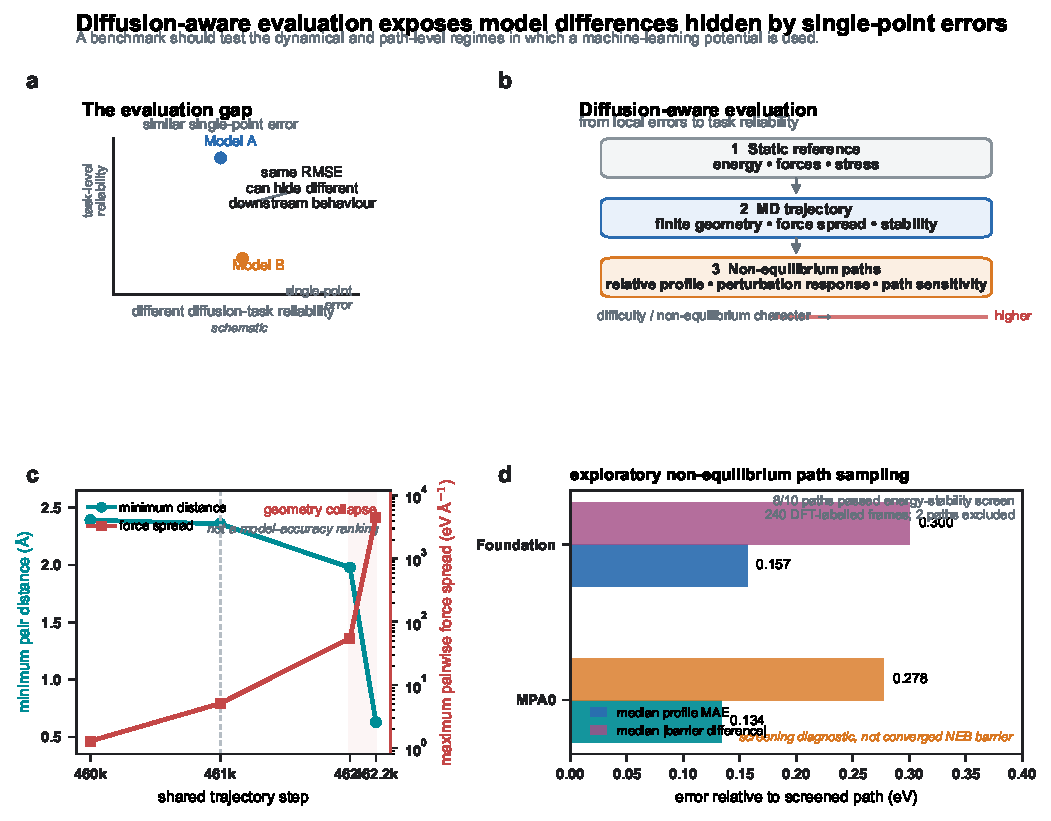
\includegraphics[width=\linewidth,height=0.42\textheight,keepaspectratio]{figure_pages/assets/fig_001.pdf}
\caption{Diffusion-aware benchmark framing, connecting the motivation, the evaluation protocol, and the audited dynamic evidence. This page shows the candidate output ``Figure1 diffusion aware evaluation'' within the audited FIG-1-DIFFUSION family. The panel identity, source scope, and current status are retained in the accompanying evidence matrix.}
\label{fig:candidate_001}
\end{figure}
\textbf{Results text draft.} This composite is intended to connect the benchmark question to the observable that is actually measured. It should be read as a context-to-result figure rather than as a claim that every downstream probe is converged.
\textbf{Discussion and boundary.} Use this figure at the Introduction/Results transition or as a high-level overview. The path-level and transport-level claims remain limited by the status fields recorded in the audit matrix.
\textbf{Article placement.} Proposed article location: Introduction/Results transition; diffusion-aware evaluation.
\textbf{Reviewer linkage:} overall status DONE.
\begin{itemize}[leftmargin=1.4em,noitemsep]
\item \textbf{REV-A4 (DONE):} Rescope generalizability claims or add an independent material/dopant validation. \emph{Completed:} The manuscript language is scoped to a candidate framework demonstrated on Cr-doped Sb2Te3; broader claims are framed as future validation. \emph{Still required:} Do not add a cross-system conclusion unless the optional second-dopant calculation is actually completed and audited.
\end{itemize}
\textbf{Evidence pointers.}
\begin{itemize}[leftmargin=1.4em,noitemsep]
\item Plot/processing script: \begingroup\scriptsize\url{main/analysis/figure1_context_method_result_20261002/figure1_nature.py}\endgroup
\item Caption/text source: \begingroup\scriptsize\url{main/analysis/figure1_context_method_result_20261002/figures/figure1_caption.md}\endgroup
\end{itemize}
\statusline{\textbf{Audit gap / next action:} Not yet mapped to the revision1 TeX figure labels}
\vfill
\clearpage
\section{FIG-002 --- Mace 1ns evidence aware benchmark}
\label{figpage:fig-002}
\textbf{Group:} MD-1NS\quad \textbf{Evidence chain:} traceable\quad \textbf{Status:} publication
\begin{figure}[H]
\centering
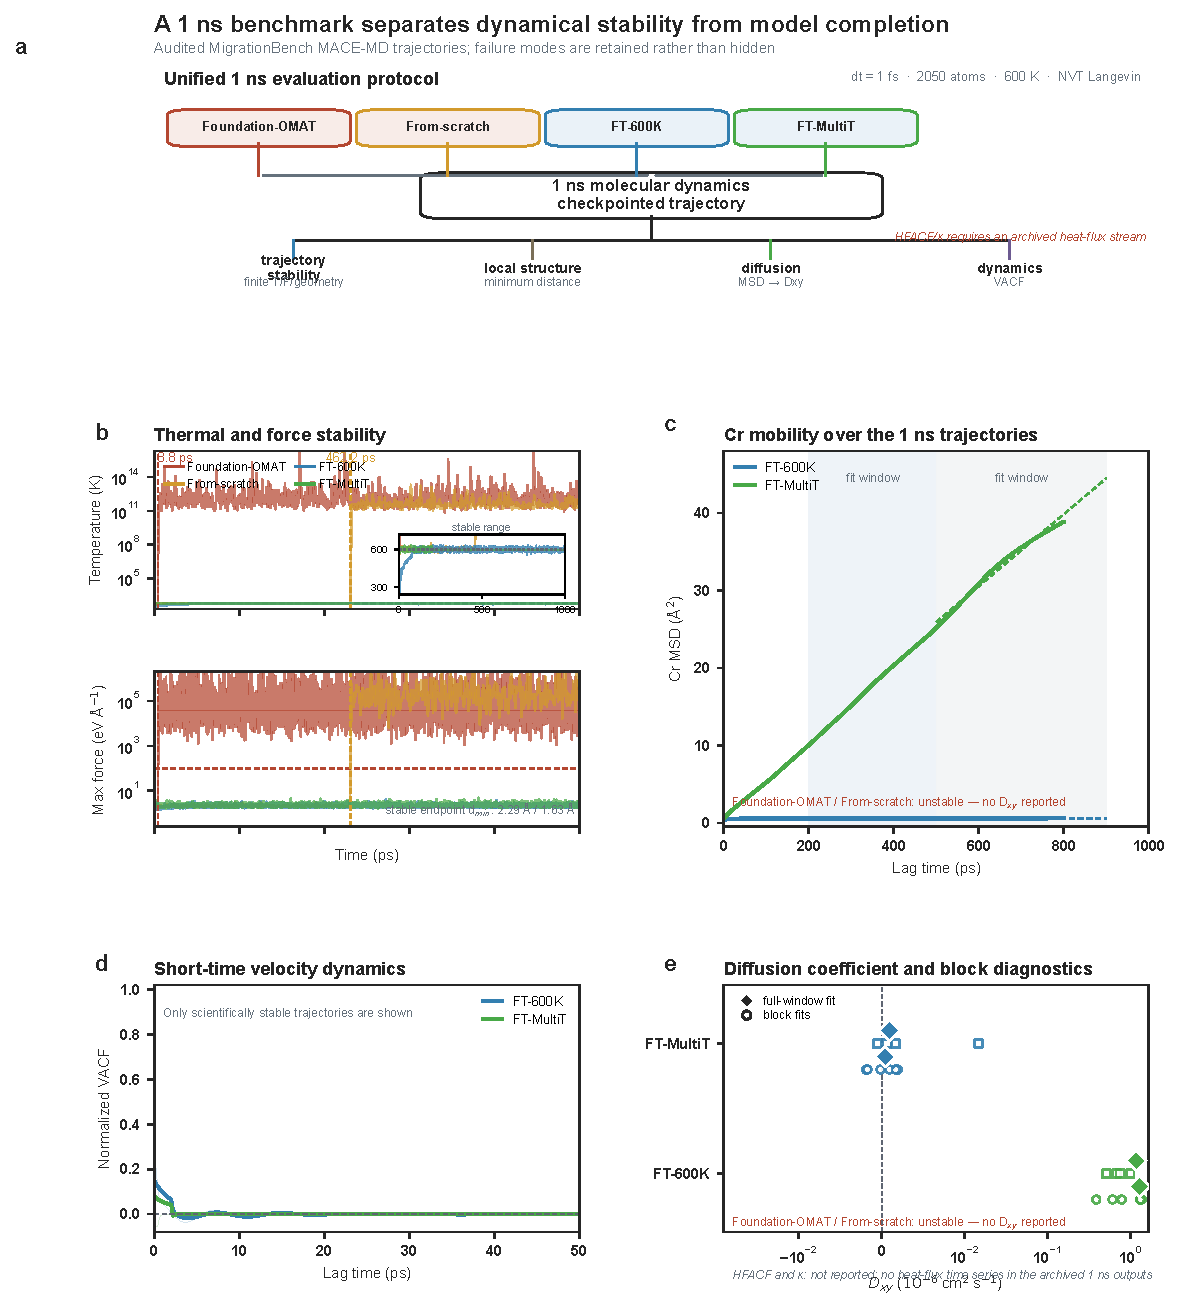
\includegraphics[width=\linewidth,height=0.42\textheight,keepaspectratio]{figure_pages/assets/fig_002.pdf}
\caption{One-nanosecond molecular-dynamics stability and diffusion diagnostics across the audited model set. This page shows the candidate output ``Mace 1ns evidence aware benchmark'' within the audited MD-1NS family. The panel identity, source scope, and current status are retained in the accompanying evidence matrix.}
\label{fig:candidate_002}
\end{figure}
\textbf{Results text draft.} The panels summarize trajectory integrity, thermal/force behavior, structural diagnostics, and diffusion observables where the required trajectory and convergence gates are available. Failed or excluded branches remain visible rather than being converted into numerical transport estimates.
\textbf{Discussion and boundary.} This figure can support dynamic-stability discussion. It must not be used to imply heat-flux-derived thermal conductivity when the same-campaign heat-flux series is absent; such quantities remain explicitly unavailable.
\textbf{Article placement.} Proposed article location: Results: dynamic stability and diffusion; SI transport candidate.
\textbf{Reviewer linkage:} overall status PENDING.
\begin{itemize}[leftmargin=1.4em,noitemsep]
\item \textbf{REV-C9 (PENDING):} Resolve the asymmetric FT-600K MD transport protocol and its effect on D and kappa. \emph{Completed:} Legacy FT-600K transport values are quarantined and excluded from ranking; the figure can document that boundary. \emph{Still required:} Run the corrected matched-protocol FT-600K long trajectory, block-average D/kappa, and close the multi-seed uncertainty before reporting a final transport comparison.
\end{itemize}
\textbf{Evidence pointers.}
\begin{itemize}[leftmargin=1.4em,noitemsep]
\item Data/processed: \begingroup\scriptsize\url{main/analysis/mace_1ns_publication_figure_20261005/figure_manifest.json}\endgroup
\item Data/processed: \begingroup\scriptsize\url{main/analysis/mace_1ns_publication_figure_20261005/final_benchmark_manifest.json}\endgroup
\item Plot/processing script: \begingroup\scriptsize\url{main/analysis/mace_1ns_publication_figure_20261005/plot_figure.py}\endgroup
\item Plot/processing script: \begingroup\scriptsize\url{main/analysis/mace_1ns_publication_figure_20261005/plot_final_benchmark.py}\endgroup
\item Caption/text source: \begingroup\scriptsize\url{main/analysis/mace_1ns_publication_figure_20261005/figure_caption.md}\endgroup
\item Caption/text source: \begingroup\scriptsize\url{main/analysis/mace_1ns_publication_figure_20261005/final_benchmark_caption.md}\endgroup
\end{itemize}
\statusline{\textbf{Audit gap / next action:} Article integration and heat-flux absence must remain explicit}
\vfill
\clearpage
\section{FIG-003 --- Mace 1ns final diffusion benchmark}
\label{figpage:fig-003}
\textbf{Group:} MD-1NS\quad \textbf{Evidence chain:} traceable\quad \textbf{Status:} publication
\begin{figure}[H]
\centering
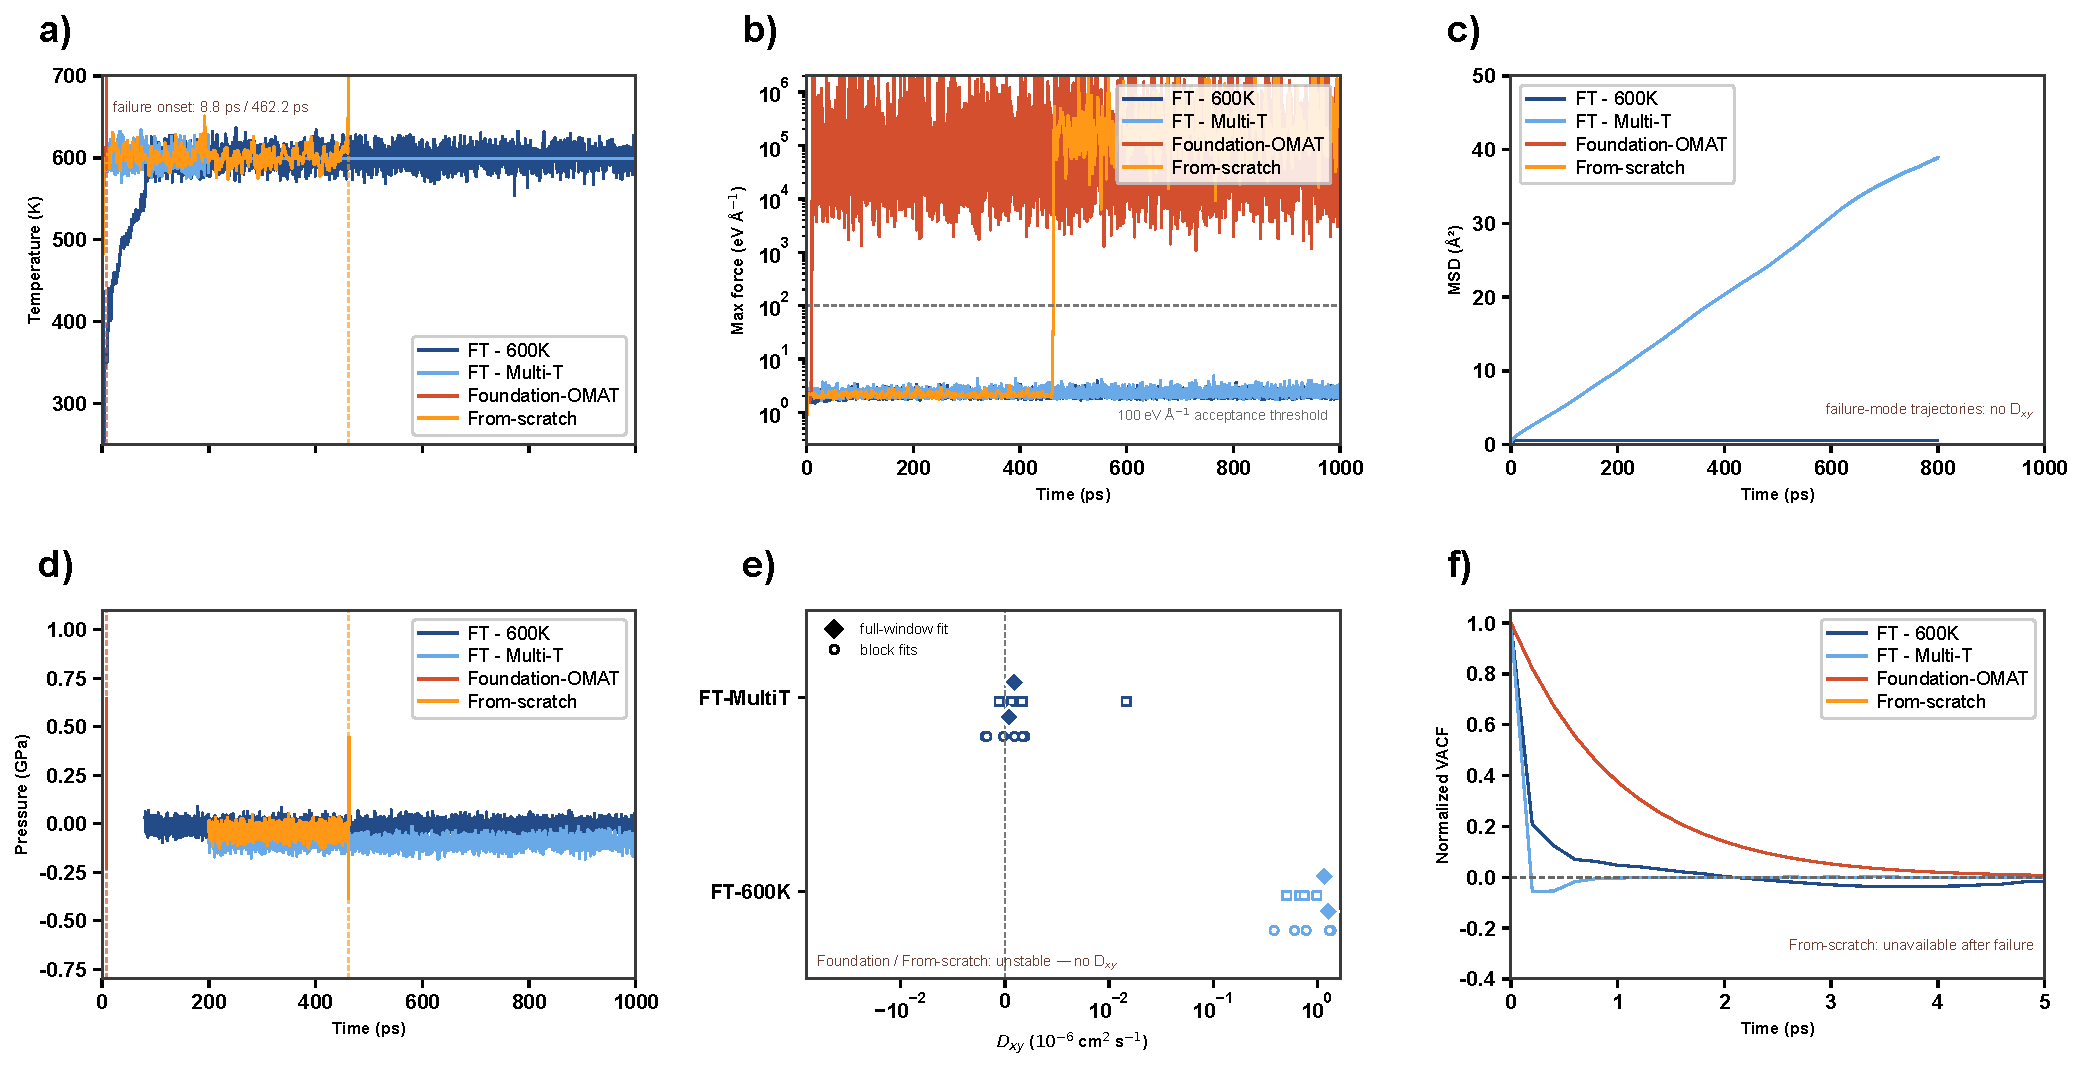
\includegraphics[width=\linewidth,height=0.42\textheight,keepaspectratio]{figure_pages/assets/fig_003.pdf}
\caption{One-nanosecond molecular-dynamics stability and diffusion diagnostics across the audited model set. This page shows the candidate output ``Mace 1ns final diffusion benchmark'' within the audited MD-1NS family. The panel identity, source scope, and current status are retained in the accompanying evidence matrix.}
\label{fig:candidate_003}
\end{figure}
\textbf{Results text draft.} The panels summarize trajectory integrity, thermal/force behavior, structural diagnostics, and diffusion observables where the required trajectory and convergence gates are available. Failed or excluded branches remain visible rather than being converted into numerical transport estimates.
\textbf{Discussion and boundary.} This figure can support dynamic-stability discussion. It must not be used to imply heat-flux-derived thermal conductivity when the same-campaign heat-flux series is absent; such quantities remain explicitly unavailable.
\textbf{Article placement.} Proposed article location: Results: dynamic stability and diffusion; SI transport candidate.
\textbf{Reviewer linkage:} overall status PENDING.
\begin{itemize}[leftmargin=1.4em,noitemsep]
\item \textbf{REV-C9 (PENDING):} Resolve the asymmetric FT-600K MD transport protocol and its effect on D and kappa. \emph{Completed:} Legacy FT-600K transport values are quarantined and excluded from ranking; the figure can document that boundary. \emph{Still required:} Run the corrected matched-protocol FT-600K long trajectory, block-average D/kappa, and close the multi-seed uncertainty before reporting a final transport comparison.
\end{itemize}
\textbf{Evidence pointers.}
\begin{itemize}[leftmargin=1.4em,noitemsep]
\item Data/processed: \begingroup\scriptsize\url{main/analysis/mace_1ns_publication_figure_20261005/figure_manifest.json}\endgroup
\item Data/processed: \begingroup\scriptsize\url{main/analysis/mace_1ns_publication_figure_20261005/final_benchmark_manifest.json}\endgroup
\item Plot/processing script: \begingroup\scriptsize\url{main/analysis/mace_1ns_publication_figure_20261005/plot_figure.py}\endgroup
\item Plot/processing script: \begingroup\scriptsize\url{main/analysis/mace_1ns_publication_figure_20261005/plot_final_benchmark.py}\endgroup
\item Caption/text source: \begingroup\scriptsize\url{main/analysis/mace_1ns_publication_figure_20261005/figure_caption.md}\endgroup
\item Caption/text source: \begingroup\scriptsize\url{main/analysis/mace_1ns_publication_figure_20261005/final_benchmark_caption.md}\endgroup
\end{itemize}
\statusline{\textbf{Audit gap / next action:} Article integration and heat-flux absence must remain explicit}
\vfill
\clearpage
\section{FIG-004 --- Mace 1ns overleaf a to g template}
\label{figpage:fig-004}
\textbf{Group:} MD-1NS\quad \textbf{Evidence chain:} traceable\quad \textbf{Status:} publication
\begin{figure}[H]
\centering
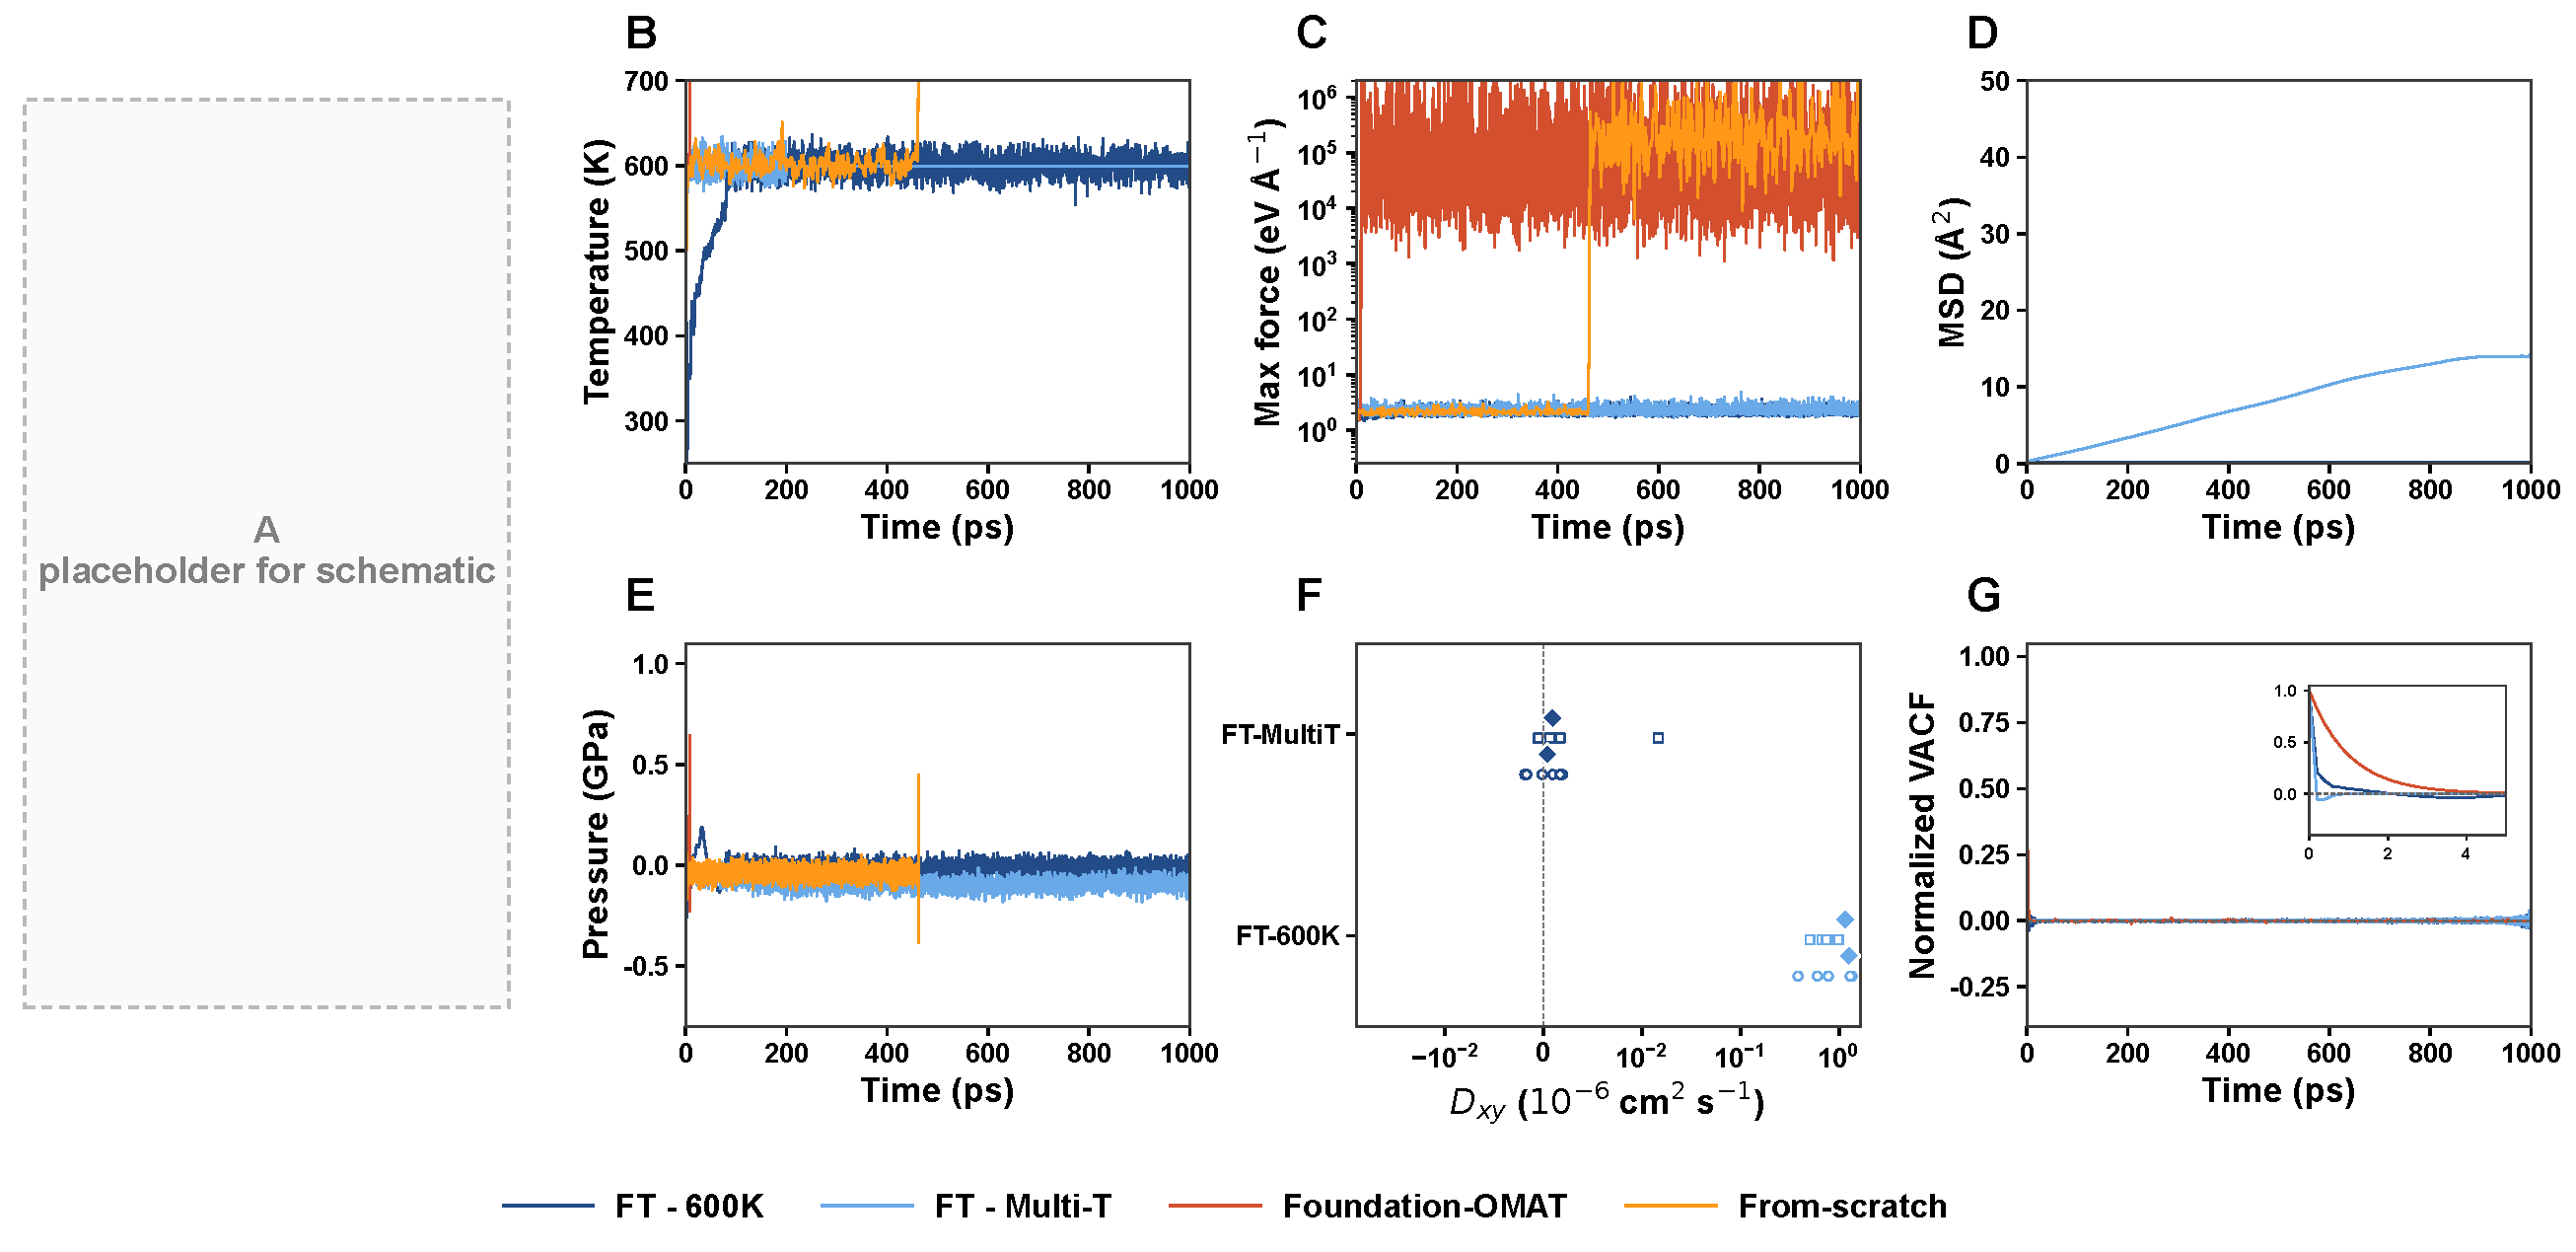
\includegraphics[width=\linewidth,height=0.42\textheight,keepaspectratio]{figure_pages/assets/fig_004.pdf}
\caption{One-nanosecond molecular-dynamics stability and diffusion diagnostics across the audited model set. This page shows the candidate output ``Mace 1ns overleaf a to g template'' within the audited MD-1NS family. The panel identity, source scope, and current status are retained in the accompanying evidence matrix.}
\label{fig:candidate_004}
\end{figure}
\textbf{Results text draft.} The panels summarize trajectory integrity, thermal/force behavior, structural diagnostics, and diffusion observables where the required trajectory and convergence gates are available. Failed or excluded branches remain visible rather than being converted into numerical transport estimates.
\textbf{Discussion and boundary.} This figure can support dynamic-stability discussion. It must not be used to imply heat-flux-derived thermal conductivity when the same-campaign heat-flux series is absent; such quantities remain explicitly unavailable.
\textbf{Article placement.} Proposed article location: Results: dynamic stability and diffusion; SI transport candidate.
\textbf{Reviewer linkage:} overall status PENDING.
\begin{itemize}[leftmargin=1.4em,noitemsep]
\item \textbf{REV-C9 (PENDING):} Resolve the asymmetric FT-600K MD transport protocol and its effect on D and kappa. \emph{Completed:} Legacy FT-600K transport values are quarantined and excluded from ranking; the figure can document that boundary. \emph{Still required:} Run the corrected matched-protocol FT-600K long trajectory, block-average D/kappa, and close the multi-seed uncertainty before reporting a final transport comparison.
\end{itemize}
\textbf{Evidence pointers.}
\begin{itemize}[leftmargin=1.4em,noitemsep]
\item Data/processed: \begingroup\scriptsize\url{main/analysis/mace_1ns_publication_figure_20261005/figure_manifest.json}\endgroup
\item Data/processed: \begingroup\scriptsize\url{main/analysis/mace_1ns_publication_figure_20261005/final_benchmark_manifest.json}\endgroup
\item Plot/processing script: \begingroup\scriptsize\url{main/analysis/mace_1ns_publication_figure_20261005/plot_figure.py}\endgroup
\item Plot/processing script: \begingroup\scriptsize\url{main/analysis/mace_1ns_publication_figure_20261005/plot_final_benchmark.py}\endgroup
\item Caption/text source: \begingroup\scriptsize\url{main/analysis/mace_1ns_publication_figure_20261005/figure_caption.md}\endgroup
\item Caption/text source: \begingroup\scriptsize\url{main/analysis/mace_1ns_publication_figure_20261005/final_benchmark_caption.md}\endgroup
\end{itemize}
\statusline{\textbf{Audit gap / next action:} Article integration and heat-flux absence must remain explicit}
\vfill
\clearpage
\section{FIG-005 --- Mace 1ns overleaf b to g}
\label{figpage:fig-005}
\textbf{Group:} MD-1NS\quad \textbf{Evidence chain:} traceable\quad \textbf{Status:} publication
\begin{figure}[H]
\centering
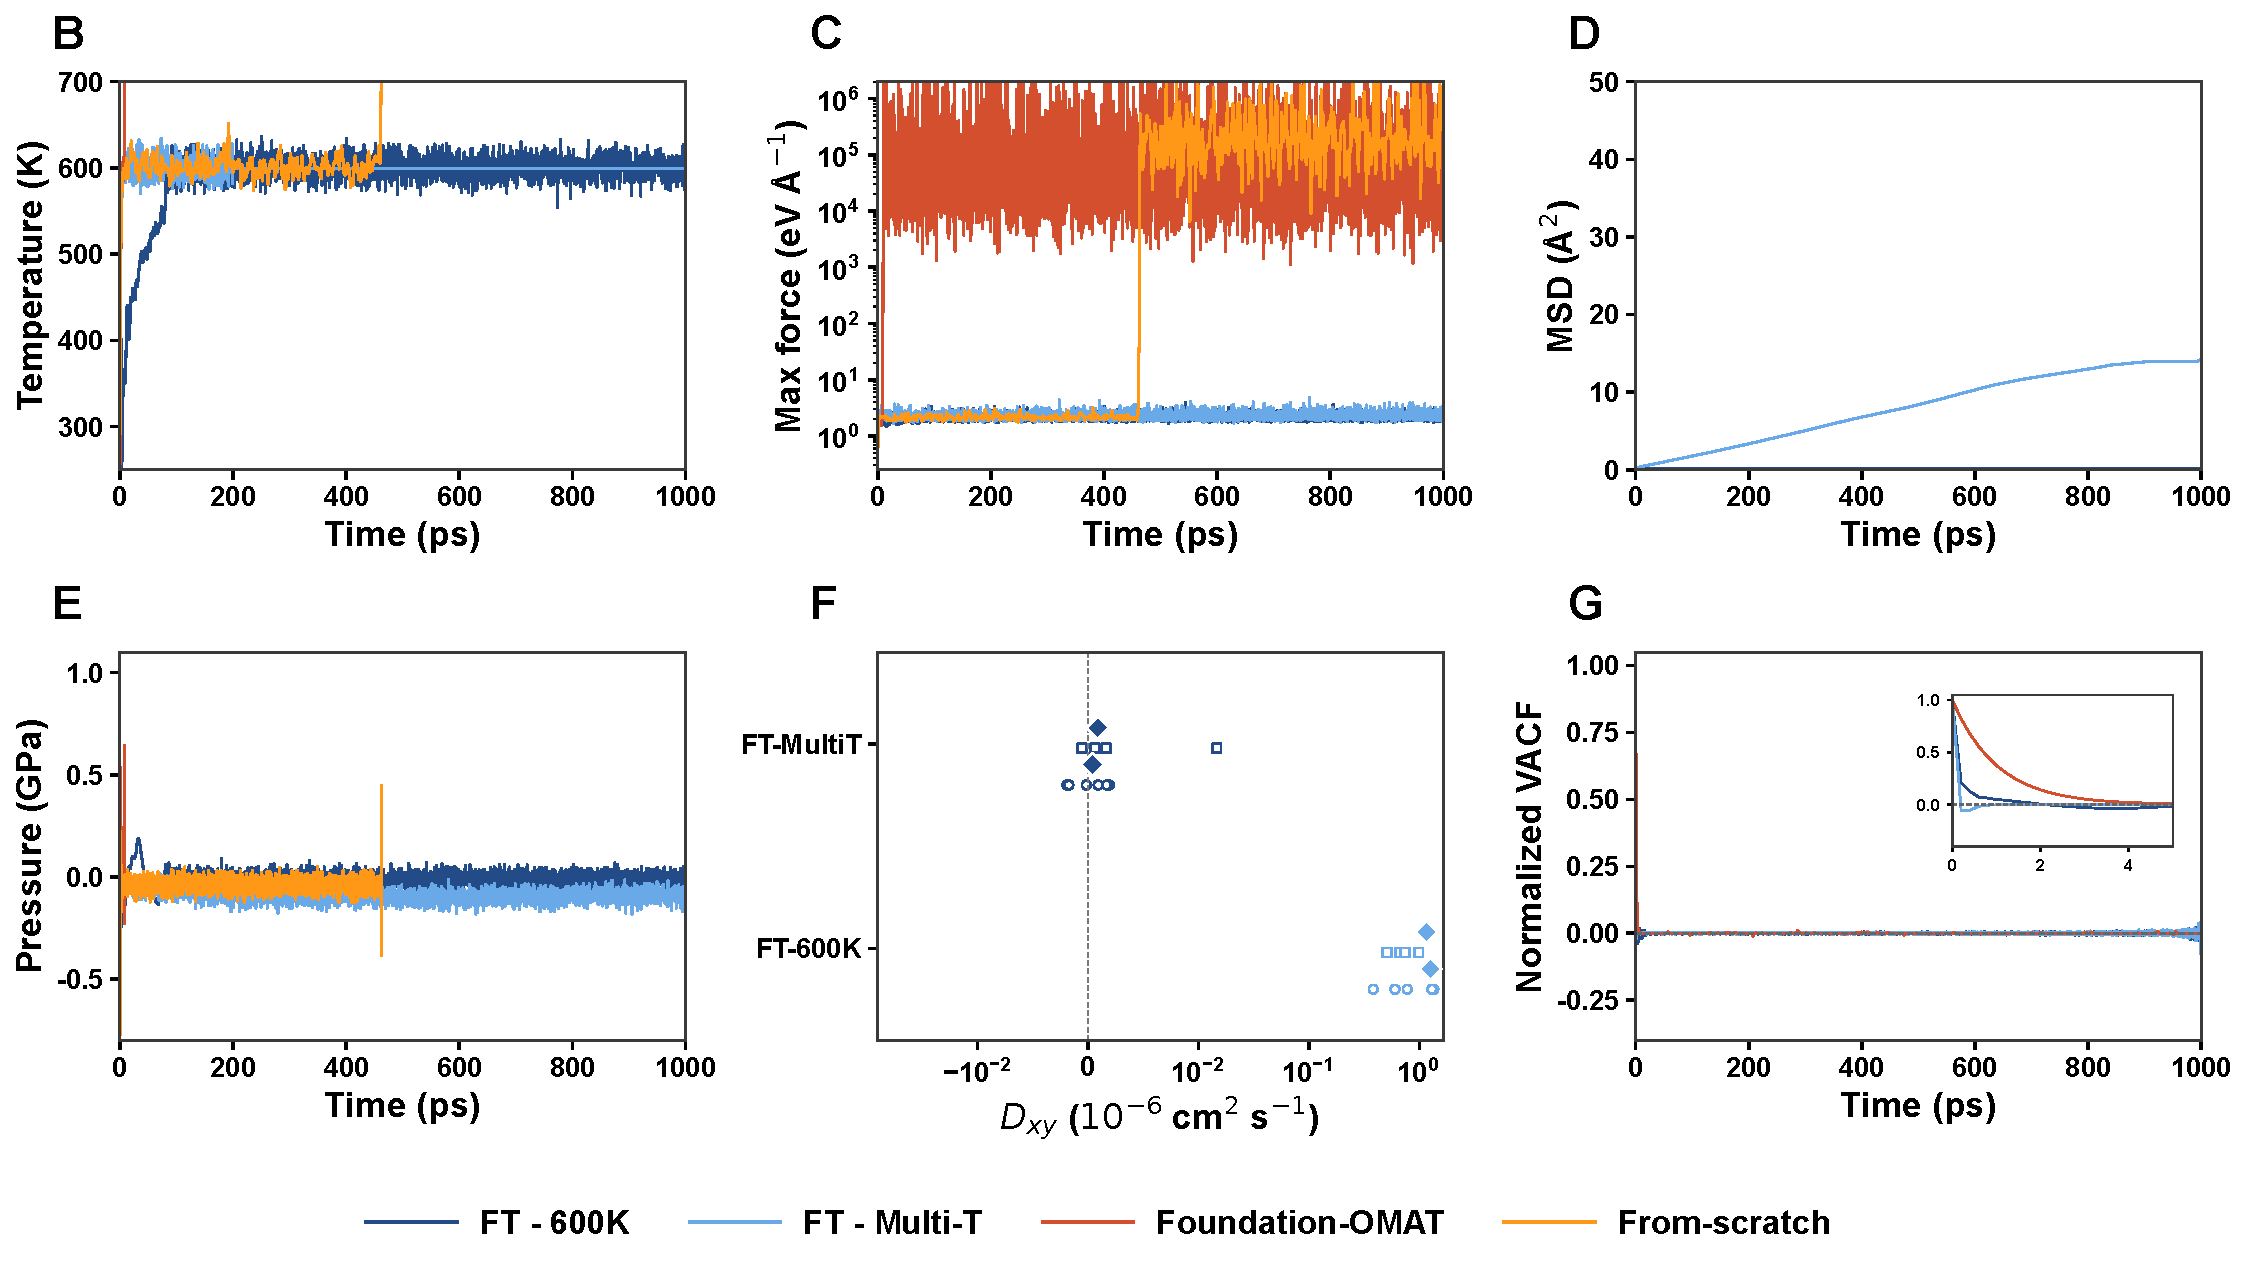
\includegraphics[width=\linewidth,height=0.42\textheight,keepaspectratio]{figure_pages/assets/fig_005.pdf}
\caption{One-nanosecond molecular-dynamics stability and diffusion diagnostics across the audited model set. This page shows the candidate output ``Mace 1ns overleaf b to g'' within the audited MD-1NS family. The panel identity, source scope, and current status are retained in the accompanying evidence matrix.}
\label{fig:candidate_005}
\end{figure}
\textbf{Results text draft.} The panels summarize trajectory integrity, thermal/force behavior, structural diagnostics, and diffusion observables where the required trajectory and convergence gates are available. Failed or excluded branches remain visible rather than being converted into numerical transport estimates.
\textbf{Discussion and boundary.} This figure can support dynamic-stability discussion. It must not be used to imply heat-flux-derived thermal conductivity when the same-campaign heat-flux series is absent; such quantities remain explicitly unavailable.
\textbf{Article placement.} Proposed article location: Results: dynamic stability and diffusion; SI transport candidate.
\textbf{Reviewer linkage:} overall status PENDING.
\begin{itemize}[leftmargin=1.4em,noitemsep]
\item \textbf{REV-C9 (PENDING):} Resolve the asymmetric FT-600K MD transport protocol and its effect on D and kappa. \emph{Completed:} Legacy FT-600K transport values are quarantined and excluded from ranking; the figure can document that boundary. \emph{Still required:} Run the corrected matched-protocol FT-600K long trajectory, block-average D/kappa, and close the multi-seed uncertainty before reporting a final transport comparison.
\end{itemize}
\textbf{Evidence pointers.}
\begin{itemize}[leftmargin=1.4em,noitemsep]
\item Data/processed: \begingroup\scriptsize\url{main/analysis/mace_1ns_publication_figure_20261005/figure_manifest.json}\endgroup
\item Data/processed: \begingroup\scriptsize\url{main/analysis/mace_1ns_publication_figure_20261005/final_benchmark_manifest.json}\endgroup
\item Plot/processing script: \begingroup\scriptsize\url{main/analysis/mace_1ns_publication_figure_20261005/plot_figure.py}\endgroup
\item Plot/processing script: \begingroup\scriptsize\url{main/analysis/mace_1ns_publication_figure_20261005/plot_final_benchmark.py}\endgroup
\item Caption/text source: \begingroup\scriptsize\url{main/analysis/mace_1ns_publication_figure_20261005/figure_caption.md}\endgroup
\item Caption/text source: \begingroup\scriptsize\url{main/analysis/mace_1ns_publication_figure_20261005/final_benchmark_caption.md}\endgroup
\end{itemize}
\statusline{\textbf{Audit gap / next action:} Article integration and heat-flux absence must remain explicit}
\vfill
\clearpage
\section{FIG-006 --- Mace 1ns strict six axis replica}
\label{figpage:fig-006}
\textbf{Group:} MD-1NS\quad \textbf{Evidence chain:} traceable\quad \textbf{Status:} strict\_replica;publication
\begin{figure}[H]
\centering
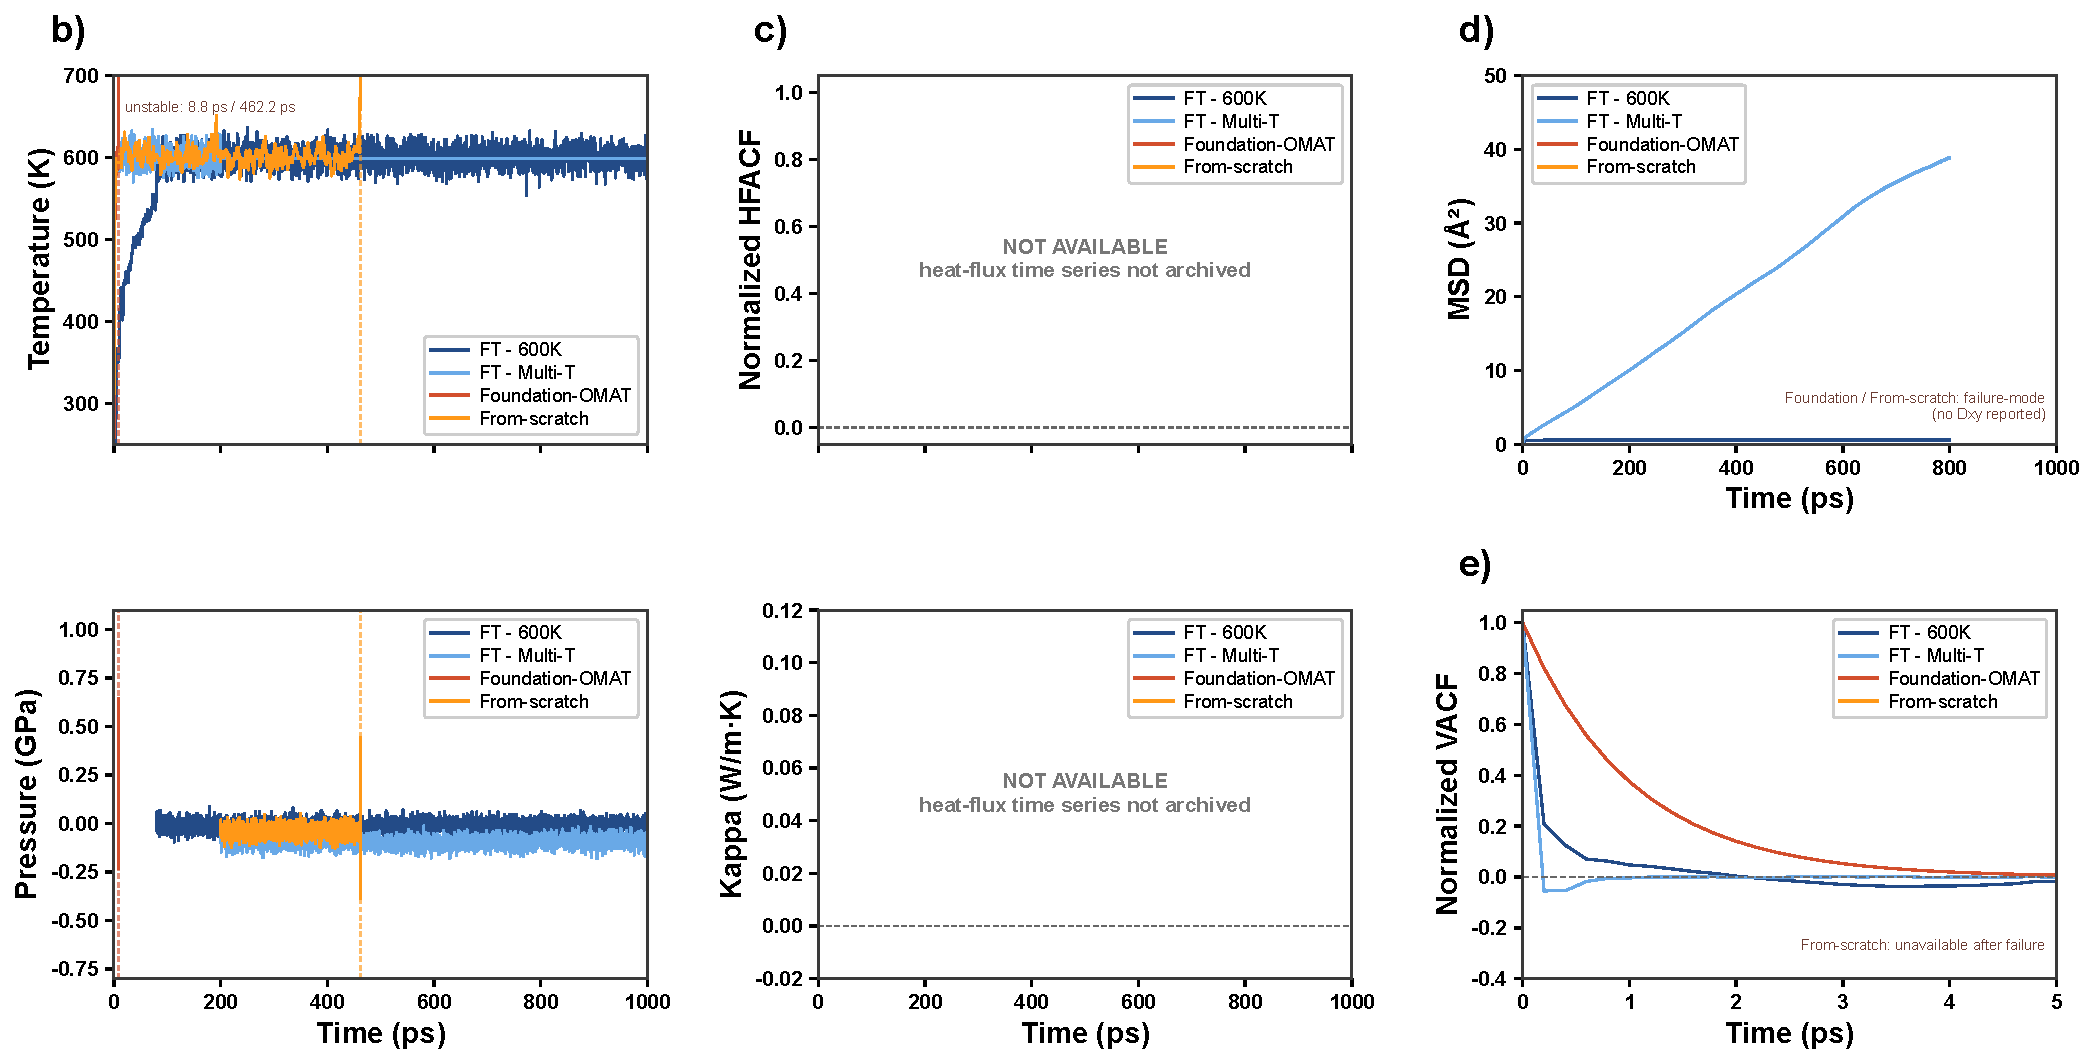
\includegraphics[width=\linewidth,height=0.42\textheight,keepaspectratio]{figure_pages/assets/fig_006.pdf}
\caption{One-nanosecond molecular-dynamics stability and diffusion diagnostics across the audited model set. This page shows the candidate output ``Mace 1ns strict six axis replica'' within the audited MD-1NS family. The panel identity, source scope, and current status are retained in the accompanying evidence matrix.}
\label{fig:candidate_006}
\end{figure}
\textbf{Results text draft.} The panels summarize trajectory integrity, thermal/force behavior, structural diagnostics, and diffusion observables where the required trajectory and convergence gates are available. Failed or excluded branches remain visible rather than being converted into numerical transport estimates.
\textbf{Discussion and boundary.} This figure can support dynamic-stability discussion. It must not be used to imply heat-flux-derived thermal conductivity when the same-campaign heat-flux series is absent; such quantities remain explicitly unavailable.
\textbf{Article placement.} Proposed article location: Results: dynamic stability and diffusion; SI transport candidate.
\textbf{Reviewer linkage:} overall status PENDING.
\begin{itemize}[leftmargin=1.4em,noitemsep]
\item \textbf{REV-C9 (PENDING):} Resolve the asymmetric FT-600K MD transport protocol and its effect on D and kappa. \emph{Completed:} Legacy FT-600K transport values are quarantined and excluded from ranking; the figure can document that boundary. \emph{Still required:} Run the corrected matched-protocol FT-600K long trajectory, block-average D/kappa, and close the multi-seed uncertainty before reporting a final transport comparison.
\end{itemize}
\textbf{Evidence pointers.}
\begin{itemize}[leftmargin=1.4em,noitemsep]
\item Data/processed: \begingroup\scriptsize\url{main/analysis/mace_1ns_publication_figure_20261005/figure_manifest.json}\endgroup
\item Data/processed: \begingroup\scriptsize\url{main/analysis/mace_1ns_publication_figure_20261005/final_benchmark_manifest.json}\endgroup
\item Plot/processing script: \begingroup\scriptsize\url{main/analysis/mace_1ns_publication_figure_20261005/plot_figure.py}\endgroup
\item Plot/processing script: \begingroup\scriptsize\url{main/analysis/mace_1ns_publication_figure_20261005/plot_final_benchmark.py}\endgroup
\item Caption/text source: \begingroup\scriptsize\url{main/analysis/mace_1ns_publication_figure_20261005/figure_caption.md}\endgroup
\item Caption/text source: \begingroup\scriptsize\url{main/analysis/mace_1ns_publication_figure_20261005/final_benchmark_caption.md}\endgroup
\end{itemize}
\statusline{\textbf{Audit gap / next action:} Article integration and heat-flux absence must remain explicit}
\vfill
\clearpage
\section{FIG-007 --- Old fig from scratch failure}
\label{figpage:fig-007}
\textbf{Group:} MD-1NS\quad \textbf{Evidence chain:} traceable\quad \textbf{Status:} publication;old\_or\_legacy
\begin{figure}[H]
\centering
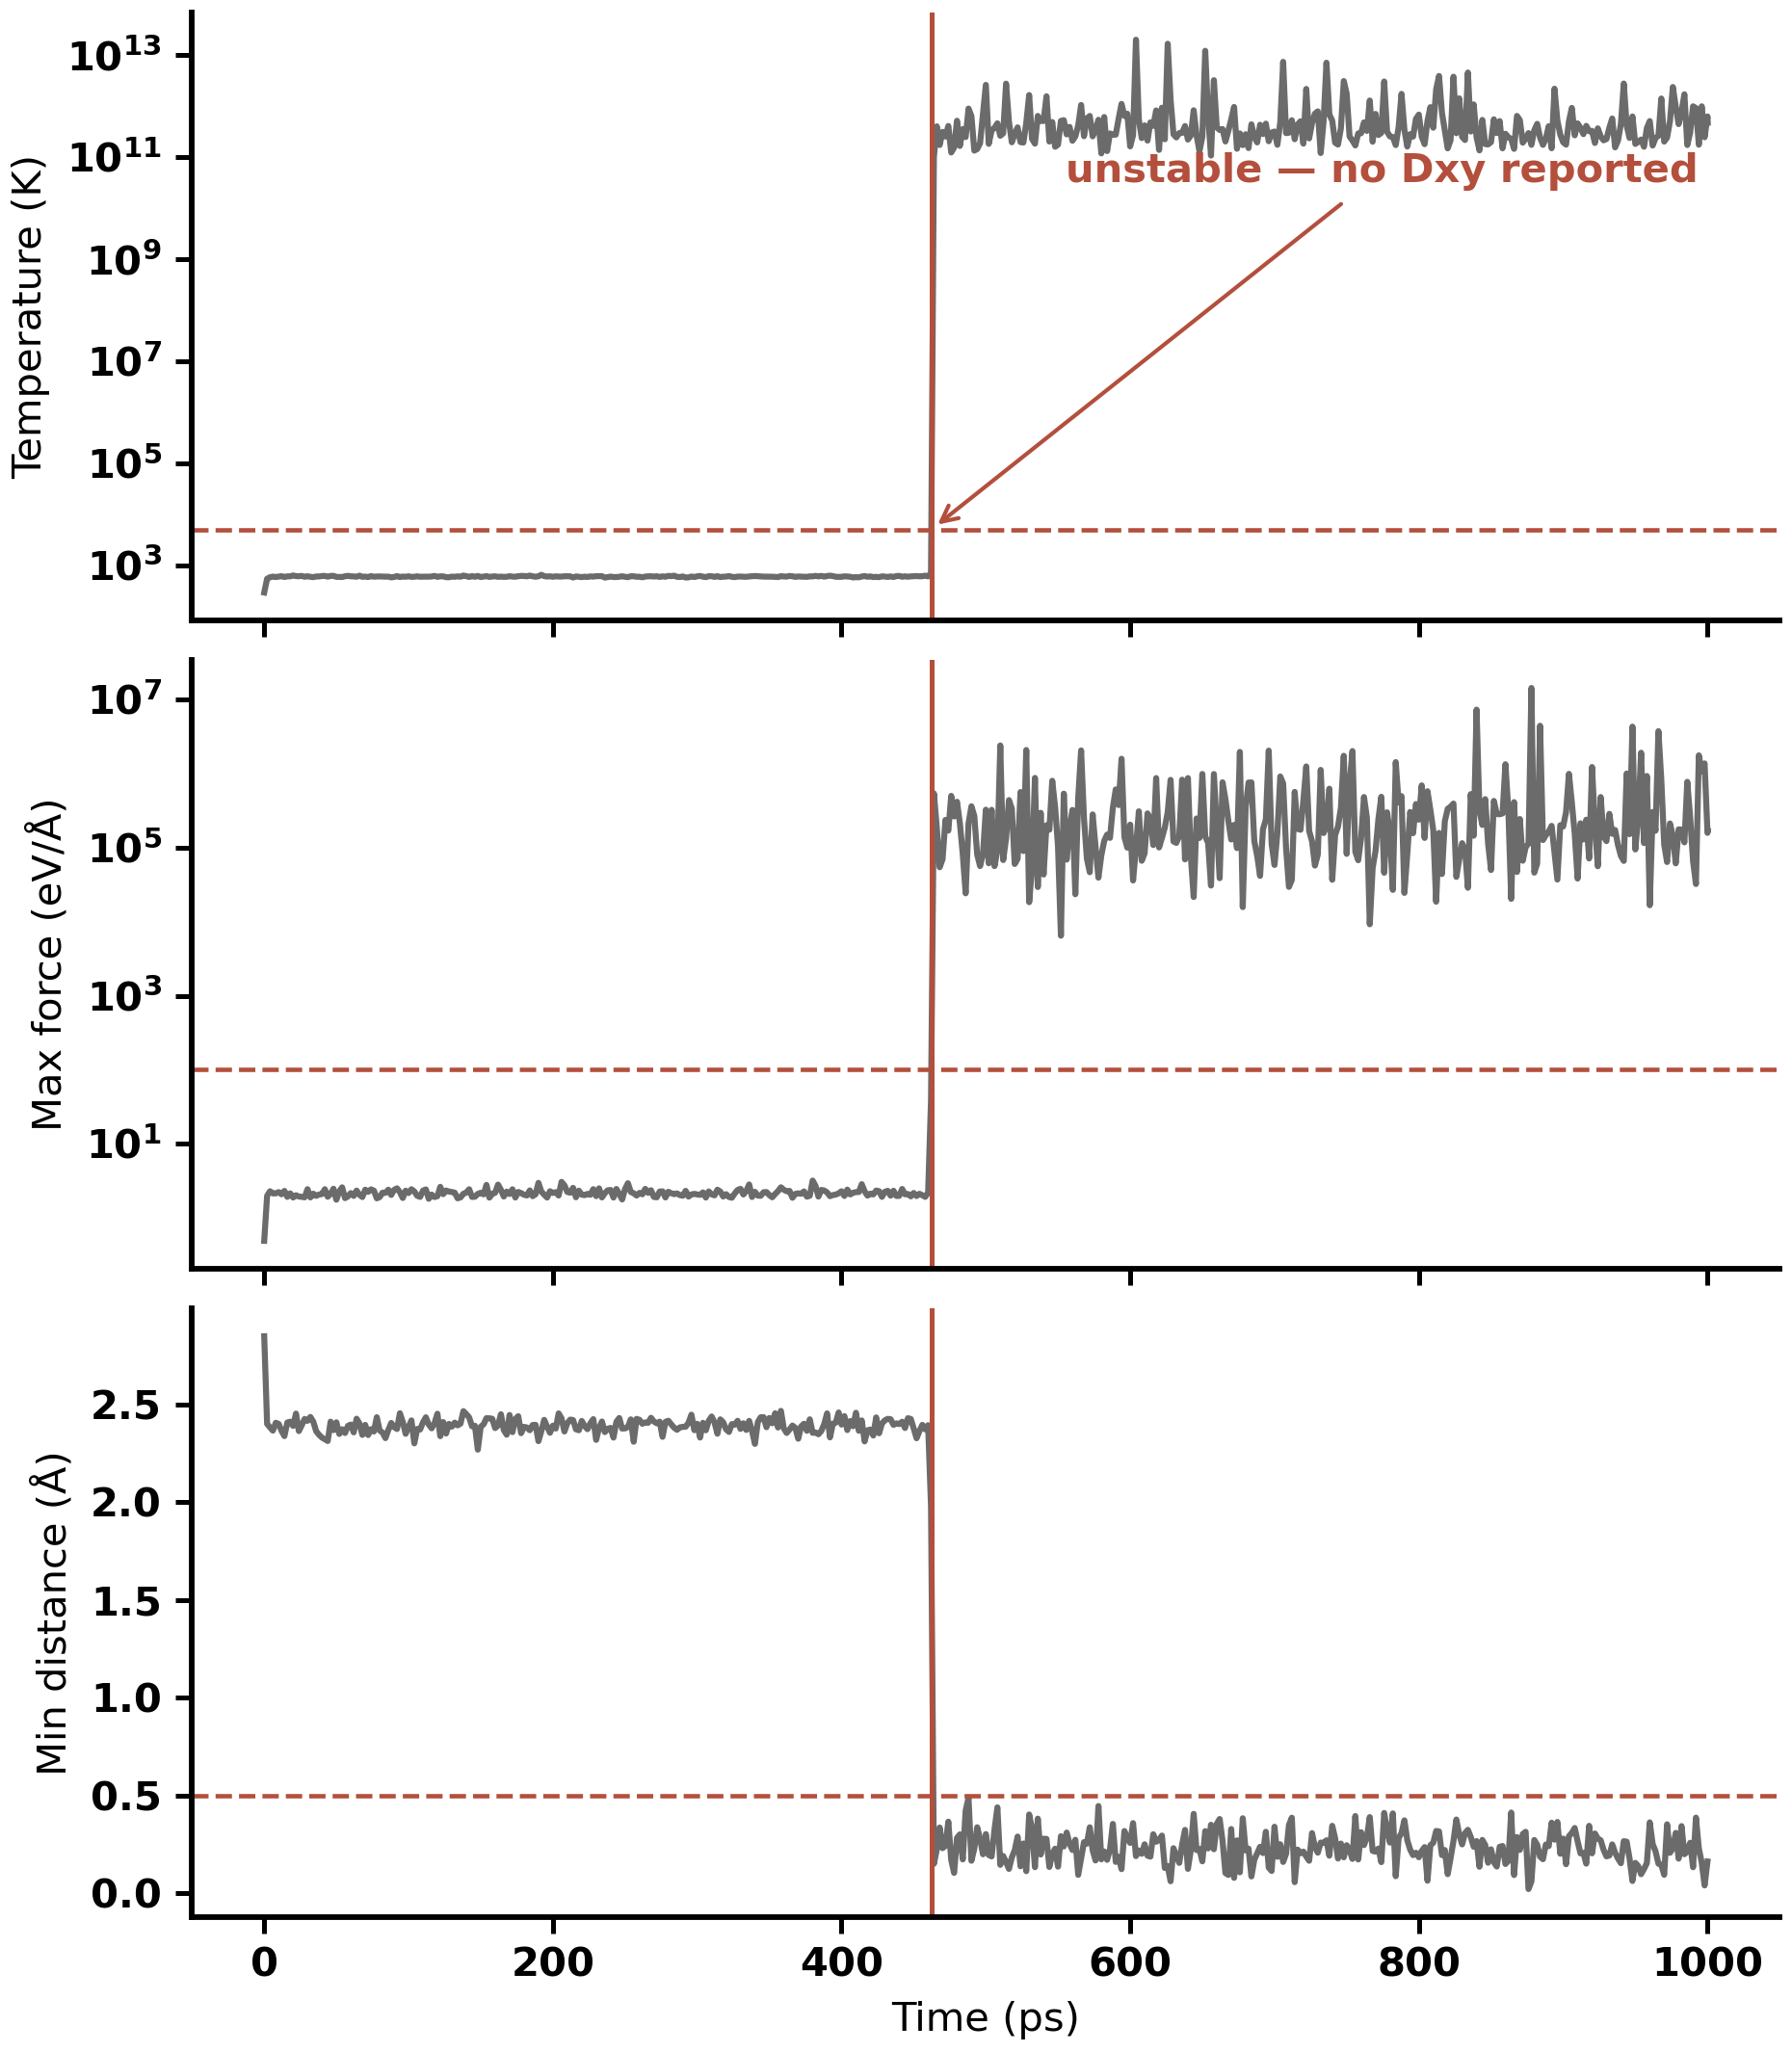
\includegraphics[width=\linewidth,height=0.42\textheight,keepaspectratio]{figure_pages/assets/fig_007.png}
\caption{One-nanosecond molecular-dynamics stability and diffusion diagnostics across the audited model set. This page shows the candidate output ``Old fig from scratch failure'' within the audited MD-1NS family. The panel identity, source scope, and current status are retained in the accompanying evidence matrix.}
\label{fig:candidate_007}
\end{figure}
\textbf{Results text draft.} The panels summarize trajectory integrity, thermal/force behavior, structural diagnostics, and diffusion observables where the required trajectory and convergence gates are available. Failed or excluded branches remain visible rather than being converted into numerical transport estimates.
\textbf{Discussion and boundary.} This figure can support dynamic-stability discussion. It must not be used to imply heat-flux-derived thermal conductivity when the same-campaign heat-flux series is absent; such quantities remain explicitly unavailable.
\textbf{Article placement.} Proposed article location: Results: dynamic stability and diffusion; SI transport candidate.
\textbf{Reviewer linkage:} overall status PENDING.
\begin{itemize}[leftmargin=1.4em,noitemsep]
\item \textbf{REV-C9 (PENDING):} Resolve the asymmetric FT-600K MD transport protocol and its effect on D and kappa. \emph{Completed:} Legacy FT-600K transport values are quarantined and excluded from ranking; the figure can document that boundary. \emph{Still required:} Run the corrected matched-protocol FT-600K long trajectory, block-average D/kappa, and close the multi-seed uncertainty before reporting a final transport comparison.
\end{itemize}
\textbf{Evidence pointers.}
\begin{itemize}[leftmargin=1.4em,noitemsep]
\item Data/processed: \begingroup\scriptsize\url{main/analysis/mace_1ns_publication_figure_20261005/figure_manifest.json}\endgroup
\item Data/processed: \begingroup\scriptsize\url{main/analysis/mace_1ns_publication_figure_20261005/final_benchmark_manifest.json}\endgroup
\item Plot/processing script: \begingroup\scriptsize\url{main/analysis/mace_1ns_publication_figure_20261005/plot_figure.py}\endgroup
\item Plot/processing script: \begingroup\scriptsize\url{main/analysis/mace_1ns_publication_figure_20261005/plot_final_benchmark.py}\endgroup
\item Caption/text source: \begingroup\scriptsize\url{main/analysis/mace_1ns_publication_figure_20261005/figure_caption.md}\endgroup
\item Caption/text source: \begingroup\scriptsize\url{main/analysis/mace_1ns_publication_figure_20261005/final_benchmark_caption.md}\endgroup
\end{itemize}
\statusline{\textbf{Audit gap / next action:} Article integration and heat-flux absence must remain explicit}
\vfill
\clearpage
\section{FIG-008 --- Old fig msd}
\label{figpage:fig-008}
\textbf{Group:} MD-1NS\quad \textbf{Evidence chain:} traceable\quad \textbf{Status:} publication;old\_or\_legacy
\begin{figure}[H]
\centering
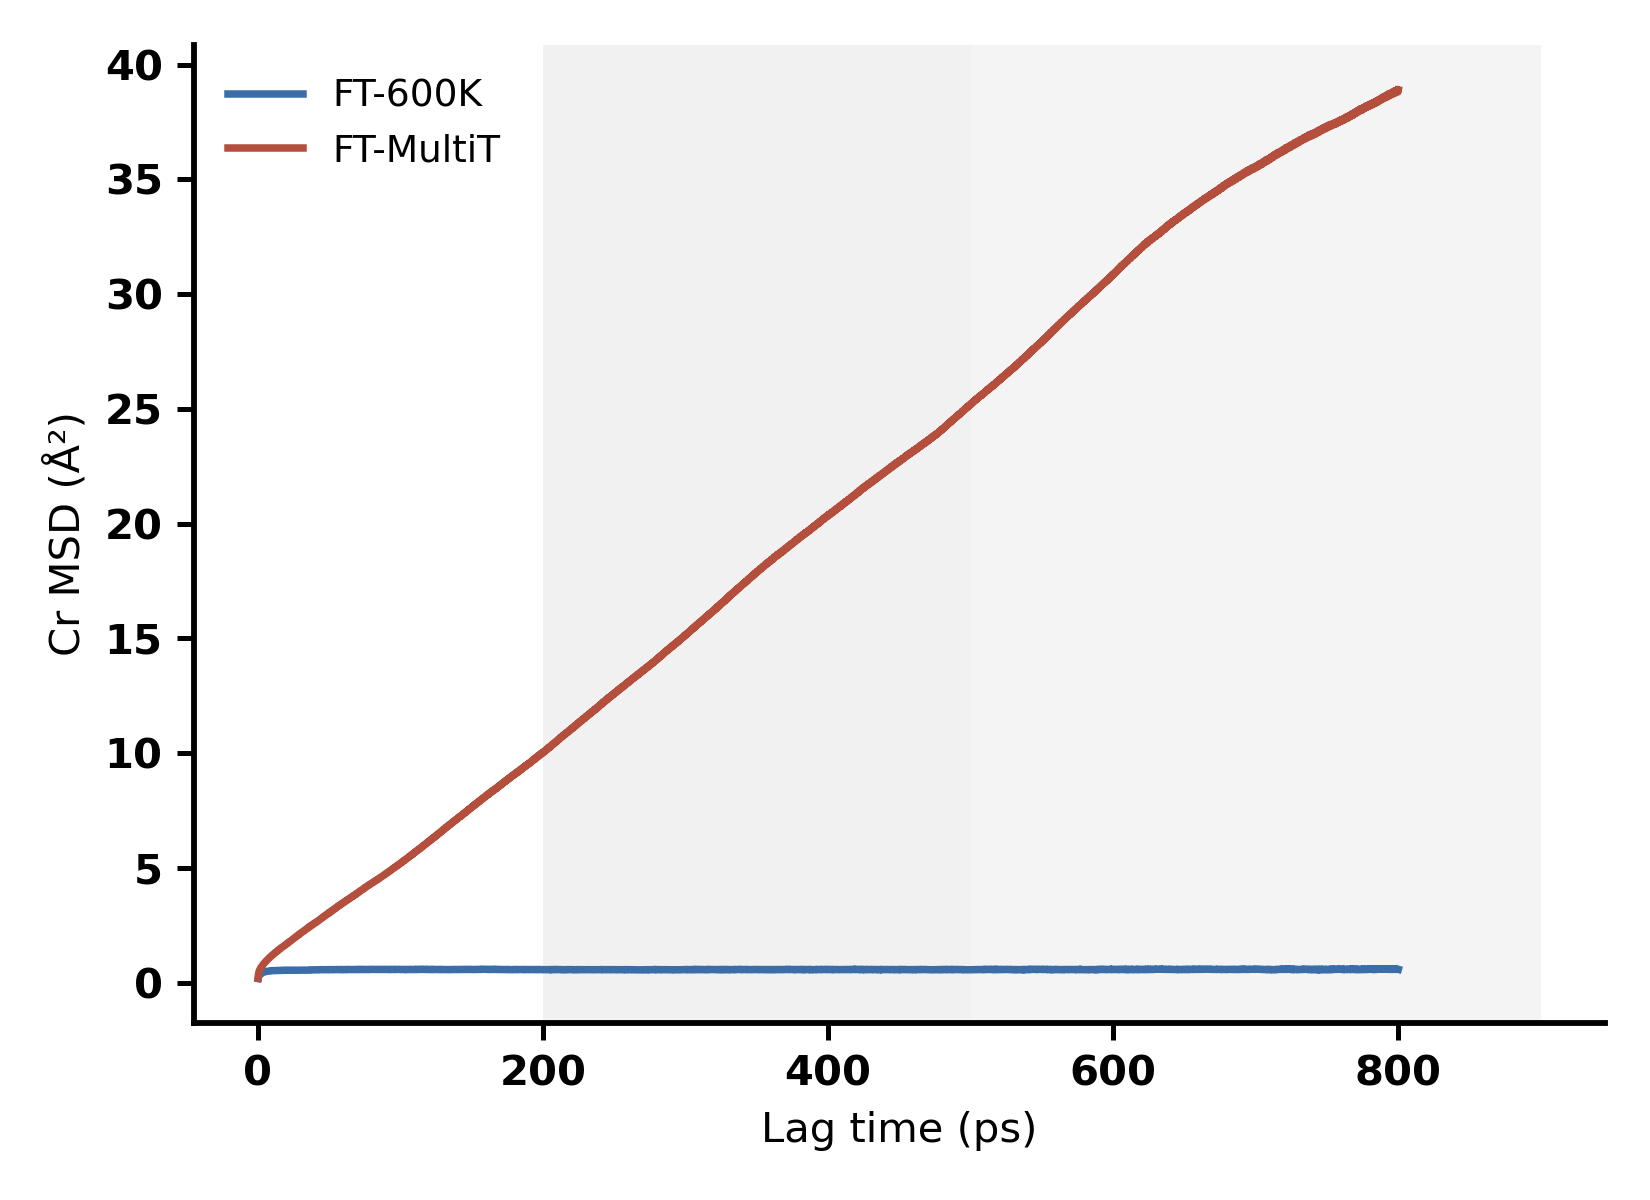
\includegraphics[width=\linewidth,height=0.42\textheight,keepaspectratio]{figure_pages/assets/fig_008.png}
\caption{One-nanosecond molecular-dynamics stability and diffusion diagnostics across the audited model set. This page shows the candidate output ``Old fig msd'' within the audited MD-1NS family. The panel identity, source scope, and current status are retained in the accompanying evidence matrix.}
\label{fig:candidate_008}
\end{figure}
\textbf{Results text draft.} The panels summarize trajectory integrity, thermal/force behavior, structural diagnostics, and diffusion observables where the required trajectory and convergence gates are available. Failed or excluded branches remain visible rather than being converted into numerical transport estimates.
\textbf{Discussion and boundary.} This figure can support dynamic-stability discussion. It must not be used to imply heat-flux-derived thermal conductivity when the same-campaign heat-flux series is absent; such quantities remain explicitly unavailable.
\textbf{Article placement.} Proposed article location: Results: dynamic stability and diffusion; SI transport candidate.
\textbf{Reviewer linkage:} overall status PENDING.
\begin{itemize}[leftmargin=1.4em,noitemsep]
\item \textbf{REV-C9 (PENDING):} Resolve the asymmetric FT-600K MD transport protocol and its effect on D and kappa. \emph{Completed:} Legacy FT-600K transport values are quarantined and excluded from ranking; the figure can document that boundary. \emph{Still required:} Run the corrected matched-protocol FT-600K long trajectory, block-average D/kappa, and close the multi-seed uncertainty before reporting a final transport comparison.
\end{itemize}
\textbf{Evidence pointers.}
\begin{itemize}[leftmargin=1.4em,noitemsep]
\item Data/processed: \begingroup\scriptsize\url{main/analysis/mace_1ns_publication_figure_20261005/figure_manifest.json}\endgroup
\item Data/processed: \begingroup\scriptsize\url{main/analysis/mace_1ns_publication_figure_20261005/final_benchmark_manifest.json}\endgroup
\item Plot/processing script: \begingroup\scriptsize\url{main/analysis/mace_1ns_publication_figure_20261005/plot_figure.py}\endgroup
\item Plot/processing script: \begingroup\scriptsize\url{main/analysis/mace_1ns_publication_figure_20261005/plot_final_benchmark.py}\endgroup
\item Caption/text source: \begingroup\scriptsize\url{main/analysis/mace_1ns_publication_figure_20261005/figure_caption.md}\endgroup
\item Caption/text source: \begingroup\scriptsize\url{main/analysis/mace_1ns_publication_figure_20261005/final_benchmark_caption.md}\endgroup
\end{itemize}
\statusline{\textbf{Audit gap / next action:} Article integration and heat-flux absence must remain explicit}
\vfill
\clearpage
\section{FIG-009 --- Old fig stability}
\label{figpage:fig-009}
\textbf{Group:} MD-1NS\quad \textbf{Evidence chain:} traceable\quad \textbf{Status:} publication;old\_or\_legacy
\begin{figure}[H]
\centering
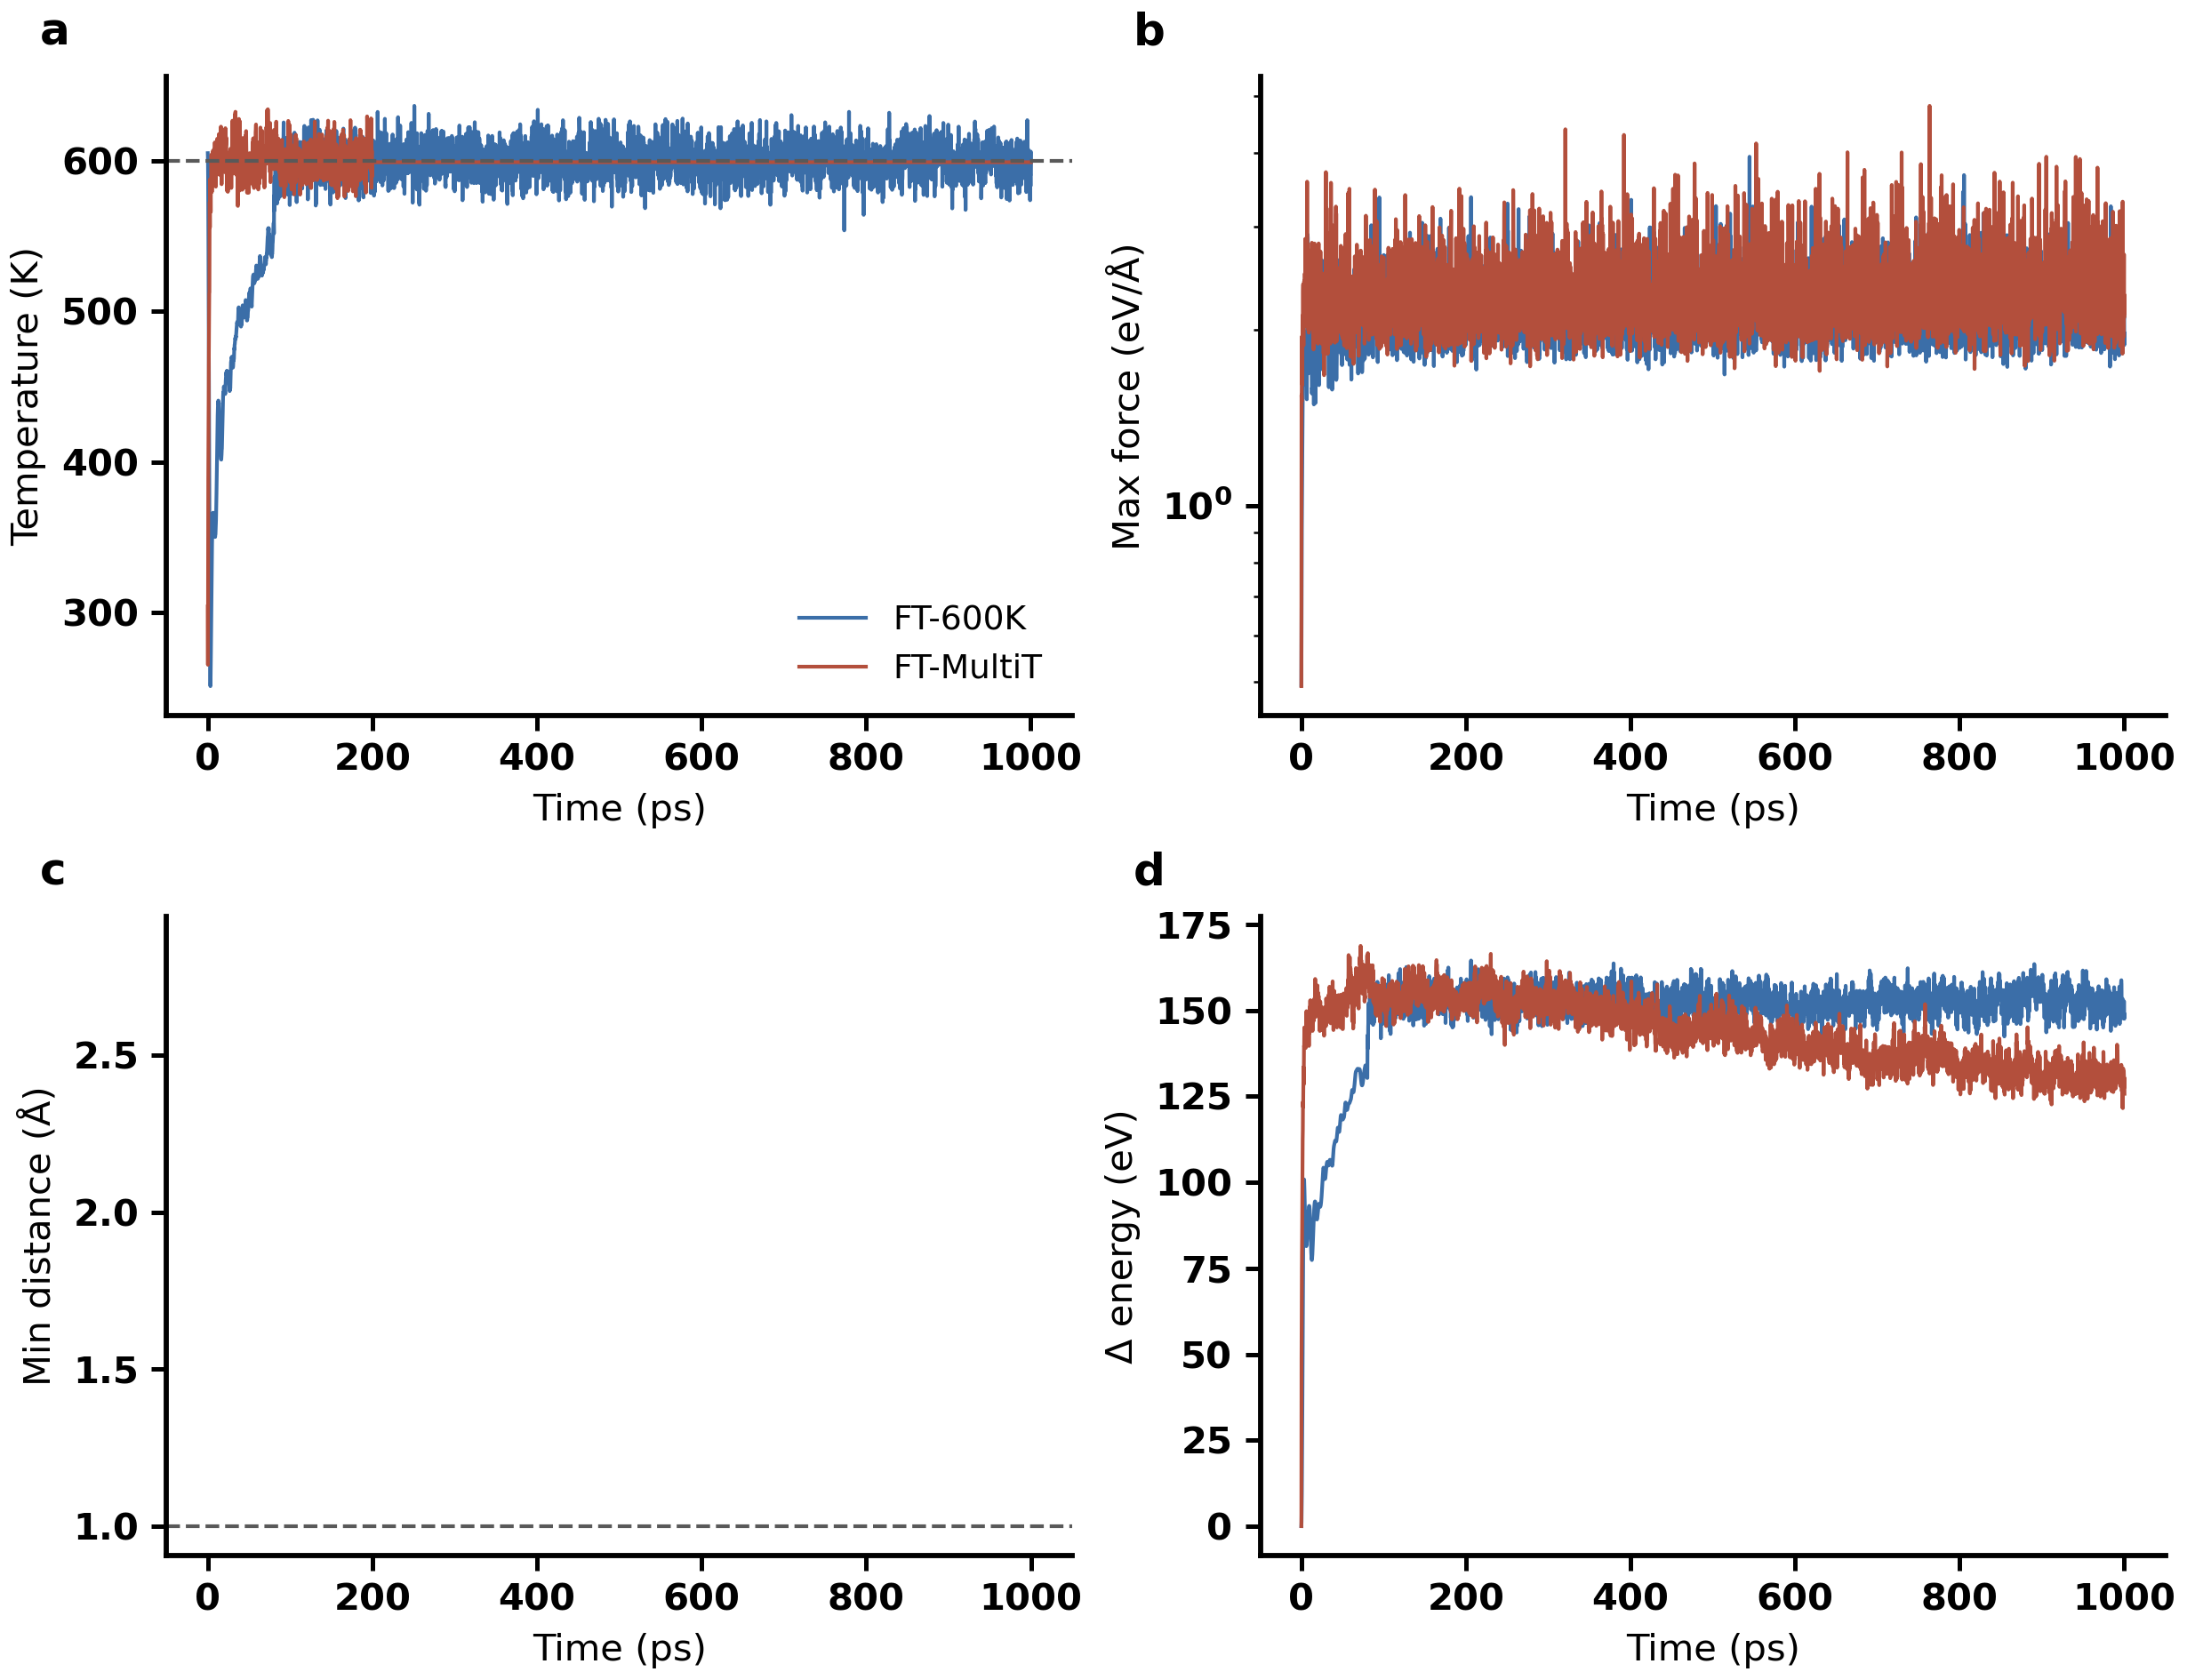
\includegraphics[width=\linewidth,height=0.42\textheight,keepaspectratio]{figure_pages/assets/fig_009.png}
\caption{One-nanosecond molecular-dynamics stability and diffusion diagnostics across the audited model set. This page shows the candidate output ``Old fig stability'' within the audited MD-1NS family. The panel identity, source scope, and current status are retained in the accompanying evidence matrix.}
\label{fig:candidate_009}
\end{figure}
\textbf{Results text draft.} The panels summarize trajectory integrity, thermal/force behavior, structural diagnostics, and diffusion observables where the required trajectory and convergence gates are available. Failed or excluded branches remain visible rather than being converted into numerical transport estimates.
\textbf{Discussion and boundary.} This figure can support dynamic-stability discussion. It must not be used to imply heat-flux-derived thermal conductivity when the same-campaign heat-flux series is absent; such quantities remain explicitly unavailable.
\textbf{Article placement.} Proposed article location: Results: dynamic stability and diffusion; SI transport candidate.
\textbf{Reviewer linkage:} overall status PENDING.
\begin{itemize}[leftmargin=1.4em,noitemsep]
\item \textbf{REV-C9 (PENDING):} Resolve the asymmetric FT-600K MD transport protocol and its effect on D and kappa. \emph{Completed:} Legacy FT-600K transport values are quarantined and excluded from ranking; the figure can document that boundary. \emph{Still required:} Run the corrected matched-protocol FT-600K long trajectory, block-average D/kappa, and close the multi-seed uncertainty before reporting a final transport comparison.
\end{itemize}
\textbf{Evidence pointers.}
\begin{itemize}[leftmargin=1.4em,noitemsep]
\item Data/processed: \begingroup\scriptsize\url{main/analysis/mace_1ns_publication_figure_20261005/figure_manifest.json}\endgroup
\item Data/processed: \begingroup\scriptsize\url{main/analysis/mace_1ns_publication_figure_20261005/final_benchmark_manifest.json}\endgroup
\item Plot/processing script: \begingroup\scriptsize\url{main/analysis/mace_1ns_publication_figure_20261005/plot_figure.py}\endgroup
\item Plot/processing script: \begingroup\scriptsize\url{main/analysis/mace_1ns_publication_figure_20261005/plot_final_benchmark.py}\endgroup
\item Caption/text source: \begingroup\scriptsize\url{main/analysis/mace_1ns_publication_figure_20261005/figure_caption.md}\endgroup
\item Caption/text source: \begingroup\scriptsize\url{main/analysis/mace_1ns_publication_figure_20261005/final_benchmark_caption.md}\endgroup
\end{itemize}
\statusline{\textbf{Audit gap / next action:} Article integration and heat-flux absence must remain explicit}
\vfill
\clearpage
\section{FIG-010 --- Old fig vacf}
\label{figpage:fig-010}
\textbf{Group:} MD-1NS\quad \textbf{Evidence chain:} traceable\quad \textbf{Status:} publication;old\_or\_legacy
\begin{figure}[H]
\centering
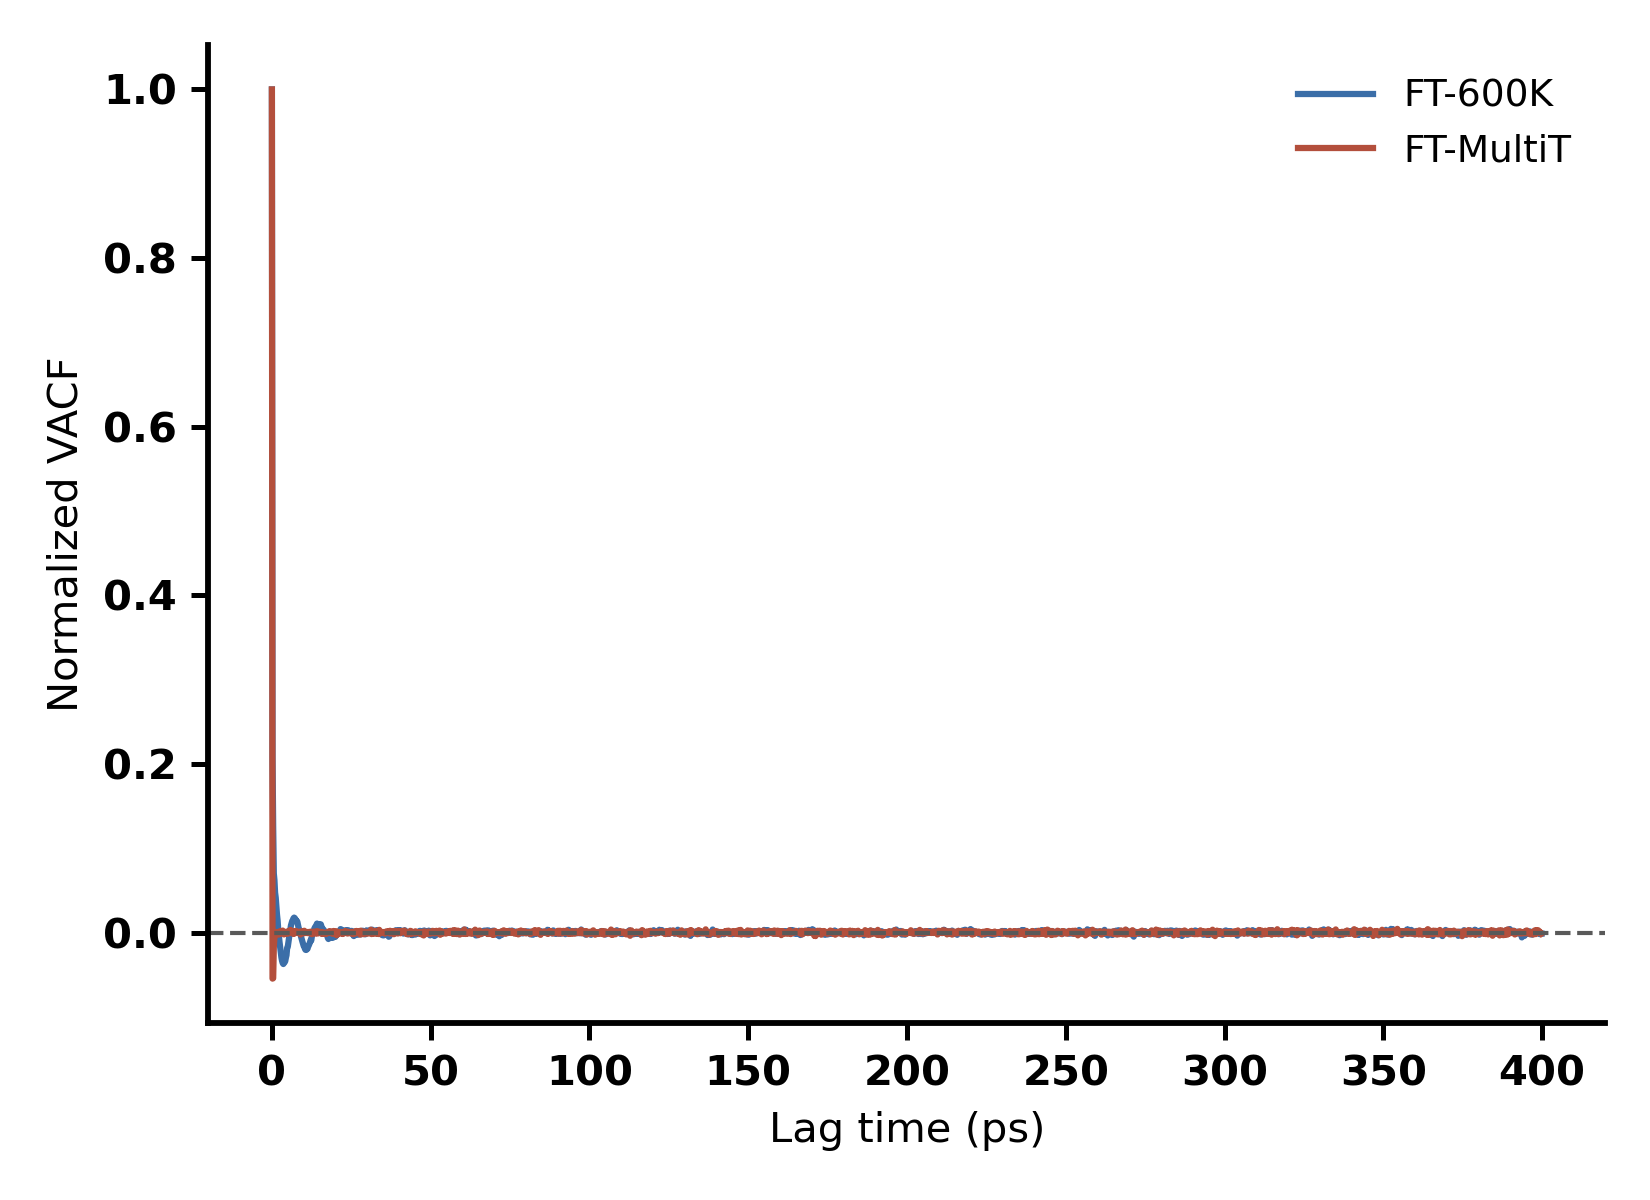
\includegraphics[width=\linewidth,height=0.42\textheight,keepaspectratio]{figure_pages/assets/fig_010.png}
\caption{One-nanosecond molecular-dynamics stability and diffusion diagnostics across the audited model set. This page shows the candidate output ``Old fig vacf'' within the audited MD-1NS family. The panel identity, source scope, and current status are retained in the accompanying evidence matrix.}
\label{fig:candidate_010}
\end{figure}
\textbf{Results text draft.} The panels summarize trajectory integrity, thermal/force behavior, structural diagnostics, and diffusion observables where the required trajectory and convergence gates are available. Failed or excluded branches remain visible rather than being converted into numerical transport estimates.
\textbf{Discussion and boundary.} This figure can support dynamic-stability discussion. It must not be used to imply heat-flux-derived thermal conductivity when the same-campaign heat-flux series is absent; such quantities remain explicitly unavailable.
\textbf{Article placement.} Proposed article location: Results: dynamic stability and diffusion; SI transport candidate.
\textbf{Reviewer linkage:} overall status PENDING.
\begin{itemize}[leftmargin=1.4em,noitemsep]
\item \textbf{REV-C9 (PENDING):} Resolve the asymmetric FT-600K MD transport protocol and its effect on D and kappa. \emph{Completed:} Legacy FT-600K transport values are quarantined and excluded from ranking; the figure can document that boundary. \emph{Still required:} Run the corrected matched-protocol FT-600K long trajectory, block-average D/kappa, and close the multi-seed uncertainty before reporting a final transport comparison.
\end{itemize}
\textbf{Evidence pointers.}
\begin{itemize}[leftmargin=1.4em,noitemsep]
\item Data/processed: \begingroup\scriptsize\url{main/analysis/mace_1ns_publication_figure_20261005/figure_manifest.json}\endgroup
\item Data/processed: \begingroup\scriptsize\url{main/analysis/mace_1ns_publication_figure_20261005/final_benchmark_manifest.json}\endgroup
\item Plot/processing script: \begingroup\scriptsize\url{main/analysis/mace_1ns_publication_figure_20261005/plot_figure.py}\endgroup
\item Plot/processing script: \begingroup\scriptsize\url{main/analysis/mace_1ns_publication_figure_20261005/plot_final_benchmark.py}\endgroup
\item Caption/text source: \begingroup\scriptsize\url{main/analysis/mace_1ns_publication_figure_20261005/figure_caption.md}\endgroup
\item Caption/text source: \begingroup\scriptsize\url{main/analysis/mace_1ns_publication_figure_20261005/final_benchmark_caption.md}\endgroup
\end{itemize}
\statusline{\textbf{Audit gap / next action:} Article integration and heat-flux absence must remain explicit}
\vfill
\clearpage
\section{FIG-011 --- Fig1 endpoint robustness}
\label{figpage:fig-011}
\textbf{Group:} ENDPOINT-MACE\quad \textbf{Evidence chain:} traceable\quad \textbf{Status:} unclassified
\begin{figure}[H]
\centering
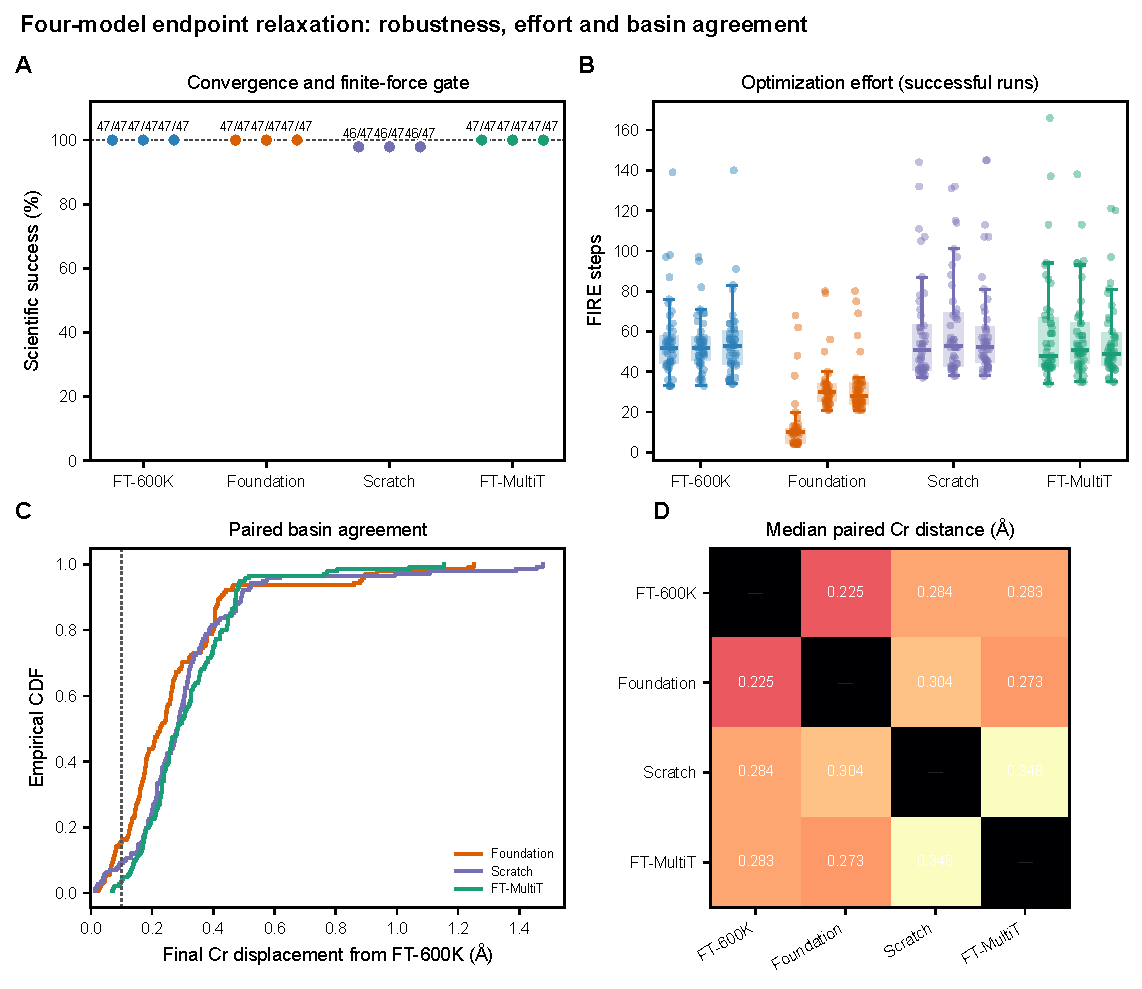
\includegraphics[width=\linewidth,height=0.42\textheight,keepaspectratio]{figure_pages/assets/fig_011.pdf}
\caption{Mace endpoint energy/force or relaxation comparison. This page shows the candidate output ``Fig1 endpoint robustness'' within the audited ENDPOINT-MACE family. The panel identity, source scope, and current status are retained in the accompanying evidence matrix.}
\label{fig:candidate_011}
\end{figure}
\textbf{Results text draft.} The figure compares endpoint behavior across the declared MACE model set and preserves the sampled endpoint identity. It is a local structural/energetic probe, not a transition-state calculation.
\textbf{Discussion and boundary.} Use to motivate model differences at endpoints, while keeping the separate path-level and DFT convergence limitations visible.
\textbf{Article placement.} Proposed article location: Results: endpoint robustness.
\textbf{Reviewer linkage:} overall status NO\_DIRECT\_REVIEWER\_FIGURE\_LINK.
No direct reviewer-response figure linkage was identified; this page is retained for scientific/article audit rather than as a direct reviewer response.
\textbf{Evidence pointers.}
\begin{itemize}[leftmargin=1.4em,noitemsep]
\item Data/processed: \begingroup\scriptsize\url{main/analysis/mace_endpoint_four_model/outputs/table_energy_span_by_endpoint.csv}\endgroup
\item Data/processed: \begingroup\scriptsize\url{main/analysis/mace_endpoint_four_model/outputs/table_model_agreement.csv}\endgroup
\item Plot/processing script: \begingroup\scriptsize\url{main/analysis/mace_endpoint_four_model/analyze_and_plot.py}\endgroup
\item Caption/text source: \begingroup\scriptsize\url{main/analysis/mace_endpoint_four_model/outputs/discussion_draft.md}\endgroup
\end{itemize}
\statusline{\textbf{Audit gap / next action:} Confirm current article section and whether endpoint task remains in the revision}
\vfill
\clearpage
\section{FIG-012 --- Fig2 relative energy landscape}
\label{figpage:fig-012}
\textbf{Group:} ENDPOINT-MACE\quad \textbf{Evidence chain:} traceable\quad \textbf{Status:} unclassified
\begin{figure}[H]
\centering
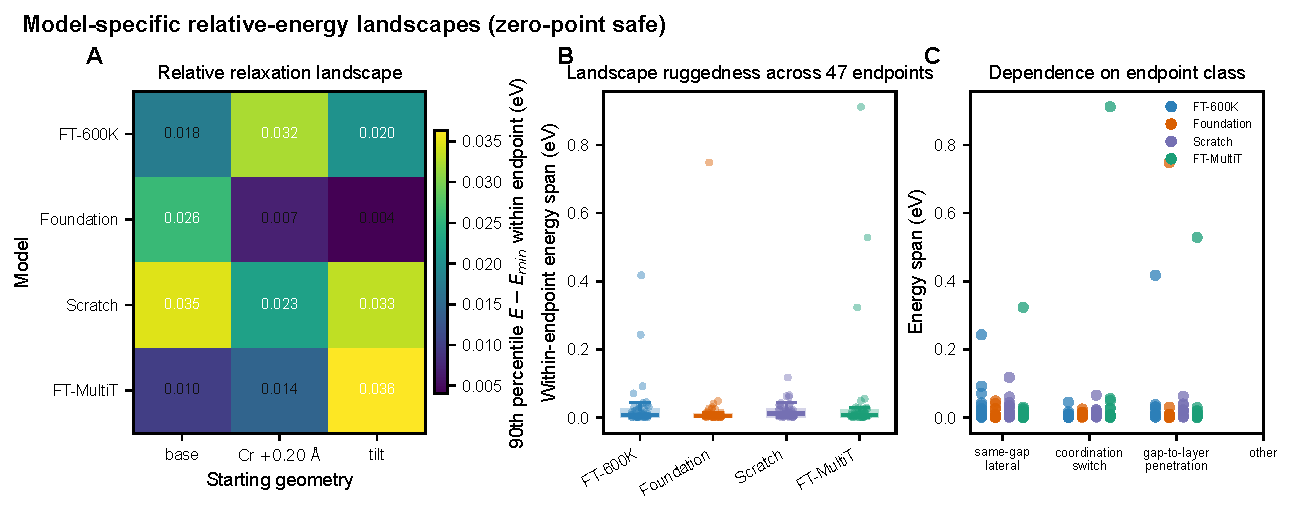
\includegraphics[width=\linewidth,height=0.42\textheight,keepaspectratio]{figure_pages/assets/fig_012.pdf}
\caption{Mace endpoint energy/force or relaxation comparison. This page shows the candidate output ``Fig2 relative energy landscape'' within the audited ENDPOINT-MACE family. The panel identity, source scope, and current status are retained in the accompanying evidence matrix.}
\label{fig:candidate_012}
\end{figure}
\textbf{Results text draft.} The figure compares endpoint behavior across the declared MACE model set and preserves the sampled endpoint identity. It is a local structural/energetic probe, not a transition-state calculation.
\textbf{Discussion and boundary.} Use to motivate model differences at endpoints, while keeping the separate path-level and DFT convergence limitations visible.
\textbf{Article placement.} Proposed article location: Results: endpoint robustness.
\textbf{Reviewer linkage:} overall status NO\_DIRECT\_REVIEWER\_FIGURE\_LINK.
No direct reviewer-response figure linkage was identified; this page is retained for scientific/article audit rather than as a direct reviewer response.
\textbf{Evidence pointers.}
\begin{itemize}[leftmargin=1.4em,noitemsep]
\item Data/processed: \begingroup\scriptsize\url{main/analysis/mace_endpoint_four_model/outputs/table_energy_span_by_endpoint.csv}\endgroup
\item Data/processed: \begingroup\scriptsize\url{main/analysis/mace_endpoint_four_model/outputs/table_model_agreement.csv}\endgroup
\item Plot/processing script: \begingroup\scriptsize\url{main/analysis/mace_endpoint_four_model/analyze_and_plot.py}\endgroup
\item Caption/text source: \begingroup\scriptsize\url{main/analysis/mace_endpoint_four_model/outputs/discussion_draft.md}\endgroup
\end{itemize}
\statusline{\textbf{Audit gap / next action:} Confirm current article section and whether endpoint task remains in the revision}
\vfill
\clearpage
\section{FIG-013 --- Time convergence}
\label{figpage:fig-013}
\textbf{Group:} MD-CONV\quad \textbf{Evidence chain:} partial\quad \textbf{Status:} unclassified
\begin{figure}[H]
\centering
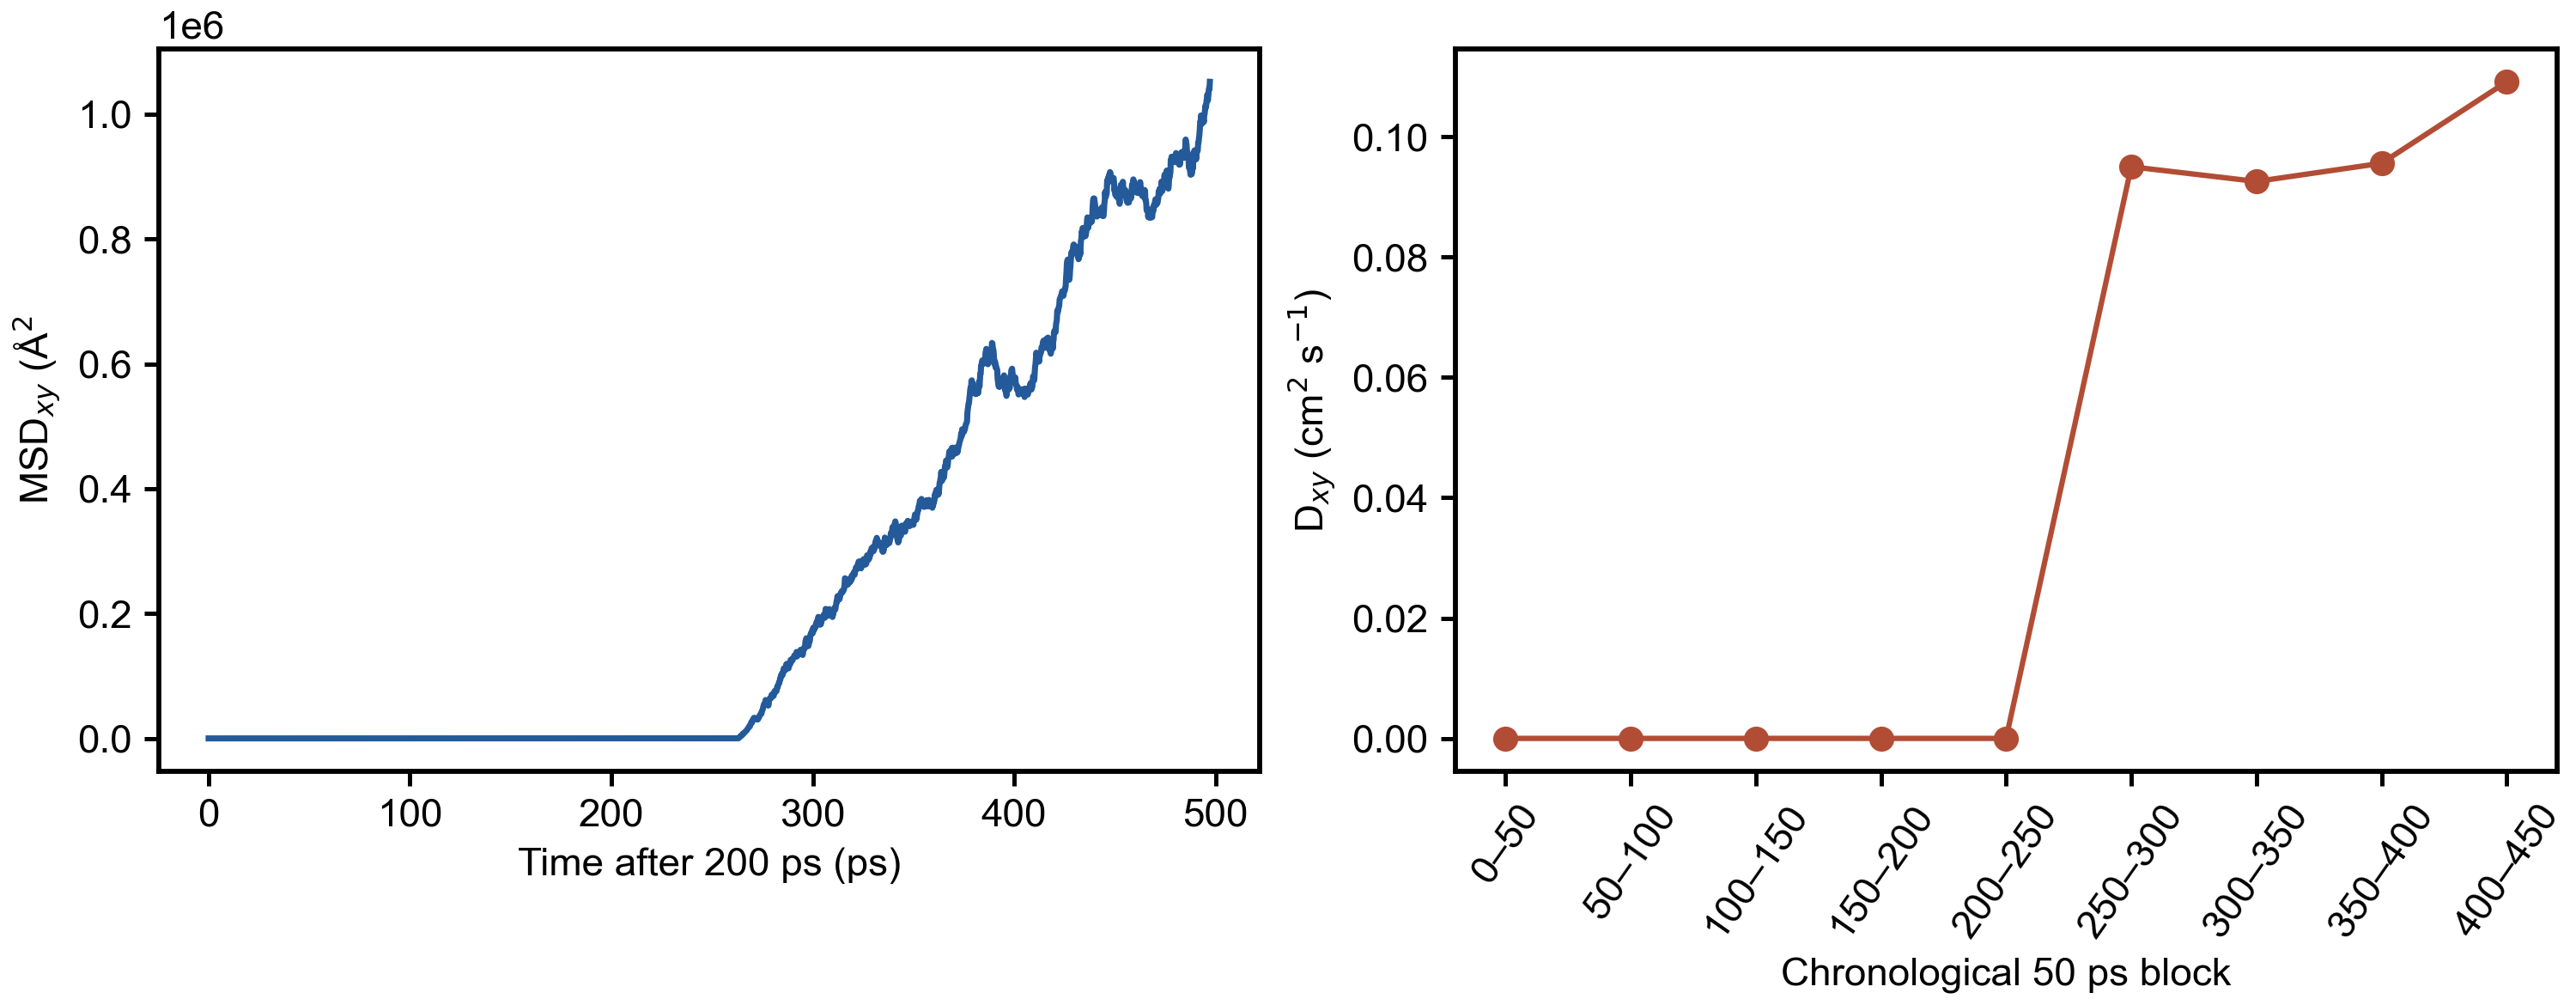
\includegraphics[width=\linewidth,height=0.42\textheight,keepaspectratio]{figure_pages/assets/fig_013.png}
\caption{Molecular-dynamics convergence, block statistics, or transport diagnostics. This page shows the candidate output ``Time convergence'' within the audited MD-CONV family. The panel identity, source scope, and current status are retained in the accompanying evidence matrix.}
\label{fig:candidate_013}
\end{figure}
\textbf{Results text draft.} The displayed curves or summaries show the convergence behavior and uncertainty treatment available in the corresponding source analysis. Only quantities backed by complete trajectories and the declared block protocol should enter manuscript ranking.
\textbf{Discussion and boundary.} Use for methods or SI validation. Short, mismatched, or provenance-only trajectories remain labeled as such and are excluded from formal cross-model conclusions.
\textbf{Article placement.} Proposed article location: SI transport-method validation.
\textbf{Reviewer linkage:} overall status PENDING.
\begin{itemize}[leftmargin=1.4em,noitemsep]
\item \textbf{REV-C9 (PENDING):} Resolve the asymmetric FT-600K MD transport protocol and its effect on D and kappa. \emph{Completed:} Legacy FT-600K transport values are quarantined and excluded from ranking; the figure can document that boundary. \emph{Still required:} Run the corrected matched-protocol FT-600K long trajectory, block-average D/kappa, and close the multi-seed uncertainty before reporting a final transport comparison.
\end{itemize}
\textbf{Evidence pointers.}
\begin{itemize}[leftmargin=1.4em,noitemsep]
\item Data/processed: \begingroup\scriptsize\url{main/analysis/mace_md_time_convergence_20261001/from-scratch/blocks_50ps.csv}\endgroup
\item Data/processed: \begingroup\scriptsize\url{main/analysis/mace_md_time_convergence_20261001/from-scratch/cumulative_windows.csv}\endgroup
\item Caption/text source: \begingroup\scriptsize\url{main/analysis/mace_md_time_convergence_20261001/REPORT.md}\endgroup
\end{itemize}
\statusline{\textbf{Audit gap / next action:} Plot script is not co-located with the image; map exact source generator}
\vfill
\clearpage
\section{FIG-014 --- Time convergence}
\label{figpage:fig-014}
\textbf{Group:} MD-CONV\quad \textbf{Evidence chain:} partial\quad \textbf{Status:} unclassified
\begin{figure}[H]
\centering
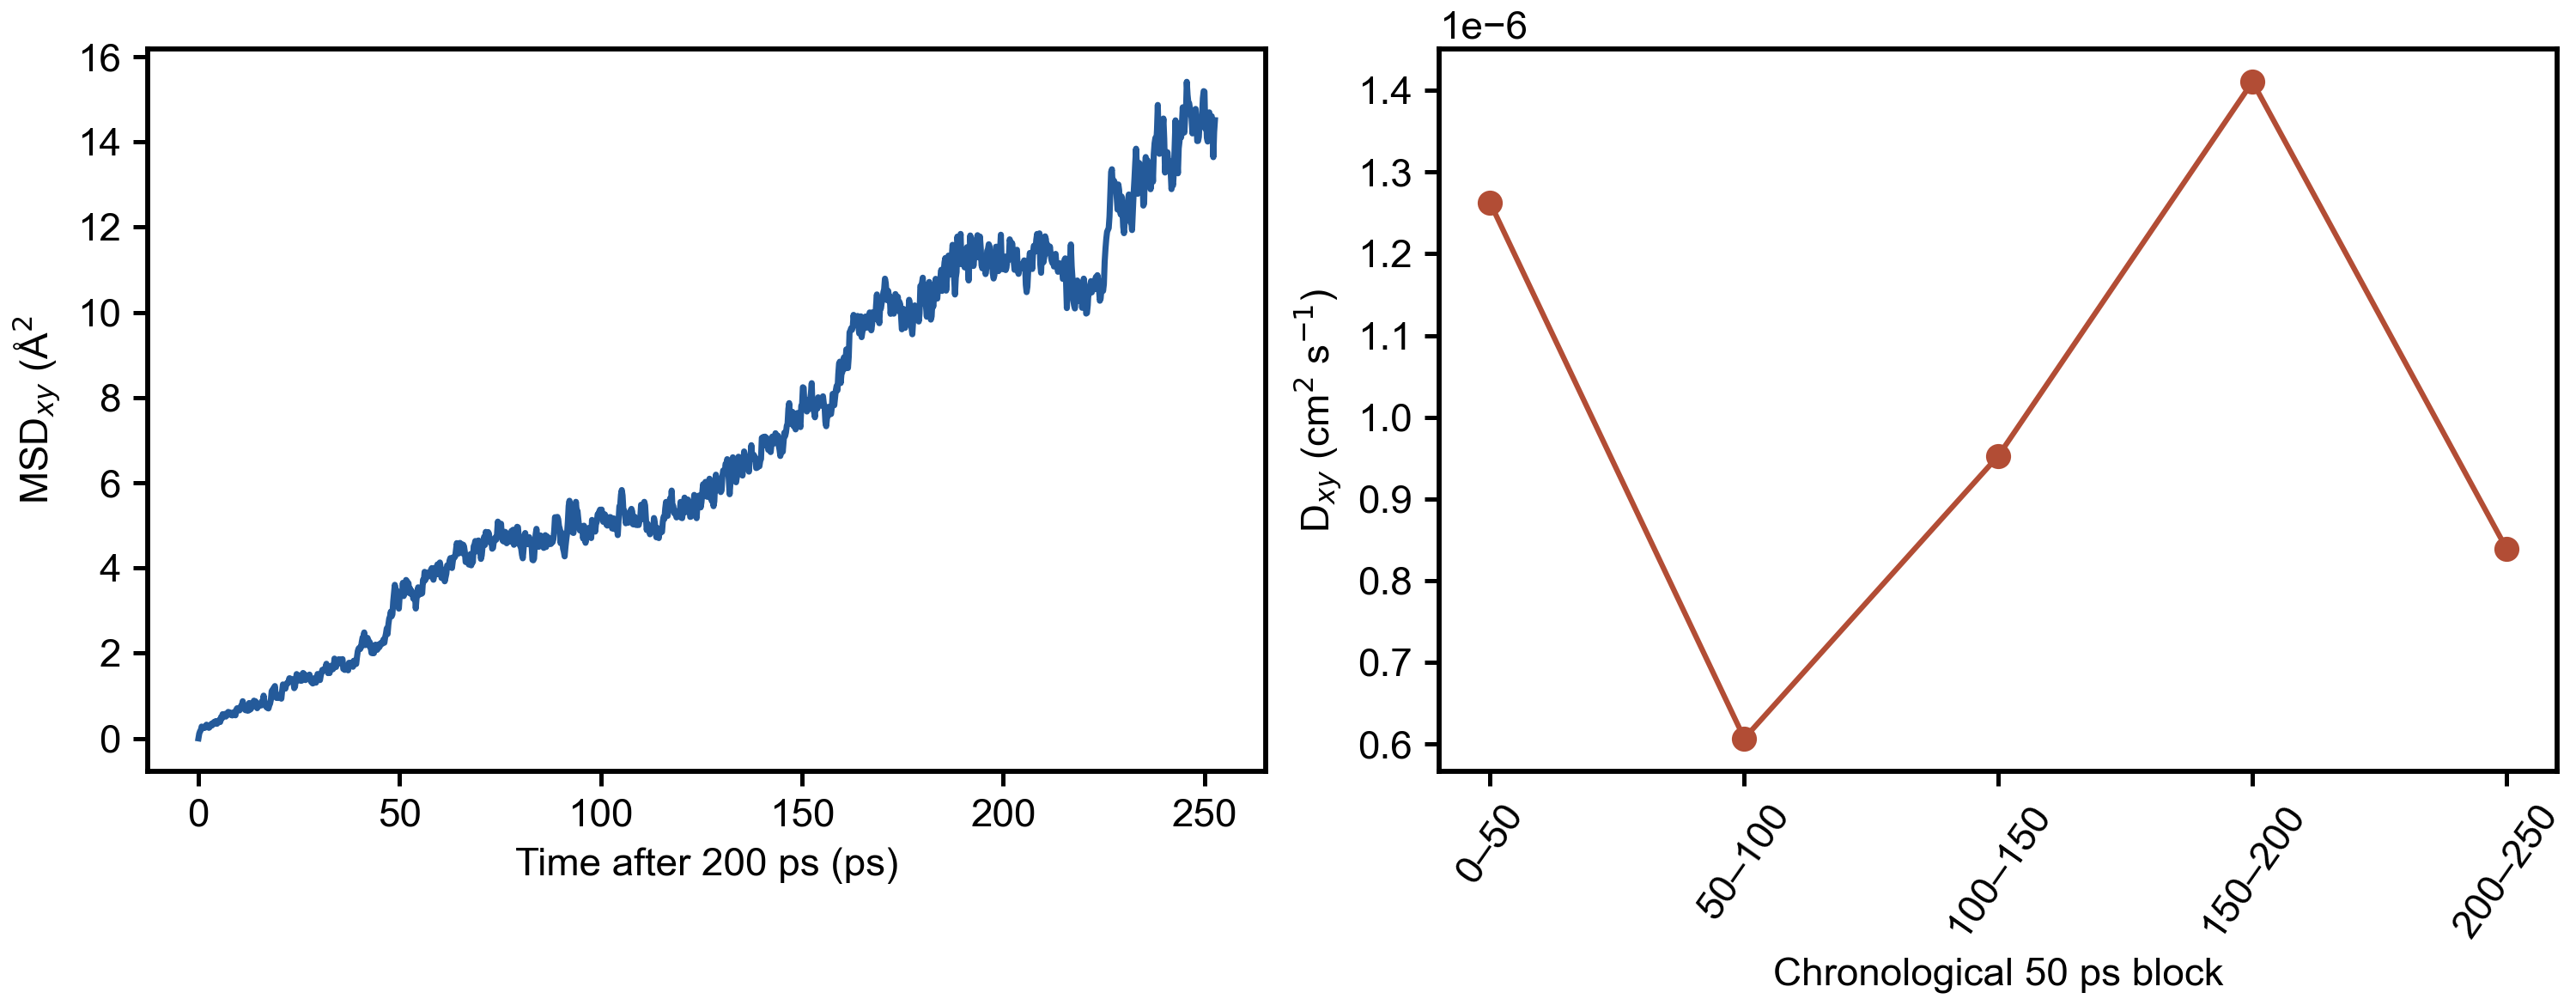
\includegraphics[width=\linewidth,height=0.42\textheight,keepaspectratio]{figure_pages/assets/fig_014.png}
\caption{Molecular-dynamics convergence, block statistics, or transport diagnostics. This page shows the candidate output ``Time convergence'' within the audited MD-CONV family. The panel identity, source scope, and current status are retained in the accompanying evidence matrix.}
\label{fig:candidate_014}
\end{figure}
\textbf{Results text draft.} The displayed curves or summaries show the convergence behavior and uncertainty treatment available in the corresponding source analysis. Only quantities backed by complete trajectories and the declared block protocol should enter manuscript ranking.
\textbf{Discussion and boundary.} Use for methods or SI validation. Short, mismatched, or provenance-only trajectories remain labeled as such and are excluded from formal cross-model conclusions.
\textbf{Article placement.} Proposed article location: SI transport-method validation.
\textbf{Reviewer linkage:} overall status PENDING.
\begin{itemize}[leftmargin=1.4em,noitemsep]
\item \textbf{REV-C9 (PENDING):} Resolve the asymmetric FT-600K MD transport protocol and its effect on D and kappa. \emph{Completed:} Legacy FT-600K transport values are quarantined and excluded from ranking; the figure can document that boundary. \emph{Still required:} Run the corrected matched-protocol FT-600K long trajectory, block-average D/kappa, and close the multi-seed uncertainty before reporting a final transport comparison.
\end{itemize}
\textbf{Evidence pointers.}
\begin{itemize}[leftmargin=1.4em,noitemsep]
\item Data/processed: \begingroup\scriptsize\url{main/analysis/mace_md_time_convergence_20261001/from_scratch_seg.tsv}\endgroup
\item Data/processed: \begingroup\scriptsize\url{main/analysis/mace_md_time_convergence_20261001/multi-T/blocks_50ps.csv}\endgroup
\item Caption/text source: \begingroup\scriptsize\url{main/analysis/mace_md_time_convergence_20261001/REPORT.md}\endgroup
\end{itemize}
\statusline{\textbf{Audit gap / next action:} Plot script is not co-located with the image; map exact source generator}
\vfill
\clearpage
\section{FIG-015 --- Fig1 force disagreement}
\label{figpage:fig-015}
\textbf{Group:} P1-FORCE\quad \textbf{Evidence chain:} traceable\quad \textbf{Status:} comparison
\begin{figure}[H]
\centering
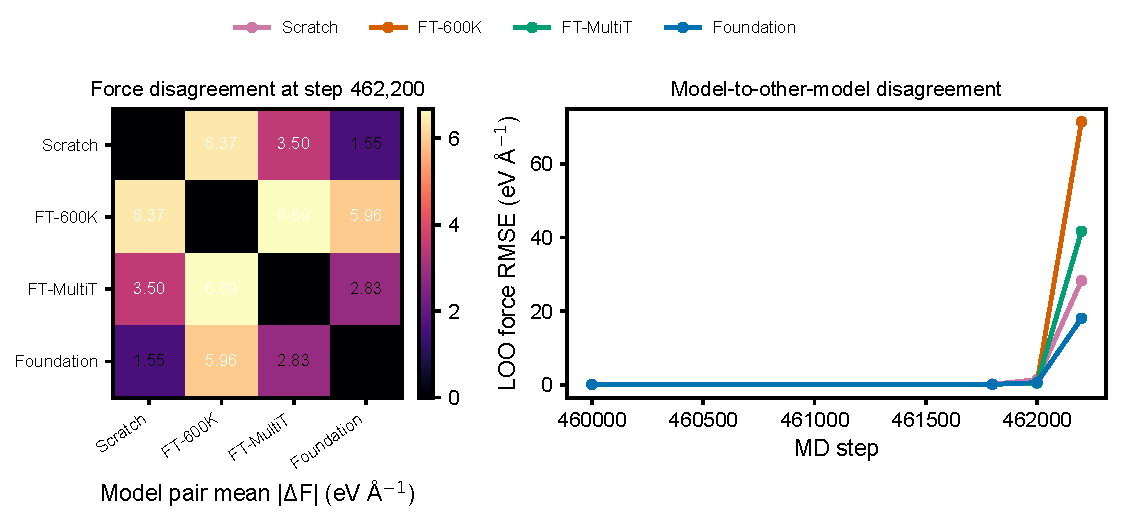
\includegraphics[width=\linewidth,height=0.42\textheight,keepaspectratio]{figure_pages/assets/fig_015.pdf}
\caption{Static force-disagreement and model-transfer diagnostics. This page shows the candidate output ``Fig1 force disagreement'' within the audited P1-FORCE family. The panel identity, source scope, and current status are retained in the accompanying evidence matrix.}
\label{fig:candidate_015}
\end{figure}
\textbf{Results text draft.} The figure compares model forces on a common set of configurations and exposes disagreement patterns that are not reducible to a single aggregate RMSE. The exact sampling scope and model provenance are retained in the evidence row.
\textbf{Discussion and boundary.} This supports the static-reference part of the benchmark. It does not by itself establish stability on a dynamically evolving path or agreement with converged DFT barriers.
\textbf{Article placement.} Proposed article location: Results: model disagreement and trajectory-integrity gate.
\textbf{Reviewer linkage:} overall status NO\_DIRECT\_REVIEWER\_FIGURE\_LINK.
No direct reviewer-response figure linkage was identified; this page is retained for scientific/article audit rather than as a direct reviewer response.
\textbf{Evidence pointers.}
\begin{itemize}[leftmargin=1.4em,noitemsep]
\item Data/processed: \begingroup\scriptsize\url{main/analysis/phase1_static_force_comparison_20261002/models_rockfish.json}\endgroup
\item Caption/text source: \begingroup\scriptsize\url{main/analysis/phase1_static_force_comparison_20261002/Methods.md}\endgroup
\item Caption/text source: \begingroup\scriptsize\url{main/analysis/phase1_static_force_comparison_20261002/README.md}\endgroup
\end{itemize}
\statusline{\textbf{Audit gap / next action:} Not yet integrated into the paper source}
\vfill
\clearpage
\section{FIG-016 --- Fig2 key local force}
\label{figpage:fig-016}
\textbf{Group:} P1-FORCE\quad \textbf{Evidence chain:} traceable\quad \textbf{Status:} comparison
\begin{figure}[H]
\centering
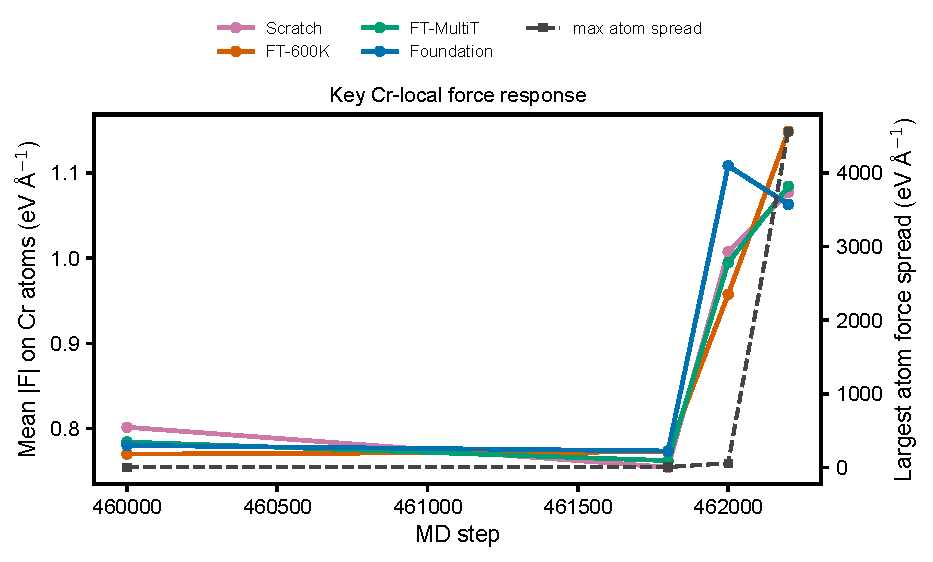
\includegraphics[width=\linewidth,height=0.42\textheight,keepaspectratio]{figure_pages/assets/fig_016.pdf}
\caption{Static force-disagreement and model-transfer diagnostics. This page shows the candidate output ``Fig2 key local force'' within the audited P1-FORCE family. The panel identity, source scope, and current status are retained in the accompanying evidence matrix.}
\label{fig:candidate_016}
\end{figure}
\textbf{Results text draft.} The figure compares model forces on a common set of configurations and exposes disagreement patterns that are not reducible to a single aggregate RMSE. The exact sampling scope and model provenance are retained in the evidence row.
\textbf{Discussion and boundary.} This supports the static-reference part of the benchmark. It does not by itself establish stability on a dynamically evolving path or agreement with converged DFT barriers.
\textbf{Article placement.} Proposed article location: Results: model disagreement and trajectory-integrity gate.
\textbf{Reviewer linkage:} overall status NO\_DIRECT\_REVIEWER\_FIGURE\_LINK.
No direct reviewer-response figure linkage was identified; this page is retained for scientific/article audit rather than as a direct reviewer response.
\textbf{Evidence pointers.}
\begin{itemize}[leftmargin=1.4em,noitemsep]
\item Data/processed: \begingroup\scriptsize\url{main/analysis/phase1_static_force_comparison_20261002/models_rockfish.json}\endgroup
\item Caption/text source: \begingroup\scriptsize\url{main/analysis/phase1_static_force_comparison_20261002/Methods.md}\endgroup
\item Caption/text source: \begingroup\scriptsize\url{main/analysis/phase1_static_force_comparison_20261002/README.md}\endgroup
\end{itemize}
\statusline{\textbf{Audit gap / next action:} Not yet integrated into the paper source}
\vfill
\clearpage
\section{FIG-017 --- Fig3 geometry step diagnostics}
\label{figpage:fig-017}
\textbf{Group:} P1-FORCE\quad \textbf{Evidence chain:} traceable\quad \textbf{Status:} exploratory;comparison
\begin{figure}[H]
\centering
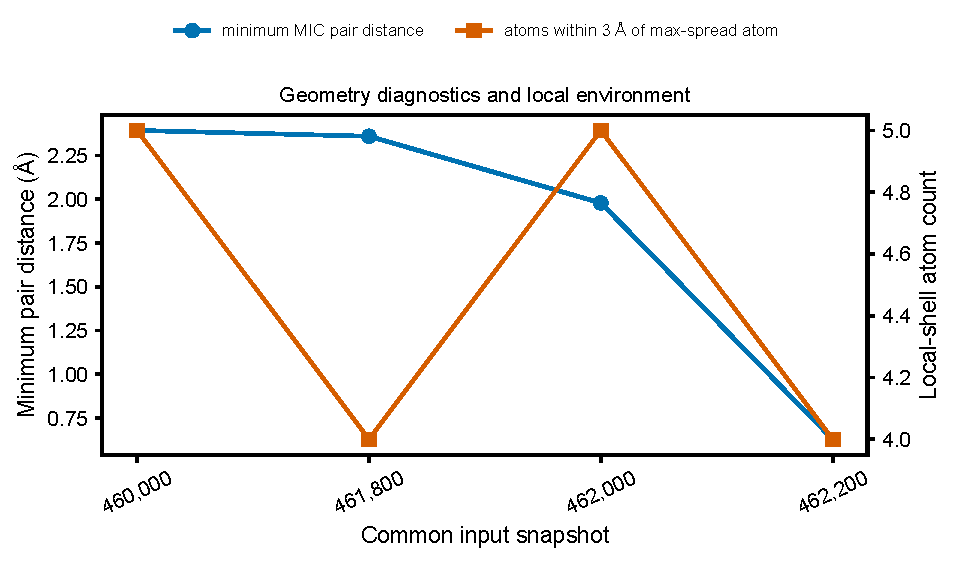
\includegraphics[width=\linewidth,height=0.42\textheight,keepaspectratio]{figure_pages/assets/fig_017.pdf}
\caption{Static force-disagreement and model-transfer diagnostics. This page shows the candidate output ``Fig3 geometry step diagnostics'' within the audited P1-FORCE family. The panel identity, source scope, and current status are retained in the accompanying evidence matrix.}
\label{fig:candidate_017}
\end{figure}
\textbf{Results text draft.} The figure compares model forces on a common set of configurations and exposes disagreement patterns that are not reducible to a single aggregate RMSE. The exact sampling scope and model provenance are retained in the evidence row.
\textbf{Discussion and boundary.} This supports the static-reference part of the benchmark. It does not by itself establish stability on a dynamically evolving path or agreement with converged DFT barriers.
\textbf{Article placement.} Proposed article location: Results: model disagreement and trajectory-integrity gate.
\textbf{Reviewer linkage:} overall status NO\_DIRECT\_REVIEWER\_FIGURE\_LINK.
No direct reviewer-response figure linkage was identified; this page is retained for scientific/article audit rather than as a direct reviewer response.
\textbf{Evidence pointers.}
\begin{itemize}[leftmargin=1.4em,noitemsep]
\item Data/processed: \begingroup\scriptsize\url{main/analysis/phase1_static_force_comparison_20261002/models_rockfish.json}\endgroup
\item Caption/text source: \begingroup\scriptsize\url{main/analysis/phase1_static_force_comparison_20261002/Methods.md}\endgroup
\item Caption/text source: \begingroup\scriptsize\url{main/analysis/phase1_static_force_comparison_20261002/README.md}\endgroup
\end{itemize}
\statusline{\textbf{Audit gap / next action:} Not yet integrated into the paper source}
\vfill
\clearpage
\section{FIG-018 --- Phase2 handoff timeseries}
\label{figpage:fig-018}
\textbf{Group:} P2-HANDOFF\quad \textbf{Evidence chain:} traceable\quad \textbf{Status:} audit
\begin{figure}[H]
\centering
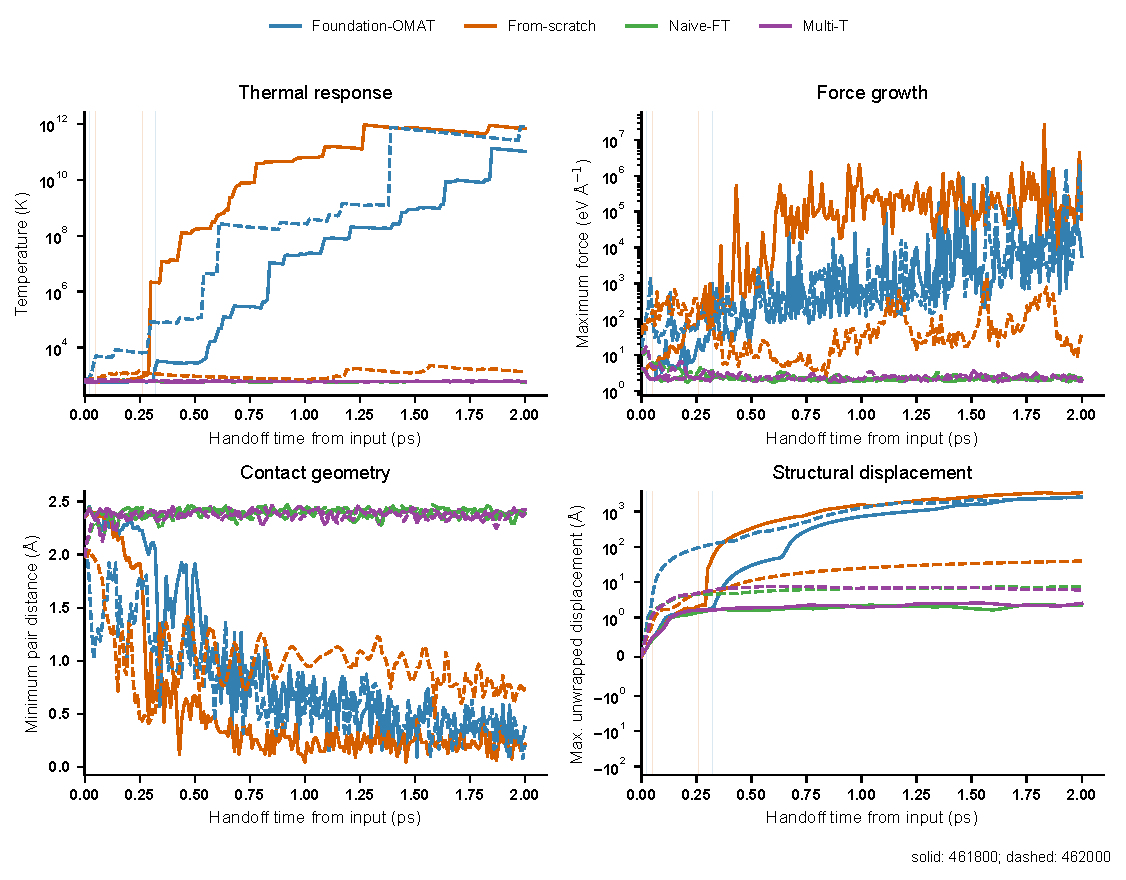
\includegraphics[width=\linewidth,height=0.42\textheight,keepaspectratio]{figure_pages/assets/fig_018.pdf}
\caption{Handoff molecular-dynamics diagnostics and first-divergence audit. This page shows the candidate output ``Phase2 handoff timeseries'' within the audited P2-HANDOFF family. The panel identity, source scope, and current status are retained in the accompanying evidence matrix.}
\label{fig:candidate_018}
\end{figure}
\textbf{Results text draft.} The panels track the temperature, force, contact, and structural observables used to locate the first anomalous behavior after protocol handoff. Run-level integrity and local-neighborhood evidence are kept alongside the visualization.
\textbf{Discussion and boundary.} This is a diagnostic figure for identifying when and how trajectories depart from the accepted regime. It is not a replacement for a completed, gate-passing production trajectory.
\textbf{Article placement.} Proposed article location: Results: dynamic stability mechanism; possibly SI.
\textbf{Reviewer linkage:} overall status NO\_DIRECT\_REVIEWER\_FIGURE\_LINK.
No direct reviewer-response figure linkage was identified; this page is retained for scientific/article audit rather than as a direct reviewer response.
\textbf{Evidence pointers.}
\begin{itemize}[leftmargin=1.4em,noitemsep]
\item Data/processed: \begingroup\scriptsize\url{main/analysis/phase2_handoff_md_20261002/audit_20261003/figures/figure_manifest.json}\endgroup
\item Data/processed: \begingroup\scriptsize\url{main/analysis/phase2_handoff_md_20261002/audit_20261003/figures/plot_env.json}\endgroup
\item Plot/processing script: \begingroup\scriptsize\url{main/analysis/phase2_handoff_md_20261002/audit_20261003/audit_phase2.py}\endgroup
\item Plot/processing script: \begingroup\scriptsize\url{main/analysis/phase2_handoff_md_20261002/audit_20261003/extract_first_anomaly_remote.py}\endgroup
\item Caption/text source: \begingroup\scriptsize\url{main/analysis/phase2_handoff_md_20261002/audit_20261003/PAPER_TEXT.md}\endgroup
\item Caption/text source: \begingroup\scriptsize\url{main/analysis/phase2_handoff_md_20261002/audit_20261003/README.md}\endgroup
\end{itemize}
\statusline{\textbf{Audit gap / next action:} Keep duplicate retry/audit renders linked and designate one canonical output}
\vfill
\clearpage
\section{FIG-019 --- Phase2 stability gate}
\label{figpage:fig-019}
\textbf{Group:} P2-HANDOFF\quad \textbf{Evidence chain:} traceable\quad \textbf{Status:} audit
\begin{figure}[H]
\centering
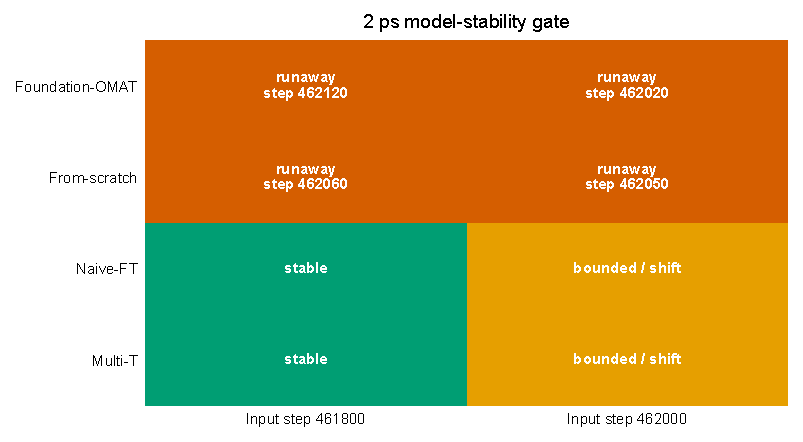
\includegraphics[width=\linewidth,height=0.42\textheight,keepaspectratio]{figure_pages/assets/fig_019.pdf}
\caption{Handoff molecular-dynamics diagnostics and first-divergence audit. This page shows the candidate output ``Phase2 stability gate'' within the audited P2-HANDOFF family. The panel identity, source scope, and current status are retained in the accompanying evidence matrix.}
\label{fig:candidate_019}
\end{figure}
\textbf{Results text draft.} The panels track the temperature, force, contact, and structural observables used to locate the first anomalous behavior after protocol handoff. Run-level integrity and local-neighborhood evidence are kept alongside the visualization.
\textbf{Discussion and boundary.} This is a diagnostic figure for identifying when and how trajectories depart from the accepted regime. It is not a replacement for a completed, gate-passing production trajectory.
\textbf{Article placement.} Proposed article location: Results: dynamic stability mechanism; possibly SI.
\textbf{Reviewer linkage:} overall status NO\_DIRECT\_REVIEWER\_FIGURE\_LINK.
No direct reviewer-response figure linkage was identified; this page is retained for scientific/article audit rather than as a direct reviewer response.
\textbf{Evidence pointers.}
\begin{itemize}[leftmargin=1.4em,noitemsep]
\item Data/processed: \begingroup\scriptsize\url{main/analysis/phase2_handoff_md_20261002/audit_20261003/figures/figure_manifest.json}\endgroup
\item Data/processed: \begingroup\scriptsize\url{main/analysis/phase2_handoff_md_20261002/audit_20261003/figures/plot_env.json}\endgroup
\item Plot/processing script: \begingroup\scriptsize\url{main/analysis/phase2_handoff_md_20261002/audit_20261003/audit_phase2.py}\endgroup
\item Plot/processing script: \begingroup\scriptsize\url{main/analysis/phase2_handoff_md_20261002/audit_20261003/extract_first_anomaly_remote.py}\endgroup
\item Caption/text source: \begingroup\scriptsize\url{main/analysis/phase2_handoff_md_20261002/audit_20261003/PAPER_TEXT.md}\endgroup
\item Caption/text source: \begingroup\scriptsize\url{main/analysis/phase2_handoff_md_20261002/audit_20261003/README.md}\endgroup
\end{itemize}
\statusline{\textbf{Audit gap / next action:} Keep duplicate retry/audit renders linked and designate one canonical output}
\vfill
\clearpage
\section{FIG-020 --- Handoff stability heatmap}
\label{figpage:fig-020}
\textbf{Group:} P2-HANDOFF\quad \textbf{Evidence chain:} traceable\quad \textbf{Status:} unclassified
\begin{figure}[H]
\centering
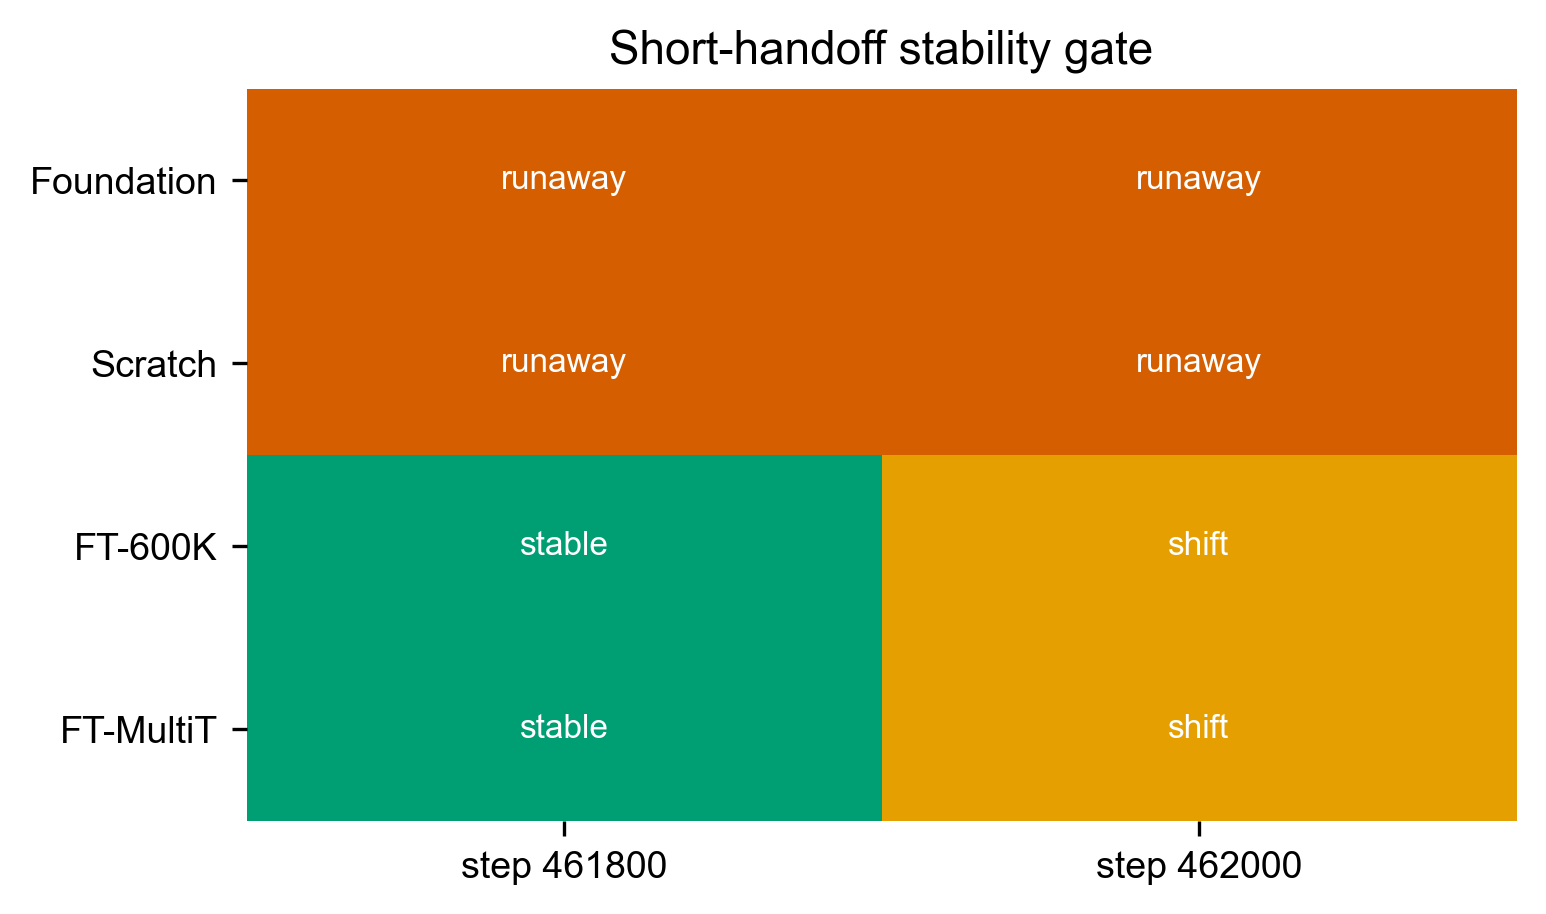
\includegraphics[width=\linewidth,height=0.42\textheight,keepaspectratio]{figure_pages/assets/fig_020.png}
\caption{Handoff molecular-dynamics diagnostics and first-divergence audit. This page shows the candidate output ``Handoff stability heatmap'' within the audited P2-HANDOFF family. The panel identity, source scope, and current status are retained in the accompanying evidence matrix.}
\label{fig:candidate_020}
\end{figure}
\textbf{Results text draft.} The panels track the temperature, force, contact, and structural observables used to locate the first anomalous behavior after protocol handoff. Run-level integrity and local-neighborhood evidence are kept alongside the visualization.
\textbf{Discussion and boundary.} This is a diagnostic figure for identifying when and how trajectories depart from the accepted regime. It is not a replacement for a completed, gate-passing production trajectory.
\textbf{Article placement.} Proposed article location: Results: dynamic stability mechanism; possibly SI.
\textbf{Reviewer linkage:} overall status NO\_DIRECT\_REVIEWER\_FIGURE\_LINK.
No direct reviewer-response figure linkage was identified; this page is retained for scientific/article audit rather than as a direct reviewer response.
\textbf{Evidence pointers.}
\begin{itemize}[leftmargin=1.4em,noitemsep]
\item Data/processed: \begingroup\scriptsize\url{main/analysis/phase2_handoff_md_20261002/remote_artifacts/runs/retry2/stability_summary.csv}\endgroup
\item Data/processed: \begingroup\scriptsize\url{main/analysis/phase2_handoff_md_20261002/remote_artifacts/runs/retry2/stability_summary.json}\endgroup
\end{itemize}
\statusline{\textbf{Audit gap / next action:} Keep duplicate retry/audit renders linked and designate one canonical output}
\vfill
\clearpage
\section{FIG-021 --- Handoff timeseries}
\label{figpage:fig-021}
\textbf{Group:} P2-HANDOFF\quad \textbf{Evidence chain:} traceable\quad \textbf{Status:} unclassified
\begin{figure}[H]
\centering
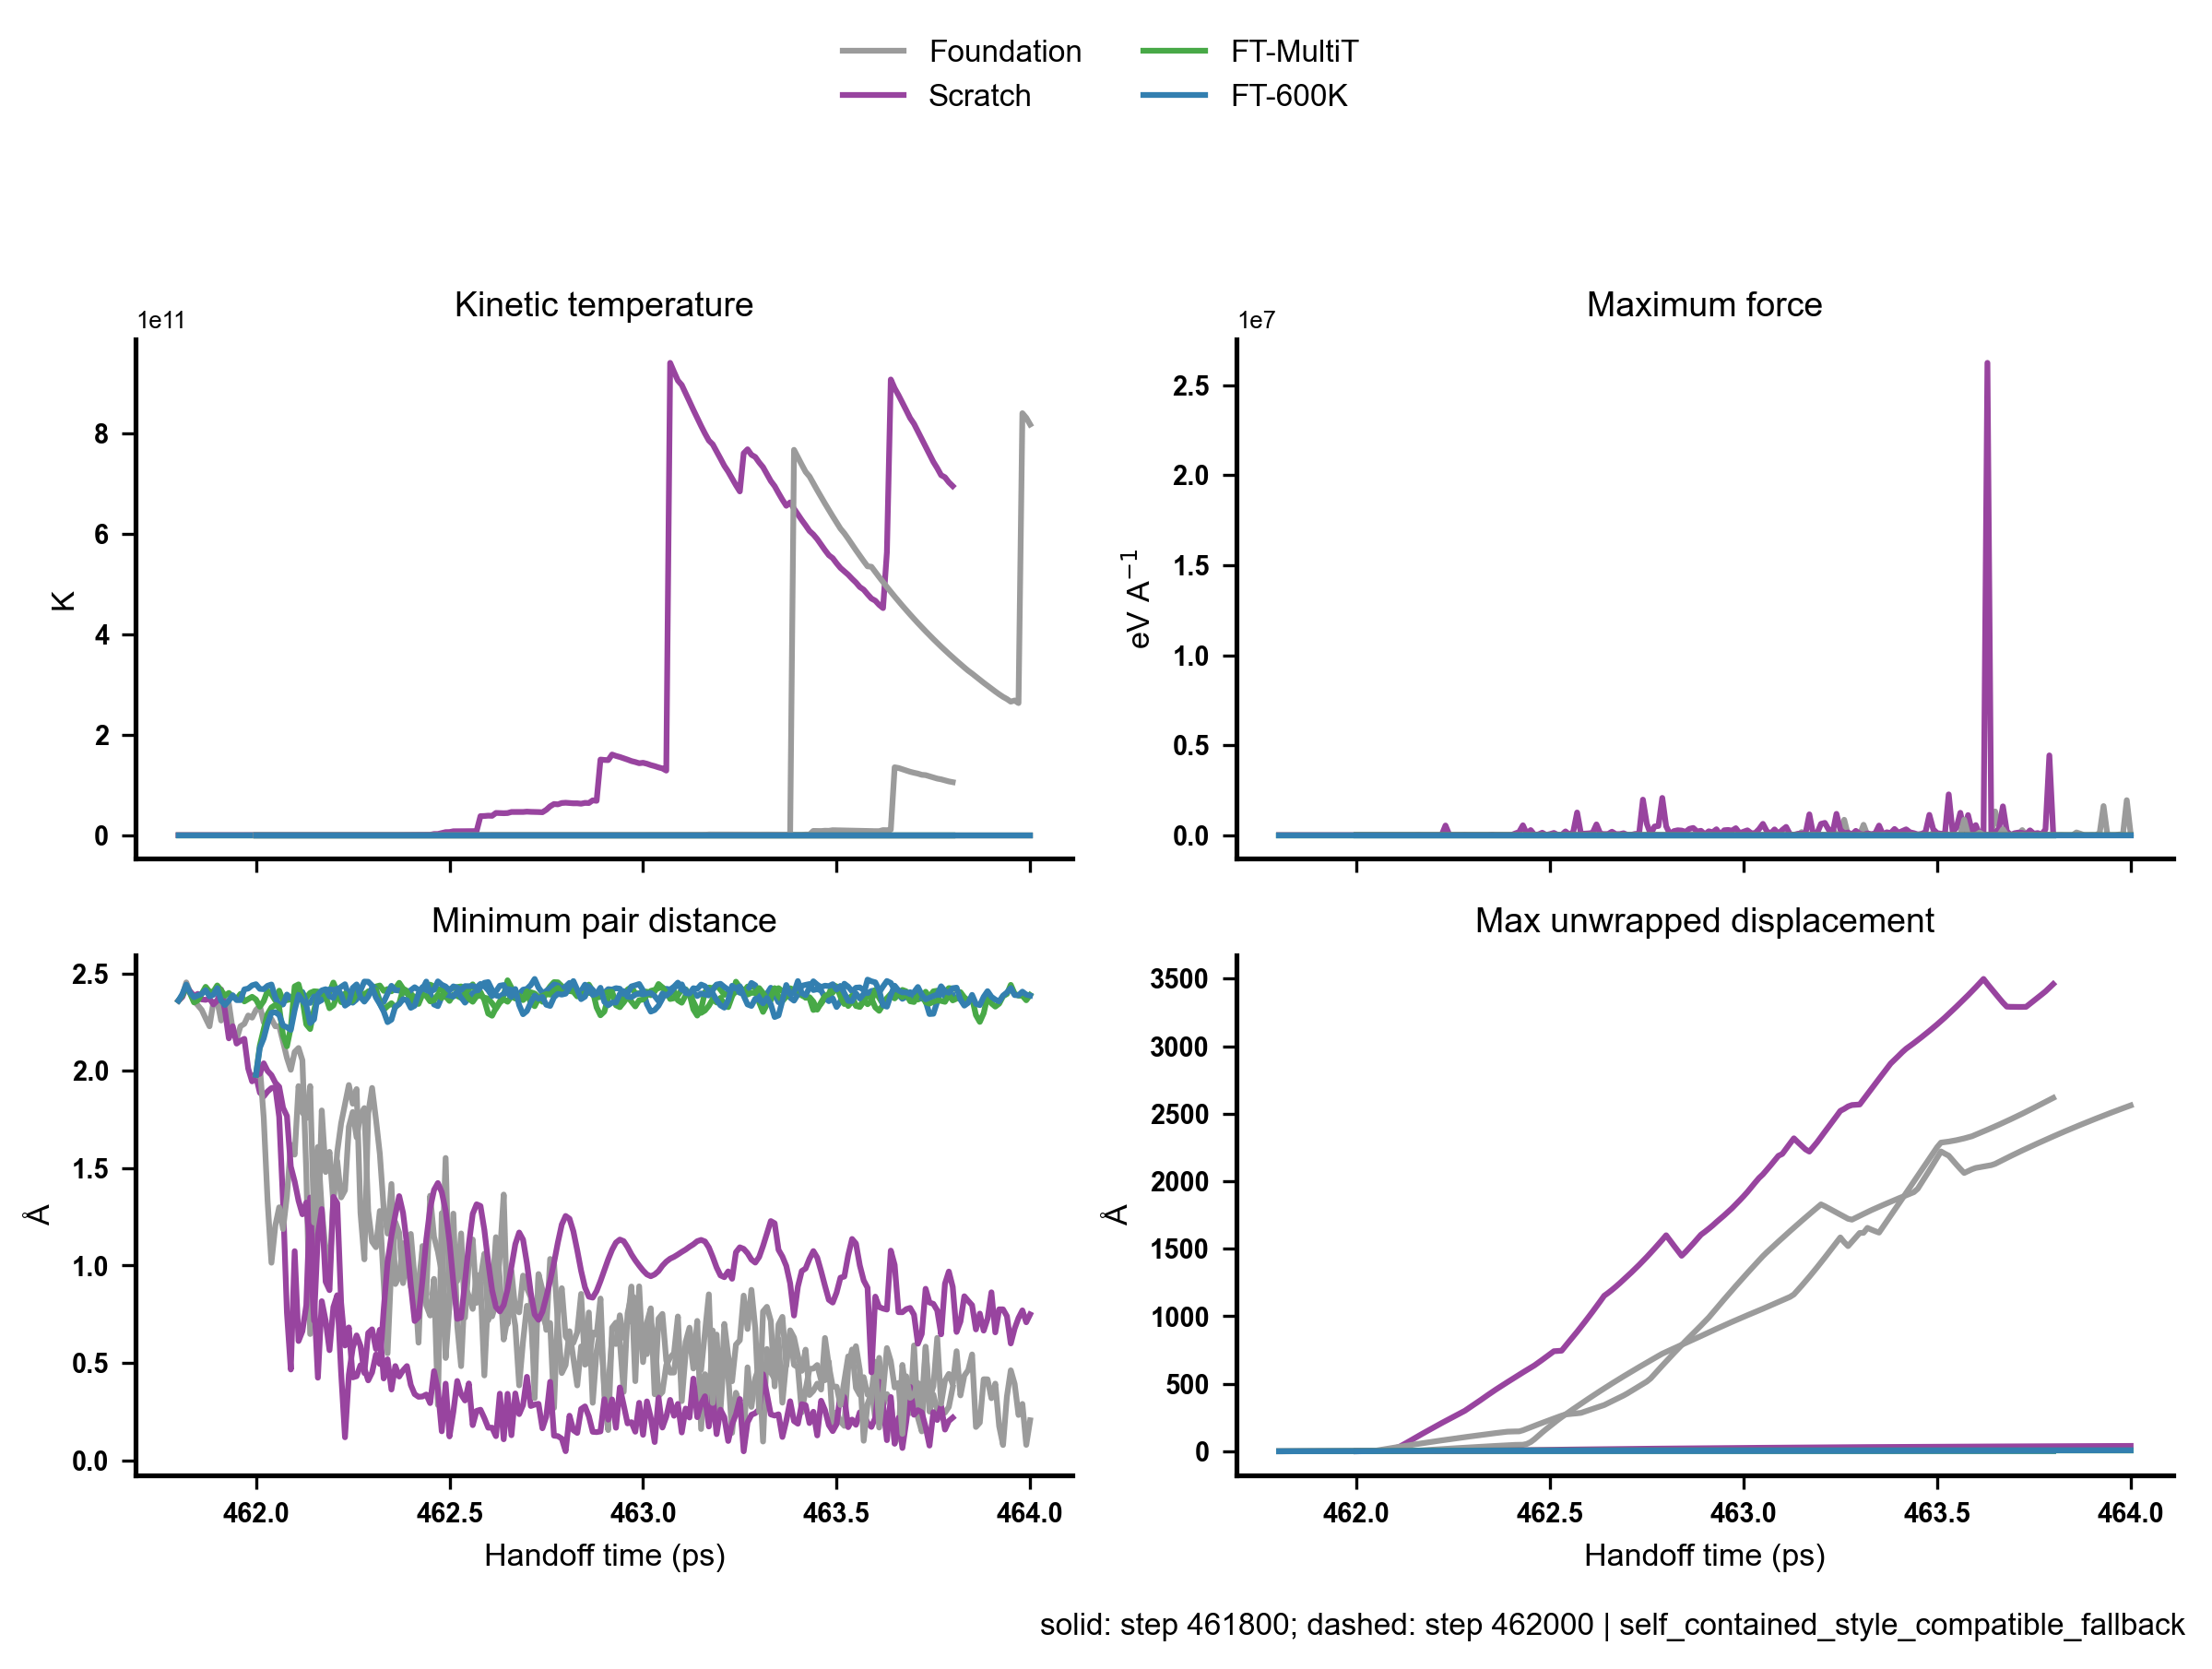
\includegraphics[width=\linewidth,height=0.42\textheight,keepaspectratio]{figure_pages/assets/fig_021.png}
\caption{Handoff molecular-dynamics diagnostics and first-divergence audit. This page shows the candidate output ``Handoff timeseries'' within the audited P2-HANDOFF family. The panel identity, source scope, and current status are retained in the accompanying evidence matrix.}
\label{fig:candidate_021}
\end{figure}
\textbf{Results text draft.} The panels track the temperature, force, contact, and structural observables used to locate the first anomalous behavior after protocol handoff. Run-level integrity and local-neighborhood evidence are kept alongside the visualization.
\textbf{Discussion and boundary.} This is a diagnostic figure for identifying when and how trajectories depart from the accepted regime. It is not a replacement for a completed, gate-passing production trajectory.
\textbf{Article placement.} Proposed article location: Results: dynamic stability mechanism; possibly SI.
\textbf{Reviewer linkage:} overall status NO\_DIRECT\_REVIEWER\_FIGURE\_LINK.
No direct reviewer-response figure linkage was identified; this page is retained for scientific/article audit rather than as a direct reviewer response.
\textbf{Evidence pointers.}
\begin{itemize}[leftmargin=1.4em,noitemsep]
\item Data/processed: \begingroup\scriptsize\url{main/analysis/phase2_handoff_md_20261002/remote_artifacts/runs/retry2/stability_summary.csv}\endgroup
\item Data/processed: \begingroup\scriptsize\url{main/analysis/phase2_handoff_md_20261002/remote_artifacts/runs/retry2/stability_summary.json}\endgroup
\end{itemize}
\statusline{\textbf{Audit gap / next action:} Keep duplicate retry/audit renders linked and designate one canonical output}
\vfill
\clearpage
\section{FIG-022 --- Phase2 handoff timeseries}
\label{figpage:fig-022}
\textbf{Group:} P2-HANDOFF\quad \textbf{Evidence chain:} traceable\quad \textbf{Status:} unclassified
\begin{figure}[H]
\centering
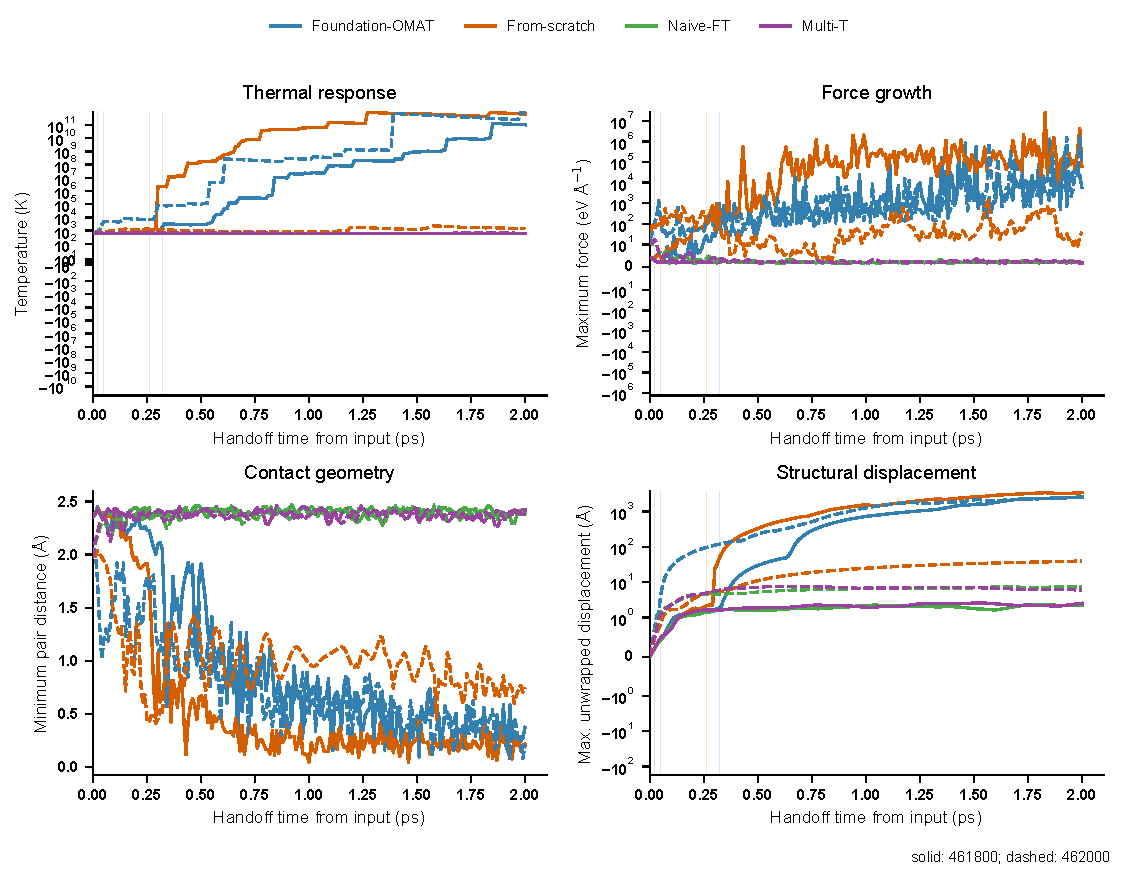
\includegraphics[width=\linewidth,height=0.42\textheight,keepaspectratio]{figure_pages/assets/fig_022.pdf}
\caption{Handoff molecular-dynamics diagnostics and first-divergence audit. This page shows the candidate output ``Phase2 handoff timeseries'' within the audited P2-HANDOFF family. The panel identity, source scope, and current status are retained in the accompanying evidence matrix.}
\label{fig:candidate_022}
\end{figure}
\textbf{Results text draft.} The panels track the temperature, force, contact, and structural observables used to locate the first anomalous behavior after protocol handoff. Run-level integrity and local-neighborhood evidence are kept alongside the visualization.
\textbf{Discussion and boundary.} This is a diagnostic figure for identifying when and how trajectories depart from the accepted regime. It is not a replacement for a completed, gate-passing production trajectory.
\textbf{Article placement.} Proposed article location: Results: dynamic stability mechanism; possibly SI.
\textbf{Reviewer linkage:} overall status NO\_DIRECT\_REVIEWER\_FIGURE\_LINK.
No direct reviewer-response figure linkage was identified; this page is retained for scientific/article audit rather than as a direct reviewer response.
\textbf{Evidence pointers.}
\begin{itemize}[leftmargin=1.4em,noitemsep]
\item Data/processed: \begingroup\scriptsize\url{main/analysis/phase2_handoff_md_20261003/figures/figure_manifest.json}\endgroup
\item Data/processed: \begingroup\scriptsize\url{main/analysis/phase2_handoff_md_20261003/figures/plot_env.json}\endgroup
\end{itemize}
\statusline{\textbf{Audit gap / next action:} Keep duplicate retry/audit renders linked and designate one canonical output}
\vfill
\clearpage
\section{FIG-023 --- Phase2 stability gate}
\label{figpage:fig-023}
\textbf{Group:} P2-HANDOFF\quad \textbf{Evidence chain:} traceable\quad \textbf{Status:} audit
\begin{figure}[H]
\centering
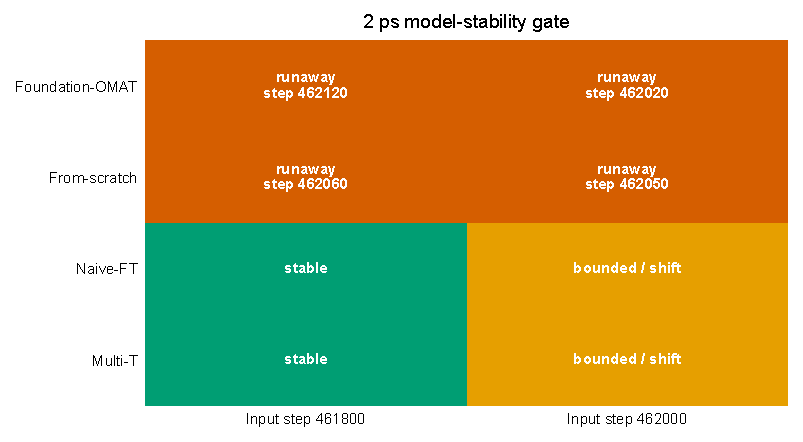
\includegraphics[width=\linewidth,height=0.42\textheight,keepaspectratio]{figure_pages/assets/fig_023.pdf}
\caption{Handoff molecular-dynamics diagnostics and first-divergence audit. This page shows the candidate output ``Phase2 stability gate'' within the audited P2-HANDOFF family. The panel identity, source scope, and current status are retained in the accompanying evidence matrix.}
\label{fig:candidate_023}
\end{figure}
\textbf{Results text draft.} The panels track the temperature, force, contact, and structural observables used to locate the first anomalous behavior after protocol handoff. Run-level integrity and local-neighborhood evidence are kept alongside the visualization.
\textbf{Discussion and boundary.} This is a diagnostic figure for identifying when and how trajectories depart from the accepted regime. It is not a replacement for a completed, gate-passing production trajectory.
\textbf{Article placement.} Proposed article location: Results: dynamic stability mechanism; possibly SI.
\textbf{Reviewer linkage:} overall status NO\_DIRECT\_REVIEWER\_FIGURE\_LINK.
No direct reviewer-response figure linkage was identified; this page is retained for scientific/article audit rather than as a direct reviewer response.
\textbf{Evidence pointers.}
\begin{itemize}[leftmargin=1.4em,noitemsep]
\item Data/processed: \begingroup\scriptsize\url{main/analysis/phase2_handoff_md_20261003/figures/figure_manifest.json}\endgroup
\item Data/processed: \begingroup\scriptsize\url{main/analysis/phase2_handoff_md_20261003/figures/plot_env.json}\endgroup
\end{itemize}
\statusline{\textbf{Audit gap / next action:} Keep duplicate retry/audit renders linked and designate one canonical output}
\vfill
\clearpage
\section{FIG-024 --- Placeholder dft gate status}
\label{figpage:fig-024}
\textbf{Group:} TASK2-ROSTER\quad \textbf{Evidence chain:} traceable\quad \textbf{Status:} placeholder
\begin{figure}[H]
\centering
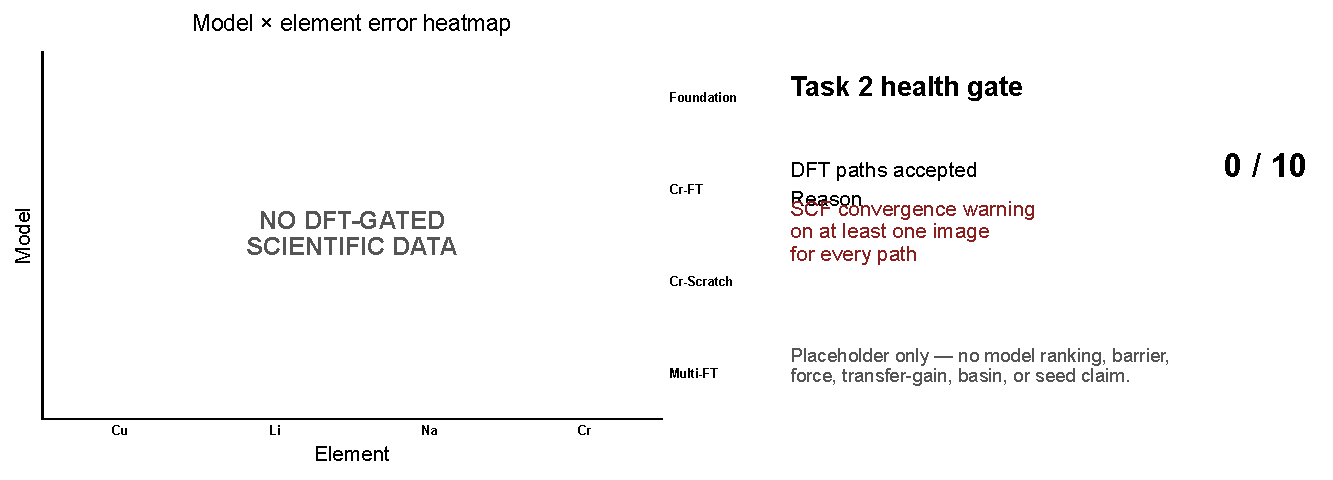
\includegraphics[width=\linewidth,height=0.42\textheight,keepaspectratio]{figure_pages/assets/fig_024.pdf}
\caption{Cross-element or multi-seed benchmark roster and pathway diagnostics. This page shows the candidate output ``Placeholder dft gate status'' within the audited TASK2-ROSTER family. The panel identity, source scope, and current status are retained in the accompanying evidence matrix.}
\label{fig:candidate_024}
\end{figure}
\textbf{Results text draft.} The figure organizes the evaluated systems, seeds, models, or pathway families so that coverage and missing cells are visible. Provisional and audited rows are not pooled when their protocols or provenance differ.
\textbf{Discussion and boundary.} This is appropriate for SI coverage and provenance discussion. It should not be read as a single uncertainty distribution across model-level and path-level variation.
\textbf{Article placement.} Proposed article location: Results: cross-element transfer and seed stability.
\textbf{Reviewer linkage:} overall status NO\_DIRECT\_REVIEWER\_FIGURE\_LINK.
No direct reviewer-response figure linkage was identified; this page is retained for scientific/article audit rather than as a direct reviewer response.
\textbf{Evidence pointers.}
\begin{itemize}[leftmargin=1.4em,noitemsep]
\item Caption/text source: \begingroup\scriptsize\url{main/analysis/task2_cross_element/HEALTH_GATE_REPORT.md}\endgroup
\item Caption/text source: \begingroup\scriptsize\url{main/analysis/task2_cross_element/figures/provisional_task2_neb_model_profiles_9panel.metadata.txt}\endgroup
\end{itemize}
\statusline{\textbf{Audit gap / next action:} DFT gate is still open; do not write barrier-accuracy claims}
\vfill
\clearpage
\section{FIG-025 --- Provisional task2 neb model profiles 9panel}
\label{figpage:fig-025}
\textbf{Group:} TASK2-ROSTER\quad \textbf{Evidence chain:} traceable\quad \textbf{Status:} provisional;comparison
\begin{figure}[H]
\centering
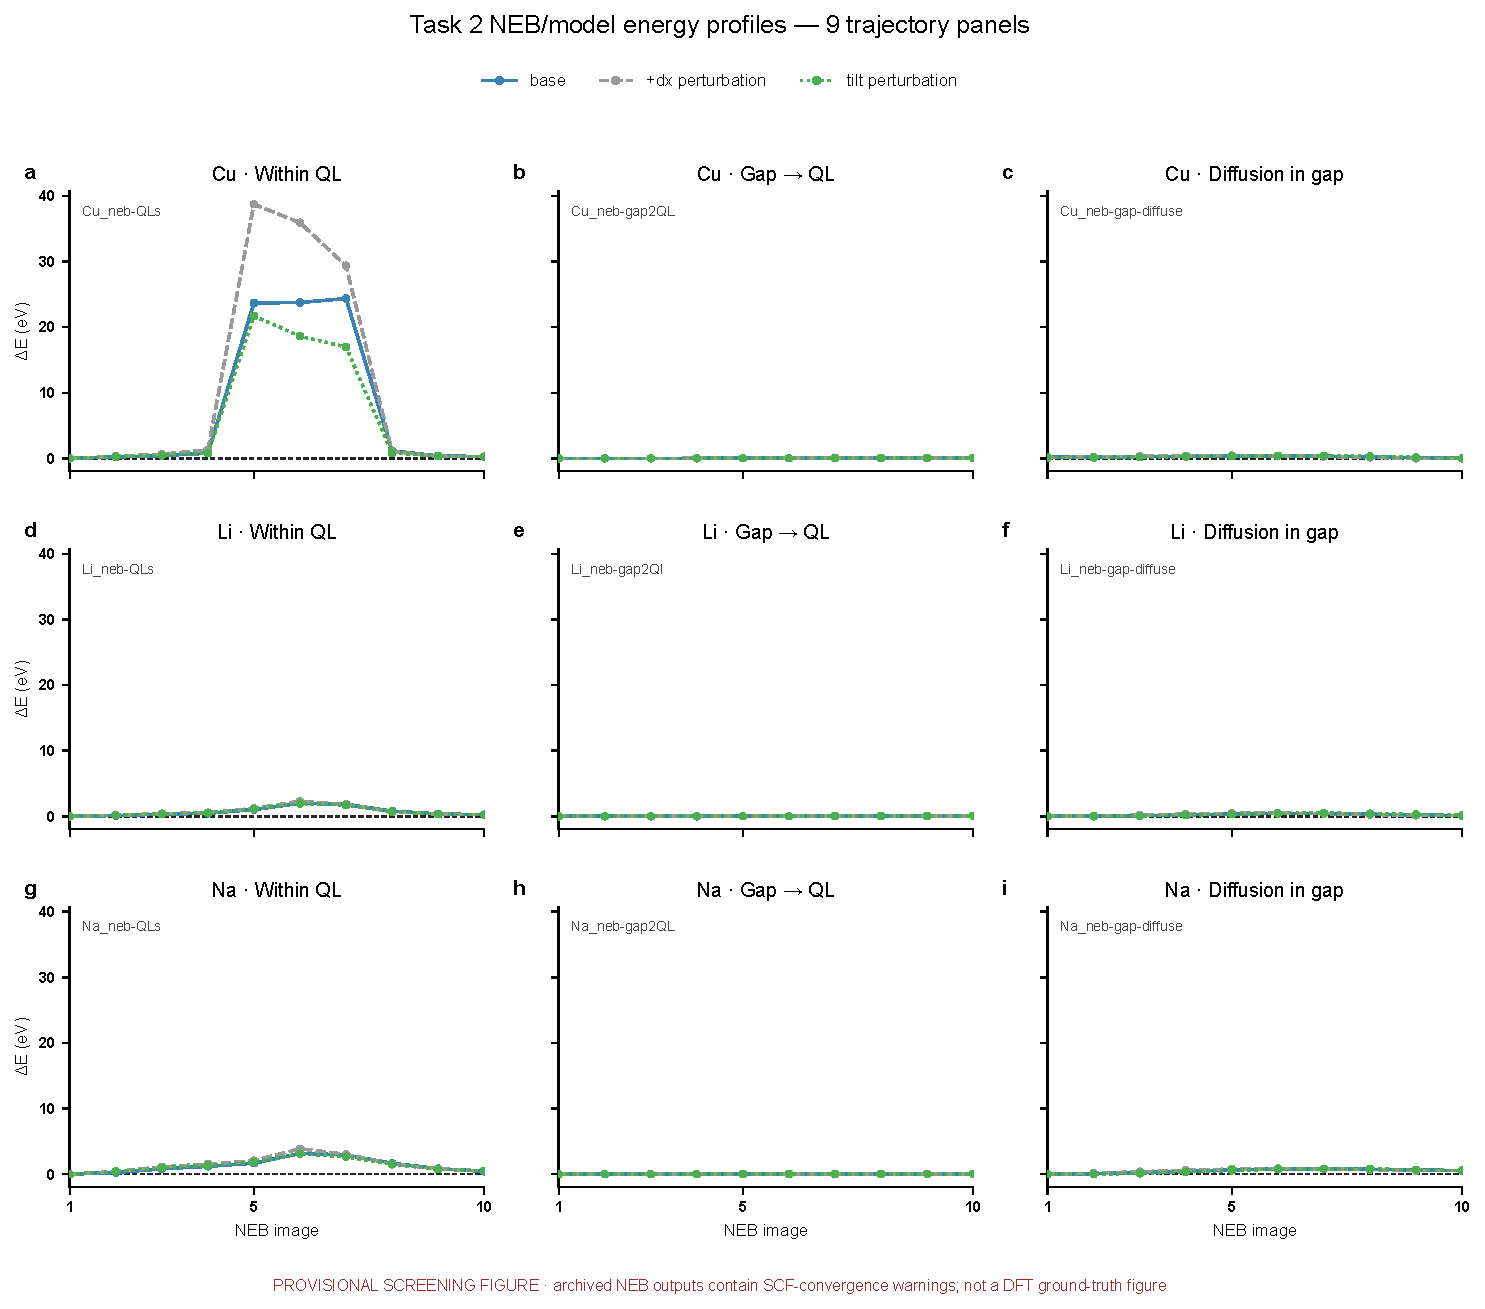
\includegraphics[width=\linewidth,height=0.42\textheight,keepaspectratio]{figure_pages/assets/fig_025.pdf}
\caption{Cross-element or multi-seed benchmark roster and pathway diagnostics. This page shows the candidate output ``Provisional task2 neb model profiles 9panel'' within the audited TASK2-ROSTER family. The panel identity, source scope, and current status are retained in the accompanying evidence matrix.}
\label{fig:candidate_025}
\end{figure}
\textbf{Results text draft.} The figure organizes the evaluated systems, seeds, models, or pathway families so that coverage and missing cells are visible. Provisional and audited rows are not pooled when their protocols or provenance differ.
\textbf{Discussion and boundary.} This is appropriate for SI coverage and provenance discussion. It should not be read as a single uncertainty distribution across model-level and path-level variation.
\textbf{Article placement.} Proposed article location: Results: cross-element transfer and seed stability.
\textbf{Reviewer linkage:} overall status PARTIAL.
\begin{itemize}[leftmargin=1.4em,noitemsep]
\item \textbf{REV-A1 (PARTIAL):} Reconcile Fig. 3d fixed-geometry DFT-path scoring with SI Fig. S3 self-consistent MLFF-NEB, including pathway identity and the DFT reference. \emph{Completed:} The fixed-path versus self-relaxed operator distinction and the narrower model-reported-barrier wording are integrated. \emph{Still required:} Close the restartable QE path-1--4 convergence gate, preserve the final path/source metadata, and complete the SI Fig. S3 endpoint/checkpoint/optimizer/source audit before calling the quantitative reference final.
\end{itemize}
\textbf{Evidence pointers.}
\begin{itemize}[leftmargin=1.4em,noitemsep]
\item Caption/text source: \begingroup\scriptsize\url{main/analysis/task2_cross_element/HEALTH_GATE_REPORT.md}\endgroup
\item Caption/text source: \begingroup\scriptsize\url{main/analysis/task2_cross_element/figures/provisional_task2_neb_model_profiles_9panel.metadata.txt}\endgroup
\end{itemize}
\statusline{\textbf{Audit gap / next action:} DFT gate is still open; do not write barrier-accuracy claims}
\vfill
\clearpage
\section{FIG-026 --- Placeholder dft gate status}
\label{figpage:fig-026}
\textbf{Group:} TASK2-ROSTER\quad \textbf{Evidence chain:} traceable\quad \textbf{Status:} placeholder
\begin{figure}[H]
\centering
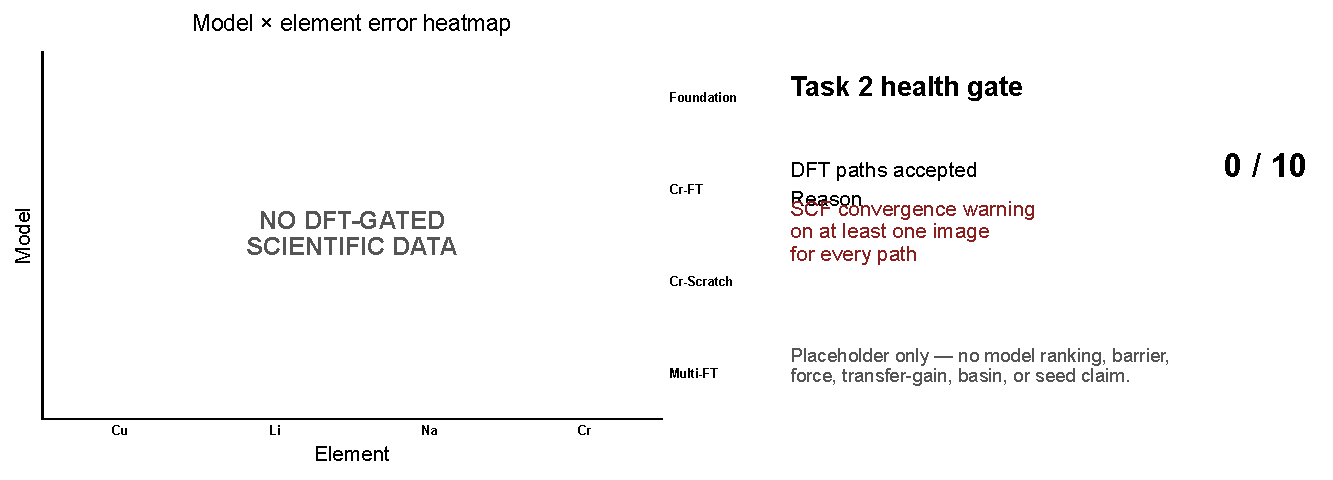
\includegraphics[width=\linewidth,height=0.42\textheight,keepaspectratio]{figure_pages/assets/fig_026.pdf}
\caption{Cross-element or multi-seed benchmark roster and pathway diagnostics. This page shows the candidate output ``Placeholder dft gate status'' within the audited TASK2-ROSTER family. The panel identity, source scope, and current status are retained in the accompanying evidence matrix.}
\label{fig:candidate_026}
\end{figure}
\textbf{Results text draft.} The figure organizes the evaluated systems, seeds, models, or pathway families so that coverage and missing cells are visible. Provisional and audited rows are not pooled when their protocols or provenance differ.
\textbf{Discussion and boundary.} This is appropriate for SI coverage and provenance discussion. It should not be read as a single uncertainty distribution across model-level and path-level variation.
\textbf{Article placement.} Proposed article location: Results: cross-element transfer and seed stability.
\textbf{Reviewer linkage:} overall status NO\_DIRECT\_REVIEWER\_FIGURE\_LINK.
No direct reviewer-response figure linkage was identified; this page is retained for scientific/article audit rather than as a direct reviewer response.
\textbf{Evidence pointers.}
\begin{itemize}[leftmargin=1.4em,noitemsep]
\item Caption/text source: \begingroup\scriptsize\url{main/analysis/task2_cross_element_broad_roster_20261003/HEALTH_GATE_REPORT.md}\endgroup
\end{itemize}
\statusline{\textbf{Audit gap / next action:} DFT gate is still open; do not write barrier-accuracy claims}
\vfill
\clearpage
\section{FIG-027 --- Task2 broad roster diagnostic}
\label{figpage:fig-027}
\textbf{Group:} TASK2-ROSTER\quad \textbf{Evidence chain:} traceable\quad \textbf{Status:} exploratory
\begin{figure}[H]
\centering
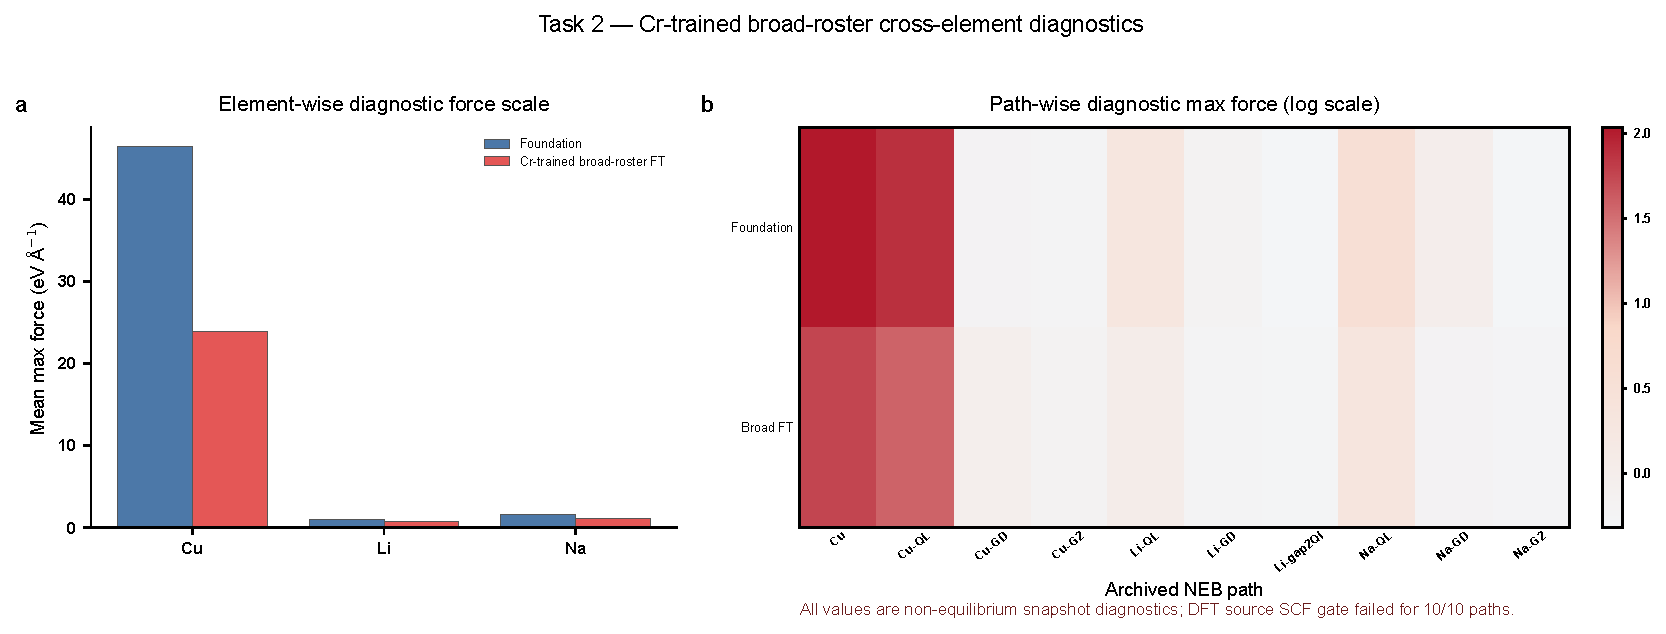
\includegraphics[width=\linewidth,height=0.42\textheight,keepaspectratio]{figure_pages/assets/fig_027.pdf}
\caption{Cross-element or multi-seed benchmark roster and pathway diagnostics. This page shows the candidate output ``Task2 broad roster diagnostic'' within the audited TASK2-ROSTER family. The panel identity, source scope, and current status are retained in the accompanying evidence matrix.}
\label{fig:candidate_027}
\end{figure}
\textbf{Results text draft.} The figure organizes the evaluated systems, seeds, models, or pathway families so that coverage and missing cells are visible. Provisional and audited rows are not pooled when their protocols or provenance differ.
\textbf{Discussion and boundary.} This is appropriate for SI coverage and provenance discussion. It should not be read as a single uncertainty distribution across model-level and path-level variation.
\textbf{Article placement.} Proposed article location: Results: cross-element transfer and seed stability.
\textbf{Reviewer linkage:} overall status NO\_DIRECT\_REVIEWER\_FIGURE\_LINK.
No direct reviewer-response figure linkage was identified; this page is retained for scientific/article audit rather than as a direct reviewer response.
\textbf{Evidence pointers.}
\begin{itemize}[leftmargin=1.4em,noitemsep]
\item Caption/text source: \begingroup\scriptsize\url{main/analysis/task2_cross_element_broad_roster_20261003/HEALTH_GATE_REPORT.md}\endgroup
\end{itemize}
\statusline{\textbf{Audit gap / next action:} DFT gate is still open; do not write barrier-accuracy claims}
\vfill
\clearpage
\section{FIG-028 --- Task2 broad roster profiles}
\label{figpage:fig-028}
\textbf{Group:} TASK2-ROSTER\quad \textbf{Evidence chain:} traceable\quad \textbf{Status:} comparison
\begin{figure}[H]
\centering
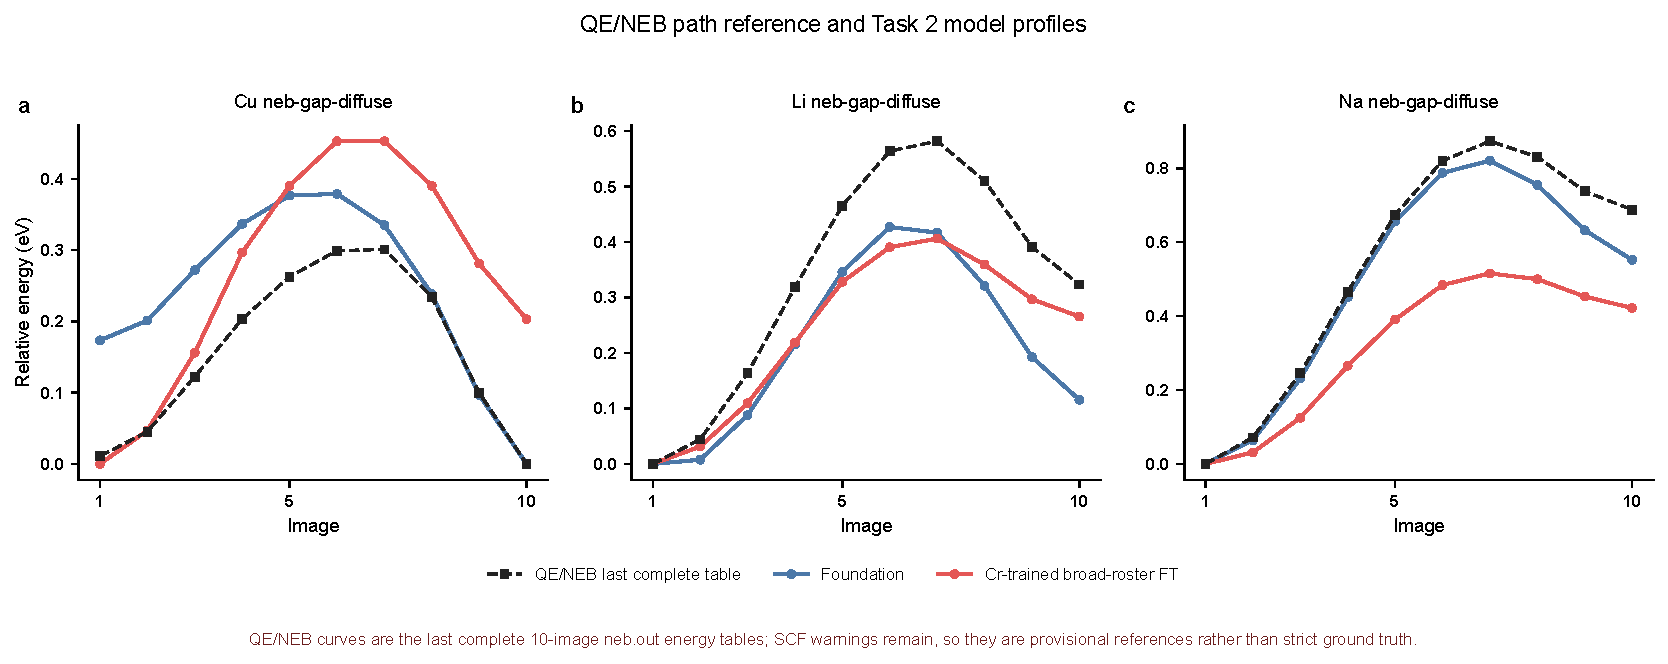
\includegraphics[width=\linewidth,height=0.42\textheight,keepaspectratio]{figure_pages/assets/fig_028.pdf}
\caption{Cross-element or multi-seed benchmark roster and pathway diagnostics. This page shows the candidate output ``Task2 broad roster profiles'' within the audited TASK2-ROSTER family. The panel identity, source scope, and current status are retained in the accompanying evidence matrix.}
\label{fig:candidate_028}
\end{figure}
\textbf{Results text draft.} The figure organizes the evaluated systems, seeds, models, or pathway families so that coverage and missing cells are visible. Provisional and audited rows are not pooled when their protocols or provenance differ.
\textbf{Discussion and boundary.} This is appropriate for SI coverage and provenance discussion. It should not be read as a single uncertainty distribution across model-level and path-level variation.
\textbf{Article placement.} Proposed article location: Results: cross-element transfer and seed stability.
\textbf{Reviewer linkage:} overall status NO\_DIRECT\_REVIEWER\_FIGURE\_LINK.
No direct reviewer-response figure linkage was identified; this page is retained for scientific/article audit rather than as a direct reviewer response.
\textbf{Evidence pointers.}
\begin{itemize}[leftmargin=1.4em,noitemsep]
\item Caption/text source: \begingroup\scriptsize\url{main/analysis/task2_cross_element_broad_roster_20261003/HEALTH_GATE_REPORT.md}\endgroup
\end{itemize}
\statusline{\textbf{Audit gap / next action:} DFT gate is still open; do not write barrier-accuracy claims}
\vfill
\clearpage
\section{FIG-029 --- Task2 broad roster profiles 9panel}
\label{figpage:fig-029}
\textbf{Group:} TASK2-ROSTER\quad \textbf{Evidence chain:} traceable\quad \textbf{Status:} comparison
\begin{figure}[H]
\centering
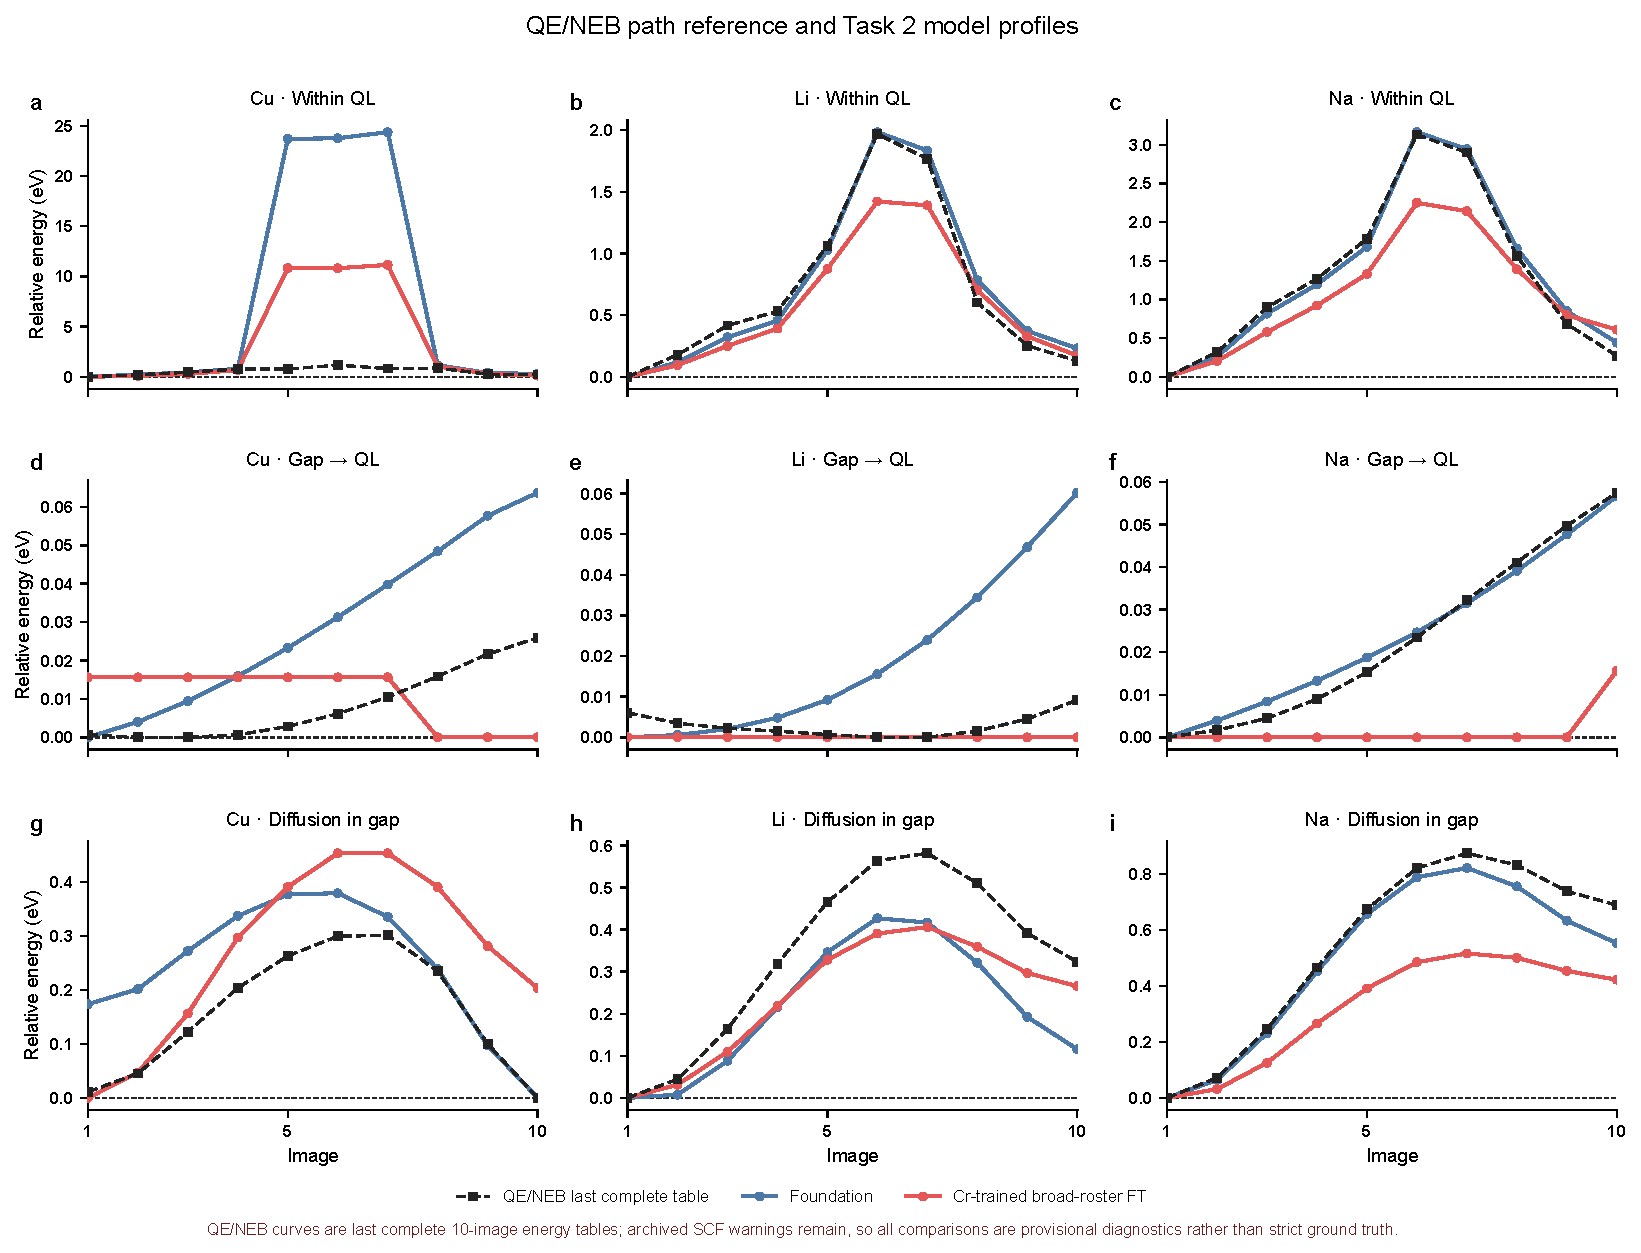
\includegraphics[width=\linewidth,height=0.42\textheight,keepaspectratio]{figure_pages/assets/fig_029.pdf}
\caption{Cross-element or multi-seed benchmark roster and pathway diagnostics. This page shows the candidate output ``Task2 broad roster profiles 9panel'' within the audited TASK2-ROSTER family. The panel identity, source scope, and current status are retained in the accompanying evidence matrix.}
\label{fig:candidate_029}
\end{figure}
\textbf{Results text draft.} The figure organizes the evaluated systems, seeds, models, or pathway families so that coverage and missing cells are visible. Provisional and audited rows are not pooled when their protocols or provenance differ.
\textbf{Discussion and boundary.} This is appropriate for SI coverage and provenance discussion. It should not be read as a single uncertainty distribution across model-level and path-level variation.
\textbf{Article placement.} Proposed article location: Results: cross-element transfer and seed stability.
\textbf{Reviewer linkage:} overall status NO\_DIRECT\_REVIEWER\_FIGURE\_LINK.
No direct reviewer-response figure linkage was identified; this page is retained for scientific/article audit rather than as a direct reviewer response.
\textbf{Evidence pointers.}
\begin{itemize}[leftmargin=1.4em,noitemsep]
\item Caption/text source: \begingroup\scriptsize\url{main/analysis/task2_cross_element_broad_roster_20261003/HEALTH_GATE_REPORT.md}\endgroup
\end{itemize}
\statusline{\textbf{Audit gap / next action:} DFT gate is still open; do not write barrier-accuracy claims}
\vfill
\clearpage
\section{FIG-030 --- Task2 three seed profiles}
\label{figpage:fig-030}
\textbf{Group:} TASK2-ROSTER\quad \textbf{Evidence chain:} traceable\quad \textbf{Status:} publication;comparison
\begin{figure}[H]
\centering
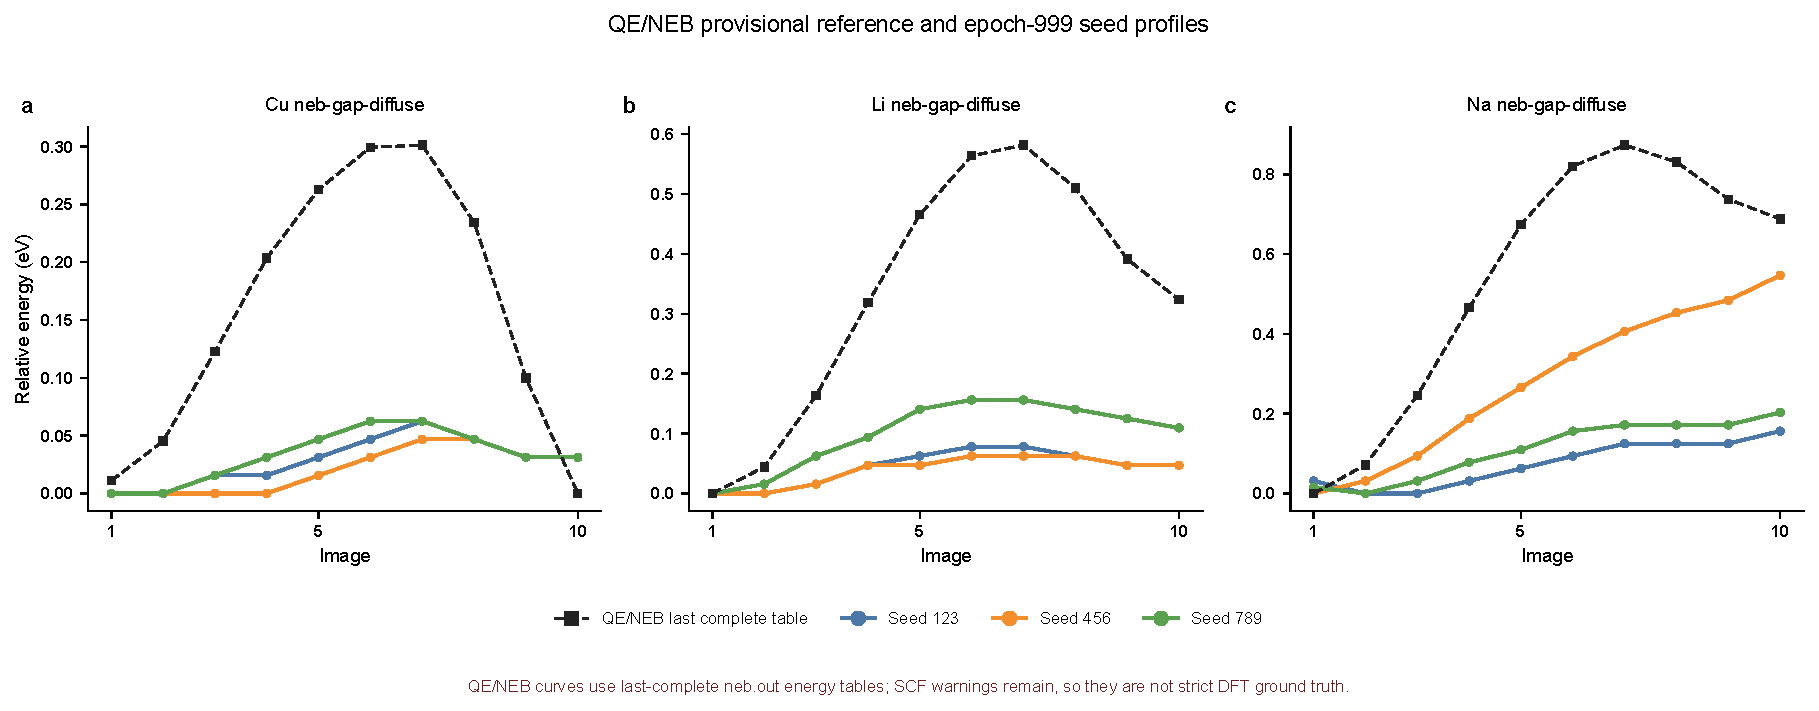
\includegraphics[width=\linewidth,height=0.42\textheight,keepaspectratio]{figure_pages/assets/fig_030.pdf}
\caption{Cross-element or multi-seed benchmark roster and pathway diagnostics. This page shows the candidate output ``Task2 three seed profiles'' within the audited TASK2-ROSTER family. The panel identity, source scope, and current status are retained in the accompanying evidence matrix.}
\label{fig:candidate_030}
\end{figure}
\textbf{Results text draft.} The figure organizes the evaluated systems, seeds, models, or pathway families so that coverage and missing cells are visible. Provisional and audited rows are not pooled when their protocols or provenance differ.
\textbf{Discussion and boundary.} This is appropriate for SI coverage and provenance discussion. It should not be read as a single uncertainty distribution across model-level and path-level variation.
\textbf{Article placement.} Proposed article location: Results: cross-element transfer and seed stability.
\textbf{Reviewer linkage:} overall status NO\_DIRECT\_REVIEWER\_FIGURE\_LINK.
No direct reviewer-response figure linkage was identified; this page is retained for scientific/article audit rather than as a direct reviewer response.
\textbf{Evidence pointers.}
\begin{itemize}[leftmargin=1.4em,noitemsep]
\item Caption/text source: \begingroup\scriptsize\url{main/analysis/task2_cross_element_broad_roster_final_20261006/HEALTH_GATE_REPORT.md}\endgroup
\item Caption/text source: \begingroup\scriptsize\url{main/analysis/task2_cross_element_broad_roster_final_20261006/README.md}\endgroup
\end{itemize}
\statusline{\textbf{Audit gap / next action:} DFT gate is still open; do not write barrier-accuracy claims}
\vfill
\clearpage
\section{FIG-031 --- Task2 three seed stability}
\label{figpage:fig-031}
\textbf{Group:} TASK2-ROSTER\quad \textbf{Evidence chain:} traceable\quad \textbf{Status:} publication
\begin{figure}[H]
\centering
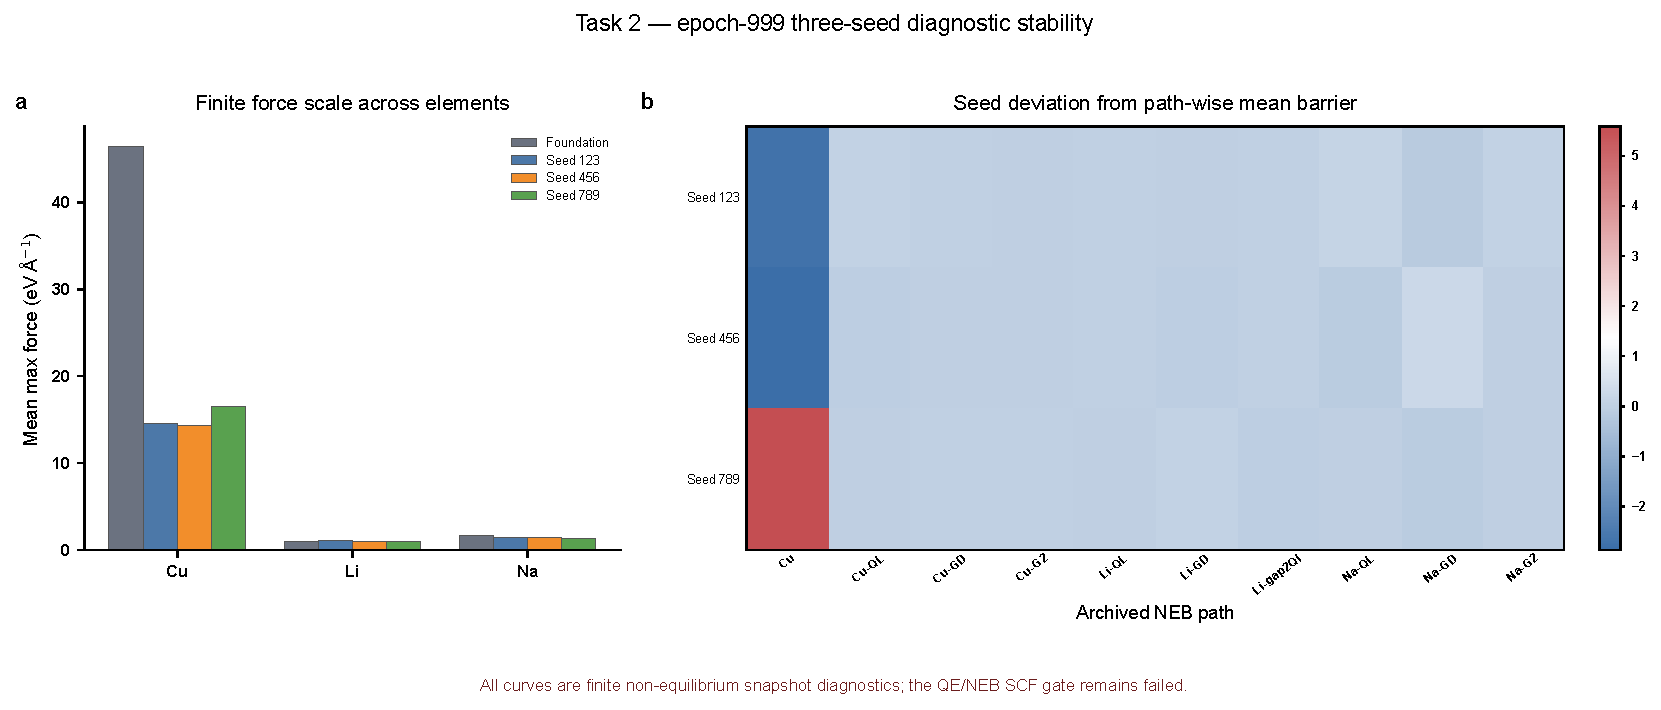
\includegraphics[width=\linewidth,height=0.42\textheight,keepaspectratio]{figure_pages/assets/fig_031.pdf}
\caption{Cross-element or multi-seed benchmark roster and pathway diagnostics. This page shows the candidate output ``Task2 three seed stability'' within the audited TASK2-ROSTER family. The panel identity, source scope, and current status are retained in the accompanying evidence matrix.}
\label{fig:candidate_031}
\end{figure}
\textbf{Results text draft.} The figure organizes the evaluated systems, seeds, models, or pathway families so that coverage and missing cells are visible. Provisional and audited rows are not pooled when their protocols or provenance differ.
\textbf{Discussion and boundary.} This is appropriate for SI coverage and provenance discussion. It should not be read as a single uncertainty distribution across model-level and path-level variation.
\textbf{Article placement.} Proposed article location: Results: cross-element transfer and seed stability.
\textbf{Reviewer linkage:} overall status NO\_DIRECT\_REVIEWER\_FIGURE\_LINK.
No direct reviewer-response figure linkage was identified; this page is retained for scientific/article audit rather than as a direct reviewer response.
\textbf{Evidence pointers.}
\begin{itemize}[leftmargin=1.4em,noitemsep]
\item Caption/text source: \begingroup\scriptsize\url{main/analysis/task2_cross_element_broad_roster_final_20261006/HEALTH_GATE_REPORT.md}\endgroup
\item Caption/text source: \begingroup\scriptsize\url{main/analysis/task2_cross_element_broad_roster_final_20261006/README.md}\endgroup
\end{itemize}
\statusline{\textbf{Audit gap / next action:} DFT gate is still open; do not write barrier-accuracy claims}
\vfill
\clearpage
\section{FIG-032 --- Task2 three seed validation}
\label{figpage:fig-032}
\textbf{Group:} TASK2-ROSTER\quad \textbf{Evidence chain:} traceable\quad \textbf{Status:} publication
\begin{figure}[H]
\centering
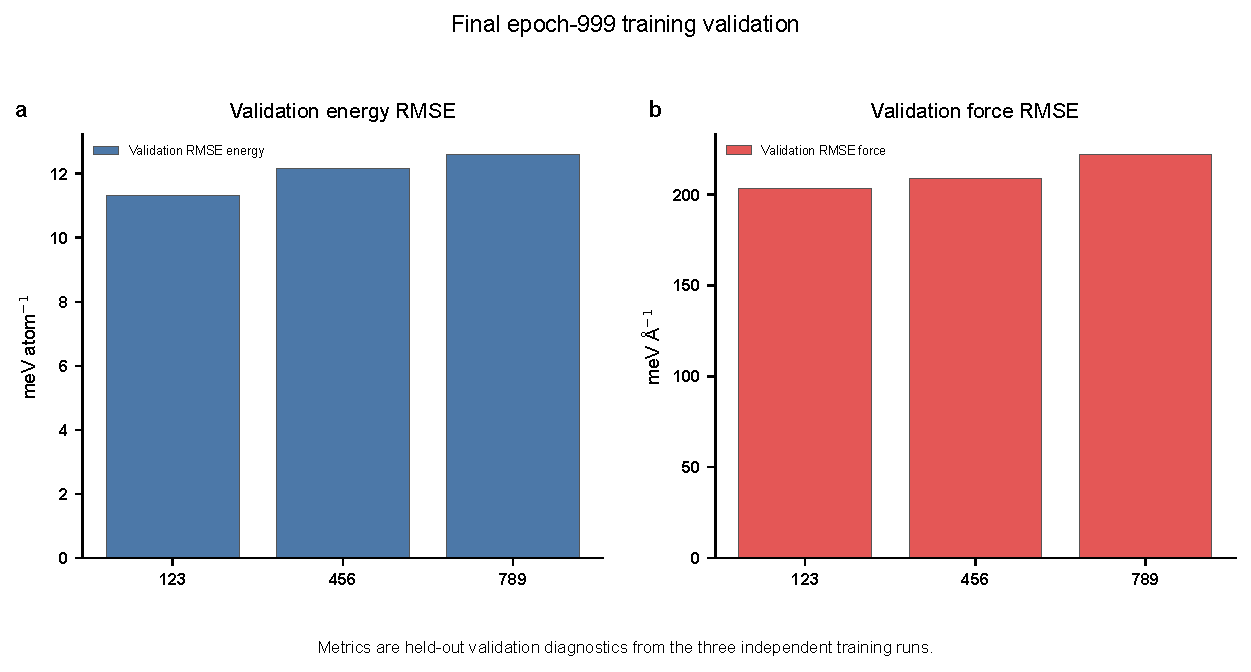
\includegraphics[width=\linewidth,height=0.42\textheight,keepaspectratio]{figure_pages/assets/fig_032.pdf}
\caption{Cross-element or multi-seed benchmark roster and pathway diagnostics. This page shows the candidate output ``Task2 three seed validation'' within the audited TASK2-ROSTER family. The panel identity, source scope, and current status are retained in the accompanying evidence matrix.}
\label{fig:candidate_032}
\end{figure}
\textbf{Results text draft.} The figure organizes the evaluated systems, seeds, models, or pathway families so that coverage and missing cells are visible. Provisional and audited rows are not pooled when their protocols or provenance differ.
\textbf{Discussion and boundary.} This is appropriate for SI coverage and provenance discussion. It should not be read as a single uncertainty distribution across model-level and path-level variation.
\textbf{Article placement.} Proposed article location: Results: cross-element transfer and seed stability.
\textbf{Reviewer linkage:} overall status NO\_DIRECT\_REVIEWER\_FIGURE\_LINK.
No direct reviewer-response figure linkage was identified; this page is retained for scientific/article audit rather than as a direct reviewer response.
\textbf{Evidence pointers.}
\begin{itemize}[leftmargin=1.4em,noitemsep]
\item Caption/text source: \begingroup\scriptsize\url{main/analysis/task2_cross_element_broad_roster_final_20261006/HEALTH_GATE_REPORT.md}\endgroup
\item Caption/text source: \begingroup\scriptsize\url{main/analysis/task2_cross_element_broad_roster_final_20261006/README.md}\endgroup
\end{itemize}
\statusline{\textbf{Audit gap / next action:} DFT gate is still open; do not write barrier-accuracy claims}
\vfill
\clearpage
\section{FIG-033 --- Endpoint initialization smoke}
\label{figpage:fig-033}
\textbf{Group:} TASK3-NEB\quad \textbf{Evidence chain:} partial\quad \textbf{Status:} unclassified
\begin{figure}[H]
\centering
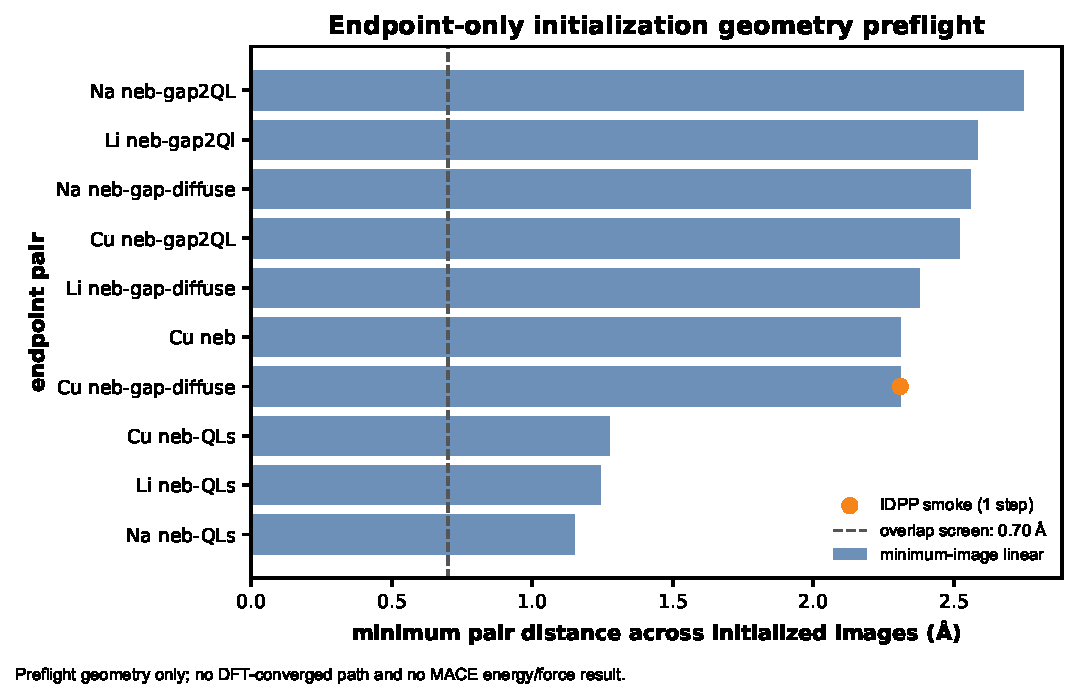
\includegraphics[width=\linewidth,height=0.42\textheight,keepaspectratio]{figure_pages/assets/fig_033.pdf}
\caption{Neb pathway, barrier, topology, or self-consistency diagnostics. This page shows the candidate output ``Endpoint initialization smoke'' within the audited TASK3-NEB family. The panel identity, source scope, and current status are retained in the accompanying evidence matrix.}
\label{fig:candidate_033}
\end{figure}
\textbf{Results text draft.} The panels distinguish fixed-path scoring, self-consistent MLFF-NEB behavior, endpoint/path topology checks, and DFT convergence status. These operators answer different questions and are kept separate in the text.
\textbf{Discussion and boundary.} A model-reported self-relaxed barrier must not be presented as the fixed-path DFT error, and a provisional or unconverged DFT path must not be promoted to a final reference barrier.
\textbf{Article placement.} Proposed article location: Results or SI: path-family diagnostics.
\textbf{Reviewer linkage:} overall status PARTIAL.
\begin{itemize}[leftmargin=1.4em,noitemsep]
\item \textbf{REV-A1 (PARTIAL):} Reconcile Fig. 3d fixed-geometry DFT-path scoring with SI Fig. S3 self-consistent MLFF-NEB, including pathway identity and the DFT reference. \emph{Completed:} The fixed-path versus self-relaxed operator distinction and the narrower model-reported-barrier wording are integrated. \emph{Still required:} Close the restartable QE path-1--4 convergence gate, preserve the final path/source metadata, and complete the SI Fig. S3 endpoint/checkpoint/optimizer/source audit before calling the quantitative reference final.
\end{itemize}
\textbf{Evidence pointers.}
\begin{itemize}[leftmargin=1.4em,noitemsep]
\item Data/processed: \begingroup\scriptsize\url{main/analysis/task3_endpoint_only_neb/dft_gate_manifest.csv}\endgroup
\item Data/processed: \begingroup\scriptsize\url{main/analysis/task3_endpoint_only_neb/endpoint_only_leakage_audit.csv}\endgroup
\item Plot/processing script: \begingroup\scriptsize\url{main/analysis/task3_endpoint_only_neb/analyze_all_foundation_models.py}\endgroup
\item Plot/processing script: \begingroup\scriptsize\url{main/analysis/task3_endpoint_only_neb/analyze_corrected_dft_foundation_comparison.py}\endgroup
\item Caption/text source: \begingroup\scriptsize\url{main/analysis/task3_endpoint_only_neb/README.md}\endgroup
\end{itemize}
\statusline{\textbf{Audit gap / next action:} Many per-path exports have no co-located generator; use the parent renderer and record the exact input tables}
\vfill
\clearpage
\section{FIG-034 --- Figure corrected dft foundation barrier comparison}
\label{figpage:fig-034}
\textbf{Group:} TASK3-NEB\quad \textbf{Evidence chain:} partial\quad \textbf{Status:} exploratory;audit;comparison
\begin{figure}[H]
\centering
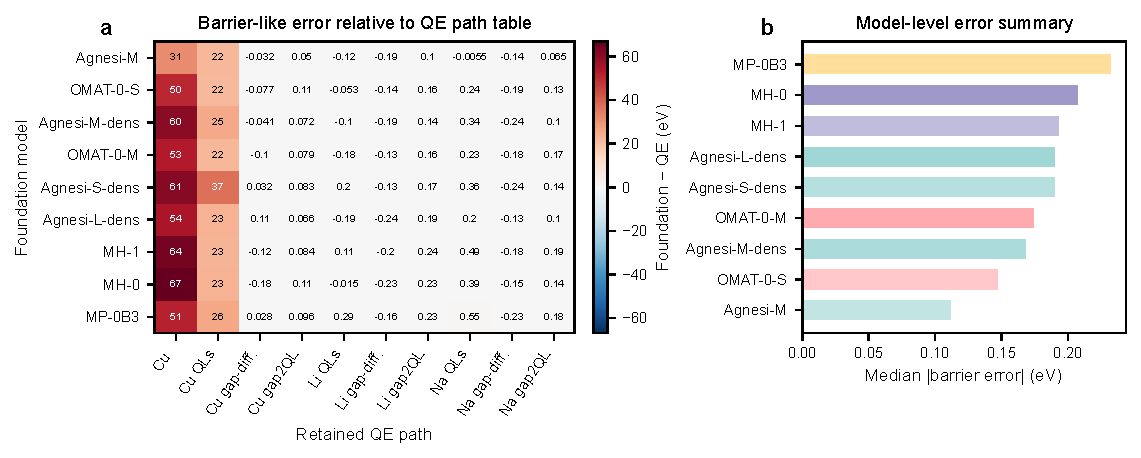
\includegraphics[width=\linewidth,height=0.42\textheight,keepaspectratio]{figure_pages/assets/fig_034.pdf}
\caption{Neb pathway, barrier, topology, or self-consistency diagnostics. This page shows the candidate output ``Figure corrected dft foundation barrier comparison'' within the audited TASK3-NEB family. The panel identity, source scope, and current status are retained in the accompanying evidence matrix.}
\label{fig:candidate_034}
\end{figure}
\textbf{Results text draft.} The panels distinguish fixed-path scoring, self-consistent MLFF-NEB behavior, endpoint/path topology checks, and DFT convergence status. These operators answer different questions and are kept separate in the text.
\textbf{Discussion and boundary.} A model-reported self-relaxed barrier must not be presented as the fixed-path DFT error, and a provisional or unconverged DFT path must not be promoted to a final reference barrier.
\textbf{Article placement.} Proposed article location: Results or SI: path-family diagnostics.
\textbf{Reviewer linkage:} overall status PARTIAL.
\begin{itemize}[leftmargin=1.4em,noitemsep]
\item \textbf{REV-A1 (PARTIAL):} Reconcile Fig. 3d fixed-geometry DFT-path scoring with SI Fig. S3 self-consistent MLFF-NEB, including pathway identity and the DFT reference. \emph{Completed:} The fixed-path versus self-relaxed operator distinction and the narrower model-reported-barrier wording are integrated. \emph{Still required:} Close the restartable QE path-1--4 convergence gate, preserve the final path/source metadata, and complete the SI Fig. S3 endpoint/checkpoint/optimizer/source audit before calling the quantitative reference final.
\end{itemize}
\textbf{Evidence pointers.}
\begin{itemize}[leftmargin=1.4em,noitemsep]
\item Data/processed: \begingroup\scriptsize\url{main/analysis/task3_endpoint_only_neb/exploratory_energy_audit/all_dft_foundation_models/corrected_dft_foundation_image_profiles.csv}\endgroup
\item Data/processed: \begingroup\scriptsize\url{main/analysis/task3_endpoint_only_neb/exploratory_energy_audit/all_dft_foundation_models/corrected_dft_foundation_manifest.json}\endgroup
\item Plot/processing script: \begingroup\scriptsize\url{main/analysis/task3_endpoint_only_neb/exploratory_energy_audit/plot_paper_figures.py}\endgroup
\item Caption/text source: \begingroup\scriptsize\url{main/analysis/task3_endpoint_only_neb/exploratory_energy_audit/ACCEPTANCE_MATRIX.md}\endgroup
\item Caption/text source: \begingroup\scriptsize\url{main/analysis/task3_endpoint_only_neb/exploratory_energy_audit/EXPLORATORY_REPORT.md}\endgroup
\end{itemize}
\statusline{\textbf{Audit gap / next action:} Many per-path exports have no co-located generator; use the parent renderer and record the exact input tables}
\vfill
\clearpage
\section{FIG-035 --- Figure corrected dft foundation path profiles}
\label{figpage:fig-035}
\textbf{Group:} TASK3-NEB\quad \textbf{Evidence chain:} partial\quad \textbf{Status:} exploratory;audit;comparison
\begin{figure}[H]
\centering
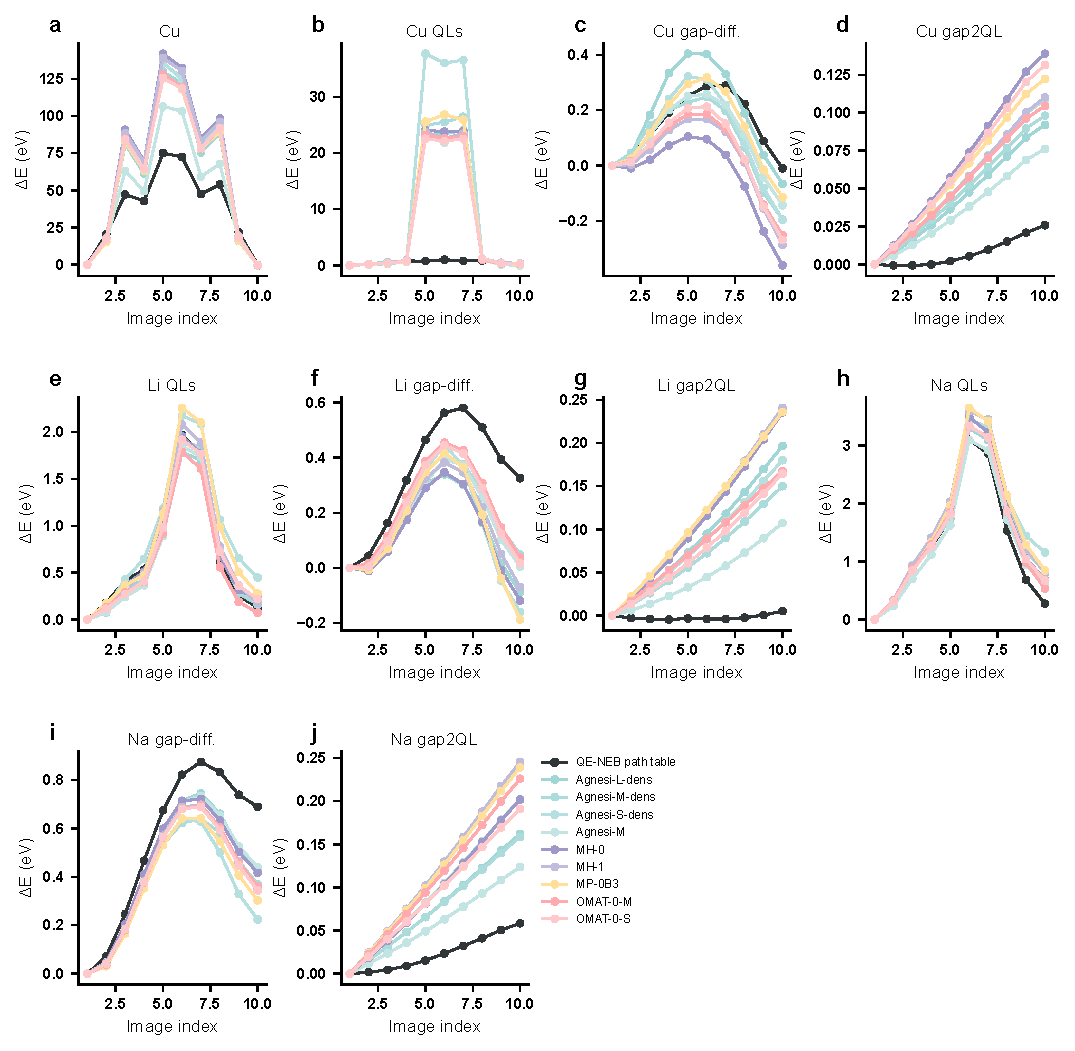
\includegraphics[width=\linewidth,height=0.42\textheight,keepaspectratio]{figure_pages/assets/fig_035.pdf}
\caption{Neb pathway, barrier, topology, or self-consistency diagnostics. This page shows the candidate output ``Figure corrected dft foundation path profiles'' within the audited TASK3-NEB family. The panel identity, source scope, and current status are retained in the accompanying evidence matrix.}
\label{fig:candidate_035}
\end{figure}
\textbf{Results text draft.} The panels distinguish fixed-path scoring, self-consistent MLFF-NEB behavior, endpoint/path topology checks, and DFT convergence status. These operators answer different questions and are kept separate in the text.
\textbf{Discussion and boundary.} A model-reported self-relaxed barrier must not be presented as the fixed-path DFT error, and a provisional or unconverged DFT path must not be promoted to a final reference barrier.
\textbf{Article placement.} Proposed article location: Results or SI: path-family diagnostics.
\textbf{Reviewer linkage:} overall status PARTIAL.
\begin{itemize}[leftmargin=1.4em,noitemsep]
\item \textbf{REV-A1 (PARTIAL):} Reconcile Fig. 3d fixed-geometry DFT-path scoring with SI Fig. S3 self-consistent MLFF-NEB, including pathway identity and the DFT reference. \emph{Completed:} The fixed-path versus self-relaxed operator distinction and the narrower model-reported-barrier wording are integrated. \emph{Still required:} Close the restartable QE path-1--4 convergence gate, preserve the final path/source metadata, and complete the SI Fig. S3 endpoint/checkpoint/optimizer/source audit before calling the quantitative reference final.
\end{itemize}
\textbf{Evidence pointers.}
\begin{itemize}[leftmargin=1.4em,noitemsep]
\item Data/processed: \begingroup\scriptsize\url{main/analysis/task3_endpoint_only_neb/exploratory_energy_audit/all_dft_foundation_models/corrected_dft_foundation_image_profiles.csv}\endgroup
\item Data/processed: \begingroup\scriptsize\url{main/analysis/task3_endpoint_only_neb/exploratory_energy_audit/all_dft_foundation_models/corrected_dft_foundation_manifest.json}\endgroup
\item Plot/processing script: \begingroup\scriptsize\url{main/analysis/task3_endpoint_only_neb/exploratory_energy_audit/plot_paper_figures.py}\endgroup
\item Caption/text source: \begingroup\scriptsize\url{main/analysis/task3_endpoint_only_neb/exploratory_energy_audit/ACCEPTANCE_MATRIX.md}\endgroup
\item Caption/text source: \begingroup\scriptsize\url{main/analysis/task3_endpoint_only_neb/exploratory_energy_audit/EXPLORATORY_REPORT.md}\endgroup
\end{itemize}
\statusline{\textbf{Audit gap / next action:} Many per-path exports have no co-located generator; use the parent renderer and record the exact input tables}
\vfill
\clearpage
\section{FIG-036 --- Figure diagnostic framework overview}
\label{figpage:fig-036}
\textbf{Group:} TASK3-NEB\quad \textbf{Evidence chain:} partial\quad \textbf{Status:} exploratory;audit
\begin{figure}[H]
\centering
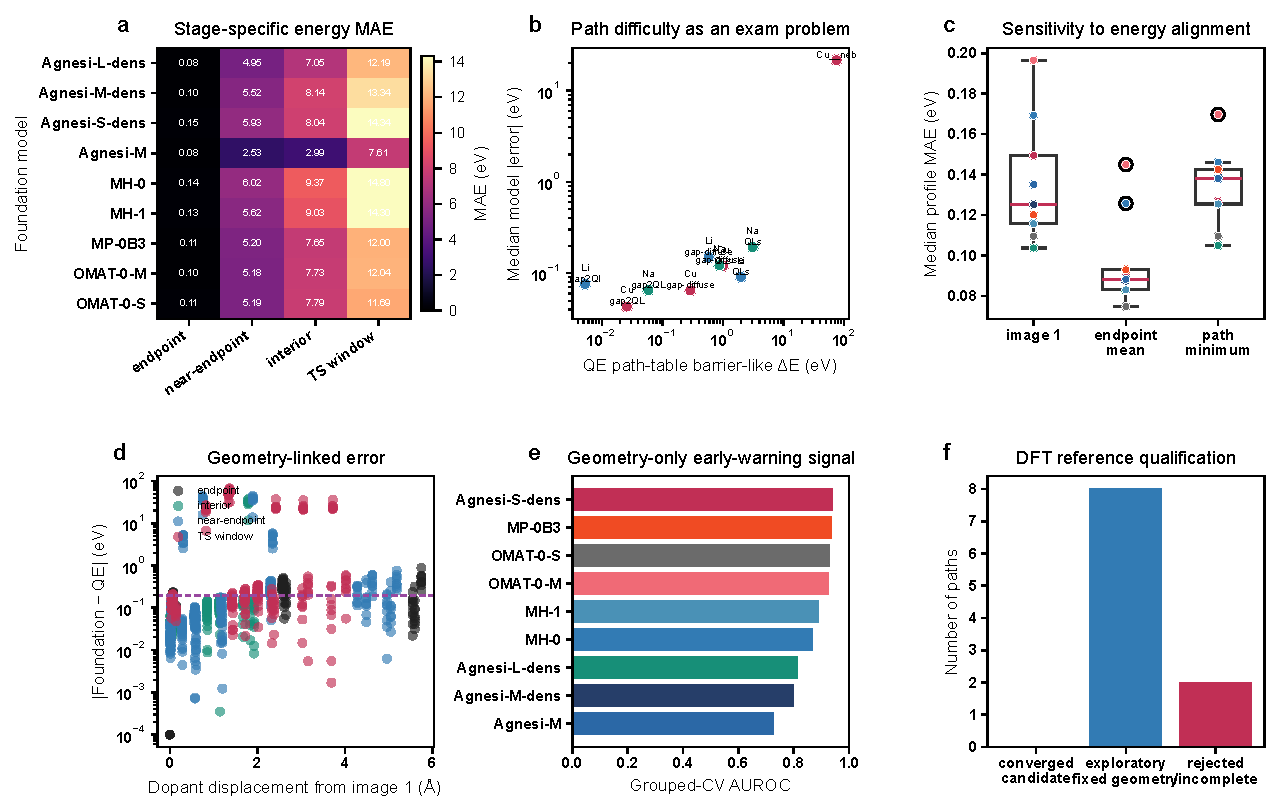
\includegraphics[width=\linewidth,height=0.42\textheight,keepaspectratio]{figure_pages/assets/fig_036.pdf}
\caption{Neb pathway, barrier, topology, or self-consistency diagnostics. This page shows the candidate output ``Figure diagnostic framework overview'' within the audited TASK3-NEB family. The panel identity, source scope, and current status are retained in the accompanying evidence matrix.}
\label{fig:candidate_036}
\end{figure}
\textbf{Results text draft.} The panels distinguish fixed-path scoring, self-consistent MLFF-NEB behavior, endpoint/path topology checks, and DFT convergence status. These operators answer different questions and are kept separate in the text.
\textbf{Discussion and boundary.} A model-reported self-relaxed barrier must not be presented as the fixed-path DFT error, and a provisional or unconverged DFT path must not be promoted to a final reference barrier.
\textbf{Article placement.} Proposed article location: Results or SI: path-family diagnostics.
\textbf{Reviewer linkage:} overall status PARTIAL.
\begin{itemize}[leftmargin=1.4em,noitemsep]
\item \textbf{REV-A1 (PARTIAL):} Reconcile Fig. 3d fixed-geometry DFT-path scoring with SI Fig. S3 self-consistent MLFF-NEB, including pathway identity and the DFT reference. \emph{Completed:} The fixed-path versus self-relaxed operator distinction and the narrower model-reported-barrier wording are integrated. \emph{Still required:} Close the restartable QE path-1--4 convergence gate, preserve the final path/source metadata, and complete the SI Fig. S3 endpoint/checkpoint/optimizer/source audit before calling the quantitative reference final.
\end{itemize}
\textbf{Evidence pointers.}
\begin{itemize}[leftmargin=1.4em,noitemsep]
\item Data/processed: \begingroup\scriptsize\url{main/analysis/task3_endpoint_only_neb/exploratory_energy_audit/all_path_diagnostic_framework/alignment_profile_errors.csv}\endgroup
\item Data/processed: \begingroup\scriptsize\url{main/analysis/task3_endpoint_only_neb/exploratory_energy_audit/all_path_diagnostic_framework/alignment_sensitivity_summary.csv}\endgroup
\item Plot/processing script: \begingroup\scriptsize\url{main/analysis/task3_endpoint_only_neb/exploratory_energy_audit/plot_paper_figures.py}\endgroup
\item Caption/text source: \begingroup\scriptsize\url{main/analysis/task3_endpoint_only_neb/exploratory_energy_audit/ACCEPTANCE_MATRIX.md}\endgroup
\item Caption/text source: \begingroup\scriptsize\url{main/analysis/task3_endpoint_only_neb/exploratory_energy_audit/EXPLORATORY_REPORT.md}\endgroup
\end{itemize}
\statusline{\textbf{Audit gap / next action:} Many per-path exports have no co-located generator; use the parent renderer and record the exact input tables}
\vfill
\clearpage
\section{FIG-037 --- Figure path type summary}
\label{figpage:fig-037}
\textbf{Group:} TASK3-NEB\quad \textbf{Evidence chain:} partial\quad \textbf{Status:} exploratory;audit
\begin{figure}[H]
\centering
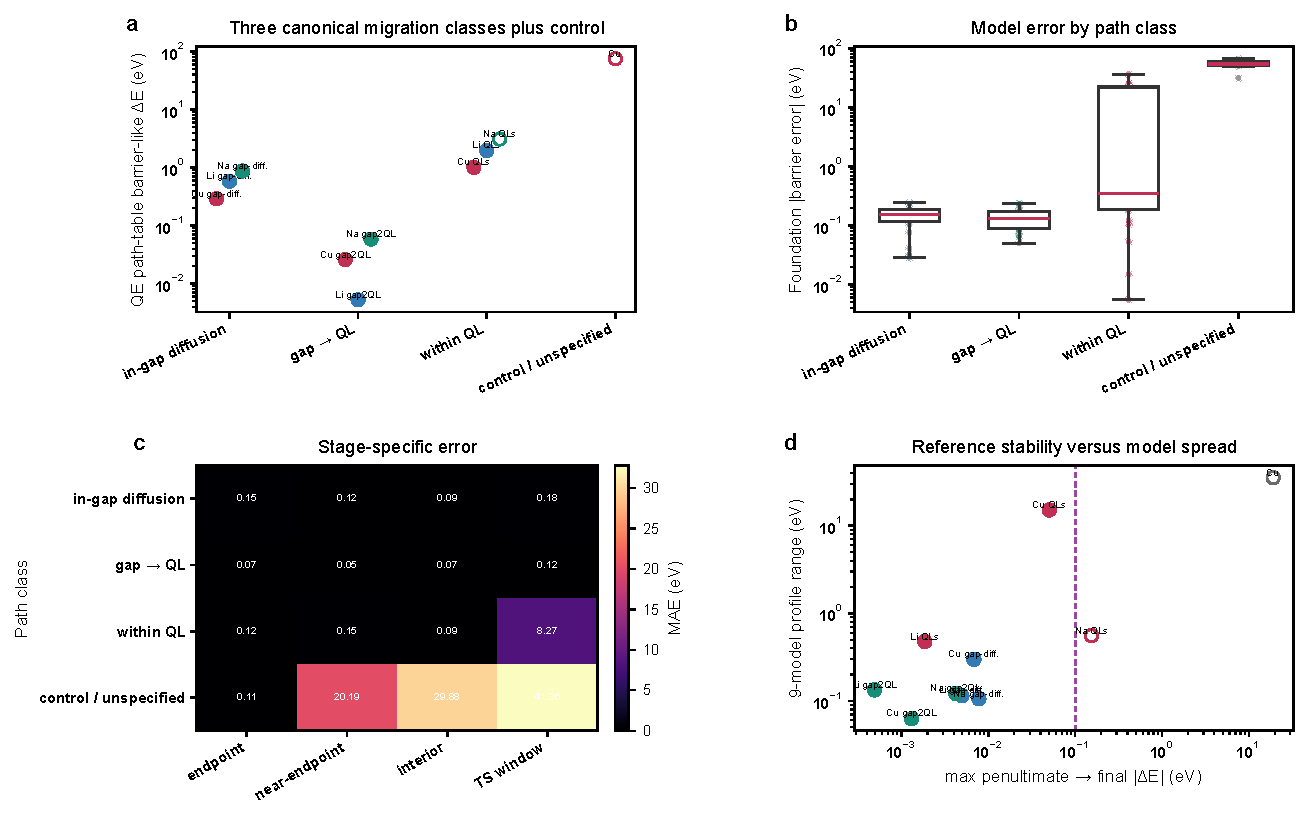
\includegraphics[width=\linewidth,height=0.42\textheight,keepaspectratio]{figure_pages/assets/fig_037.pdf}
\caption{Neb pathway, barrier, topology, or self-consistency diagnostics. This page shows the candidate output ``Figure path type summary'' within the audited TASK3-NEB family. The panel identity, source scope, and current status are retained in the accompanying evidence matrix.}
\label{fig:candidate_037}
\end{figure}
\textbf{Results text draft.} The panels distinguish fixed-path scoring, self-consistent MLFF-NEB behavior, endpoint/path topology checks, and DFT convergence status. These operators answer different questions and are kept separate in the text.
\textbf{Discussion and boundary.} A model-reported self-relaxed barrier must not be presented as the fixed-path DFT error, and a provisional or unconverged DFT path must not be promoted to a final reference barrier.
\textbf{Article placement.} Proposed article location: Results or SI: path-family diagnostics.
\textbf{Reviewer linkage:} overall status PARTIAL.
\begin{itemize}[leftmargin=1.4em,noitemsep]
\item \textbf{REV-A1 (PARTIAL):} Reconcile Fig. 3d fixed-geometry DFT-path scoring with SI Fig. S3 self-consistent MLFF-NEB, including pathway identity and the DFT reference. \emph{Completed:} The fixed-path versus self-relaxed operator distinction and the narrower model-reported-barrier wording are integrated. \emph{Still required:} Close the restartable QE path-1--4 convergence gate, preserve the final path/source metadata, and complete the SI Fig. S3 endpoint/checkpoint/optimizer/source audit before calling the quantitative reference final.
\end{itemize}
\textbf{Evidence pointers.}
\begin{itemize}[leftmargin=1.4em,noitemsep]
\item Data/processed: \begingroup\scriptsize\url{main/analysis/task3_endpoint_only_neb/exploratory_energy_audit/all_path_diagnostic_framework/alignment_profile_errors.csv}\endgroup
\item Data/processed: \begingroup\scriptsize\url{main/analysis/task3_endpoint_only_neb/exploratory_energy_audit/all_path_diagnostic_framework/alignment_sensitivity_summary.csv}\endgroup
\item Plot/processing script: \begingroup\scriptsize\url{main/analysis/task3_endpoint_only_neb/exploratory_energy_audit/plot_paper_figures.py}\endgroup
\item Caption/text source: \begingroup\scriptsize\url{main/analysis/task3_endpoint_only_neb/exploratory_energy_audit/ACCEPTANCE_MATRIX.md}\endgroup
\item Caption/text source: \begingroup\scriptsize\url{main/analysis/task3_endpoint_only_neb/exploratory_energy_audit/EXPLORATORY_REPORT.md}\endgroup
\end{itemize}
\statusline{\textbf{Audit gap / next action:} Many per-path exports have no co-located generator; use the parent renderer and record the exact input tables}
\vfill
\clearpage
\section{FIG-038 --- Figure structural stage diagnostics}
\label{figpage:fig-038}
\textbf{Group:} TASK3-NEB\quad \textbf{Evidence chain:} partial\quad \textbf{Status:} exploratory;audit
\begin{figure}[H]
\centering
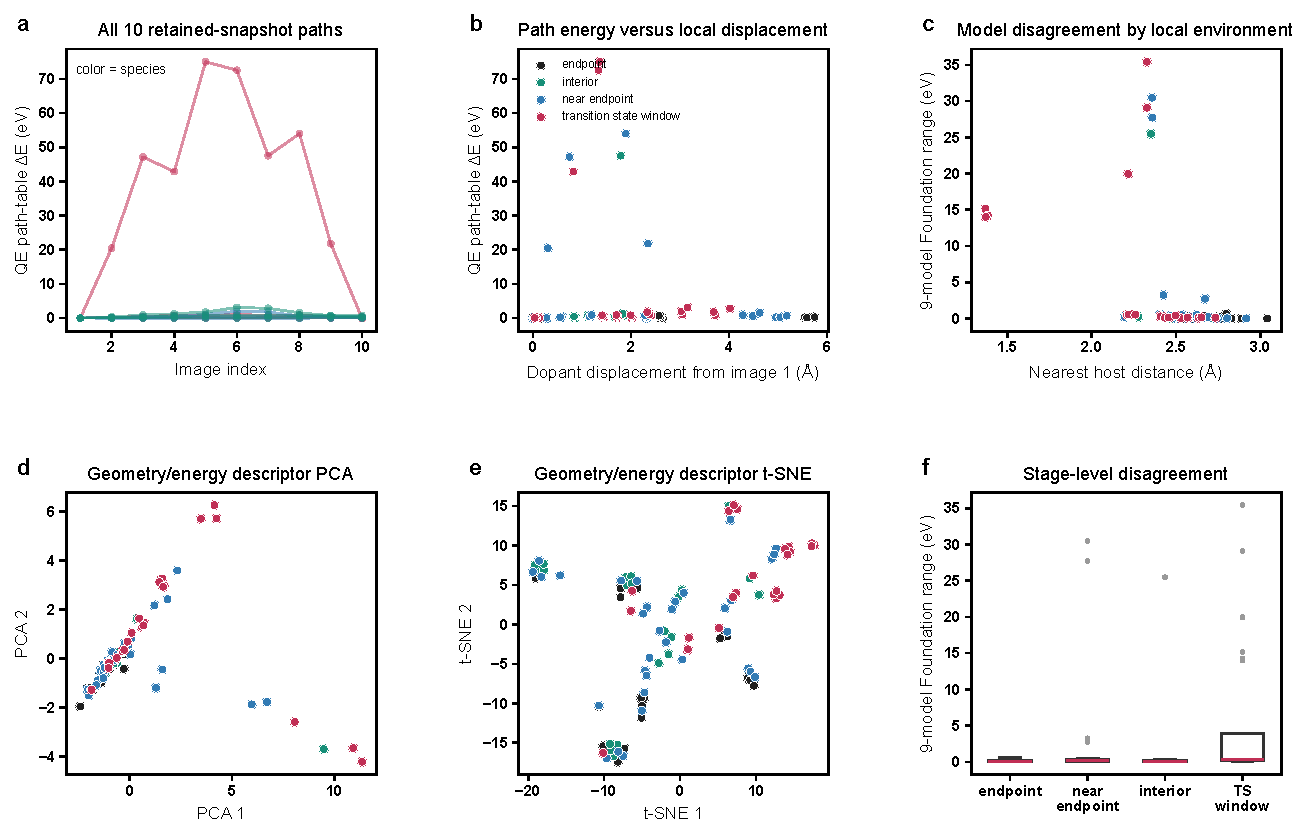
\includegraphics[width=\linewidth,height=0.42\textheight,keepaspectratio]{figure_pages/assets/fig_038.pdf}
\caption{Neb pathway, barrier, topology, or self-consistency diagnostics. This page shows the candidate output ``Figure structural stage diagnostics'' within the audited TASK3-NEB family. The panel identity, source scope, and current status are retained in the accompanying evidence matrix.}
\label{fig:candidate_038}
\end{figure}
\textbf{Results text draft.} The panels distinguish fixed-path scoring, self-consistent MLFF-NEB behavior, endpoint/path topology checks, and DFT convergence status. These operators answer different questions and are kept separate in the text.
\textbf{Discussion and boundary.} A model-reported self-relaxed barrier must not be presented as the fixed-path DFT error, and a provisional or unconverged DFT path must not be promoted to a final reference barrier.
\textbf{Article placement.} Proposed article location: Results or SI: path-family diagnostics.
\textbf{Reviewer linkage:} overall status PARTIAL.
\begin{itemize}[leftmargin=1.4em,noitemsep]
\item \textbf{REV-A1 (PARTIAL):} Reconcile Fig. 3d fixed-geometry DFT-path scoring with SI Fig. S3 self-consistent MLFF-NEB, including pathway identity and the DFT reference. \emph{Completed:} The fixed-path versus self-relaxed operator distinction and the narrower model-reported-barrier wording are integrated. \emph{Still required:} Close the restartable QE path-1--4 convergence gate, preserve the final path/source metadata, and complete the SI Fig. S3 endpoint/checkpoint/optimizer/source audit before calling the quantitative reference final.
\end{itemize}
\textbf{Evidence pointers.}
\begin{itemize}[leftmargin=1.4em,noitemsep]
\item Data/processed: \begingroup\scriptsize\url{main/analysis/task3_endpoint_only_neb/exploratory_energy_audit/all_path_structural_diagnostics/neb_descriptor_embedding.csv}\endgroup
\item Data/processed: \begingroup\scriptsize\url{main/analysis/task3_endpoint_only_neb/exploratory_energy_audit/all_path_structural_diagnostics/qe_path_stage_summary.csv}\endgroup
\item Plot/processing script: \begingroup\scriptsize\url{main/analysis/task3_endpoint_only_neb/exploratory_energy_audit/plot_paper_figures.py}\endgroup
\item Caption/text source: \begingroup\scriptsize\url{main/analysis/task3_endpoint_only_neb/exploratory_energy_audit/ACCEPTANCE_MATRIX.md}\endgroup
\item Caption/text source: \begingroup\scriptsize\url{main/analysis/task3_endpoint_only_neb/exploratory_energy_audit/EXPLORATORY_REPORT.md}\endgroup
\end{itemize}
\statusline{\textbf{Audit gap / next action:} Many per-path exports have no co-located generator; use the parent renderer and record the exact input tables}
\vfill
\clearpage
\section{FIG-039 --- Figure corrected dft foundation barrier comparison}
\label{figpage:fig-039}
\textbf{Group:} TASK3-NEB\quad \textbf{Evidence chain:} partial\quad \textbf{Status:} exploratory;audit;comparison
\begin{figure}[H]
\centering
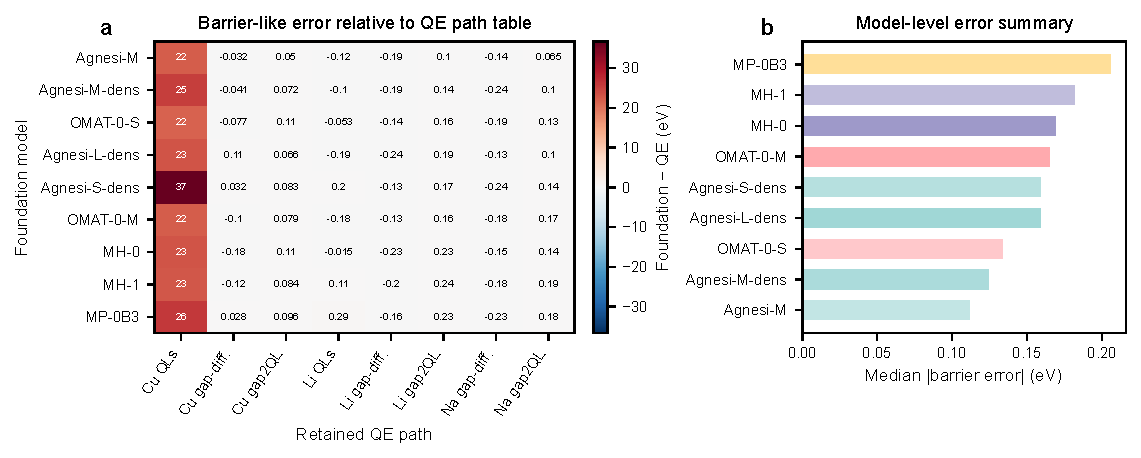
\includegraphics[width=\linewidth,height=0.42\textheight,keepaspectratio]{figure_pages/assets/fig_039.pdf}
\caption{Neb pathway, barrier, topology, or self-consistency diagnostics. This page shows the candidate output ``Figure corrected dft foundation barrier comparison'' within the audited TASK3-NEB family. The panel identity, source scope, and current status are retained in the accompanying evidence matrix.}
\label{fig:candidate_039}
\end{figure}
\textbf{Results text draft.} The panels distinguish fixed-path scoring, self-consistent MLFF-NEB behavior, endpoint/path topology checks, and DFT convergence status. These operators answer different questions and are kept separate in the text.
\textbf{Discussion and boundary.} A model-reported self-relaxed barrier must not be presented as the fixed-path DFT error, and a provisional or unconverged DFT path must not be promoted to a final reference barrier.
\textbf{Article placement.} Proposed article location: Results or SI: path-family diagnostics.
\textbf{Reviewer linkage:} overall status PARTIAL.
\begin{itemize}[leftmargin=1.4em,noitemsep]
\item \textbf{REV-A1 (PARTIAL):} Reconcile Fig. 3d fixed-geometry DFT-path scoring with SI Fig. S3 self-consistent MLFF-NEB, including pathway identity and the DFT reference. \emph{Completed:} The fixed-path versus self-relaxed operator distinction and the narrower model-reported-barrier wording are integrated. \emph{Still required:} Close the restartable QE path-1--4 convergence gate, preserve the final path/source metadata, and complete the SI Fig. S3 endpoint/checkpoint/optimizer/source audit before calling the quantitative reference final.
\end{itemize}
\textbf{Evidence pointers.}
\begin{itemize}[leftmargin=1.4em,noitemsep]
\item Data/processed: \begingroup\scriptsize\url{main/analysis/task3_endpoint_only_neb/exploratory_energy_audit/audit_summary.json}\endgroup
\item Data/processed: \begingroup\scriptsize\url{main/analysis/task3_endpoint_only_neb/exploratory_energy_audit/corrected_dft_foundation_models/corrected_dft_foundation_image_profiles.csv}\endgroup
\item Plot/processing script: \begingroup\scriptsize\url{main/analysis/task3_endpoint_only_neb/exploratory_energy_audit/plot_paper_figures.py}\endgroup
\item Caption/text source: \begingroup\scriptsize\url{main/analysis/task3_endpoint_only_neb/exploratory_energy_audit/ACCEPTANCE_MATRIX.md}\endgroup
\item Caption/text source: \begingroup\scriptsize\url{main/analysis/task3_endpoint_only_neb/exploratory_energy_audit/EXPLORATORY_REPORT.md}\endgroup
\end{itemize}
\statusline{\textbf{Audit gap / next action:} Many per-path exports have no co-located generator; use the parent renderer and record the exact input tables}
\vfill
\clearpage
\section{FIG-040 --- Figure corrected dft foundation path profiles}
\label{figpage:fig-040}
\textbf{Group:} TASK3-NEB\quad \textbf{Evidence chain:} partial\quad \textbf{Status:} exploratory;audit;comparison
\begin{figure}[H]
\centering
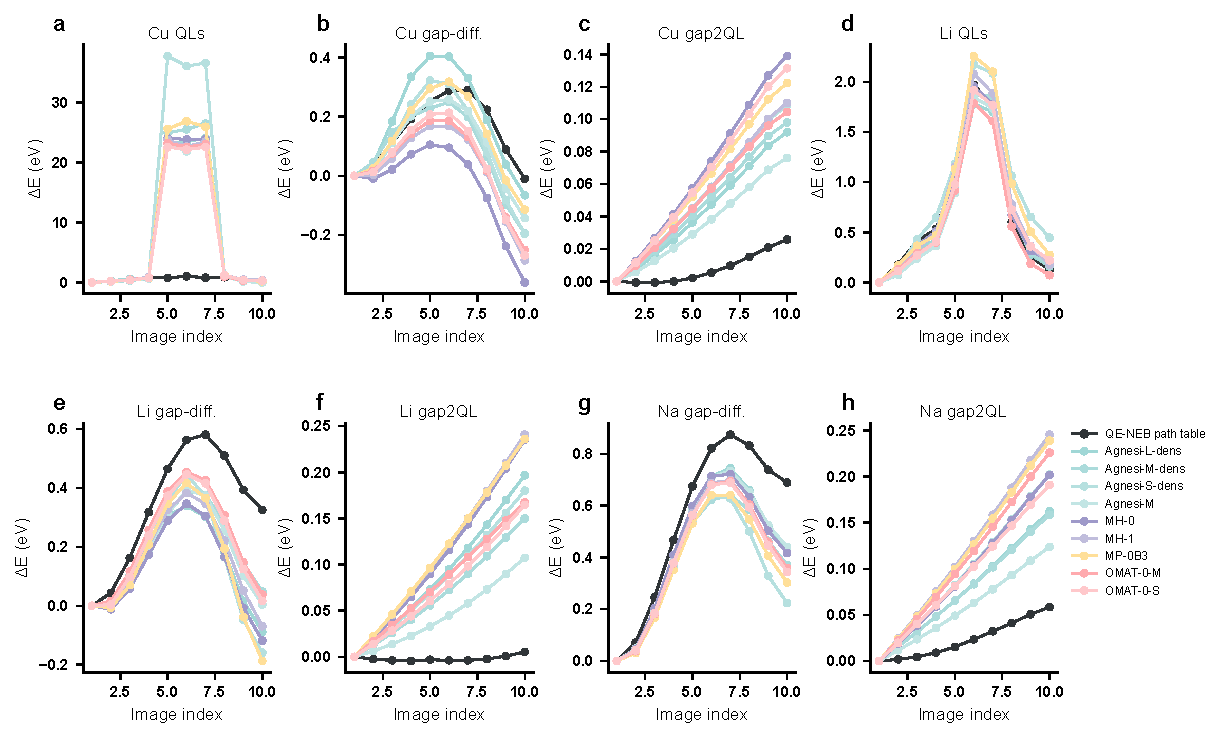
\includegraphics[width=\linewidth,height=0.42\textheight,keepaspectratio]{figure_pages/assets/fig_040.pdf}
\caption{Neb pathway, barrier, topology, or self-consistency diagnostics. This page shows the candidate output ``Figure corrected dft foundation path profiles'' within the audited TASK3-NEB family. The panel identity, source scope, and current status are retained in the accompanying evidence matrix.}
\label{fig:candidate_040}
\end{figure}
\textbf{Results text draft.} The panels distinguish fixed-path scoring, self-consistent MLFF-NEB behavior, endpoint/path topology checks, and DFT convergence status. These operators answer different questions and are kept separate in the text.
\textbf{Discussion and boundary.} A model-reported self-relaxed barrier must not be presented as the fixed-path DFT error, and a provisional or unconverged DFT path must not be promoted to a final reference barrier.
\textbf{Article placement.} Proposed article location: Results or SI: path-family diagnostics.
\textbf{Reviewer linkage:} overall status PARTIAL.
\begin{itemize}[leftmargin=1.4em,noitemsep]
\item \textbf{REV-A1 (PARTIAL):} Reconcile Fig. 3d fixed-geometry DFT-path scoring with SI Fig. S3 self-consistent MLFF-NEB, including pathway identity and the DFT reference. \emph{Completed:} The fixed-path versus self-relaxed operator distinction and the narrower model-reported-barrier wording are integrated. \emph{Still required:} Close the restartable QE path-1--4 convergence gate, preserve the final path/source metadata, and complete the SI Fig. S3 endpoint/checkpoint/optimizer/source audit before calling the quantitative reference final.
\end{itemize}
\textbf{Evidence pointers.}
\begin{itemize}[leftmargin=1.4em,noitemsep]
\item Data/processed: \begingroup\scriptsize\url{main/analysis/task3_endpoint_only_neb/exploratory_energy_audit/audit_summary.json}\endgroup
\item Data/processed: \begingroup\scriptsize\url{main/analysis/task3_endpoint_only_neb/exploratory_energy_audit/corrected_dft_foundation_models/corrected_dft_foundation_image_profiles.csv}\endgroup
\item Plot/processing script: \begingroup\scriptsize\url{main/analysis/task3_endpoint_only_neb/exploratory_energy_audit/plot_paper_figures.py}\endgroup
\item Caption/text source: \begingroup\scriptsize\url{main/analysis/task3_endpoint_only_neb/exploratory_energy_audit/ACCEPTANCE_MATRIX.md}\endgroup
\item Caption/text source: \begingroup\scriptsize\url{main/analysis/task3_endpoint_only_neb/exploratory_energy_audit/EXPLORATORY_REPORT.md}\endgroup
\end{itemize}
\statusline{\textbf{Audit gap / next action:} Many per-path exports have no co-located generator; use the parent renderer and record the exact input tables}
\vfill
\clearpage
\section{FIG-041 --- Path 1 2}
\label{figpage:fig-041}
\textbf{Group:} TASK3-NEB\quad \textbf{Evidence chain:} partial\quad \textbf{Status:} exploratory;publication;audit
\begin{figure}[H]
\centering
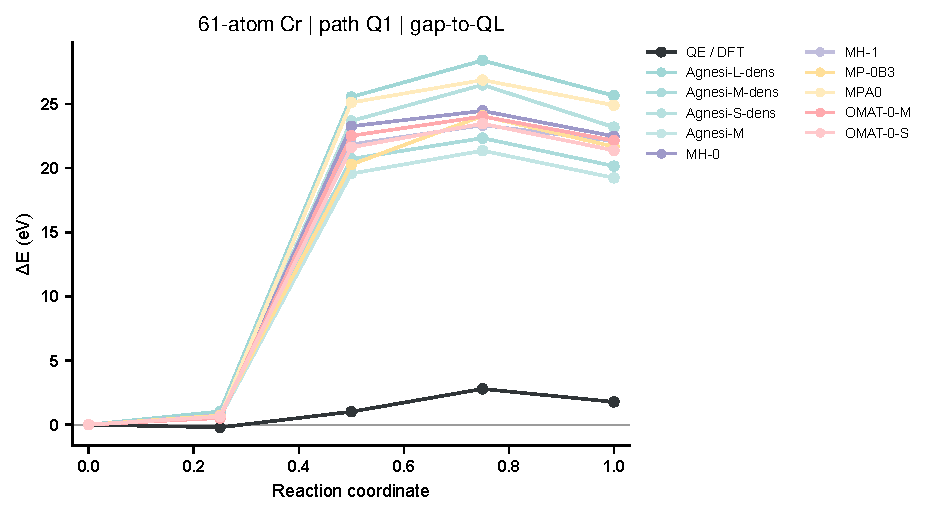
\includegraphics[width=\linewidth,height=0.42\textheight,keepaspectratio]{figure_pages/assets/fig_041.pdf}
\caption{Neb pathway, barrier, topology, or self-consistency diagnostics. This page shows the candidate output ``Path 1 2'' within the audited TASK3-NEB family. The panel identity, source scope, and current status are retained in the accompanying evidence matrix.}
\label{fig:candidate_041}
\end{figure}
\textbf{Results text draft.} The panels distinguish fixed-path scoring, self-consistent MLFF-NEB behavior, endpoint/path topology checks, and DFT convergence status. These operators answer different questions and are kept separate in the text.
\textbf{Discussion and boundary.} A model-reported self-relaxed barrier must not be presented as the fixed-path DFT error, and a provisional or unconverged DFT path must not be promoted to a final reference barrier.
\textbf{Article placement.} Proposed article location: Results or SI: path-family diagnostics.
\textbf{Reviewer linkage:} overall status PARTIAL.
\begin{itemize}[leftmargin=1.4em,noitemsep]
\item \textbf{REV-A1 (PARTIAL):} Reconcile Fig. 3d fixed-geometry DFT-path scoring with SI Fig. S3 self-consistent MLFF-NEB, including pathway identity and the DFT reference. \emph{Completed:} The fixed-path versus self-relaxed operator distinction and the narrower model-reported-barrier wording are integrated. \emph{Still required:} Close the restartable QE path-1--4 convergence gate, preserve the final path/source metadata, and complete the SI Fig. S3 endpoint/checkpoint/optimizer/source audit before calling the quantitative reference final.
\end{itemize}
\textbf{Evidence pointers.}
No data/script/text candidate was recorded in the matrix; resolve this gap before manuscript promotion.
\statusline{\textbf{Audit gap / next action:} Many per-path exports have no co-located generator; use the parent renderer and record the exact input tables}
\vfill
\clearpage
\section{FIG-042 --- Path 1 3}
\label{figpage:fig-042}
\textbf{Group:} TASK3-NEB\quad \textbf{Evidence chain:} partial\quad \textbf{Status:} exploratory;publication;audit
\begin{figure}[H]
\centering
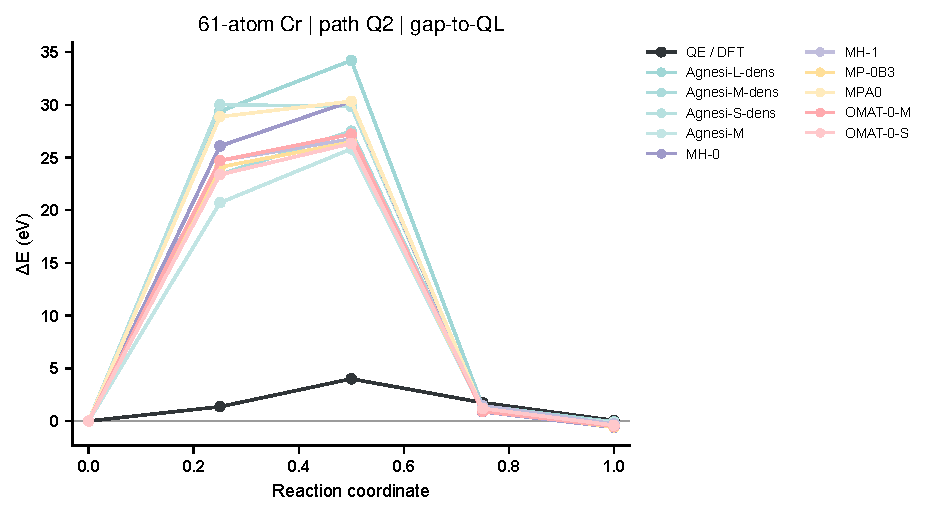
\includegraphics[width=\linewidth,height=0.42\textheight,keepaspectratio]{figure_pages/assets/fig_042.pdf}
\caption{Neb pathway, barrier, topology, or self-consistency diagnostics. This page shows the candidate output ``Path 1 3'' within the audited TASK3-NEB family. The panel identity, source scope, and current status are retained in the accompanying evidence matrix.}
\label{fig:candidate_042}
\end{figure}
\textbf{Results text draft.} The panels distinguish fixed-path scoring, self-consistent MLFF-NEB behavior, endpoint/path topology checks, and DFT convergence status. These operators answer different questions and are kept separate in the text.
\textbf{Discussion and boundary.} A model-reported self-relaxed barrier must not be presented as the fixed-path DFT error, and a provisional or unconverged DFT path must not be promoted to a final reference barrier.
\textbf{Article placement.} Proposed article location: Results or SI: path-family diagnostics.
\textbf{Reviewer linkage:} overall status PARTIAL.
\begin{itemize}[leftmargin=1.4em,noitemsep]
\item \textbf{REV-A1 (PARTIAL):} Reconcile Fig. 3d fixed-geometry DFT-path scoring with SI Fig. S3 self-consistent MLFF-NEB, including pathway identity and the DFT reference. \emph{Completed:} The fixed-path versus self-relaxed operator distinction and the narrower model-reported-barrier wording are integrated. \emph{Still required:} Close the restartable QE path-1--4 convergence gate, preserve the final path/source metadata, and complete the SI Fig. S3 endpoint/checkpoint/optimizer/source audit before calling the quantitative reference final.
\end{itemize}
\textbf{Evidence pointers.}
No data/script/text candidate was recorded in the matrix; resolve this gap before manuscript promotion.
\statusline{\textbf{Audit gap / next action:} Many per-path exports have no co-located generator; use the parent renderer and record the exact input tables}
\vfill
\clearpage
\section{FIG-043 --- Path 1 4}
\label{figpage:fig-043}
\textbf{Group:} TASK3-NEB\quad \textbf{Evidence chain:} partial\quad \textbf{Status:} exploratory;publication;audit
\begin{figure}[H]
\centering
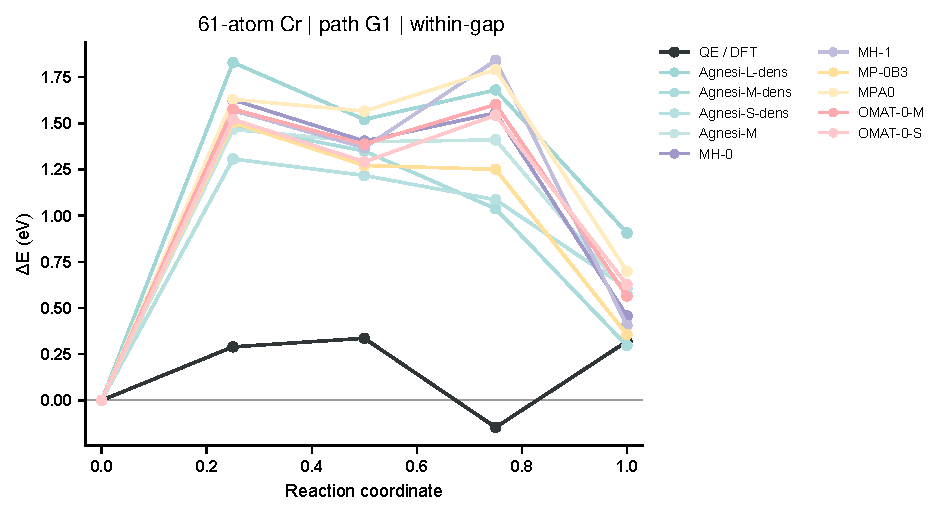
\includegraphics[width=\linewidth,height=0.42\textheight,keepaspectratio]{figure_pages/assets/fig_043.pdf}
\caption{Neb pathway, barrier, topology, or self-consistency diagnostics. This page shows the candidate output ``Path 1 4'' within the audited TASK3-NEB family. The panel identity, source scope, and current status are retained in the accompanying evidence matrix.}
\label{fig:candidate_043}
\end{figure}
\textbf{Results text draft.} The panels distinguish fixed-path scoring, self-consistent MLFF-NEB behavior, endpoint/path topology checks, and DFT convergence status. These operators answer different questions and are kept separate in the text.
\textbf{Discussion and boundary.} A model-reported self-relaxed barrier must not be presented as the fixed-path DFT error, and a provisional or unconverged DFT path must not be promoted to a final reference barrier.
\textbf{Article placement.} Proposed article location: Results or SI: path-family diagnostics.
\textbf{Reviewer linkage:} overall status PARTIAL.
\begin{itemize}[leftmargin=1.4em,noitemsep]
\item \textbf{REV-A1 (PARTIAL):} Reconcile Fig. 3d fixed-geometry DFT-path scoring with SI Fig. S3 self-consistent MLFF-NEB, including pathway identity and the DFT reference. \emph{Completed:} The fixed-path versus self-relaxed operator distinction and the narrower model-reported-barrier wording are integrated. \emph{Still required:} Close the restartable QE path-1--4 convergence gate, preserve the final path/source metadata, and complete the SI Fig. S3 endpoint/checkpoint/optimizer/source audit before calling the quantitative reference final.
\end{itemize}
\textbf{Evidence pointers.}
No data/script/text candidate was recorded in the matrix; resolve this gap before manuscript promotion.
\statusline{\textbf{Audit gap / next action:} Many per-path exports have no co-located generator; use the parent renderer and record the exact input tables}
\vfill
\clearpage
\section{FIG-044 --- Path 1 5}
\label{figpage:fig-044}
\textbf{Group:} TASK3-NEB\quad \textbf{Evidence chain:} partial\quad \textbf{Status:} exploratory;publication;audit
\begin{figure}[H]
\centering
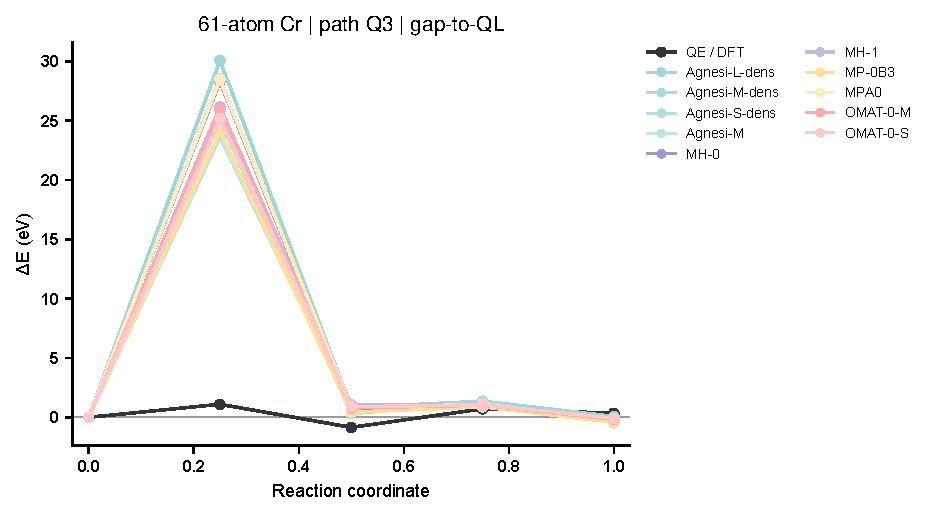
\includegraphics[width=\linewidth,height=0.42\textheight,keepaspectratio]{figure_pages/assets/fig_044.pdf}
\caption{Neb pathway, barrier, topology, or self-consistency diagnostics. This page shows the candidate output ``Path 1 5'' within the audited TASK3-NEB family. The panel identity, source scope, and current status are retained in the accompanying evidence matrix.}
\label{fig:candidate_044}
\end{figure}
\textbf{Results text draft.} The panels distinguish fixed-path scoring, self-consistent MLFF-NEB behavior, endpoint/path topology checks, and DFT convergence status. These operators answer different questions and are kept separate in the text.
\textbf{Discussion and boundary.} A model-reported self-relaxed barrier must not be presented as the fixed-path DFT error, and a provisional or unconverged DFT path must not be promoted to a final reference barrier.
\textbf{Article placement.} Proposed article location: Results or SI: path-family diagnostics.
\textbf{Reviewer linkage:} overall status PARTIAL.
\begin{itemize}[leftmargin=1.4em,noitemsep]
\item \textbf{REV-A1 (PARTIAL):} Reconcile Fig. 3d fixed-geometry DFT-path scoring with SI Fig. S3 self-consistent MLFF-NEB, including pathway identity and the DFT reference. \emph{Completed:} The fixed-path versus self-relaxed operator distinction and the narrower model-reported-barrier wording are integrated. \emph{Still required:} Close the restartable QE path-1--4 convergence gate, preserve the final path/source metadata, and complete the SI Fig. S3 endpoint/checkpoint/optimizer/source audit before calling the quantitative reference final.
\end{itemize}
\textbf{Evidence pointers.}
No data/script/text candidate was recorded in the matrix; resolve this gap before manuscript promotion.
\statusline{\textbf{Audit gap / next action:} Many per-path exports have no co-located generator; use the parent renderer and record the exact input tables}
\vfill
\clearpage
\section{FIG-045 --- Path 1 7}
\label{figpage:fig-045}
\textbf{Group:} TASK3-NEB\quad \textbf{Evidence chain:} partial\quad \textbf{Status:} exploratory;publication;audit
\begin{figure}[H]
\centering
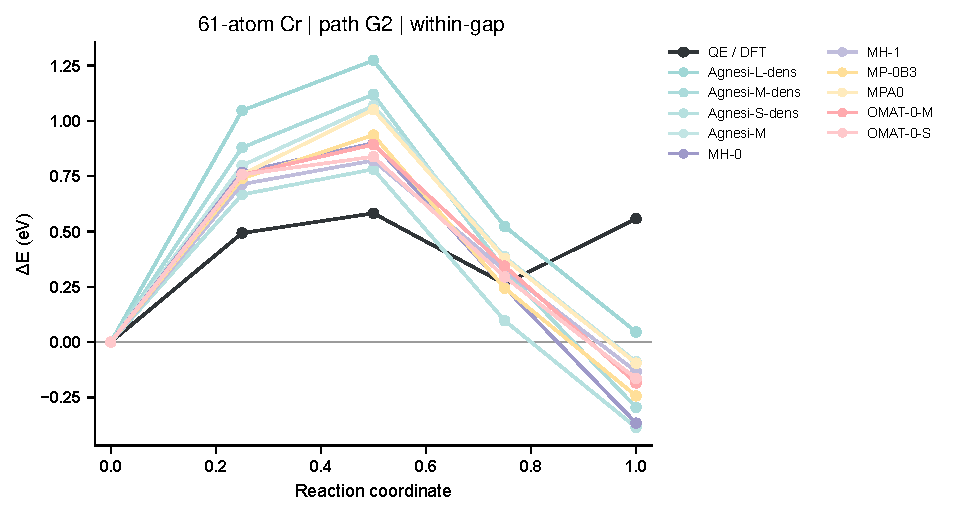
\includegraphics[width=\linewidth,height=0.42\textheight,keepaspectratio]{figure_pages/assets/fig_045.pdf}
\caption{Neb pathway, barrier, topology, or self-consistency diagnostics. This page shows the candidate output ``Path 1 7'' within the audited TASK3-NEB family. The panel identity, source scope, and current status are retained in the accompanying evidence matrix.}
\label{fig:candidate_045}
\end{figure}
\textbf{Results text draft.} The panels distinguish fixed-path scoring, self-consistent MLFF-NEB behavior, endpoint/path topology checks, and DFT convergence status. These operators answer different questions and are kept separate in the text.
\textbf{Discussion and boundary.} A model-reported self-relaxed barrier must not be presented as the fixed-path DFT error, and a provisional or unconverged DFT path must not be promoted to a final reference barrier.
\textbf{Article placement.} Proposed article location: Results or SI: path-family diagnostics.
\textbf{Reviewer linkage:} overall status PARTIAL.
\begin{itemize}[leftmargin=1.4em,noitemsep]
\item \textbf{REV-A1 (PARTIAL):} Reconcile Fig. 3d fixed-geometry DFT-path scoring with SI Fig. S3 self-consistent MLFF-NEB, including pathway identity and the DFT reference. \emph{Completed:} The fixed-path versus self-relaxed operator distinction and the narrower model-reported-barrier wording are integrated. \emph{Still required:} Close the restartable QE path-1--4 convergence gate, preserve the final path/source metadata, and complete the SI Fig. S3 endpoint/checkpoint/optimizer/source audit before calling the quantitative reference final.
\end{itemize}
\textbf{Evidence pointers.}
No data/script/text candidate was recorded in the matrix; resolve this gap before manuscript promotion.
\statusline{\textbf{Audit gap / next action:} Many per-path exports have no co-located generator; use the parent renderer and record the exact input tables}
\vfill
\clearpage
\section{FIG-046 --- Path neb 1}
\label{figpage:fig-046}
\textbf{Group:} TASK3-NEB\quad \textbf{Evidence chain:} partial\quad \textbf{Status:} exploratory;publication;audit
\begin{figure}[H]
\centering
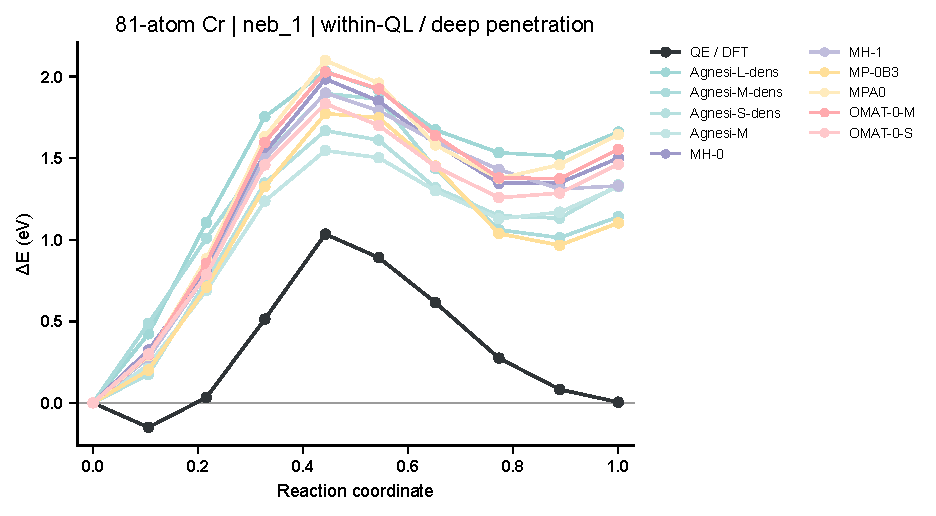
\includegraphics[width=\linewidth,height=0.42\textheight,keepaspectratio]{figure_pages/assets/fig_046.pdf}
\caption{Neb pathway, barrier, topology, or self-consistency diagnostics. This page shows the candidate output ``Path neb 1'' within the audited TASK3-NEB family. The panel identity, source scope, and current status are retained in the accompanying evidence matrix.}
\label{fig:candidate_046}
\end{figure}
\textbf{Results text draft.} The panels distinguish fixed-path scoring, self-consistent MLFF-NEB behavior, endpoint/path topology checks, and DFT convergence status. These operators answer different questions and are kept separate in the text.
\textbf{Discussion and boundary.} A model-reported self-relaxed barrier must not be presented as the fixed-path DFT error, and a provisional or unconverged DFT path must not be promoted to a final reference barrier.
\textbf{Article placement.} Proposed article location: Results or SI: path-family diagnostics.
\textbf{Reviewer linkage:} overall status PARTIAL.
\begin{itemize}[leftmargin=1.4em,noitemsep]
\item \textbf{REV-A1 (PARTIAL):} Reconcile Fig. 3d fixed-geometry DFT-path scoring with SI Fig. S3 self-consistent MLFF-NEB, including pathway identity and the DFT reference. \emph{Completed:} The fixed-path versus self-relaxed operator distinction and the narrower model-reported-barrier wording are integrated. \emph{Still required:} Close the restartable QE path-1--4 convergence gate, preserve the final path/source metadata, and complete the SI Fig. S3 endpoint/checkpoint/optimizer/source audit before calling the quantitative reference final.
\end{itemize}
\textbf{Evidence pointers.}
No data/script/text candidate was recorded in the matrix; resolve this gap before manuscript promotion.
\statusline{\textbf{Audit gap / next action:} Many per-path exports have no co-located generator; use the parent renderer and record the exact input tables}
\vfill
\clearpage
\section{FIG-047 --- Path neb 2}
\label{figpage:fig-047}
\textbf{Group:} TASK3-NEB\quad \textbf{Evidence chain:} partial\quad \textbf{Status:} exploratory;publication;audit
\begin{figure}[H]
\centering
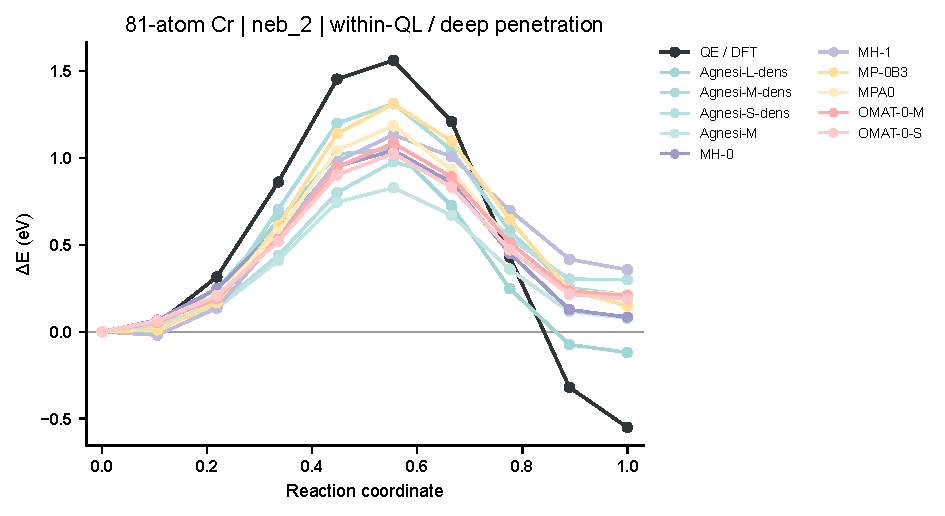
\includegraphics[width=\linewidth,height=0.42\textheight,keepaspectratio]{figure_pages/assets/fig_047.pdf}
\caption{Neb pathway, barrier, topology, or self-consistency diagnostics. This page shows the candidate output ``Path neb 2'' within the audited TASK3-NEB family. The panel identity, source scope, and current status are retained in the accompanying evidence matrix.}
\label{fig:candidate_047}
\end{figure}
\textbf{Results text draft.} The panels distinguish fixed-path scoring, self-consistent MLFF-NEB behavior, endpoint/path topology checks, and DFT convergence status. These operators answer different questions and are kept separate in the text.
\textbf{Discussion and boundary.} A model-reported self-relaxed barrier must not be presented as the fixed-path DFT error, and a provisional or unconverged DFT path must not be promoted to a final reference barrier.
\textbf{Article placement.} Proposed article location: Results or SI: path-family diagnostics.
\textbf{Reviewer linkage:} overall status PARTIAL.
\begin{itemize}[leftmargin=1.4em,noitemsep]
\item \textbf{REV-A1 (PARTIAL):} Reconcile Fig. 3d fixed-geometry DFT-path scoring with SI Fig. S3 self-consistent MLFF-NEB, including pathway identity and the DFT reference. \emph{Completed:} The fixed-path versus self-relaxed operator distinction and the narrower model-reported-barrier wording are integrated. \emph{Still required:} Close the restartable QE path-1--4 convergence gate, preserve the final path/source metadata, and complete the SI Fig. S3 endpoint/checkpoint/optimizer/source audit before calling the quantitative reference final.
\end{itemize}
\textbf{Evidence pointers.}
No data/script/text candidate was recorded in the matrix; resolve this gap before manuscript promotion.
\statusline{\textbf{Audit gap / next action:} Many per-path exports have no co-located generator; use the parent renderer and record the exact input tables}
\vfill
\clearpage
\section{FIG-048 --- Path neb 3}
\label{figpage:fig-048}
\textbf{Group:} TASK3-NEB\quad \textbf{Evidence chain:} partial\quad \textbf{Status:} exploratory;publication;audit
\begin{figure}[H]
\centering
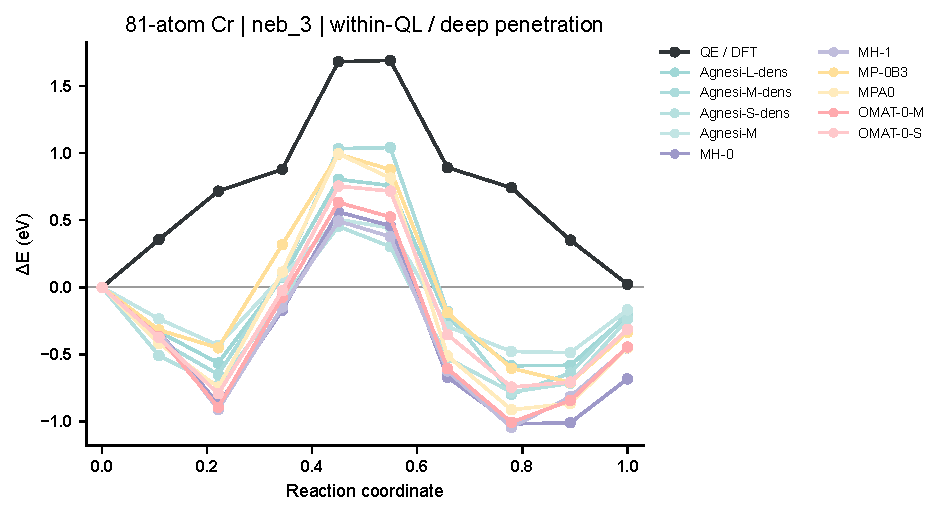
\includegraphics[width=\linewidth,height=0.42\textheight,keepaspectratio]{figure_pages/assets/fig_048.pdf}
\caption{Neb pathway, barrier, topology, or self-consistency diagnostics. This page shows the candidate output ``Path neb 3'' within the audited TASK3-NEB family. The panel identity, source scope, and current status are retained in the accompanying evidence matrix.}
\label{fig:candidate_048}
\end{figure}
\textbf{Results text draft.} The panels distinguish fixed-path scoring, self-consistent MLFF-NEB behavior, endpoint/path topology checks, and DFT convergence status. These operators answer different questions and are kept separate in the text.
\textbf{Discussion and boundary.} A model-reported self-relaxed barrier must not be presented as the fixed-path DFT error, and a provisional or unconverged DFT path must not be promoted to a final reference barrier.
\textbf{Article placement.} Proposed article location: Results or SI: path-family diagnostics.
\textbf{Reviewer linkage:} overall status PARTIAL.
\begin{itemize}[leftmargin=1.4em,noitemsep]
\item \textbf{REV-A1 (PARTIAL):} Reconcile Fig. 3d fixed-geometry DFT-path scoring with SI Fig. S3 self-consistent MLFF-NEB, including pathway identity and the DFT reference. \emph{Completed:} The fixed-path versus self-relaxed operator distinction and the narrower model-reported-barrier wording are integrated. \emph{Still required:} Close the restartable QE path-1--4 convergence gate, preserve the final path/source metadata, and complete the SI Fig. S3 endpoint/checkpoint/optimizer/source audit before calling the quantitative reference final.
\end{itemize}
\textbf{Evidence pointers.}
No data/script/text candidate was recorded in the matrix; resolve this gap before manuscript promotion.
\statusline{\textbf{Audit gap / next action:} Many per-path exports have no co-located generator; use the parent renderer and record the exact input tables}
\vfill
\clearpage
\section{FIG-049 --- Path neb 4}
\label{figpage:fig-049}
\textbf{Group:} TASK3-NEB\quad \textbf{Evidence chain:} partial\quad \textbf{Status:} exploratory;publication;audit
\begin{figure}[H]
\centering
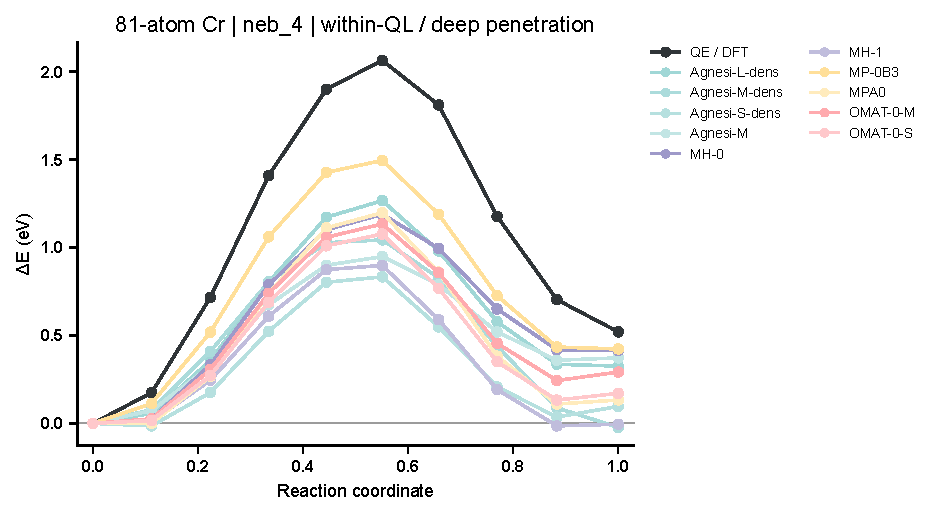
\includegraphics[width=\linewidth,height=0.42\textheight,keepaspectratio]{figure_pages/assets/fig_049.pdf}
\caption{Neb pathway, barrier, topology, or self-consistency diagnostics. This page shows the candidate output ``Path neb 4'' within the audited TASK3-NEB family. The panel identity, source scope, and current status are retained in the accompanying evidence matrix.}
\label{fig:candidate_049}
\end{figure}
\textbf{Results text draft.} The panels distinguish fixed-path scoring, self-consistent MLFF-NEB behavior, endpoint/path topology checks, and DFT convergence status. These operators answer different questions and are kept separate in the text.
\textbf{Discussion and boundary.} A model-reported self-relaxed barrier must not be presented as the fixed-path DFT error, and a provisional or unconverged DFT path must not be promoted to a final reference barrier.
\textbf{Article placement.} Proposed article location: Results or SI: path-family diagnostics.
\textbf{Reviewer linkage:} overall status PARTIAL.
\begin{itemize}[leftmargin=1.4em,noitemsep]
\item \textbf{REV-A1 (PARTIAL):} Reconcile Fig. 3d fixed-geometry DFT-path scoring with SI Fig. S3 self-consistent MLFF-NEB, including pathway identity and the DFT reference. \emph{Completed:} The fixed-path versus self-relaxed operator distinction and the narrower model-reported-barrier wording are integrated. \emph{Still required:} Close the restartable QE path-1--4 convergence gate, preserve the final path/source metadata, and complete the SI Fig. S3 endpoint/checkpoint/optimizer/source audit before calling the quantitative reference final.
\end{itemize}
\textbf{Evidence pointers.}
No data/script/text candidate was recorded in the matrix; resolve this gap before manuscript promotion.
\statusline{\textbf{Audit gap / next action:} Many per-path exports have no co-located generator; use the parent renderer and record the exact input tables}
\vfill
\clearpage
\section{FIG-050 --- Path neb 5}
\label{figpage:fig-050}
\textbf{Group:} TASK3-NEB\quad \textbf{Evidence chain:} partial\quad \textbf{Status:} exploratory;publication;audit
\begin{figure}[H]
\centering
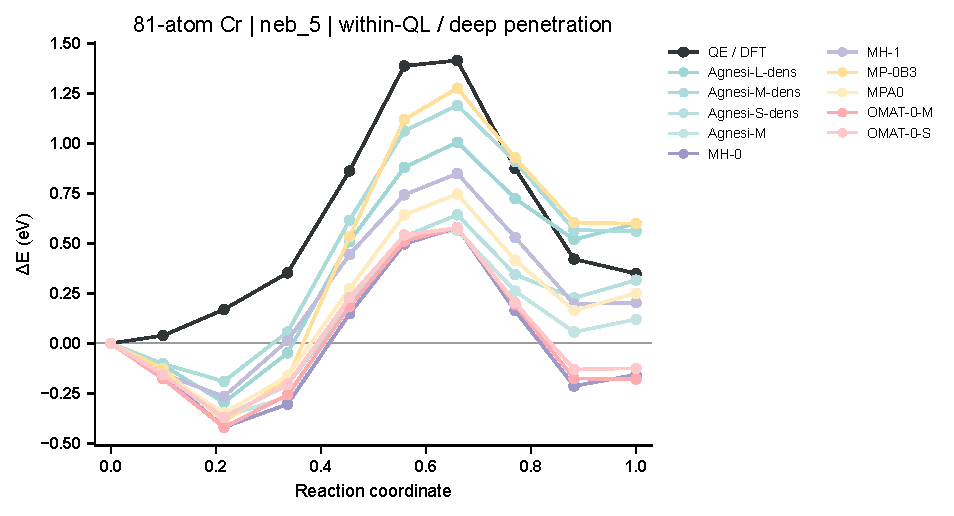
\includegraphics[width=\linewidth,height=0.42\textheight,keepaspectratio]{figure_pages/assets/fig_050.pdf}
\caption{Neb pathway, barrier, topology, or self-consistency diagnostics. This page shows the candidate output ``Path neb 5'' within the audited TASK3-NEB family. The panel identity, source scope, and current status are retained in the accompanying evidence matrix.}
\label{fig:candidate_050}
\end{figure}
\textbf{Results text draft.} The panels distinguish fixed-path scoring, self-consistent MLFF-NEB behavior, endpoint/path topology checks, and DFT convergence status. These operators answer different questions and are kept separate in the text.
\textbf{Discussion and boundary.} A model-reported self-relaxed barrier must not be presented as the fixed-path DFT error, and a provisional or unconverged DFT path must not be promoted to a final reference barrier.
\textbf{Article placement.} Proposed article location: Results or SI: path-family diagnostics.
\textbf{Reviewer linkage:} overall status PARTIAL.
\begin{itemize}[leftmargin=1.4em,noitemsep]
\item \textbf{REV-A1 (PARTIAL):} Reconcile Fig. 3d fixed-geometry DFT-path scoring with SI Fig. S3 self-consistent MLFF-NEB, including pathway identity and the DFT reference. \emph{Completed:} The fixed-path versus self-relaxed operator distinction and the narrower model-reported-barrier wording are integrated. \emph{Still required:} Close the restartable QE path-1--4 convergence gate, preserve the final path/source metadata, and complete the SI Fig. S3 endpoint/checkpoint/optimizer/source audit before calling the quantitative reference final.
\end{itemize}
\textbf{Evidence pointers.}
No data/script/text candidate was recorded in the matrix; resolve this gap before manuscript promotion.
\statusline{\textbf{Audit gap / next action:} Many per-path exports have no co-located generator; use the parent renderer and record the exact input tables}
\vfill
\clearpage
\section{FIG-051 --- Figure cr61 cr81 geometry embedding}
\label{figpage:fig-051}
\textbf{Group:} TASK3-NEB\quad \textbf{Evidence chain:} partial\quad \textbf{Status:} exploratory;publication;audit
\begin{figure}[H]
\centering
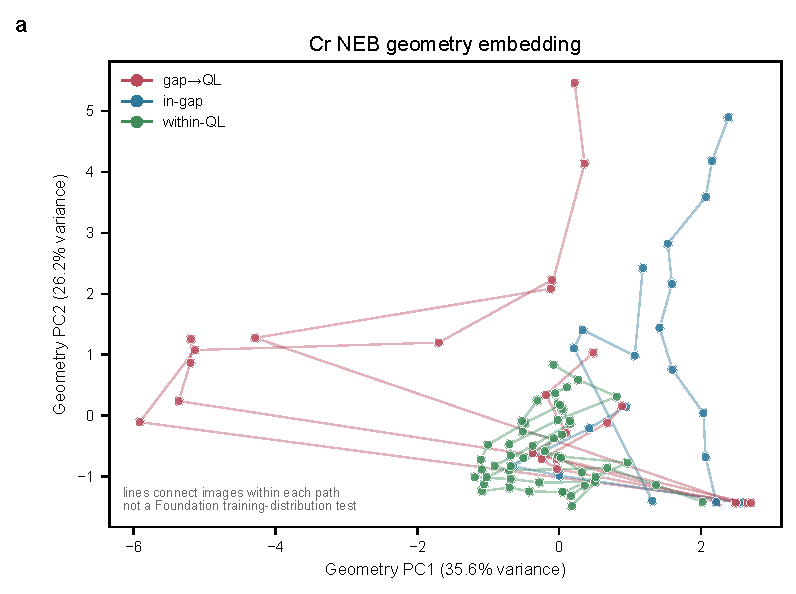
\includegraphics[width=\linewidth,height=0.42\textheight,keepaspectratio]{figure_pages/assets/fig_051.pdf}
\caption{Neb pathway, barrier, topology, or self-consistency diagnostics. This page shows the candidate output ``Figure cr61 cr81 geometry embedding'' within the audited TASK3-NEB family. The panel identity, source scope, and current status are retained in the accompanying evidence matrix.}
\label{fig:candidate_051}
\end{figure}
\textbf{Results text draft.} The panels distinguish fixed-path scoring, self-consistent MLFF-NEB behavior, endpoint/path topology checks, and DFT convergence status. These operators answer different questions and are kept separate in the text.
\textbf{Discussion and boundary.} A model-reported self-relaxed barrier must not be presented as the fixed-path DFT error, and a provisional or unconverged DFT path must not be promoted to a final reference barrier.
\textbf{Article placement.} Proposed article location: Results or SI: path-family diagnostics.
\textbf{Reviewer linkage:} overall status PARTIAL.
\begin{itemize}[leftmargin=1.4em,noitemsep]
\item \textbf{REV-A1 (PARTIAL):} Reconcile Fig. 3d fixed-geometry DFT-path scoring with SI Fig. S3 self-consistent MLFF-NEB, including pathway identity and the DFT reference. \emph{Completed:} The fixed-path versus self-relaxed operator distinction and the narrower model-reported-barrier wording are integrated. \emph{Still required:} Close the restartable QE path-1--4 convergence gate, preserve the final path/source metadata, and complete the SI Fig. S3 endpoint/checkpoint/optimizer/source audit before calling the quantitative reference final.
\end{itemize}
\textbf{Evidence pointers.}
\begin{itemize}[leftmargin=1.4em,noitemsep]
\item Data/processed: \begingroup\scriptsize\url{main/analysis/task3_endpoint_only_neb/exploratory_energy_audit/cr_61_81_three_class_20261003/61_atom_geometry_classification.csv}\endgroup
\item Data/processed: \begingroup\scriptsize\url{main/analysis/task3_endpoint_only_neb/exploratory_energy_audit/cr_61_81_three_class_20261003/61_atom_geometry_classification.json}\endgroup
\item Caption/text source: \begingroup\scriptsize\url{main/analysis/task3_endpoint_only_neb/exploratory_energy_audit/cr_61_81_three_class_20261003/Cr61_Cr81_foundation_comparison_report.md}\endgroup
\item Caption/text source: \begingroup\scriptsize\url{main/analysis/task3_endpoint_only_neb/exploratory_energy_audit/cr_61_81_three_class_20261003/Cr61_Cr81_publication_acceptance_matrix.tex}\endgroup
\end{itemize}
\statusline{\textbf{Audit gap / next action:} Many per-path exports have no co-located generator; use the parent renderer and record the exact input tables}
\vfill
\clearpage
\section{FIG-052 --- Figure cr61 cr81 unified diagnostic framework}
\label{figpage:fig-052}
\textbf{Group:} TASK3-NEB\quad \textbf{Evidence chain:} partial\quad \textbf{Status:} exploratory;publication;audit
\begin{figure}[H]
\centering
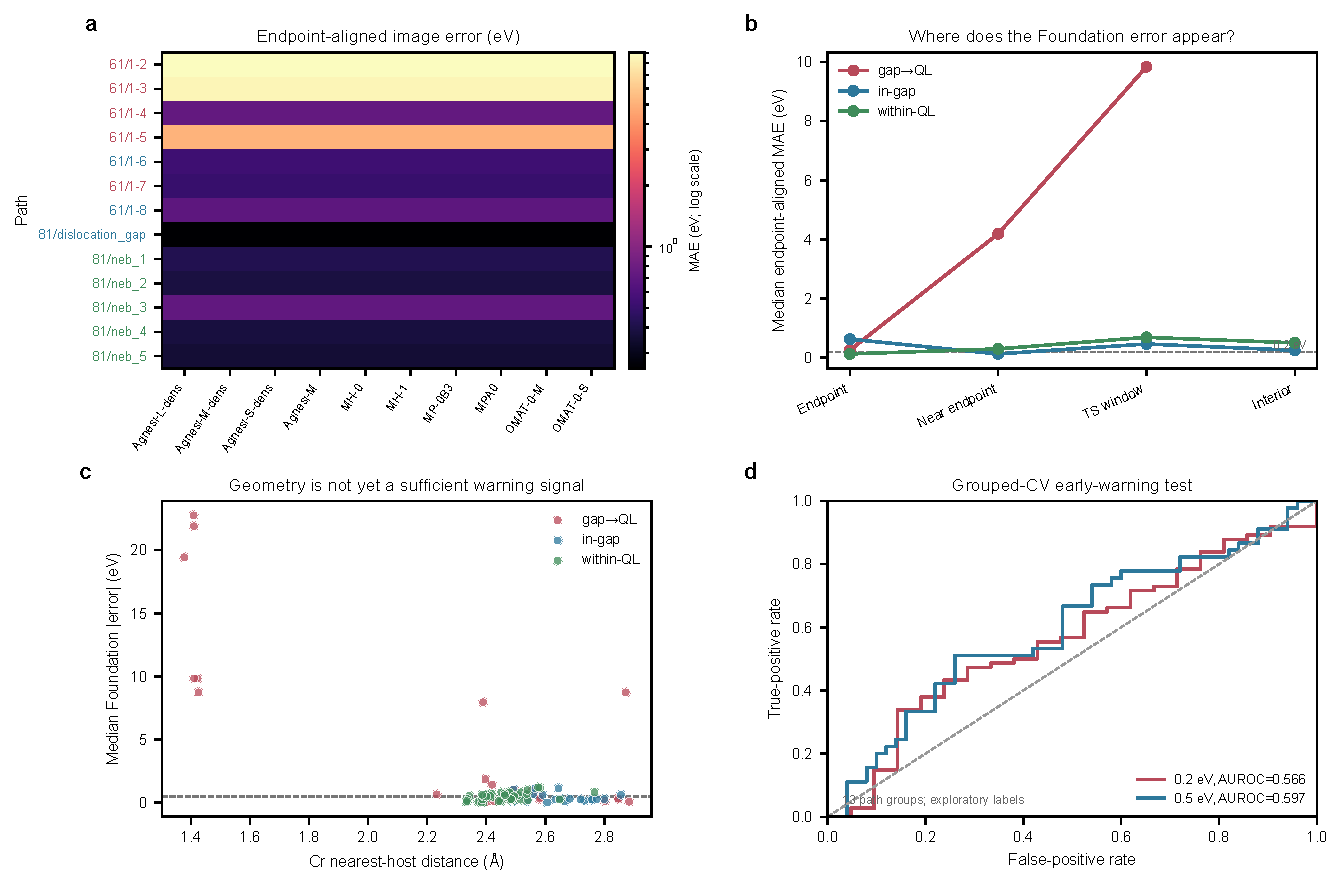
\includegraphics[width=\linewidth,height=0.42\textheight,keepaspectratio]{figure_pages/assets/fig_052.pdf}
\caption{Neb pathway, barrier, topology, or self-consistency diagnostics. This page shows the candidate output ``Figure cr61 cr81 unified diagnostic framework'' within the audited TASK3-NEB family. The panel identity, source scope, and current status are retained in the accompanying evidence matrix.}
\label{fig:candidate_052}
\end{figure}
\textbf{Results text draft.} The panels distinguish fixed-path scoring, self-consistent MLFF-NEB behavior, endpoint/path topology checks, and DFT convergence status. These operators answer different questions and are kept separate in the text.
\textbf{Discussion and boundary.} A model-reported self-relaxed barrier must not be presented as the fixed-path DFT error, and a provisional or unconverged DFT path must not be promoted to a final reference barrier.
\textbf{Article placement.} Proposed article location: Results or SI: path-family diagnostics.
\textbf{Reviewer linkage:} overall status PARTIAL.
\begin{itemize}[leftmargin=1.4em,noitemsep]
\item \textbf{REV-A1 (PARTIAL):} Reconcile Fig. 3d fixed-geometry DFT-path scoring with SI Fig. S3 self-consistent MLFF-NEB, including pathway identity and the DFT reference. \emph{Completed:} The fixed-path versus self-relaxed operator distinction and the narrower model-reported-barrier wording are integrated. \emph{Still required:} Close the restartable QE path-1--4 convergence gate, preserve the final path/source metadata, and complete the SI Fig. S3 endpoint/checkpoint/optimizer/source audit before calling the quantitative reference final.
\end{itemize}
\textbf{Evidence pointers.}
\begin{itemize}[leftmargin=1.4em,noitemsep]
\item Data/processed: \begingroup\scriptsize\url{main/analysis/task3_endpoint_only_neb/exploratory_energy_audit/cr_61_81_three_class_20261003/61_atom_geometry_classification.csv}\endgroup
\item Data/processed: \begingroup\scriptsize\url{main/analysis/task3_endpoint_only_neb/exploratory_energy_audit/cr_61_81_three_class_20261003/61_atom_geometry_classification.json}\endgroup
\item Caption/text source: \begingroup\scriptsize\url{main/analysis/task3_endpoint_only_neb/exploratory_energy_audit/cr_61_81_three_class_20261003/Cr61_Cr81_foundation_comparison_report.md}\endgroup
\item Caption/text source: \begingroup\scriptsize\url{main/analysis/task3_endpoint_only_neb/exploratory_energy_audit/cr_61_81_three_class_20261003/Cr61_Cr81_publication_acceptance_matrix.tex}\endgroup
\end{itemize}
\statusline{\textbf{Audit gap / next action:} Many per-path exports have no co-located generator; use the parent renderer and record the exact input tables}
\vfill
\clearpage
\section{FIG-053 --- Figure cr61 gap to ql all foundation profiles}
\label{figpage:fig-053}
\textbf{Group:} TASK3-NEB\quad \textbf{Evidence chain:} partial\quad \textbf{Status:} exploratory;publication;audit;comparison
\begin{figure}[H]
\centering
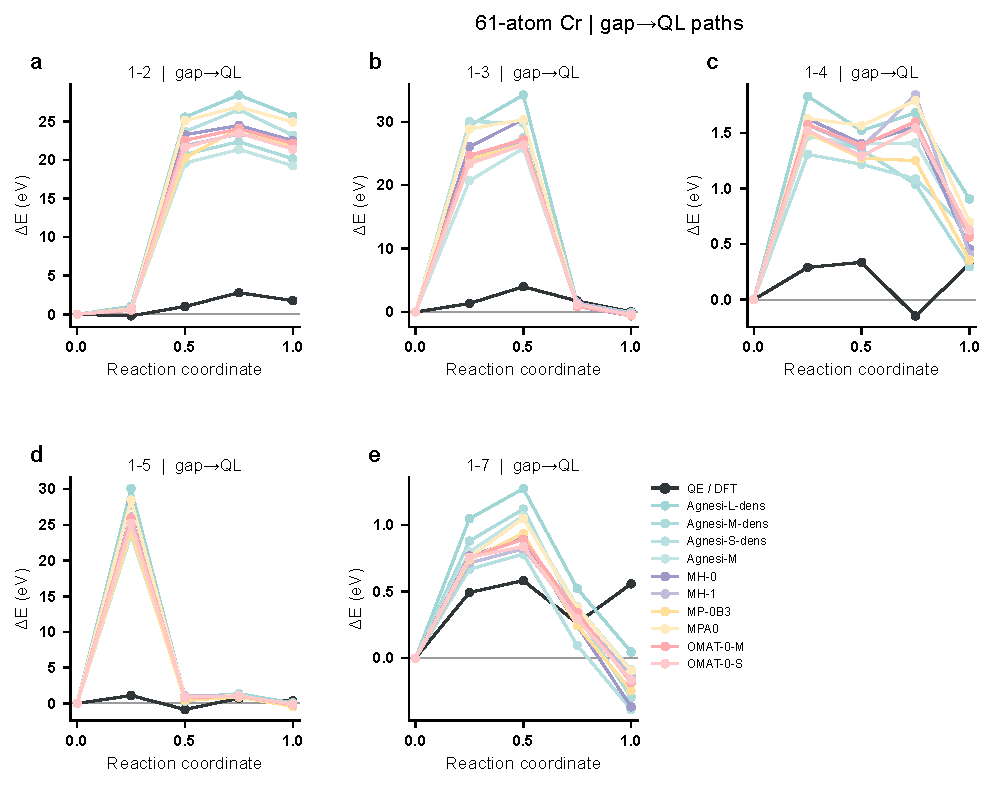
\includegraphics[width=\linewidth,height=0.42\textheight,keepaspectratio]{figure_pages/assets/fig_053.pdf}
\caption{Neb pathway, barrier, topology, or self-consistency diagnostics. This page shows the candidate output ``Figure cr61 gap to ql all foundation profiles'' within the audited TASK3-NEB family. The panel identity, source scope, and current status are retained in the accompanying evidence matrix.}
\label{fig:candidate_053}
\end{figure}
\textbf{Results text draft.} The panels distinguish fixed-path scoring, self-consistent MLFF-NEB behavior, endpoint/path topology checks, and DFT convergence status. These operators answer different questions and are kept separate in the text.
\textbf{Discussion and boundary.} A model-reported self-relaxed barrier must not be presented as the fixed-path DFT error, and a provisional or unconverged DFT path must not be promoted to a final reference barrier.
\textbf{Article placement.} Proposed article location: Results or SI: path-family diagnostics.
\textbf{Reviewer linkage:} overall status PARTIAL.
\begin{itemize}[leftmargin=1.4em,noitemsep]
\item \textbf{REV-A1 (PARTIAL):} Reconcile Fig. 3d fixed-geometry DFT-path scoring with SI Fig. S3 self-consistent MLFF-NEB, including pathway identity and the DFT reference. \emph{Completed:} The fixed-path versus self-relaxed operator distinction and the narrower model-reported-barrier wording are integrated. \emph{Still required:} Close the restartable QE path-1--4 convergence gate, preserve the final path/source metadata, and complete the SI Fig. S3 endpoint/checkpoint/optimizer/source audit before calling the quantitative reference final.
\end{itemize}
\textbf{Evidence pointers.}
\begin{itemize}[leftmargin=1.4em,noitemsep]
\item Data/processed: \begingroup\scriptsize\url{main/analysis/task3_endpoint_only_neb/exploratory_energy_audit/cr_61_81_three_class_20261003/61_atom_geometry_classification.csv}\endgroup
\item Data/processed: \begingroup\scriptsize\url{main/analysis/task3_endpoint_only_neb/exploratory_energy_audit/cr_61_81_three_class_20261003/61_atom_geometry_classification.json}\endgroup
\item Caption/text source: \begingroup\scriptsize\url{main/analysis/task3_endpoint_only_neb/exploratory_energy_audit/cr_61_81_three_class_20261003/Cr61_Cr81_foundation_comparison_report.md}\endgroup
\item Caption/text source: \begingroup\scriptsize\url{main/analysis/task3_endpoint_only_neb/exploratory_energy_audit/cr_61_81_three_class_20261003/Cr61_Cr81_publication_acceptance_matrix.tex}\endgroup
\end{itemize}
\statusline{\textbf{Audit gap / next action:} Many per-path exports have no co-located generator; use the parent renderer and record the exact input tables}
\vfill
\clearpage
\section{FIG-054 --- Figure cr81 grouped all foundation profiles}
\label{figpage:fig-054}
\textbf{Group:} TASK3-NEB\quad \textbf{Evidence chain:} partial\quad \textbf{Status:} exploratory;publication;audit;comparison
\begin{figure}[H]
\centering
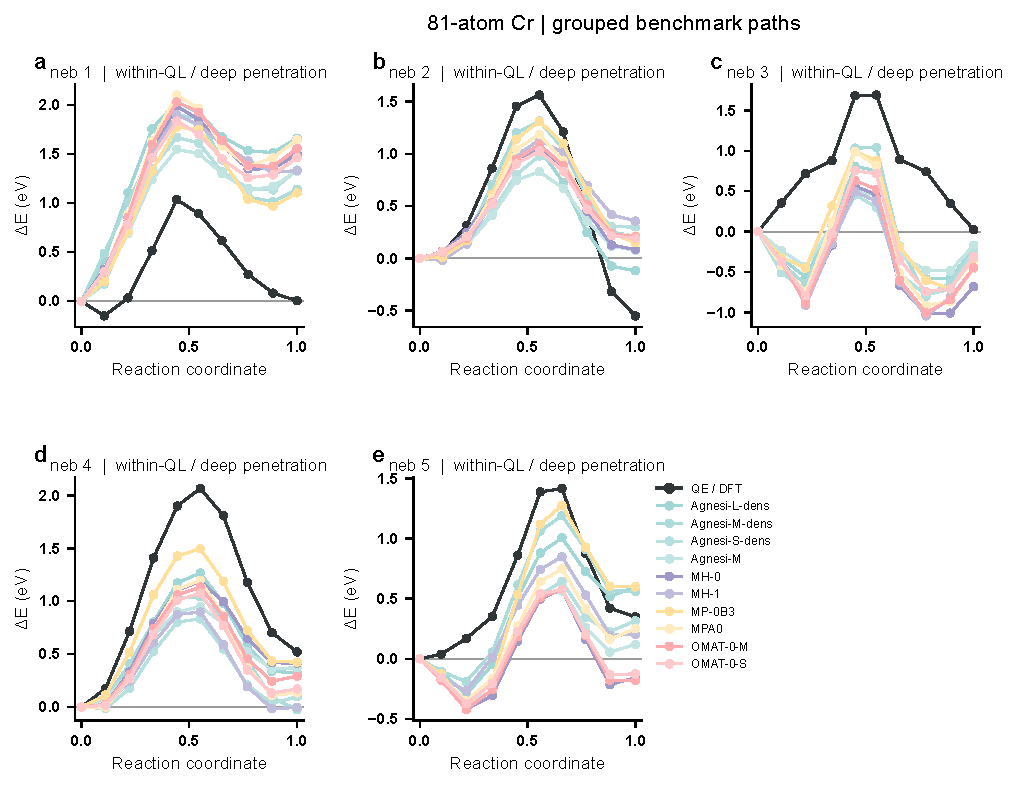
\includegraphics[width=\linewidth,height=0.42\textheight,keepaspectratio]{figure_pages/assets/fig_054.pdf}
\caption{Neb pathway, barrier, topology, or self-consistency diagnostics. This page shows the candidate output ``Figure cr81 grouped all foundation profiles'' within the audited TASK3-NEB family. The panel identity, source scope, and current status are retained in the accompanying evidence matrix.}
\label{fig:candidate_054}
\end{figure}
\textbf{Results text draft.} The panels distinguish fixed-path scoring, self-consistent MLFF-NEB behavior, endpoint/path topology checks, and DFT convergence status. These operators answer different questions and are kept separate in the text.
\textbf{Discussion and boundary.} A model-reported self-relaxed barrier must not be presented as the fixed-path DFT error, and a provisional or unconverged DFT path must not be promoted to a final reference barrier.
\textbf{Article placement.} Proposed article location: Results or SI: path-family diagnostics.
\textbf{Reviewer linkage:} overall status PARTIAL.
\begin{itemize}[leftmargin=1.4em,noitemsep]
\item \textbf{REV-A1 (PARTIAL):} Reconcile Fig. 3d fixed-geometry DFT-path scoring with SI Fig. S3 self-consistent MLFF-NEB, including pathway identity and the DFT reference. \emph{Completed:} The fixed-path versus self-relaxed operator distinction and the narrower model-reported-barrier wording are integrated. \emph{Still required:} Close the restartable QE path-1--4 convergence gate, preserve the final path/source metadata, and complete the SI Fig. S3 endpoint/checkpoint/optimizer/source audit before calling the quantitative reference final.
\end{itemize}
\textbf{Evidence pointers.}
\begin{itemize}[leftmargin=1.4em,noitemsep]
\item Data/processed: \begingroup\scriptsize\url{main/analysis/task3_endpoint_only_neb/exploratory_energy_audit/cr_61_81_three_class_20261003/61_atom_geometry_classification.csv}\endgroup
\item Data/processed: \begingroup\scriptsize\url{main/analysis/task3_endpoint_only_neb/exploratory_energy_audit/cr_61_81_three_class_20261003/61_atom_geometry_classification.json}\endgroup
\item Caption/text source: \begingroup\scriptsize\url{main/analysis/task3_endpoint_only_neb/exploratory_energy_audit/cr_61_81_three_class_20261003/Cr61_Cr81_foundation_comparison_report.md}\endgroup
\item Caption/text source: \begingroup\scriptsize\url{main/analysis/task3_endpoint_only_neb/exploratory_energy_audit/cr_61_81_three_class_20261003/Cr61_Cr81_publication_acceptance_matrix.tex}\endgroup
\end{itemize}
\statusline{\textbf{Audit gap / next action:} Many per-path exports have no co-located generator; use the parent renderer and record the exact input tables}
\vfill
\clearpage
\section{FIG-055 --- Figure cr81 in gap diffusion foundation profile}
\label{figpage:fig-055}
\textbf{Group:} TASK3-NEB\quad \textbf{Evidence chain:} partial\quad \textbf{Status:} exploratory;publication;audit
\begin{figure}[H]
\centering
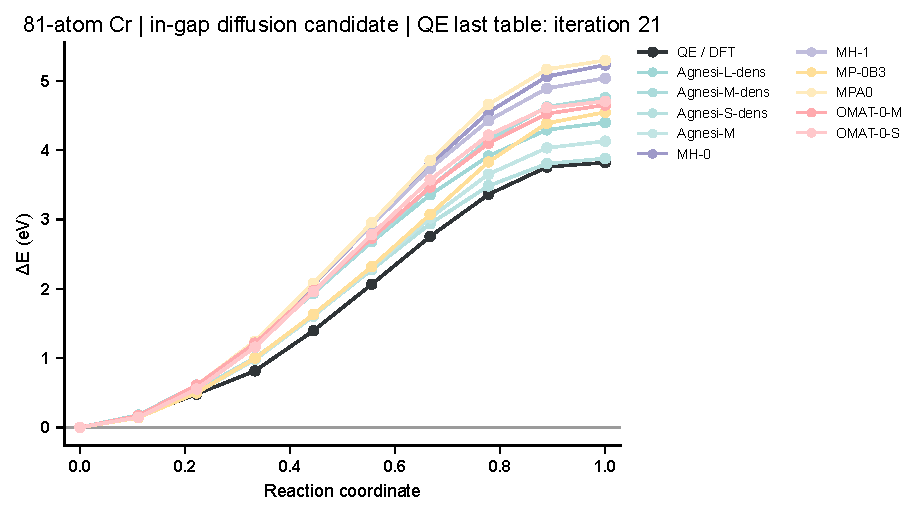
\includegraphics[width=\linewidth,height=0.42\textheight,keepaspectratio]{figure_pages/assets/fig_055.pdf}
\caption{Neb pathway, barrier, topology, or self-consistency diagnostics. This page shows the candidate output ``Figure cr81 in gap diffusion foundation profile'' within the audited TASK3-NEB family. The panel identity, source scope, and current status are retained in the accompanying evidence matrix.}
\label{fig:candidate_055}
\end{figure}
\textbf{Results text draft.} The panels distinguish fixed-path scoring, self-consistent MLFF-NEB behavior, endpoint/path topology checks, and DFT convergence status. These operators answer different questions and are kept separate in the text.
\textbf{Discussion and boundary.} A model-reported self-relaxed barrier must not be presented as the fixed-path DFT error, and a provisional or unconverged DFT path must not be promoted to a final reference barrier.
\textbf{Article placement.} Proposed article location: Results or SI: path-family diagnostics.
\textbf{Reviewer linkage:} overall status PARTIAL.
\begin{itemize}[leftmargin=1.4em,noitemsep]
\item \textbf{REV-A1 (PARTIAL):} Reconcile Fig. 3d fixed-geometry DFT-path scoring with SI Fig. S3 self-consistent MLFF-NEB, including pathway identity and the DFT reference. \emph{Completed:} The fixed-path versus self-relaxed operator distinction and the narrower model-reported-barrier wording are integrated. \emph{Still required:} Close the restartable QE path-1--4 convergence gate, preserve the final path/source metadata, and complete the SI Fig. S3 endpoint/checkpoint/optimizer/source audit before calling the quantitative reference final.
\end{itemize}
\textbf{Evidence pointers.}
\begin{itemize}[leftmargin=1.4em,noitemsep]
\item Data/processed: \begingroup\scriptsize\url{main/analysis/task3_endpoint_only_neb/exploratory_energy_audit/cr_61_81_three_class_20261003/61_atom_geometry_classification.csv}\endgroup
\item Data/processed: \begingroup\scriptsize\url{main/analysis/task3_endpoint_only_neb/exploratory_energy_audit/cr_61_81_three_class_20261003/61_atom_geometry_classification.json}\endgroup
\item Caption/text source: \begingroup\scriptsize\url{main/analysis/task3_endpoint_only_neb/exploratory_energy_audit/cr_61_81_three_class_20261003/Cr61_Cr81_foundation_comparison_report.md}\endgroup
\item Caption/text source: \begingroup\scriptsize\url{main/analysis/task3_endpoint_only_neb/exploratory_energy_audit/cr_61_81_three_class_20261003/Cr61_Cr81_publication_acceptance_matrix.tex}\endgroup
\end{itemize}
\statusline{\textbf{Audit gap / next action:} Many per-path exports have no co-located generator; use the parent renderer and record the exact input tables}
\vfill
\clearpage
\section{FIG-056 --- Figure diagnostic framework overview}
\label{figpage:fig-056}
\textbf{Group:} TASK3-NEB\quad \textbf{Evidence chain:} partial\quad \textbf{Status:} exploratory;audit
\begin{figure}[H]
\centering
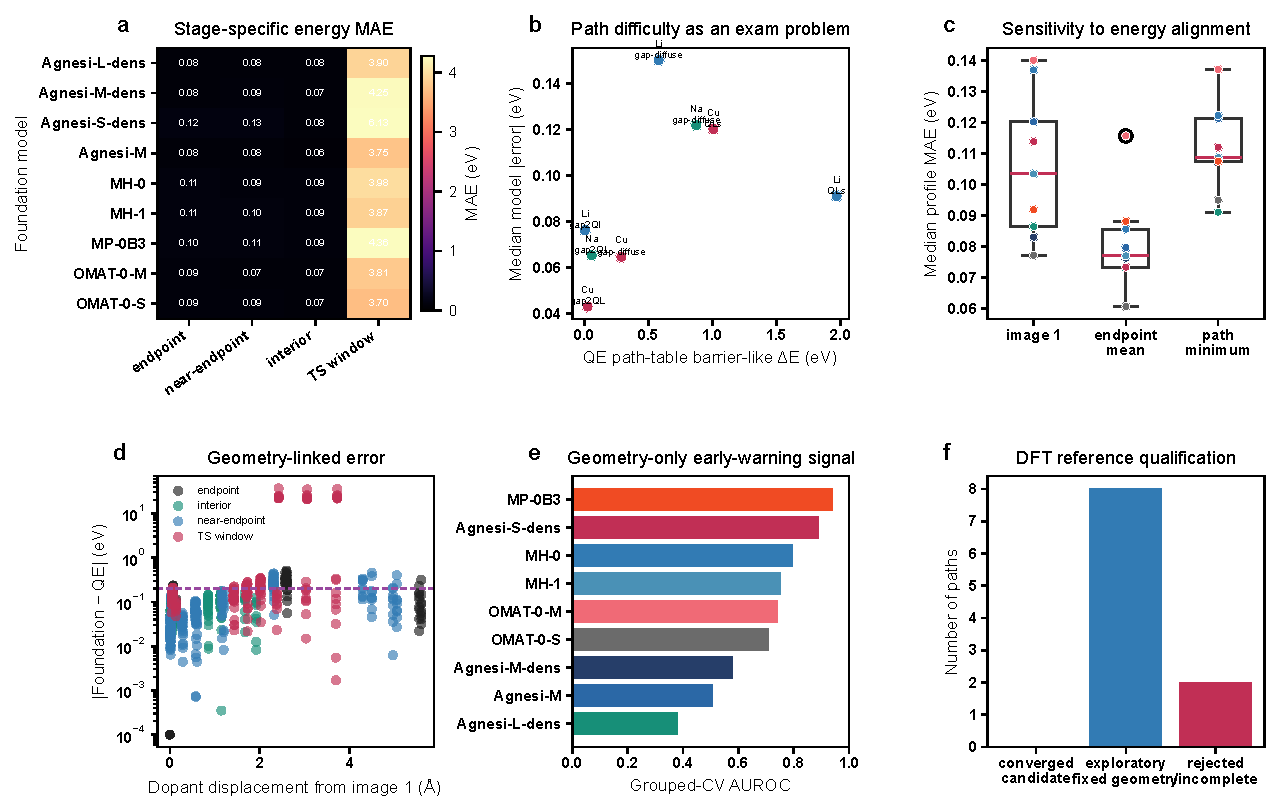
\includegraphics[width=\linewidth,height=0.42\textheight,keepaspectratio]{figure_pages/assets/fig_056.pdf}
\caption{Neb pathway, barrier, topology, or self-consistency diagnostics. This page shows the candidate output ``Figure diagnostic framework overview'' within the audited TASK3-NEB family. The panel identity, source scope, and current status are retained in the accompanying evidence matrix.}
\label{fig:candidate_056}
\end{figure}
\textbf{Results text draft.} The panels distinguish fixed-path scoring, self-consistent MLFF-NEB behavior, endpoint/path topology checks, and DFT convergence status. These operators answer different questions and are kept separate in the text.
\textbf{Discussion and boundary.} A model-reported self-relaxed barrier must not be presented as the fixed-path DFT error, and a provisional or unconverged DFT path must not be promoted to a final reference barrier.
\textbf{Article placement.} Proposed article location: Results or SI: path-family diagnostics.
\textbf{Reviewer linkage:} overall status PARTIAL.
\begin{itemize}[leftmargin=1.4em,noitemsep]
\item \textbf{REV-A1 (PARTIAL):} Reconcile Fig. 3d fixed-geometry DFT-path scoring with SI Fig. S3 self-consistent MLFF-NEB, including pathway identity and the DFT reference. \emph{Completed:} The fixed-path versus self-relaxed operator distinction and the narrower model-reported-barrier wording are integrated. \emph{Still required:} Close the restartable QE path-1--4 convergence gate, preserve the final path/source metadata, and complete the SI Fig. S3 endpoint/checkpoint/optimizer/source audit before calling the quantitative reference final.
\end{itemize}
\textbf{Evidence pointers.}
\begin{itemize}[leftmargin=1.4em,noitemsep]
\item Data/processed: \begingroup\scriptsize\url{main/analysis/task3_endpoint_only_neb/exploratory_energy_audit/audit_summary.json}\endgroup
\item Data/processed: \begingroup\scriptsize\url{main/analysis/task3_endpoint_only_neb/exploratory_energy_audit/diagnostic_framework/alignment_profile_errors.csv}\endgroup
\item Plot/processing script: \begingroup\scriptsize\url{main/analysis/task3_endpoint_only_neb/exploratory_energy_audit/plot_paper_figures.py}\endgroup
\item Caption/text source: \begingroup\scriptsize\url{main/analysis/task3_endpoint_only_neb/exploratory_energy_audit/ACCEPTANCE_MATRIX.md}\endgroup
\item Caption/text source: \begingroup\scriptsize\url{main/analysis/task3_endpoint_only_neb/exploratory_energy_audit/EXPLORATORY_REPORT.md}\endgroup
\end{itemize}
\statusline{\textbf{Audit gap / next action:} Many per-path exports have no co-located generator; use the parent renderer and record the exact input tables}
\vfill
\clearpage
\section{FIG-057 --- Figure1 task type matrix}
\label{figpage:fig-057}
\textbf{Group:} TASK3-NEB\quad \textbf{Evidence chain:} partial\quad \textbf{Status:} exploratory;audit
\begin{figure}[H]
\centering
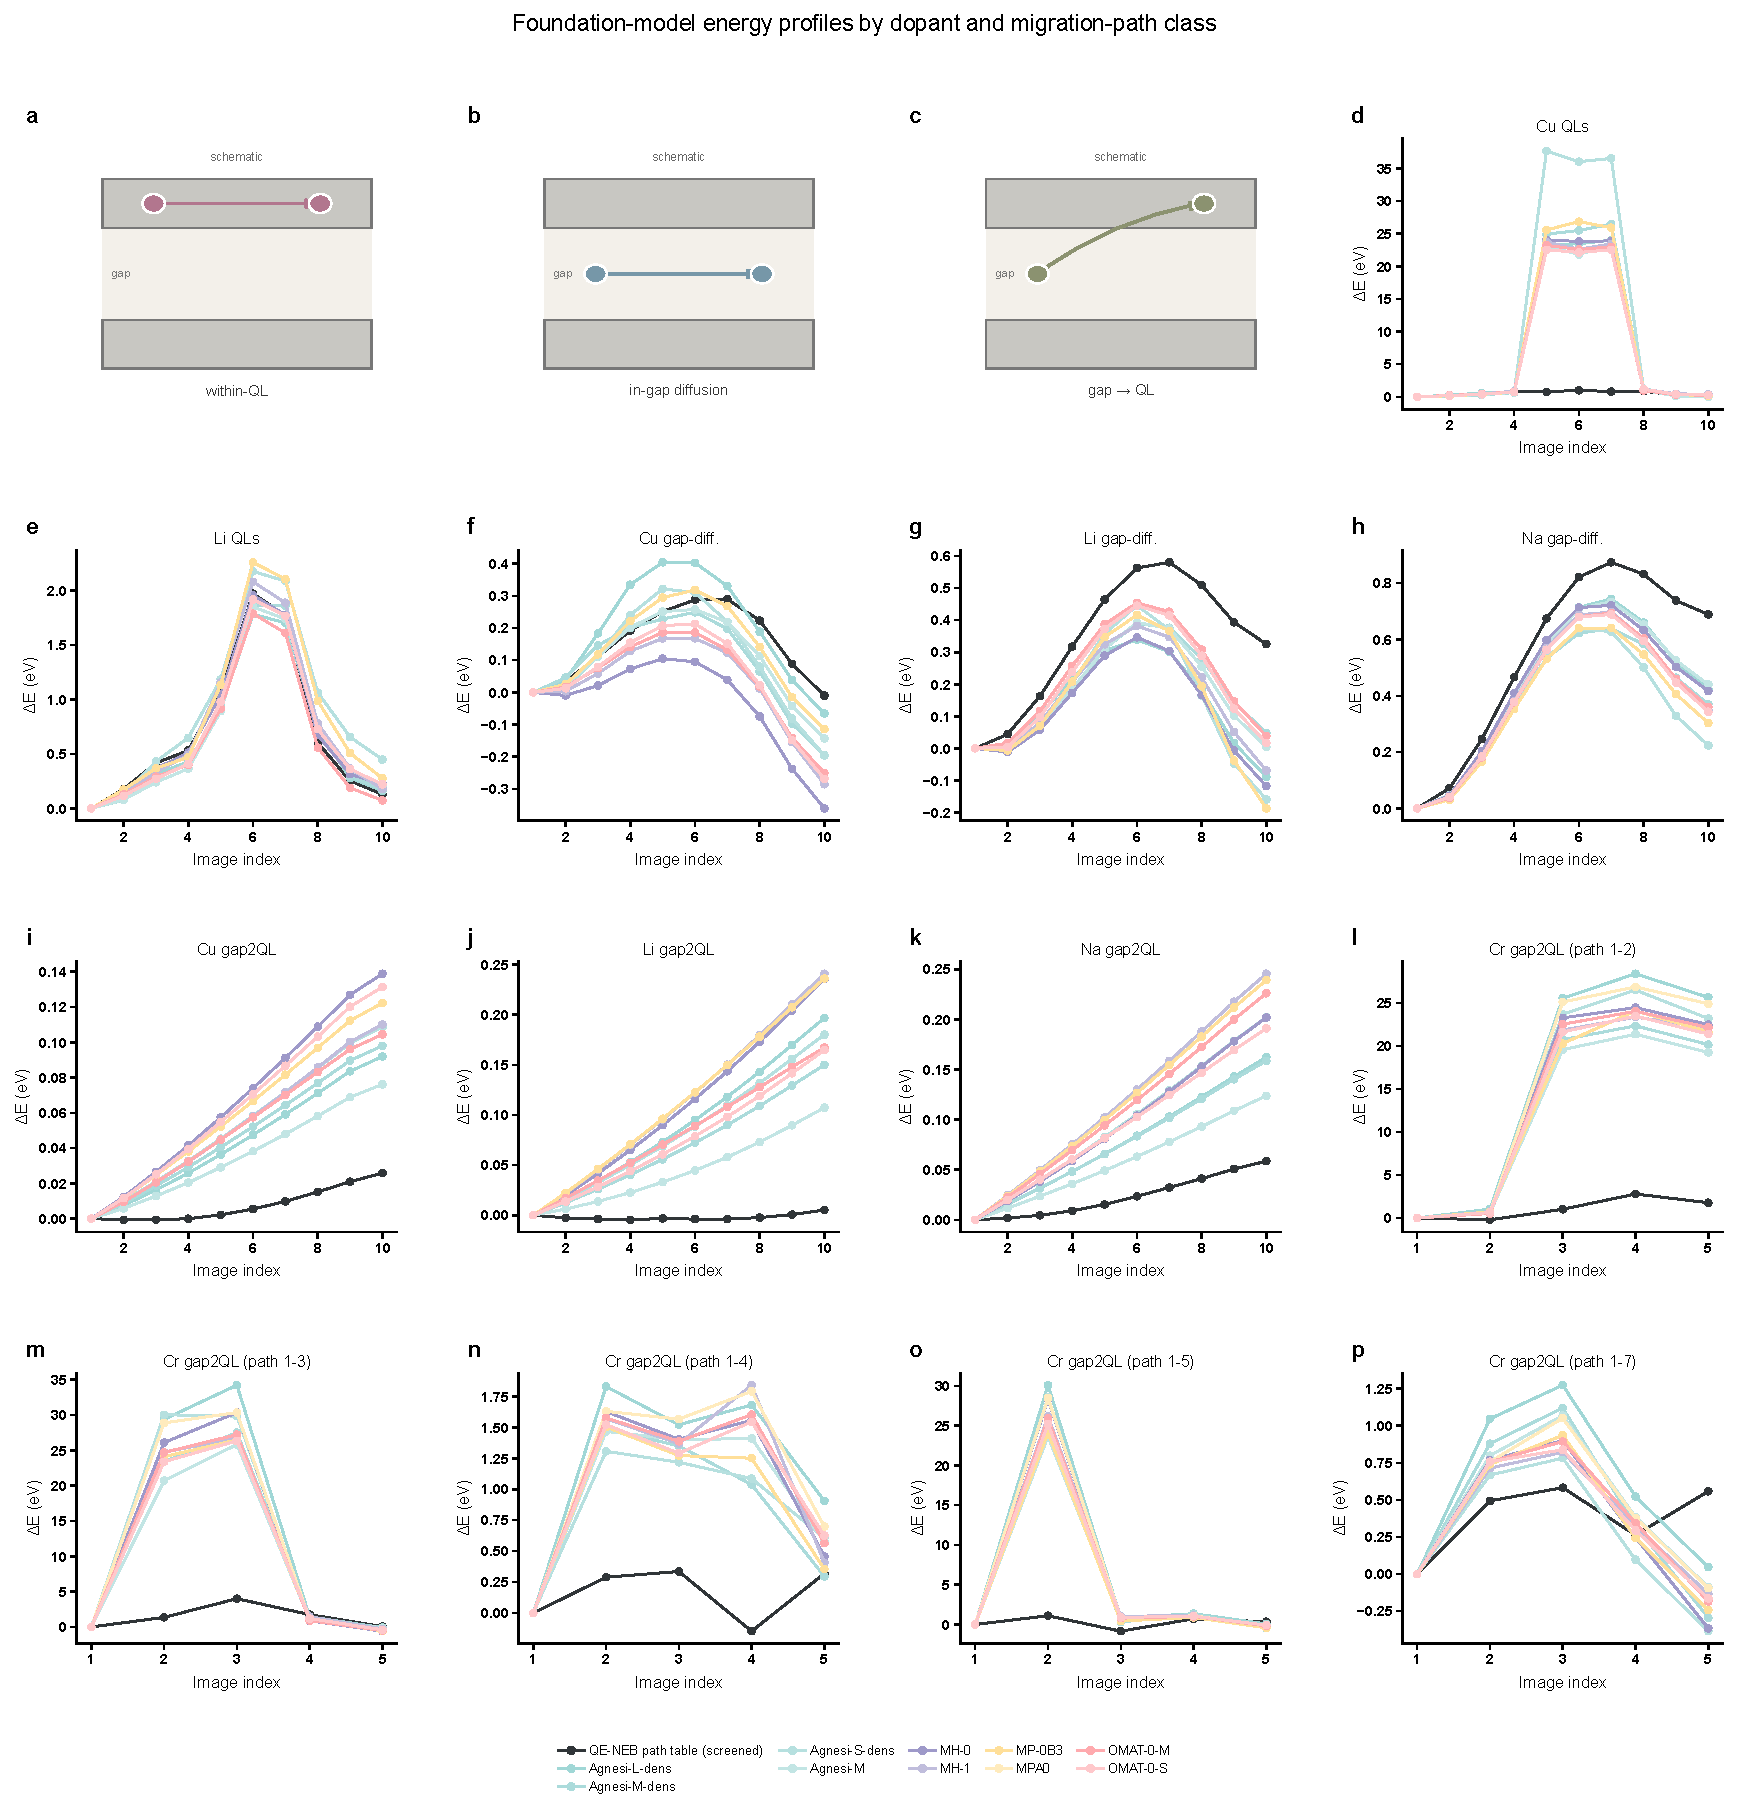
\includegraphics[width=\linewidth,height=0.42\textheight,keepaspectratio]{figure_pages/assets/fig_057.pdf}
\caption{Neb pathway, barrier, topology, or self-consistency diagnostics. This page shows the candidate output ``Figure1 task type matrix'' within the audited TASK3-NEB family. The panel identity, source scope, and current status are retained in the accompanying evidence matrix.}
\label{fig:candidate_057}
\end{figure}
\textbf{Results text draft.} The panels distinguish fixed-path scoring, self-consistent MLFF-NEB behavior, endpoint/path topology checks, and DFT convergence status. These operators answer different questions and are kept separate in the text.
\textbf{Discussion and boundary.} A model-reported self-relaxed barrier must not be presented as the fixed-path DFT error, and a provisional or unconverged DFT path must not be promoted to a final reference barrier.
\textbf{Article placement.} Proposed article location: Results or SI: path-family diagnostics.
\textbf{Reviewer linkage:} overall status PARTIAL.
\begin{itemize}[leftmargin=1.4em,noitemsep]
\item \textbf{REV-A1 (PARTIAL):} Reconcile Fig. 3d fixed-geometry DFT-path scoring with SI Fig. S3 self-consistent MLFF-NEB, including pathway identity and the DFT reference. \emph{Completed:} The fixed-path versus self-relaxed operator distinction and the narrower model-reported-barrier wording are integrated. \emph{Still required:} Close the restartable QE path-1--4 convergence gate, preserve the final path/source metadata, and complete the SI Fig. S3 endpoint/checkpoint/optimizer/source audit before calling the quantitative reference final.
\end{itemize}
\textbf{Evidence pointers.}
\begin{itemize}[leftmargin=1.4em,noitemsep]
\item Data/processed: \begingroup\scriptsize\url{main/analysis/task3_endpoint_only_neb/exploratory_energy_audit/audit_summary.json}\endgroup
\item Data/processed: \begingroup\scriptsize\url{main/analysis/task3_endpoint_only_neb/exploratory_energy_audit/figure1_task_type_matrix/cr_foundation_path_barriers.csv}\endgroup
\item Plot/processing script: \begingroup\scriptsize\url{main/analysis/task3_endpoint_only_neb/exploratory_energy_audit/plot_paper_figures.py}\endgroup
\item Caption/text source: \begingroup\scriptsize\url{main/analysis/task3_endpoint_only_neb/exploratory_energy_audit/ACCEPTANCE_MATRIX.md}\endgroup
\item Caption/text source: \begingroup\scriptsize\url{main/analysis/task3_endpoint_only_neb/exploratory_energy_audit/EXPLORATORY_REPORT.md}\endgroup
\end{itemize}
\statusline{\textbf{Audit gap / next action:} Many per-path exports have no co-located generator; use the parent renderer and record the exact input tables}
\vfill
\clearpage
\section{FIG-058 --- Figure all foundation model path profiles}
\label{figpage:fig-058}
\textbf{Group:} TASK3-NEB\quad \textbf{Evidence chain:} partial\quad \textbf{Status:} exploratory;audit;comparison
\begin{figure}[H]
\centering
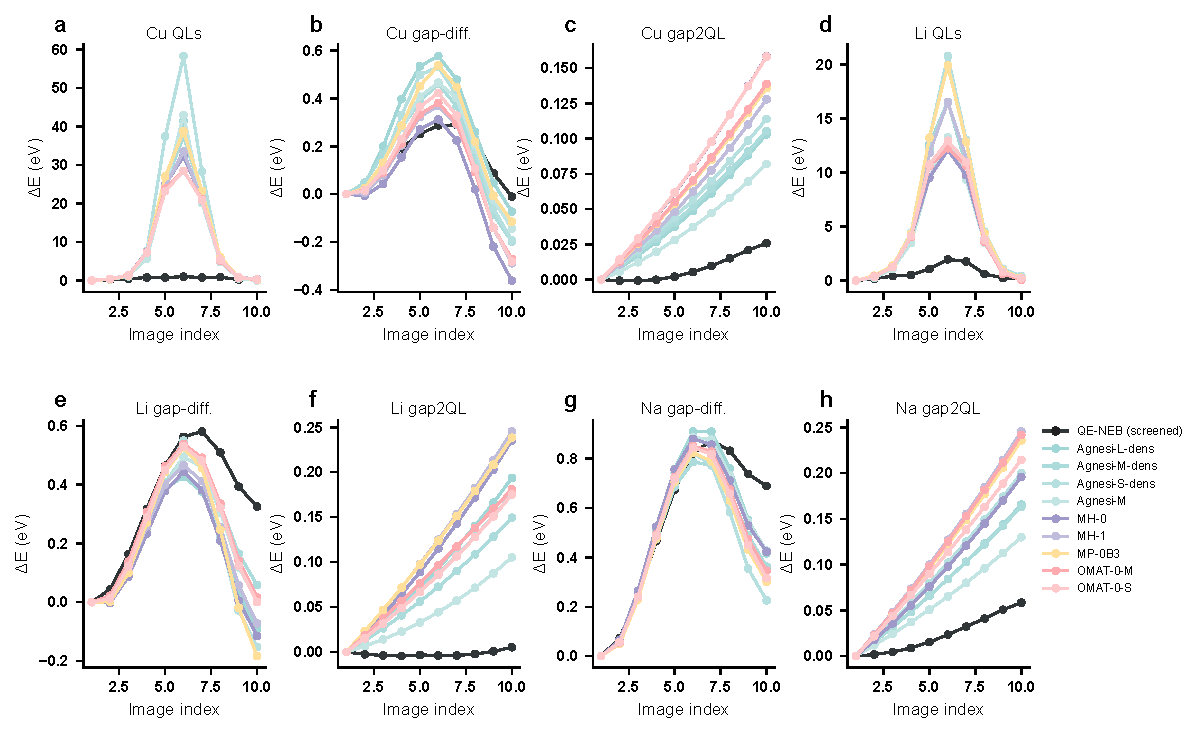
\includegraphics[width=\linewidth,height=0.42\textheight,keepaspectratio]{figure_pages/assets/fig_058.pdf}
\caption{Neb pathway, barrier, topology, or self-consistency diagnostics. This page shows the candidate output ``Figure all foundation model path profiles'' within the audited TASK3-NEB family. The panel identity, source scope, and current status are retained in the accompanying evidence matrix.}
\label{fig:candidate_058}
\end{figure}
\textbf{Results text draft.} The panels distinguish fixed-path scoring, self-consistent MLFF-NEB behavior, endpoint/path topology checks, and DFT convergence status. These operators answer different questions and are kept separate in the text.
\textbf{Discussion and boundary.} A model-reported self-relaxed barrier must not be presented as the fixed-path DFT error, and a provisional or unconverged DFT path must not be promoted to a final reference barrier.
\textbf{Article placement.} Proposed article location: Results or SI: path-family diagnostics.
\textbf{Reviewer linkage:} overall status PARTIAL.
\begin{itemize}[leftmargin=1.4em,noitemsep]
\item \textbf{REV-A1 (PARTIAL):} Reconcile Fig. 3d fixed-geometry DFT-path scoring with SI Fig. S3 self-consistent MLFF-NEB, including pathway identity and the DFT reference. \emph{Completed:} The fixed-path versus self-relaxed operator distinction and the narrower model-reported-barrier wording are integrated. \emph{Still required:} Close the restartable QE path-1--4 convergence gate, preserve the final path/source metadata, and complete the SI Fig. S3 endpoint/checkpoint/optimizer/source audit before calling the quantitative reference final.
\end{itemize}
\textbf{Evidence pointers.}
\begin{itemize}[leftmargin=1.4em,noitemsep]
\item Data/processed: \begingroup\scriptsize\url{main/analysis/task3_endpoint_only_neb/exploratory_energy_audit/audit_summary.json}\endgroup
\item Data/processed: \begingroup\scriptsize\url{main/analysis/task3_endpoint_only_neb/exploratory_energy_audit/full_foundation_models/all_foundation_model_image_profiles.csv}\endgroup
\item Plot/processing script: \begingroup\scriptsize\url{main/analysis/task3_endpoint_only_neb/exploratory_energy_audit/plot_paper_figures.py}\endgroup
\item Caption/text source: \begingroup\scriptsize\url{main/analysis/task3_endpoint_only_neb/exploratory_energy_audit/ACCEPTANCE_MATRIX.md}\endgroup
\item Caption/text source: \begingroup\scriptsize\url{main/analysis/task3_endpoint_only_neb/exploratory_energy_audit/EXPLORATORY_REPORT.md}\endgroup
\end{itemize}
\statusline{\textbf{Audit gap / next action:} Many per-path exports have no co-located generator; use the parent renderer and record the exact input tables}
\vfill
\clearpage
\section{FIG-059 --- Figure all foundation model spread}
\label{figpage:fig-059}
\textbf{Group:} TASK3-NEB\quad \textbf{Evidence chain:} partial\quad \textbf{Status:} exploratory;audit
\begin{figure}[H]
\centering
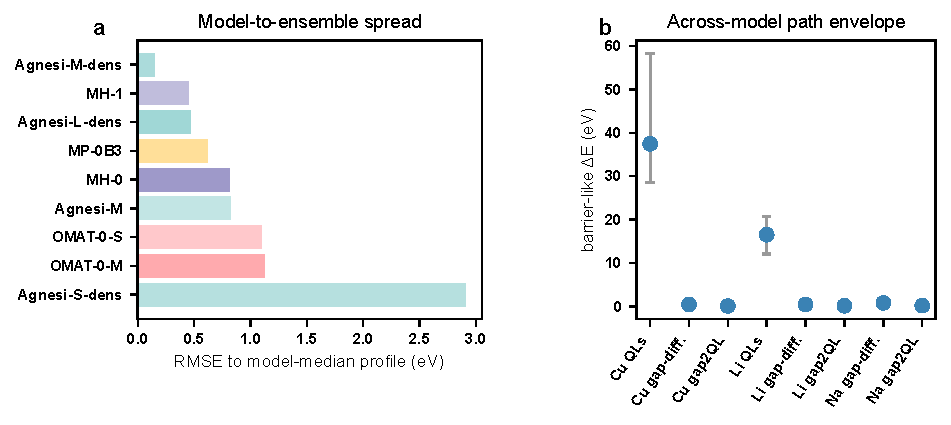
\includegraphics[width=\linewidth,height=0.42\textheight,keepaspectratio]{figure_pages/assets/fig_059.pdf}
\caption{Neb pathway, barrier, topology, or self-consistency diagnostics. This page shows the candidate output ``Figure all foundation model spread'' within the audited TASK3-NEB family. The panel identity, source scope, and current status are retained in the accompanying evidence matrix.}
\label{fig:candidate_059}
\end{figure}
\textbf{Results text draft.} The panels distinguish fixed-path scoring, self-consistent MLFF-NEB behavior, endpoint/path topology checks, and DFT convergence status. These operators answer different questions and are kept separate in the text.
\textbf{Discussion and boundary.} A model-reported self-relaxed barrier must not be presented as the fixed-path DFT error, and a provisional or unconverged DFT path must not be promoted to a final reference barrier.
\textbf{Article placement.} Proposed article location: Results or SI: path-family diagnostics.
\textbf{Reviewer linkage:} overall status PARTIAL.
\begin{itemize}[leftmargin=1.4em,noitemsep]
\item \textbf{REV-A1 (PARTIAL):} Reconcile Fig. 3d fixed-geometry DFT-path scoring with SI Fig. S3 self-consistent MLFF-NEB, including pathway identity and the DFT reference. \emph{Completed:} The fixed-path versus self-relaxed operator distinction and the narrower model-reported-barrier wording are integrated. \emph{Still required:} Close the restartable QE path-1--4 convergence gate, preserve the final path/source metadata, and complete the SI Fig. S3 endpoint/checkpoint/optimizer/source audit before calling the quantitative reference final.
\end{itemize}
\textbf{Evidence pointers.}
\begin{itemize}[leftmargin=1.4em,noitemsep]
\item Data/processed: \begingroup\scriptsize\url{main/analysis/task3_endpoint_only_neb/exploratory_energy_audit/audit_summary.json}\endgroup
\item Data/processed: \begingroup\scriptsize\url{main/analysis/task3_endpoint_only_neb/exploratory_energy_audit/full_foundation_models/all_foundation_model_image_profiles.csv}\endgroup
\item Plot/processing script: \begingroup\scriptsize\url{main/analysis/task3_endpoint_only_neb/exploratory_energy_audit/plot_paper_figures.py}\endgroup
\item Caption/text source: \begingroup\scriptsize\url{main/analysis/task3_endpoint_only_neb/exploratory_energy_audit/ACCEPTANCE_MATRIX.md}\endgroup
\item Caption/text source: \begingroup\scriptsize\url{main/analysis/task3_endpoint_only_neb/exploratory_energy_audit/EXPLORATORY_REPORT.md}\endgroup
\end{itemize}
\statusline{\textbf{Audit gap / next action:} Many per-path exports have no co-located generator; use the parent renderer and record the exact input tables}
\vfill
\clearpage
\section{FIG-060 --- Figure neb residual audit}
\label{figpage:fig-060}
\textbf{Group:} TASK3-NEB\quad \textbf{Evidence chain:} partial\quad \textbf{Status:} exploratory;audit
\begin{figure}[H]
\centering
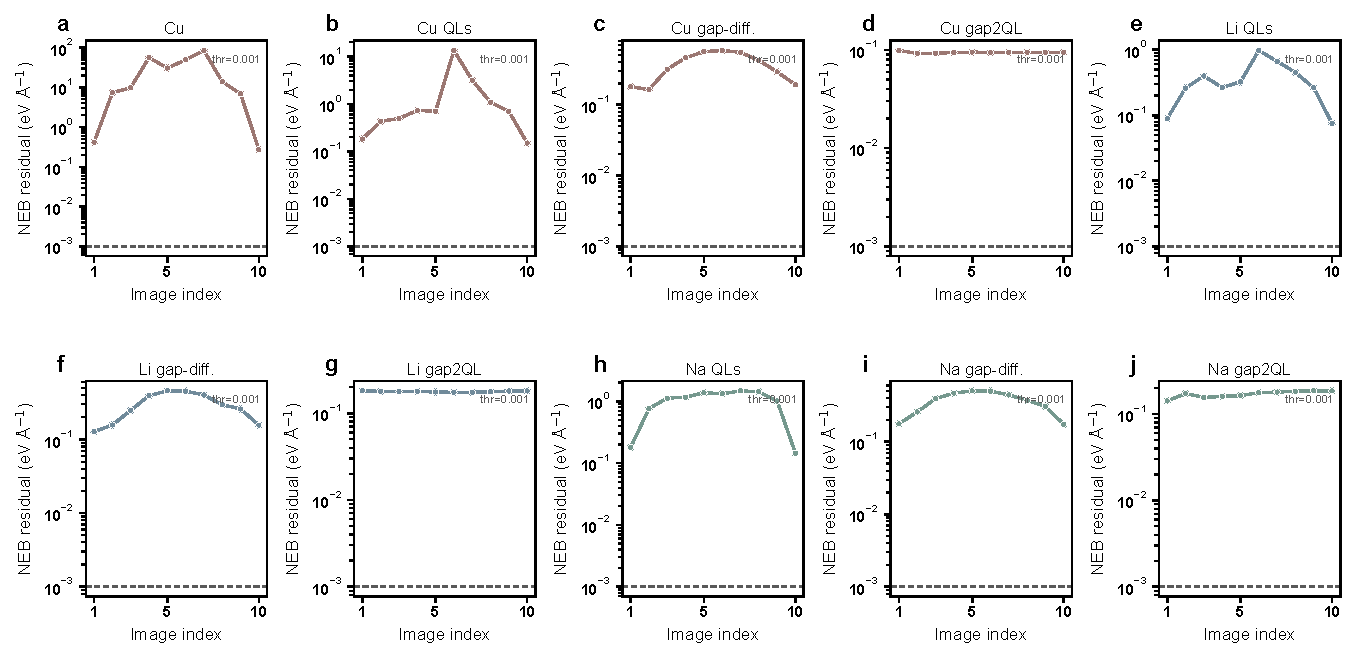
\includegraphics[width=\linewidth,height=0.42\textheight,keepaspectratio]{figure_pages/assets/fig_060.pdf}
\caption{Neb pathway, barrier, topology, or self-consistency diagnostics. This page shows the candidate output ``Figure neb residual audit'' within the audited TASK3-NEB family. The panel identity, source scope, and current status are retained in the accompanying evidence matrix.}
\label{fig:candidate_060}
\end{figure}
\textbf{Results text draft.} The panels distinguish fixed-path scoring, self-consistent MLFF-NEB behavior, endpoint/path topology checks, and DFT convergence status. These operators answer different questions and are kept separate in the text.
\textbf{Discussion and boundary.} A model-reported self-relaxed barrier must not be presented as the fixed-path DFT error, and a provisional or unconverged DFT path must not be promoted to a final reference barrier.
\textbf{Article placement.} Proposed article location: Results or SI: path-family diagnostics.
\textbf{Reviewer linkage:} overall status PARTIAL.
\begin{itemize}[leftmargin=1.4em,noitemsep]
\item \textbf{REV-A1 (PARTIAL):} Reconcile Fig. 3d fixed-geometry DFT-path scoring with SI Fig. S3 self-consistent MLFF-NEB, including pathway identity and the DFT reference. \emph{Completed:} The fixed-path versus self-relaxed operator distinction and the narrower model-reported-barrier wording are integrated. \emph{Still required:} Close the restartable QE path-1--4 convergence gate, preserve the final path/source metadata, and complete the SI Fig. S3 endpoint/checkpoint/optimizer/source audit before calling the quantitative reference final.
\end{itemize}
\textbf{Evidence pointers.}
\begin{itemize}[leftmargin=1.4em,noitemsep]
\item Data/processed: \begingroup\scriptsize\url{main/analysis/task3_endpoint_only_neb/exploratory_energy_audit/audit_summary.json}\endgroup
\item Data/processed: \begingroup\scriptsize\url{main/analysis/task3_endpoint_only_neb/exploratory_energy_audit/neb_convergence_audit/qe_neb_image_residual_audit.csv}\endgroup
\item Plot/processing script: \begingroup\scriptsize\url{main/analysis/task3_endpoint_only_neb/exploratory_energy_audit/plot_paper_figures.py}\endgroup
\item Caption/text source: \begingroup\scriptsize\url{main/analysis/task3_endpoint_only_neb/exploratory_energy_audit/ACCEPTANCE_MATRIX.md}\endgroup
\item Caption/text source: \begingroup\scriptsize\url{main/analysis/task3_endpoint_only_neb/exploratory_energy_audit/EXPLORATORY_REPORT.md}\endgroup
\end{itemize}
\statusline{\textbf{Audit gap / next action:} Many per-path exports have no co-located generator; use the parent renderer and record the exact input tables}
\vfill
\clearpage
\section{FIG-061 --- Figure 1 stability parity perturbation}
\label{figpage:fig-061}
\textbf{Group:} TASK3-NEB\quad \textbf{Evidence chain:} partial\quad \textbf{Status:} exploratory;audit;comparison
\begin{figure}[H]
\centering
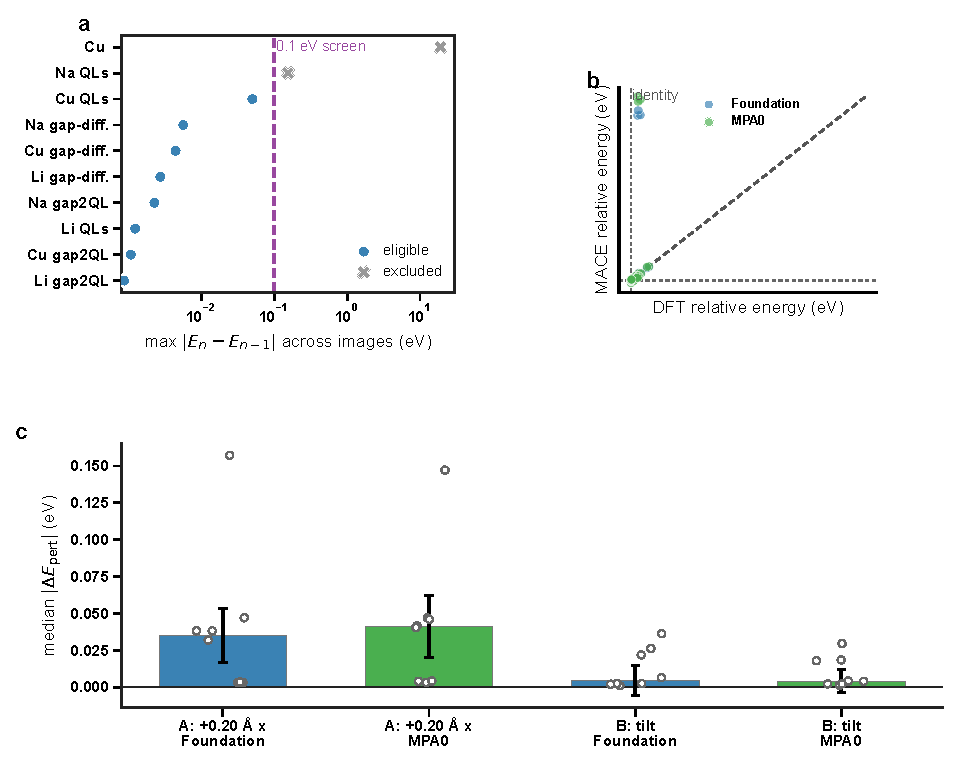
\includegraphics[width=\linewidth,height=0.42\textheight,keepaspectratio]{figure_pages/assets/fig_061.pdf}
\caption{Neb pathway, barrier, topology, or self-consistency diagnostics. This page shows the candidate output ``Figure 1 stability parity perturbation'' within the audited TASK3-NEB family. The panel identity, source scope, and current status are retained in the accompanying evidence matrix.}
\label{fig:candidate_061}
\end{figure}
\textbf{Results text draft.} The panels distinguish fixed-path scoring, self-consistent MLFF-NEB behavior, endpoint/path topology checks, and DFT convergence status. These operators answer different questions and are kept separate in the text.
\textbf{Discussion and boundary.} A model-reported self-relaxed barrier must not be presented as the fixed-path DFT error, and a provisional or unconverged DFT path must not be promoted to a final reference barrier.
\textbf{Article placement.} Proposed article location: Results or SI: path-family diagnostics.
\textbf{Reviewer linkage:} overall status PARTIAL.
\begin{itemize}[leftmargin=1.4em,noitemsep]
\item \textbf{REV-A1 (PARTIAL):} Reconcile Fig. 3d fixed-geometry DFT-path scoring with SI Fig. S3 self-consistent MLFF-NEB, including pathway identity and the DFT reference. \emph{Completed:} The fixed-path versus self-relaxed operator distinction and the narrower model-reported-barrier wording are integrated. \emph{Still required:} Close the restartable QE path-1--4 convergence gate, preserve the final path/source metadata, and complete the SI Fig. S3 endpoint/checkpoint/optimizer/source audit before calling the quantitative reference final.
\end{itemize}
\textbf{Evidence pointers.}
\begin{itemize}[leftmargin=1.4em,noitemsep]
\item Data/processed: \begingroup\scriptsize\url{main/analysis/task3_endpoint_only_neb/exploratory_energy_audit/processed/analysis_manifest.json}\endgroup
\item Data/processed: \begingroup\scriptsize\url{main/analysis/task3_endpoint_only_neb/exploratory_energy_audit/processed/figures/table_1_model_summary.csv}\endgroup
\item Caption/text source: \begingroup\scriptsize\url{main/analysis/task3_endpoint_only_neb/exploratory_energy_audit/processed/figures/captions_and_discussion.md}\endgroup
\item Caption/text source: \begingroup\scriptsize\url{main/analysis/task3_endpoint_only_neb/exploratory_energy_audit/processed/figures/table_1_model_summary.tex}\endgroup
\end{itemize}
\statusline{\textbf{Audit gap / next action:} Many per-path exports have no co-located generator; use the parent renderer and record the exact input tables}
\vfill
\clearpage
\section{FIG-062 --- Figure 2 relative energy profiles}
\label{figpage:fig-062}
\textbf{Group:} TASK3-NEB\quad \textbf{Evidence chain:} partial\quad \textbf{Status:} exploratory;audit;comparison
\begin{figure}[H]
\centering
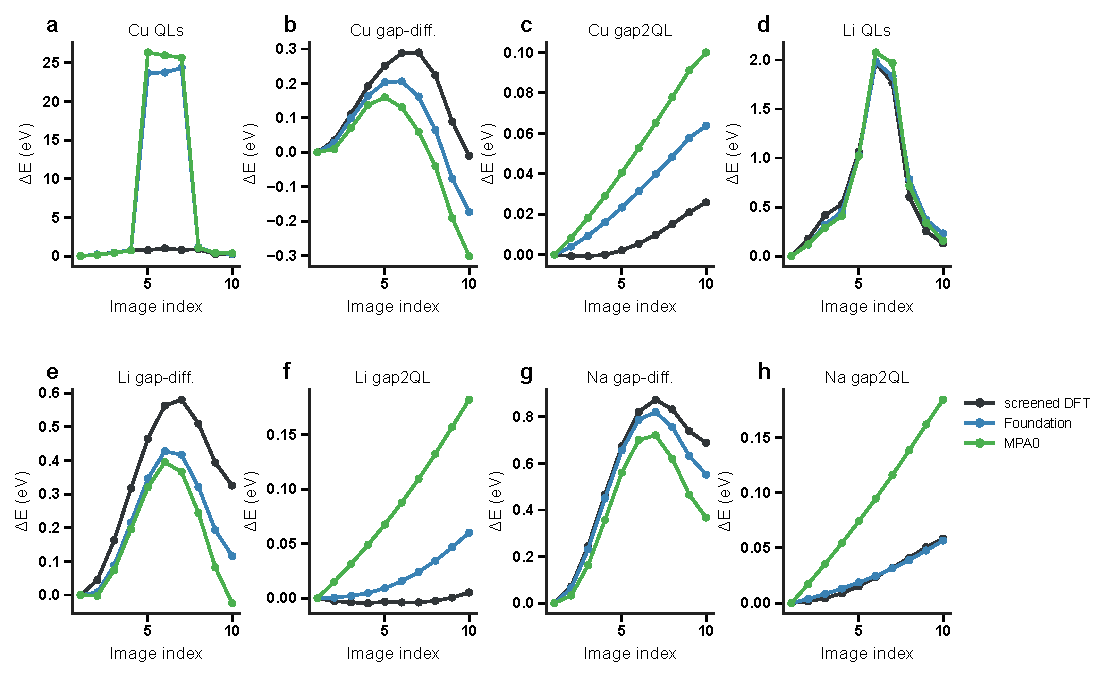
\includegraphics[width=\linewidth,height=0.42\textheight,keepaspectratio]{figure_pages/assets/fig_062.pdf}
\caption{Neb pathway, barrier, topology, or self-consistency diagnostics. This page shows the candidate output ``Figure 2 relative energy profiles'' within the audited TASK3-NEB family. The panel identity, source scope, and current status are retained in the accompanying evidence matrix.}
\label{fig:candidate_062}
\end{figure}
\textbf{Results text draft.} The panels distinguish fixed-path scoring, self-consistent MLFF-NEB behavior, endpoint/path topology checks, and DFT convergence status. These operators answer different questions and are kept separate in the text.
\textbf{Discussion and boundary.} A model-reported self-relaxed barrier must not be presented as the fixed-path DFT error, and a provisional or unconverged DFT path must not be promoted to a final reference barrier.
\textbf{Article placement.} Proposed article location: Results or SI: path-family diagnostics.
\textbf{Reviewer linkage:} overall status PARTIAL.
\begin{itemize}[leftmargin=1.4em,noitemsep]
\item \textbf{REV-A1 (PARTIAL):} Reconcile Fig. 3d fixed-geometry DFT-path scoring with SI Fig. S3 self-consistent MLFF-NEB, including pathway identity and the DFT reference. \emph{Completed:} The fixed-path versus self-relaxed operator distinction and the narrower model-reported-barrier wording are integrated. \emph{Still required:} Close the restartable QE path-1--4 convergence gate, preserve the final path/source metadata, and complete the SI Fig. S3 endpoint/checkpoint/optimizer/source audit before calling the quantitative reference final.
\end{itemize}
\textbf{Evidence pointers.}
\begin{itemize}[leftmargin=1.4em,noitemsep]
\item Data/processed: \begingroup\scriptsize\url{main/analysis/task3_endpoint_only_neb/exploratory_energy_audit/processed/analysis_manifest.json}\endgroup
\item Data/processed: \begingroup\scriptsize\url{main/analysis/task3_endpoint_only_neb/exploratory_energy_audit/processed/figures/table_1_model_summary.csv}\endgroup
\item Caption/text source: \begingroup\scriptsize\url{main/analysis/task3_endpoint_only_neb/exploratory_energy_audit/processed/figures/captions_and_discussion.md}\endgroup
\item Caption/text source: \begingroup\scriptsize\url{main/analysis/task3_endpoint_only_neb/exploratory_energy_audit/processed/figures/table_1_model_summary.tex}\endgroup
\end{itemize}
\statusline{\textbf{Audit gap / next action:} Many per-path exports have no co-located generator; use the parent renderer and record the exact input tables}
\vfill
\clearpage
\section{FIG-063 --- Figure structural stage diagnostics}
\label{figpage:fig-063}
\textbf{Group:} TASK3-NEB\quad \textbf{Evidence chain:} partial\quad \textbf{Status:} exploratory;audit
\begin{figure}[H]
\centering
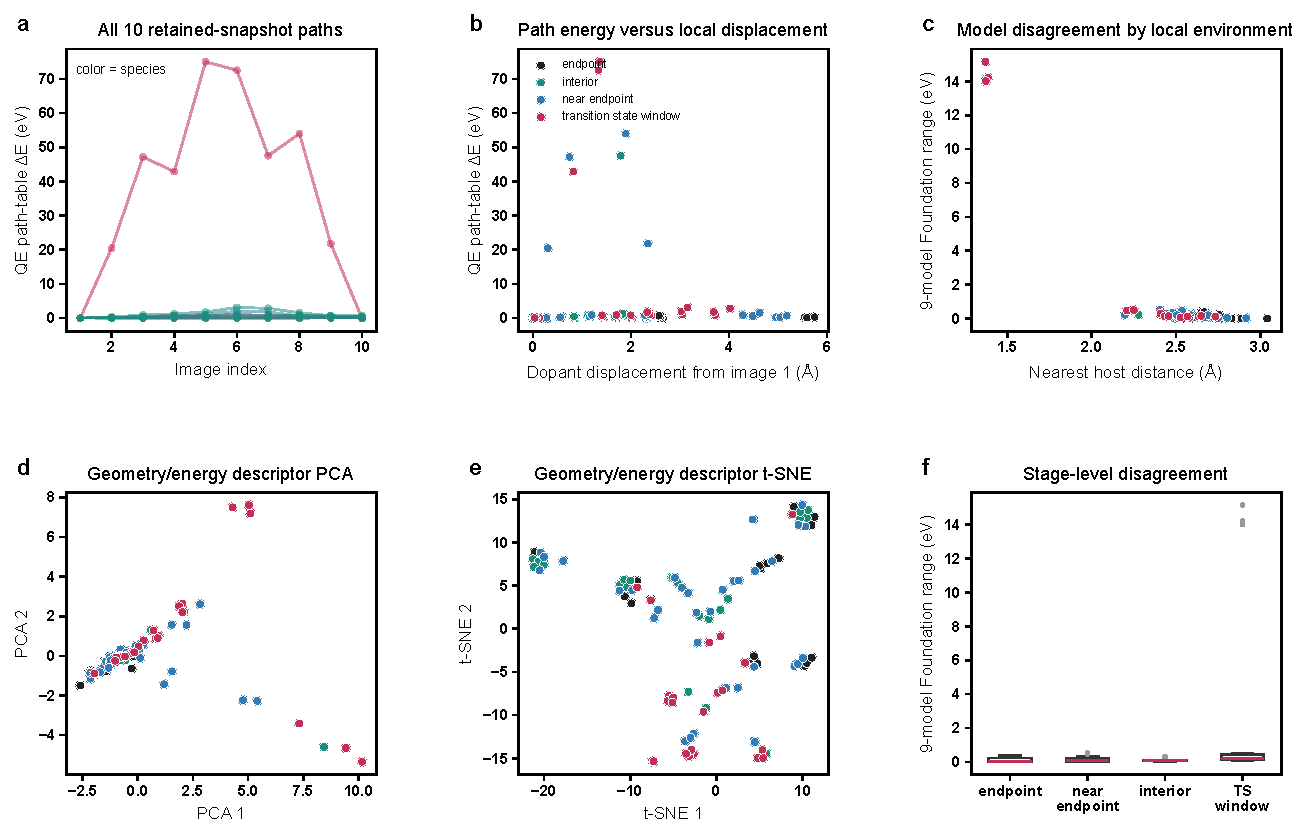
\includegraphics[width=\linewidth,height=0.42\textheight,keepaspectratio]{figure_pages/assets/fig_063.pdf}
\caption{Neb pathway, barrier, topology, or self-consistency diagnostics. This page shows the candidate output ``Figure structural stage diagnostics'' within the audited TASK3-NEB family. The panel identity, source scope, and current status are retained in the accompanying evidence matrix.}
\label{fig:candidate_063}
\end{figure}
\textbf{Results text draft.} The panels distinguish fixed-path scoring, self-consistent MLFF-NEB behavior, endpoint/path topology checks, and DFT convergence status. These operators answer different questions and are kept separate in the text.
\textbf{Discussion and boundary.} A model-reported self-relaxed barrier must not be presented as the fixed-path DFT error, and a provisional or unconverged DFT path must not be promoted to a final reference barrier.
\textbf{Article placement.} Proposed article location: Results or SI: path-family diagnostics.
\textbf{Reviewer linkage:} overall status PARTIAL.
\begin{itemize}[leftmargin=1.4em,noitemsep]
\item \textbf{REV-A1 (PARTIAL):} Reconcile Fig. 3d fixed-geometry DFT-path scoring with SI Fig. S3 self-consistent MLFF-NEB, including pathway identity and the DFT reference. \emph{Completed:} The fixed-path versus self-relaxed operator distinction and the narrower model-reported-barrier wording are integrated. \emph{Still required:} Close the restartable QE path-1--4 convergence gate, preserve the final path/source metadata, and complete the SI Fig. S3 endpoint/checkpoint/optimizer/source audit before calling the quantitative reference final.
\end{itemize}
\textbf{Evidence pointers.}
\begin{itemize}[leftmargin=1.4em,noitemsep]
\item Data/processed: \begingroup\scriptsize\url{main/analysis/task3_endpoint_only_neb/exploratory_energy_audit/audit_summary.json}\endgroup
\item Data/processed: \begingroup\scriptsize\url{main/analysis/task3_endpoint_only_neb/exploratory_energy_audit/scf_neb_image_energy_deltas.csv}\endgroup
\item Plot/processing script: \begingroup\scriptsize\url{main/analysis/task3_endpoint_only_neb/exploratory_energy_audit/plot_paper_figures.py}\endgroup
\item Caption/text source: \begingroup\scriptsize\url{main/analysis/task3_endpoint_only_neb/exploratory_energy_audit/ACCEPTANCE_MATRIX.md}\endgroup
\item Caption/text source: \begingroup\scriptsize\url{main/analysis/task3_endpoint_only_neb/exploratory_energy_audit/EXPLORATORY_REPORT.md}\endgroup
\end{itemize}
\statusline{\textbf{Audit gap / next action:} Many per-path exports have no co-located generator; use the parent renderer and record the exact input tables}
\vfill
\clearpage
\section{FIG-064 --- Fig from scratch failure}
\label{figpage:fig-064}
\textbf{Group:} MD-1NS-LEGACY\quad \textbf{Evidence chain:} partial\quad \textbf{Status:} publication
\begin{figure}[H]
\centering
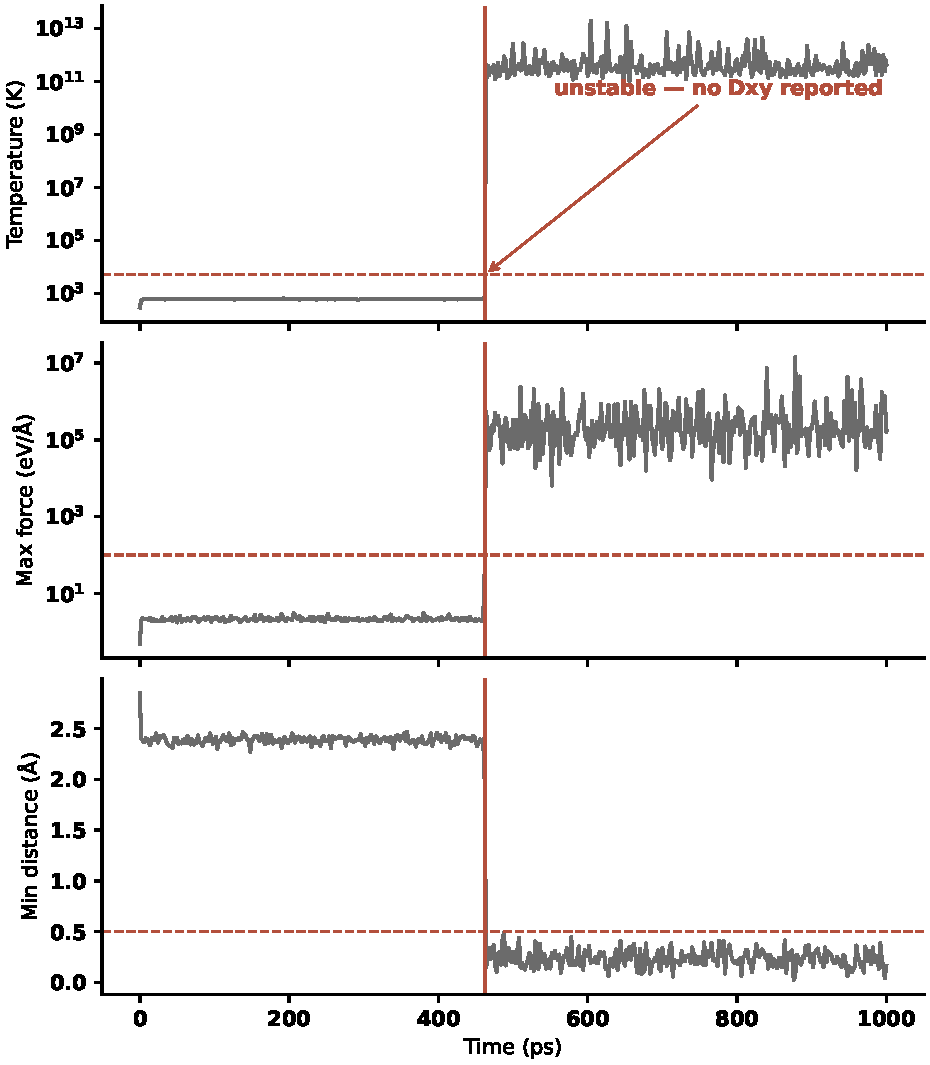
\includegraphics[width=\linewidth,height=0.42\textheight,keepaspectratio]{figure_pages/assets/fig_064.pdf}
\caption{Legacy one-nanosecond molecular-dynamics diagnostics retained for provenance comparison. This page shows the candidate output ``Fig from scratch failure'' within the audited MD-1NS-LEGACY family. The panel identity, source scope, and current status are retained in the accompanying evidence matrix.}
\label{fig:candidate_064}
\end{figure}
\textbf{Results text draft.} The figure records an earlier diagnostic view of the molecular-dynamics campaign and is useful for tracing how the analysis evolved. It is not automatically equivalent to the matched-protocol re-analysis.
\textbf{Discussion and boundary.} Use as historical or audit material only unless the local manifest confirms the current protocol, seeds, trajectory completeness, and acceptance gates.
\textbf{Article placement.} Proposed article location: SI transport or audit appendix only.
\textbf{Reviewer linkage:} overall status PENDING.
\begin{itemize}[leftmargin=1.4em,noitemsep]
\item \textbf{REV-C9 (PENDING):} Resolve the asymmetric FT-600K MD transport protocol and its effect on D and kappa. \emph{Completed:} Legacy FT-600K transport values are quarantined and excluded from ranking; the figure can document that boundary. \emph{Still required:} Run the corrected matched-protocol FT-600K long trajectory, block-average D/kappa, and close the multi-seed uncertainty before reporting a final transport comparison.
\end{itemize}
\textbf{Evidence pointers.}
\begin{itemize}[leftmargin=1.4em,noitemsep]
\item Data/processed: \begingroup\scriptsize\url{main/md_continuation_20260930/analysis_publication_20261003/audit.json}\endgroup
\item Data/processed: \begingroup\scriptsize\url{main/md_continuation_20260930/analysis_publication_20261003/figures/model_name_map.json}\endgroup
\item Plot/processing script: \begingroup\scriptsize\url{main/md_continuation_20260930/analysis_publication_20261003/make_publication_artifacts.py}\endgroup
\item Caption/text source: \begingroup\scriptsize\url{main/md_continuation_20260930/analysis_publication_20261003/figures/table_stability_diffusion.tex}\endgroup
\end{itemize}
\statusline{\textbf{Audit gap / next action:} Retain as legacy until its source trajectory and renderer are matched to the 1-ns package}
\vfill
\clearpage
\section{FIG-065 --- Fig msd}
\label{figpage:fig-065}
\textbf{Group:} MD-1NS-LEGACY\quad \textbf{Evidence chain:} partial\quad \textbf{Status:} publication
\begin{figure}[H]
\centering
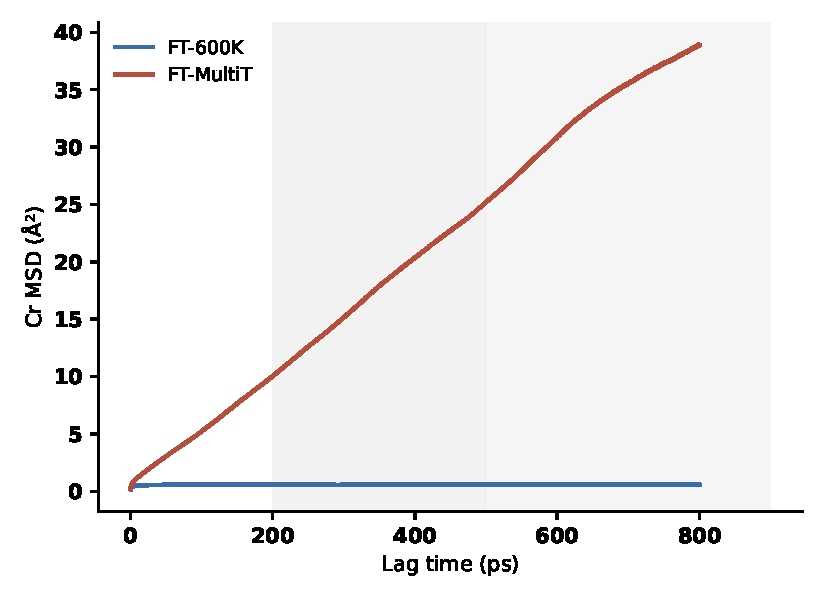
\includegraphics[width=\linewidth,height=0.42\textheight,keepaspectratio]{figure_pages/assets/fig_065.pdf}
\caption{Legacy one-nanosecond molecular-dynamics diagnostics retained for provenance comparison. This page shows the candidate output ``Fig msd'' within the audited MD-1NS-LEGACY family. The panel identity, source scope, and current status are retained in the accompanying evidence matrix.}
\label{fig:candidate_065}
\end{figure}
\textbf{Results text draft.} The figure records an earlier diagnostic view of the molecular-dynamics campaign and is useful for tracing how the analysis evolved. It is not automatically equivalent to the matched-protocol re-analysis.
\textbf{Discussion and boundary.} Use as historical or audit material only unless the local manifest confirms the current protocol, seeds, trajectory completeness, and acceptance gates.
\textbf{Article placement.} Proposed article location: SI transport or audit appendix only.
\textbf{Reviewer linkage:} overall status PENDING.
\begin{itemize}[leftmargin=1.4em,noitemsep]
\item \textbf{REV-C9 (PENDING):} Resolve the asymmetric FT-600K MD transport protocol and its effect on D and kappa. \emph{Completed:} Legacy FT-600K transport values are quarantined and excluded from ranking; the figure can document that boundary. \emph{Still required:} Run the corrected matched-protocol FT-600K long trajectory, block-average D/kappa, and close the multi-seed uncertainty before reporting a final transport comparison.
\end{itemize}
\textbf{Evidence pointers.}
\begin{itemize}[leftmargin=1.4em,noitemsep]
\item Data/processed: \begingroup\scriptsize\url{main/md_continuation_20260930/analysis_publication_20261003/audit.json}\endgroup
\item Data/processed: \begingroup\scriptsize\url{main/md_continuation_20260930/analysis_publication_20261003/figures/model_name_map.json}\endgroup
\item Plot/processing script: \begingroup\scriptsize\url{main/md_continuation_20260930/analysis_publication_20261003/make_publication_artifacts.py}\endgroup
\item Caption/text source: \begingroup\scriptsize\url{main/md_continuation_20260930/analysis_publication_20261003/figures/table_stability_diffusion.tex}\endgroup
\end{itemize}
\statusline{\textbf{Audit gap / next action:} Retain as legacy until its source trajectory and renderer are matched to the 1-ns package}
\vfill
\clearpage
\section{FIG-066 --- Fig stability}
\label{figpage:fig-066}
\textbf{Group:} MD-1NS-LEGACY\quad \textbf{Evidence chain:} partial\quad \textbf{Status:} publication
\begin{figure}[H]
\centering
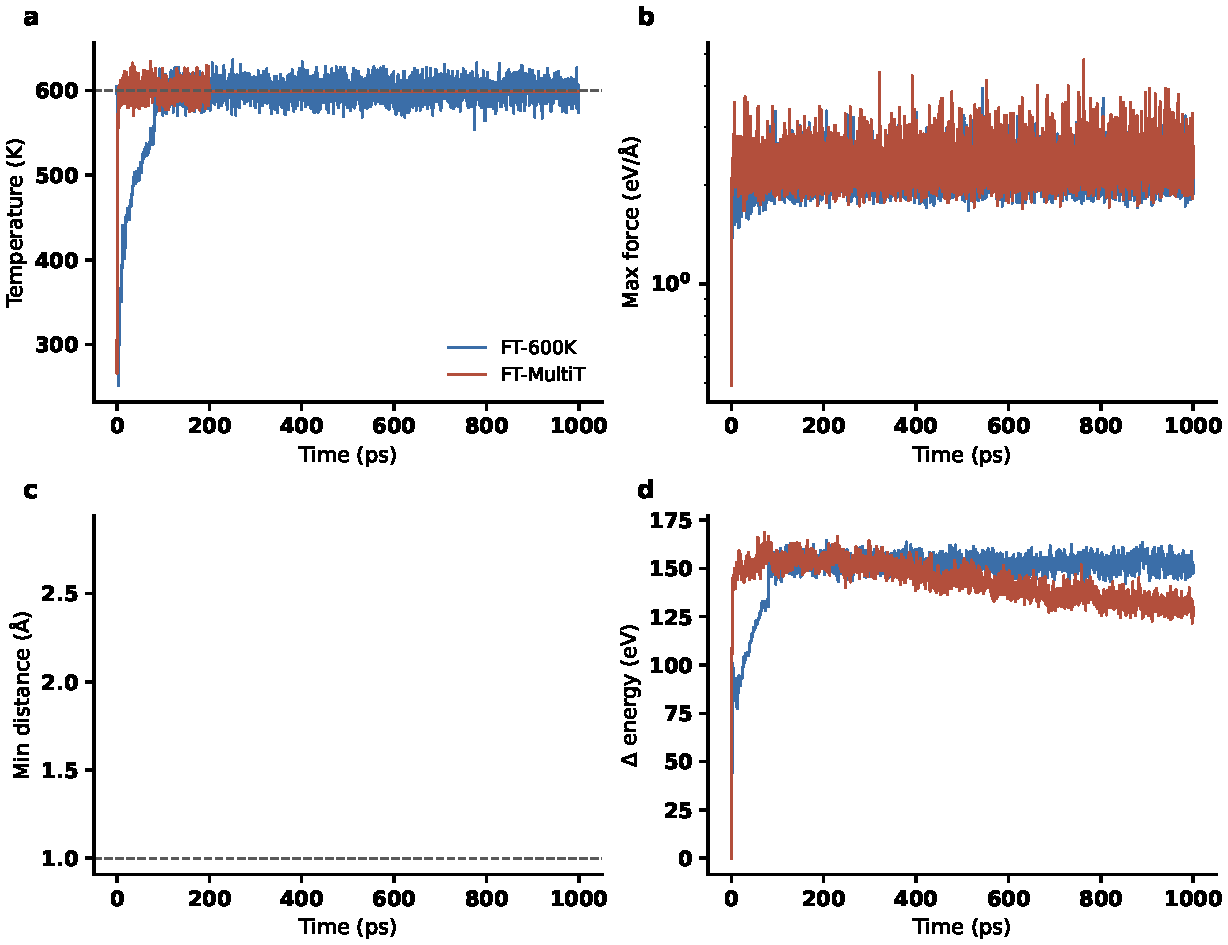
\includegraphics[width=\linewidth,height=0.42\textheight,keepaspectratio]{figure_pages/assets/fig_066.pdf}
\caption{Legacy one-nanosecond molecular-dynamics diagnostics retained for provenance comparison. This page shows the candidate output ``Fig stability'' within the audited MD-1NS-LEGACY family. The panel identity, source scope, and current status are retained in the accompanying evidence matrix.}
\label{fig:candidate_066}
\end{figure}
\textbf{Results text draft.} The figure records an earlier diagnostic view of the molecular-dynamics campaign and is useful for tracing how the analysis evolved. It is not automatically equivalent to the matched-protocol re-analysis.
\textbf{Discussion and boundary.} Use as historical or audit material only unless the local manifest confirms the current protocol, seeds, trajectory completeness, and acceptance gates.
\textbf{Article placement.} Proposed article location: SI transport or audit appendix only.
\textbf{Reviewer linkage:} overall status PENDING.
\begin{itemize}[leftmargin=1.4em,noitemsep]
\item \textbf{REV-C9 (PENDING):} Resolve the asymmetric FT-600K MD transport protocol and its effect on D and kappa. \emph{Completed:} Legacy FT-600K transport values are quarantined and excluded from ranking; the figure can document that boundary. \emph{Still required:} Run the corrected matched-protocol FT-600K long trajectory, block-average D/kappa, and close the multi-seed uncertainty before reporting a final transport comparison.
\end{itemize}
\textbf{Evidence pointers.}
\begin{itemize}[leftmargin=1.4em,noitemsep]
\item Data/processed: \begingroup\scriptsize\url{main/md_continuation_20260930/analysis_publication_20261003/audit.json}\endgroup
\item Data/processed: \begingroup\scriptsize\url{main/md_continuation_20260930/analysis_publication_20261003/figures/model_name_map.json}\endgroup
\item Plot/processing script: \begingroup\scriptsize\url{main/md_continuation_20260930/analysis_publication_20261003/make_publication_artifacts.py}\endgroup
\item Caption/text source: \begingroup\scriptsize\url{main/md_continuation_20260930/analysis_publication_20261003/figures/table_stability_diffusion.tex}\endgroup
\end{itemize}
\statusline{\textbf{Audit gap / next action:} Retain as legacy until its source trajectory and renderer are matched to the 1-ns package}
\vfill
\clearpage
\section{FIG-067 --- Fig vacf}
\label{figpage:fig-067}
\textbf{Group:} MD-1NS-LEGACY\quad \textbf{Evidence chain:} partial\quad \textbf{Status:} publication
\begin{figure}[H]
\centering
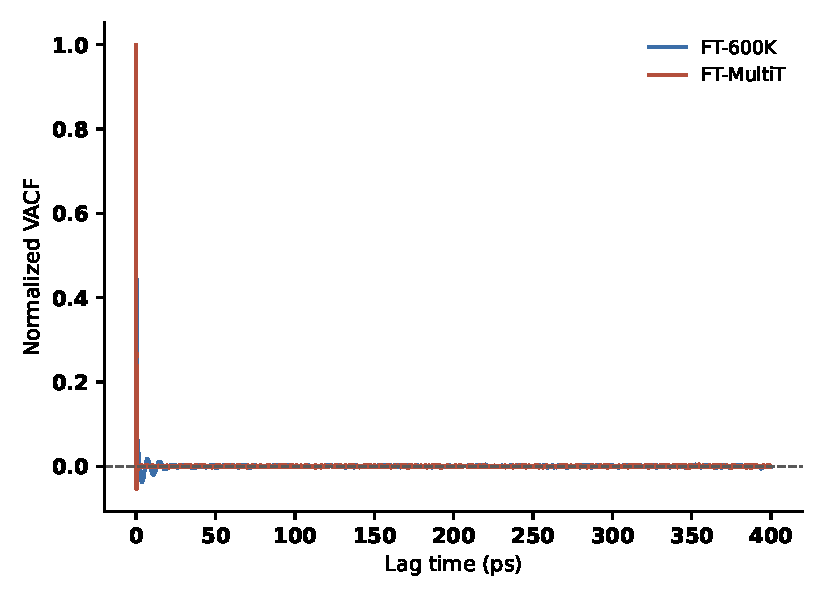
\includegraphics[width=\linewidth,height=0.42\textheight,keepaspectratio]{figure_pages/assets/fig_067.pdf}
\caption{Legacy one-nanosecond molecular-dynamics diagnostics retained for provenance comparison. This page shows the candidate output ``Fig vacf'' within the audited MD-1NS-LEGACY family. The panel identity, source scope, and current status are retained in the accompanying evidence matrix.}
\label{fig:candidate_067}
\end{figure}
\textbf{Results text draft.} The figure records an earlier diagnostic view of the molecular-dynamics campaign and is useful for tracing how the analysis evolved. It is not automatically equivalent to the matched-protocol re-analysis.
\textbf{Discussion and boundary.} Use as historical or audit material only unless the local manifest confirms the current protocol, seeds, trajectory completeness, and acceptance gates.
\textbf{Article placement.} Proposed article location: SI transport or audit appendix only.
\textbf{Reviewer linkage:} overall status PENDING.
\begin{itemize}[leftmargin=1.4em,noitemsep]
\item \textbf{REV-C9 (PENDING):} Resolve the asymmetric FT-600K MD transport protocol and its effect on D and kappa. \emph{Completed:} Legacy FT-600K transport values are quarantined and excluded from ranking; the figure can document that boundary. \emph{Still required:} Run the corrected matched-protocol FT-600K long trajectory, block-average D/kappa, and close the multi-seed uncertainty before reporting a final transport comparison.
\end{itemize}
\textbf{Evidence pointers.}
\begin{itemize}[leftmargin=1.4em,noitemsep]
\item Data/processed: \begingroup\scriptsize\url{main/md_continuation_20260930/analysis_publication_20261003/audit.json}\endgroup
\item Data/processed: \begingroup\scriptsize\url{main/md_continuation_20260930/analysis_publication_20261003/figures/model_name_map.json}\endgroup
\item Plot/processing script: \begingroup\scriptsize\url{main/md_continuation_20260930/analysis_publication_20261003/make_publication_artifacts.py}\endgroup
\item Caption/text source: \begingroup\scriptsize\url{main/md_continuation_20260930/analysis_publication_20261003/figures/table_stability_diffusion.tex}\endgroup
\end{itemize}
\statusline{\textbf{Audit gap / next action:} Retain as legacy until its source trajectory and renderer are matched to the 1-ns package}
\vfill
\clearpage
\section{FIG-068 --- Figure1 diffusion aware evaluation}
\label{figpage:fig-068}
\textbf{Group:} FIG-1-DIFFUSION\quad \textbf{Evidence chain:} traceable\quad \textbf{Status:} unclassified
\begin{figure}[H]
\centering
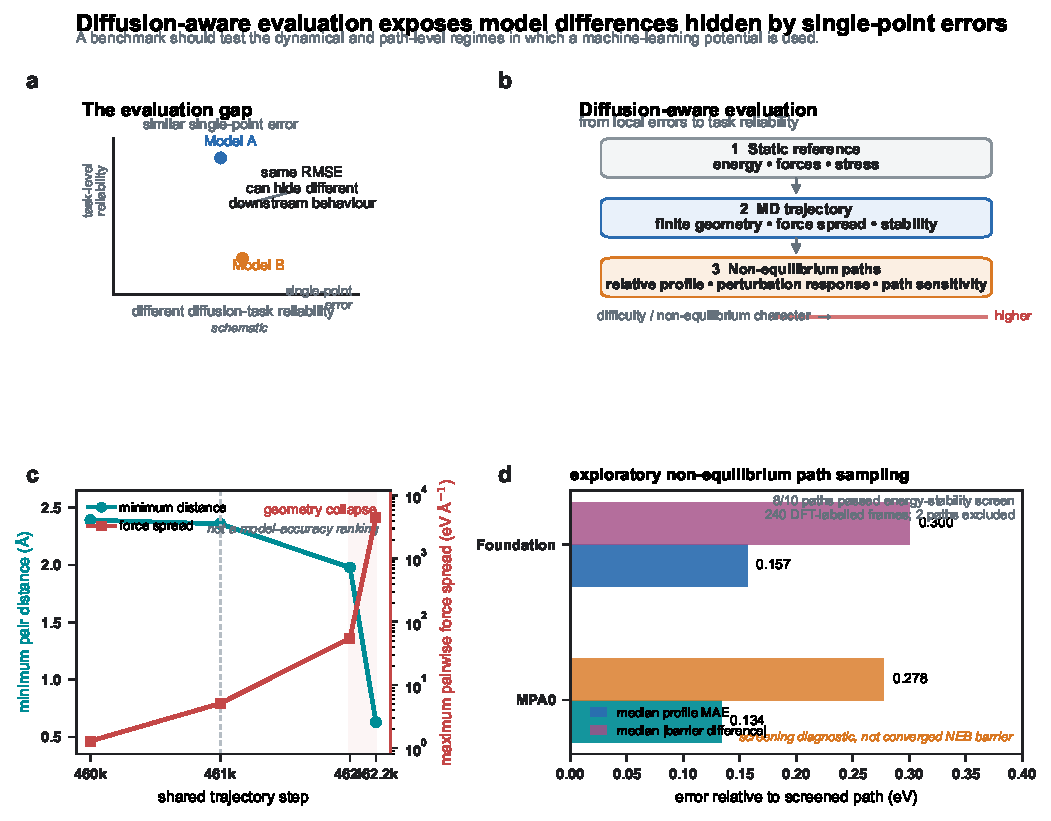
\includegraphics[width=\linewidth,height=0.42\textheight,keepaspectratio]{figure_pages/assets/fig_068.pdf}
\caption{Diffusion-aware benchmark framing, connecting the motivation, the evaluation protocol, and the audited dynamic evidence. This page shows the candidate output ``Figure1 diffusion aware evaluation'' within the audited FIG-1-DIFFUSION family. The panel identity, source scope, and current status are retained in the accompanying evidence matrix.}
\label{fig:candidate_068}
\end{figure}
\textbf{Results text draft.} This composite is intended to connect the benchmark question to the observable that is actually measured. It should be read as a context-to-result figure rather than as a claim that every downstream probe is converged.
\textbf{Discussion and boundary.} Use this figure at the Introduction/Results transition or as a high-level overview. The path-level and transport-level claims remain limited by the status fields recorded in the audit matrix.
\textbf{Article placement.} Proposed article location: Introduction/Results transition; diffusion-aware evaluation.
\textbf{Reviewer linkage:} overall status DONE.
\begin{itemize}[leftmargin=1.4em,noitemsep]
\item \textbf{REV-A4 (DONE):} Rescope generalizability claims or add an independent material/dopant validation. \emph{Completed:} The manuscript language is scoped to a candidate framework demonstrated on Cr-doped Sb2Te3; broader claims are framed as future validation. \emph{Still required:} Do not add a cross-system conclusion unless the optional second-dopant calculation is actually completed and audited.
\end{itemize}
\textbf{Evidence pointers.}
\begin{itemize}[leftmargin=1.4em,noitemsep]
\item Plot/processing script: \begingroup\scriptsize\url{ablation/analysis/figure1_context_method_result_20261002/figure1_nature.py}\endgroup
\item Caption/text source: \begingroup\scriptsize\url{ablation/analysis/figure1_context_method_result_20261002/figures/figure1_caption.md}\endgroup
\end{itemize}
\statusline{\textbf{Audit gap / next action:} Not yet mapped to the revision1 TeX figure labels}
\vfill
\clearpage
\section{FIG-069 --- Screening plot atlas msd dxy}
\label{figpage:fig-069}
\textbf{Group:} MD-ABLATION-20PS\quad \textbf{Evidence chain:} traceable\quad \textbf{Status:} unclassified
\begin{figure}[H]
\centering
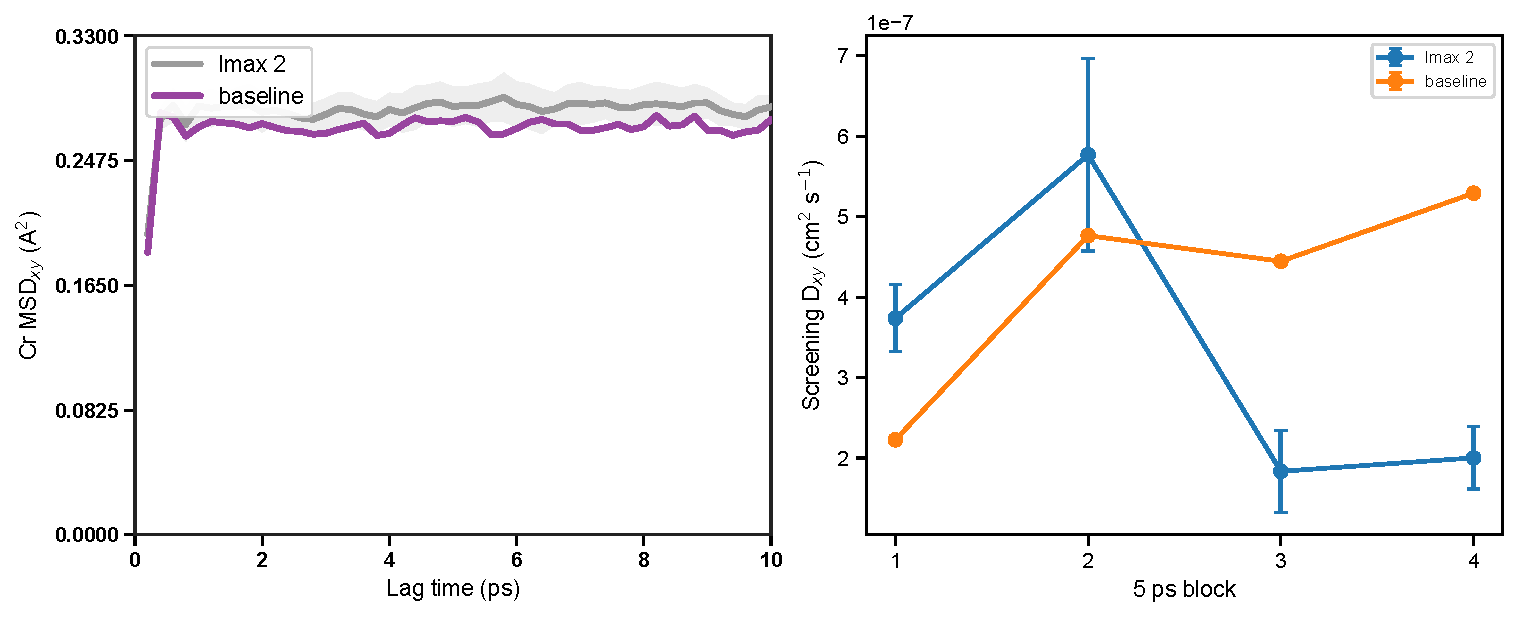
\includegraphics[width=\linewidth,height=0.42\textheight,keepaspectratio]{figure_pages/assets/fig_069.pdf}
\caption{From-scratch ablation screening under the declared short-time molecular-dynamics protocol. This page shows the candidate output ``Screening plot atlas msd dxy'' within the audited MD-ABLATION-20PS family. The panel identity, source scope, and current status are retained in the accompanying evidence matrix.}
\label{fig:candidate_069}
\end{figure}
\textbf{Results text draft.} The ablation panels distinguish complete short screening trajectories from early scientific instability and launcher/resource failures. The screening outcome is therefore a model/protocol triage signal, not a formal transport result.
\textbf{Discussion and boundary.} The 20 ps screen supports selection and failure analysis. It does not replace the pending accepted 1 ns campaign and must not be used to report Dxy, HFACF, or kappa for failed branches.
\textbf{Article placement.} Proposed article location: Results/SI: ablation stability and transport-screen boundary.
\textbf{Reviewer linkage:} overall status PARTIAL.
\begin{itemize}[leftmargin=1.4em,noitemsep]
\item \textbf{REV-C9 (PENDING):} Resolve the asymmetric FT-600K MD transport protocol and its effect on D and kappa. \emph{Completed:} Legacy FT-600K transport values are quarantined and excluded from ranking; the figure can document that boundary. \emph{Still required:} Run the corrected matched-protocol FT-600K long trajectory, block-average D/kappa, and close the multi-seed uncertainty before reporting a final transport comparison.
\item \textbf{REV-A3 (PARTIAL):} Add seed-level uncertainty and test whether the deep-penetration result is seed-stable rather than a chance outcome. \emph{Completed:} Three-seed grouped in-gap comparisons and uncertainty are available for the declared Scratch/FT-600K/Scratch-5\% scope. \emph{Still required:} Complete path-resolved deep-penetration classification and restarted QE references before reporting a pooled deep-penetration ranking.
\item \textbf{REV-A5 (PARTIAL):} Add a Scratch-5\% random-initialization control to separate foundation pretraining from data-volume effects. \emph{Completed:} The three-seed Scratch-5\% control and the in-gap pathway comparison are complete and can be shown with the stated small-sample caveat. \emph{Still required:} Do not generalize to FT-MultiT or all pathways until the corresponding grouped retraining and path comparisons exist.
\end{itemize}
\textbf{Evidence pointers.}
\begin{itemize}[leftmargin=1.4em,noitemsep]
\item Data/processed: \begingroup\scriptsize\url{ablation/analysis/from_scratch_ablation_md_20261005/campaign_manifest.json}\endgroup
\item Data/processed: \begingroup\scriptsize\url{ablation/analysis/from_scratch_ablation_md_20261005/comparison_inventory.csv}\endgroup
\item Plot/processing script: \begingroup\scriptsize\url{ablation/analysis/from_scratch_ablation_md_20261005/analyze_ablation_md.py}\endgroup
\item Plot/processing script: \begingroup\scriptsize\url{ablation/analysis/from_scratch_ablation_md_20261005/analyze_production_uncertainty.py}\endgroup
\item Caption/text source: \begingroup\scriptsize\url{ablation/analysis/from_scratch_ablation_md_20261005/20ps_screening_report.md}\endgroup
\item Caption/text source: \begingroup\scriptsize\url{ablation/analysis/from_scratch_ablation_md_20261005/PROTOCOL_AND_COMPARISON.md}\endgroup
\end{itemize}
\statusline{\textbf{Audit gap / next action:} 20 ps/1 ns acceptance and formal transport gates remain incomplete; preserve failed branches and velocity/training-seed separation}
\vfill
\clearpage
\section{FIG-070 --- Md unified comparison}
\label{figpage:fig-070}
\textbf{Group:} MD-ABLATION-20PS\quad \textbf{Evidence chain:} traceable\quad \textbf{Status:} comparison
\begin{figure}[H]
\centering
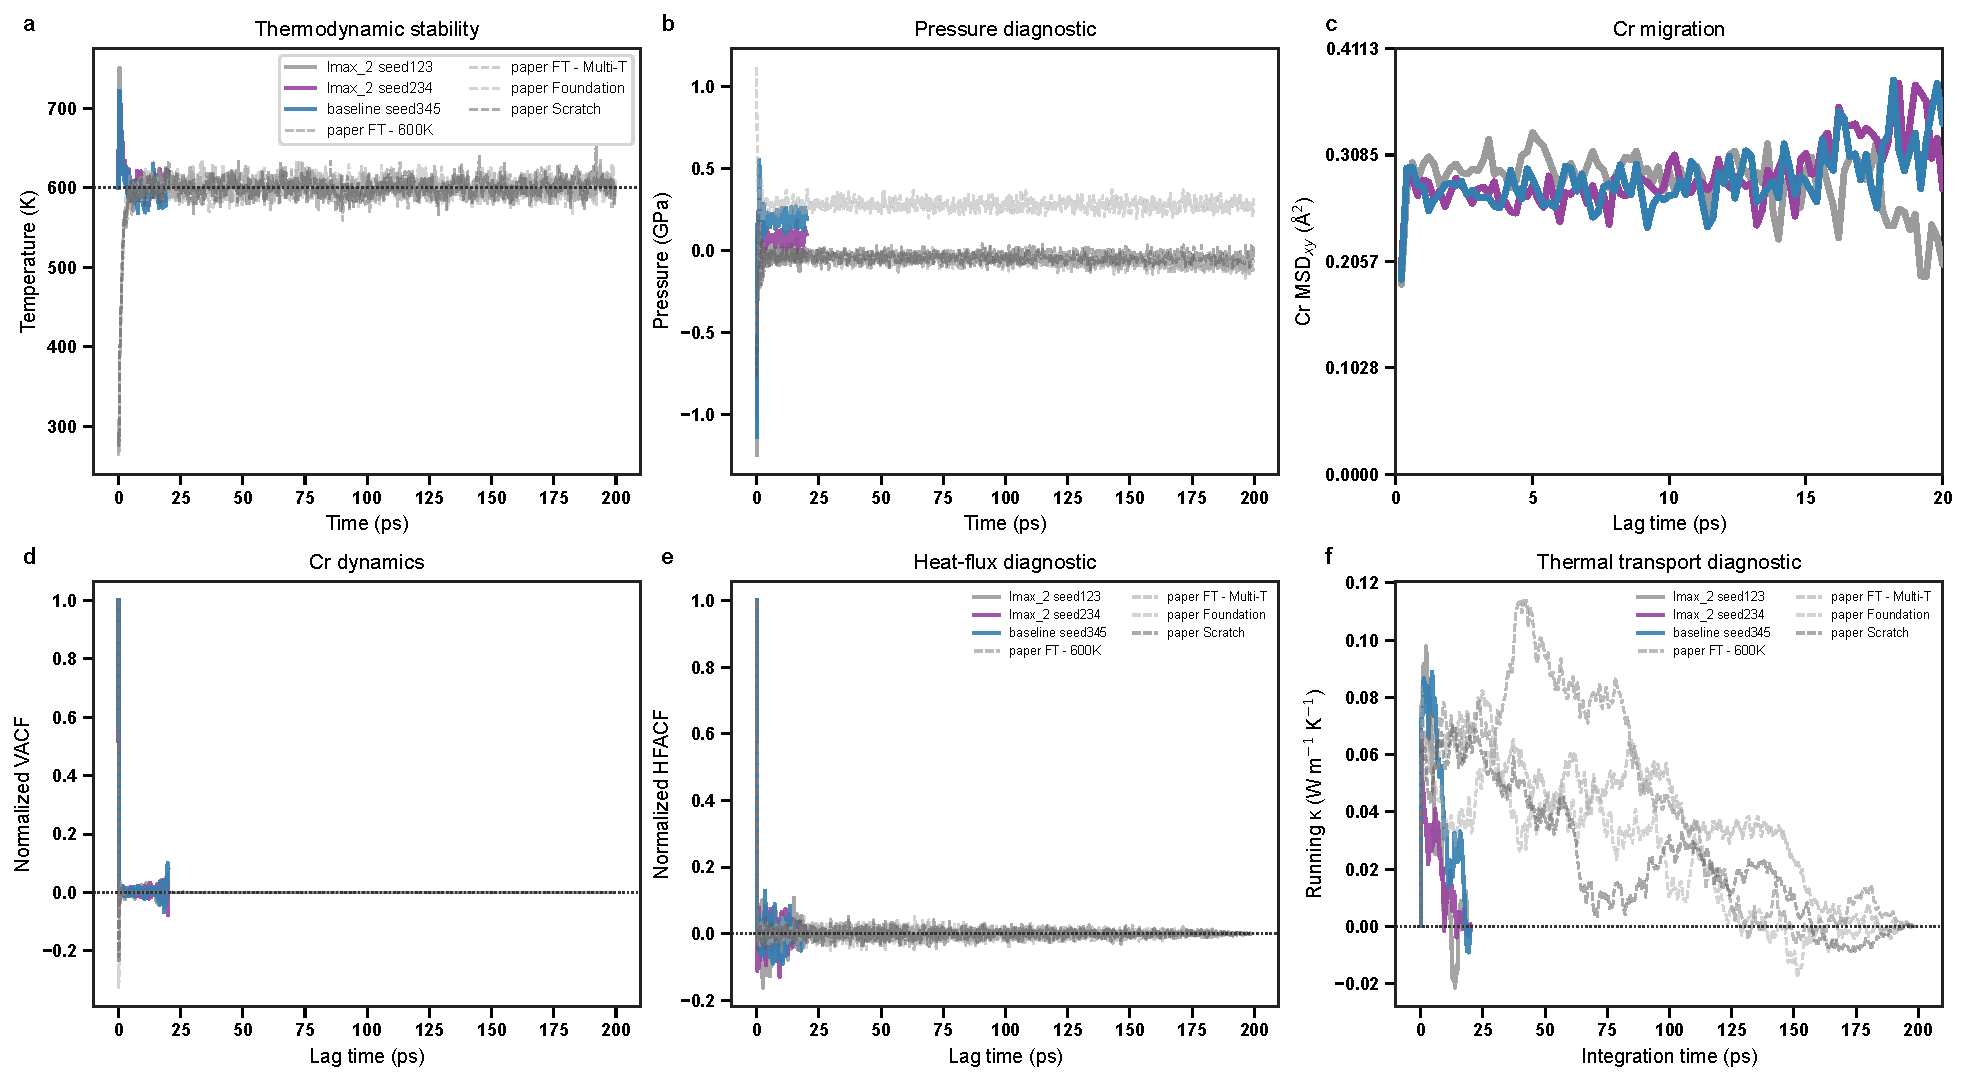
\includegraphics[width=\linewidth,height=0.42\textheight,keepaspectratio]{figure_pages/assets/fig_070.pdf}
\caption{From-scratch ablation screening under the declared short-time molecular-dynamics protocol. This page shows the candidate output ``Md unified comparison'' within the audited MD-ABLATION-20PS family. The panel identity, source scope, and current status are retained in the accompanying evidence matrix.}
\label{fig:candidate_070}
\end{figure}
\textbf{Results text draft.} The ablation panels distinguish complete short screening trajectories from early scientific instability and launcher/resource failures. The screening outcome is therefore a model/protocol triage signal, not a formal transport result.
\textbf{Discussion and boundary.} The 20 ps screen supports selection and failure analysis. It does not replace the pending accepted 1 ns campaign and must not be used to report Dxy, HFACF, or kappa for failed branches.
\textbf{Article placement.} Proposed article location: Results/SI: ablation stability and transport-screen boundary.
\textbf{Reviewer linkage:} overall status PARTIAL.
\begin{itemize}[leftmargin=1.4em,noitemsep]
\item \textbf{REV-A3 (PARTIAL):} Add seed-level uncertainty and test whether the deep-penetration result is seed-stable rather than a chance outcome. \emph{Completed:} Three-seed grouped in-gap comparisons and uncertainty are available for the declared Scratch/FT-600K/Scratch-5\% scope. \emph{Still required:} Complete path-resolved deep-penetration classification and restarted QE references before reporting a pooled deep-penetration ranking.
\item \textbf{REV-A5 (PARTIAL):} Add a Scratch-5\% random-initialization control to separate foundation pretraining from data-volume effects. \emph{Completed:} The three-seed Scratch-5\% control and the in-gap pathway comparison are complete and can be shown with the stated small-sample caveat. \emph{Still required:} Do not generalize to FT-MultiT or all pathways until the corresponding grouped retraining and path comparisons exist.
\end{itemize}
\textbf{Evidence pointers.}
\begin{itemize}[leftmargin=1.4em,noitemsep]
\item Data/processed: \begingroup\scriptsize\url{ablation/analysis/from_scratch_ablation_md_20261005/campaign_manifest.json}\endgroup
\item Data/processed: \begingroup\scriptsize\url{ablation/analysis/from_scratch_ablation_md_20261005/comparison_inventory.csv}\endgroup
\item Plot/processing script: \begingroup\scriptsize\url{ablation/analysis/from_scratch_ablation_md_20261005/analyze_ablation_md.py}\endgroup
\item Plot/processing script: \begingroup\scriptsize\url{ablation/analysis/from_scratch_ablation_md_20261005/analyze_production_uncertainty.py}\endgroup
\item Caption/text source: \begingroup\scriptsize\url{ablation/analysis/from_scratch_ablation_md_20261005/20ps_screening_report.md}\endgroup
\item Caption/text source: \begingroup\scriptsize\url{ablation/analysis/from_scratch_ablation_md_20261005/PROTOCOL_AND_COMPARISON.md}\endgroup
\end{itemize}
\statusline{\textbf{Audit gap / next action:} 20 ps/1 ns acceptance and formal transport gates remain incomplete; preserve failed branches and velocity/training-seed separation}
\vfill
\clearpage
\section{FIG-071 --- Screening msd dxy}
\label{figpage:fig-071}
\textbf{Group:} MD-ABLATION-20PS\quad \textbf{Evidence chain:} traceable\quad \textbf{Status:} audit
\begin{figure}[H]
\centering
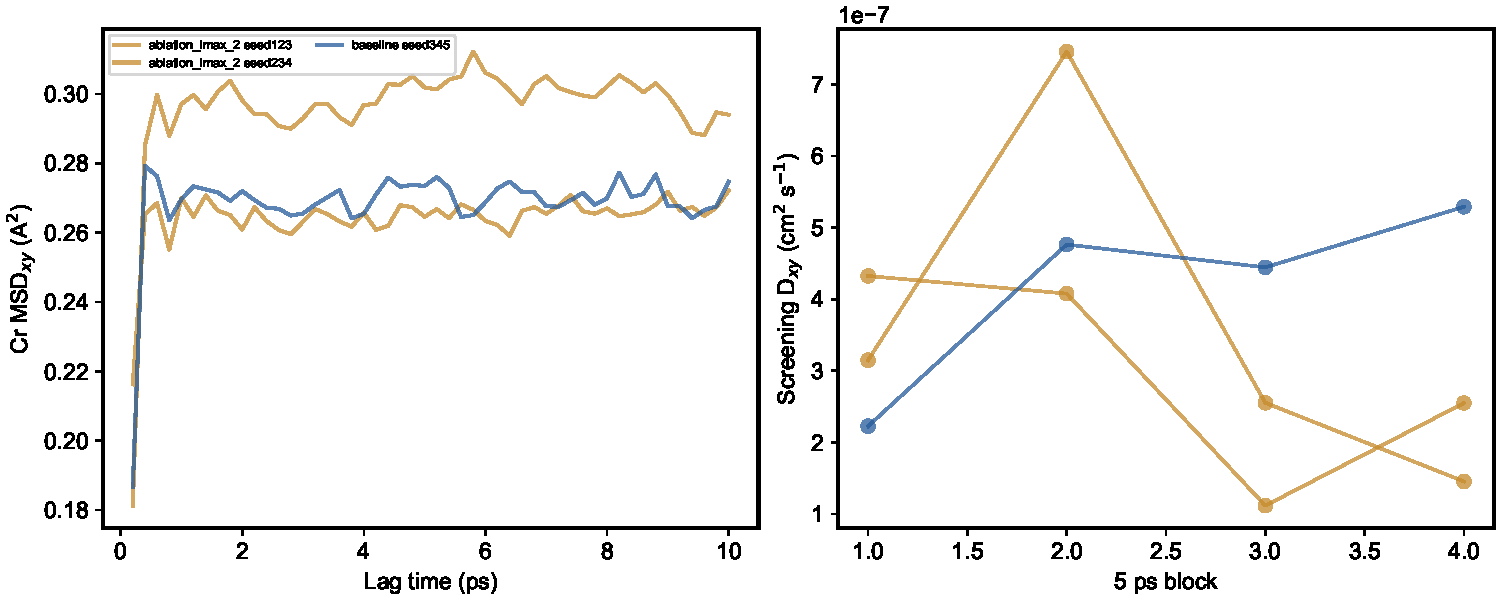
\includegraphics[width=\linewidth,height=0.42\textheight,keepaspectratio]{figure_pages/assets/fig_071.pdf}
\caption{From-scratch ablation screening under the declared short-time molecular-dynamics protocol. This page shows the candidate output ``Screening msd dxy'' within the audited MD-ABLATION-20PS family. The panel identity, source scope, and current status are retained in the accompanying evidence matrix.}
\label{fig:candidate_071}
\end{figure}
\textbf{Results text draft.} The ablation panels distinguish complete short screening trajectories from early scientific instability and launcher/resource failures. The screening outcome is therefore a model/protocol triage signal, not a formal transport result.
\textbf{Discussion and boundary.} The 20 ps screen supports selection and failure analysis. It does not replace the pending accepted 1 ns campaign and must not be used to report Dxy, HFACF, or kappa for failed branches.
\textbf{Article placement.} Proposed article location: Results/SI: ablation stability and transport-screen boundary.
\textbf{Reviewer linkage:} overall status PARTIAL.
\begin{itemize}[leftmargin=1.4em,noitemsep]
\item \textbf{REV-C9 (PENDING):} Resolve the asymmetric FT-600K MD transport protocol and its effect on D and kappa. \emph{Completed:} Legacy FT-600K transport values are quarantined and excluded from ranking; the figure can document that boundary. \emph{Still required:} Run the corrected matched-protocol FT-600K long trajectory, block-average D/kappa, and close the multi-seed uncertainty before reporting a final transport comparison.
\item \textbf{REV-A3 (PARTIAL):} Add seed-level uncertainty and test whether the deep-penetration result is seed-stable rather than a chance outcome. \emph{Completed:} Three-seed grouped in-gap comparisons and uncertainty are available for the declared Scratch/FT-600K/Scratch-5\% scope. \emph{Still required:} Complete path-resolved deep-penetration classification and restarted QE references before reporting a pooled deep-penetration ranking.
\item \textbf{REV-A5 (PARTIAL):} Add a Scratch-5\% random-initialization control to separate foundation pretraining from data-volume effects. \emph{Completed:} The three-seed Scratch-5\% control and the in-gap pathway comparison are complete and can be shown with the stated small-sample caveat. \emph{Still required:} Do not generalize to FT-MultiT or all pathways until the corresponding grouped retraining and path comparisons exist.
\end{itemize}
\textbf{Evidence pointers.}
\begin{itemize}[leftmargin=1.4em,noitemsep]
\item Data/processed: \begingroup\scriptsize\url{ablation/analysis/from_scratch_ablation_md_20261005/remote_20ps_audit/retry_ledger.tsv}\endgroup
\item Data/processed: \begingroup\scriptsize\url{ablation/analysis/from_scratch_ablation_md_20261005/remote_20ps_audit/screening_summary.csv}\endgroup
\end{itemize}
\statusline{\textbf{Audit gap / next action:} 20 ps/1 ns acceptance and formal transport gates remain incomplete; preserve failed branches and velocity/training-seed separation}
\vfill
\clearpage
\section{FIG-072 --- Fig1 endpoint robustness}
\label{figpage:fig-072}
\textbf{Group:} ENDPOINT-MACE\quad \textbf{Evidence chain:} traceable\quad \textbf{Status:} unclassified
\begin{figure}[H]
\centering
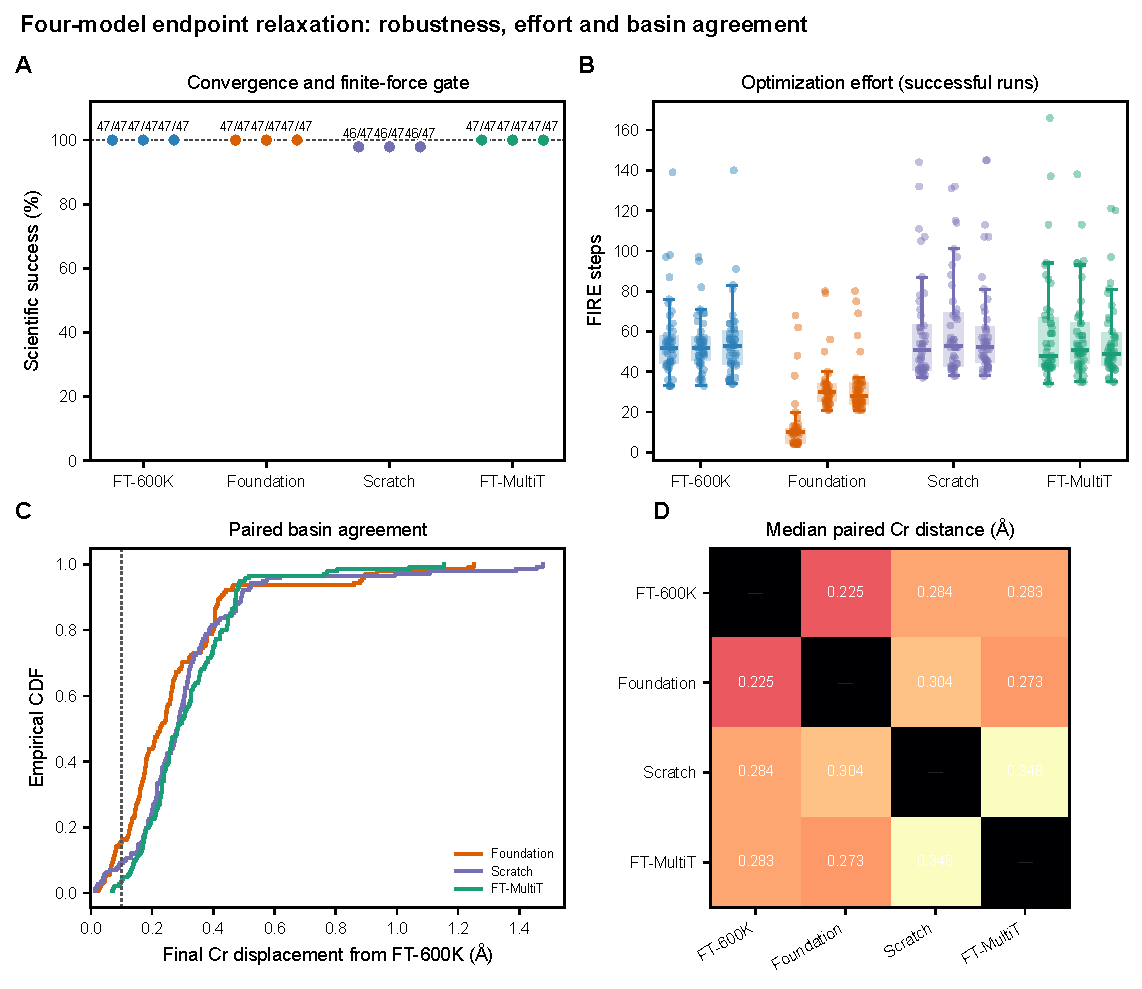
\includegraphics[width=\linewidth,height=0.42\textheight,keepaspectratio]{figure_pages/assets/fig_072.pdf}
\caption{Mace endpoint energy/force or relaxation comparison. This page shows the candidate output ``Fig1 endpoint robustness'' within the audited ENDPOINT-MACE family. The panel identity, source scope, and current status are retained in the accompanying evidence matrix.}
\label{fig:candidate_072}
\end{figure}
\textbf{Results text draft.} The figure compares endpoint behavior across the declared MACE model set and preserves the sampled endpoint identity. It is a local structural/energetic probe, not a transition-state calculation.
\textbf{Discussion and boundary.} Use to motivate model differences at endpoints, while keeping the separate path-level and DFT convergence limitations visible.
\textbf{Article placement.} Proposed article location: Results: endpoint robustness.
\textbf{Reviewer linkage:} overall status NO\_DIRECT\_REVIEWER\_FIGURE\_LINK.
No direct reviewer-response figure linkage was identified; this page is retained for scientific/article audit rather than as a direct reviewer response.
\textbf{Evidence pointers.}
\begin{itemize}[leftmargin=1.4em,noitemsep]
\item Data/processed: \begingroup\scriptsize\url{ablation/analysis/mace_endpoint_four_model/outputs/table_energy_span_by_endpoint.csv}\endgroup
\item Data/processed: \begingroup\scriptsize\url{ablation/analysis/mace_endpoint_four_model/outputs/table_model_agreement.csv}\endgroup
\item Plot/processing script: \begingroup\scriptsize\url{ablation/analysis/mace_endpoint_four_model/analyze_and_plot.py}\endgroup
\item Caption/text source: \begingroup\scriptsize\url{ablation/analysis/mace_endpoint_four_model/outputs/discussion_draft.md}\endgroup
\end{itemize}
\statusline{\textbf{Audit gap / next action:} Confirm current article section and whether endpoint task remains in the revision}
\vfill
\clearpage
\section{FIG-073 --- Fig2 relative energy landscape}
\label{figpage:fig-073}
\textbf{Group:} ENDPOINT-MACE\quad \textbf{Evidence chain:} traceable\quad \textbf{Status:} unclassified
\begin{figure}[H]
\centering
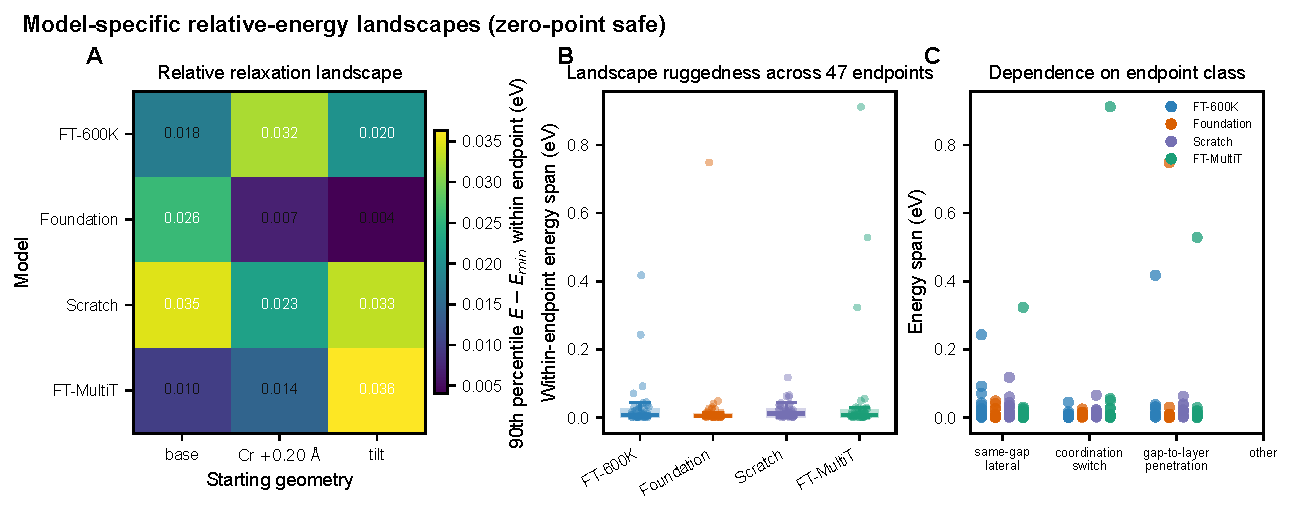
\includegraphics[width=\linewidth,height=0.42\textheight,keepaspectratio]{figure_pages/assets/fig_073.pdf}
\caption{Mace endpoint energy/force or relaxation comparison. This page shows the candidate output ``Fig2 relative energy landscape'' within the audited ENDPOINT-MACE family. The panel identity, source scope, and current status are retained in the accompanying evidence matrix.}
\label{fig:candidate_073}
\end{figure}
\textbf{Results text draft.} The figure compares endpoint behavior across the declared MACE model set and preserves the sampled endpoint identity. It is a local structural/energetic probe, not a transition-state calculation.
\textbf{Discussion and boundary.} Use to motivate model differences at endpoints, while keeping the separate path-level and DFT convergence limitations visible.
\textbf{Article placement.} Proposed article location: Results: endpoint robustness.
\textbf{Reviewer linkage:} overall status NO\_DIRECT\_REVIEWER\_FIGURE\_LINK.
No direct reviewer-response figure linkage was identified; this page is retained for scientific/article audit rather than as a direct reviewer response.
\textbf{Evidence pointers.}
\begin{itemize}[leftmargin=1.4em,noitemsep]
\item Data/processed: \begingroup\scriptsize\url{ablation/analysis/mace_endpoint_four_model/outputs/table_energy_span_by_endpoint.csv}\endgroup
\item Data/processed: \begingroup\scriptsize\url{ablation/analysis/mace_endpoint_four_model/outputs/table_model_agreement.csv}\endgroup
\item Plot/processing script: \begingroup\scriptsize\url{ablation/analysis/mace_endpoint_four_model/analyze_and_plot.py}\endgroup
\item Caption/text source: \begingroup\scriptsize\url{ablation/analysis/mace_endpoint_four_model/outputs/discussion_draft.md}\endgroup
\end{itemize}
\statusline{\textbf{Audit gap / next action:} Confirm current article section and whether endpoint task remains in the revision}
\vfill
\clearpage
\section{FIG-074 --- Time convergence}
\label{figpage:fig-074}
\textbf{Group:} MD-CONV\quad \textbf{Evidence chain:} partial\quad \textbf{Status:} unclassified
\begin{figure}[H]
\centering
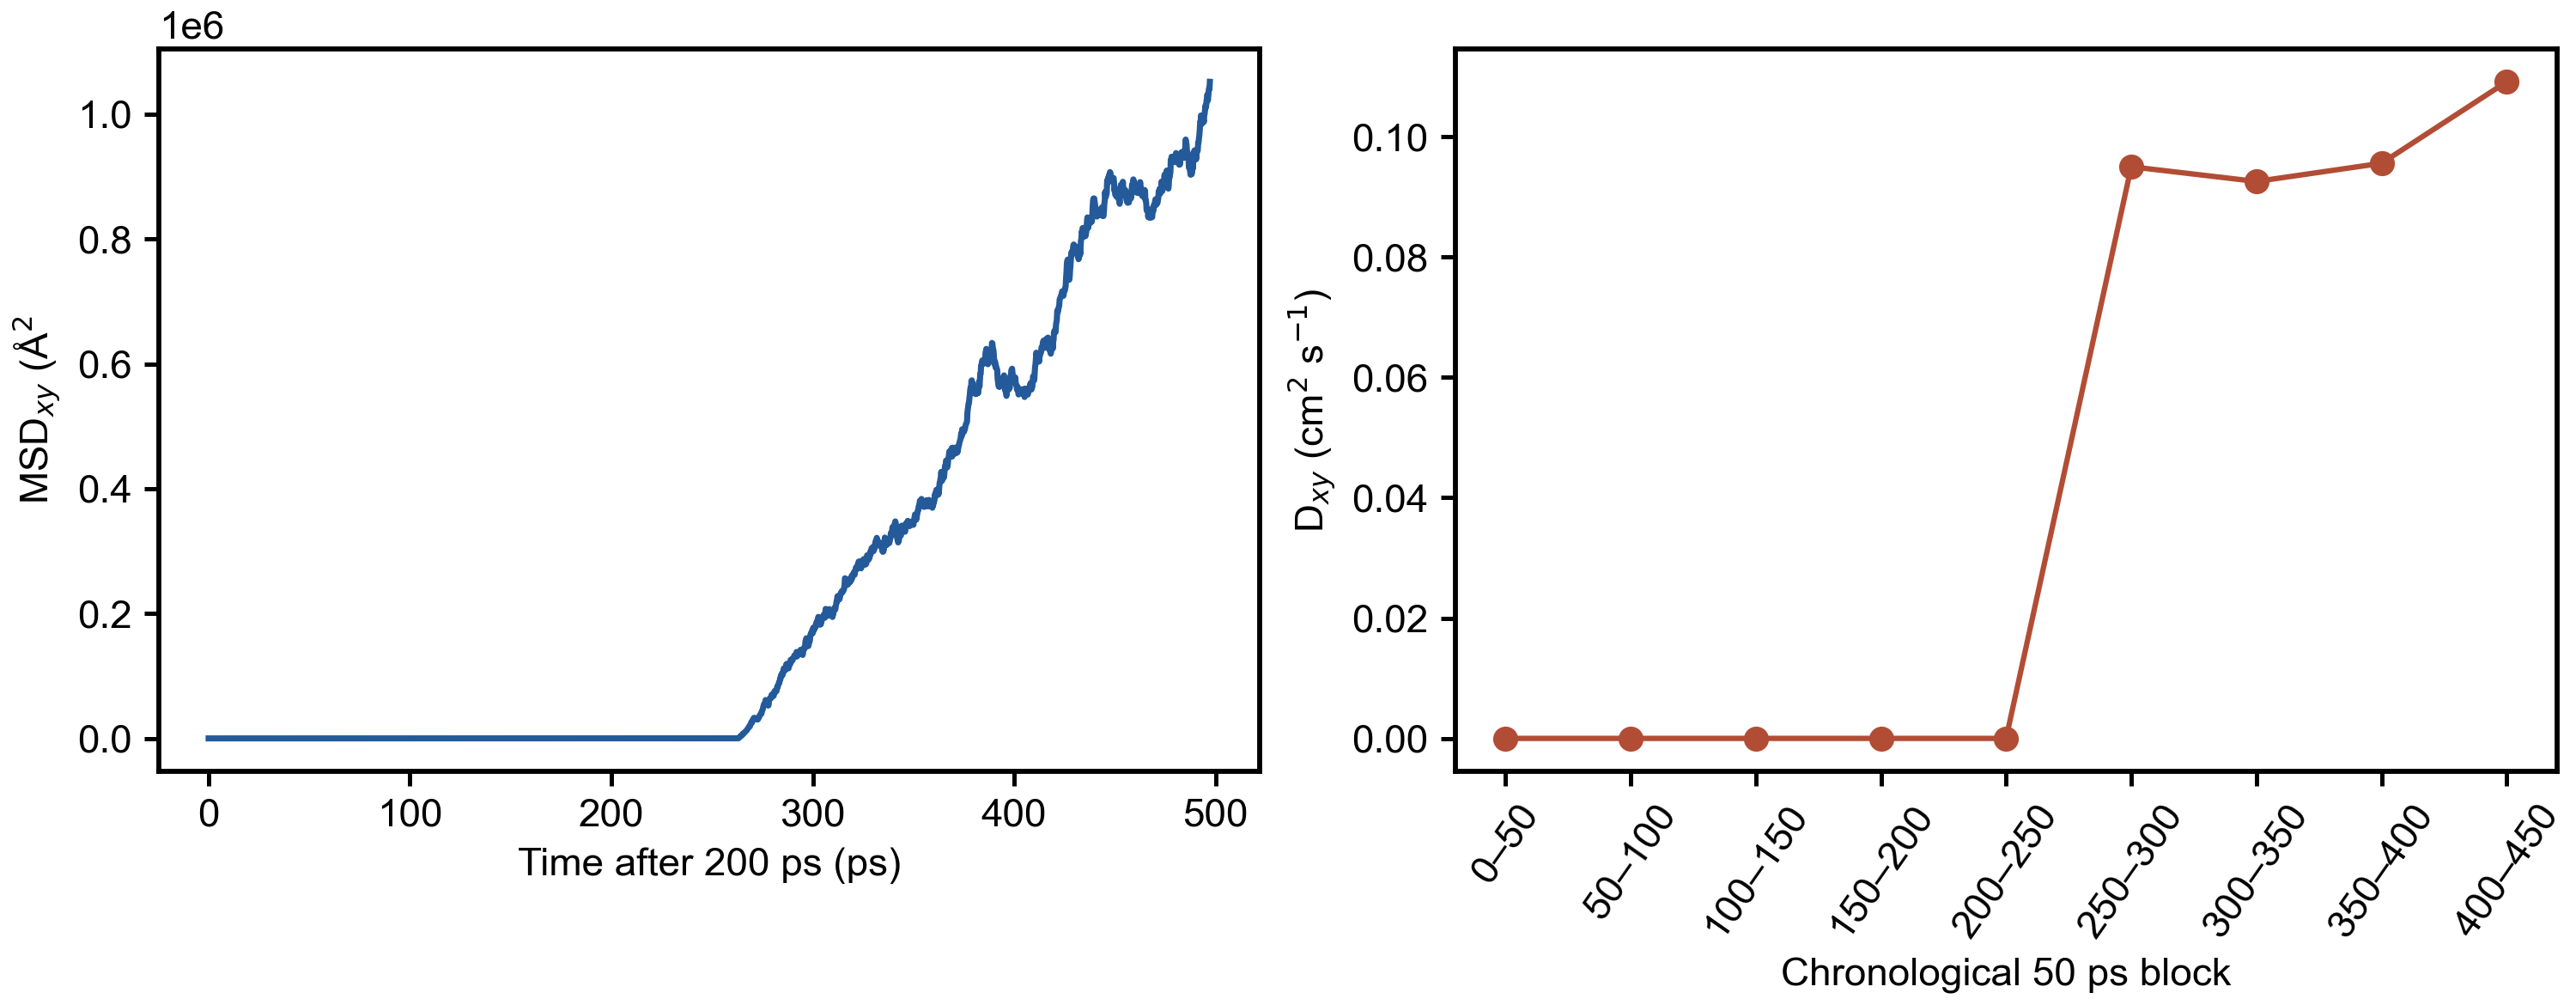
\includegraphics[width=\linewidth,height=0.42\textheight,keepaspectratio]{figure_pages/assets/fig_074.png}
\caption{Molecular-dynamics convergence, block statistics, or transport diagnostics. This page shows the candidate output ``Time convergence'' within the audited MD-CONV family. The panel identity, source scope, and current status are retained in the accompanying evidence matrix.}
\label{fig:candidate_074}
\end{figure}
\textbf{Results text draft.} The displayed curves or summaries show the convergence behavior and uncertainty treatment available in the corresponding source analysis. Only quantities backed by complete trajectories and the declared block protocol should enter manuscript ranking.
\textbf{Discussion and boundary.} Use for methods or SI validation. Short, mismatched, or provenance-only trajectories remain labeled as such and are excluded from formal cross-model conclusions.
\textbf{Article placement.} Proposed article location: SI transport-method validation.
\textbf{Reviewer linkage:} overall status PENDING.
\begin{itemize}[leftmargin=1.4em,noitemsep]
\item \textbf{REV-C9 (PENDING):} Resolve the asymmetric FT-600K MD transport protocol and its effect on D and kappa. \emph{Completed:} Legacy FT-600K transport values are quarantined and excluded from ranking; the figure can document that boundary. \emph{Still required:} Run the corrected matched-protocol FT-600K long trajectory, block-average D/kappa, and close the multi-seed uncertainty before reporting a final transport comparison.
\end{itemize}
\textbf{Evidence pointers.}
\begin{itemize}[leftmargin=1.4em,noitemsep]
\item Data/processed: \begingroup\scriptsize\url{ablation/analysis/mace_md_time_convergence_20261001/from-scratch/blocks_50ps.csv}\endgroup
\item Data/processed: \begingroup\scriptsize\url{ablation/analysis/mace_md_time_convergence_20261001/from-scratch/cumulative_windows.csv}\endgroup
\item Caption/text source: \begingroup\scriptsize\url{ablation/analysis/mace_md_time_convergence_20261001/REPORT.md}\endgroup
\end{itemize}
\statusline{\textbf{Audit gap / next action:} Plot script is not co-located with the image; map exact source generator}
\vfill
\clearpage
\section{FIG-075 --- Time convergence}
\label{figpage:fig-075}
\textbf{Group:} MD-CONV\quad \textbf{Evidence chain:} partial\quad \textbf{Status:} unclassified
\begin{figure}[H]
\centering
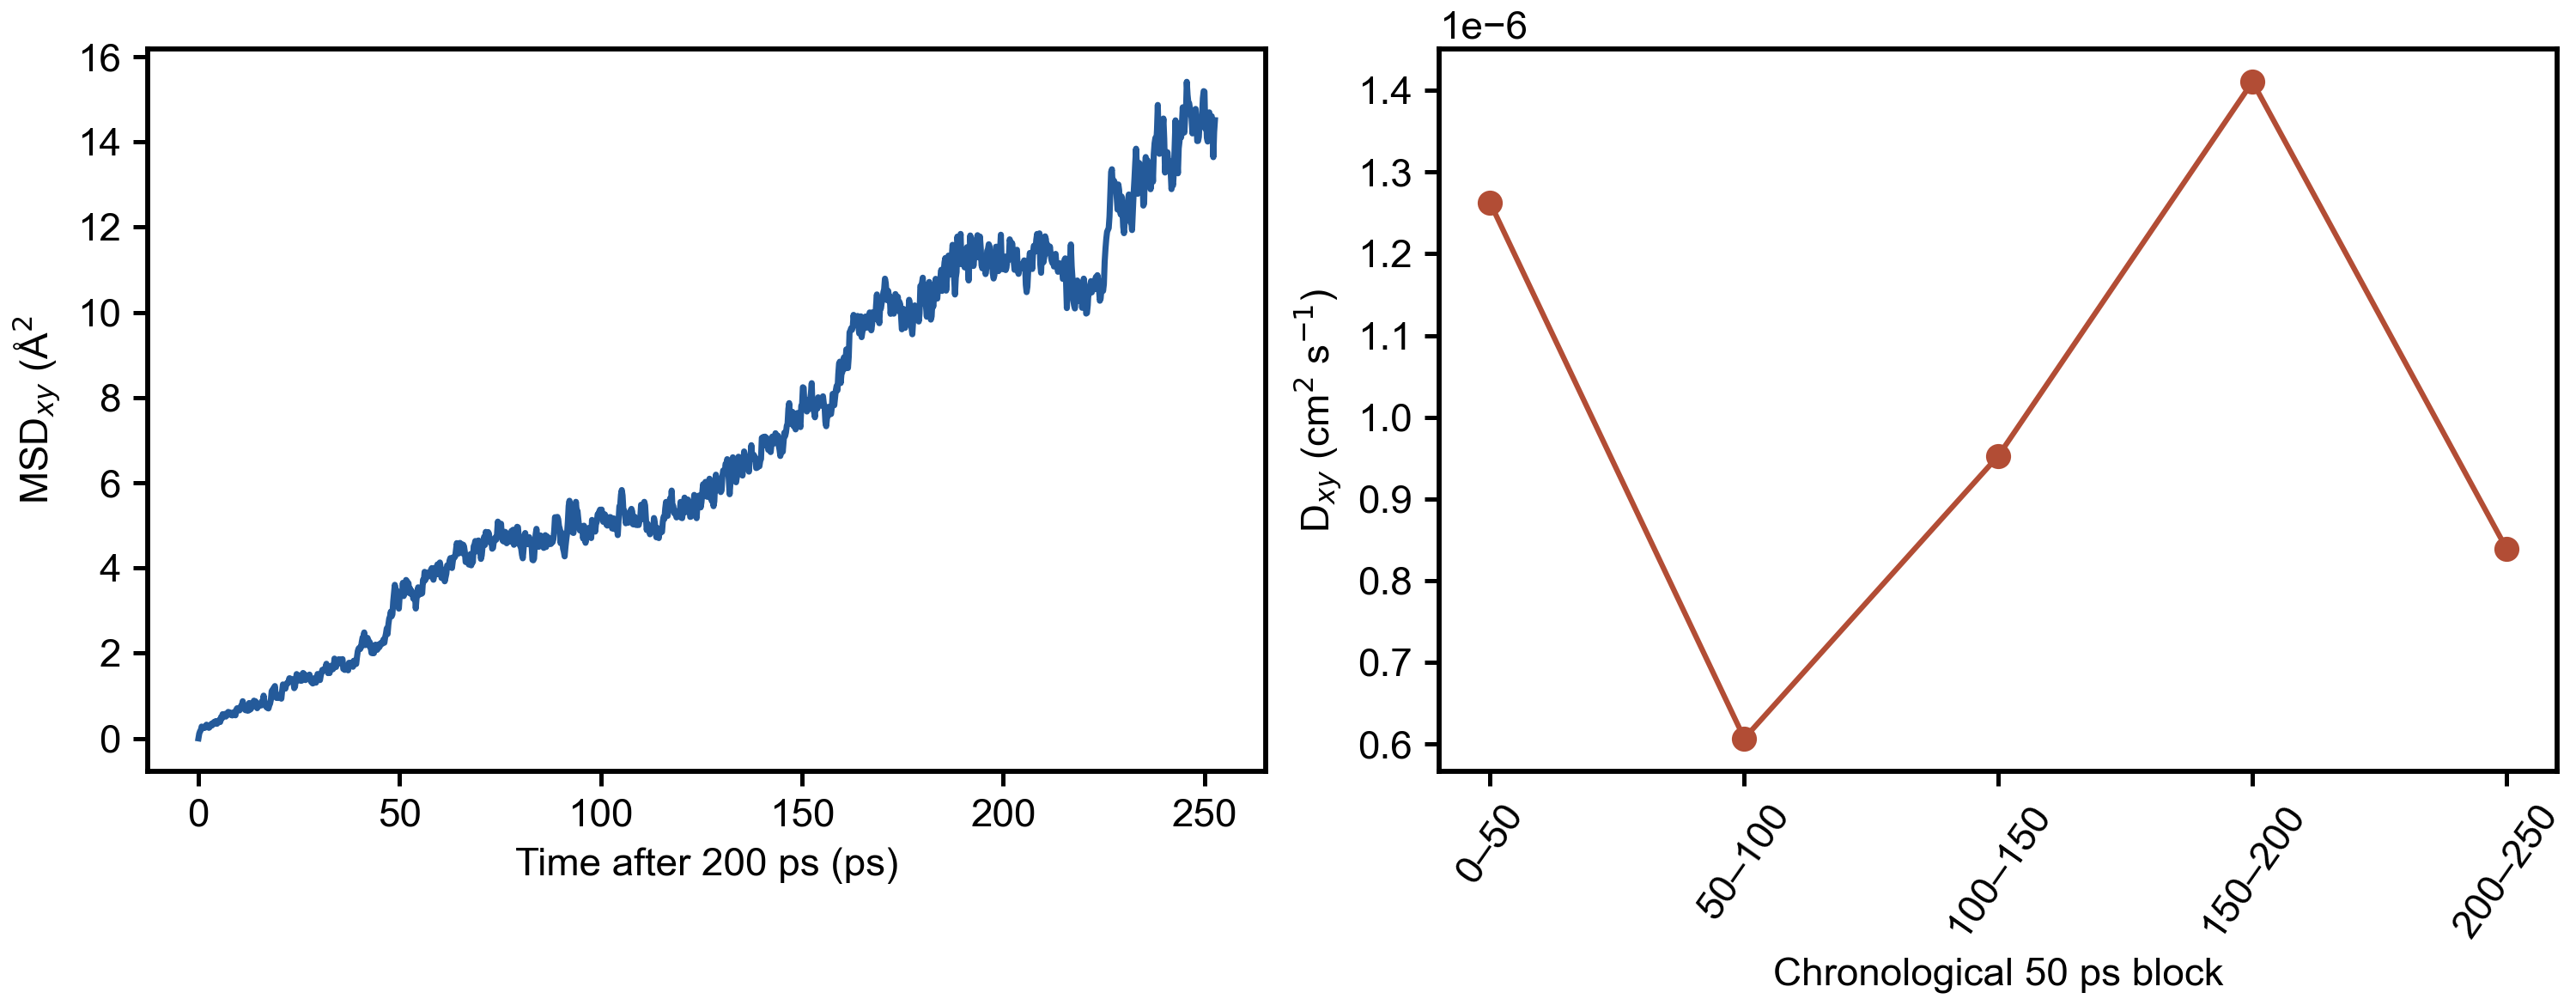
\includegraphics[width=\linewidth,height=0.42\textheight,keepaspectratio]{figure_pages/assets/fig_075.png}
\caption{Molecular-dynamics convergence, block statistics, or transport diagnostics. This page shows the candidate output ``Time convergence'' within the audited MD-CONV family. The panel identity, source scope, and current status are retained in the accompanying evidence matrix.}
\label{fig:candidate_075}
\end{figure}
\textbf{Results text draft.} The displayed curves or summaries show the convergence behavior and uncertainty treatment available in the corresponding source analysis. Only quantities backed by complete trajectories and the declared block protocol should enter manuscript ranking.
\textbf{Discussion and boundary.} Use for methods or SI validation. Short, mismatched, or provenance-only trajectories remain labeled as such and are excluded from formal cross-model conclusions.
\textbf{Article placement.} Proposed article location: SI transport-method validation.
\textbf{Reviewer linkage:} overall status PENDING.
\begin{itemize}[leftmargin=1.4em,noitemsep]
\item \textbf{REV-C9 (PENDING):} Resolve the asymmetric FT-600K MD transport protocol and its effect on D and kappa. \emph{Completed:} Legacy FT-600K transport values are quarantined and excluded from ranking; the figure can document that boundary. \emph{Still required:} Run the corrected matched-protocol FT-600K long trajectory, block-average D/kappa, and close the multi-seed uncertainty before reporting a final transport comparison.
\end{itemize}
\textbf{Evidence pointers.}
\begin{itemize}[leftmargin=1.4em,noitemsep]
\item Data/processed: \begingroup\scriptsize\url{ablation/analysis/mace_md_time_convergence_20261001/from_scratch_seg.tsv}\endgroup
\item Data/processed: \begingroup\scriptsize\url{ablation/analysis/mace_md_time_convergence_20261001/multi-T/blocks_50ps.csv}\endgroup
\item Caption/text source: \begingroup\scriptsize\url{ablation/analysis/mace_md_time_convergence_20261001/REPORT.md}\endgroup
\end{itemize}
\statusline{\textbf{Audit gap / next action:} Plot script is not co-located with the image; map exact source generator}
\vfill
\clearpage
\section{FIG-076 --- Fig1 force disagreement}
\label{figpage:fig-076}
\textbf{Group:} P1-FORCE\quad \textbf{Evidence chain:} traceable\quad \textbf{Status:} comparison
\begin{figure}[H]
\centering
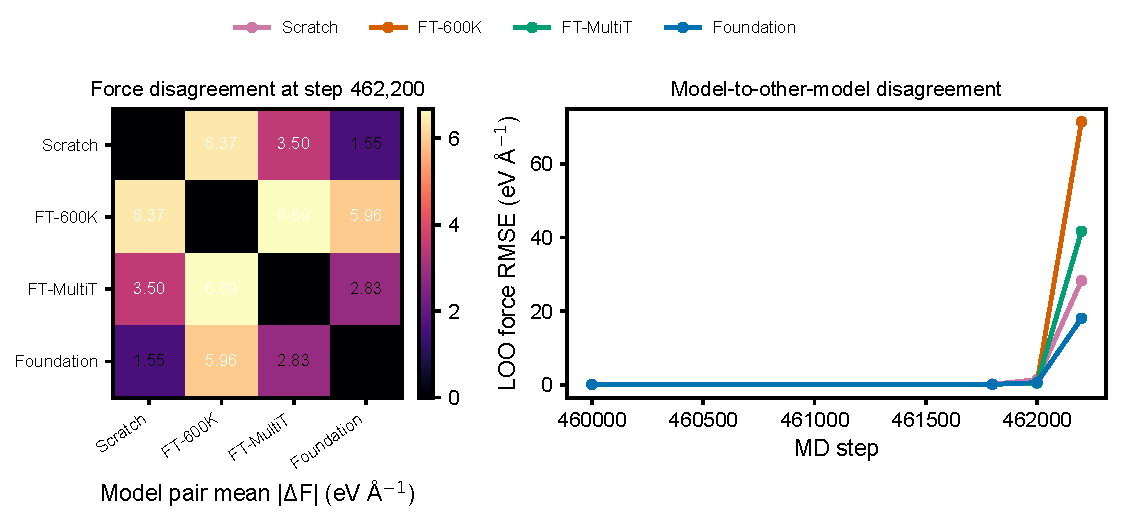
\includegraphics[width=\linewidth,height=0.42\textheight,keepaspectratio]{figure_pages/assets/fig_076.pdf}
\caption{Static force-disagreement and model-transfer diagnostics. This page shows the candidate output ``Fig1 force disagreement'' within the audited P1-FORCE family. The panel identity, source scope, and current status are retained in the accompanying evidence matrix.}
\label{fig:candidate_076}
\end{figure}
\textbf{Results text draft.} The figure compares model forces on a common set of configurations and exposes disagreement patterns that are not reducible to a single aggregate RMSE. The exact sampling scope and model provenance are retained in the evidence row.
\textbf{Discussion and boundary.} This supports the static-reference part of the benchmark. It does not by itself establish stability on a dynamically evolving path or agreement with converged DFT barriers.
\textbf{Article placement.} Proposed article location: Results: model disagreement and trajectory-integrity gate.
\textbf{Reviewer linkage:} overall status NO\_DIRECT\_REVIEWER\_FIGURE\_LINK.
No direct reviewer-response figure linkage was identified; this page is retained for scientific/article audit rather than as a direct reviewer response.
\textbf{Evidence pointers.}
\begin{itemize}[leftmargin=1.4em,noitemsep]
\item Data/processed: \begingroup\scriptsize\url{ablation/analysis/phase1_static_force_comparison_20261002/models_rockfish.json}\endgroup
\item Caption/text source: \begingroup\scriptsize\url{ablation/analysis/phase1_static_force_comparison_20261002/Methods.md}\endgroup
\item Caption/text source: \begingroup\scriptsize\url{ablation/analysis/phase1_static_force_comparison_20261002/README.md}\endgroup
\end{itemize}
\statusline{\textbf{Audit gap / next action:} Not yet integrated into the paper source}
\vfill
\clearpage
\section{FIG-077 --- Fig2 key local force}
\label{figpage:fig-077}
\textbf{Group:} P1-FORCE\quad \textbf{Evidence chain:} traceable\quad \textbf{Status:} comparison
\begin{figure}[H]
\centering
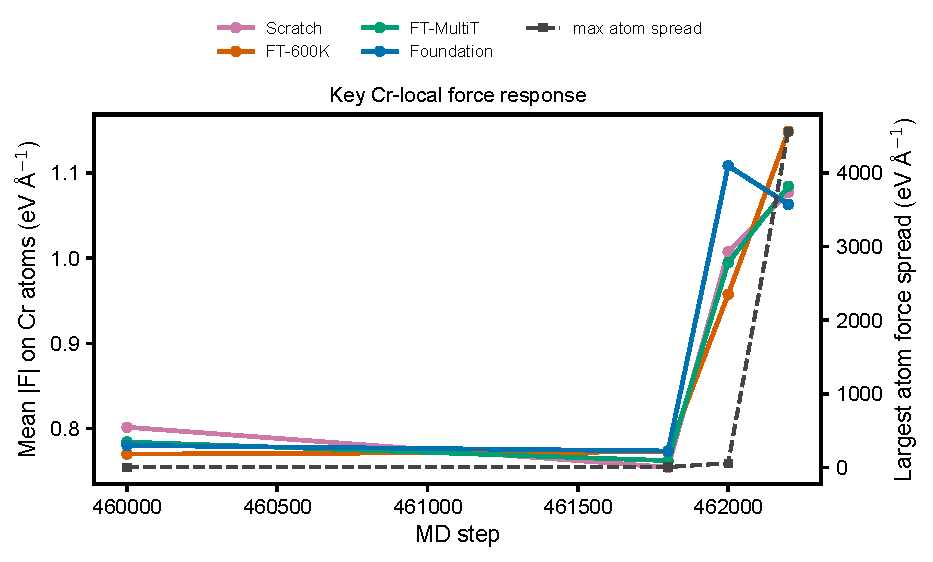
\includegraphics[width=\linewidth,height=0.42\textheight,keepaspectratio]{figure_pages/assets/fig_077.pdf}
\caption{Static force-disagreement and model-transfer diagnostics. This page shows the candidate output ``Fig2 key local force'' within the audited P1-FORCE family. The panel identity, source scope, and current status are retained in the accompanying evidence matrix.}
\label{fig:candidate_077}
\end{figure}
\textbf{Results text draft.} The figure compares model forces on a common set of configurations and exposes disagreement patterns that are not reducible to a single aggregate RMSE. The exact sampling scope and model provenance are retained in the evidence row.
\textbf{Discussion and boundary.} This supports the static-reference part of the benchmark. It does not by itself establish stability on a dynamically evolving path or agreement with converged DFT barriers.
\textbf{Article placement.} Proposed article location: Results: model disagreement and trajectory-integrity gate.
\textbf{Reviewer linkage:} overall status NO\_DIRECT\_REVIEWER\_FIGURE\_LINK.
No direct reviewer-response figure linkage was identified; this page is retained for scientific/article audit rather than as a direct reviewer response.
\textbf{Evidence pointers.}
\begin{itemize}[leftmargin=1.4em,noitemsep]
\item Data/processed: \begingroup\scriptsize\url{ablation/analysis/phase1_static_force_comparison_20261002/models_rockfish.json}\endgroup
\item Caption/text source: \begingroup\scriptsize\url{ablation/analysis/phase1_static_force_comparison_20261002/Methods.md}\endgroup
\item Caption/text source: \begingroup\scriptsize\url{ablation/analysis/phase1_static_force_comparison_20261002/README.md}\endgroup
\end{itemize}
\statusline{\textbf{Audit gap / next action:} Not yet integrated into the paper source}
\vfill
\clearpage
\section{FIG-078 --- Fig3 geometry step diagnostics}
\label{figpage:fig-078}
\textbf{Group:} P1-FORCE\quad \textbf{Evidence chain:} traceable\quad \textbf{Status:} exploratory;comparison
\begin{figure}[H]
\centering
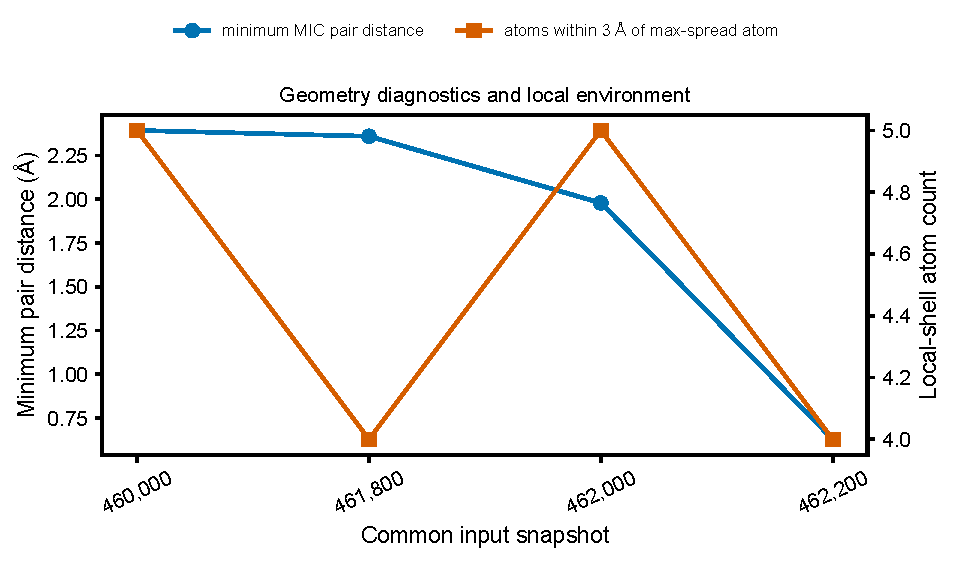
\includegraphics[width=\linewidth,height=0.42\textheight,keepaspectratio]{figure_pages/assets/fig_078.pdf}
\caption{Static force-disagreement and model-transfer diagnostics. This page shows the candidate output ``Fig3 geometry step diagnostics'' within the audited P1-FORCE family. The panel identity, source scope, and current status are retained in the accompanying evidence matrix.}
\label{fig:candidate_078}
\end{figure}
\textbf{Results text draft.} The figure compares model forces on a common set of configurations and exposes disagreement patterns that are not reducible to a single aggregate RMSE. The exact sampling scope and model provenance are retained in the evidence row.
\textbf{Discussion and boundary.} This supports the static-reference part of the benchmark. It does not by itself establish stability on a dynamically evolving path or agreement with converged DFT barriers.
\textbf{Article placement.} Proposed article location: Results: model disagreement and trajectory-integrity gate.
\textbf{Reviewer linkage:} overall status NO\_DIRECT\_REVIEWER\_FIGURE\_LINK.
No direct reviewer-response figure linkage was identified; this page is retained for scientific/article audit rather than as a direct reviewer response.
\textbf{Evidence pointers.}
\begin{itemize}[leftmargin=1.4em,noitemsep]
\item Data/processed: \begingroup\scriptsize\url{ablation/analysis/phase1_static_force_comparison_20261002/models_rockfish.json}\endgroup
\item Caption/text source: \begingroup\scriptsize\url{ablation/analysis/phase1_static_force_comparison_20261002/Methods.md}\endgroup
\item Caption/text source: \begingroup\scriptsize\url{ablation/analysis/phase1_static_force_comparison_20261002/README.md}\endgroup
\end{itemize}
\statusline{\textbf{Audit gap / next action:} Not yet integrated into the paper source}
\vfill
\clearpage
\section{FIG-079 --- Handoff stability heatmap}
\label{figpage:fig-079}
\textbf{Group:} P2-HANDOFF\quad \textbf{Evidence chain:} traceable\quad \textbf{Status:} unclassified
\begin{figure}[H]
\centering
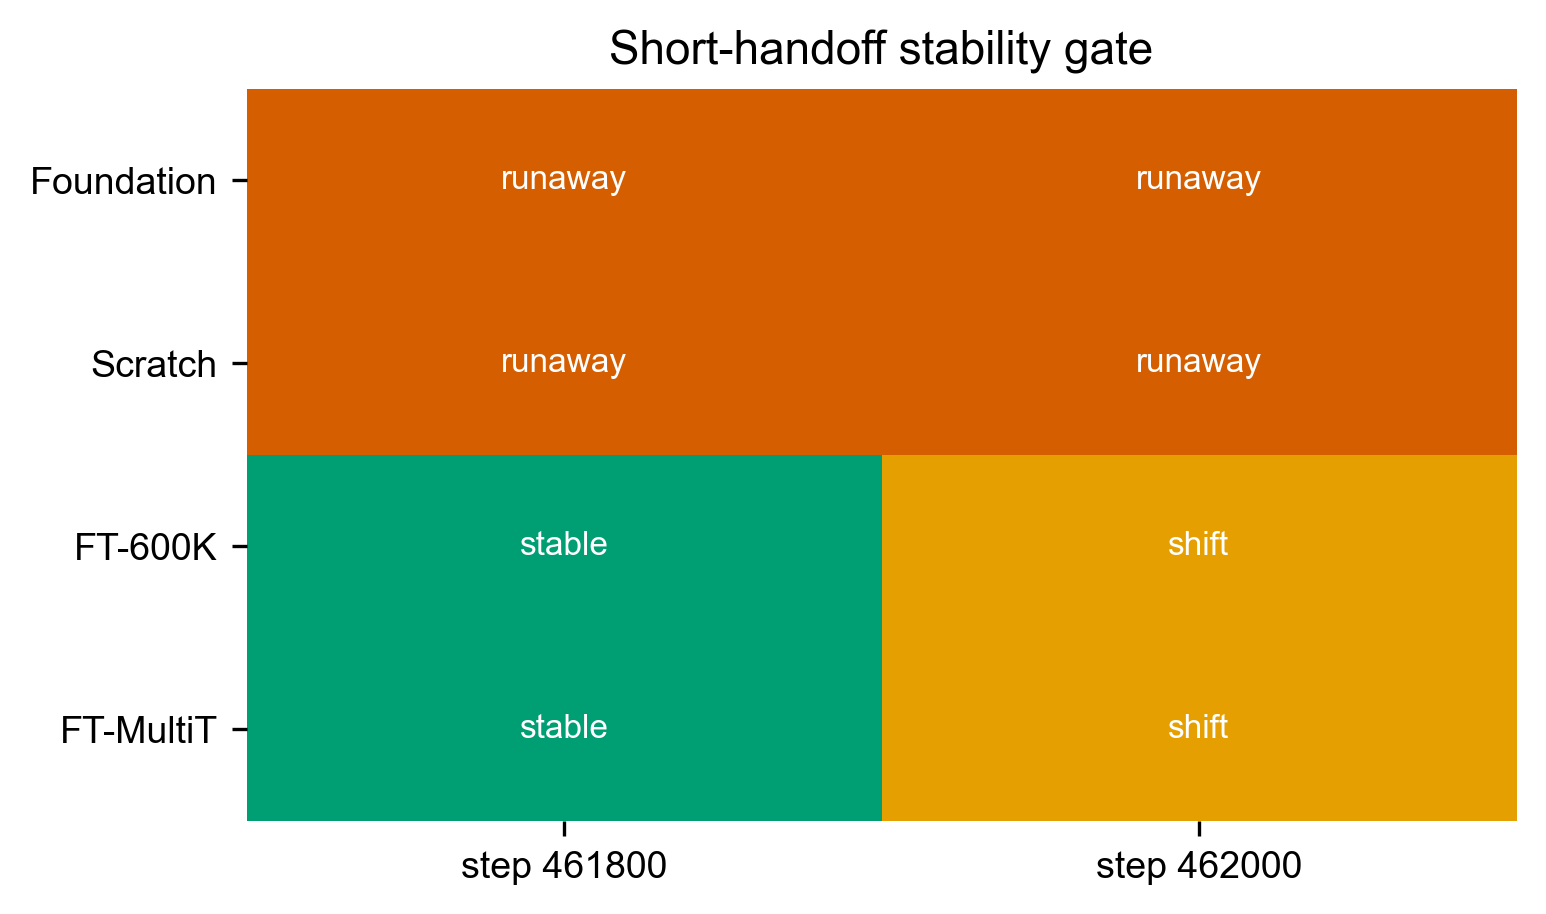
\includegraphics[width=\linewidth,height=0.42\textheight,keepaspectratio]{figure_pages/assets/fig_079.png}
\caption{Handoff molecular-dynamics diagnostics and first-divergence audit. This page shows the candidate output ``Handoff stability heatmap'' within the audited P2-HANDOFF family. The panel identity, source scope, and current status are retained in the accompanying evidence matrix.}
\label{fig:candidate_079}
\end{figure}
\textbf{Results text draft.} The panels track the temperature, force, contact, and structural observables used to locate the first anomalous behavior after protocol handoff. Run-level integrity and local-neighborhood evidence are kept alongside the visualization.
\textbf{Discussion and boundary.} This is a diagnostic figure for identifying when and how trajectories depart from the accepted regime. It is not a replacement for a completed, gate-passing production trajectory.
\textbf{Article placement.} Proposed article location: Results: dynamic stability mechanism; possibly SI.
\textbf{Reviewer linkage:} overall status NO\_DIRECT\_REVIEWER\_FIGURE\_LINK.
No direct reviewer-response figure linkage was identified; this page is retained for scientific/article audit rather than as a direct reviewer response.
\textbf{Evidence pointers.}
\begin{itemize}[leftmargin=1.4em,noitemsep]
\item Data/processed: \begingroup\scriptsize\url{ablation/analysis/phase2_handoff_md_20261002/remote_artifacts/runs/retry2/stability_summary.csv}\endgroup
\item Data/processed: \begingroup\scriptsize\url{ablation/analysis/phase2_handoff_md_20261002/remote_artifacts/runs/retry2/stability_summary.json}\endgroup
\end{itemize}
\statusline{\textbf{Audit gap / next action:} Keep duplicate retry/audit renders linked and designate one canonical output}
\vfill
\clearpage
\section{FIG-080 --- Handoff timeseries}
\label{figpage:fig-080}
\textbf{Group:} P2-HANDOFF\quad \textbf{Evidence chain:} traceable\quad \textbf{Status:} unclassified
\begin{figure}[H]
\centering
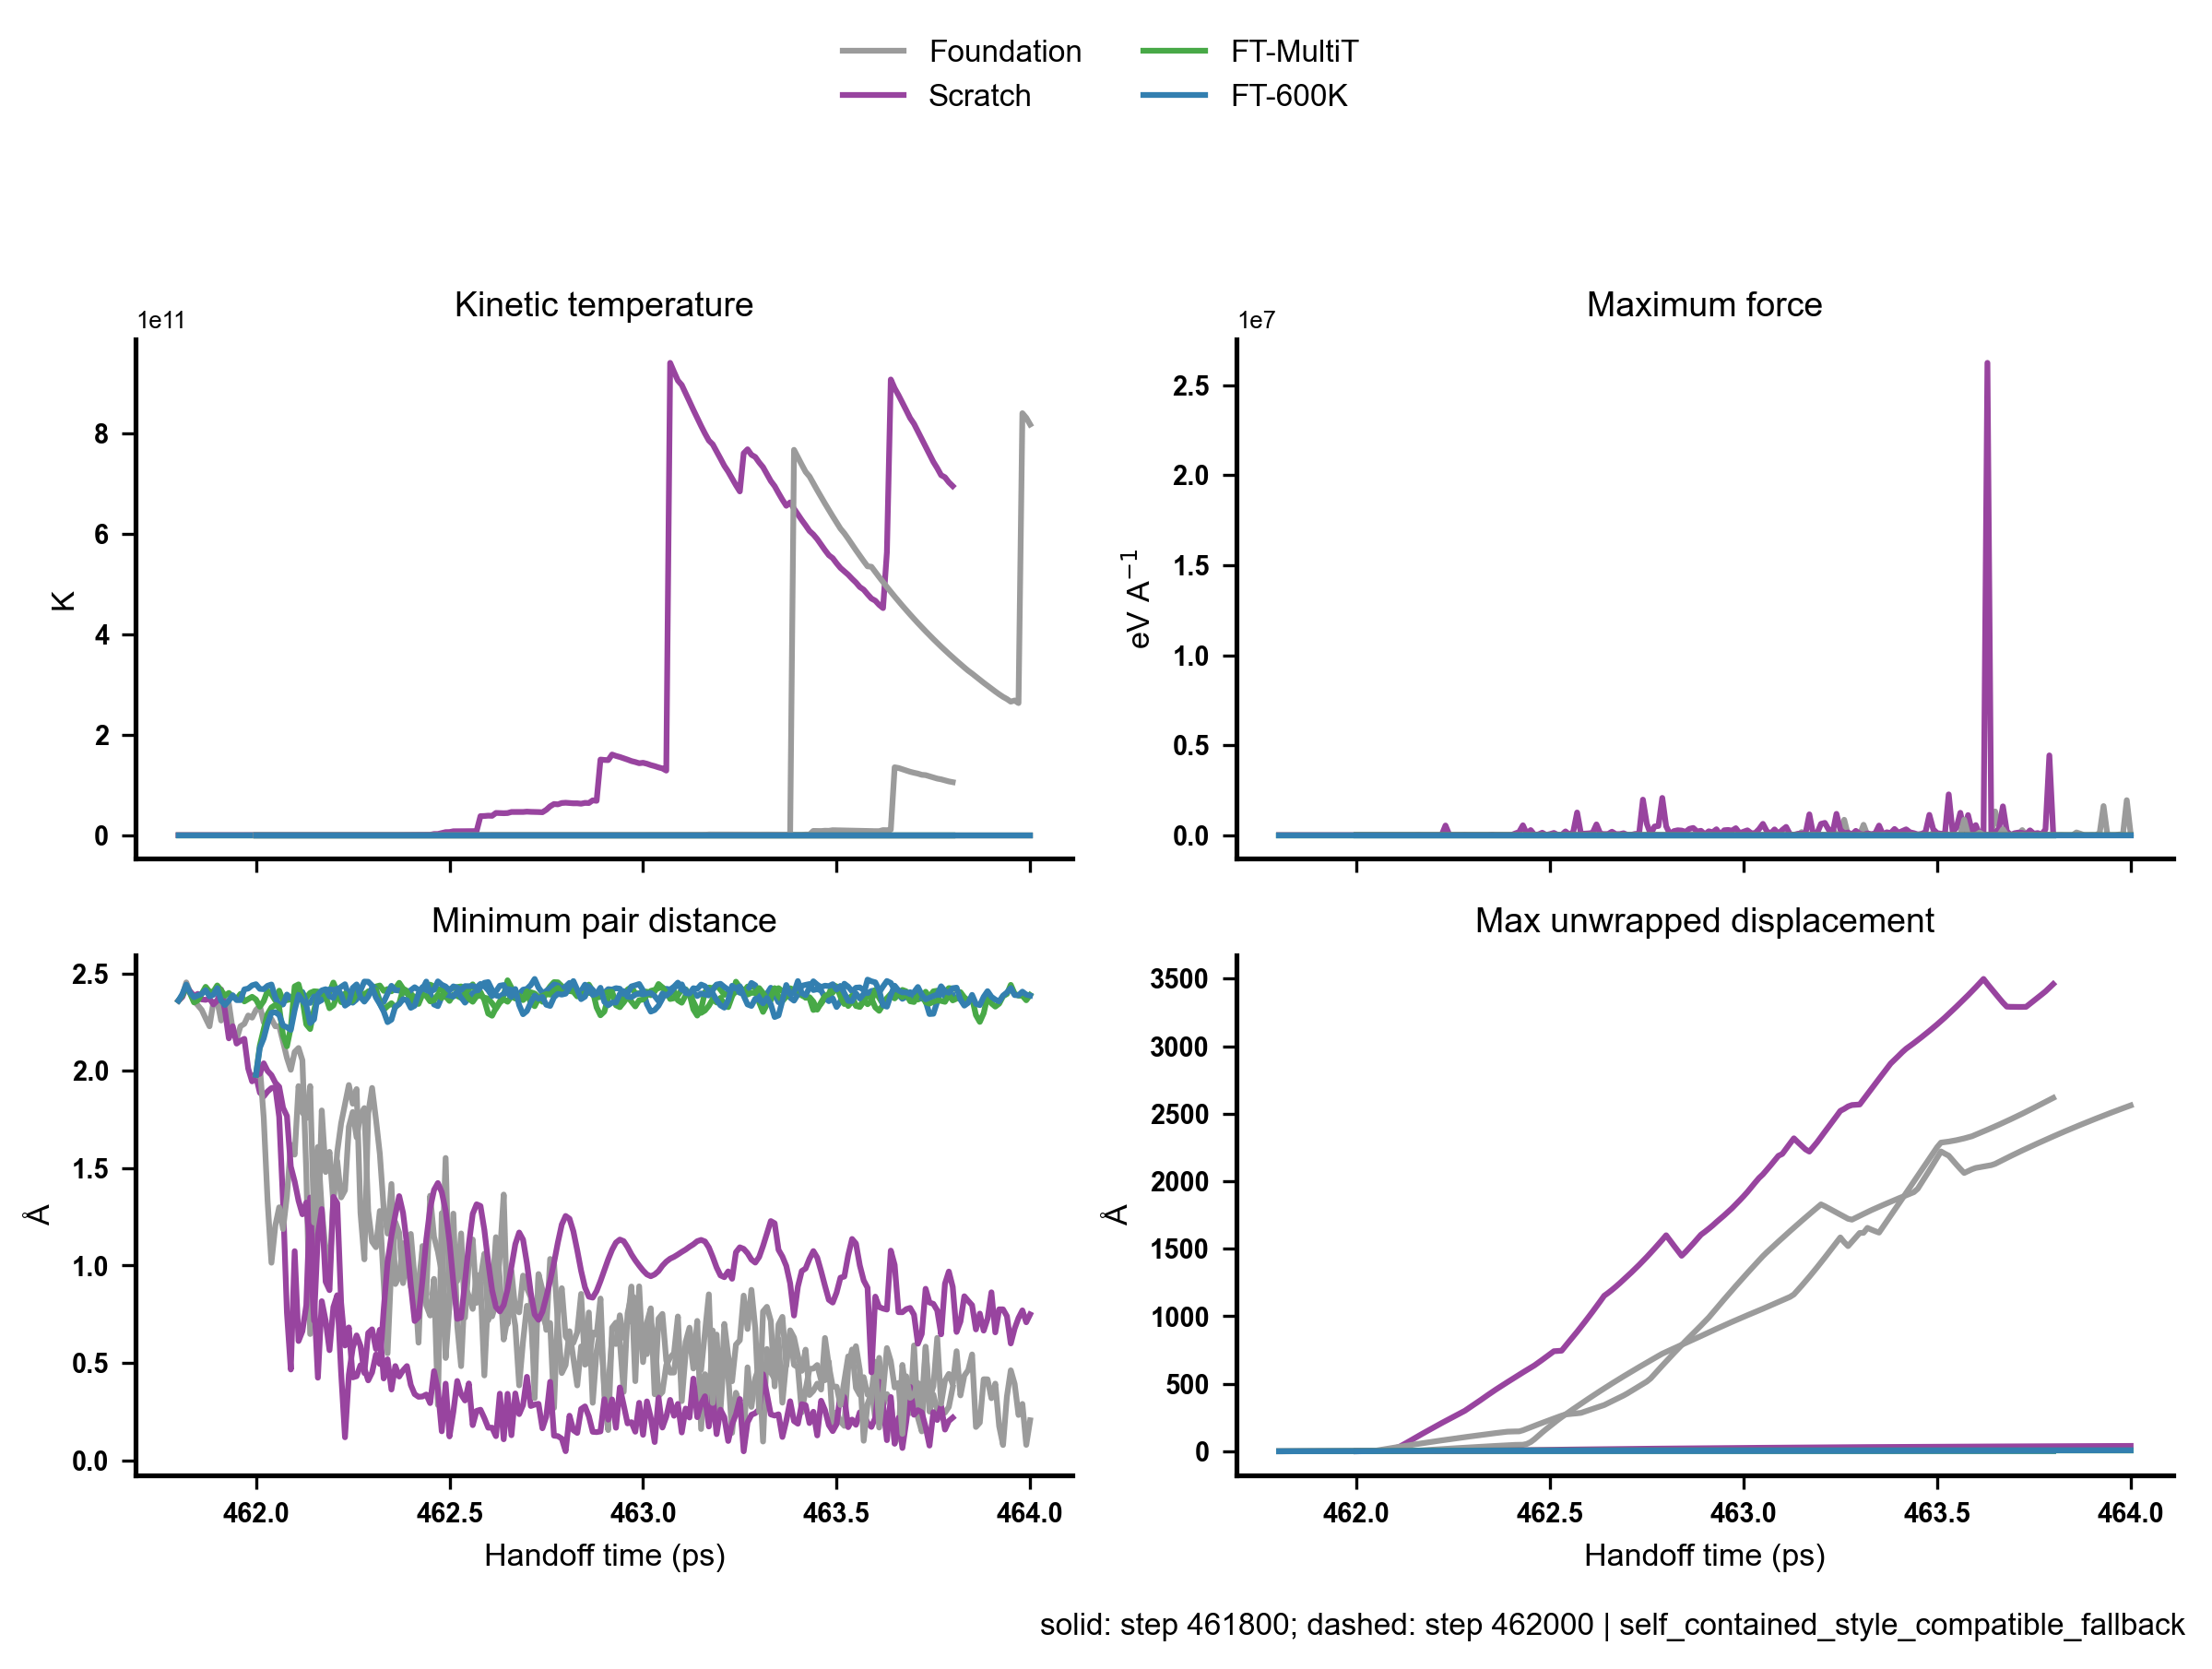
\includegraphics[width=\linewidth,height=0.42\textheight,keepaspectratio]{figure_pages/assets/fig_080.png}
\caption{Handoff molecular-dynamics diagnostics and first-divergence audit. This page shows the candidate output ``Handoff timeseries'' within the audited P2-HANDOFF family. The panel identity, source scope, and current status are retained in the accompanying evidence matrix.}
\label{fig:candidate_080}
\end{figure}
\textbf{Results text draft.} The panels track the temperature, force, contact, and structural observables used to locate the first anomalous behavior after protocol handoff. Run-level integrity and local-neighborhood evidence are kept alongside the visualization.
\textbf{Discussion and boundary.} This is a diagnostic figure for identifying when and how trajectories depart from the accepted regime. It is not a replacement for a completed, gate-passing production trajectory.
\textbf{Article placement.} Proposed article location: Results: dynamic stability mechanism; possibly SI.
\textbf{Reviewer linkage:} overall status NO\_DIRECT\_REVIEWER\_FIGURE\_LINK.
No direct reviewer-response figure linkage was identified; this page is retained for scientific/article audit rather than as a direct reviewer response.
\textbf{Evidence pointers.}
\begin{itemize}[leftmargin=1.4em,noitemsep]
\item Data/processed: \begingroup\scriptsize\url{ablation/analysis/phase2_handoff_md_20261002/remote_artifacts/runs/retry2/stability_summary.csv}\endgroup
\item Data/processed: \begingroup\scriptsize\url{ablation/analysis/phase2_handoff_md_20261002/remote_artifacts/runs/retry2/stability_summary.json}\endgroup
\end{itemize}
\statusline{\textbf{Audit gap / next action:} Keep duplicate retry/audit renders linked and designate one canonical output}
\vfill
\clearpage
\section{FIG-081 --- Placeholder dft gate status}
\label{figpage:fig-081}
\textbf{Group:} TASK2-ROSTER\quad \textbf{Evidence chain:} traceable\quad \textbf{Status:} placeholder
\begin{figure}[H]
\centering
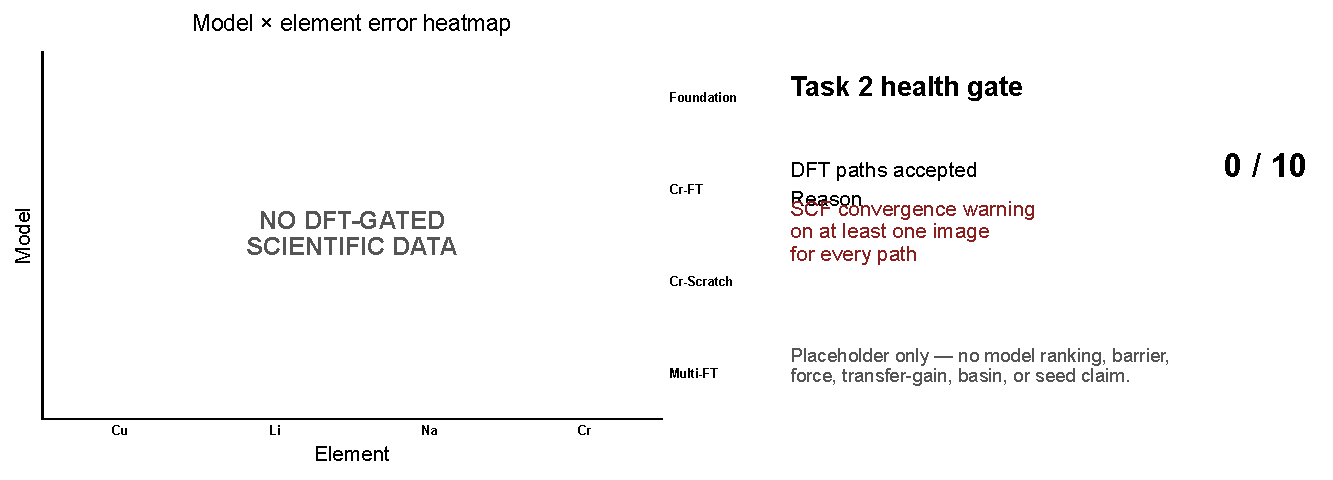
\includegraphics[width=\linewidth,height=0.42\textheight,keepaspectratio]{figure_pages/assets/fig_081.pdf}
\caption{Cross-element or multi-seed benchmark roster and pathway diagnostics. This page shows the candidate output ``Placeholder dft gate status'' within the audited TASK2-ROSTER family. The panel identity, source scope, and current status are retained in the accompanying evidence matrix.}
\label{fig:candidate_081}
\end{figure}
\textbf{Results text draft.} The figure organizes the evaluated systems, seeds, models, or pathway families so that coverage and missing cells are visible. Provisional and audited rows are not pooled when their protocols or provenance differ.
\textbf{Discussion and boundary.} This is appropriate for SI coverage and provenance discussion. It should not be read as a single uncertainty distribution across model-level and path-level variation.
\textbf{Article placement.} Proposed article location: Results: cross-element transfer and seed stability.
\textbf{Reviewer linkage:} overall status NO\_DIRECT\_REVIEWER\_FIGURE\_LINK.
No direct reviewer-response figure linkage was identified; this page is retained for scientific/article audit rather than as a direct reviewer response.
\textbf{Evidence pointers.}
\begin{itemize}[leftmargin=1.4em,noitemsep]
\item Caption/text source: \begingroup\scriptsize\url{ablation/analysis/task2_cross_element/HEALTH_GATE_REPORT.md}\endgroup
\end{itemize}
\statusline{\textbf{Audit gap / next action:} DFT gate is still open; do not write barrier-accuracy claims}
\vfill
\clearpage
\section{FIG-082 --- Endpoint initialization smoke}
\label{figpage:fig-082}
\textbf{Group:} TASK3-NEB\quad \textbf{Evidence chain:} partial\quad \textbf{Status:} unclassified
\begin{figure}[H]
\centering
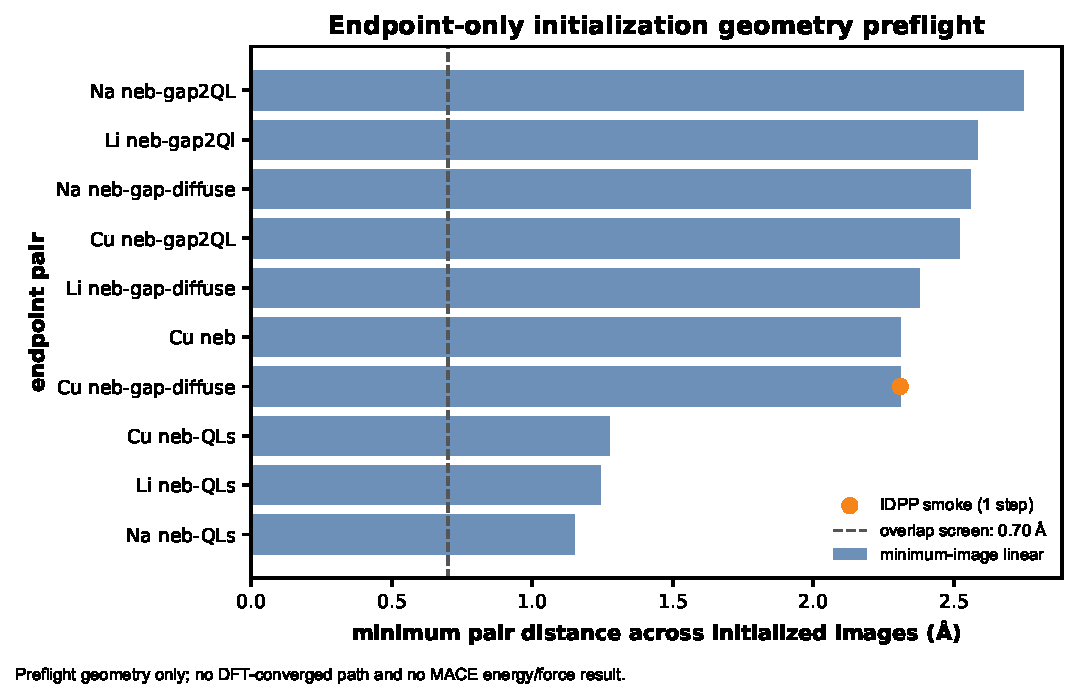
\includegraphics[width=\linewidth,height=0.42\textheight,keepaspectratio]{figure_pages/assets/fig_082.pdf}
\caption{Neb pathway, barrier, topology, or self-consistency diagnostics. This page shows the candidate output ``Endpoint initialization smoke'' within the audited TASK3-NEB family. The panel identity, source scope, and current status are retained in the accompanying evidence matrix.}
\label{fig:candidate_082}
\end{figure}
\textbf{Results text draft.} The panels distinguish fixed-path scoring, self-consistent MLFF-NEB behavior, endpoint/path topology checks, and DFT convergence status. These operators answer different questions and are kept separate in the text.
\textbf{Discussion and boundary.} A model-reported self-relaxed barrier must not be presented as the fixed-path DFT error, and a provisional or unconverged DFT path must not be promoted to a final reference barrier.
\textbf{Article placement.} Proposed article location: Results or SI: path-family diagnostics.
\textbf{Reviewer linkage:} overall status PARTIAL.
\begin{itemize}[leftmargin=1.4em,noitemsep]
\item \textbf{REV-A1 (PARTIAL):} Reconcile Fig. 3d fixed-geometry DFT-path scoring with SI Fig. S3 self-consistent MLFF-NEB, including pathway identity and the DFT reference. \emph{Completed:} The fixed-path versus self-relaxed operator distinction and the narrower model-reported-barrier wording are integrated. \emph{Still required:} Close the restartable QE path-1--4 convergence gate, preserve the final path/source metadata, and complete the SI Fig. S3 endpoint/checkpoint/optimizer/source audit before calling the quantitative reference final.
\end{itemize}
\textbf{Evidence pointers.}
\begin{itemize}[leftmargin=1.4em,noitemsep]
\item Data/processed: \begingroup\scriptsize\url{ablation/analysis/task3_endpoint_only_neb/dft_gate_manifest.csv}\endgroup
\item Data/processed: \begingroup\scriptsize\url{ablation/analysis/task3_endpoint_only_neb/endpoint_only_leakage_audit.csv}\endgroup
\item Plot/processing script: \begingroup\scriptsize\url{ablation/analysis/task3_endpoint_only_neb/analyze_all_foundation_models.py}\endgroup
\item Plot/processing script: \begingroup\scriptsize\url{ablation/analysis/task3_endpoint_only_neb/analyze_corrected_dft_foundation_comparison.py}\endgroup
\item Caption/text source: \begingroup\scriptsize\url{ablation/analysis/task3_endpoint_only_neb/README.md}\endgroup
\end{itemize}
\statusline{\textbf{Audit gap / next action:} Many per-path exports have no co-located generator; use the parent renderer and record the exact input tables}
\vfill
\clearpage
\section{FIG-083 --- Figure corrected dft foundation barrier comparison}
\label{figpage:fig-083}
\textbf{Group:} TASK3-NEB\quad \textbf{Evidence chain:} partial\quad \textbf{Status:} exploratory;audit;comparison
\begin{figure}[H]
\centering
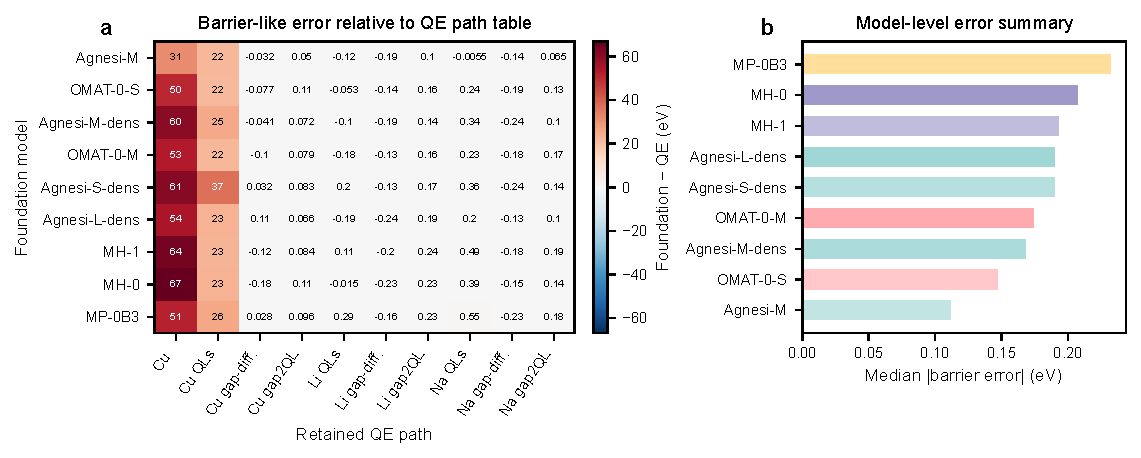
\includegraphics[width=\linewidth,height=0.42\textheight,keepaspectratio]{figure_pages/assets/fig_083.pdf}
\caption{Neb pathway, barrier, topology, or self-consistency diagnostics. This page shows the candidate output ``Figure corrected dft foundation barrier comparison'' within the audited TASK3-NEB family. The panel identity, source scope, and current status are retained in the accompanying evidence matrix.}
\label{fig:candidate_083}
\end{figure}
\textbf{Results text draft.} The panels distinguish fixed-path scoring, self-consistent MLFF-NEB behavior, endpoint/path topology checks, and DFT convergence status. These operators answer different questions and are kept separate in the text.
\textbf{Discussion and boundary.} A model-reported self-relaxed barrier must not be presented as the fixed-path DFT error, and a provisional or unconverged DFT path must not be promoted to a final reference barrier.
\textbf{Article placement.} Proposed article location: Results or SI: path-family diagnostics.
\textbf{Reviewer linkage:} overall status PARTIAL.
\begin{itemize}[leftmargin=1.4em,noitemsep]
\item \textbf{REV-A1 (PARTIAL):} Reconcile Fig. 3d fixed-geometry DFT-path scoring with SI Fig. S3 self-consistent MLFF-NEB, including pathway identity and the DFT reference. \emph{Completed:} The fixed-path versus self-relaxed operator distinction and the narrower model-reported-barrier wording are integrated. \emph{Still required:} Close the restartable QE path-1--4 convergence gate, preserve the final path/source metadata, and complete the SI Fig. S3 endpoint/checkpoint/optimizer/source audit before calling the quantitative reference final.
\end{itemize}
\textbf{Evidence pointers.}
\begin{itemize}[leftmargin=1.4em,noitemsep]
\item Data/processed: \begingroup\scriptsize\url{ablation/analysis/task3_endpoint_only_neb/exploratory_energy_audit/all_dft_foundation_models/corrected_dft_foundation_image_profiles.csv}\endgroup
\item Data/processed: \begingroup\scriptsize\url{ablation/analysis/task3_endpoint_only_neb/exploratory_energy_audit/all_dft_foundation_models/corrected_dft_foundation_manifest.json}\endgroup
\item Plot/processing script: \begingroup\scriptsize\url{ablation/analysis/task3_endpoint_only_neb/exploratory_energy_audit/plot_paper_figures.py}\endgroup
\item Caption/text source: \begingroup\scriptsize\url{ablation/analysis/task3_endpoint_only_neb/exploratory_energy_audit/ACCEPTANCE_MATRIX.md}\endgroup
\item Caption/text source: \begingroup\scriptsize\url{ablation/analysis/task3_endpoint_only_neb/exploratory_energy_audit/EXPLORATORY_REPORT.md}\endgroup
\end{itemize}
\statusline{\textbf{Audit gap / next action:} Many per-path exports have no co-located generator; use the parent renderer and record the exact input tables}
\vfill
\clearpage
\section{FIG-084 --- Figure corrected dft foundation path profiles}
\label{figpage:fig-084}
\textbf{Group:} TASK3-NEB\quad \textbf{Evidence chain:} partial\quad \textbf{Status:} exploratory;audit;comparison
\begin{figure}[H]
\centering
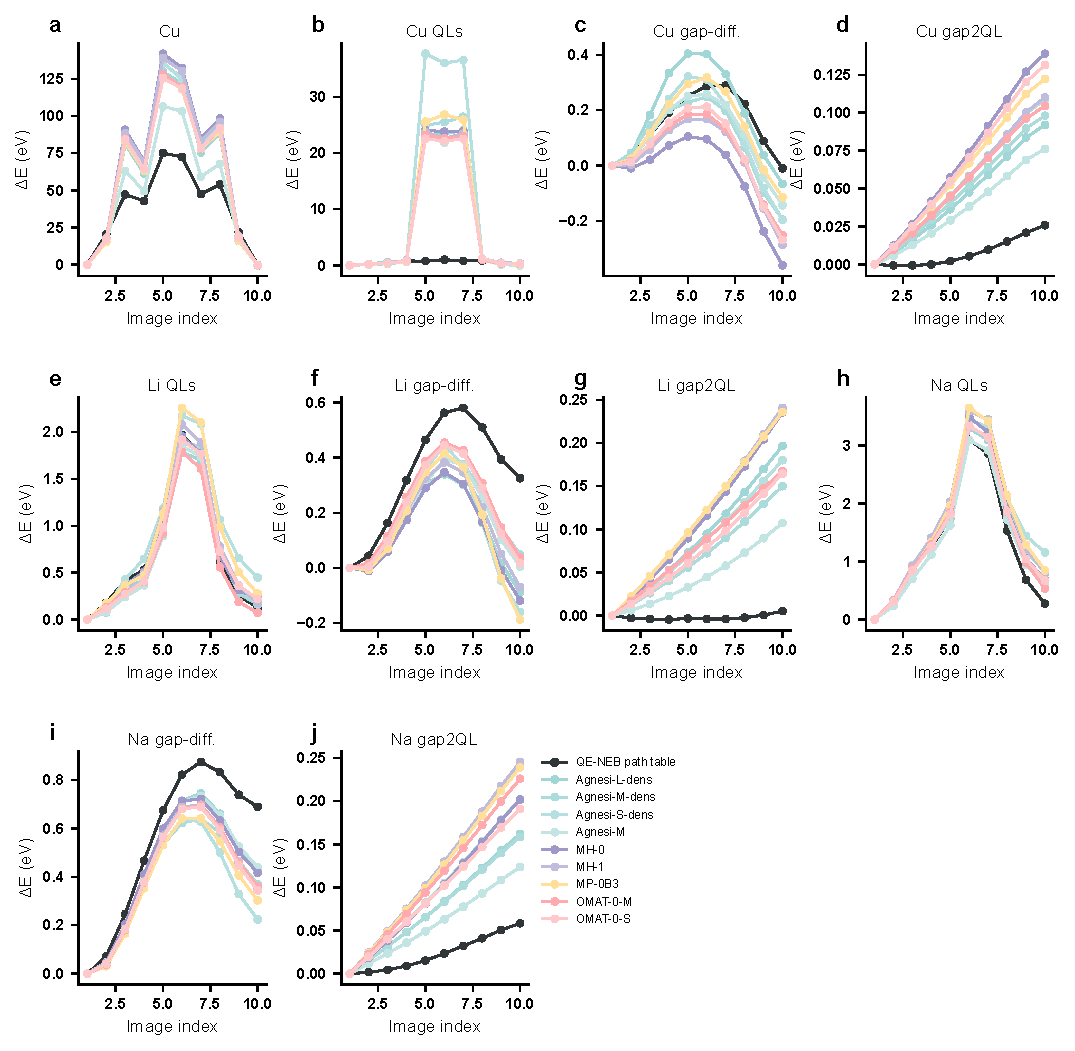
\includegraphics[width=\linewidth,height=0.42\textheight,keepaspectratio]{figure_pages/assets/fig_084.pdf}
\caption{Neb pathway, barrier, topology, or self-consistency diagnostics. This page shows the candidate output ``Figure corrected dft foundation path profiles'' within the audited TASK3-NEB family. The panel identity, source scope, and current status are retained in the accompanying evidence matrix.}
\label{fig:candidate_084}
\end{figure}
\textbf{Results text draft.} The panels distinguish fixed-path scoring, self-consistent MLFF-NEB behavior, endpoint/path topology checks, and DFT convergence status. These operators answer different questions and are kept separate in the text.
\textbf{Discussion and boundary.} A model-reported self-relaxed barrier must not be presented as the fixed-path DFT error, and a provisional or unconverged DFT path must not be promoted to a final reference barrier.
\textbf{Article placement.} Proposed article location: Results or SI: path-family diagnostics.
\textbf{Reviewer linkage:} overall status PARTIAL.
\begin{itemize}[leftmargin=1.4em,noitemsep]
\item \textbf{REV-A1 (PARTIAL):} Reconcile Fig. 3d fixed-geometry DFT-path scoring with SI Fig. S3 self-consistent MLFF-NEB, including pathway identity and the DFT reference. \emph{Completed:} The fixed-path versus self-relaxed operator distinction and the narrower model-reported-barrier wording are integrated. \emph{Still required:} Close the restartable QE path-1--4 convergence gate, preserve the final path/source metadata, and complete the SI Fig. S3 endpoint/checkpoint/optimizer/source audit before calling the quantitative reference final.
\end{itemize}
\textbf{Evidence pointers.}
\begin{itemize}[leftmargin=1.4em,noitemsep]
\item Data/processed: \begingroup\scriptsize\url{ablation/analysis/task3_endpoint_only_neb/exploratory_energy_audit/all_dft_foundation_models/corrected_dft_foundation_image_profiles.csv}\endgroup
\item Data/processed: \begingroup\scriptsize\url{ablation/analysis/task3_endpoint_only_neb/exploratory_energy_audit/all_dft_foundation_models/corrected_dft_foundation_manifest.json}\endgroup
\item Plot/processing script: \begingroup\scriptsize\url{ablation/analysis/task3_endpoint_only_neb/exploratory_energy_audit/plot_paper_figures.py}\endgroup
\item Caption/text source: \begingroup\scriptsize\url{ablation/analysis/task3_endpoint_only_neb/exploratory_energy_audit/ACCEPTANCE_MATRIX.md}\endgroup
\item Caption/text source: \begingroup\scriptsize\url{ablation/analysis/task3_endpoint_only_neb/exploratory_energy_audit/EXPLORATORY_REPORT.md}\endgroup
\end{itemize}
\statusline{\textbf{Audit gap / next action:} Many per-path exports have no co-located generator; use the parent renderer and record the exact input tables}
\vfill
\clearpage
\section{FIG-085 --- Figure diagnostic framework overview}
\label{figpage:fig-085}
\textbf{Group:} TASK3-NEB\quad \textbf{Evidence chain:} partial\quad \textbf{Status:} exploratory;audit
\begin{figure}[H]
\centering
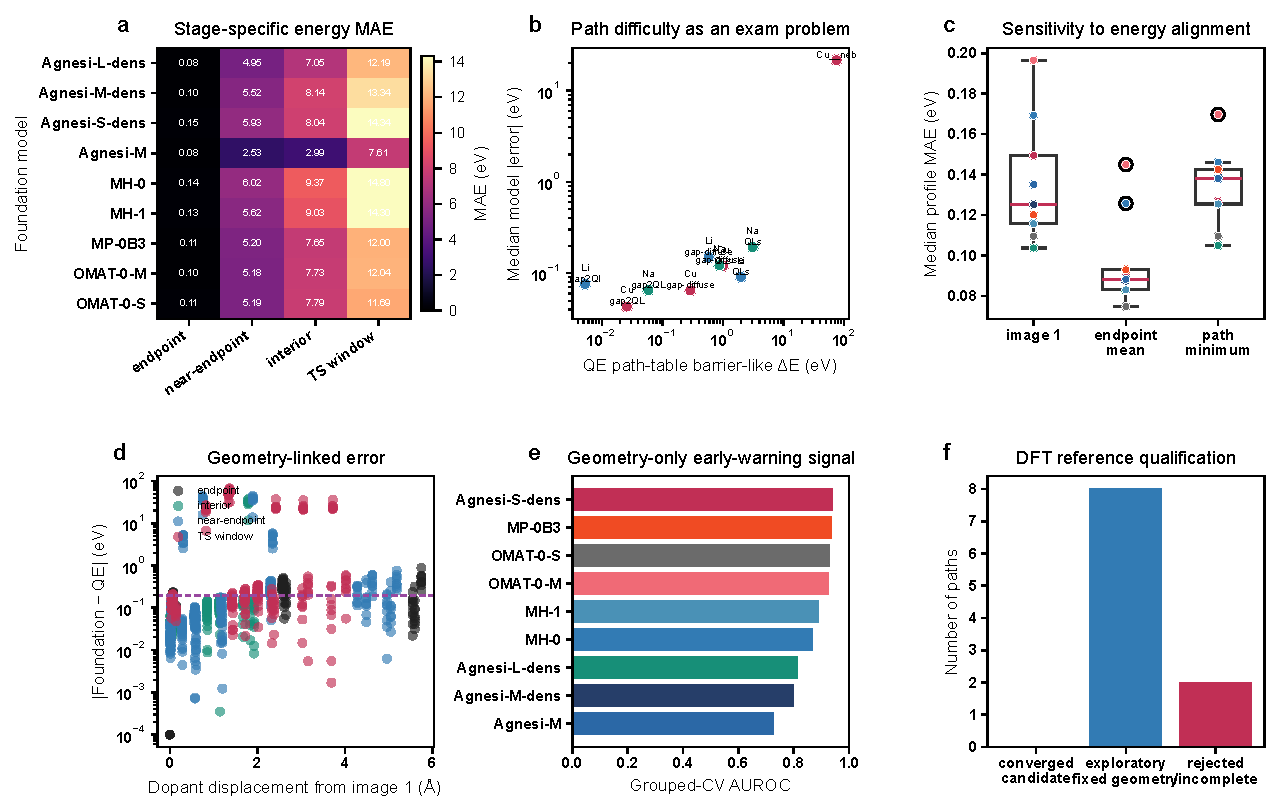
\includegraphics[width=\linewidth,height=0.42\textheight,keepaspectratio]{figure_pages/assets/fig_085.pdf}
\caption{Neb pathway, barrier, topology, or self-consistency diagnostics. This page shows the candidate output ``Figure diagnostic framework overview'' within the audited TASK3-NEB family. The panel identity, source scope, and current status are retained in the accompanying evidence matrix.}
\label{fig:candidate_085}
\end{figure}
\textbf{Results text draft.} The panels distinguish fixed-path scoring, self-consistent MLFF-NEB behavior, endpoint/path topology checks, and DFT convergence status. These operators answer different questions and are kept separate in the text.
\textbf{Discussion and boundary.} A model-reported self-relaxed barrier must not be presented as the fixed-path DFT error, and a provisional or unconverged DFT path must not be promoted to a final reference barrier.
\textbf{Article placement.} Proposed article location: Results or SI: path-family diagnostics.
\textbf{Reviewer linkage:} overall status PARTIAL.
\begin{itemize}[leftmargin=1.4em,noitemsep]
\item \textbf{REV-A1 (PARTIAL):} Reconcile Fig. 3d fixed-geometry DFT-path scoring with SI Fig. S3 self-consistent MLFF-NEB, including pathway identity and the DFT reference. \emph{Completed:} The fixed-path versus self-relaxed operator distinction and the narrower model-reported-barrier wording are integrated. \emph{Still required:} Close the restartable QE path-1--4 convergence gate, preserve the final path/source metadata, and complete the SI Fig. S3 endpoint/checkpoint/optimizer/source audit before calling the quantitative reference final.
\end{itemize}
\textbf{Evidence pointers.}
\begin{itemize}[leftmargin=1.4em,noitemsep]
\item Data/processed: \begingroup\scriptsize\url{ablation/analysis/task3_endpoint_only_neb/exploratory_energy_audit/all_path_diagnostic_framework/alignment_profile_errors.csv}\endgroup
\item Data/processed: \begingroup\scriptsize\url{ablation/analysis/task3_endpoint_only_neb/exploratory_energy_audit/all_path_diagnostic_framework/alignment_sensitivity_summary.csv}\endgroup
\item Plot/processing script: \begingroup\scriptsize\url{ablation/analysis/task3_endpoint_only_neb/exploratory_energy_audit/plot_paper_figures.py}\endgroup
\item Caption/text source: \begingroup\scriptsize\url{ablation/analysis/task3_endpoint_only_neb/exploratory_energy_audit/ACCEPTANCE_MATRIX.md}\endgroup
\item Caption/text source: \begingroup\scriptsize\url{ablation/analysis/task3_endpoint_only_neb/exploratory_energy_audit/EXPLORATORY_REPORT.md}\endgroup
\end{itemize}
\statusline{\textbf{Audit gap / next action:} Many per-path exports have no co-located generator; use the parent renderer and record the exact input tables}
\vfill
\clearpage
\section{FIG-086 --- Figure path type summary}
\label{figpage:fig-086}
\textbf{Group:} TASK3-NEB\quad \textbf{Evidence chain:} partial\quad \textbf{Status:} exploratory;audit
\begin{figure}[H]
\centering
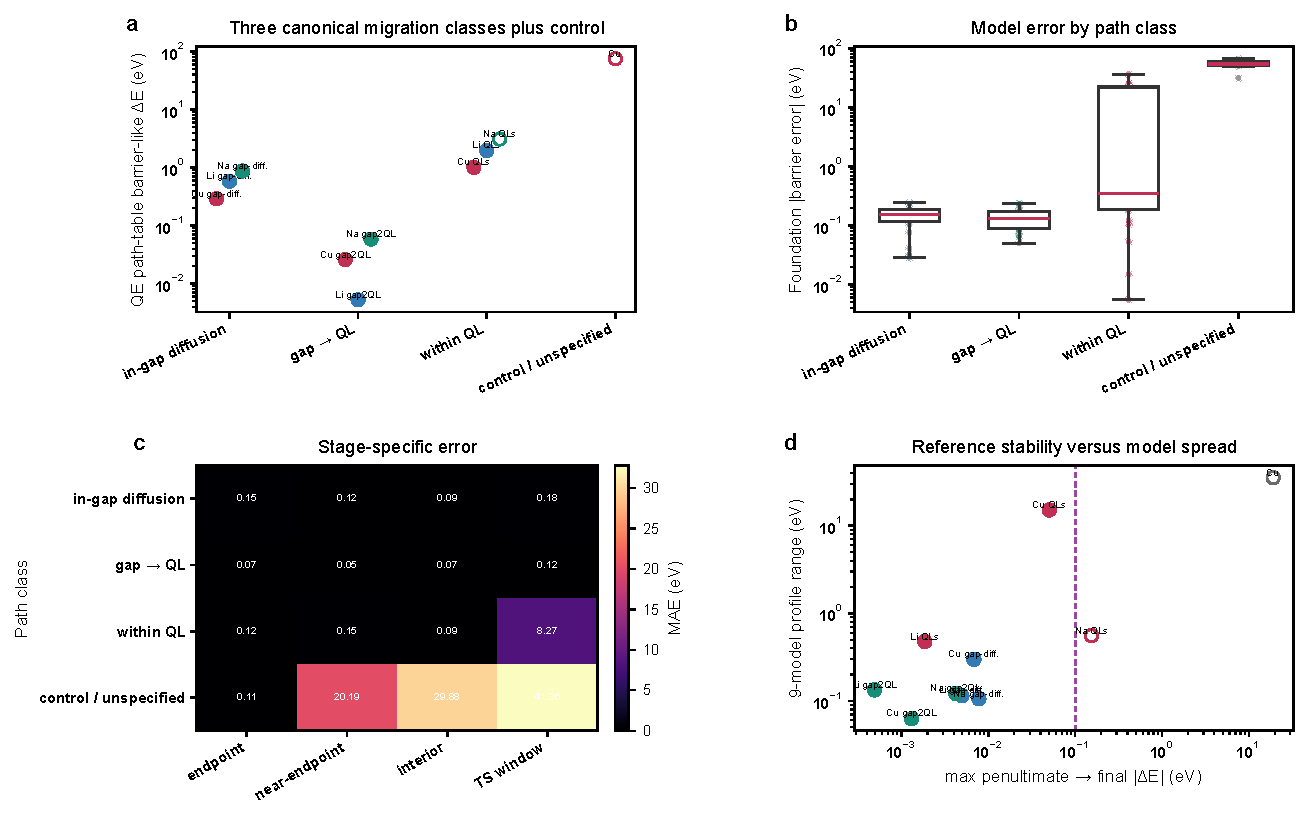
\includegraphics[width=\linewidth,height=0.42\textheight,keepaspectratio]{figure_pages/assets/fig_086.pdf}
\caption{Neb pathway, barrier, topology, or self-consistency diagnostics. This page shows the candidate output ``Figure path type summary'' within the audited TASK3-NEB family. The panel identity, source scope, and current status are retained in the accompanying evidence matrix.}
\label{fig:candidate_086}
\end{figure}
\textbf{Results text draft.} The panels distinguish fixed-path scoring, self-consistent MLFF-NEB behavior, endpoint/path topology checks, and DFT convergence status. These operators answer different questions and are kept separate in the text.
\textbf{Discussion and boundary.} A model-reported self-relaxed barrier must not be presented as the fixed-path DFT error, and a provisional or unconverged DFT path must not be promoted to a final reference barrier.
\textbf{Article placement.} Proposed article location: Results or SI: path-family diagnostics.
\textbf{Reviewer linkage:} overall status PARTIAL.
\begin{itemize}[leftmargin=1.4em,noitemsep]
\item \textbf{REV-A1 (PARTIAL):} Reconcile Fig. 3d fixed-geometry DFT-path scoring with SI Fig. S3 self-consistent MLFF-NEB, including pathway identity and the DFT reference. \emph{Completed:} The fixed-path versus self-relaxed operator distinction and the narrower model-reported-barrier wording are integrated. \emph{Still required:} Close the restartable QE path-1--4 convergence gate, preserve the final path/source metadata, and complete the SI Fig. S3 endpoint/checkpoint/optimizer/source audit before calling the quantitative reference final.
\end{itemize}
\textbf{Evidence pointers.}
\begin{itemize}[leftmargin=1.4em,noitemsep]
\item Data/processed: \begingroup\scriptsize\url{ablation/analysis/task3_endpoint_only_neb/exploratory_energy_audit/all_path_diagnostic_framework/alignment_profile_errors.csv}\endgroup
\item Data/processed: \begingroup\scriptsize\url{ablation/analysis/task3_endpoint_only_neb/exploratory_energy_audit/all_path_diagnostic_framework/alignment_sensitivity_summary.csv}\endgroup
\item Plot/processing script: \begingroup\scriptsize\url{ablation/analysis/task3_endpoint_only_neb/exploratory_energy_audit/plot_paper_figures.py}\endgroup
\item Caption/text source: \begingroup\scriptsize\url{ablation/analysis/task3_endpoint_only_neb/exploratory_energy_audit/ACCEPTANCE_MATRIX.md}\endgroup
\item Caption/text source: \begingroup\scriptsize\url{ablation/analysis/task3_endpoint_only_neb/exploratory_energy_audit/EXPLORATORY_REPORT.md}\endgroup
\end{itemize}
\statusline{\textbf{Audit gap / next action:} Many per-path exports have no co-located generator; use the parent renderer and record the exact input tables}
\vfill
\clearpage
\section{FIG-087 --- Figure structural stage diagnostics}
\label{figpage:fig-087}
\textbf{Group:} TASK3-NEB\quad \textbf{Evidence chain:} partial\quad \textbf{Status:} exploratory;audit
\begin{figure}[H]
\centering
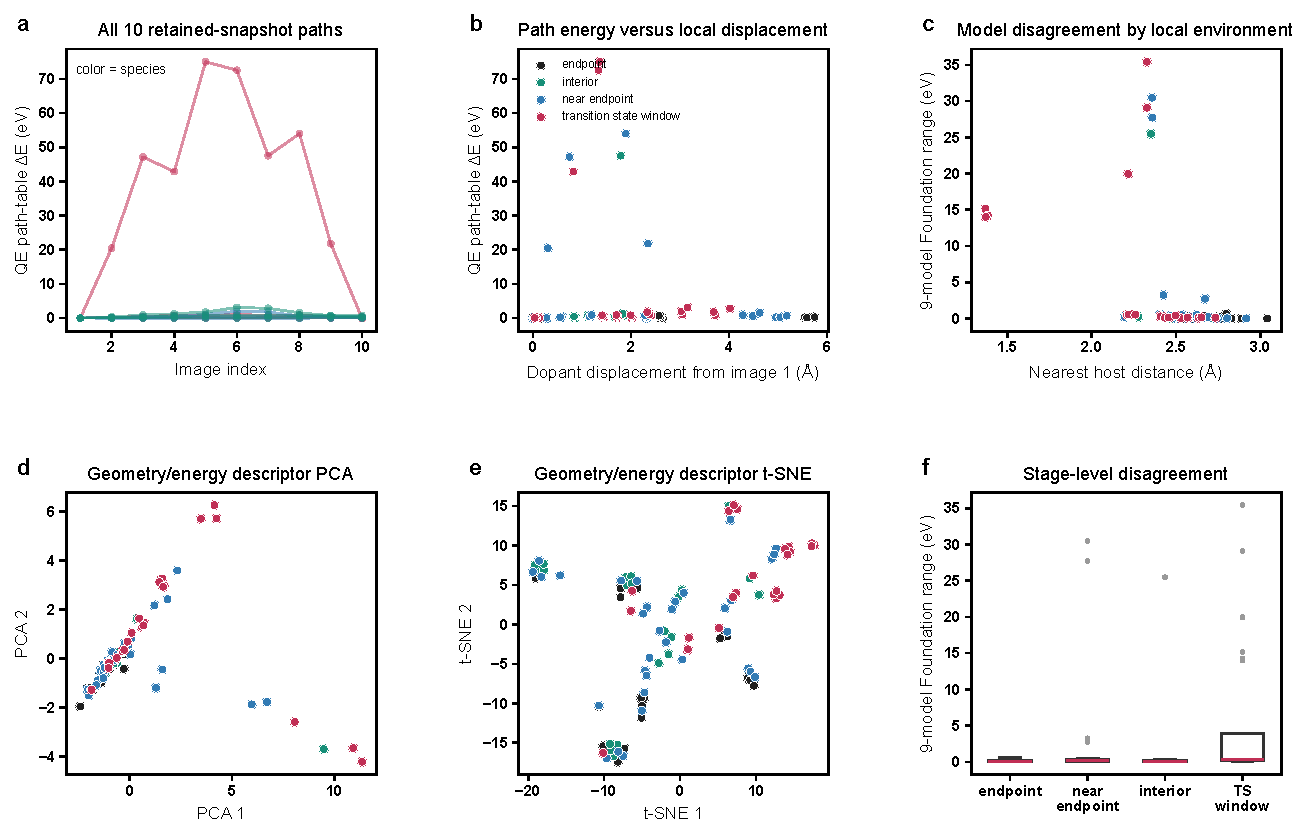
\includegraphics[width=\linewidth,height=0.42\textheight,keepaspectratio]{figure_pages/assets/fig_087.pdf}
\caption{Neb pathway, barrier, topology, or self-consistency diagnostics. This page shows the candidate output ``Figure structural stage diagnostics'' within the audited TASK3-NEB family. The panel identity, source scope, and current status are retained in the accompanying evidence matrix.}
\label{fig:candidate_087}
\end{figure}
\textbf{Results text draft.} The panels distinguish fixed-path scoring, self-consistent MLFF-NEB behavior, endpoint/path topology checks, and DFT convergence status. These operators answer different questions and are kept separate in the text.
\textbf{Discussion and boundary.} A model-reported self-relaxed barrier must not be presented as the fixed-path DFT error, and a provisional or unconverged DFT path must not be promoted to a final reference barrier.
\textbf{Article placement.} Proposed article location: Results or SI: path-family diagnostics.
\textbf{Reviewer linkage:} overall status PARTIAL.
\begin{itemize}[leftmargin=1.4em,noitemsep]
\item \textbf{REV-A1 (PARTIAL):} Reconcile Fig. 3d fixed-geometry DFT-path scoring with SI Fig. S3 self-consistent MLFF-NEB, including pathway identity and the DFT reference. \emph{Completed:} The fixed-path versus self-relaxed operator distinction and the narrower model-reported-barrier wording are integrated. \emph{Still required:} Close the restartable QE path-1--4 convergence gate, preserve the final path/source metadata, and complete the SI Fig. S3 endpoint/checkpoint/optimizer/source audit before calling the quantitative reference final.
\end{itemize}
\textbf{Evidence pointers.}
\begin{itemize}[leftmargin=1.4em,noitemsep]
\item Data/processed: \begingroup\scriptsize\url{ablation/analysis/task3_endpoint_only_neb/exploratory_energy_audit/all_path_structural_diagnostics/neb_descriptor_embedding.csv}\endgroup
\item Data/processed: \begingroup\scriptsize\url{ablation/analysis/task3_endpoint_only_neb/exploratory_energy_audit/all_path_structural_diagnostics/qe_path_stage_summary.csv}\endgroup
\item Plot/processing script: \begingroup\scriptsize\url{ablation/analysis/task3_endpoint_only_neb/exploratory_energy_audit/plot_paper_figures.py}\endgroup
\item Caption/text source: \begingroup\scriptsize\url{ablation/analysis/task3_endpoint_only_neb/exploratory_energy_audit/ACCEPTANCE_MATRIX.md}\endgroup
\item Caption/text source: \begingroup\scriptsize\url{ablation/analysis/task3_endpoint_only_neb/exploratory_energy_audit/EXPLORATORY_REPORT.md}\endgroup
\end{itemize}
\statusline{\textbf{Audit gap / next action:} Many per-path exports have no co-located generator; use the parent renderer and record the exact input tables}
\vfill
\clearpage
\section{FIG-088 --- Figure corrected dft foundation barrier comparison}
\label{figpage:fig-088}
\textbf{Group:} TASK3-NEB\quad \textbf{Evidence chain:} partial\quad \textbf{Status:} exploratory;audit;comparison
\begin{figure}[H]
\centering
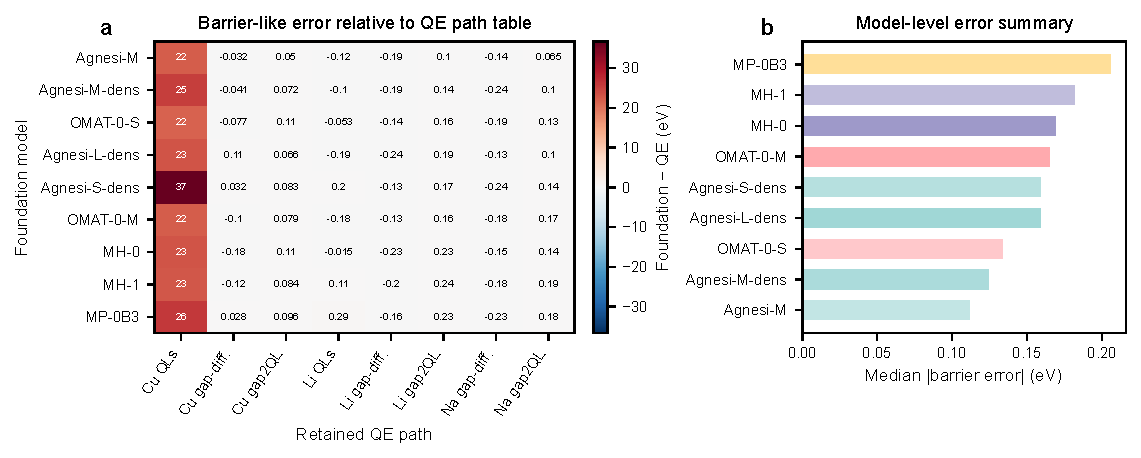
\includegraphics[width=\linewidth,height=0.42\textheight,keepaspectratio]{figure_pages/assets/fig_088.pdf}
\caption{Neb pathway, barrier, topology, or self-consistency diagnostics. This page shows the candidate output ``Figure corrected dft foundation barrier comparison'' within the audited TASK3-NEB family. The panel identity, source scope, and current status are retained in the accompanying evidence matrix.}
\label{fig:candidate_088}
\end{figure}
\textbf{Results text draft.} The panels distinguish fixed-path scoring, self-consistent MLFF-NEB behavior, endpoint/path topology checks, and DFT convergence status. These operators answer different questions and are kept separate in the text.
\textbf{Discussion and boundary.} A model-reported self-relaxed barrier must not be presented as the fixed-path DFT error, and a provisional or unconverged DFT path must not be promoted to a final reference barrier.
\textbf{Article placement.} Proposed article location: Results or SI: path-family diagnostics.
\textbf{Reviewer linkage:} overall status PARTIAL.
\begin{itemize}[leftmargin=1.4em,noitemsep]
\item \textbf{REV-A1 (PARTIAL):} Reconcile Fig. 3d fixed-geometry DFT-path scoring with SI Fig. S3 self-consistent MLFF-NEB, including pathway identity and the DFT reference. \emph{Completed:} The fixed-path versus self-relaxed operator distinction and the narrower model-reported-barrier wording are integrated. \emph{Still required:} Close the restartable QE path-1--4 convergence gate, preserve the final path/source metadata, and complete the SI Fig. S3 endpoint/checkpoint/optimizer/source audit before calling the quantitative reference final.
\end{itemize}
\textbf{Evidence pointers.}
\begin{itemize}[leftmargin=1.4em,noitemsep]
\item Data/processed: \begingroup\scriptsize\url{ablation/analysis/task3_endpoint_only_neb/exploratory_energy_audit/audit_summary.json}\endgroup
\item Data/processed: \begingroup\scriptsize\url{ablation/analysis/task3_endpoint_only_neb/exploratory_energy_audit/corrected_dft_foundation_models/corrected_dft_foundation_image_profiles.csv}\endgroup
\item Plot/processing script: \begingroup\scriptsize\url{ablation/analysis/task3_endpoint_only_neb/exploratory_energy_audit/plot_paper_figures.py}\endgroup
\item Caption/text source: \begingroup\scriptsize\url{ablation/analysis/task3_endpoint_only_neb/exploratory_energy_audit/ACCEPTANCE_MATRIX.md}\endgroup
\item Caption/text source: \begingroup\scriptsize\url{ablation/analysis/task3_endpoint_only_neb/exploratory_energy_audit/EXPLORATORY_REPORT.md}\endgroup
\end{itemize}
\statusline{\textbf{Audit gap / next action:} Many per-path exports have no co-located generator; use the parent renderer and record the exact input tables}
\vfill
\clearpage
\section{FIG-089 --- Figure corrected dft foundation path profiles}
\label{figpage:fig-089}
\textbf{Group:} TASK3-NEB\quad \textbf{Evidence chain:} partial\quad \textbf{Status:} exploratory;audit;comparison
\begin{figure}[H]
\centering
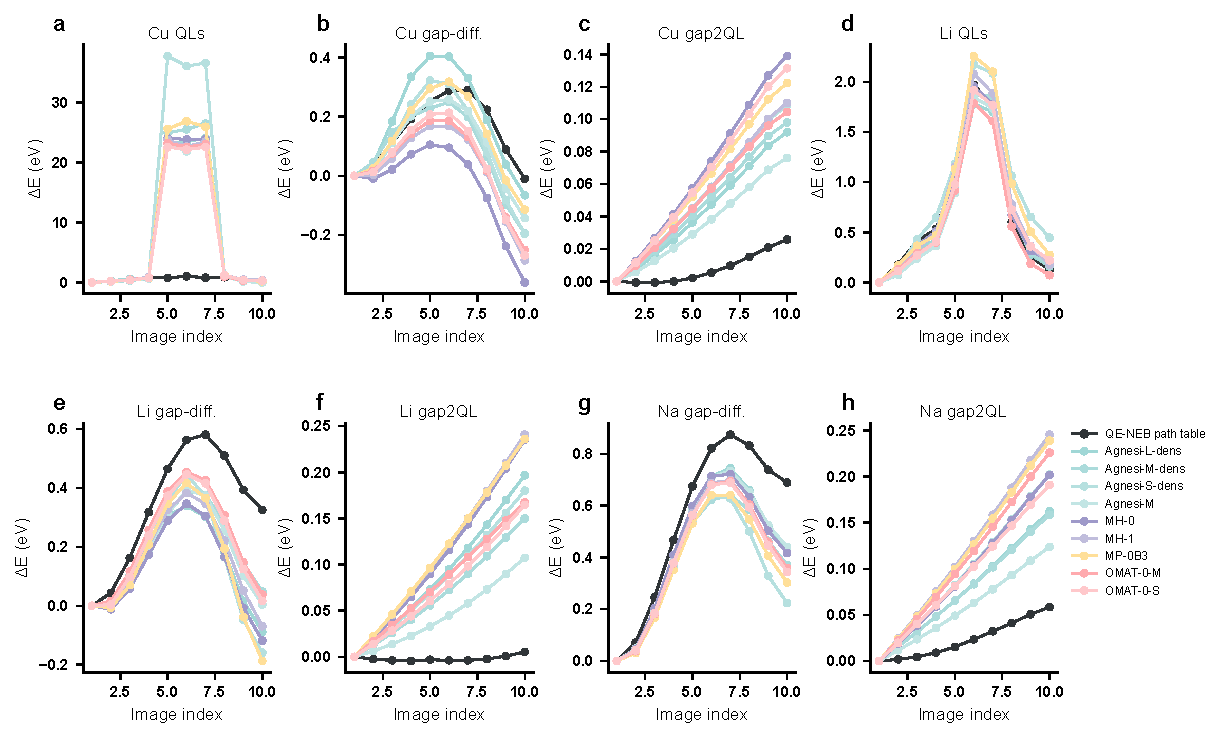
\includegraphics[width=\linewidth,height=0.42\textheight,keepaspectratio]{figure_pages/assets/fig_089.pdf}
\caption{Neb pathway, barrier, topology, or self-consistency diagnostics. This page shows the candidate output ``Figure corrected dft foundation path profiles'' within the audited TASK3-NEB family. The panel identity, source scope, and current status are retained in the accompanying evidence matrix.}
\label{fig:candidate_089}
\end{figure}
\textbf{Results text draft.} The panels distinguish fixed-path scoring, self-consistent MLFF-NEB behavior, endpoint/path topology checks, and DFT convergence status. These operators answer different questions and are kept separate in the text.
\textbf{Discussion and boundary.} A model-reported self-relaxed barrier must not be presented as the fixed-path DFT error, and a provisional or unconverged DFT path must not be promoted to a final reference barrier.
\textbf{Article placement.} Proposed article location: Results or SI: path-family diagnostics.
\textbf{Reviewer linkage:} overall status PARTIAL.
\begin{itemize}[leftmargin=1.4em,noitemsep]
\item \textbf{REV-A1 (PARTIAL):} Reconcile Fig. 3d fixed-geometry DFT-path scoring with SI Fig. S3 self-consistent MLFF-NEB, including pathway identity and the DFT reference. \emph{Completed:} The fixed-path versus self-relaxed operator distinction and the narrower model-reported-barrier wording are integrated. \emph{Still required:} Close the restartable QE path-1--4 convergence gate, preserve the final path/source metadata, and complete the SI Fig. S3 endpoint/checkpoint/optimizer/source audit before calling the quantitative reference final.
\end{itemize}
\textbf{Evidence pointers.}
\begin{itemize}[leftmargin=1.4em,noitemsep]
\item Data/processed: \begingroup\scriptsize\url{ablation/analysis/task3_endpoint_only_neb/exploratory_energy_audit/audit_summary.json}\endgroup
\item Data/processed: \begingroup\scriptsize\url{ablation/analysis/task3_endpoint_only_neb/exploratory_energy_audit/corrected_dft_foundation_models/corrected_dft_foundation_image_profiles.csv}\endgroup
\item Plot/processing script: \begingroup\scriptsize\url{ablation/analysis/task3_endpoint_only_neb/exploratory_energy_audit/plot_paper_figures.py}\endgroup
\item Caption/text source: \begingroup\scriptsize\url{ablation/analysis/task3_endpoint_only_neb/exploratory_energy_audit/ACCEPTANCE_MATRIX.md}\endgroup
\item Caption/text source: \begingroup\scriptsize\url{ablation/analysis/task3_endpoint_only_neb/exploratory_energy_audit/EXPLORATORY_REPORT.md}\endgroup
\end{itemize}
\statusline{\textbf{Audit gap / next action:} Many per-path exports have no co-located generator; use the parent renderer and record the exact input tables}
\vfill
\clearpage
\section{FIG-090 --- Figure diagnostic framework overview}
\label{figpage:fig-090}
\textbf{Group:} TASK3-NEB\quad \textbf{Evidence chain:} partial\quad \textbf{Status:} exploratory;audit
\begin{figure}[H]
\centering
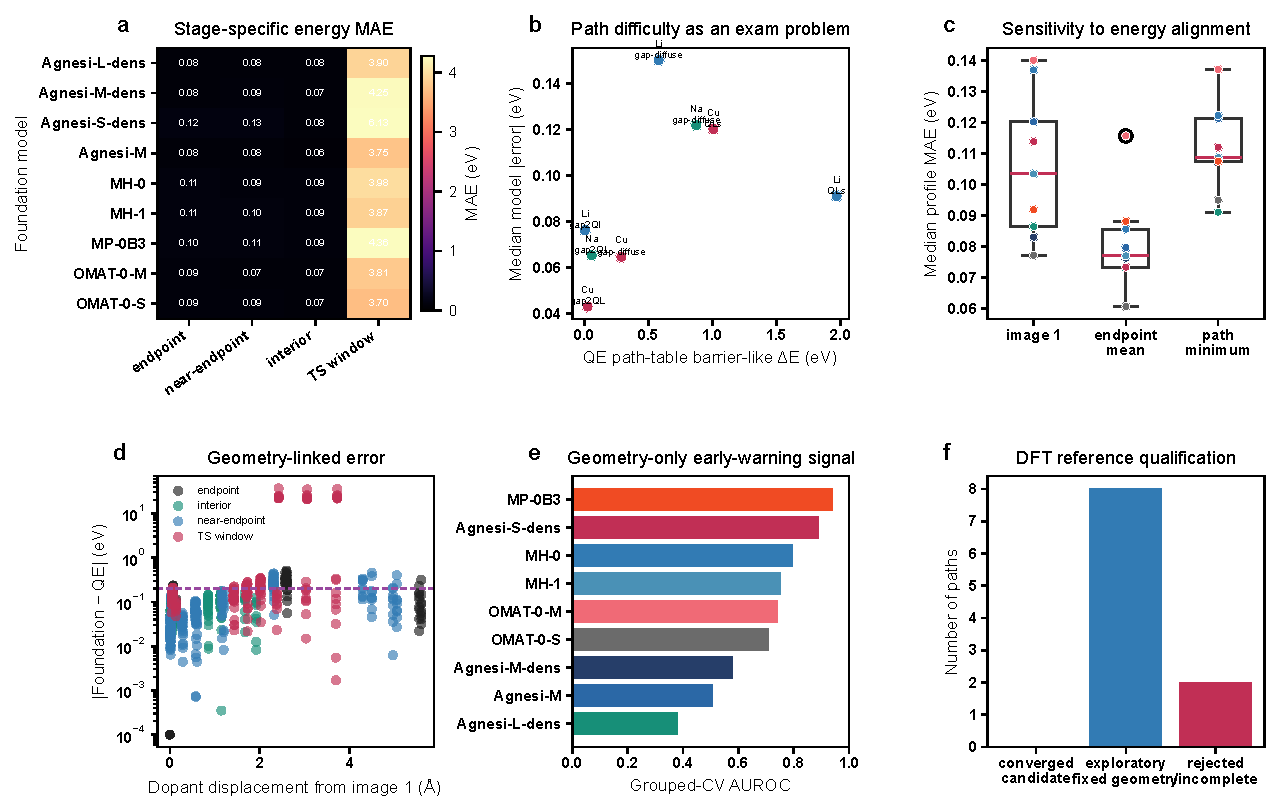
\includegraphics[width=\linewidth,height=0.42\textheight,keepaspectratio]{figure_pages/assets/fig_090.pdf}
\caption{Neb pathway, barrier, topology, or self-consistency diagnostics. This page shows the candidate output ``Figure diagnostic framework overview'' within the audited TASK3-NEB family. The panel identity, source scope, and current status are retained in the accompanying evidence matrix.}
\label{fig:candidate_090}
\end{figure}
\textbf{Results text draft.} The panels distinguish fixed-path scoring, self-consistent MLFF-NEB behavior, endpoint/path topology checks, and DFT convergence status. These operators answer different questions and are kept separate in the text.
\textbf{Discussion and boundary.} A model-reported self-relaxed barrier must not be presented as the fixed-path DFT error, and a provisional or unconverged DFT path must not be promoted to a final reference barrier.
\textbf{Article placement.} Proposed article location: Results or SI: path-family diagnostics.
\textbf{Reviewer linkage:} overall status PARTIAL.
\begin{itemize}[leftmargin=1.4em,noitemsep]
\item \textbf{REV-A1 (PARTIAL):} Reconcile Fig. 3d fixed-geometry DFT-path scoring with SI Fig. S3 self-consistent MLFF-NEB, including pathway identity and the DFT reference. \emph{Completed:} The fixed-path versus self-relaxed operator distinction and the narrower model-reported-barrier wording are integrated. \emph{Still required:} Close the restartable QE path-1--4 convergence gate, preserve the final path/source metadata, and complete the SI Fig. S3 endpoint/checkpoint/optimizer/source audit before calling the quantitative reference final.
\end{itemize}
\textbf{Evidence pointers.}
\begin{itemize}[leftmargin=1.4em,noitemsep]
\item Data/processed: \begingroup\scriptsize\url{ablation/analysis/task3_endpoint_only_neb/exploratory_energy_audit/audit_summary.json}\endgroup
\item Data/processed: \begingroup\scriptsize\url{ablation/analysis/task3_endpoint_only_neb/exploratory_energy_audit/diagnostic_framework/alignment_profile_errors.csv}\endgroup
\item Plot/processing script: \begingroup\scriptsize\url{ablation/analysis/task3_endpoint_only_neb/exploratory_energy_audit/plot_paper_figures.py}\endgroup
\item Caption/text source: \begingroup\scriptsize\url{ablation/analysis/task3_endpoint_only_neb/exploratory_energy_audit/ACCEPTANCE_MATRIX.md}\endgroup
\item Caption/text source: \begingroup\scriptsize\url{ablation/analysis/task3_endpoint_only_neb/exploratory_energy_audit/EXPLORATORY_REPORT.md}\endgroup
\end{itemize}
\statusline{\textbf{Audit gap / next action:} Many per-path exports have no co-located generator; use the parent renderer and record the exact input tables}
\vfill
\clearpage
\section{FIG-091 --- Figure1 task type matrix}
\label{figpage:fig-091}
\textbf{Group:} TASK3-NEB\quad \textbf{Evidence chain:} partial\quad \textbf{Status:} exploratory;audit
\begin{figure}[H]
\centering
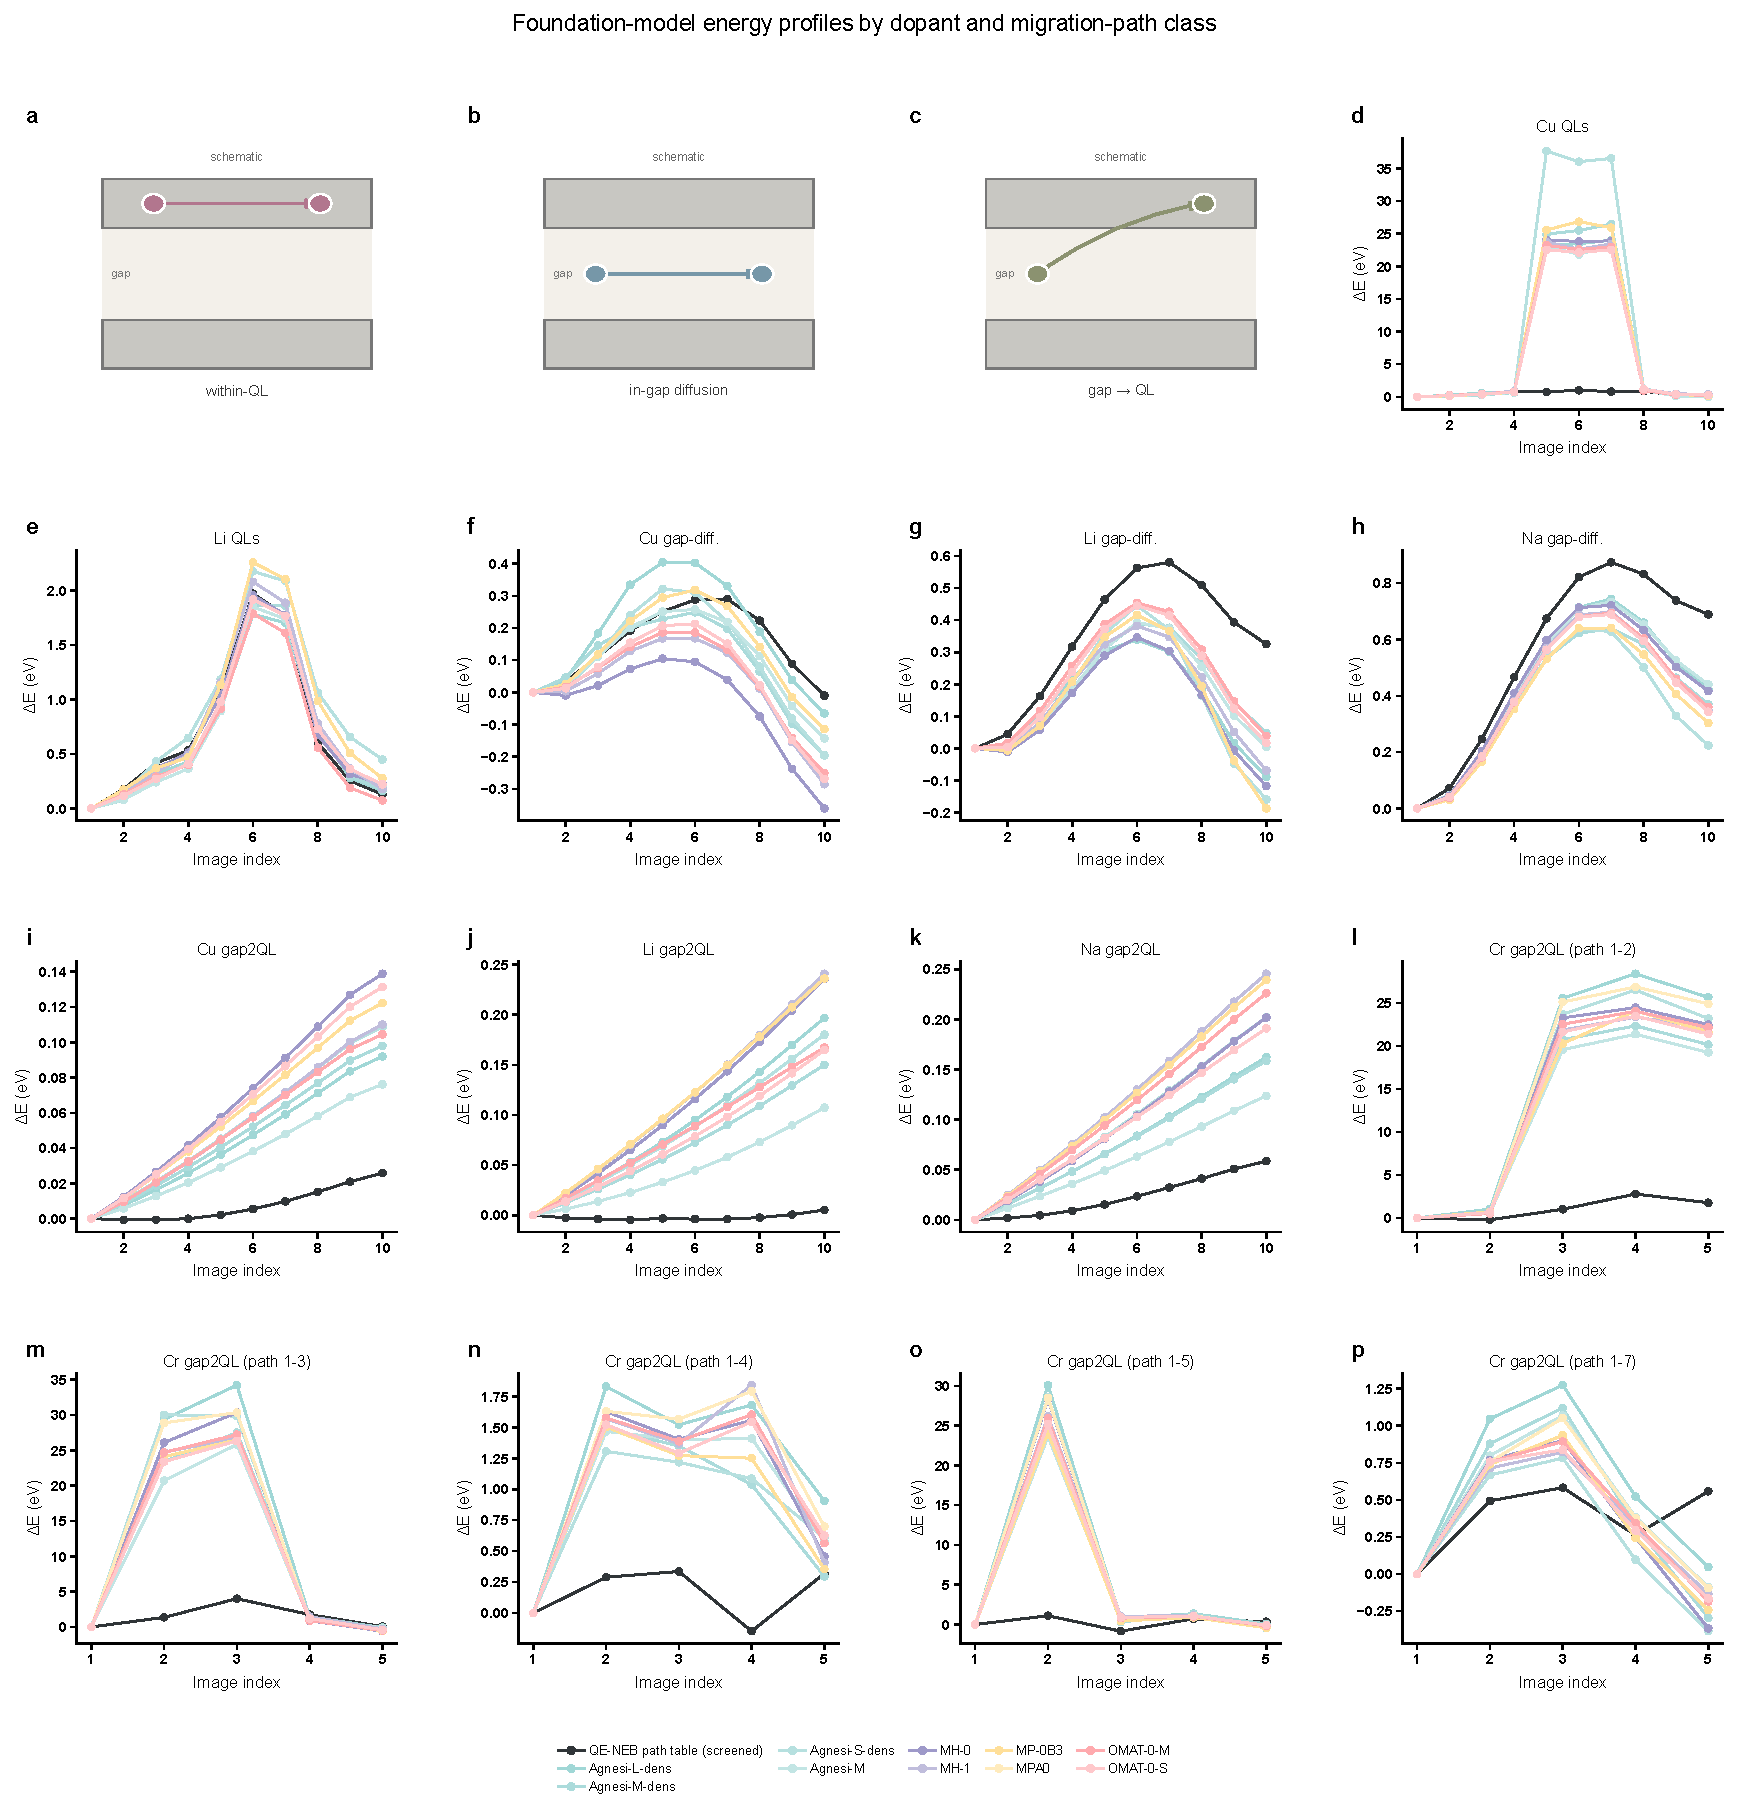
\includegraphics[width=\linewidth,height=0.42\textheight,keepaspectratio]{figure_pages/assets/fig_091.pdf}
\caption{Neb pathway, barrier, topology, or self-consistency diagnostics. This page shows the candidate output ``Figure1 task type matrix'' within the audited TASK3-NEB family. The panel identity, source scope, and current status are retained in the accompanying evidence matrix.}
\label{fig:candidate_091}
\end{figure}
\textbf{Results text draft.} The panels distinguish fixed-path scoring, self-consistent MLFF-NEB behavior, endpoint/path topology checks, and DFT convergence status. These operators answer different questions and are kept separate in the text.
\textbf{Discussion and boundary.} A model-reported self-relaxed barrier must not be presented as the fixed-path DFT error, and a provisional or unconverged DFT path must not be promoted to a final reference barrier.
\textbf{Article placement.} Proposed article location: Results or SI: path-family diagnostics.
\textbf{Reviewer linkage:} overall status PARTIAL.
\begin{itemize}[leftmargin=1.4em,noitemsep]
\item \textbf{REV-A1 (PARTIAL):} Reconcile Fig. 3d fixed-geometry DFT-path scoring with SI Fig. S3 self-consistent MLFF-NEB, including pathway identity and the DFT reference. \emph{Completed:} The fixed-path versus self-relaxed operator distinction and the narrower model-reported-barrier wording are integrated. \emph{Still required:} Close the restartable QE path-1--4 convergence gate, preserve the final path/source metadata, and complete the SI Fig. S3 endpoint/checkpoint/optimizer/source audit before calling the quantitative reference final.
\end{itemize}
\textbf{Evidence pointers.}
\begin{itemize}[leftmargin=1.4em,noitemsep]
\item Data/processed: \begingroup\scriptsize\url{ablation/analysis/task3_endpoint_only_neb/exploratory_energy_audit/audit_summary.json}\endgroup
\item Data/processed: \begingroup\scriptsize\url{ablation/analysis/task3_endpoint_only_neb/exploratory_energy_audit/figure1_task_type_matrix/cr_foundation_path_barriers.csv}\endgroup
\item Plot/processing script: \begingroup\scriptsize\url{ablation/analysis/task3_endpoint_only_neb/exploratory_energy_audit/plot_paper_figures.py}\endgroup
\item Caption/text source: \begingroup\scriptsize\url{ablation/analysis/task3_endpoint_only_neb/exploratory_energy_audit/ACCEPTANCE_MATRIX.md}\endgroup
\item Caption/text source: \begingroup\scriptsize\url{ablation/analysis/task3_endpoint_only_neb/exploratory_energy_audit/EXPLORATORY_REPORT.md}\endgroup
\end{itemize}
\statusline{\textbf{Audit gap / next action:} Many per-path exports have no co-located generator; use the parent renderer and record the exact input tables}
\vfill
\clearpage
\section{FIG-092 --- Figure all foundation model path profiles}
\label{figpage:fig-092}
\textbf{Group:} TASK3-NEB\quad \textbf{Evidence chain:} partial\quad \textbf{Status:} exploratory;audit;comparison
\begin{figure}[H]
\centering
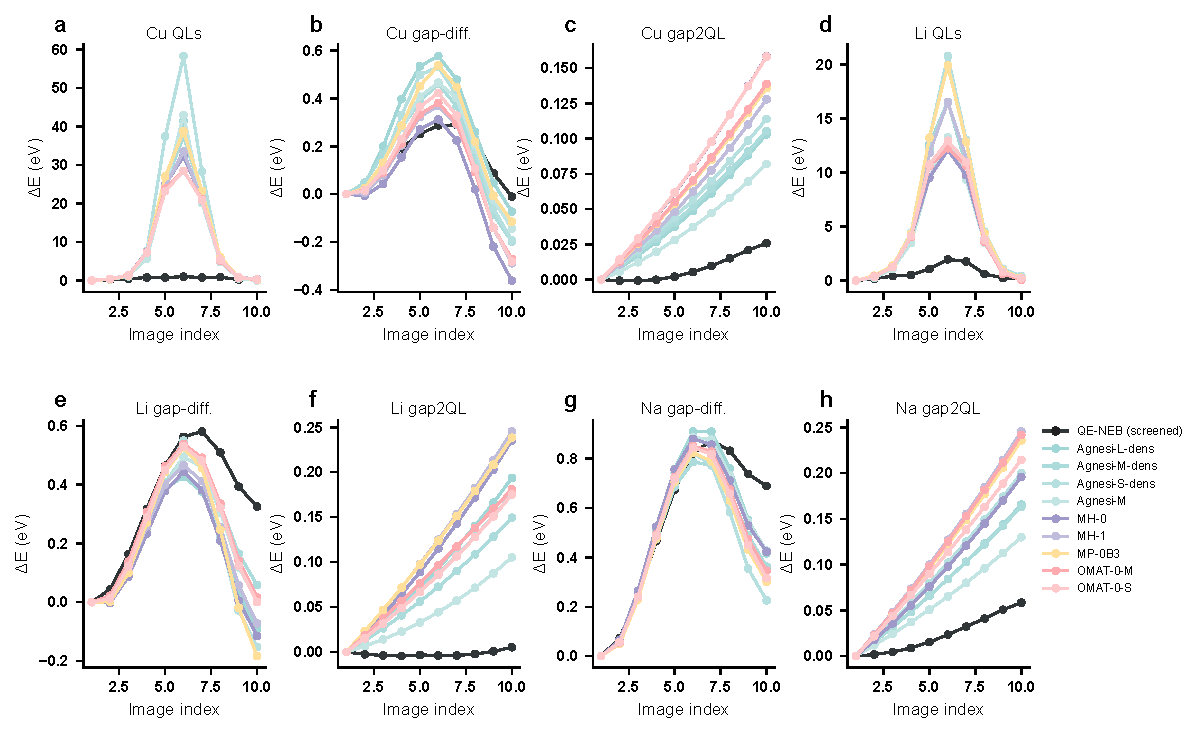
\includegraphics[width=\linewidth,height=0.42\textheight,keepaspectratio]{figure_pages/assets/fig_092.pdf}
\caption{Neb pathway, barrier, topology, or self-consistency diagnostics. This page shows the candidate output ``Figure all foundation model path profiles'' within the audited TASK3-NEB family. The panel identity, source scope, and current status are retained in the accompanying evidence matrix.}
\label{fig:candidate_092}
\end{figure}
\textbf{Results text draft.} The panels distinguish fixed-path scoring, self-consistent MLFF-NEB behavior, endpoint/path topology checks, and DFT convergence status. These operators answer different questions and are kept separate in the text.
\textbf{Discussion and boundary.} A model-reported self-relaxed barrier must not be presented as the fixed-path DFT error, and a provisional or unconverged DFT path must not be promoted to a final reference barrier.
\textbf{Article placement.} Proposed article location: Results or SI: path-family diagnostics.
\textbf{Reviewer linkage:} overall status PARTIAL.
\begin{itemize}[leftmargin=1.4em,noitemsep]
\item \textbf{REV-A1 (PARTIAL):} Reconcile Fig. 3d fixed-geometry DFT-path scoring with SI Fig. S3 self-consistent MLFF-NEB, including pathway identity and the DFT reference. \emph{Completed:} The fixed-path versus self-relaxed operator distinction and the narrower model-reported-barrier wording are integrated. \emph{Still required:} Close the restartable QE path-1--4 convergence gate, preserve the final path/source metadata, and complete the SI Fig. S3 endpoint/checkpoint/optimizer/source audit before calling the quantitative reference final.
\end{itemize}
\textbf{Evidence pointers.}
\begin{itemize}[leftmargin=1.4em,noitemsep]
\item Data/processed: \begingroup\scriptsize\url{ablation/analysis/task3_endpoint_only_neb/exploratory_energy_audit/audit_summary.json}\endgroup
\item Data/processed: \begingroup\scriptsize\url{ablation/analysis/task3_endpoint_only_neb/exploratory_energy_audit/full_foundation_models/all_foundation_model_image_profiles.csv}\endgroup
\item Plot/processing script: \begingroup\scriptsize\url{ablation/analysis/task3_endpoint_only_neb/exploratory_energy_audit/plot_paper_figures.py}\endgroup
\item Caption/text source: \begingroup\scriptsize\url{ablation/analysis/task3_endpoint_only_neb/exploratory_energy_audit/ACCEPTANCE_MATRIX.md}\endgroup
\item Caption/text source: \begingroup\scriptsize\url{ablation/analysis/task3_endpoint_only_neb/exploratory_energy_audit/EXPLORATORY_REPORT.md}\endgroup
\end{itemize}
\statusline{\textbf{Audit gap / next action:} Many per-path exports have no co-located generator; use the parent renderer and record the exact input tables}
\vfill
\clearpage
\section{FIG-093 --- Figure all foundation model spread}
\label{figpage:fig-093}
\textbf{Group:} TASK3-NEB\quad \textbf{Evidence chain:} partial\quad \textbf{Status:} exploratory;audit
\begin{figure}[H]
\centering
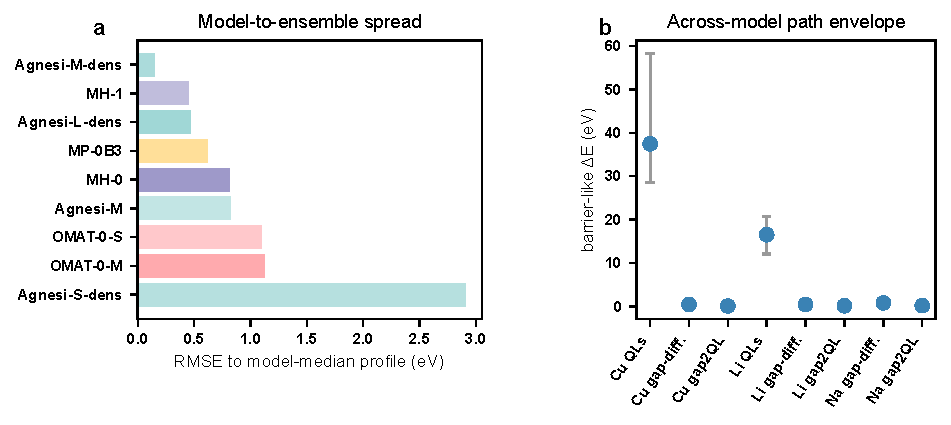
\includegraphics[width=\linewidth,height=0.42\textheight,keepaspectratio]{figure_pages/assets/fig_093.pdf}
\caption{Neb pathway, barrier, topology, or self-consistency diagnostics. This page shows the candidate output ``Figure all foundation model spread'' within the audited TASK3-NEB family. The panel identity, source scope, and current status are retained in the accompanying evidence matrix.}
\label{fig:candidate_093}
\end{figure}
\textbf{Results text draft.} The panels distinguish fixed-path scoring, self-consistent MLFF-NEB behavior, endpoint/path topology checks, and DFT convergence status. These operators answer different questions and are kept separate in the text.
\textbf{Discussion and boundary.} A model-reported self-relaxed barrier must not be presented as the fixed-path DFT error, and a provisional or unconverged DFT path must not be promoted to a final reference barrier.
\textbf{Article placement.} Proposed article location: Results or SI: path-family diagnostics.
\textbf{Reviewer linkage:} overall status PARTIAL.
\begin{itemize}[leftmargin=1.4em,noitemsep]
\item \textbf{REV-A1 (PARTIAL):} Reconcile Fig. 3d fixed-geometry DFT-path scoring with SI Fig. S3 self-consistent MLFF-NEB, including pathway identity and the DFT reference. \emph{Completed:} The fixed-path versus self-relaxed operator distinction and the narrower model-reported-barrier wording are integrated. \emph{Still required:} Close the restartable QE path-1--4 convergence gate, preserve the final path/source metadata, and complete the SI Fig. S3 endpoint/checkpoint/optimizer/source audit before calling the quantitative reference final.
\end{itemize}
\textbf{Evidence pointers.}
\begin{itemize}[leftmargin=1.4em,noitemsep]
\item Data/processed: \begingroup\scriptsize\url{ablation/analysis/task3_endpoint_only_neb/exploratory_energy_audit/audit_summary.json}\endgroup
\item Data/processed: \begingroup\scriptsize\url{ablation/analysis/task3_endpoint_only_neb/exploratory_energy_audit/full_foundation_models/all_foundation_model_image_profiles.csv}\endgroup
\item Plot/processing script: \begingroup\scriptsize\url{ablation/analysis/task3_endpoint_only_neb/exploratory_energy_audit/plot_paper_figures.py}\endgroup
\item Caption/text source: \begingroup\scriptsize\url{ablation/analysis/task3_endpoint_only_neb/exploratory_energy_audit/ACCEPTANCE_MATRIX.md}\endgroup
\item Caption/text source: \begingroup\scriptsize\url{ablation/analysis/task3_endpoint_only_neb/exploratory_energy_audit/EXPLORATORY_REPORT.md}\endgroup
\end{itemize}
\statusline{\textbf{Audit gap / next action:} Many per-path exports have no co-located generator; use the parent renderer and record the exact input tables}
\vfill
\clearpage
\section{FIG-094 --- Figure neb residual audit}
\label{figpage:fig-094}
\textbf{Group:} TASK3-NEB\quad \textbf{Evidence chain:} partial\quad \textbf{Status:} exploratory;audit
\begin{figure}[H]
\centering
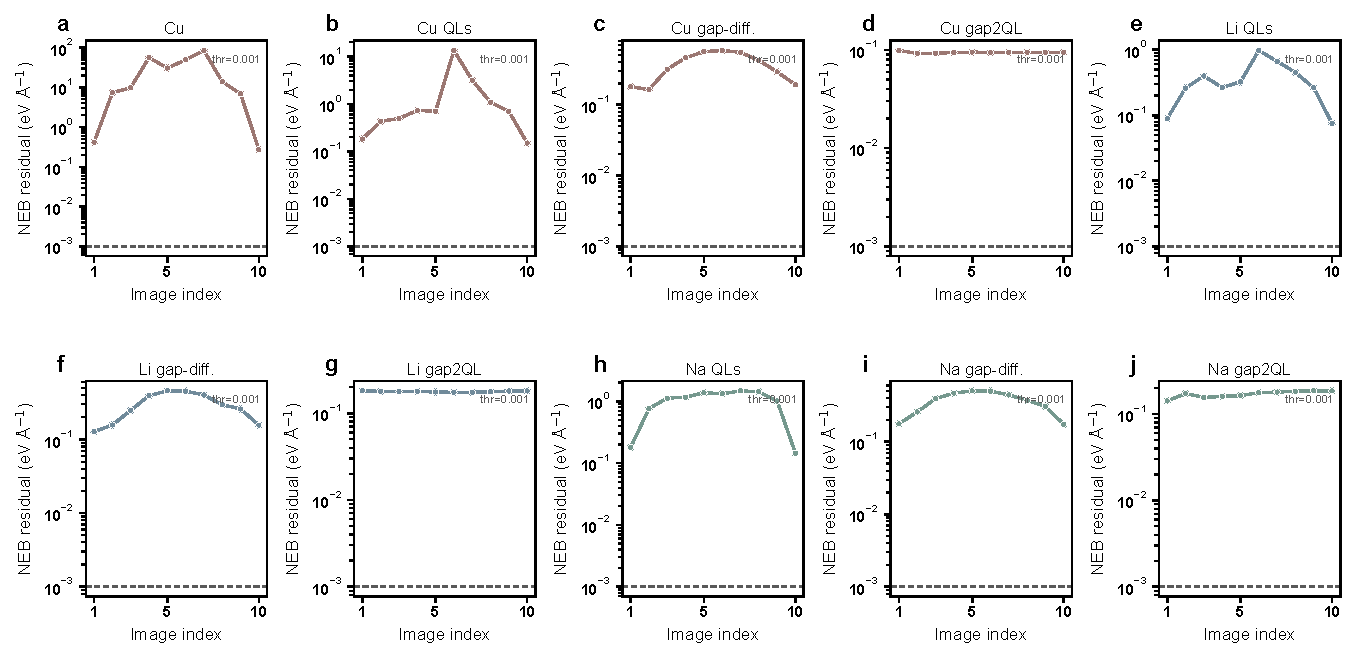
\includegraphics[width=\linewidth,height=0.42\textheight,keepaspectratio]{figure_pages/assets/fig_094.pdf}
\caption{Neb pathway, barrier, topology, or self-consistency diagnostics. This page shows the candidate output ``Figure neb residual audit'' within the audited TASK3-NEB family. The panel identity, source scope, and current status are retained in the accompanying evidence matrix.}
\label{fig:candidate_094}
\end{figure}
\textbf{Results text draft.} The panels distinguish fixed-path scoring, self-consistent MLFF-NEB behavior, endpoint/path topology checks, and DFT convergence status. These operators answer different questions and are kept separate in the text.
\textbf{Discussion and boundary.} A model-reported self-relaxed barrier must not be presented as the fixed-path DFT error, and a provisional or unconverged DFT path must not be promoted to a final reference barrier.
\textbf{Article placement.} Proposed article location: Results or SI: path-family diagnostics.
\textbf{Reviewer linkage:} overall status PARTIAL.
\begin{itemize}[leftmargin=1.4em,noitemsep]
\item \textbf{REV-A1 (PARTIAL):} Reconcile Fig. 3d fixed-geometry DFT-path scoring with SI Fig. S3 self-consistent MLFF-NEB, including pathway identity and the DFT reference. \emph{Completed:} The fixed-path versus self-relaxed operator distinction and the narrower model-reported-barrier wording are integrated. \emph{Still required:} Close the restartable QE path-1--4 convergence gate, preserve the final path/source metadata, and complete the SI Fig. S3 endpoint/checkpoint/optimizer/source audit before calling the quantitative reference final.
\end{itemize}
\textbf{Evidence pointers.}
\begin{itemize}[leftmargin=1.4em,noitemsep]
\item Data/processed: \begingroup\scriptsize\url{ablation/analysis/task3_endpoint_only_neb/exploratory_energy_audit/audit_summary.json}\endgroup
\item Data/processed: \begingroup\scriptsize\url{ablation/analysis/task3_endpoint_only_neb/exploratory_energy_audit/neb_convergence_audit/qe_neb_image_residual_audit.csv}\endgroup
\item Plot/processing script: \begingroup\scriptsize\url{ablation/analysis/task3_endpoint_only_neb/exploratory_energy_audit/plot_paper_figures.py}\endgroup
\item Caption/text source: \begingroup\scriptsize\url{ablation/analysis/task3_endpoint_only_neb/exploratory_energy_audit/ACCEPTANCE_MATRIX.md}\endgroup
\item Caption/text source: \begingroup\scriptsize\url{ablation/analysis/task3_endpoint_only_neb/exploratory_energy_audit/EXPLORATORY_REPORT.md}\endgroup
\end{itemize}
\statusline{\textbf{Audit gap / next action:} Many per-path exports have no co-located generator; use the parent renderer and record the exact input tables}
\vfill
\clearpage
\section{FIG-095 --- Figure 1 stability parity perturbation}
\label{figpage:fig-095}
\textbf{Group:} TASK3-NEB\quad \textbf{Evidence chain:} partial\quad \textbf{Status:} exploratory;audit;comparison
\begin{figure}[H]
\centering
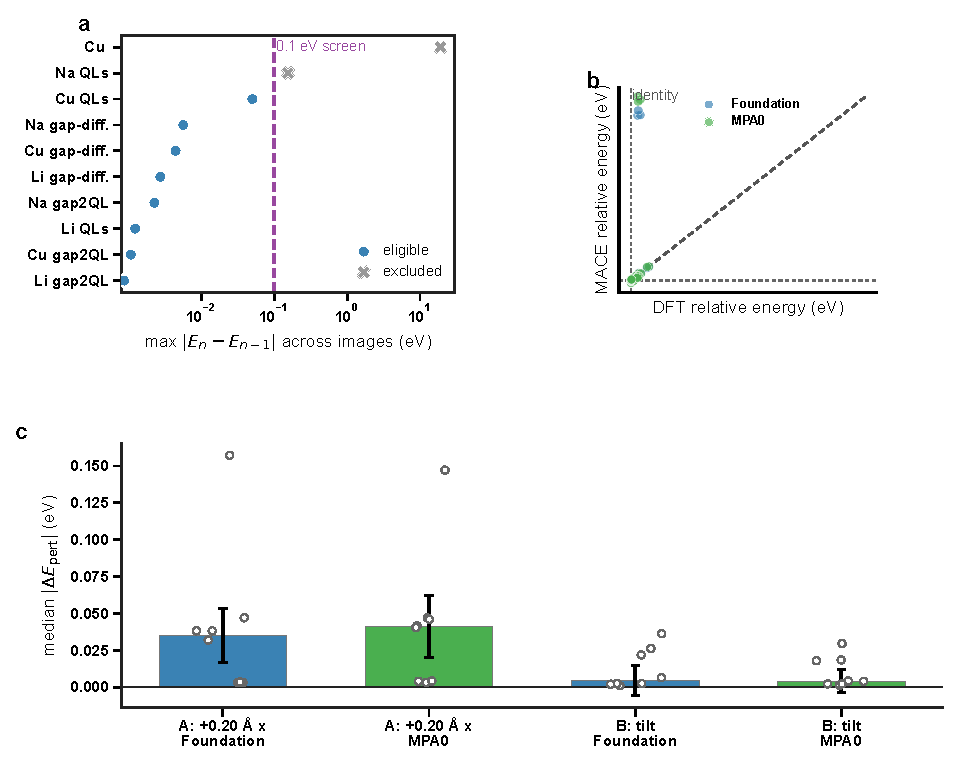
\includegraphics[width=\linewidth,height=0.42\textheight,keepaspectratio]{figure_pages/assets/fig_095.pdf}
\caption{Neb pathway, barrier, topology, or self-consistency diagnostics. This page shows the candidate output ``Figure 1 stability parity perturbation'' within the audited TASK3-NEB family. The panel identity, source scope, and current status are retained in the accompanying evidence matrix.}
\label{fig:candidate_095}
\end{figure}
\textbf{Results text draft.} The panels distinguish fixed-path scoring, self-consistent MLFF-NEB behavior, endpoint/path topology checks, and DFT convergence status. These operators answer different questions and are kept separate in the text.
\textbf{Discussion and boundary.} A model-reported self-relaxed barrier must not be presented as the fixed-path DFT error, and a provisional or unconverged DFT path must not be promoted to a final reference barrier.
\textbf{Article placement.} Proposed article location: Results or SI: path-family diagnostics.
\textbf{Reviewer linkage:} overall status PARTIAL.
\begin{itemize}[leftmargin=1.4em,noitemsep]
\item \textbf{REV-A1 (PARTIAL):} Reconcile Fig. 3d fixed-geometry DFT-path scoring with SI Fig. S3 self-consistent MLFF-NEB, including pathway identity and the DFT reference. \emph{Completed:} The fixed-path versus self-relaxed operator distinction and the narrower model-reported-barrier wording are integrated. \emph{Still required:} Close the restartable QE path-1--4 convergence gate, preserve the final path/source metadata, and complete the SI Fig. S3 endpoint/checkpoint/optimizer/source audit before calling the quantitative reference final.
\end{itemize}
\textbf{Evidence pointers.}
\begin{itemize}[leftmargin=1.4em,noitemsep]
\item Data/processed: \begingroup\scriptsize\url{ablation/analysis/task3_endpoint_only_neb/exploratory_energy_audit/processed/analysis_manifest.json}\endgroup
\item Data/processed: \begingroup\scriptsize\url{ablation/analysis/task3_endpoint_only_neb/exploratory_energy_audit/processed/figures/table_1_model_summary.csv}\endgroup
\item Caption/text source: \begingroup\scriptsize\url{ablation/analysis/task3_endpoint_only_neb/exploratory_energy_audit/processed/figures/captions_and_discussion.md}\endgroup
\item Caption/text source: \begingroup\scriptsize\url{ablation/analysis/task3_endpoint_only_neb/exploratory_energy_audit/processed/figures/table_1_model_summary.tex}\endgroup
\end{itemize}
\statusline{\textbf{Audit gap / next action:} Many per-path exports have no co-located generator; use the parent renderer and record the exact input tables}
\vfill
\clearpage
\section{FIG-096 --- Figure 2 relative energy profiles}
\label{figpage:fig-096}
\textbf{Group:} TASK3-NEB\quad \textbf{Evidence chain:} partial\quad \textbf{Status:} exploratory;audit;comparison
\begin{figure}[H]
\centering
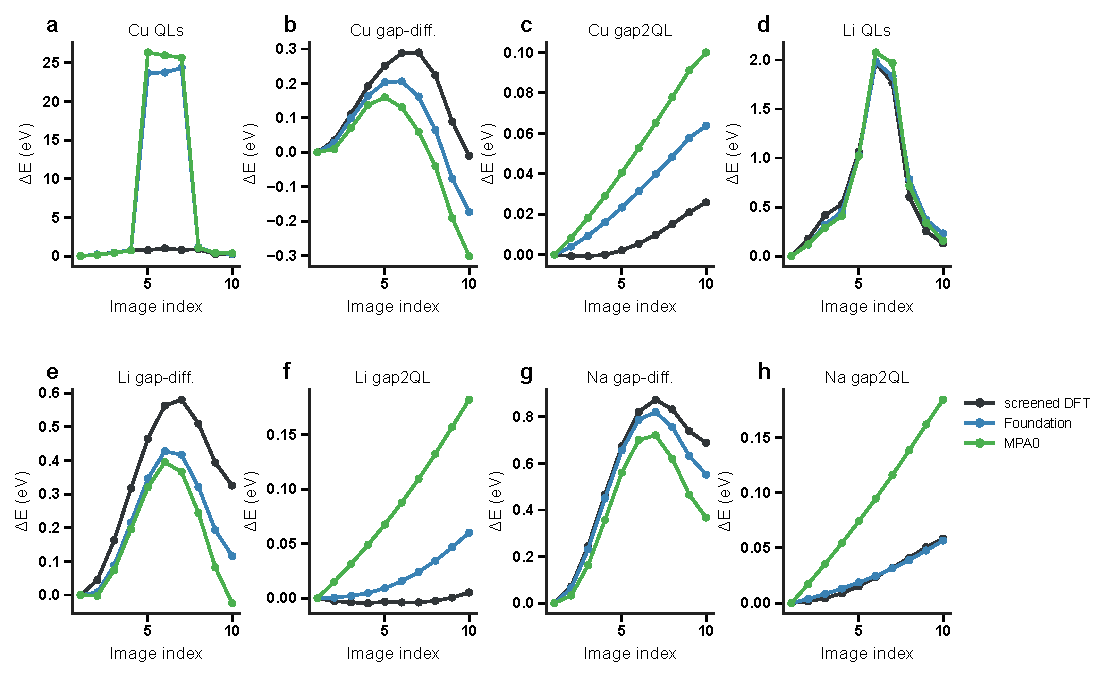
\includegraphics[width=\linewidth,height=0.42\textheight,keepaspectratio]{figure_pages/assets/fig_096.pdf}
\caption{Neb pathway, barrier, topology, or self-consistency diagnostics. This page shows the candidate output ``Figure 2 relative energy profiles'' within the audited TASK3-NEB family. The panel identity, source scope, and current status are retained in the accompanying evidence matrix.}
\label{fig:candidate_096}
\end{figure}
\textbf{Results text draft.} The panels distinguish fixed-path scoring, self-consistent MLFF-NEB behavior, endpoint/path topology checks, and DFT convergence status. These operators answer different questions and are kept separate in the text.
\textbf{Discussion and boundary.} A model-reported self-relaxed barrier must not be presented as the fixed-path DFT error, and a provisional or unconverged DFT path must not be promoted to a final reference barrier.
\textbf{Article placement.} Proposed article location: Results or SI: path-family diagnostics.
\textbf{Reviewer linkage:} overall status PARTIAL.
\begin{itemize}[leftmargin=1.4em,noitemsep]
\item \textbf{REV-A1 (PARTIAL):} Reconcile Fig. 3d fixed-geometry DFT-path scoring with SI Fig. S3 self-consistent MLFF-NEB, including pathway identity and the DFT reference. \emph{Completed:} The fixed-path versus self-relaxed operator distinction and the narrower model-reported-barrier wording are integrated. \emph{Still required:} Close the restartable QE path-1--4 convergence gate, preserve the final path/source metadata, and complete the SI Fig. S3 endpoint/checkpoint/optimizer/source audit before calling the quantitative reference final.
\end{itemize}
\textbf{Evidence pointers.}
\begin{itemize}[leftmargin=1.4em,noitemsep]
\item Data/processed: \begingroup\scriptsize\url{ablation/analysis/task3_endpoint_only_neb/exploratory_energy_audit/processed/analysis_manifest.json}\endgroup
\item Data/processed: \begingroup\scriptsize\url{ablation/analysis/task3_endpoint_only_neb/exploratory_energy_audit/processed/figures/table_1_model_summary.csv}\endgroup
\item Caption/text source: \begingroup\scriptsize\url{ablation/analysis/task3_endpoint_only_neb/exploratory_energy_audit/processed/figures/captions_and_discussion.md}\endgroup
\item Caption/text source: \begingroup\scriptsize\url{ablation/analysis/task3_endpoint_only_neb/exploratory_energy_audit/processed/figures/table_1_model_summary.tex}\endgroup
\end{itemize}
\statusline{\textbf{Audit gap / next action:} Many per-path exports have no co-located generator; use the parent renderer and record the exact input tables}
\vfill
\clearpage
\section{FIG-097 --- Figure structural stage diagnostics}
\label{figpage:fig-097}
\textbf{Group:} TASK3-NEB\quad \textbf{Evidence chain:} partial\quad \textbf{Status:} exploratory;audit
\begin{figure}[H]
\centering
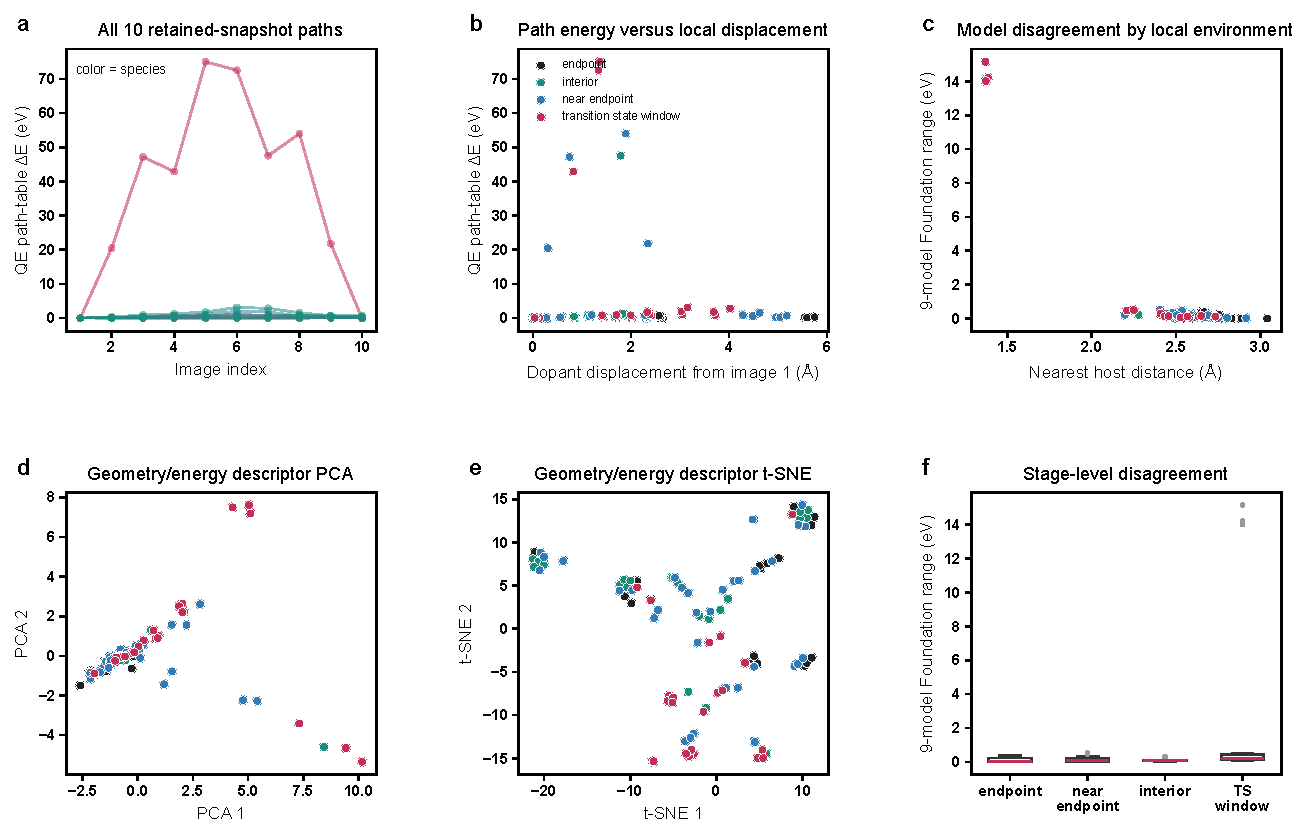
\includegraphics[width=\linewidth,height=0.42\textheight,keepaspectratio]{figure_pages/assets/fig_097.pdf}
\caption{Neb pathway, barrier, topology, or self-consistency diagnostics. This page shows the candidate output ``Figure structural stage diagnostics'' within the audited TASK3-NEB family. The panel identity, source scope, and current status are retained in the accompanying evidence matrix.}
\label{fig:candidate_097}
\end{figure}
\textbf{Results text draft.} The panels distinguish fixed-path scoring, self-consistent MLFF-NEB behavior, endpoint/path topology checks, and DFT convergence status. These operators answer different questions and are kept separate in the text.
\textbf{Discussion and boundary.} A model-reported self-relaxed barrier must not be presented as the fixed-path DFT error, and a provisional or unconverged DFT path must not be promoted to a final reference barrier.
\textbf{Article placement.} Proposed article location: Results or SI: path-family diagnostics.
\textbf{Reviewer linkage:} overall status PARTIAL.
\begin{itemize}[leftmargin=1.4em,noitemsep]
\item \textbf{REV-A1 (PARTIAL):} Reconcile Fig. 3d fixed-geometry DFT-path scoring with SI Fig. S3 self-consistent MLFF-NEB, including pathway identity and the DFT reference. \emph{Completed:} The fixed-path versus self-relaxed operator distinction and the narrower model-reported-barrier wording are integrated. \emph{Still required:} Close the restartable QE path-1--4 convergence gate, preserve the final path/source metadata, and complete the SI Fig. S3 endpoint/checkpoint/optimizer/source audit before calling the quantitative reference final.
\end{itemize}
\textbf{Evidence pointers.}
\begin{itemize}[leftmargin=1.4em,noitemsep]
\item Data/processed: \begingroup\scriptsize\url{ablation/analysis/task3_endpoint_only_neb/exploratory_energy_audit/audit_summary.json}\endgroup
\item Data/processed: \begingroup\scriptsize\url{ablation/analysis/task3_endpoint_only_neb/exploratory_energy_audit/scf_neb_image_energy_deltas.csv}\endgroup
\item Plot/processing script: \begingroup\scriptsize\url{ablation/analysis/task3_endpoint_only_neb/exploratory_energy_audit/plot_paper_figures.py}\endgroup
\item Caption/text source: \begingroup\scriptsize\url{ablation/analysis/task3_endpoint_only_neb/exploratory_energy_audit/ACCEPTANCE_MATRIX.md}\endgroup
\item Caption/text source: \begingroup\scriptsize\url{ablation/analysis/task3_endpoint_only_neb/exploratory_energy_audit/EXPLORATORY_REPORT.md}\endgroup
\end{itemize}
\statusline{\textbf{Audit gap / next action:} Many per-path exports have no co-located generator; use the parent renderer and record the exact input tables}
\vfill
\clearpage
\section{FIG-098 --- Fig1 force disagreement}
\label{figpage:fig-098}
\textbf{Group:} P1-FORCE\quad \textbf{Evidence chain:} traceable\quad \textbf{Status:} publication;comparison
\begin{figure}[H]
\centering
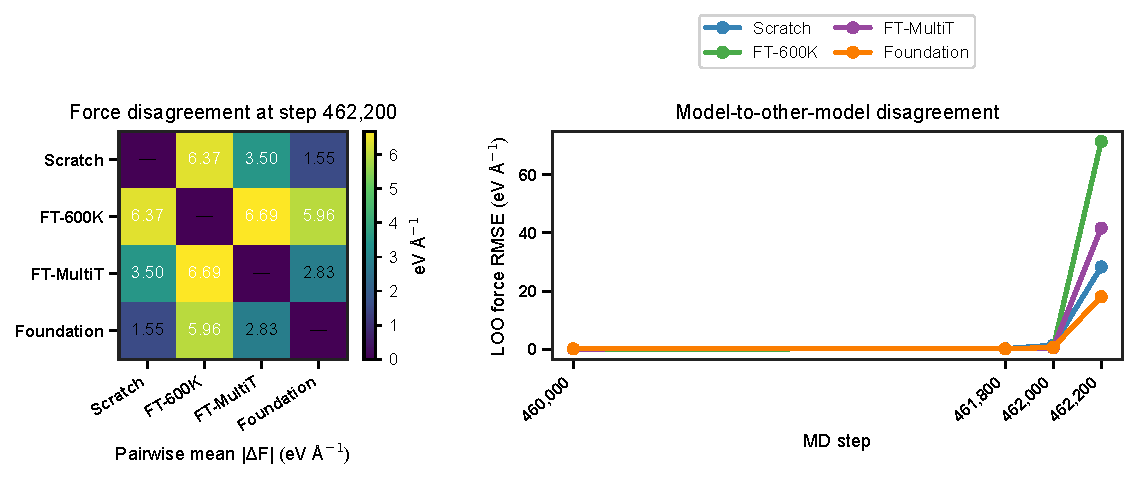
\includegraphics[width=\linewidth,height=0.42\textheight,keepaspectratio]{figure_pages/assets/fig_098.pdf}
\caption{Static force-disagreement and model-transfer diagnostics. This page shows the candidate output ``Fig1 force disagreement'' within the audited P1-FORCE family. The panel identity, source scope, and current status are retained in the accompanying evidence matrix.}
\label{fig:candidate_098}
\end{figure}
\textbf{Results text draft.} The figure compares model forces on a common set of configurations and exposes disagreement patterns that are not reducible to a single aggregate RMSE. The exact sampling scope and model provenance are retained in the evidence row.
\textbf{Discussion and boundary.} This supports the static-reference part of the benchmark. It does not by itself establish stability on a dynamically evolving path or agreement with converged DFT barriers.
\textbf{Article placement.} Proposed article location: Results: model disagreement and trajectory-integrity gate.
\textbf{Reviewer linkage:} overall status NO\_DIRECT\_REVIEWER\_FIGURE\_LINK.
No direct reviewer-response figure linkage was identified; this page is retained for scientific/article audit rather than as a direct reviewer response.
\textbf{Evidence pointers.}
\begin{itemize}[leftmargin=1.4em,noitemsep]
\item Data/processed: \begingroup\scriptsize\url{paper/analysis/phase1_static_force_comparison_20261002/models_local_diagnostic.json}\endgroup
\item Data/processed: \begingroup\scriptsize\url{paper/analysis/phase1_static_force_comparison_20261002/models_rockfish.json}\endgroup
\item Caption/text source: \begingroup\scriptsize\url{paper/analysis/phase1_static_force_comparison_20261002/Methods.md}\endgroup
\item Caption/text source: \begingroup\scriptsize\url{paper/analysis/phase1_static_force_comparison_20261002/README.md}\endgroup
\end{itemize}
\statusline{\textbf{Audit gap / next action:} Duplicate checkout; use current package as canonical}
\vfill
\clearpage
\section{FIG-099 --- Fig2 key local force}
\label{figpage:fig-099}
\textbf{Group:} P1-FORCE\quad \textbf{Evidence chain:} traceable\quad \textbf{Status:} publication;comparison
\begin{figure}[H]
\centering
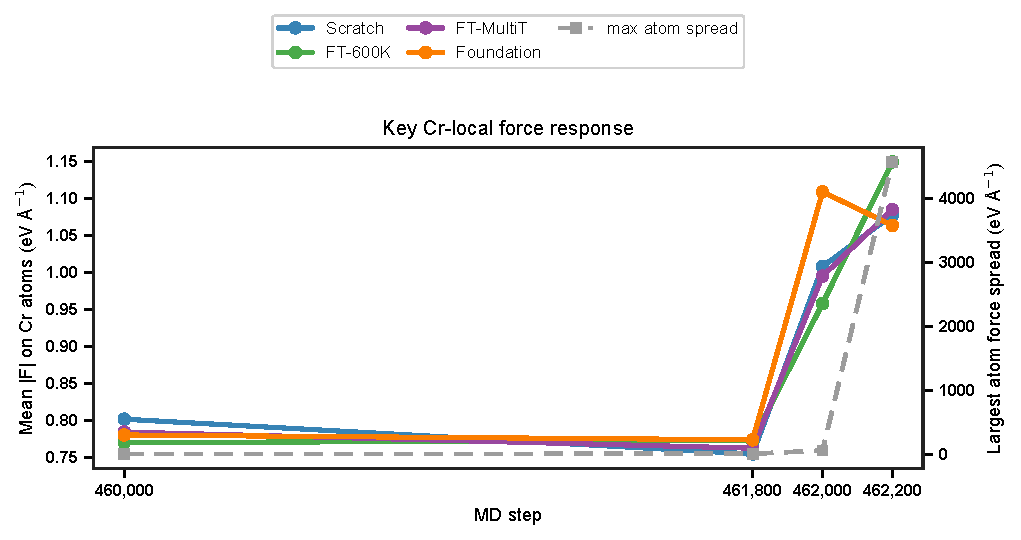
\includegraphics[width=\linewidth,height=0.42\textheight,keepaspectratio]{figure_pages/assets/fig_099.pdf}
\caption{Static force-disagreement and model-transfer diagnostics. This page shows the candidate output ``Fig2 key local force'' within the audited P1-FORCE family. The panel identity, source scope, and current status are retained in the accompanying evidence matrix.}
\label{fig:candidate_099}
\end{figure}
\textbf{Results text draft.} The figure compares model forces on a common set of configurations and exposes disagreement patterns that are not reducible to a single aggregate RMSE. The exact sampling scope and model provenance are retained in the evidence row.
\textbf{Discussion and boundary.} This supports the static-reference part of the benchmark. It does not by itself establish stability on a dynamically evolving path or agreement with converged DFT barriers.
\textbf{Article placement.} Proposed article location: Results: model disagreement and trajectory-integrity gate.
\textbf{Reviewer linkage:} overall status NO\_DIRECT\_REVIEWER\_FIGURE\_LINK.
No direct reviewer-response figure linkage was identified; this page is retained for scientific/article audit rather than as a direct reviewer response.
\textbf{Evidence pointers.}
\begin{itemize}[leftmargin=1.4em,noitemsep]
\item Data/processed: \begingroup\scriptsize\url{paper/analysis/phase1_static_force_comparison_20261002/models_local_diagnostic.json}\endgroup
\item Data/processed: \begingroup\scriptsize\url{paper/analysis/phase1_static_force_comparison_20261002/models_rockfish.json}\endgroup
\item Caption/text source: \begingroup\scriptsize\url{paper/analysis/phase1_static_force_comparison_20261002/Methods.md}\endgroup
\item Caption/text source: \begingroup\scriptsize\url{paper/analysis/phase1_static_force_comparison_20261002/README.md}\endgroup
\end{itemize}
\statusline{\textbf{Audit gap / next action:} Duplicate checkout; use current package as canonical}
\vfill
\clearpage
\section{FIG-100 --- Fig3 geometry step diagnostics}
\label{figpage:fig-100}
\textbf{Group:} P1-FORCE\quad \textbf{Evidence chain:} traceable\quad \textbf{Status:} exploratory;publication;comparison
\begin{figure}[H]
\centering
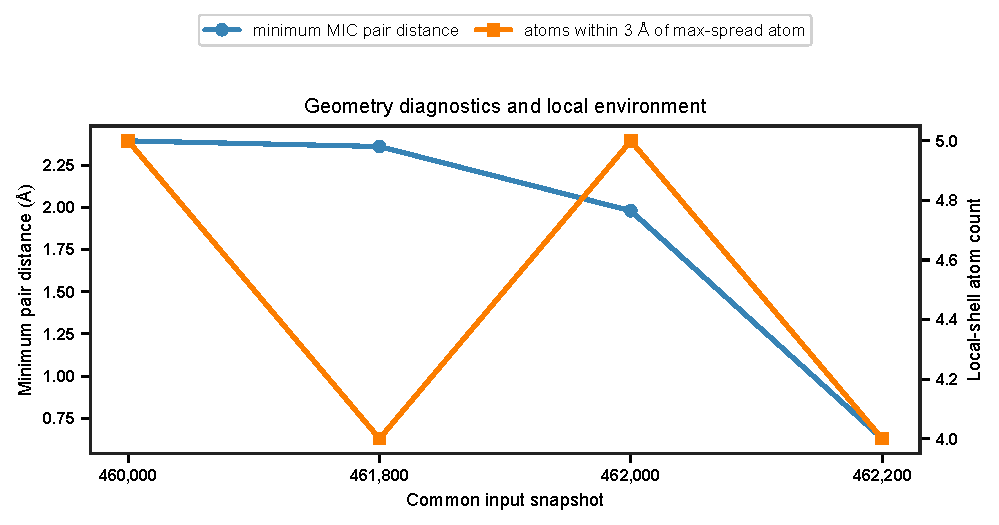
\includegraphics[width=\linewidth,height=0.42\textheight,keepaspectratio]{figure_pages/assets/fig_100.pdf}
\caption{Static force-disagreement and model-transfer diagnostics. This page shows the candidate output ``Fig3 geometry step diagnostics'' within the audited P1-FORCE family. The panel identity, source scope, and current status are retained in the accompanying evidence matrix.}
\label{fig:candidate_100}
\end{figure}
\textbf{Results text draft.} The figure compares model forces on a common set of configurations and exposes disagreement patterns that are not reducible to a single aggregate RMSE. The exact sampling scope and model provenance are retained in the evidence row.
\textbf{Discussion and boundary.} This supports the static-reference part of the benchmark. It does not by itself establish stability on a dynamically evolving path or agreement with converged DFT barriers.
\textbf{Article placement.} Proposed article location: Results: model disagreement and trajectory-integrity gate.
\textbf{Reviewer linkage:} overall status NO\_DIRECT\_REVIEWER\_FIGURE\_LINK.
No direct reviewer-response figure linkage was identified; this page is retained for scientific/article audit rather than as a direct reviewer response.
\textbf{Evidence pointers.}
\begin{itemize}[leftmargin=1.4em,noitemsep]
\item Data/processed: \begingroup\scriptsize\url{paper/analysis/phase1_static_force_comparison_20261002/models_local_diagnostic.json}\endgroup
\item Data/processed: \begingroup\scriptsize\url{paper/analysis/phase1_static_force_comparison_20261002/models_rockfish.json}\endgroup
\item Caption/text source: \begingroup\scriptsize\url{paper/analysis/phase1_static_force_comparison_20261002/Methods.md}\endgroup
\item Caption/text source: \begingroup\scriptsize\url{paper/analysis/phase1_static_force_comparison_20261002/README.md}\endgroup
\end{itemize}
\statusline{\textbf{Audit gap / next action:} Duplicate checkout; use current package as canonical}
\vfill
\clearpage
\section{FIG-101 --- Phase2 handoff timeseries}
\label{figpage:fig-101}
\textbf{Group:} P2-HANDOFF\quad \textbf{Evidence chain:} traceable\quad \textbf{Status:} publication;audit
\begin{figure}[H]
\centering
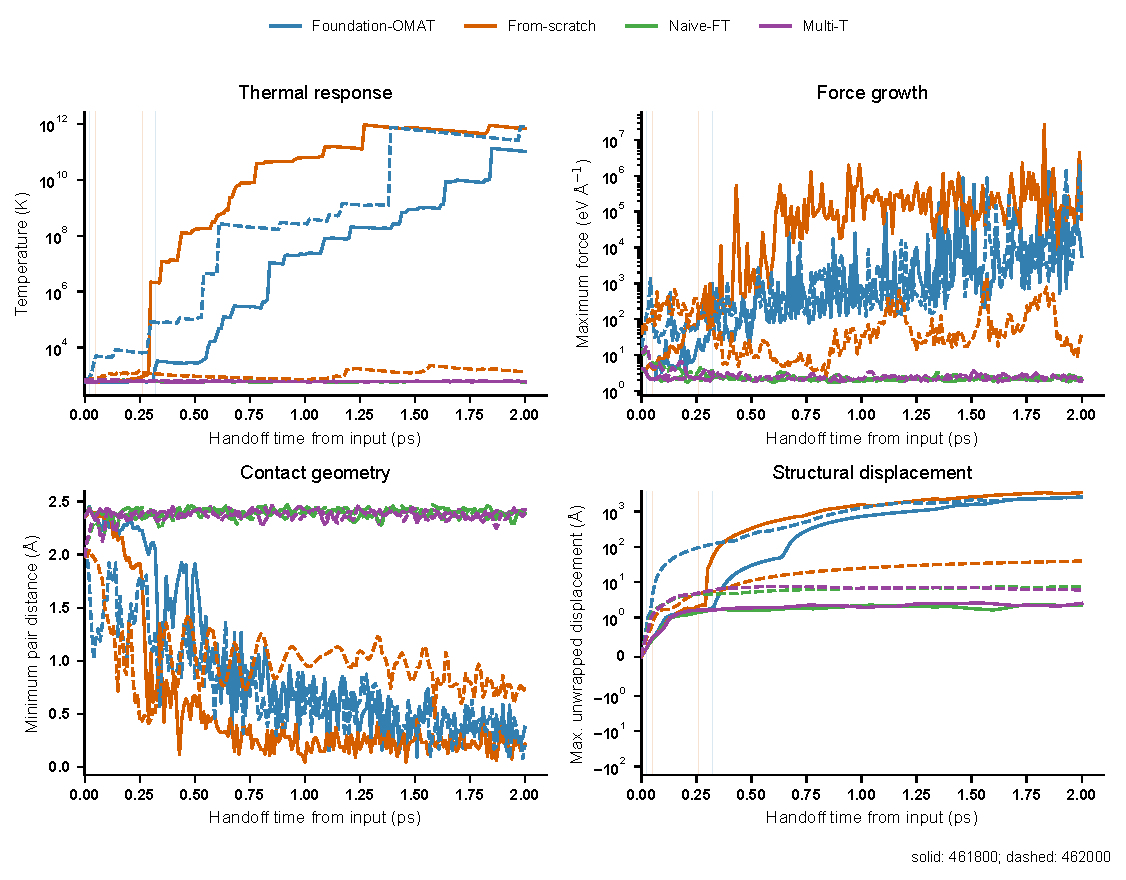
\includegraphics[width=\linewidth,height=0.42\textheight,keepaspectratio]{figure_pages/assets/fig_101.pdf}
\caption{Handoff molecular-dynamics diagnostics and first-divergence audit. This page shows the candidate output ``Phase2 handoff timeseries'' within the audited P2-HANDOFF family. The panel identity, source scope, and current status are retained in the accompanying evidence matrix.}
\label{fig:candidate_101}
\end{figure}
\textbf{Results text draft.} The panels track the temperature, force, contact, and structural observables used to locate the first anomalous behavior after protocol handoff. Run-level integrity and local-neighborhood evidence are kept alongside the visualization.
\textbf{Discussion and boundary.} This is a diagnostic figure for identifying when and how trajectories depart from the accepted regime. It is not a replacement for a completed, gate-passing production trajectory.
\textbf{Article placement.} Proposed article location: Results: dynamic stability mechanism.
\textbf{Reviewer linkage:} overall status NO\_DIRECT\_REVIEWER\_FIGURE\_LINK.
No direct reviewer-response figure linkage was identified; this page is retained for scientific/article audit rather than as a direct reviewer response.
\textbf{Evidence pointers.}
\begin{itemize}[leftmargin=1.4em,noitemsep]
\item Data/processed: \begingroup\scriptsize\url{paper/analysis/phase2_handoff_md_20261002/audit_20261003/figures/figure_manifest.json}\endgroup
\item Data/processed: \begingroup\scriptsize\url{paper/analysis/phase2_handoff_md_20261002/audit_20261003/figures/plot_env.json}\endgroup
\item Plot/processing script: \begingroup\scriptsize\url{paper/analysis/phase2_handoff_md_20261002/audit_20261003/audit_phase2.py}\endgroup
\item Plot/processing script: \begingroup\scriptsize\url{paper/analysis/phase2_handoff_md_20261002/audit_20261003/extract_first_anomaly_remote.py}\endgroup
\item Caption/text source: \begingroup\scriptsize\url{paper/analysis/phase2_handoff_md_20261002/audit_20261003/PAPER_TEXT.md}\endgroup
\item Caption/text source: \begingroup\scriptsize\url{paper/analysis/phase2_handoff_md_20261002/audit_20261003/README.md}\endgroup
\end{itemize}
\statusline{\textbf{Audit gap / next action:} Duplicate checkout; reconcile against current package}
\vfill
\clearpage
\section{FIG-102 --- Phase2 stability gate}
\label{figpage:fig-102}
\textbf{Group:} P2-HANDOFF\quad \textbf{Evidence chain:} traceable\quad \textbf{Status:} publication;audit
\begin{figure}[H]
\centering
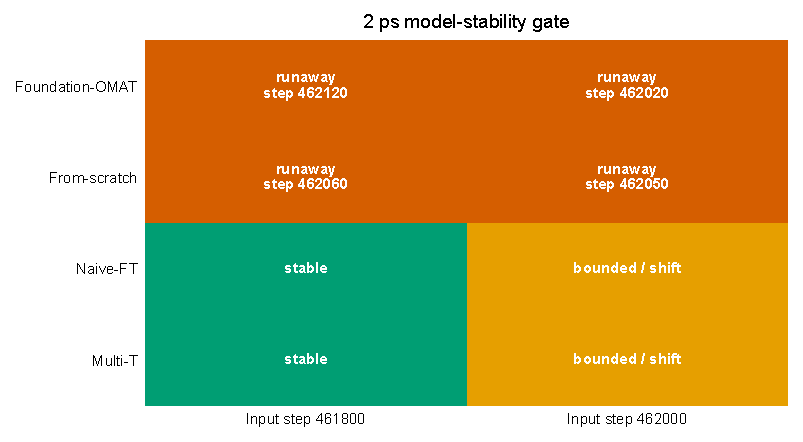
\includegraphics[width=\linewidth,height=0.42\textheight,keepaspectratio]{figure_pages/assets/fig_102.pdf}
\caption{Handoff molecular-dynamics diagnostics and first-divergence audit. This page shows the candidate output ``Phase2 stability gate'' within the audited P2-HANDOFF family. The panel identity, source scope, and current status are retained in the accompanying evidence matrix.}
\label{fig:candidate_102}
\end{figure}
\textbf{Results text draft.} The panels track the temperature, force, contact, and structural observables used to locate the first anomalous behavior after protocol handoff. Run-level integrity and local-neighborhood evidence are kept alongside the visualization.
\textbf{Discussion and boundary.} This is a diagnostic figure for identifying when and how trajectories depart from the accepted regime. It is not a replacement for a completed, gate-passing production trajectory.
\textbf{Article placement.} Proposed article location: Results: dynamic stability mechanism.
\textbf{Reviewer linkage:} overall status NO\_DIRECT\_REVIEWER\_FIGURE\_LINK.
No direct reviewer-response figure linkage was identified; this page is retained for scientific/article audit rather than as a direct reviewer response.
\textbf{Evidence pointers.}
\begin{itemize}[leftmargin=1.4em,noitemsep]
\item Data/processed: \begingroup\scriptsize\url{paper/analysis/phase2_handoff_md_20261002/audit_20261003/figures/figure_manifest.json}\endgroup
\item Data/processed: \begingroup\scriptsize\url{paper/analysis/phase2_handoff_md_20261002/audit_20261003/figures/plot_env.json}\endgroup
\item Plot/processing script: \begingroup\scriptsize\url{paper/analysis/phase2_handoff_md_20261002/audit_20261003/audit_phase2.py}\endgroup
\item Plot/processing script: \begingroup\scriptsize\url{paper/analysis/phase2_handoff_md_20261002/audit_20261003/extract_first_anomaly_remote.py}\endgroup
\item Caption/text source: \begingroup\scriptsize\url{paper/analysis/phase2_handoff_md_20261002/audit_20261003/PAPER_TEXT.md}\endgroup
\item Caption/text source: \begingroup\scriptsize\url{paper/analysis/phase2_handoff_md_20261002/audit_20261003/README.md}\endgroup
\end{itemize}
\statusline{\textbf{Audit gap / next action:} Duplicate checkout; reconcile against current package}
\vfill
\clearpage
\section{FIG-103 --- Handoff stability heatmap}
\label{figpage:fig-103}
\textbf{Group:} P2-HANDOFF\quad \textbf{Evidence chain:} traceable\quad \textbf{Status:} publication
\begin{figure}[H]
\centering
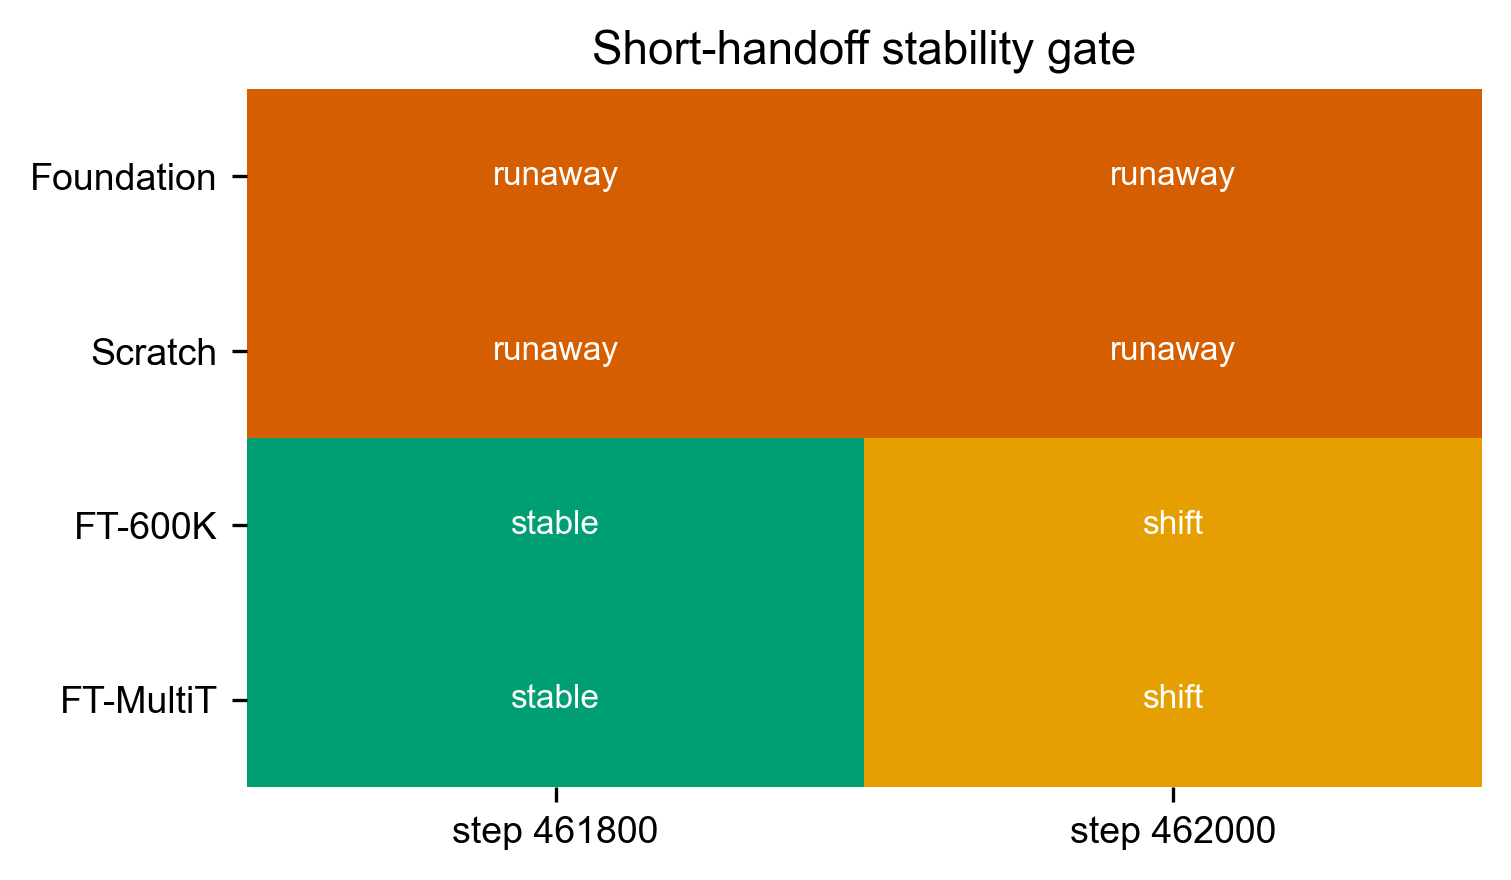
\includegraphics[width=\linewidth,height=0.42\textheight,keepaspectratio]{figure_pages/assets/fig_103.png}
\caption{Handoff molecular-dynamics diagnostics and first-divergence audit. This page shows the candidate output ``Handoff stability heatmap'' within the audited P2-HANDOFF family. The panel identity, source scope, and current status are retained in the accompanying evidence matrix.}
\label{fig:candidate_103}
\end{figure}
\textbf{Results text draft.} The panels track the temperature, force, contact, and structural observables used to locate the first anomalous behavior after protocol handoff. Run-level integrity and local-neighborhood evidence are kept alongside the visualization.
\textbf{Discussion and boundary.} This is a diagnostic figure for identifying when and how trajectories depart from the accepted regime. It is not a replacement for a completed, gate-passing production trajectory.
\textbf{Article placement.} Proposed article location: Results: dynamic stability mechanism.
\textbf{Reviewer linkage:} overall status NO\_DIRECT\_REVIEWER\_FIGURE\_LINK.
No direct reviewer-response figure linkage was identified; this page is retained for scientific/article audit rather than as a direct reviewer response.
\textbf{Evidence pointers.}
\begin{itemize}[leftmargin=1.4em,noitemsep]
\item Data/processed: \begingroup\scriptsize\url{paper/analysis/phase2_handoff_md_20261002/remote_artifacts/runs/retry2/stability_summary.csv}\endgroup
\item Data/processed: \begingroup\scriptsize\url{paper/analysis/phase2_handoff_md_20261002/remote_artifacts/runs/retry2/stability_summary.json}\endgroup
\end{itemize}
\statusline{\textbf{Audit gap / next action:} Duplicate checkout; reconcile against current package}
\vfill
\clearpage
\section{FIG-104 --- Handoff timeseries}
\label{figpage:fig-104}
\textbf{Group:} P2-HANDOFF\quad \textbf{Evidence chain:} traceable\quad \textbf{Status:} publication
\begin{figure}[H]
\centering
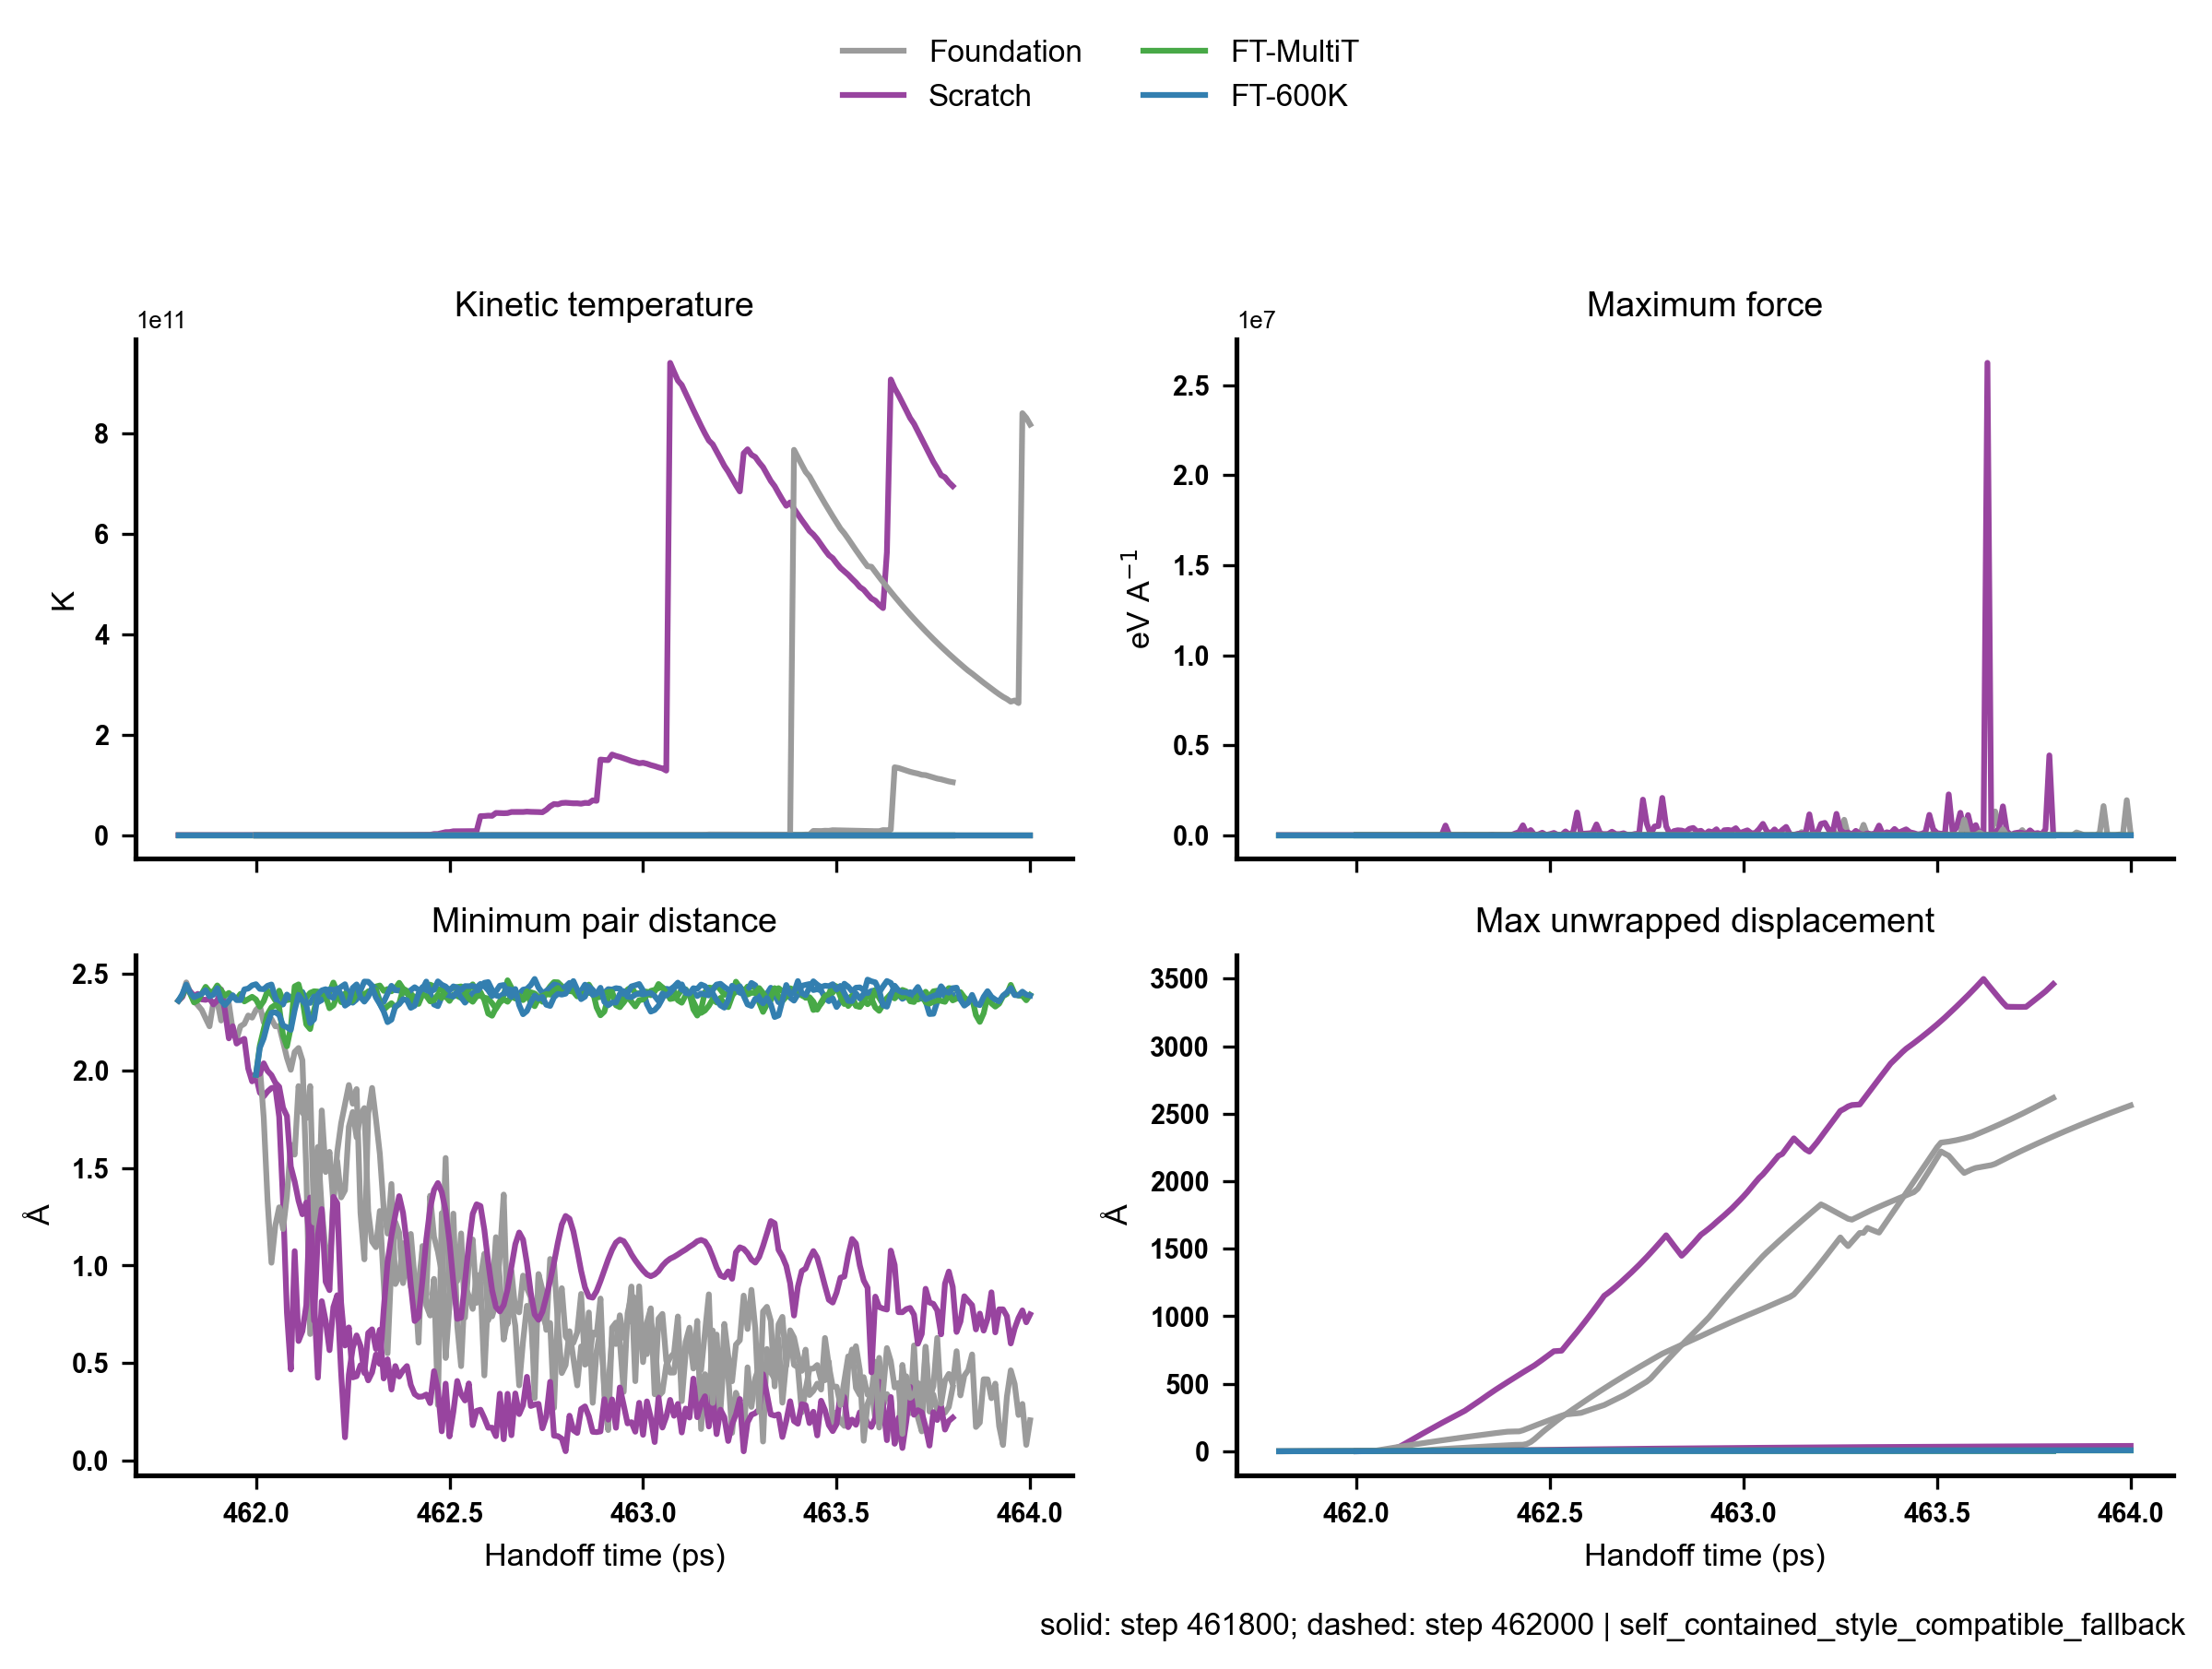
\includegraphics[width=\linewidth,height=0.42\textheight,keepaspectratio]{figure_pages/assets/fig_104.png}
\caption{Handoff molecular-dynamics diagnostics and first-divergence audit. This page shows the candidate output ``Handoff timeseries'' within the audited P2-HANDOFF family. The panel identity, source scope, and current status are retained in the accompanying evidence matrix.}
\label{fig:candidate_104}
\end{figure}
\textbf{Results text draft.} The panels track the temperature, force, contact, and structural observables used to locate the first anomalous behavior after protocol handoff. Run-level integrity and local-neighborhood evidence are kept alongside the visualization.
\textbf{Discussion and boundary.} This is a diagnostic figure for identifying when and how trajectories depart from the accepted regime. It is not a replacement for a completed, gate-passing production trajectory.
\textbf{Article placement.} Proposed article location: Results: dynamic stability mechanism.
\textbf{Reviewer linkage:} overall status NO\_DIRECT\_REVIEWER\_FIGURE\_LINK.
No direct reviewer-response figure linkage was identified; this page is retained for scientific/article audit rather than as a direct reviewer response.
\textbf{Evidence pointers.}
\begin{itemize}[leftmargin=1.4em,noitemsep]
\item Data/processed: \begingroup\scriptsize\url{paper/analysis/phase2_handoff_md_20261002/remote_artifacts/runs/retry2/stability_summary.csv}\endgroup
\item Data/processed: \begingroup\scriptsize\url{paper/analysis/phase2_handoff_md_20261002/remote_artifacts/runs/retry2/stability_summary.json}\endgroup
\end{itemize}
\statusline{\textbf{Audit gap / next action:} Duplicate checkout; reconcile against current package}
\vfill
\clearpage
\section{FIG-105 --- Mace reconstruction diagnostic}
\label{figpage:fig-105}
\textbf{Group:} P3-DFT\quad \textbf{Evidence chain:} partial\quad \textbf{Status:} exploratory;publication
\begin{figure}[H]
\centering
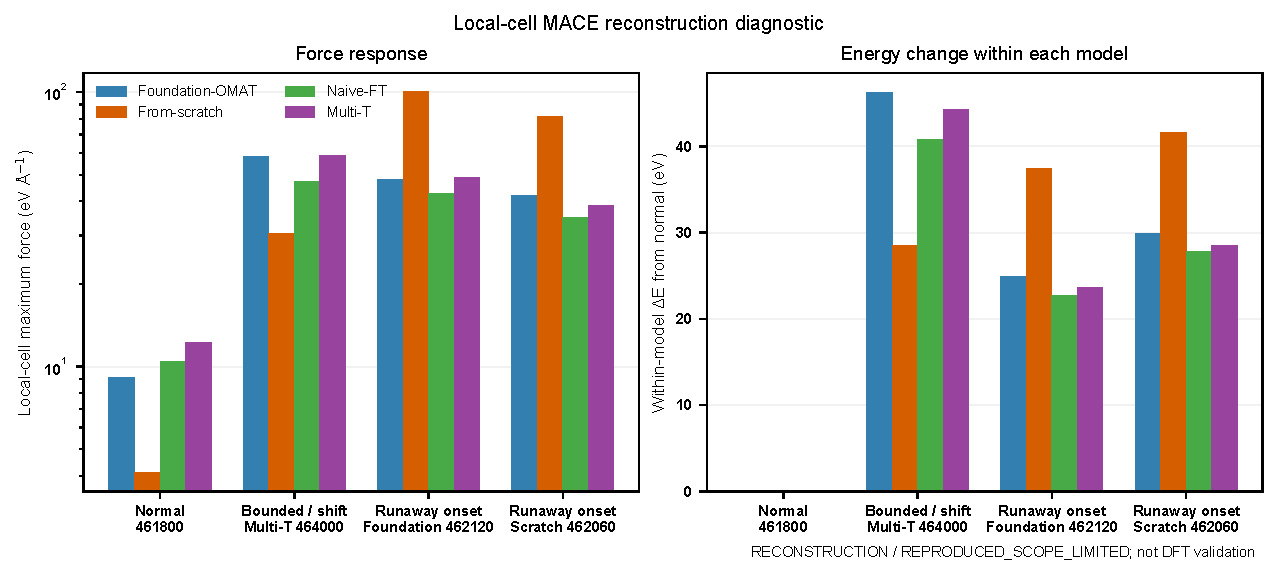
\includegraphics[width=\linewidth,height=0.42\textheight,keepaspectratio]{figure_pages/assets/fig_105.pdf}
\caption{Dft validation input, force, or candidate-quality audit. This page shows the candidate output ``Mace reconstruction diagnostic'' within the audited P3-DFT family. The panel identity, source scope, and current status are retained in the accompanying evidence matrix.}
\label{fig:candidate_105}
\end{figure}
\textbf{Results text draft.} The figure reports the audited state of the DFT validation inputs and the available force-level checks. Input identity, atom counts, ordering, and MACE/DFT scope are separated from claims about converged Quantum ESPRESSO output.
\textbf{Discussion and boundary.} Use to document readiness and failure boundaries. A finite MACE input audit or a submitted QE job is not itself an accepted DFT reference; convergence and normal termination remain required.
\textbf{Article placement.} Proposed article location: Results/SI: DFT gate and model-force validation.
\textbf{Reviewer linkage:} overall status PARTIAL.
\begin{itemize}[leftmargin=1.4em,noitemsep]
\item \textbf{REV-A1 (PARTIAL):} Reconcile Fig. 3d fixed-geometry DFT-path scoring with SI Fig. S3 self-consistent MLFF-NEB, including pathway identity and the DFT reference. \emph{Completed:} The fixed-path versus self-relaxed operator distinction and the narrower model-reported-barrier wording are integrated. \emph{Still required:} Close the restartable QE path-1--4 convergence gate, preserve the final path/source metadata, and complete the SI Fig. S3 endpoint/checkpoint/optimizer/source audit before calling the quantitative reference final.
\end{itemize}
\textbf{Evidence pointers.}
\begin{itemize}[leftmargin=1.4em,noitemsep]
\item Data/processed: \begingroup\scriptsize\url{paper/analysis/phase3_dft_recovery_20261004/mace_results/figures/figure_manifest.json}\endgroup
\item Data/processed: \begingroup\scriptsize\url{paper/analysis/phase3_dft_recovery_20261004/mace_results/figures/plot_env.json}\endgroup
\item Caption/text source: \begingroup\scriptsize\url{paper/analysis/phase3_dft_recovery_20261004/mace_results/MACE_RESULTS.md}\endgroup
\item Caption/text source: \begingroup\scriptsize\url{paper/analysis/phase3_dft_recovery_20261004/mace_results/slurm-31590216.out}\endgroup
\end{itemize}
\statusline{\textbf{Audit gap / next action:} No accepted formal DFT target is available in the audited state}
\vfill
\clearpage
\section{FIG-106 --- Mace force landscape step 462000 81}
\label{figpage:fig-106}
\textbf{Group:} P3-DFT\quad \textbf{Evidence chain:} partial\quad \textbf{Status:} publication
\begin{figure}[H]
\centering
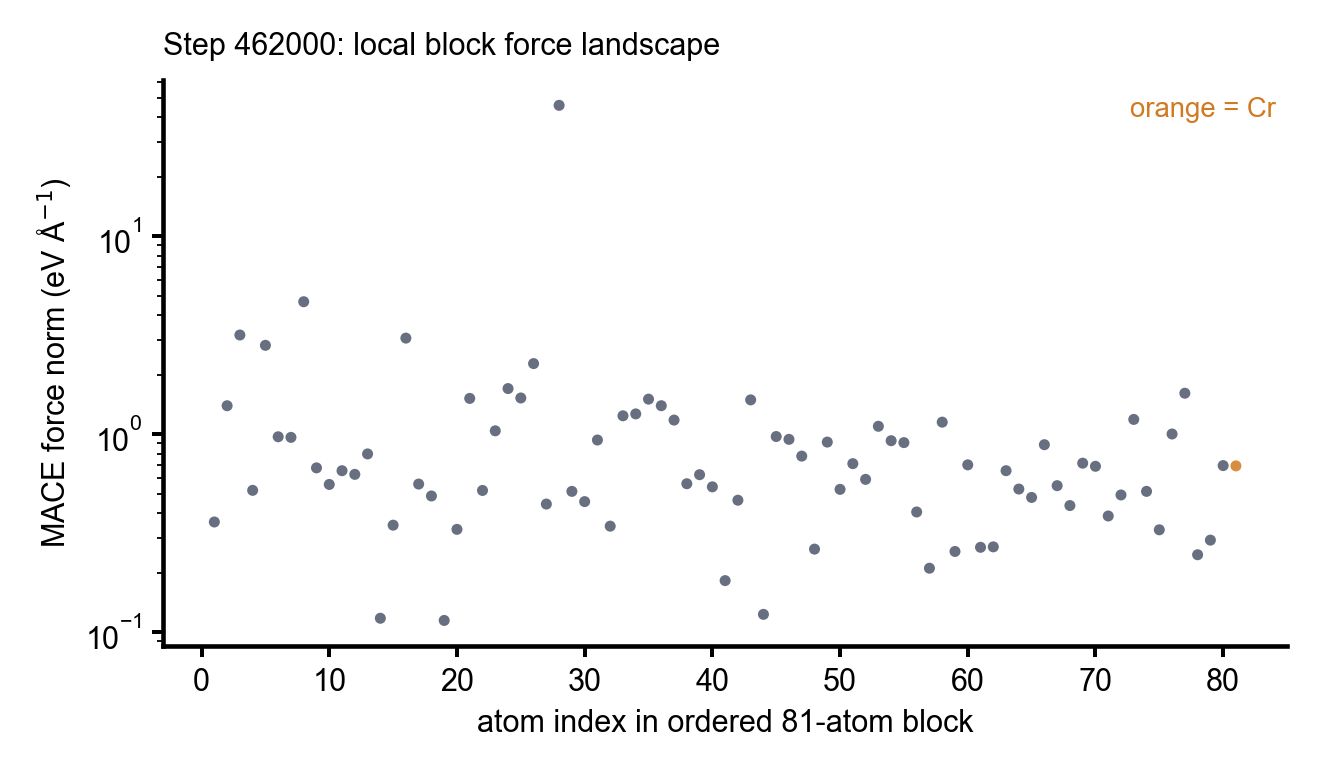
\includegraphics[width=\linewidth,height=0.42\textheight,keepaspectratio]{figure_pages/assets/fig_106.png}
\caption{Dft validation input, force, or candidate-quality audit. This page shows the candidate output ``Mace force landscape step 462000 81'' within the audited P3-DFT family. The panel identity, source scope, and current status are retained in the accompanying evidence matrix.}
\label{fig:candidate_106}
\end{figure}
\textbf{Results text draft.} The figure reports the audited state of the DFT validation inputs and the available force-level checks. Input identity, atom counts, ordering, and MACE/DFT scope are separated from claims about converged Quantum ESPRESSO output.
\textbf{Discussion and boundary.} Use to document readiness and failure boundaries. A finite MACE input audit or a submitted QE job is not itself an accepted DFT reference; convergence and normal termination remain required.
\textbf{Article placement.} Proposed article location: Results/SI: DFT gate and model-force validation.
\textbf{Reviewer linkage:} overall status PARTIAL.
\begin{itemize}[leftmargin=1.4em,noitemsep]
\item \textbf{REV-A1 (PARTIAL):} Reconcile Fig. 3d fixed-geometry DFT-path scoring with SI Fig. S3 self-consistent MLFF-NEB, including pathway identity and the DFT reference. \emph{Completed:} The fixed-path versus self-relaxed operator distinction and the narrower model-reported-barrier wording are integrated. \emph{Still required:} Close the restartable QE path-1--4 convergence gate, preserve the final path/source metadata, and complete the SI Fig. S3 endpoint/checkpoint/optimizer/source audit before calling the quantitative reference final.
\end{itemize}
\textbf{Evidence pointers.}
\begin{itemize}[leftmargin=1.4em,noitemsep]
\item Data/processed: \begingroup\scriptsize\url{paper/analysis/phase3_dft_validation_20261002/job_ledger.csv}\endgroup
\item Data/processed: \begingroup\scriptsize\url{paper/analysis/phase3_dft_validation_20261002/ordered_block_audit.csv}\endgroup
\item Caption/text source: \begingroup\scriptsize\url{paper/analysis/phase3_dft_validation_20261002/README.md}\endgroup
\item Caption/text source: \begingroup\scriptsize\url{paper/analysis/phase3_dft_validation_20261002/manager_recommendation.md}\endgroup
\end{itemize}
\statusline{\textbf{Audit gap / next action:} No accepted formal DFT target is available in the audited state}
\vfill
\clearpage
\section{FIG-107 --- Mace force progression 81}
\label{figpage:fig-107}
\textbf{Group:} P3-DFT\quad \textbf{Evidence chain:} partial\quad \textbf{Status:} publication
\begin{figure}[H]
\centering
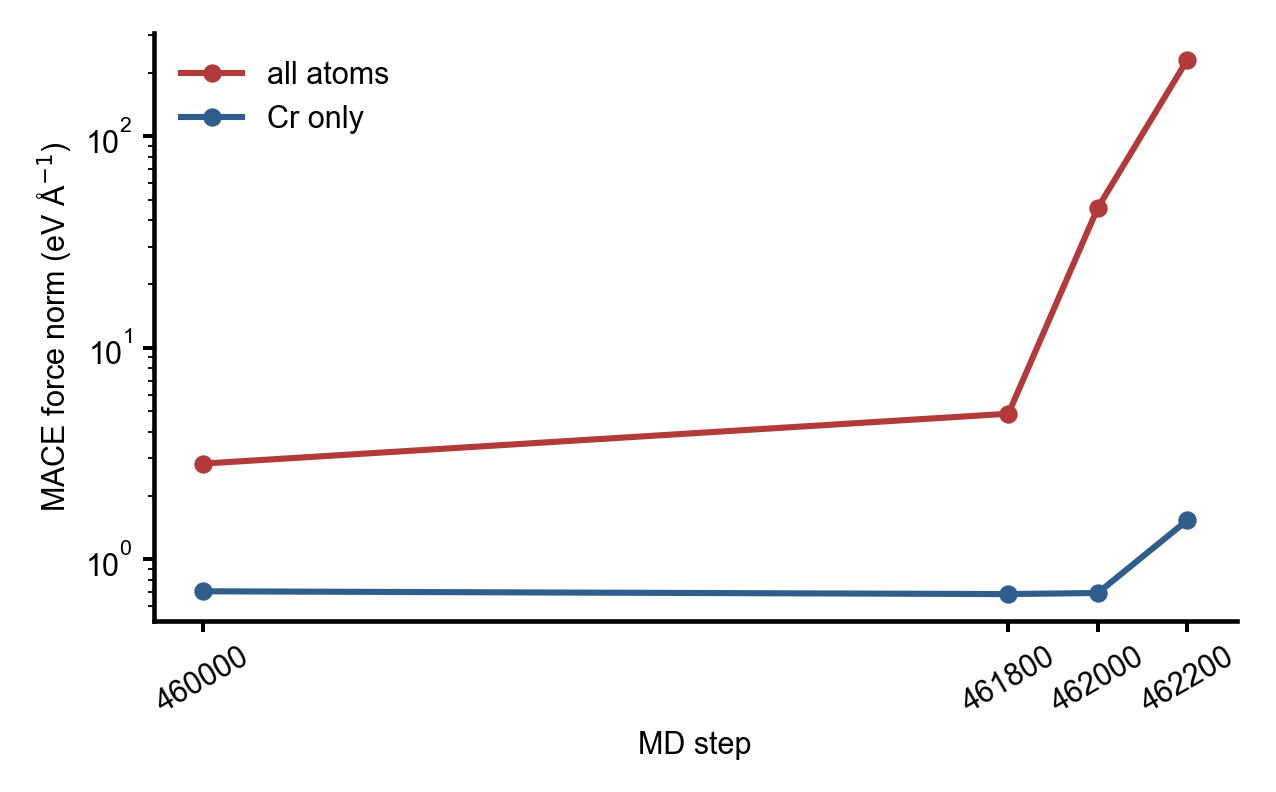
\includegraphics[width=\linewidth,height=0.42\textheight,keepaspectratio]{figure_pages/assets/fig_107.png}
\caption{Dft validation input, force, or candidate-quality audit. This page shows the candidate output ``Mace force progression 81'' within the audited P3-DFT family. The panel identity, source scope, and current status are retained in the accompanying evidence matrix.}
\label{fig:candidate_107}
\end{figure}
\textbf{Results text draft.} The figure reports the audited state of the DFT validation inputs and the available force-level checks. Input identity, atom counts, ordering, and MACE/DFT scope are separated from claims about converged Quantum ESPRESSO output.
\textbf{Discussion and boundary.} Use to document readiness and failure boundaries. A finite MACE input audit or a submitted QE job is not itself an accepted DFT reference; convergence and normal termination remain required.
\textbf{Article placement.} Proposed article location: Results/SI: DFT gate and model-force validation.
\textbf{Reviewer linkage:} overall status PARTIAL.
\begin{itemize}[leftmargin=1.4em,noitemsep]
\item \textbf{REV-A1 (PARTIAL):} Reconcile Fig. 3d fixed-geometry DFT-path scoring with SI Fig. S3 self-consistent MLFF-NEB, including pathway identity and the DFT reference. \emph{Completed:} The fixed-path versus self-relaxed operator distinction and the narrower model-reported-barrier wording are integrated. \emph{Still required:} Close the restartable QE path-1--4 convergence gate, preserve the final path/source metadata, and complete the SI Fig. S3 endpoint/checkpoint/optimizer/source audit before calling the quantitative reference final.
\end{itemize}
\textbf{Evidence pointers.}
\begin{itemize}[leftmargin=1.4em,noitemsep]
\item Data/processed: \begingroup\scriptsize\url{paper/analysis/phase3_dft_validation_20261002/job_ledger.csv}\endgroup
\item Data/processed: \begingroup\scriptsize\url{paper/analysis/phase3_dft_validation_20261002/ordered_block_audit.csv}\endgroup
\item Caption/text source: \begingroup\scriptsize\url{paper/analysis/phase3_dft_validation_20261002/README.md}\endgroup
\item Caption/text source: \begingroup\scriptsize\url{paper/analysis/phase3_dft_validation_20261002/manager_recommendation.md}\endgroup
\end{itemize}
\statusline{\textbf{Audit gap / next action:} No accepted formal DFT target is available in the audited state}
\vfill
\clearpage
\section{FIG-108 --- Force relaxation curves}
\label{figpage:fig-108}
\textbf{Group:} ARCHIVE-ENDPOINT\quad \textbf{Evidence chain:} partial\quad \textbf{Status:} publication;comparison
\begin{figure}[H]
\centering
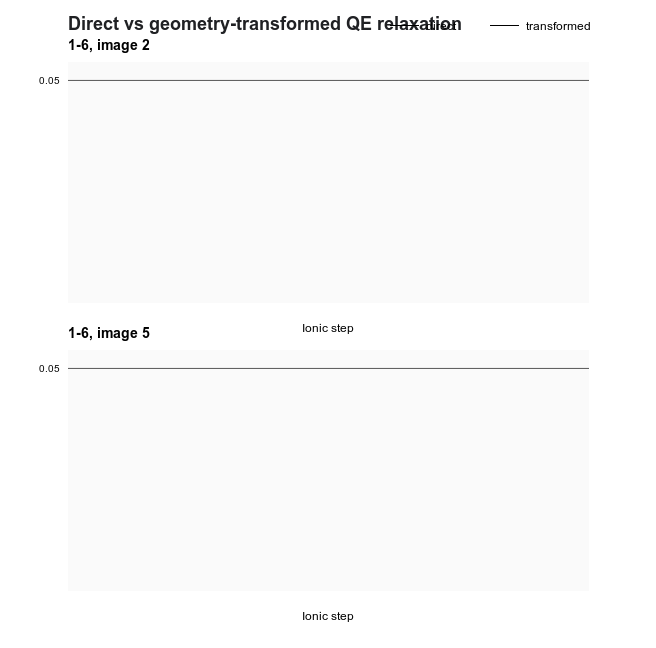
\includegraphics[width=\linewidth,height=0.42\textheight,keepaspectratio]{figure_pages/assets/fig_108.png}
\caption{Archived endpoint-relaxation or endpoint-quality evidence. This page shows the candidate output ``Force relaxation curves'' within the audited ARCHIVE-ENDPOINT family. The panel identity, source scope, and current status are retained in the accompanying evidence matrix.}
\label{fig:candidate_108}
\end{figure}
\textbf{Results text draft.} The figure preserves endpoint candidates and their quality flags as an auditable historical record. Endpoint stability is reported separately from path and transition-state validity.
\textbf{Discussion and boundary.} Use for provenance and candidate selection. Endpoints alone cannot validate a migration barrier or a complete NEB pathway.
\textbf{Article placement.} Proposed article location: SI endpoint-relaxation evidence.
\textbf{Reviewer linkage:} overall status NO\_DIRECT\_REVIEWER\_FIGURE\_LINK.
No direct reviewer-response figure linkage was identified; this page is retained for scientific/article audit rather than as a direct reviewer response.
\textbf{Evidence pointers.}
\begin{itemize}[leftmargin=1.4em,noitemsep]
\item Data/processed: \begingroup\scriptsize\url{paper/data/published/endpoint_relax_comparison/exact_iter/1-6_iter108/paired_relaxation_comparison.csv}\endgroup
\item Data/processed: \begingroup\scriptsize\url{paper/data/published/endpoint_relax_comparison/exact_iter/1-6_iter108/paired_relaxation_comparison.json}\endgroup
\item Caption/text source: \begingroup\scriptsize\url{paper/data/published/endpoint_relax_comparison/exact_iter/1-6_iter108/README.md}\endgroup
\end{itemize}
\statusline{\textbf{Audit gap / next action:} Recover generator and exact raw log lineage}
\vfill
\clearpage
\section{FIG-109 --- Force relaxation curves}
\label{figpage:fig-109}
\textbf{Group:} ARCHIVE-ENDPOINT\quad \textbf{Evidence chain:} partial\quad \textbf{Status:} publication;comparison
\begin{figure}[H]
\centering
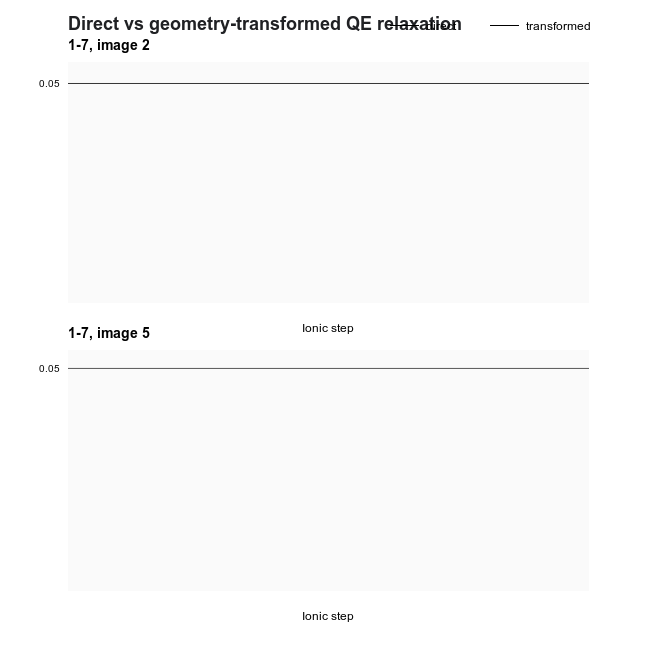
\includegraphics[width=\linewidth,height=0.42\textheight,keepaspectratio]{figure_pages/assets/fig_109.png}
\caption{Archived endpoint-relaxation or endpoint-quality evidence. This page shows the candidate output ``Force relaxation curves'' within the audited ARCHIVE-ENDPOINT family. The panel identity, source scope, and current status are retained in the accompanying evidence matrix.}
\label{fig:candidate_109}
\end{figure}
\textbf{Results text draft.} The figure preserves endpoint candidates and their quality flags as an auditable historical record. Endpoint stability is reported separately from path and transition-state validity.
\textbf{Discussion and boundary.} Use for provenance and candidate selection. Endpoints alone cannot validate a migration barrier or a complete NEB pathway.
\textbf{Article placement.} Proposed article location: SI endpoint-relaxation evidence.
\textbf{Reviewer linkage:} overall status NO\_DIRECT\_REVIEWER\_FIGURE\_LINK.
No direct reviewer-response figure linkage was identified; this page is retained for scientific/article audit rather than as a direct reviewer response.
\textbf{Evidence pointers.}
\begin{itemize}[leftmargin=1.4em,noitemsep]
\item Data/processed: \begingroup\scriptsize\url{paper/data/published/endpoint_relax_comparison/exact_iter/1-7_iter112/paired_relaxation_comparison.csv}\endgroup
\item Data/processed: \begingroup\scriptsize\url{paper/data/published/endpoint_relax_comparison/exact_iter/1-7_iter112/paired_relaxation_comparison.json}\endgroup
\item Caption/text source: \begingroup\scriptsize\url{paper/data/published/endpoint_relax_comparison/exact_iter/1-7_iter112/README.md}\endgroup
\end{itemize}
\statusline{\textbf{Audit gap / next action:} Recover generator and exact raw log lineage}
\vfill
\clearpage
\section{FIG-110 --- Foundation self neb rescored profile}
\label{figpage:fig-110}
\textbf{Group:} ARCHIVE-SELFNEB\quad \textbf{Evidence chain:} partial\quad \textbf{Status:} publication;old\_or\_legacy;audit
\begin{figure}[H]
\centering
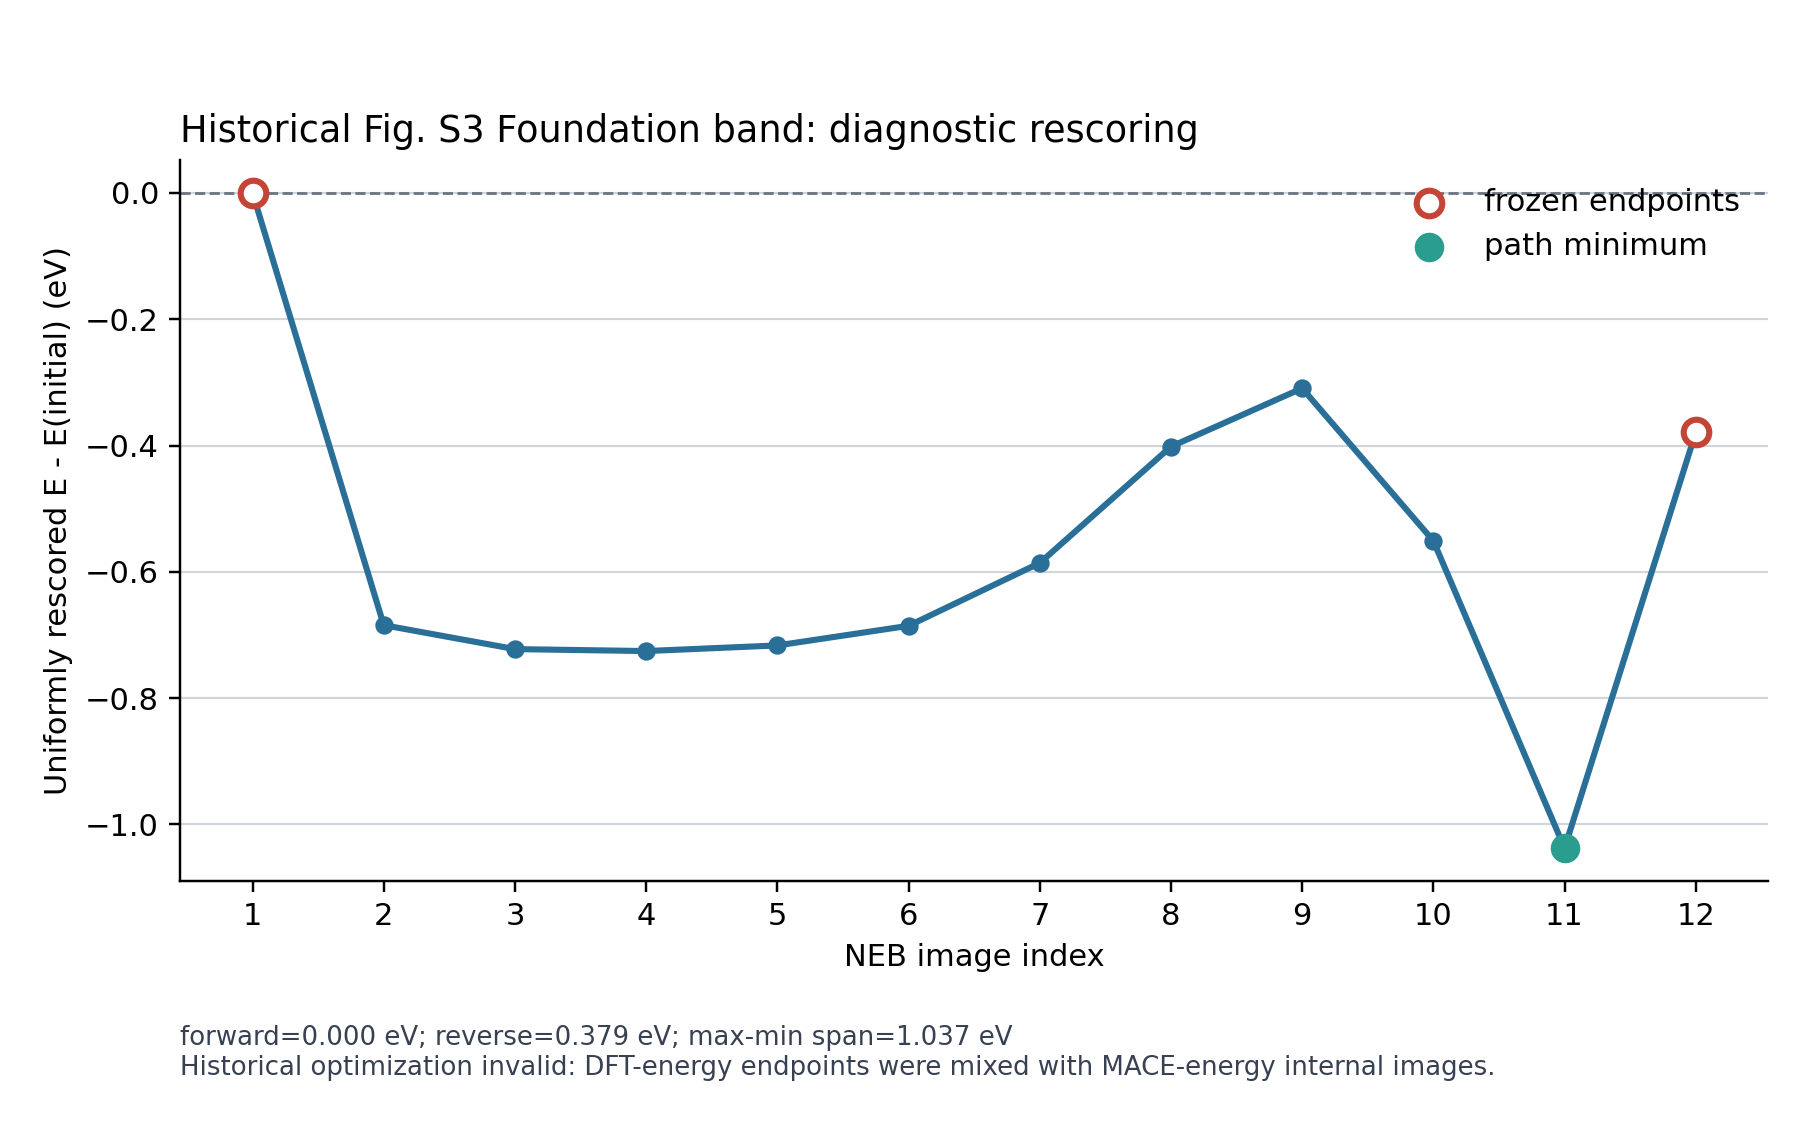
\includegraphics[width=\linewidth,height=0.42\textheight,keepaspectratio]{figure_pages/assets/fig_110.png}
\caption{Archived self-consistent mlff-neb evidence. This page shows the candidate output ``Foundation self neb rescored profile'' within the audited ARCHIVE-SELFNEB family. The panel identity, source scope, and current status are retained in the accompanying evidence matrix.}
\label{fig:candidate_110}
\end{figure}
\textbf{Results text draft.} The figure records the available model-relaxed NEB behavior and separates convergence from instability. The reported barrier, when present, is a model-reported value on that model's own optimized band.
\textbf{Discussion and boundary.} This supports the narrower claim of self-consistent path-generation stability. It is not interchangeable with fixed-geometry DFT-path scoring.
\textbf{Article placement.} Proposed article location: SI NEB stability audit.
\textbf{Reviewer linkage:} overall status PARTIAL.
\begin{itemize}[leftmargin=1.4em,noitemsep]
\item \textbf{REV-A1 (PARTIAL):} Reconcile Fig. 3d fixed-geometry DFT-path scoring with SI Fig. S3 self-consistent MLFF-NEB, including pathway identity and the DFT reference. \emph{Completed:} The fixed-path versus self-relaxed operator distinction and the narrower model-reported-barrier wording are integrated. \emph{Still required:} Close the restartable QE path-1--4 convergence gate, preserve the final path/source metadata, and complete the SI Fig. S3 endpoint/checkpoint/optimizer/source audit before calling the quantitative reference final.
\end{itemize}
\textbf{Evidence pointers.}
No data/script/text candidate was recorded in the matrix; resolve this gap before manuscript promotion.
\statusline{\textbf{Audit gap / next action:} Source input and renderer are not co-located}
\vfill
\clearpage
\section{FIG-111 --- Mlff preconditioner residual}
\label{figpage:fig-111}
\textbf{Group:} ARCHIVE-PRECOND\quad \textbf{Evidence chain:} partial\quad \textbf{Status:} publication;old\_or\_legacy;audit;comparison
\begin{figure}[H]
\centering
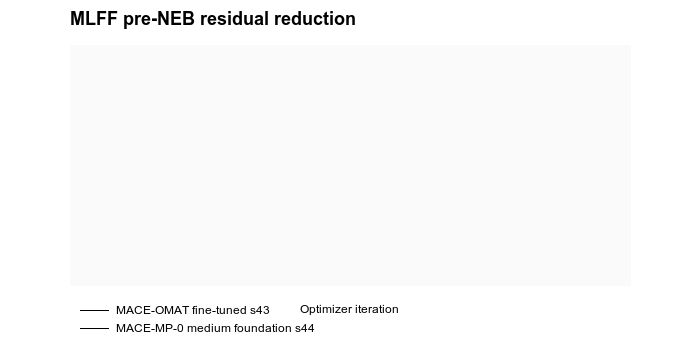
\includegraphics[width=\linewidth,height=0.42\textheight,keepaspectratio]{figure_pages/assets/fig_111.png}
\caption{Archived calculation precondition or readiness audit. This page shows the candidate output ``Mlff preconditioner residual'' within the audited ARCHIVE-PRECOND family. The panel identity, source scope, and current status are retained in the accompanying evidence matrix.}
\label{fig:candidate_111}
\end{figure}
\textbf{Results text draft.} The figure summarizes the preconditions checked before a calculation was eligible for interpretation. Missing or failed prerequisites remain explicit.
\textbf{Discussion and boundary.} Use as a methods/audit figure rather than as a scientific result. Readiness does not substitute for a completed accepted calculation.
\textbf{Article placement.} Proposed article location: SI NEB methods/audit.
\textbf{Reviewer linkage:} overall status NO\_DIRECT\_REVIEWER\_FIGURE\_LINK.
No direct reviewer-response figure linkage was identified; this page is retained for scientific/article audit rather than as a direct reviewer response.
\textbf{Evidence pointers.}
\begin{itemize}[leftmargin=1.4em,noitemsep]
\item Data/processed: \begingroup\scriptsize\url{paper/data/published/mlff_preconditioner_comparison/nonlinear_historical_warp_smoke/mlff_preconditioner_comparison.csv}\endgroup
\item Data/processed: \begingroup\scriptsize\url{paper/data/published/mlff_preconditioner_comparison/nonlinear_historical_warp_smoke/mlff_preconditioner_comparison.json}\endgroup
\end{itemize}
\statusline{\textbf{Audit gap / next action:} Recover source path and plotting command}
\vfill
\clearpage
\section{FIG-112 --- 1 2 historical}
\label{figpage:fig-112}
\textbf{Group:} ARCHIVE-NEB-BARRIER\quad \textbf{Evidence chain:} partial\quad \textbf{Status:} publication;old\_or\_legacy
\begin{figure}[H]
\centering
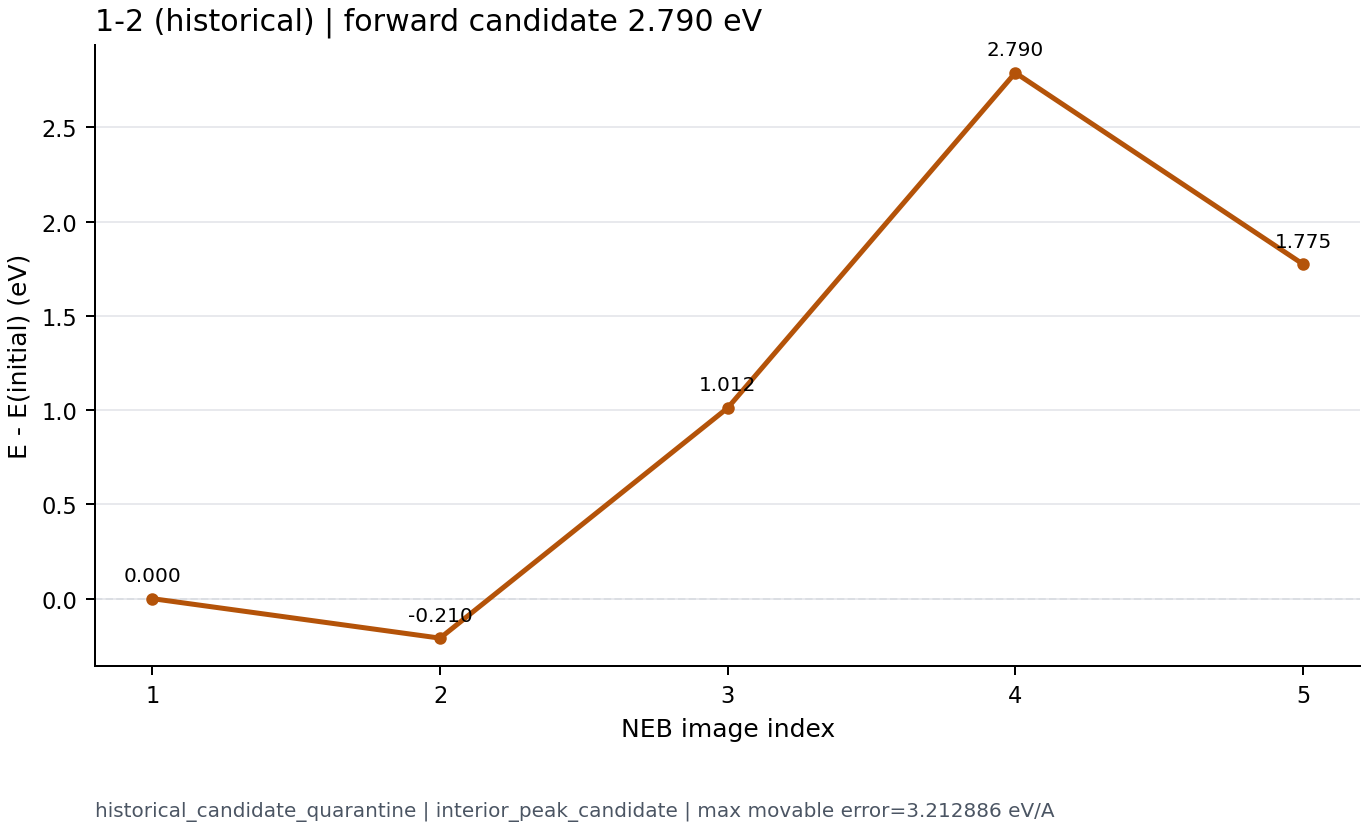
\includegraphics[width=\linewidth,height=0.42\textheight,keepaspectratio]{figure_pages/assets/fig_112.png}
\caption{Archived neb barrier inventory with convergence and provenance flags. This page shows the candidate output ``1 2 historical'' within the audited ARCHIVE-NEB-BARRIER family. The panel identity, source scope, and current status are retained in the accompanying evidence matrix.}
\label{fig:candidate_112}
\end{figure}
\textbf{Results text draft.} The bars or points retain candidate, unconverged, diverged, and accepted statuses rather than collapsing them into one ranking. Barrier values are interpreted only together with path identity and convergence metadata.
\textbf{Discussion and boundary.} Only rows that satisfy the final convergence criterion may serve as quantitative reference values. The remaining entries are useful for audit history and restart planning.
\textbf{Article placement.} Proposed article location: SI DFT NEB barrier inventory.
\textbf{Reviewer linkage:} overall status PARTIAL.
\begin{itemize}[leftmargin=1.4em,noitemsep]
\item \textbf{REV-A1 (PARTIAL):} Reconcile Fig. 3d fixed-geometry DFT-path scoring with SI Fig. S3 self-consistent MLFF-NEB, including pathway identity and the DFT reference. \emph{Completed:} The fixed-path versus self-relaxed operator distinction and the narrower model-reported-barrier wording are integrated. \emph{Still required:} Close the restartable QE path-1--4 convergence gate, preserve the final path/source metadata, and complete the SI Fig. S3 endpoint/checkpoint/optimizer/source audit before calling the quantitative reference final.
\end{itemize}
\textbf{Evidence pointers.}
\begin{itemize}[leftmargin=1.4em,noitemsep]
\item Data/processed: \begingroup\scriptsize\url{paper/data/published/neb_barrier_atlas/barrier_atlas.csv}\endgroup
\item Data/processed: \begingroup\scriptsize\url{paper/data/published/neb_barrier_atlas/barrier_atlas.json}\endgroup
\item Caption/text source: \begingroup\scriptsize\url{paper/data/published/neb_barrier_atlas/README.md}\endgroup
\end{itemize}
\statusline{\textbf{Audit gap / next action:} No co-located plotting script; treat as archived derivative until source is recovered}
\vfill
\clearpage
\section{FIG-113 --- 1 3 historical}
\label{figpage:fig-113}
\textbf{Group:} ARCHIVE-NEB-BARRIER\quad \textbf{Evidence chain:} partial\quad \textbf{Status:} publication;old\_or\_legacy
\begin{figure}[H]
\centering
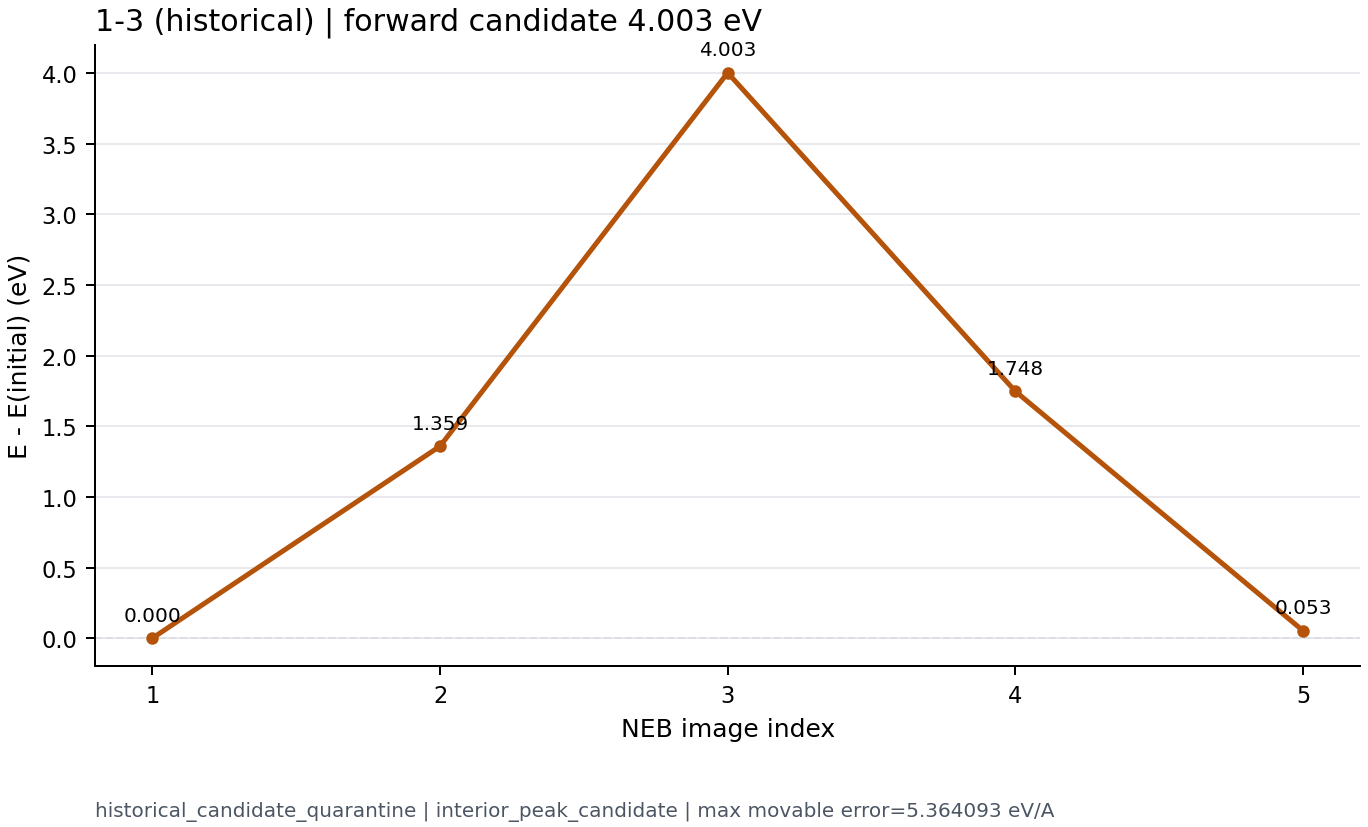
\includegraphics[width=\linewidth,height=0.42\textheight,keepaspectratio]{figure_pages/assets/fig_113.png}
\caption{Archived neb barrier inventory with convergence and provenance flags. This page shows the candidate output ``1 3 historical'' within the audited ARCHIVE-NEB-BARRIER family. The panel identity, source scope, and current status are retained in the accompanying evidence matrix.}
\label{fig:candidate_113}
\end{figure}
\textbf{Results text draft.} The bars or points retain candidate, unconverged, diverged, and accepted statuses rather than collapsing them into one ranking. Barrier values are interpreted only together with path identity and convergence metadata.
\textbf{Discussion and boundary.} Only rows that satisfy the final convergence criterion may serve as quantitative reference values. The remaining entries are useful for audit history and restart planning.
\textbf{Article placement.} Proposed article location: SI DFT NEB barrier inventory.
\textbf{Reviewer linkage:} overall status PARTIAL.
\begin{itemize}[leftmargin=1.4em,noitemsep]
\item \textbf{REV-A1 (PARTIAL):} Reconcile Fig. 3d fixed-geometry DFT-path scoring with SI Fig. S3 self-consistent MLFF-NEB, including pathway identity and the DFT reference. \emph{Completed:} The fixed-path versus self-relaxed operator distinction and the narrower model-reported-barrier wording are integrated. \emph{Still required:} Close the restartable QE path-1--4 convergence gate, preserve the final path/source metadata, and complete the SI Fig. S3 endpoint/checkpoint/optimizer/source audit before calling the quantitative reference final.
\end{itemize}
\textbf{Evidence pointers.}
\begin{itemize}[leftmargin=1.4em,noitemsep]
\item Data/processed: \begingroup\scriptsize\url{paper/data/published/neb_barrier_atlas/barrier_atlas.csv}\endgroup
\item Data/processed: \begingroup\scriptsize\url{paper/data/published/neb_barrier_atlas/barrier_atlas.json}\endgroup
\item Caption/text source: \begingroup\scriptsize\url{paper/data/published/neb_barrier_atlas/README.md}\endgroup
\end{itemize}
\statusline{\textbf{Audit gap / next action:} No co-located plotting script; treat as archived derivative until source is recovered}
\vfill
\clearpage
\section{FIG-114 --- 1 4 historical}
\label{figpage:fig-114}
\textbf{Group:} ARCHIVE-NEB-BARRIER\quad \textbf{Evidence chain:} partial\quad \textbf{Status:} publication;old\_or\_legacy
\begin{figure}[H]
\centering
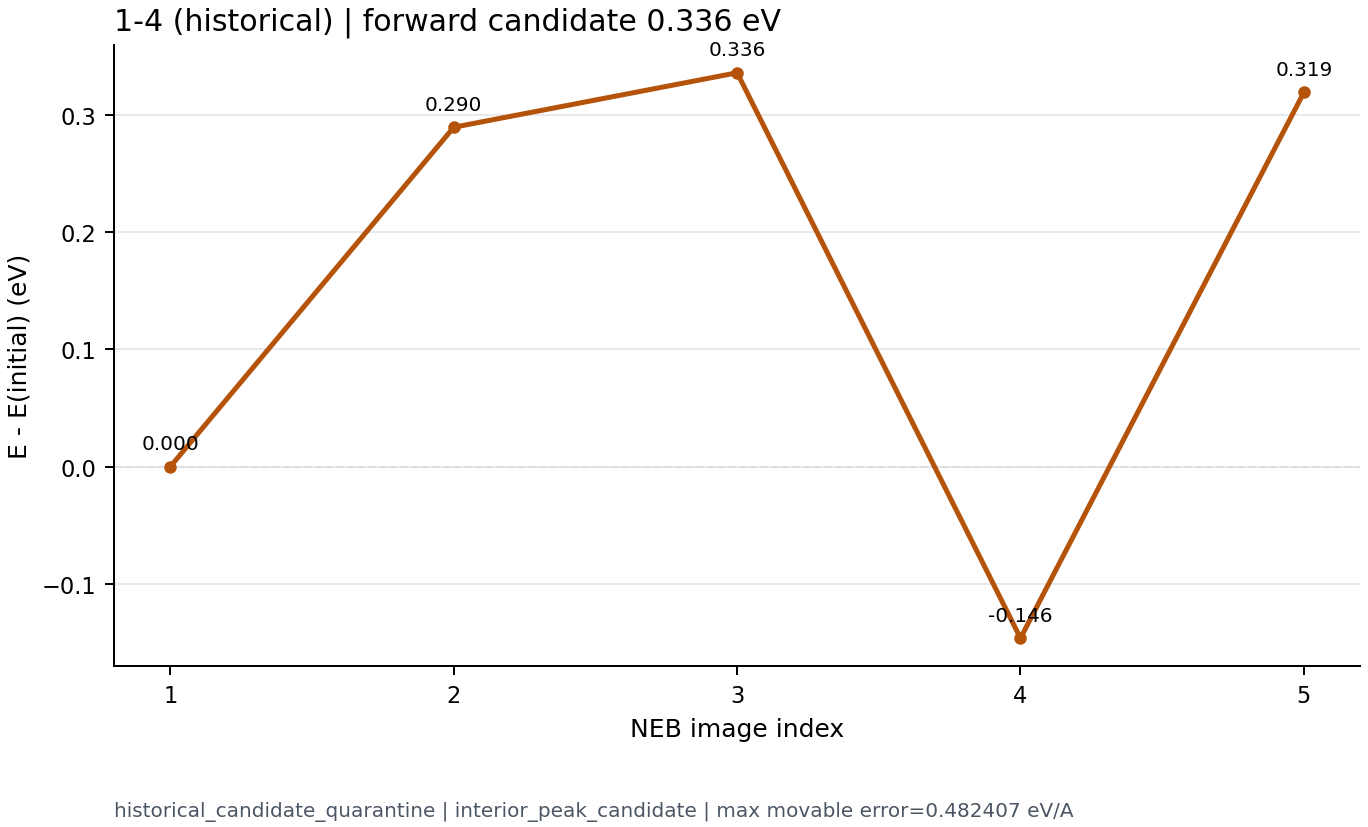
\includegraphics[width=\linewidth,height=0.42\textheight,keepaspectratio]{figure_pages/assets/fig_114.png}
\caption{Archived neb barrier inventory with convergence and provenance flags. This page shows the candidate output ``1 4 historical'' within the audited ARCHIVE-NEB-BARRIER family. The panel identity, source scope, and current status are retained in the accompanying evidence matrix.}
\label{fig:candidate_114}
\end{figure}
\textbf{Results text draft.} The bars or points retain candidate, unconverged, diverged, and accepted statuses rather than collapsing them into one ranking. Barrier values are interpreted only together with path identity and convergence metadata.
\textbf{Discussion and boundary.} Only rows that satisfy the final convergence criterion may serve as quantitative reference values. The remaining entries are useful for audit history and restart planning.
\textbf{Article placement.} Proposed article location: SI DFT NEB barrier inventory.
\textbf{Reviewer linkage:} overall status PARTIAL.
\begin{itemize}[leftmargin=1.4em,noitemsep]
\item \textbf{REV-A1 (PARTIAL):} Reconcile Fig. 3d fixed-geometry DFT-path scoring with SI Fig. S3 self-consistent MLFF-NEB, including pathway identity and the DFT reference. \emph{Completed:} The fixed-path versus self-relaxed operator distinction and the narrower model-reported-barrier wording are integrated. \emph{Still required:} Close the restartable QE path-1--4 convergence gate, preserve the final path/source metadata, and complete the SI Fig. S3 endpoint/checkpoint/optimizer/source audit before calling the quantitative reference final.
\end{itemize}
\textbf{Evidence pointers.}
\begin{itemize}[leftmargin=1.4em,noitemsep]
\item Data/processed: \begingroup\scriptsize\url{paper/data/published/neb_barrier_atlas/barrier_atlas.csv}\endgroup
\item Data/processed: \begingroup\scriptsize\url{paper/data/published/neb_barrier_atlas/barrier_atlas.json}\endgroup
\item Caption/text source: \begingroup\scriptsize\url{paper/data/published/neb_barrier_atlas/README.md}\endgroup
\end{itemize}
\statusline{\textbf{Audit gap / next action:} No co-located plotting script; treat as archived derivative until source is recovered}
\vfill
\clearpage
\section{FIG-115 --- 1 5 historical}
\label{figpage:fig-115}
\textbf{Group:} ARCHIVE-NEB-BARRIER\quad \textbf{Evidence chain:} partial\quad \textbf{Status:} publication;old\_or\_legacy
\begin{figure}[H]
\centering
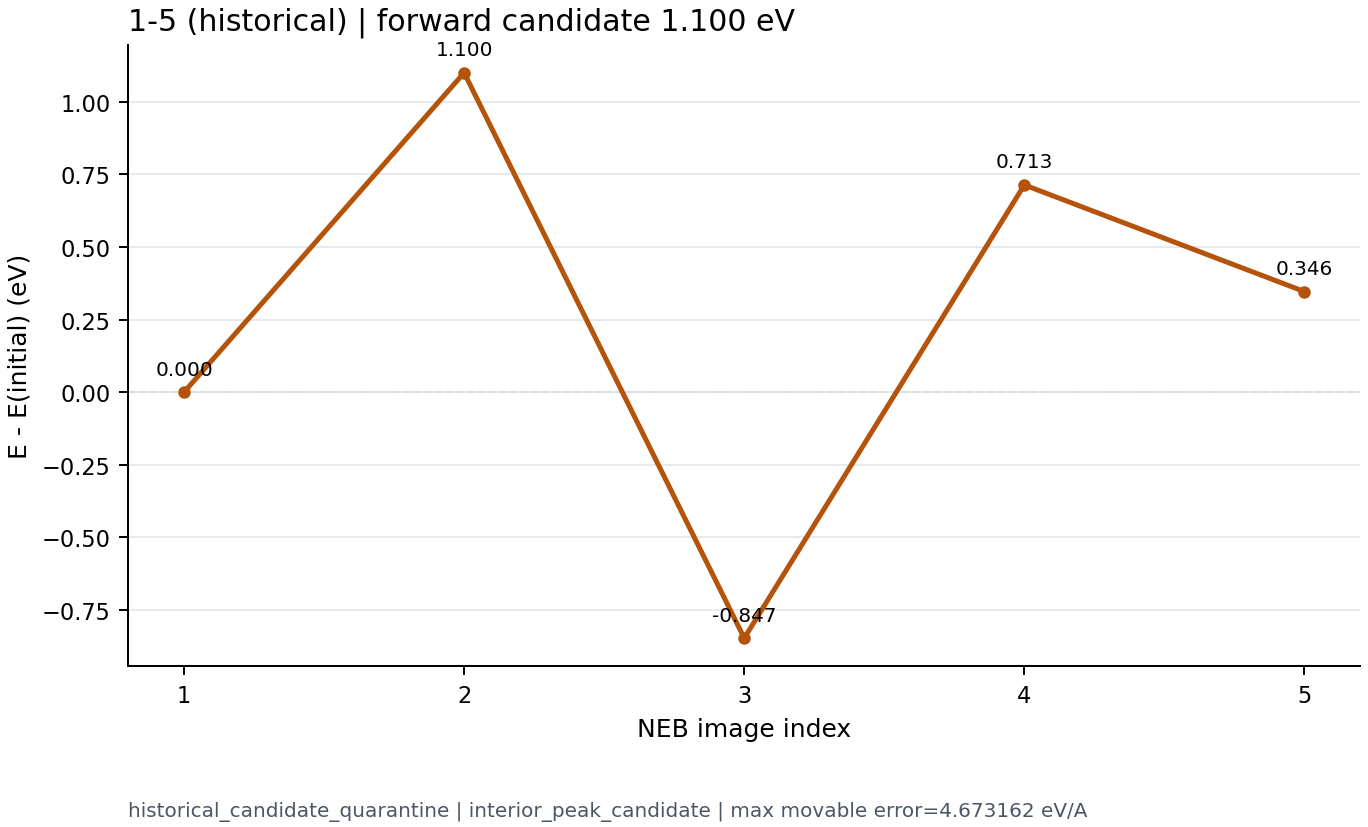
\includegraphics[width=\linewidth,height=0.42\textheight,keepaspectratio]{figure_pages/assets/fig_115.png}
\caption{Archived neb barrier inventory with convergence and provenance flags. This page shows the candidate output ``1 5 historical'' within the audited ARCHIVE-NEB-BARRIER family. The panel identity, source scope, and current status are retained in the accompanying evidence matrix.}
\label{fig:candidate_115}
\end{figure}
\textbf{Results text draft.} The bars or points retain candidate, unconverged, diverged, and accepted statuses rather than collapsing them into one ranking. Barrier values are interpreted only together with path identity and convergence metadata.
\textbf{Discussion and boundary.} Only rows that satisfy the final convergence criterion may serve as quantitative reference values. The remaining entries are useful for audit history and restart planning.
\textbf{Article placement.} Proposed article location: SI DFT NEB barrier inventory.
\textbf{Reviewer linkage:} overall status PARTIAL.
\begin{itemize}[leftmargin=1.4em,noitemsep]
\item \textbf{REV-A1 (PARTIAL):} Reconcile Fig. 3d fixed-geometry DFT-path scoring with SI Fig. S3 self-consistent MLFF-NEB, including pathway identity and the DFT reference. \emph{Completed:} The fixed-path versus self-relaxed operator distinction and the narrower model-reported-barrier wording are integrated. \emph{Still required:} Close the restartable QE path-1--4 convergence gate, preserve the final path/source metadata, and complete the SI Fig. S3 endpoint/checkpoint/optimizer/source audit before calling the quantitative reference final.
\end{itemize}
\textbf{Evidence pointers.}
\begin{itemize}[leftmargin=1.4em,noitemsep]
\item Data/processed: \begingroup\scriptsize\url{paper/data/published/neb_barrier_atlas/barrier_atlas.csv}\endgroup
\item Data/processed: \begingroup\scriptsize\url{paper/data/published/neb_barrier_atlas/barrier_atlas.json}\endgroup
\item Caption/text source: \begingroup\scriptsize\url{paper/data/published/neb_barrier_atlas/README.md}\endgroup
\end{itemize}
\statusline{\textbf{Audit gap / next action:} No co-located plotting script; treat as archived derivative until source is recovered}
\vfill
\clearpage
\section{FIG-116 --- 1 6 historical}
\label{figpage:fig-116}
\textbf{Group:} ARCHIVE-NEB-BARRIER\quad \textbf{Evidence chain:} partial\quad \textbf{Status:} publication;old\_or\_legacy
\begin{figure}[H]
\centering
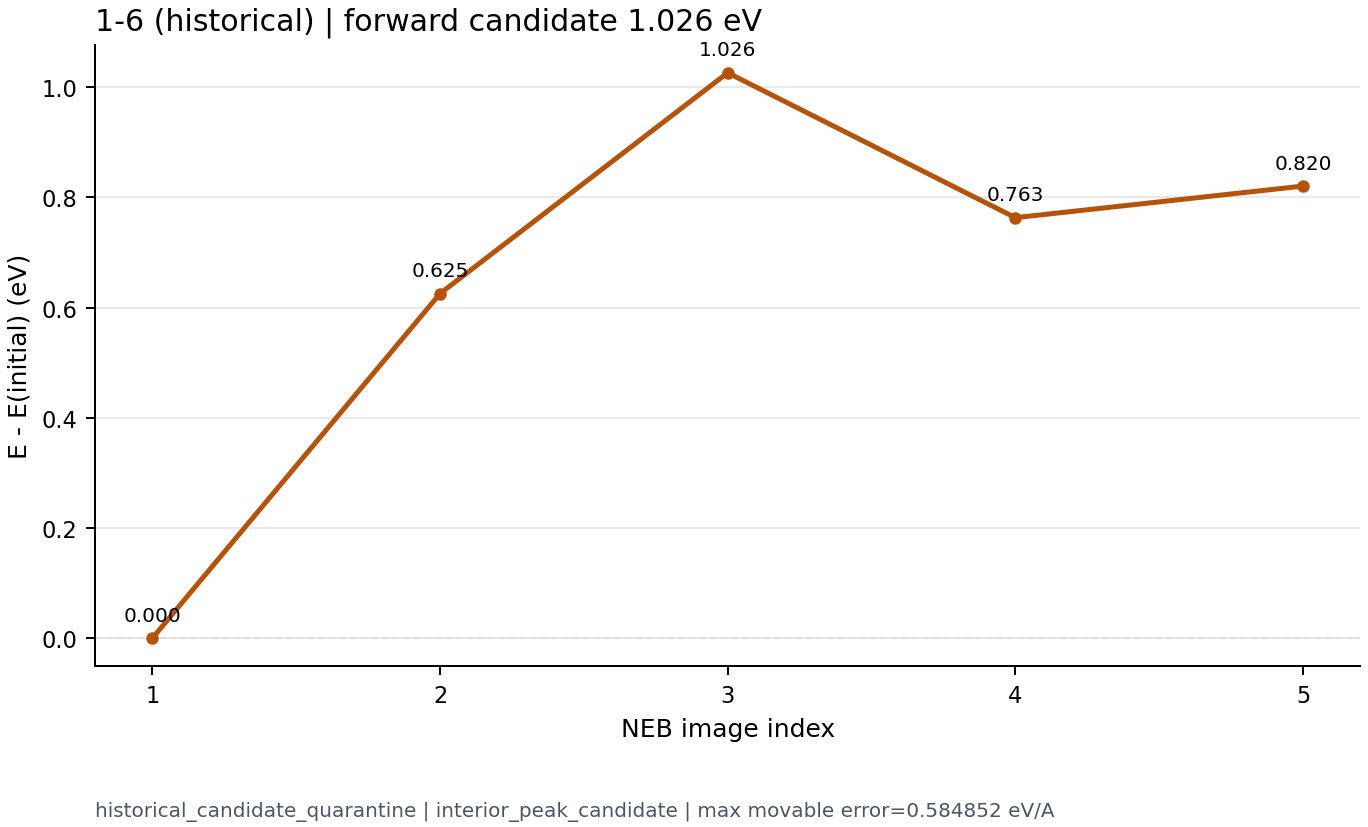
\includegraphics[width=\linewidth,height=0.42\textheight,keepaspectratio]{figure_pages/assets/fig_116.png}
\caption{Archived neb barrier inventory with convergence and provenance flags. This page shows the candidate output ``1 6 historical'' within the audited ARCHIVE-NEB-BARRIER family. The panel identity, source scope, and current status are retained in the accompanying evidence matrix.}
\label{fig:candidate_116}
\end{figure}
\textbf{Results text draft.} The bars or points retain candidate, unconverged, diverged, and accepted statuses rather than collapsing them into one ranking. Barrier values are interpreted only together with path identity and convergence metadata.
\textbf{Discussion and boundary.} Only rows that satisfy the final convergence criterion may serve as quantitative reference values. The remaining entries are useful for audit history and restart planning.
\textbf{Article placement.} Proposed article location: SI DFT NEB barrier inventory.
\textbf{Reviewer linkage:} overall status PARTIAL.
\begin{itemize}[leftmargin=1.4em,noitemsep]
\item \textbf{REV-A1 (PARTIAL):} Reconcile Fig. 3d fixed-geometry DFT-path scoring with SI Fig. S3 self-consistent MLFF-NEB, including pathway identity and the DFT reference. \emph{Completed:} The fixed-path versus self-relaxed operator distinction and the narrower model-reported-barrier wording are integrated. \emph{Still required:} Close the restartable QE path-1--4 convergence gate, preserve the final path/source metadata, and complete the SI Fig. S3 endpoint/checkpoint/optimizer/source audit before calling the quantitative reference final.
\end{itemize}
\textbf{Evidence pointers.}
\begin{itemize}[leftmargin=1.4em,noitemsep]
\item Data/processed: \begingroup\scriptsize\url{paper/data/published/neb_barrier_atlas/barrier_atlas.csv}\endgroup
\item Data/processed: \begingroup\scriptsize\url{paper/data/published/neb_barrier_atlas/barrier_atlas.json}\endgroup
\item Caption/text source: \begingroup\scriptsize\url{paper/data/published/neb_barrier_atlas/README.md}\endgroup
\end{itemize}
\statusline{\textbf{Audit gap / next action:} No co-located plotting script; treat as archived derivative until source is recovered}
\vfill
\clearpage
\section{FIG-117 --- 1 6 qe r3}
\label{figpage:fig-117}
\textbf{Group:} ARCHIVE-NEB-BARRIER\quad \textbf{Evidence chain:} partial\quad \textbf{Status:} publication
\begin{figure}[H]
\centering
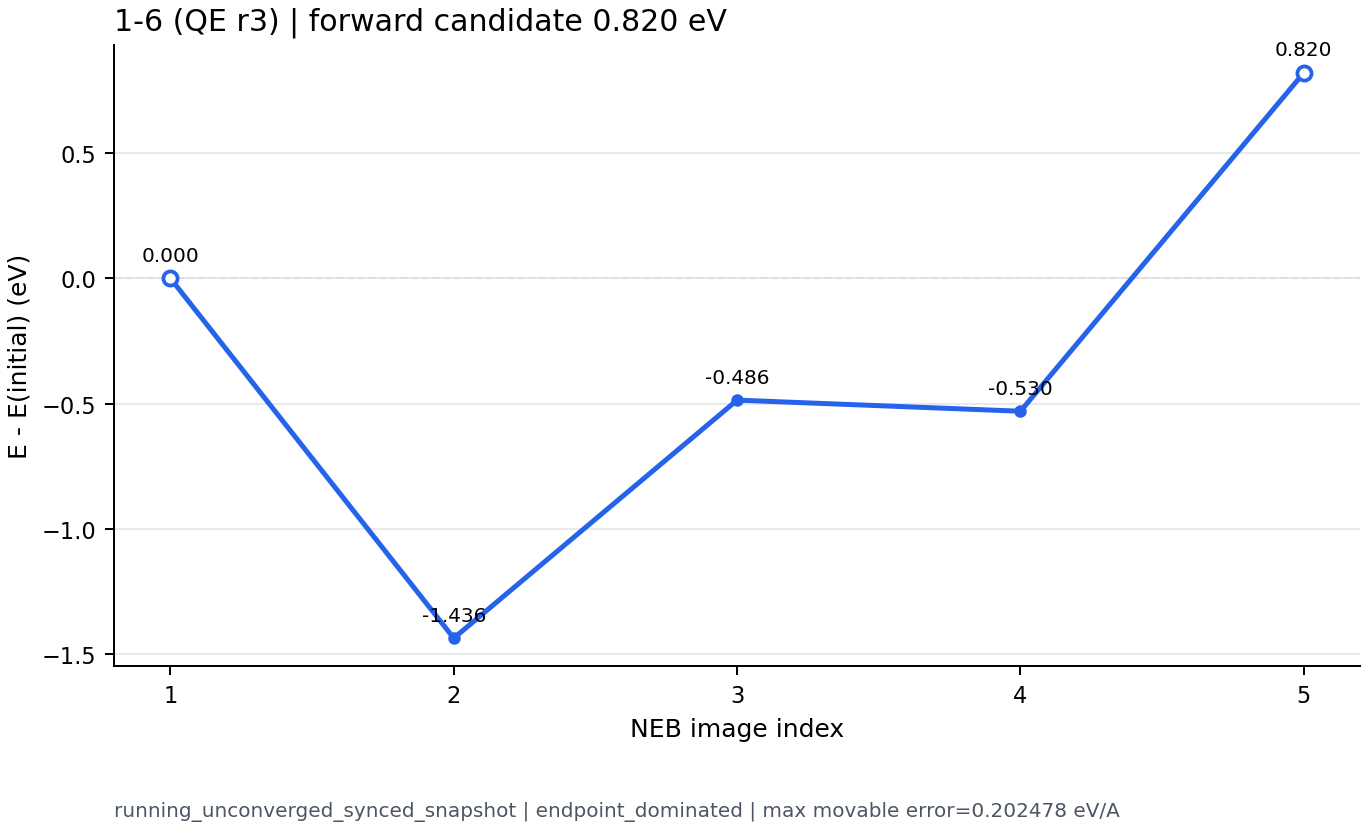
\includegraphics[width=\linewidth,height=0.42\textheight,keepaspectratio]{figure_pages/assets/fig_117.png}
\caption{Archived neb barrier inventory with convergence and provenance flags. This page shows the candidate output ``1 6 qe r3'' within the audited ARCHIVE-NEB-BARRIER family. The panel identity, source scope, and current status are retained in the accompanying evidence matrix.}
\label{fig:candidate_117}
\end{figure}
\textbf{Results text draft.} The bars or points retain candidate, unconverged, diverged, and accepted statuses rather than collapsing them into one ranking. Barrier values are interpreted only together with path identity and convergence metadata.
\textbf{Discussion and boundary.} Only rows that satisfy the final convergence criterion may serve as quantitative reference values. The remaining entries are useful for audit history and restart planning.
\textbf{Article placement.} Proposed article location: SI DFT NEB barrier inventory.
\textbf{Reviewer linkage:} overall status PARTIAL.
\begin{itemize}[leftmargin=1.4em,noitemsep]
\item \textbf{REV-A1 (PARTIAL):} Reconcile Fig. 3d fixed-geometry DFT-path scoring with SI Fig. S3 self-consistent MLFF-NEB, including pathway identity and the DFT reference. \emph{Completed:} The fixed-path versus self-relaxed operator distinction and the narrower model-reported-barrier wording are integrated. \emph{Still required:} Close the restartable QE path-1--4 convergence gate, preserve the final path/source metadata, and complete the SI Fig. S3 endpoint/checkpoint/optimizer/source audit before calling the quantitative reference final.
\end{itemize}
\textbf{Evidence pointers.}
\begin{itemize}[leftmargin=1.4em,noitemsep]
\item Data/processed: \begingroup\scriptsize\url{paper/data/published/neb_barrier_atlas/barrier_atlas.csv}\endgroup
\item Data/processed: \begingroup\scriptsize\url{paper/data/published/neb_barrier_atlas/barrier_atlas.json}\endgroup
\item Caption/text source: \begingroup\scriptsize\url{paper/data/published/neb_barrier_atlas/README.md}\endgroup
\end{itemize}
\statusline{\textbf{Audit gap / next action:} No co-located plotting script; treat as archived derivative until source is recovered}
\vfill
\clearpage
\section{FIG-118 --- 1 7 historical}
\label{figpage:fig-118}
\textbf{Group:} ARCHIVE-NEB-BARRIER\quad \textbf{Evidence chain:} partial\quad \textbf{Status:} publication;old\_or\_legacy
\begin{figure}[H]
\centering
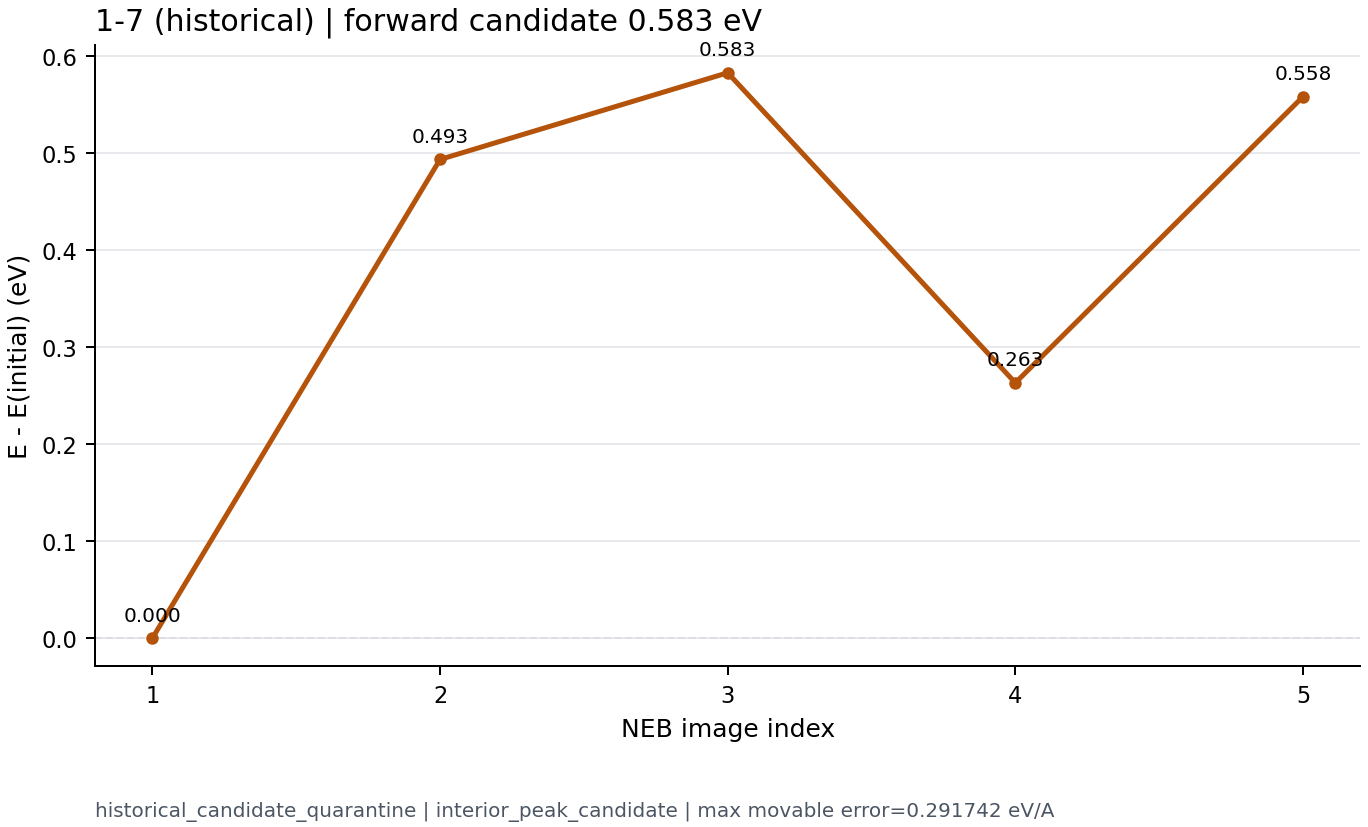
\includegraphics[width=\linewidth,height=0.42\textheight,keepaspectratio]{figure_pages/assets/fig_118.png}
\caption{Archived neb barrier inventory with convergence and provenance flags. This page shows the candidate output ``1 7 historical'' within the audited ARCHIVE-NEB-BARRIER family. The panel identity, source scope, and current status are retained in the accompanying evidence matrix.}
\label{fig:candidate_118}
\end{figure}
\textbf{Results text draft.} The bars or points retain candidate, unconverged, diverged, and accepted statuses rather than collapsing them into one ranking. Barrier values are interpreted only together with path identity and convergence metadata.
\textbf{Discussion and boundary.} Only rows that satisfy the final convergence criterion may serve as quantitative reference values. The remaining entries are useful for audit history and restart planning.
\textbf{Article placement.} Proposed article location: SI DFT NEB barrier inventory.
\textbf{Reviewer linkage:} overall status PARTIAL.
\begin{itemize}[leftmargin=1.4em,noitemsep]
\item \textbf{REV-A1 (PARTIAL):} Reconcile Fig. 3d fixed-geometry DFT-path scoring with SI Fig. S3 self-consistent MLFF-NEB, including pathway identity and the DFT reference. \emph{Completed:} The fixed-path versus self-relaxed operator distinction and the narrower model-reported-barrier wording are integrated. \emph{Still required:} Close the restartable QE path-1--4 convergence gate, preserve the final path/source metadata, and complete the SI Fig. S3 endpoint/checkpoint/optimizer/source audit before calling the quantitative reference final.
\end{itemize}
\textbf{Evidence pointers.}
\begin{itemize}[leftmargin=1.4em,noitemsep]
\item Data/processed: \begingroup\scriptsize\url{paper/data/published/neb_barrier_atlas/barrier_atlas.csv}\endgroup
\item Data/processed: \begingroup\scriptsize\url{paper/data/published/neb_barrier_atlas/barrier_atlas.json}\endgroup
\item Caption/text source: \begingroup\scriptsize\url{paper/data/published/neb_barrier_atlas/README.md}\endgroup
\end{itemize}
\statusline{\textbf{Audit gap / next action:} No co-located plotting script; treat as archived derivative until source is recovered}
\vfill
\clearpage
\section{FIG-119 --- 1 7 qe r3}
\label{figpage:fig-119}
\textbf{Group:} ARCHIVE-NEB-BARRIER\quad \textbf{Evidence chain:} partial\quad \textbf{Status:} publication
\begin{figure}[H]
\centering
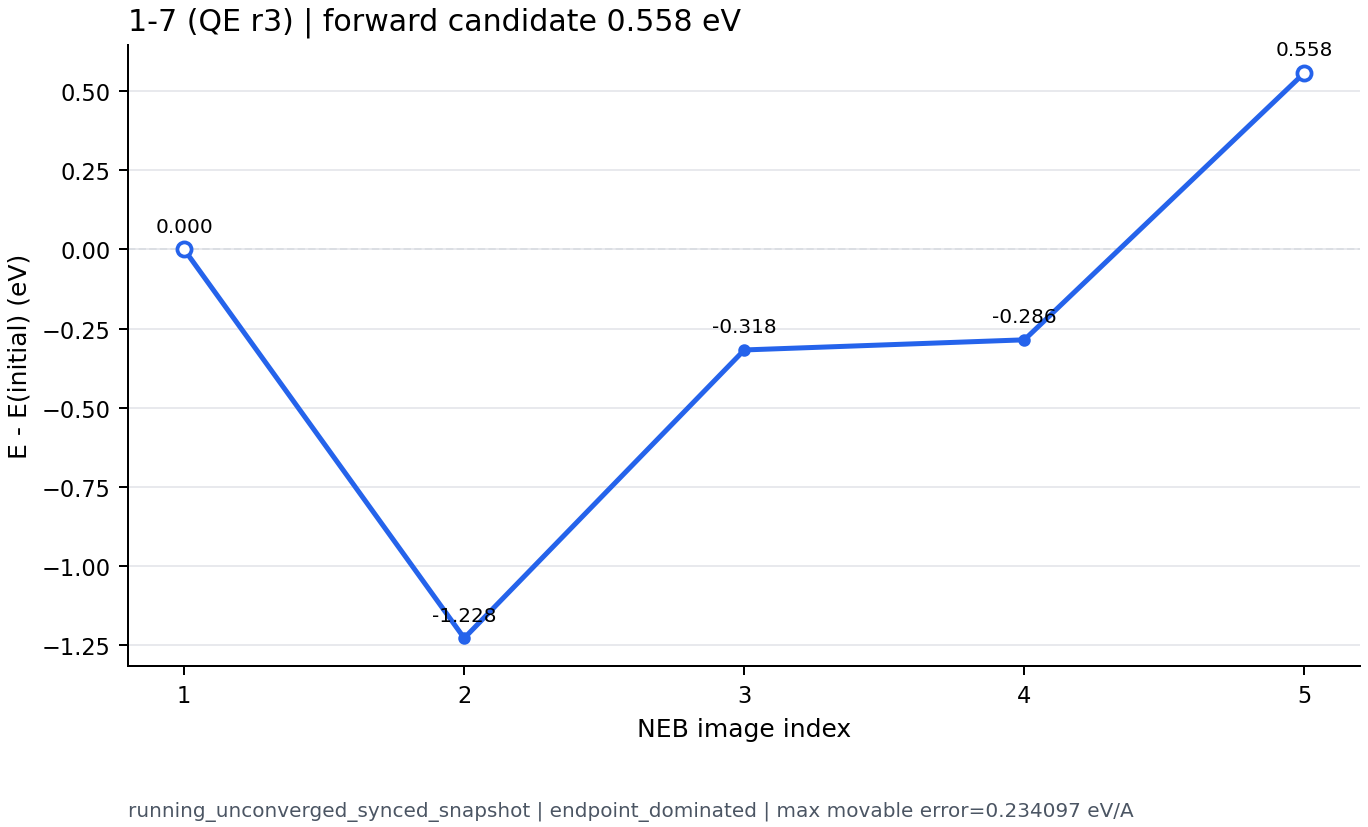
\includegraphics[width=\linewidth,height=0.42\textheight,keepaspectratio]{figure_pages/assets/fig_119.png}
\caption{Archived neb barrier inventory with convergence and provenance flags. This page shows the candidate output ``1 7 qe r3'' within the audited ARCHIVE-NEB-BARRIER family. The panel identity, source scope, and current status are retained in the accompanying evidence matrix.}
\label{fig:candidate_119}
\end{figure}
\textbf{Results text draft.} The bars or points retain candidate, unconverged, diverged, and accepted statuses rather than collapsing them into one ranking. Barrier values are interpreted only together with path identity and convergence metadata.
\textbf{Discussion and boundary.} Only rows that satisfy the final convergence criterion may serve as quantitative reference values. The remaining entries are useful for audit history and restart planning.
\textbf{Article placement.} Proposed article location: SI DFT NEB barrier inventory.
\textbf{Reviewer linkage:} overall status PARTIAL.
\begin{itemize}[leftmargin=1.4em,noitemsep]
\item \textbf{REV-A1 (PARTIAL):} Reconcile Fig. 3d fixed-geometry DFT-path scoring with SI Fig. S3 self-consistent MLFF-NEB, including pathway identity and the DFT reference. \emph{Completed:} The fixed-path versus self-relaxed operator distinction and the narrower model-reported-barrier wording are integrated. \emph{Still required:} Close the restartable QE path-1--4 convergence gate, preserve the final path/source metadata, and complete the SI Fig. S3 endpoint/checkpoint/optimizer/source audit before calling the quantitative reference final.
\end{itemize}
\textbf{Evidence pointers.}
\begin{itemize}[leftmargin=1.4em,noitemsep]
\item Data/processed: \begingroup\scriptsize\url{paper/data/published/neb_barrier_atlas/barrier_atlas.csv}\endgroup
\item Data/processed: \begingroup\scriptsize\url{paper/data/published/neb_barrier_atlas/barrier_atlas.json}\endgroup
\item Caption/text source: \begingroup\scriptsize\url{paper/data/published/neb_barrier_atlas/README.md}\endgroup
\end{itemize}
\statusline{\textbf{Audit gap / next action:} No co-located plotting script; treat as archived derivative until source is recovered}
\vfill
\clearpage
\section{FIG-120 --- 1 8 historical}
\label{figpage:fig-120}
\textbf{Group:} ARCHIVE-NEB-BARRIER\quad \textbf{Evidence chain:} partial\quad \textbf{Status:} publication;old\_or\_legacy
\begin{figure}[H]
\centering
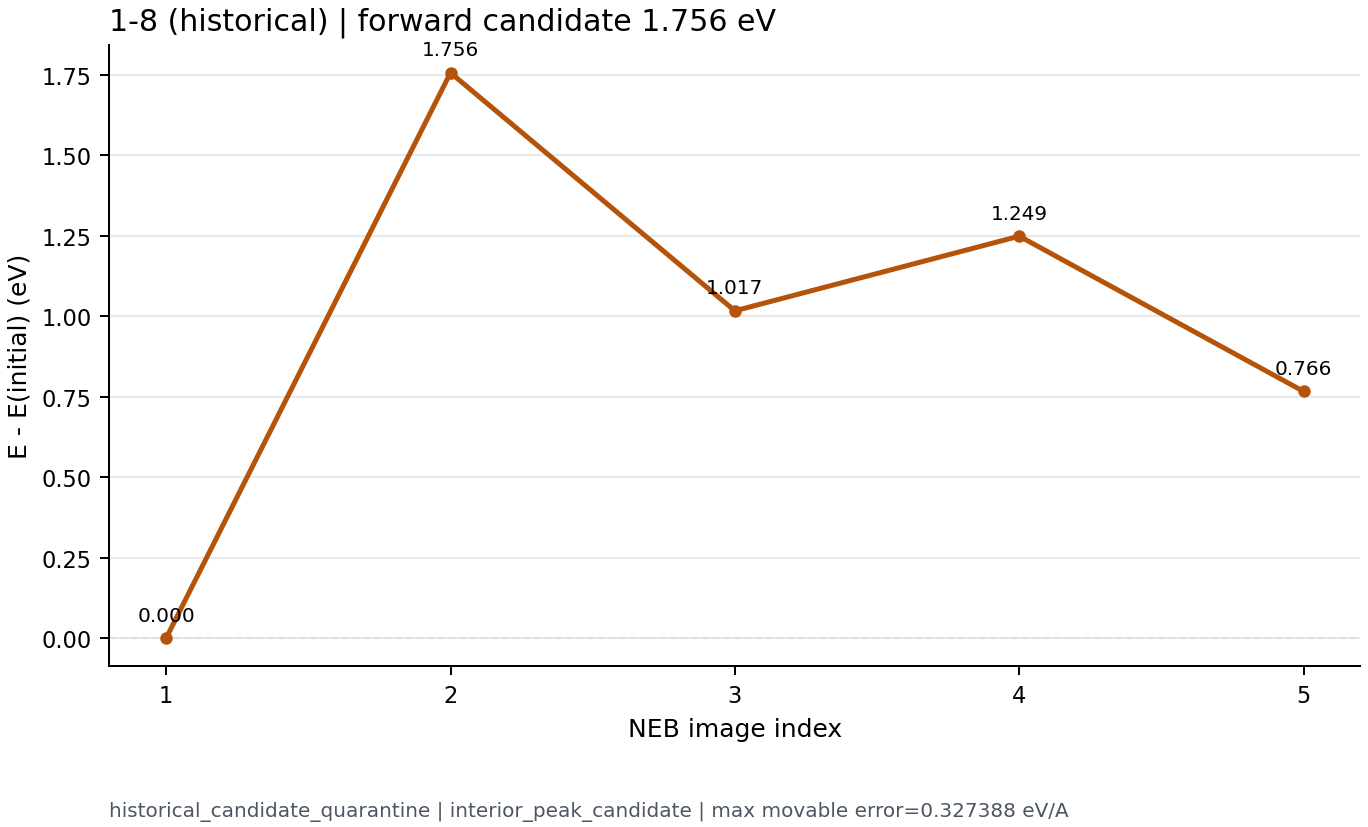
\includegraphics[width=\linewidth,height=0.42\textheight,keepaspectratio]{figure_pages/assets/fig_120.png}
\caption{Archived neb barrier inventory with convergence and provenance flags. This page shows the candidate output ``1 8 historical'' within the audited ARCHIVE-NEB-BARRIER family. The panel identity, source scope, and current status are retained in the accompanying evidence matrix.}
\label{fig:candidate_120}
\end{figure}
\textbf{Results text draft.} The bars or points retain candidate, unconverged, diverged, and accepted statuses rather than collapsing them into one ranking. Barrier values are interpreted only together with path identity and convergence metadata.
\textbf{Discussion and boundary.} Only rows that satisfy the final convergence criterion may serve as quantitative reference values. The remaining entries are useful for audit history and restart planning.
\textbf{Article placement.} Proposed article location: SI DFT NEB barrier inventory.
\textbf{Reviewer linkage:} overall status PARTIAL.
\begin{itemize}[leftmargin=1.4em,noitemsep]
\item \textbf{REV-A1 (PARTIAL):} Reconcile Fig. 3d fixed-geometry DFT-path scoring with SI Fig. S3 self-consistent MLFF-NEB, including pathway identity and the DFT reference. \emph{Completed:} The fixed-path versus self-relaxed operator distinction and the narrower model-reported-barrier wording are integrated. \emph{Still required:} Close the restartable QE path-1--4 convergence gate, preserve the final path/source metadata, and complete the SI Fig. S3 endpoint/checkpoint/optimizer/source audit before calling the quantitative reference final.
\end{itemize}
\textbf{Evidence pointers.}
\begin{itemize}[leftmargin=1.4em,noitemsep]
\item Data/processed: \begingroup\scriptsize\url{paper/data/published/neb_barrier_atlas/barrier_atlas.csv}\endgroup
\item Data/processed: \begingroup\scriptsize\url{paper/data/published/neb_barrier_atlas/barrier_atlas.json}\endgroup
\item Caption/text source: \begingroup\scriptsize\url{paper/data/published/neb_barrier_atlas/README.md}\endgroup
\end{itemize}
\statusline{\textbf{Audit gap / next action:} No co-located plotting script; treat as archived derivative until source is recovered}
\vfill
\clearpage
\section{FIG-121 --- 81 neb 1}
\label{figpage:fig-121}
\textbf{Group:} ARCHIVE-NEB-BARRIER\quad \textbf{Evidence chain:} partial\quad \textbf{Status:} publication
\begin{figure}[H]
\centering
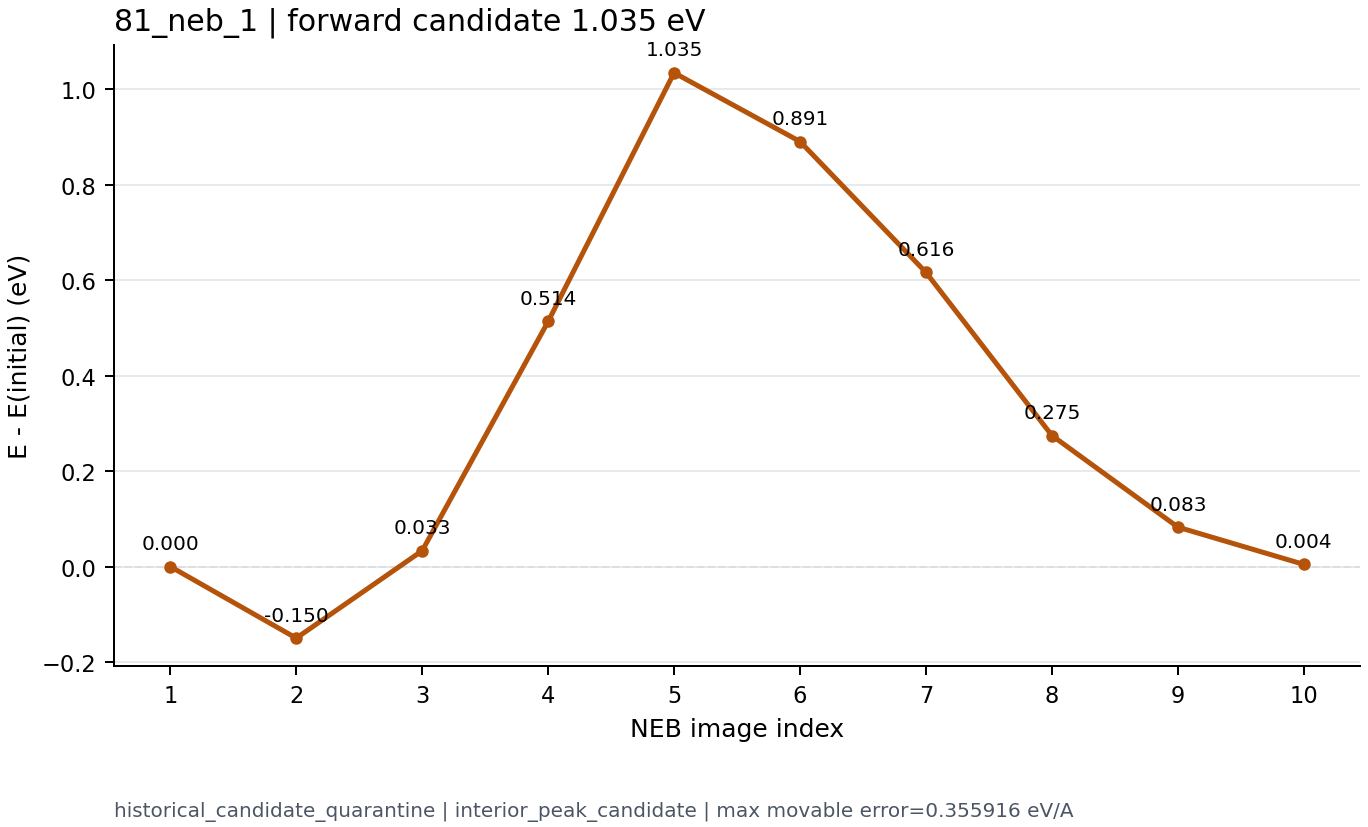
\includegraphics[width=\linewidth,height=0.42\textheight,keepaspectratio]{figure_pages/assets/fig_121.png}
\caption{Archived neb barrier inventory with convergence and provenance flags. This page shows the candidate output ``81 neb 1'' within the audited ARCHIVE-NEB-BARRIER family. The panel identity, source scope, and current status are retained in the accompanying evidence matrix.}
\label{fig:candidate_121}
\end{figure}
\textbf{Results text draft.} The bars or points retain candidate, unconverged, diverged, and accepted statuses rather than collapsing them into one ranking. Barrier values are interpreted only together with path identity and convergence metadata.
\textbf{Discussion and boundary.} Only rows that satisfy the final convergence criterion may serve as quantitative reference values. The remaining entries are useful for audit history and restart planning.
\textbf{Article placement.} Proposed article location: SI DFT NEB barrier inventory.
\textbf{Reviewer linkage:} overall status PARTIAL.
\begin{itemize}[leftmargin=1.4em,noitemsep]
\item \textbf{REV-A1 (PARTIAL):} Reconcile Fig. 3d fixed-geometry DFT-path scoring with SI Fig. S3 self-consistent MLFF-NEB, including pathway identity and the DFT reference. \emph{Completed:} The fixed-path versus self-relaxed operator distinction and the narrower model-reported-barrier wording are integrated. \emph{Still required:} Close the restartable QE path-1--4 convergence gate, preserve the final path/source metadata, and complete the SI Fig. S3 endpoint/checkpoint/optimizer/source audit before calling the quantitative reference final.
\end{itemize}
\textbf{Evidence pointers.}
\begin{itemize}[leftmargin=1.4em,noitemsep]
\item Data/processed: \begingroup\scriptsize\url{paper/data/published/neb_barrier_atlas/barrier_atlas.csv}\endgroup
\item Data/processed: \begingroup\scriptsize\url{paper/data/published/neb_barrier_atlas/barrier_atlas.json}\endgroup
\item Caption/text source: \begingroup\scriptsize\url{paper/data/published/neb_barrier_atlas/README.md}\endgroup
\end{itemize}
\statusline{\textbf{Audit gap / next action:} No co-located plotting script; treat as archived derivative until source is recovered}
\vfill
\clearpage
\section{FIG-122 --- 81 neb 2}
\label{figpage:fig-122}
\textbf{Group:} ARCHIVE-NEB-BARRIER\quad \textbf{Evidence chain:} partial\quad \textbf{Status:} publication
\begin{figure}[H]
\centering
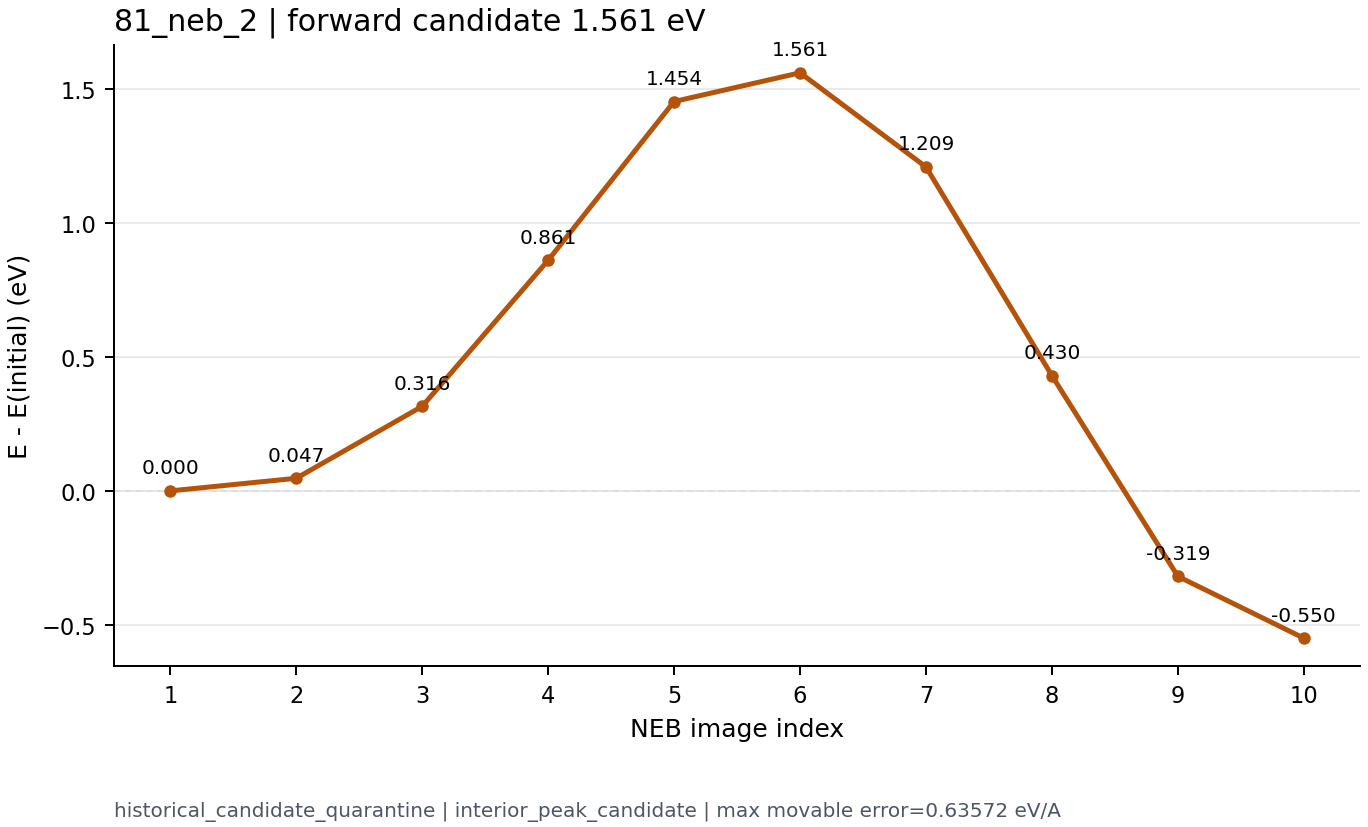
\includegraphics[width=\linewidth,height=0.42\textheight,keepaspectratio]{figure_pages/assets/fig_122.png}
\caption{Archived neb barrier inventory with convergence and provenance flags. This page shows the candidate output ``81 neb 2'' within the audited ARCHIVE-NEB-BARRIER family. The panel identity, source scope, and current status are retained in the accompanying evidence matrix.}
\label{fig:candidate_122}
\end{figure}
\textbf{Results text draft.} The bars or points retain candidate, unconverged, diverged, and accepted statuses rather than collapsing them into one ranking. Barrier values are interpreted only together with path identity and convergence metadata.
\textbf{Discussion and boundary.} Only rows that satisfy the final convergence criterion may serve as quantitative reference values. The remaining entries are useful for audit history and restart planning.
\textbf{Article placement.} Proposed article location: SI DFT NEB barrier inventory.
\textbf{Reviewer linkage:} overall status PARTIAL.
\begin{itemize}[leftmargin=1.4em,noitemsep]
\item \textbf{REV-A1 (PARTIAL):} Reconcile Fig. 3d fixed-geometry DFT-path scoring with SI Fig. S3 self-consistent MLFF-NEB, including pathway identity and the DFT reference. \emph{Completed:} The fixed-path versus self-relaxed operator distinction and the narrower model-reported-barrier wording are integrated. \emph{Still required:} Close the restartable QE path-1--4 convergence gate, preserve the final path/source metadata, and complete the SI Fig. S3 endpoint/checkpoint/optimizer/source audit before calling the quantitative reference final.
\end{itemize}
\textbf{Evidence pointers.}
\begin{itemize}[leftmargin=1.4em,noitemsep]
\item Data/processed: \begingroup\scriptsize\url{paper/data/published/neb_barrier_atlas/barrier_atlas.csv}\endgroup
\item Data/processed: \begingroup\scriptsize\url{paper/data/published/neb_barrier_atlas/barrier_atlas.json}\endgroup
\item Caption/text source: \begingroup\scriptsize\url{paper/data/published/neb_barrier_atlas/README.md}\endgroup
\end{itemize}
\statusline{\textbf{Audit gap / next action:} No co-located plotting script; treat as archived derivative until source is recovered}
\vfill
\clearpage
\section{FIG-123 --- 81 neb 3}
\label{figpage:fig-123}
\textbf{Group:} ARCHIVE-NEB-BARRIER\quad \textbf{Evidence chain:} partial\quad \textbf{Status:} publication
\begin{figure}[H]
\centering
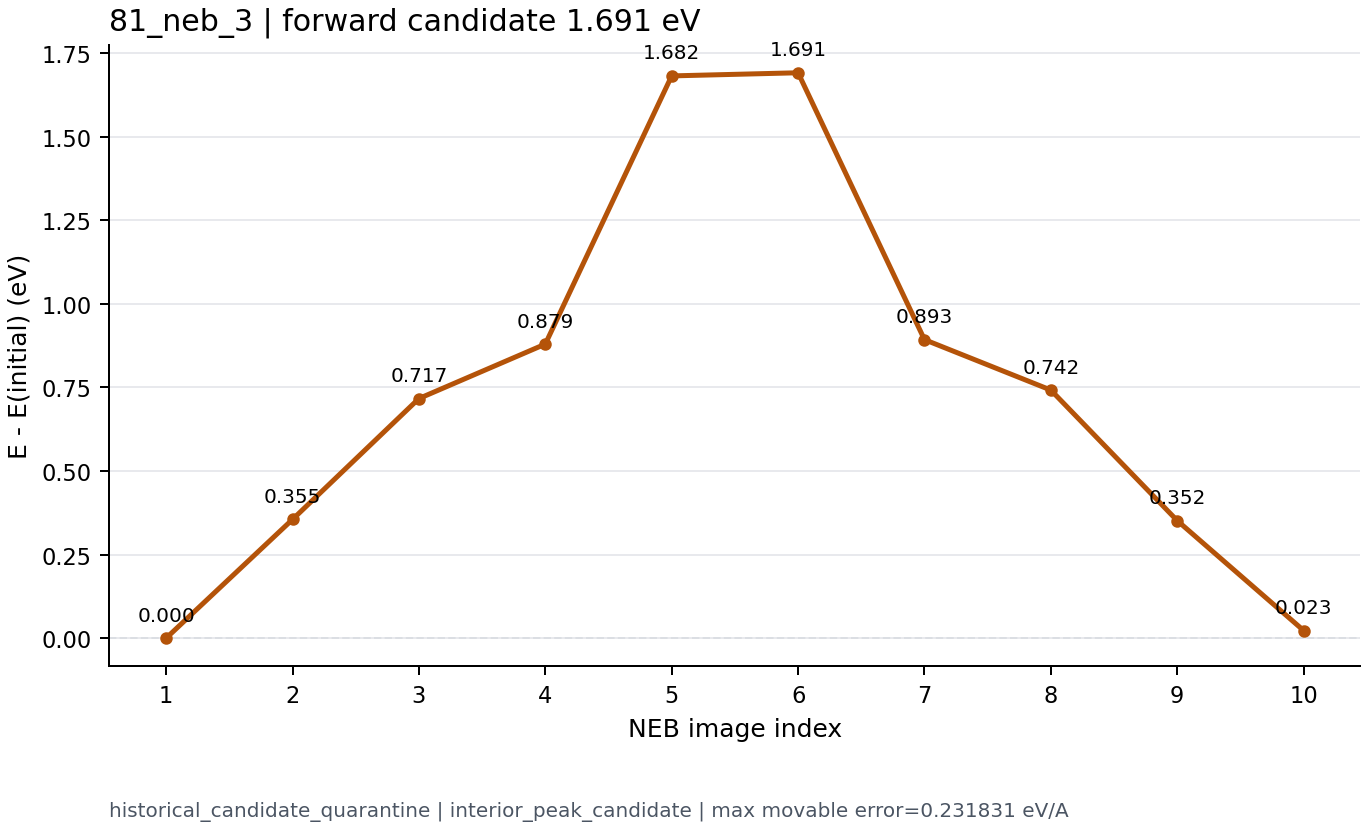
\includegraphics[width=\linewidth,height=0.42\textheight,keepaspectratio]{figure_pages/assets/fig_123.png}
\caption{Archived neb barrier inventory with convergence and provenance flags. This page shows the candidate output ``81 neb 3'' within the audited ARCHIVE-NEB-BARRIER family. The panel identity, source scope, and current status are retained in the accompanying evidence matrix.}
\label{fig:candidate_123}
\end{figure}
\textbf{Results text draft.} The bars or points retain candidate, unconverged, diverged, and accepted statuses rather than collapsing them into one ranking. Barrier values are interpreted only together with path identity and convergence metadata.
\textbf{Discussion and boundary.} Only rows that satisfy the final convergence criterion may serve as quantitative reference values. The remaining entries are useful for audit history and restart planning.
\textbf{Article placement.} Proposed article location: SI DFT NEB barrier inventory.
\textbf{Reviewer linkage:} overall status PARTIAL.
\begin{itemize}[leftmargin=1.4em,noitemsep]
\item \textbf{REV-A1 (PARTIAL):} Reconcile Fig. 3d fixed-geometry DFT-path scoring with SI Fig. S3 self-consistent MLFF-NEB, including pathway identity and the DFT reference. \emph{Completed:} The fixed-path versus self-relaxed operator distinction and the narrower model-reported-barrier wording are integrated. \emph{Still required:} Close the restartable QE path-1--4 convergence gate, preserve the final path/source metadata, and complete the SI Fig. S3 endpoint/checkpoint/optimizer/source audit before calling the quantitative reference final.
\end{itemize}
\textbf{Evidence pointers.}
\begin{itemize}[leftmargin=1.4em,noitemsep]
\item Data/processed: \begingroup\scriptsize\url{paper/data/published/neb_barrier_atlas/barrier_atlas.csv}\endgroup
\item Data/processed: \begingroup\scriptsize\url{paper/data/published/neb_barrier_atlas/barrier_atlas.json}\endgroup
\item Caption/text source: \begingroup\scriptsize\url{paper/data/published/neb_barrier_atlas/README.md}\endgroup
\end{itemize}
\statusline{\textbf{Audit gap / next action:} No co-located plotting script; treat as archived derivative until source is recovered}
\vfill
\clearpage
\section{FIG-124 --- 81 neb 4}
\label{figpage:fig-124}
\textbf{Group:} ARCHIVE-NEB-BARRIER\quad \textbf{Evidence chain:} partial\quad \textbf{Status:} publication
\begin{figure}[H]
\centering
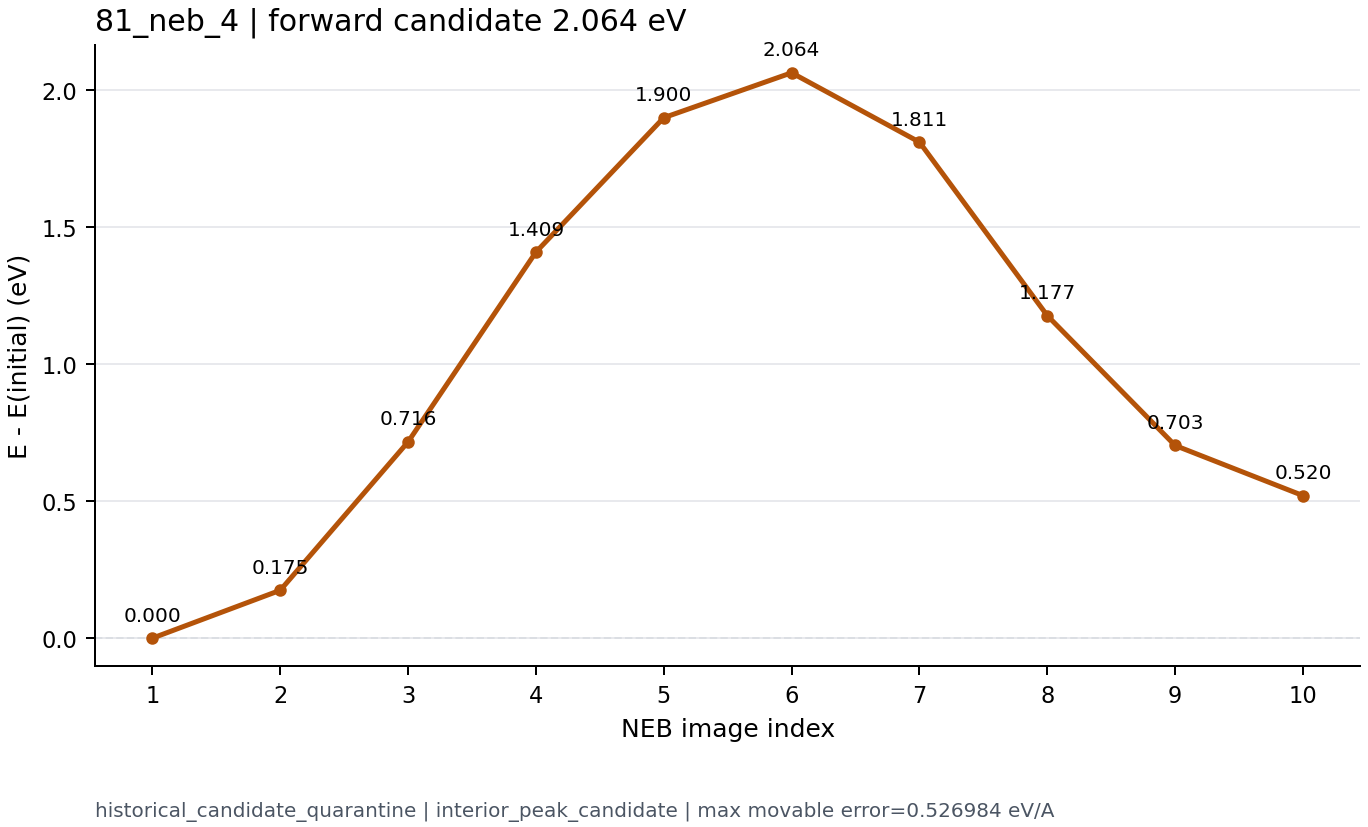
\includegraphics[width=\linewidth,height=0.42\textheight,keepaspectratio]{figure_pages/assets/fig_124.png}
\caption{Archived neb barrier inventory with convergence and provenance flags. This page shows the candidate output ``81 neb 4'' within the audited ARCHIVE-NEB-BARRIER family. The panel identity, source scope, and current status are retained in the accompanying evidence matrix.}
\label{fig:candidate_124}
\end{figure}
\textbf{Results text draft.} The bars or points retain candidate, unconverged, diverged, and accepted statuses rather than collapsing them into one ranking. Barrier values are interpreted only together with path identity and convergence metadata.
\textbf{Discussion and boundary.} Only rows that satisfy the final convergence criterion may serve as quantitative reference values. The remaining entries are useful for audit history and restart planning.
\textbf{Article placement.} Proposed article location: SI DFT NEB barrier inventory.
\textbf{Reviewer linkage:} overall status PARTIAL.
\begin{itemize}[leftmargin=1.4em,noitemsep]
\item \textbf{REV-A1 (PARTIAL):} Reconcile Fig. 3d fixed-geometry DFT-path scoring with SI Fig. S3 self-consistent MLFF-NEB, including pathway identity and the DFT reference. \emph{Completed:} The fixed-path versus self-relaxed operator distinction and the narrower model-reported-barrier wording are integrated. \emph{Still required:} Close the restartable QE path-1--4 convergence gate, preserve the final path/source metadata, and complete the SI Fig. S3 endpoint/checkpoint/optimizer/source audit before calling the quantitative reference final.
\end{itemize}
\textbf{Evidence pointers.}
\begin{itemize}[leftmargin=1.4em,noitemsep]
\item Data/processed: \begingroup\scriptsize\url{paper/data/published/neb_barrier_atlas/barrier_atlas.csv}\endgroup
\item Data/processed: \begingroup\scriptsize\url{paper/data/published/neb_barrier_atlas/barrier_atlas.json}\endgroup
\item Caption/text source: \begingroup\scriptsize\url{paper/data/published/neb_barrier_atlas/README.md}\endgroup
\end{itemize}
\statusline{\textbf{Audit gap / next action:} No co-located plotting script; treat as archived derivative until source is recovered}
\vfill
\clearpage
\section{FIG-125 --- 81 neb 5}
\label{figpage:fig-125}
\textbf{Group:} ARCHIVE-NEB-BARRIER\quad \textbf{Evidence chain:} partial\quad \textbf{Status:} publication
\begin{figure}[H]
\centering
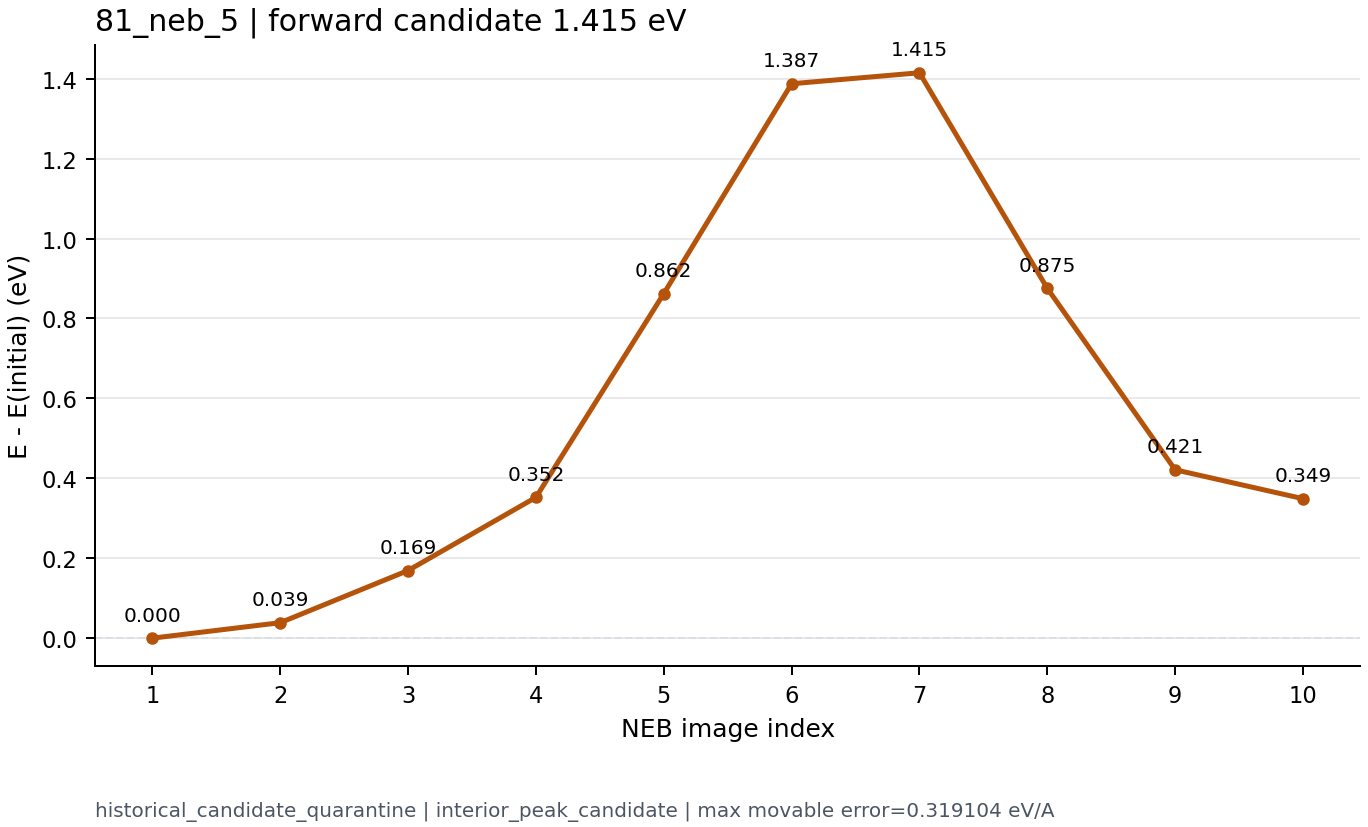
\includegraphics[width=\linewidth,height=0.42\textheight,keepaspectratio]{figure_pages/assets/fig_125.png}
\caption{Archived neb barrier inventory with convergence and provenance flags. This page shows the candidate output ``81 neb 5'' within the audited ARCHIVE-NEB-BARRIER family. The panel identity, source scope, and current status are retained in the accompanying evidence matrix.}
\label{fig:candidate_125}
\end{figure}
\textbf{Results text draft.} The bars or points retain candidate, unconverged, diverged, and accepted statuses rather than collapsing them into one ranking. Barrier values are interpreted only together with path identity and convergence metadata.
\textbf{Discussion and boundary.} Only rows that satisfy the final convergence criterion may serve as quantitative reference values. The remaining entries are useful for audit history and restart planning.
\textbf{Article placement.} Proposed article location: SI DFT NEB barrier inventory.
\textbf{Reviewer linkage:} overall status PARTIAL.
\begin{itemize}[leftmargin=1.4em,noitemsep]
\item \textbf{REV-A1 (PARTIAL):} Reconcile Fig. 3d fixed-geometry DFT-path scoring with SI Fig. S3 self-consistent MLFF-NEB, including pathway identity and the DFT reference. \emph{Completed:} The fixed-path versus self-relaxed operator distinction and the narrower model-reported-barrier wording are integrated. \emph{Still required:} Close the restartable QE path-1--4 convergence gate, preserve the final path/source metadata, and complete the SI Fig. S3 endpoint/checkpoint/optimizer/source audit before calling the quantitative reference final.
\end{itemize}
\textbf{Evidence pointers.}
\begin{itemize}[leftmargin=1.4em,noitemsep]
\item Data/processed: \begingroup\scriptsize\url{paper/data/published/neb_barrier_atlas/barrier_atlas.csv}\endgroup
\item Data/processed: \begingroup\scriptsize\url{paper/data/published/neb_barrier_atlas/barrier_atlas.json}\endgroup
\item Caption/text source: \begingroup\scriptsize\url{paper/data/published/neb_barrier_atlas/README.md}\endgroup
\end{itemize}
\statusline{\textbf{Audit gap / next action:} No co-located plotting script; treat as archived derivative until source is recovered}
\vfill
\clearpage
\section{FIG-126 --- All qe neb profiles}
\label{figpage:fig-126}
\textbf{Group:} ARCHIVE-NEB-BARRIER\quad \textbf{Evidence chain:} partial\quad \textbf{Status:} publication;comparison
\begin{figure}[H]
\centering
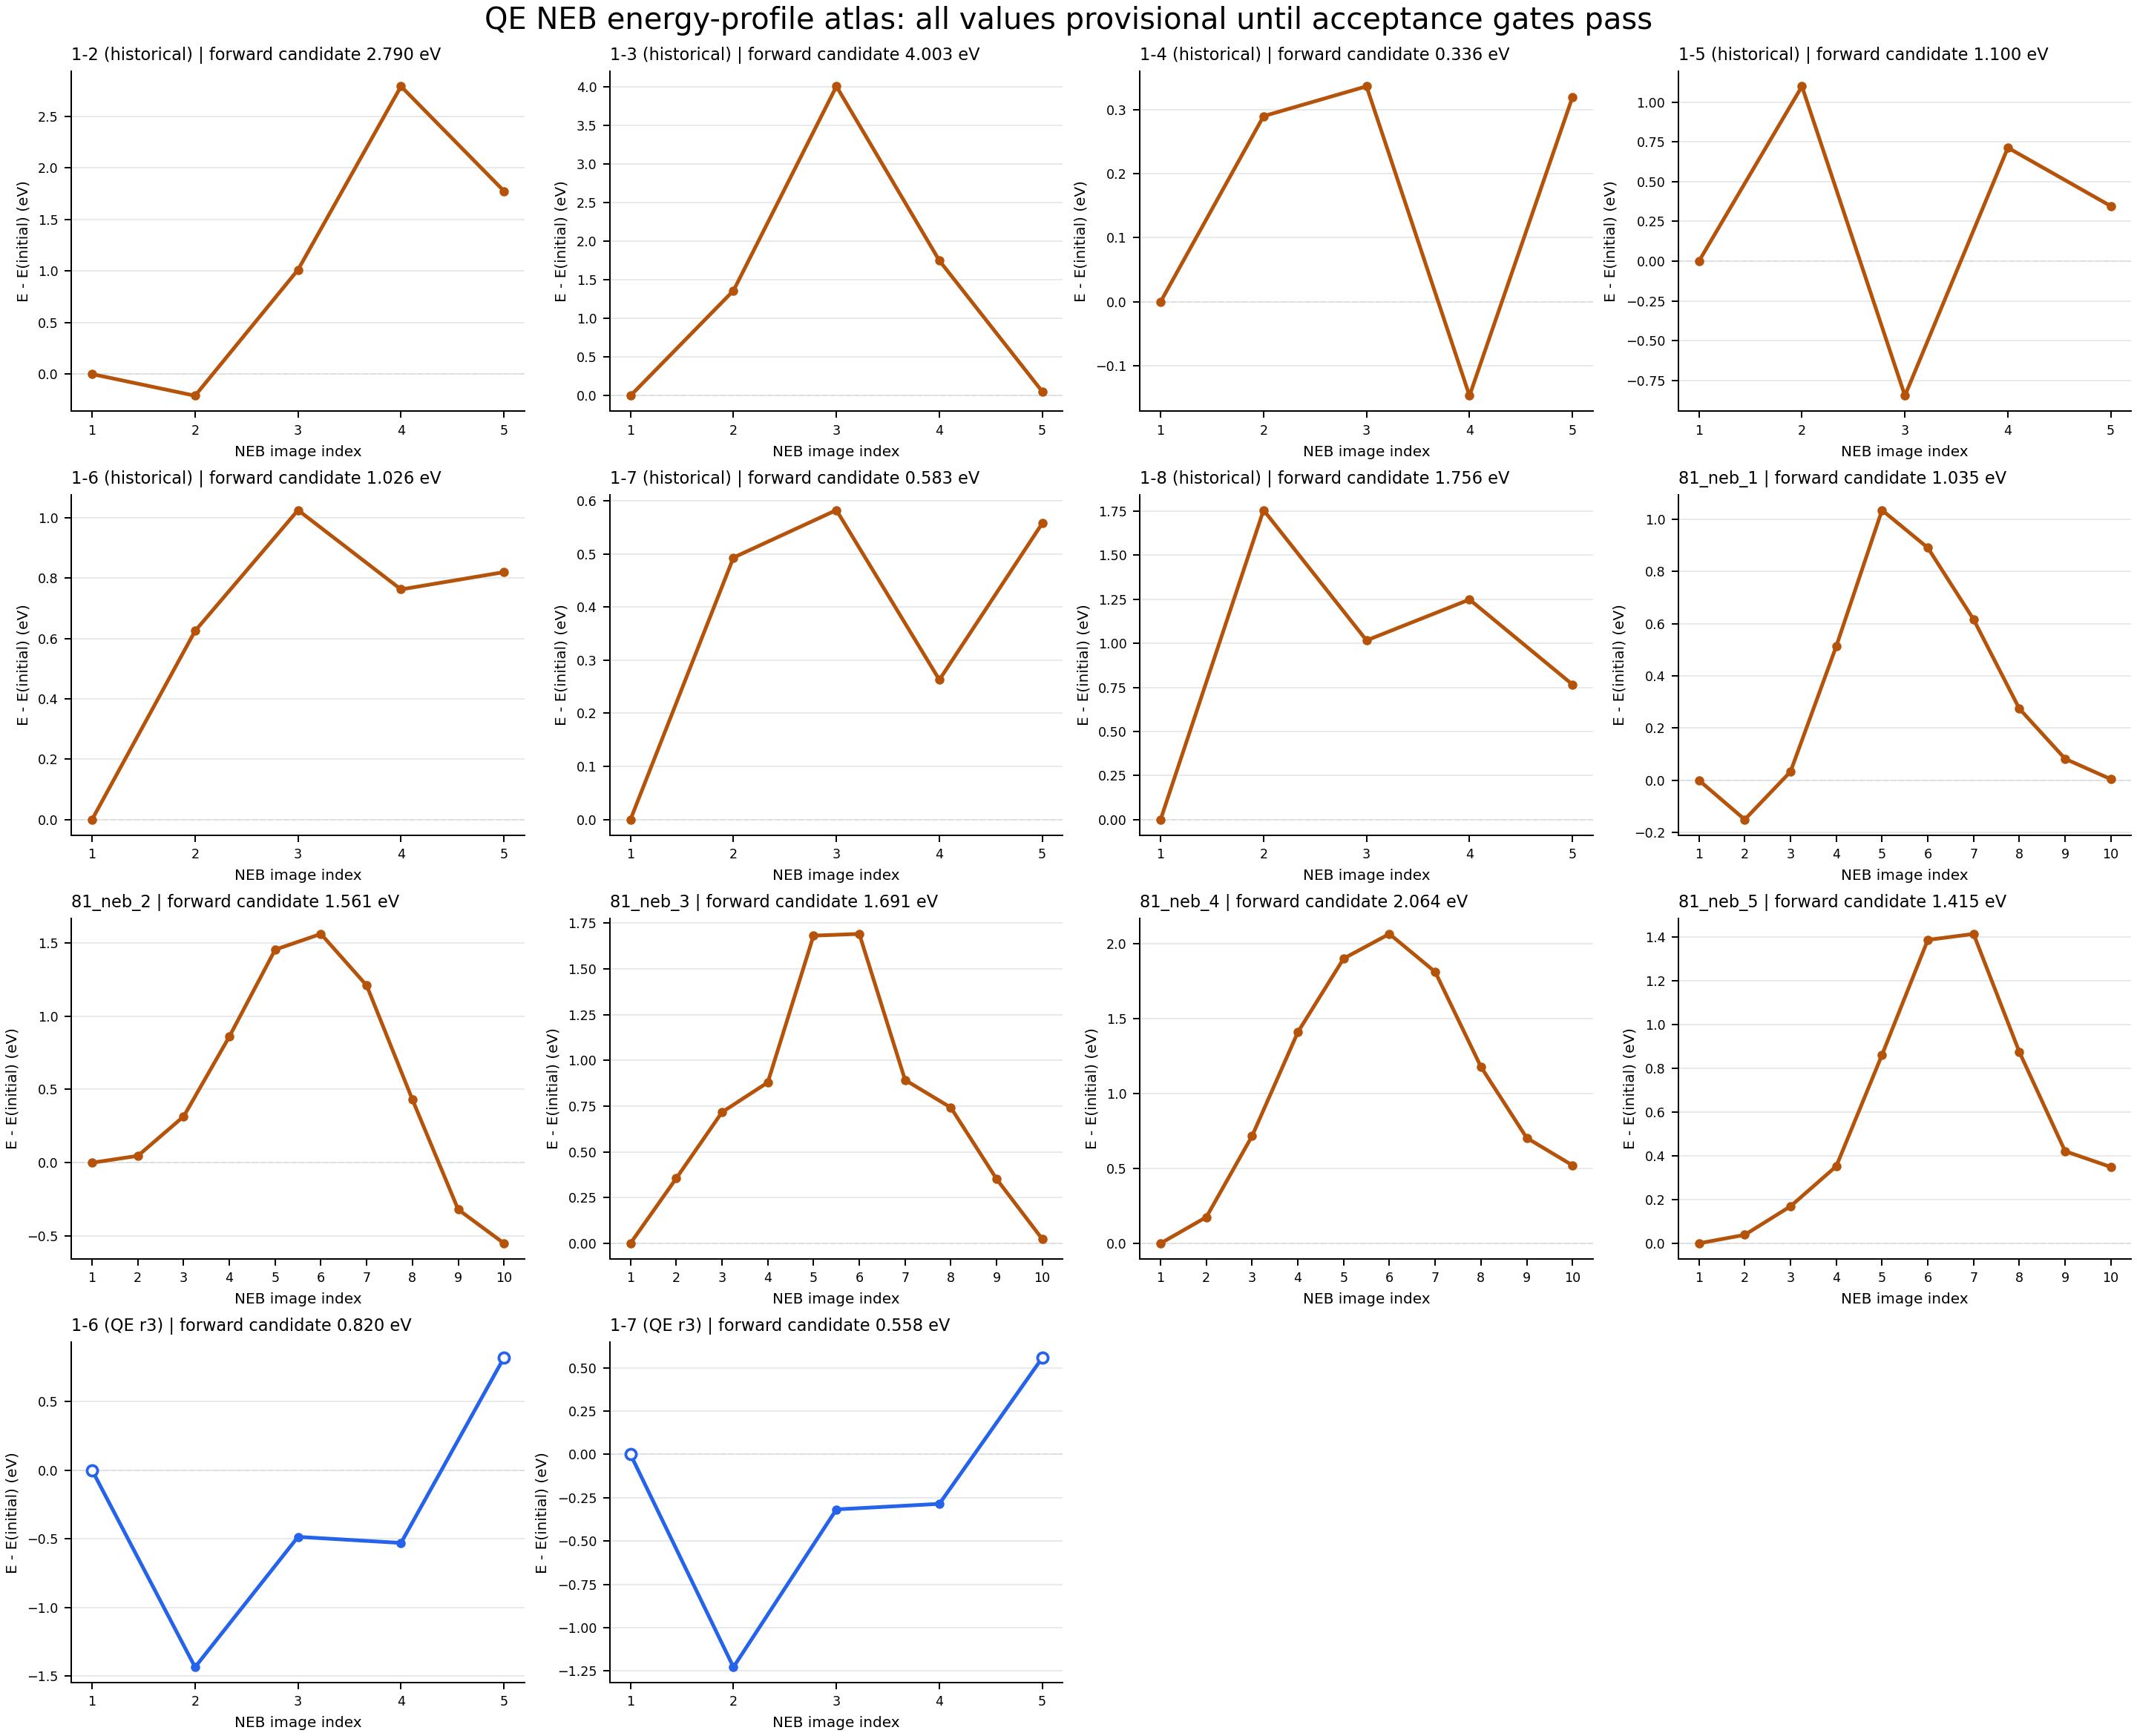
\includegraphics[width=\linewidth,height=0.42\textheight,keepaspectratio]{figure_pages/assets/fig_126.png}
\caption{Archived neb barrier inventory with convergence and provenance flags. This page shows the candidate output ``All qe neb profiles'' within the audited ARCHIVE-NEB-BARRIER family. The panel identity, source scope, and current status are retained in the accompanying evidence matrix.}
\label{fig:candidate_126}
\end{figure}
\textbf{Results text draft.} The bars or points retain candidate, unconverged, diverged, and accepted statuses rather than collapsing them into one ranking. Barrier values are interpreted only together with path identity and convergence metadata.
\textbf{Discussion and boundary.} Only rows that satisfy the final convergence criterion may serve as quantitative reference values. The remaining entries are useful for audit history and restart planning.
\textbf{Article placement.} Proposed article location: SI DFT NEB barrier inventory.
\textbf{Reviewer linkage:} overall status PARTIAL.
\begin{itemize}[leftmargin=1.4em,noitemsep]
\item \textbf{REV-A1 (PARTIAL):} Reconcile Fig. 3d fixed-geometry DFT-path scoring with SI Fig. S3 self-consistent MLFF-NEB, including pathway identity and the DFT reference. \emph{Completed:} The fixed-path versus self-relaxed operator distinction and the narrower model-reported-barrier wording are integrated. \emph{Still required:} Close the restartable QE path-1--4 convergence gate, preserve the final path/source metadata, and complete the SI Fig. S3 endpoint/checkpoint/optimizer/source audit before calling the quantitative reference final.
\end{itemize}
\textbf{Evidence pointers.}
\begin{itemize}[leftmargin=1.4em,noitemsep]
\item Data/processed: \begingroup\scriptsize\url{paper/data/published/neb_barrier_atlas/barrier_atlas.csv}\endgroup
\item Data/processed: \begingroup\scriptsize\url{paper/data/published/neb_barrier_atlas/barrier_atlas.json}\endgroup
\item Caption/text source: \begingroup\scriptsize\url{paper/data/published/neb_barrier_atlas/README.md}\endgroup
\end{itemize}
\statusline{\textbf{Audit gap / next action:} No co-located plotting script; treat as archived derivative until source is recovered}
\vfill
\clearpage
\section{FIG-127 --- 00 1 2 mb mlff cpu 1 2 s42 30791344}
\label{figpage:fig-127}
\textbf{Group:} ARCHIVE-NEB-PROFILE\quad \textbf{Evidence chain:} partial\quad \textbf{Status:} publication;comparison
\begin{figure}[H]
\centering
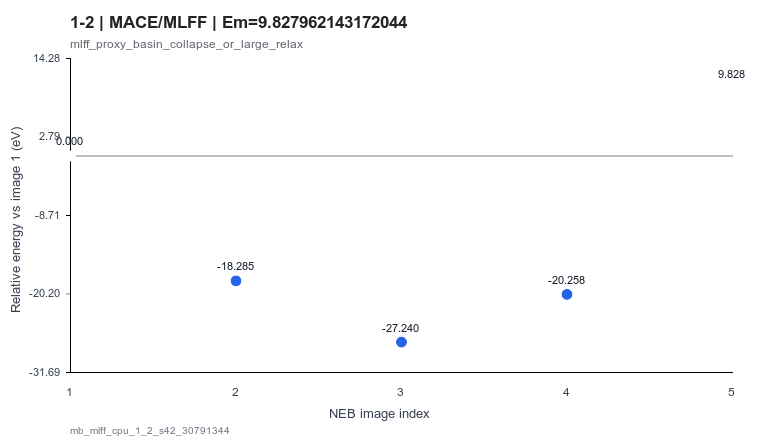
\includegraphics[width=\linewidth,height=0.42\textheight,keepaspectratio]{figure_pages/assets/fig_127.png}
\caption{Archived neb energy-profile or minimum-energy-path comparison. This page shows the candidate output ``00 1 2 mb mlff cpu 1 2 s42 30791344'' within the audited ARCHIVE-NEB-PROFILE family. The panel identity, source scope, and current status are retained in the accompanying evidence matrix.}
\label{fig:candidate_127}
\end{figure}
\textbf{Results text draft.} The profiles display the parsed path-level energy variation while preserving the distinction between reference candidates and formally converged paths. The plotted path identity is part of the evidence package.
\textbf{Discussion and boundary.} The figure supports qualitative path comparison and auditability. It must not imply final barrier accuracy for profiles that remain flagged as provisional or incomplete.
\textbf{Article placement.} Proposed article location: SI DFT NEB profiles / fixed-path benchmark.
\textbf{Reviewer linkage:} overall status PARTIAL.
\begin{itemize}[leftmargin=1.4em,noitemsep]
\item \textbf{REV-A1 (PARTIAL):} Reconcile Fig. 3d fixed-geometry DFT-path scoring with SI Fig. S3 self-consistent MLFF-NEB, including pathway identity and the DFT reference. \emph{Completed:} The fixed-path versus self-relaxed operator distinction and the narrower model-reported-barrier wording are integrated. \emph{Still required:} Close the restartable QE path-1--4 convergence gate, preserve the final path/source metadata, and complete the SI Fig. S3 endpoint/checkpoint/optimizer/source audit before calling the quantitative reference final.
\end{itemize}
\textbf{Evidence pointers.}
\begin{itemize}[leftmargin=1.4em,noitemsep]
\item Data/processed: \begingroup\scriptsize\url{paper/data/published/neb_energy_profiles/neb_energy_summary.csv}\endgroup
\item Data/processed: \begingroup\scriptsize\url{paper/data/published/neb_energy_profiles/neb_energy_summary.json}\endgroup
\item Caption/text source: \begingroup\scriptsize\url{paper/data/published/neb_energy_profiles/neb_energy_snapshot.md}\endgroup
\end{itemize}
\statusline{\textbf{Audit gap / next action:} No co-located plotting script; path-table provenance is present}
\vfill
\clearpage
\section{FIG-128 --- 02 1 3 mb mlff cpu 1 3 s42 30791345}
\label{figpage:fig-128}
\textbf{Group:} ARCHIVE-NEB-PROFILE\quad \textbf{Evidence chain:} partial\quad \textbf{Status:} publication;comparison
\begin{figure}[H]
\centering
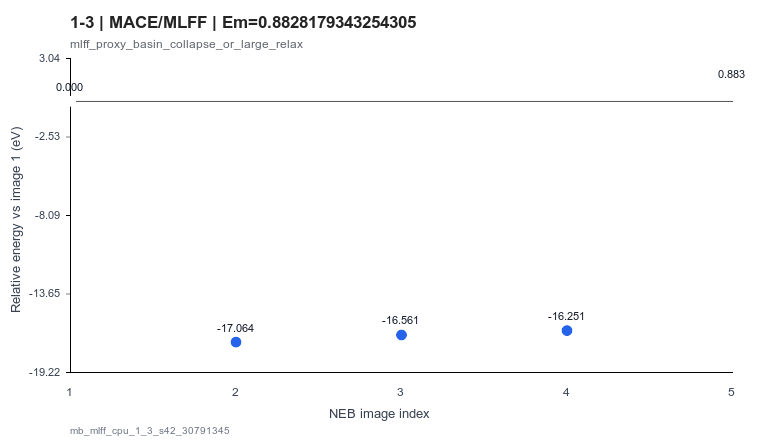
\includegraphics[width=\linewidth,height=0.42\textheight,keepaspectratio]{figure_pages/assets/fig_128.png}
\caption{Archived neb energy-profile or minimum-energy-path comparison. This page shows the candidate output ``02 1 3 mb mlff cpu 1 3 s42 30791345'' within the audited ARCHIVE-NEB-PROFILE family. The panel identity, source scope, and current status are retained in the accompanying evidence matrix.}
\label{fig:candidate_128}
\end{figure}
\textbf{Results text draft.} The profiles display the parsed path-level energy variation while preserving the distinction between reference candidates and formally converged paths. The plotted path identity is part of the evidence package.
\textbf{Discussion and boundary.} The figure supports qualitative path comparison and auditability. It must not imply final barrier accuracy for profiles that remain flagged as provisional or incomplete.
\textbf{Article placement.} Proposed article location: SI DFT NEB profiles / fixed-path benchmark.
\textbf{Reviewer linkage:} overall status PARTIAL.
\begin{itemize}[leftmargin=1.4em,noitemsep]
\item \textbf{REV-A1 (PARTIAL):} Reconcile Fig. 3d fixed-geometry DFT-path scoring with SI Fig. S3 self-consistent MLFF-NEB, including pathway identity and the DFT reference. \emph{Completed:} The fixed-path versus self-relaxed operator distinction and the narrower model-reported-barrier wording are integrated. \emph{Still required:} Close the restartable QE path-1--4 convergence gate, preserve the final path/source metadata, and complete the SI Fig. S3 endpoint/checkpoint/optimizer/source audit before calling the quantitative reference final.
\end{itemize}
\textbf{Evidence pointers.}
\begin{itemize}[leftmargin=1.4em,noitemsep]
\item Data/processed: \begingroup\scriptsize\url{paper/data/published/neb_energy_profiles/neb_energy_summary.csv}\endgroup
\item Data/processed: \begingroup\scriptsize\url{paper/data/published/neb_energy_profiles/neb_energy_summary.json}\endgroup
\item Caption/text source: \begingroup\scriptsize\url{paper/data/published/neb_energy_profiles/neb_energy_snapshot.md}\endgroup
\end{itemize}
\statusline{\textbf{Audit gap / next action:} No co-located plotting script; path-table provenance is present}
\vfill
\clearpage
\section{FIG-129 --- 05 1 5 mb mlff cpu 1 5 s42 30791346}
\label{figpage:fig-129}
\textbf{Group:} ARCHIVE-NEB-PROFILE\quad \textbf{Evidence chain:} partial\quad \textbf{Status:} publication;comparison
\begin{figure}[H]
\centering
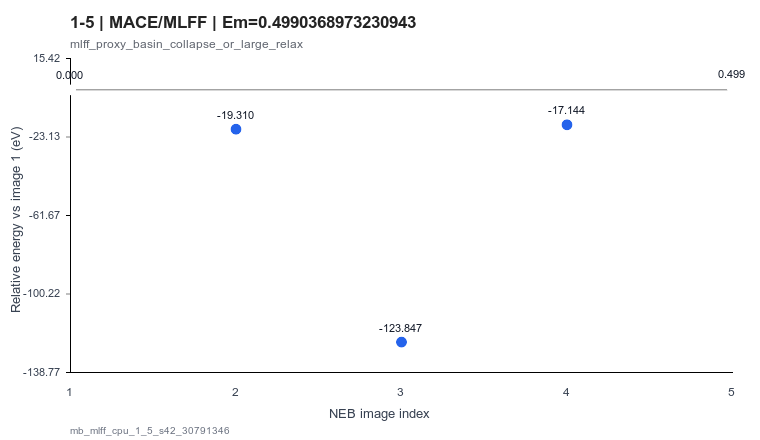
\includegraphics[width=\linewidth,height=0.42\textheight,keepaspectratio]{figure_pages/assets/fig_129.png}
\caption{Archived neb energy-profile or minimum-energy-path comparison. This page shows the candidate output ``05 1 5 mb mlff cpu 1 5 s42 30791346'' within the audited ARCHIVE-NEB-PROFILE family. The panel identity, source scope, and current status are retained in the accompanying evidence matrix.}
\label{fig:candidate_129}
\end{figure}
\textbf{Results text draft.} The profiles display the parsed path-level energy variation while preserving the distinction between reference candidates and formally converged paths. The plotted path identity is part of the evidence package.
\textbf{Discussion and boundary.} The figure supports qualitative path comparison and auditability. It must not imply final barrier accuracy for profiles that remain flagged as provisional or incomplete.
\textbf{Article placement.} Proposed article location: SI DFT NEB profiles / fixed-path benchmark.
\textbf{Reviewer linkage:} overall status PARTIAL.
\begin{itemize}[leftmargin=1.4em,noitemsep]
\item \textbf{REV-A1 (PARTIAL):} Reconcile Fig. 3d fixed-geometry DFT-path scoring with SI Fig. S3 self-consistent MLFF-NEB, including pathway identity and the DFT reference. \emph{Completed:} The fixed-path versus self-relaxed operator distinction and the narrower model-reported-barrier wording are integrated. \emph{Still required:} Close the restartable QE path-1--4 convergence gate, preserve the final path/source metadata, and complete the SI Fig. S3 endpoint/checkpoint/optimizer/source audit before calling the quantitative reference final.
\end{itemize}
\textbf{Evidence pointers.}
\begin{itemize}[leftmargin=1.4em,noitemsep]
\item Data/processed: \begingroup\scriptsize\url{paper/data/published/neb_energy_profiles/neb_energy_summary.csv}\endgroup
\item Data/processed: \begingroup\scriptsize\url{paper/data/published/neb_energy_profiles/neb_energy_summary.json}\endgroup
\item Caption/text source: \begingroup\scriptsize\url{paper/data/published/neb_energy_profiles/neb_energy_snapshot.md}\endgroup
\end{itemize}
\statusline{\textbf{Audit gap / next action:} No co-located plotting script; path-table provenance is present}
\vfill
\clearpage
\section{FIG-130 --- 06 1 6 mb mlff cpu 1 6 s42 30791347}
\label{figpage:fig-130}
\textbf{Group:} ARCHIVE-NEB-PROFILE\quad \textbf{Evidence chain:} partial\quad \textbf{Status:} publication;comparison
\begin{figure}[H]
\centering
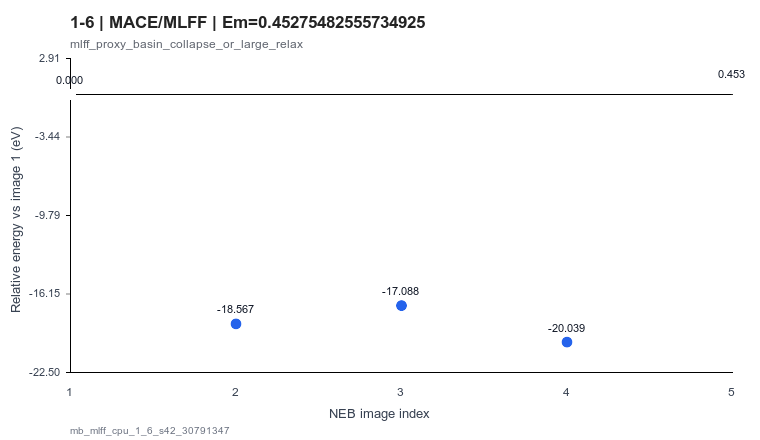
\includegraphics[width=\linewidth,height=0.42\textheight,keepaspectratio]{figure_pages/assets/fig_130.png}
\caption{Archived neb energy-profile or minimum-energy-path comparison. This page shows the candidate output ``06 1 6 mb mlff cpu 1 6 s42 30791347'' within the audited ARCHIVE-NEB-PROFILE family. The panel identity, source scope, and current status are retained in the accompanying evidence matrix.}
\label{fig:candidate_130}
\end{figure}
\textbf{Results text draft.} The profiles display the parsed path-level energy variation while preserving the distinction between reference candidates and formally converged paths. The plotted path identity is part of the evidence package.
\textbf{Discussion and boundary.} The figure supports qualitative path comparison and auditability. It must not imply final barrier accuracy for profiles that remain flagged as provisional or incomplete.
\textbf{Article placement.} Proposed article location: SI DFT NEB profiles / fixed-path benchmark.
\textbf{Reviewer linkage:} overall status PARTIAL.
\begin{itemize}[leftmargin=1.4em,noitemsep]
\item \textbf{REV-A1 (PARTIAL):} Reconcile Fig. 3d fixed-geometry DFT-path scoring with SI Fig. S3 self-consistent MLFF-NEB, including pathway identity and the DFT reference. \emph{Completed:} The fixed-path versus self-relaxed operator distinction and the narrower model-reported-barrier wording are integrated. \emph{Still required:} Close the restartable QE path-1--4 convergence gate, preserve the final path/source metadata, and complete the SI Fig. S3 endpoint/checkpoint/optimizer/source audit before calling the quantitative reference final.
\end{itemize}
\textbf{Evidence pointers.}
\begin{itemize}[leftmargin=1.4em,noitemsep]
\item Data/processed: \begingroup\scriptsize\url{paper/data/published/neb_energy_profiles/neb_energy_summary.csv}\endgroup
\item Data/processed: \begingroup\scriptsize\url{paper/data/published/neb_energy_profiles/neb_energy_summary.json}\endgroup
\item Caption/text source: \begingroup\scriptsize\url{paper/data/published/neb_energy_profiles/neb_energy_snapshot.md}\endgroup
\end{itemize}
\statusline{\textbf{Audit gap / next action:} No co-located plotting script; path-table provenance is present}
\vfill
\clearpage
\section{FIG-131 --- 07 1 6 mlff 1 6 repair idpp s42}
\label{figpage:fig-131}
\textbf{Group:} ARCHIVE-NEB-PROFILE\quad \textbf{Evidence chain:} partial\quad \textbf{Status:} publication;comparison
\begin{figure}[H]
\centering
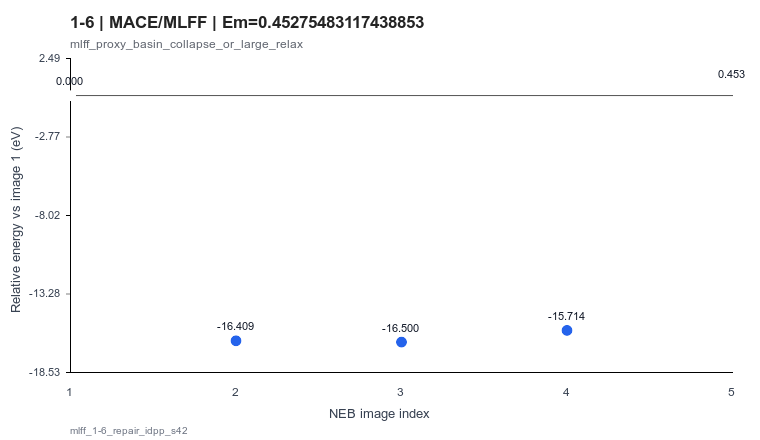
\includegraphics[width=\linewidth,height=0.42\textheight,keepaspectratio]{figure_pages/assets/fig_131.png}
\caption{Archived neb energy-profile or minimum-energy-path comparison. This page shows the candidate output ``07 1 6 mlff 1 6 repair idpp s42'' within the audited ARCHIVE-NEB-PROFILE family. The panel identity, source scope, and current status are retained in the accompanying evidence matrix.}
\label{fig:candidate_131}
\end{figure}
\textbf{Results text draft.} The profiles display the parsed path-level energy variation while preserving the distinction between reference candidates and formally converged paths. The plotted path identity is part of the evidence package.
\textbf{Discussion and boundary.} The figure supports qualitative path comparison and auditability. It must not imply final barrier accuracy for profiles that remain flagged as provisional or incomplete.
\textbf{Article placement.} Proposed article location: SI DFT NEB profiles / fixed-path benchmark.
\textbf{Reviewer linkage:} overall status PARTIAL.
\begin{itemize}[leftmargin=1.4em,noitemsep]
\item \textbf{REV-A1 (PARTIAL):} Reconcile Fig. 3d fixed-geometry DFT-path scoring with SI Fig. S3 self-consistent MLFF-NEB, including pathway identity and the DFT reference. \emph{Completed:} The fixed-path versus self-relaxed operator distinction and the narrower model-reported-barrier wording are integrated. \emph{Still required:} Close the restartable QE path-1--4 convergence gate, preserve the final path/source metadata, and complete the SI Fig. S3 endpoint/checkpoint/optimizer/source audit before calling the quantitative reference final.
\end{itemize}
\textbf{Evidence pointers.}
\begin{itemize}[leftmargin=1.4em,noitemsep]
\item Data/processed: \begingroup\scriptsize\url{paper/data/published/neb_energy_profiles/neb_energy_summary.csv}\endgroup
\item Data/processed: \begingroup\scriptsize\url{paper/data/published/neb_energy_profiles/neb_energy_summary.json}\endgroup
\item Caption/text source: \begingroup\scriptsize\url{paper/data/published/neb_energy_profiles/neb_energy_snapshot.md}\endgroup
\end{itemize}
\statusline{\textbf{Audit gap / next action:} No co-located plotting script; path-table provenance is present}
\vfill
\clearpage
\section{FIG-132 --- 08 1 6 mb qe16 direct pf s42 30791500}
\label{figpage:fig-132}
\textbf{Group:} ARCHIVE-NEB-PROFILE\quad \textbf{Evidence chain:} partial\quad \textbf{Status:} publication;comparison
\begin{figure}[H]
\centering
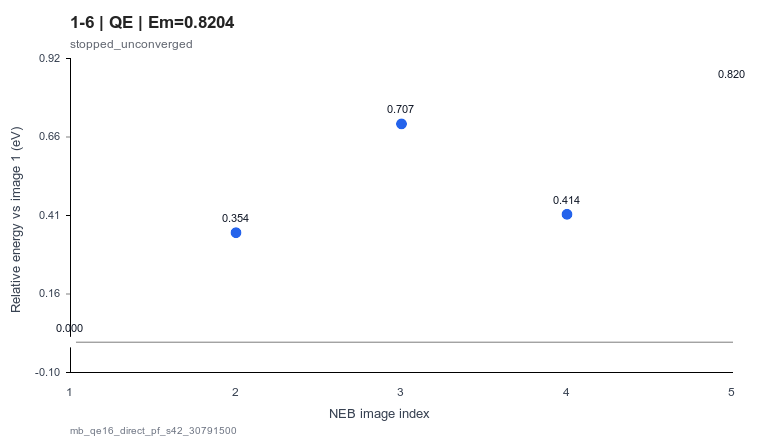
\includegraphics[width=\linewidth,height=0.42\textheight,keepaspectratio]{figure_pages/assets/fig_132.png}
\caption{Archived neb energy-profile or minimum-energy-path comparison. This page shows the candidate output ``08 1 6 mb qe16 direct pf s42 30791500'' within the audited ARCHIVE-NEB-PROFILE family. The panel identity, source scope, and current status are retained in the accompanying evidence matrix.}
\label{fig:candidate_132}
\end{figure}
\textbf{Results text draft.} The profiles display the parsed path-level energy variation while preserving the distinction between reference candidates and formally converged paths. The plotted path identity is part of the evidence package.
\textbf{Discussion and boundary.} The figure supports qualitative path comparison and auditability. It must not imply final barrier accuracy for profiles that remain flagged as provisional or incomplete.
\textbf{Article placement.} Proposed article location: SI DFT NEB profiles / fixed-path benchmark.
\textbf{Reviewer linkage:} overall status PARTIAL.
\begin{itemize}[leftmargin=1.4em,noitemsep]
\item \textbf{REV-A1 (PARTIAL):} Reconcile Fig. 3d fixed-geometry DFT-path scoring with SI Fig. S3 self-consistent MLFF-NEB, including pathway identity and the DFT reference. \emph{Completed:} The fixed-path versus self-relaxed operator distinction and the narrower model-reported-barrier wording are integrated. \emph{Still required:} Close the restartable QE path-1--4 convergence gate, preserve the final path/source metadata, and complete the SI Fig. S3 endpoint/checkpoint/optimizer/source audit before calling the quantitative reference final.
\end{itemize}
\textbf{Evidence pointers.}
\begin{itemize}[leftmargin=1.4em,noitemsep]
\item Data/processed: \begingroup\scriptsize\url{paper/data/published/neb_energy_profiles/neb_energy_summary.csv}\endgroup
\item Data/processed: \begingroup\scriptsize\url{paper/data/published/neb_energy_profiles/neb_energy_summary.json}\endgroup
\item Caption/text source: \begingroup\scriptsize\url{paper/data/published/neb_energy_profiles/neb_energy_snapshot.md}\endgroup
\end{itemize}
\statusline{\textbf{Audit gap / next action:} No co-located plotting script; path-table provenance is present}
\vfill
\clearpage
\section{FIG-133 --- 09 1 6 mb qe16 direct r2 s42 30791828}
\label{figpage:fig-133}
\textbf{Group:} ARCHIVE-NEB-PROFILE\quad \textbf{Evidence chain:} partial\quad \textbf{Status:} publication;comparison
\begin{figure}[H]
\centering
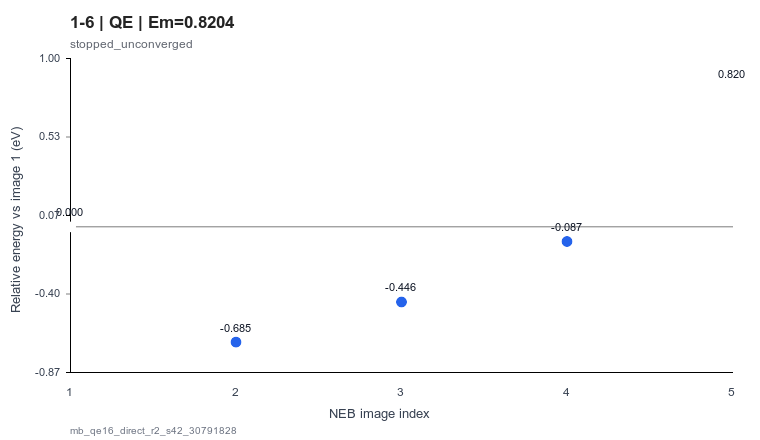
\includegraphics[width=\linewidth,height=0.42\textheight,keepaspectratio]{figure_pages/assets/fig_133.png}
\caption{Archived neb energy-profile or minimum-energy-path comparison. This page shows the candidate output ``09 1 6 mb qe16 direct r2 s42 30791828'' within the audited ARCHIVE-NEB-PROFILE family. The panel identity, source scope, and current status are retained in the accompanying evidence matrix.}
\label{fig:candidate_133}
\end{figure}
\textbf{Results text draft.} The profiles display the parsed path-level energy variation while preserving the distinction between reference candidates and formally converged paths. The plotted path identity is part of the evidence package.
\textbf{Discussion and boundary.} The figure supports qualitative path comparison and auditability. It must not imply final barrier accuracy for profiles that remain flagged as provisional or incomplete.
\textbf{Article placement.} Proposed article location: SI DFT NEB profiles / fixed-path benchmark.
\textbf{Reviewer linkage:} overall status PARTIAL.
\begin{itemize}[leftmargin=1.4em,noitemsep]
\item \textbf{REV-A1 (PARTIAL):} Reconcile Fig. 3d fixed-geometry DFT-path scoring with SI Fig. S3 self-consistent MLFF-NEB, including pathway identity and the DFT reference. \emph{Completed:} The fixed-path versus self-relaxed operator distinction and the narrower model-reported-barrier wording are integrated. \emph{Still required:} Close the restartable QE path-1--4 convergence gate, preserve the final path/source metadata, and complete the SI Fig. S3 endpoint/checkpoint/optimizer/source audit before calling the quantitative reference final.
\end{itemize}
\textbf{Evidence pointers.}
\begin{itemize}[leftmargin=1.4em,noitemsep]
\item Data/processed: \begingroup\scriptsize\url{paper/data/published/neb_energy_profiles/neb_energy_summary.csv}\endgroup
\item Data/processed: \begingroup\scriptsize\url{paper/data/published/neb_energy_profiles/neb_energy_summary.json}\endgroup
\item Caption/text source: \begingroup\scriptsize\url{paper/data/published/neb_energy_profiles/neb_energy_snapshot.md}\endgroup
\end{itemize}
\statusline{\textbf{Audit gap / next action:} No co-located plotting script; path-table provenance is present}
\vfill
\clearpage
\section{FIG-134 --- 10 1 6 mb qe16 direct r3 s42 30812496}
\label{figpage:fig-134}
\textbf{Group:} ARCHIVE-NEB-PROFILE\quad \textbf{Evidence chain:} partial\quad \textbf{Status:} publication;comparison
\begin{figure}[H]
\centering
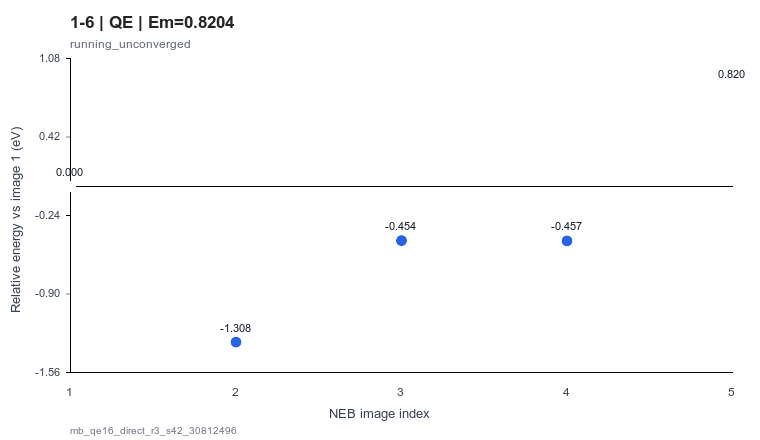
\includegraphics[width=\linewidth,height=0.42\textheight,keepaspectratio]{figure_pages/assets/fig_134.png}
\caption{Archived neb energy-profile or minimum-energy-path comparison. This page shows the candidate output ``10 1 6 mb qe16 direct r3 s42 30812496'' within the audited ARCHIVE-NEB-PROFILE family. The panel identity, source scope, and current status are retained in the accompanying evidence matrix.}
\label{fig:candidate_134}
\end{figure}
\textbf{Results text draft.} The profiles display the parsed path-level energy variation while preserving the distinction between reference candidates and formally converged paths. The plotted path identity is part of the evidence package.
\textbf{Discussion and boundary.} The figure supports qualitative path comparison and auditability. It must not imply final barrier accuracy for profiles that remain flagged as provisional or incomplete.
\textbf{Article placement.} Proposed article location: SI DFT NEB profiles / fixed-path benchmark.
\textbf{Reviewer linkage:} overall status PARTIAL.
\begin{itemize}[leftmargin=1.4em,noitemsep]
\item \textbf{REV-A1 (PARTIAL):} Reconcile Fig. 3d fixed-geometry DFT-path scoring with SI Fig. S3 self-consistent MLFF-NEB, including pathway identity and the DFT reference. \emph{Completed:} The fixed-path versus self-relaxed operator distinction and the narrower model-reported-barrier wording are integrated. \emph{Still required:} Close the restartable QE path-1--4 convergence gate, preserve the final path/source metadata, and complete the SI Fig. S3 endpoint/checkpoint/optimizer/source audit before calling the quantitative reference final.
\end{itemize}
\textbf{Evidence pointers.}
\begin{itemize}[leftmargin=1.4em,noitemsep]
\item Data/processed: \begingroup\scriptsize\url{paper/data/published/neb_energy_profiles/neb_energy_summary.csv}\endgroup
\item Data/processed: \begingroup\scriptsize\url{paper/data/published/neb_energy_profiles/neb_energy_summary.json}\endgroup
\item Caption/text source: \begingroup\scriptsize\url{paper/data/published/neb_energy_profiles/neb_energy_snapshot.md}\endgroup
\end{itemize}
\statusline{\textbf{Audit gap / next action:} No co-located plotting script; path-table provenance is present}
\vfill
\clearpage
\section{FIG-135 --- 12 1 7 mb qe17 direct pf s42 30791508}
\label{figpage:fig-135}
\textbf{Group:} ARCHIVE-NEB-PROFILE\quad \textbf{Evidence chain:} partial\quad \textbf{Status:} publication;comparison
\begin{figure}[H]
\centering
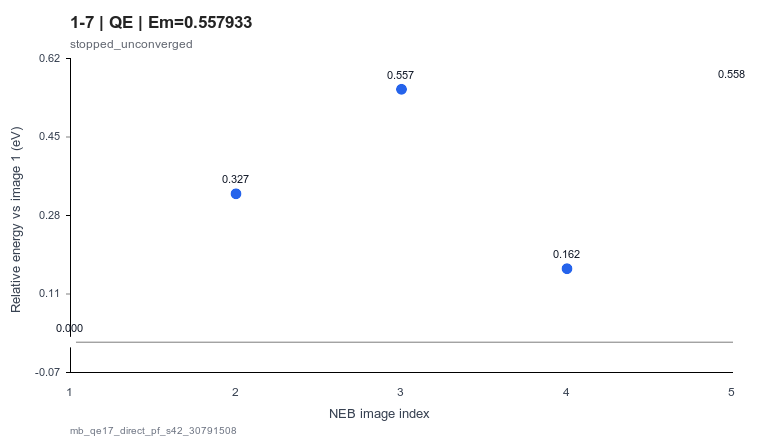
\includegraphics[width=\linewidth,height=0.42\textheight,keepaspectratio]{figure_pages/assets/fig_135.png}
\caption{Archived neb energy-profile or minimum-energy-path comparison. This page shows the candidate output ``12 1 7 mb qe17 direct pf s42 30791508'' within the audited ARCHIVE-NEB-PROFILE family. The panel identity, source scope, and current status are retained in the accompanying evidence matrix.}
\label{fig:candidate_135}
\end{figure}
\textbf{Results text draft.} The profiles display the parsed path-level energy variation while preserving the distinction between reference candidates and formally converged paths. The plotted path identity is part of the evidence package.
\textbf{Discussion and boundary.} The figure supports qualitative path comparison and auditability. It must not imply final barrier accuracy for profiles that remain flagged as provisional or incomplete.
\textbf{Article placement.} Proposed article location: SI DFT NEB profiles / fixed-path benchmark.
\textbf{Reviewer linkage:} overall status PARTIAL.
\begin{itemize}[leftmargin=1.4em,noitemsep]
\item \textbf{REV-A1 (PARTIAL):} Reconcile Fig. 3d fixed-geometry DFT-path scoring with SI Fig. S3 self-consistent MLFF-NEB, including pathway identity and the DFT reference. \emph{Completed:} The fixed-path versus self-relaxed operator distinction and the narrower model-reported-barrier wording are integrated. \emph{Still required:} Close the restartable QE path-1--4 convergence gate, preserve the final path/source metadata, and complete the SI Fig. S3 endpoint/checkpoint/optimizer/source audit before calling the quantitative reference final.
\end{itemize}
\textbf{Evidence pointers.}
\begin{itemize}[leftmargin=1.4em,noitemsep]
\item Data/processed: \begingroup\scriptsize\url{paper/data/published/neb_energy_profiles/neb_energy_summary.csv}\endgroup
\item Data/processed: \begingroup\scriptsize\url{paper/data/published/neb_energy_profiles/neb_energy_summary.json}\endgroup
\item Caption/text source: \begingroup\scriptsize\url{paper/data/published/neb_energy_profiles/neb_energy_snapshot.md}\endgroup
\end{itemize}
\statusline{\textbf{Audit gap / next action:} No co-located plotting script; path-table provenance is present}
\vfill
\clearpage
\section{FIG-136 --- 13 1 7 mb qe17 direct r2 s42 30791829}
\label{figpage:fig-136}
\textbf{Group:} ARCHIVE-NEB-PROFILE\quad \textbf{Evidence chain:} partial\quad \textbf{Status:} publication;comparison
\begin{figure}[H]
\centering
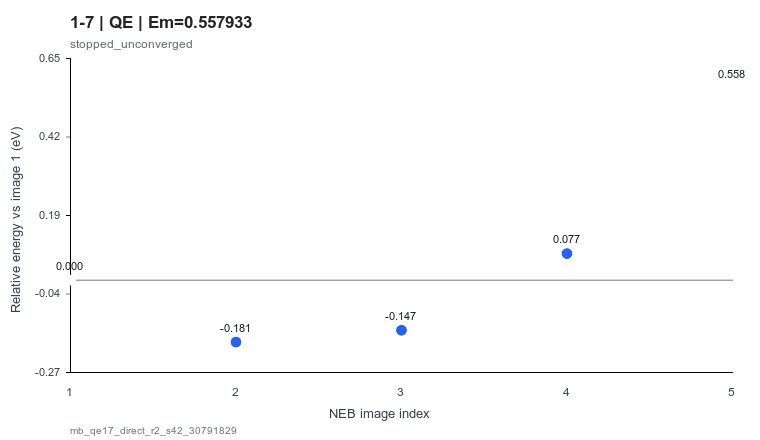
\includegraphics[width=\linewidth,height=0.42\textheight,keepaspectratio]{figure_pages/assets/fig_136.png}
\caption{Archived neb energy-profile or minimum-energy-path comparison. This page shows the candidate output ``13 1 7 mb qe17 direct r2 s42 30791829'' within the audited ARCHIVE-NEB-PROFILE family. The panel identity, source scope, and current status are retained in the accompanying evidence matrix.}
\label{fig:candidate_136}
\end{figure}
\textbf{Results text draft.} The profiles display the parsed path-level energy variation while preserving the distinction between reference candidates and formally converged paths. The plotted path identity is part of the evidence package.
\textbf{Discussion and boundary.} The figure supports qualitative path comparison and auditability. It must not imply final barrier accuracy for profiles that remain flagged as provisional or incomplete.
\textbf{Article placement.} Proposed article location: SI DFT NEB profiles / fixed-path benchmark.
\textbf{Reviewer linkage:} overall status PARTIAL.
\begin{itemize}[leftmargin=1.4em,noitemsep]
\item \textbf{REV-A1 (PARTIAL):} Reconcile Fig. 3d fixed-geometry DFT-path scoring with SI Fig. S3 self-consistent MLFF-NEB, including pathway identity and the DFT reference. \emph{Completed:} The fixed-path versus self-relaxed operator distinction and the narrower model-reported-barrier wording are integrated. \emph{Still required:} Close the restartable QE path-1--4 convergence gate, preserve the final path/source metadata, and complete the SI Fig. S3 endpoint/checkpoint/optimizer/source audit before calling the quantitative reference final.
\end{itemize}
\textbf{Evidence pointers.}
\begin{itemize}[leftmargin=1.4em,noitemsep]
\item Data/processed: \begingroup\scriptsize\url{paper/data/published/neb_energy_profiles/neb_energy_summary.csv}\endgroup
\item Data/processed: \begingroup\scriptsize\url{paper/data/published/neb_energy_profiles/neb_energy_summary.json}\endgroup
\item Caption/text source: \begingroup\scriptsize\url{paper/data/published/neb_energy_profiles/neb_energy_snapshot.md}\endgroup
\end{itemize}
\statusline{\textbf{Audit gap / next action:} No co-located plotting script; path-table provenance is present}
\vfill
\clearpage
\section{FIG-137 --- 14 1 7 mb qe17 direct r3 s42 30812497}
\label{figpage:fig-137}
\textbf{Group:} ARCHIVE-NEB-PROFILE\quad \textbf{Evidence chain:} partial\quad \textbf{Status:} publication;comparison
\begin{figure}[H]
\centering
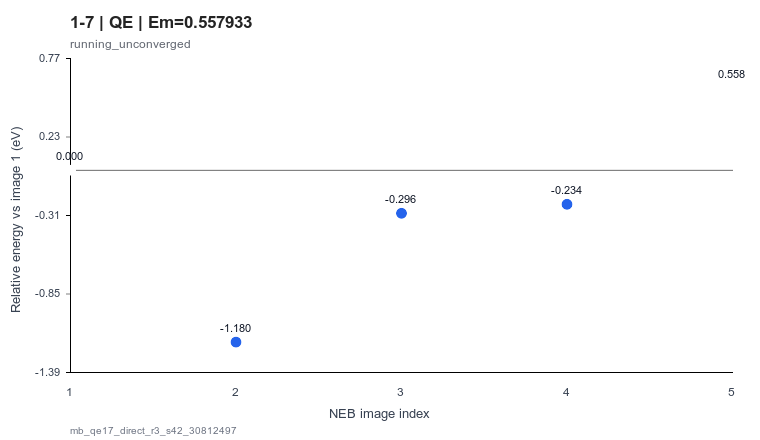
\includegraphics[width=\linewidth,height=0.42\textheight,keepaspectratio]{figure_pages/assets/fig_137.png}
\caption{Archived neb energy-profile or minimum-energy-path comparison. This page shows the candidate output ``14 1 7 mb qe17 direct r3 s42 30812497'' within the audited ARCHIVE-NEB-PROFILE family. The panel identity, source scope, and current status are retained in the accompanying evidence matrix.}
\label{fig:candidate_137}
\end{figure}
\textbf{Results text draft.} The profiles display the parsed path-level energy variation while preserving the distinction between reference candidates and formally converged paths. The plotted path identity is part of the evidence package.
\textbf{Discussion and boundary.} The figure supports qualitative path comparison and auditability. It must not imply final barrier accuracy for profiles that remain flagged as provisional or incomplete.
\textbf{Article placement.} Proposed article location: SI DFT NEB profiles / fixed-path benchmark.
\textbf{Reviewer linkage:} overall status PARTIAL.
\begin{itemize}[leftmargin=1.4em,noitemsep]
\item \textbf{REV-A1 (PARTIAL):} Reconcile Fig. 3d fixed-geometry DFT-path scoring with SI Fig. S3 self-consistent MLFF-NEB, including pathway identity and the DFT reference. \emph{Completed:} The fixed-path versus self-relaxed operator distinction and the narrower model-reported-barrier wording are integrated. \emph{Still required:} Close the restartable QE path-1--4 convergence gate, preserve the final path/source metadata, and complete the SI Fig. S3 endpoint/checkpoint/optimizer/source audit before calling the quantitative reference final.
\end{itemize}
\textbf{Evidence pointers.}
\begin{itemize}[leftmargin=1.4em,noitemsep]
\item Data/processed: \begingroup\scriptsize\url{paper/data/published/neb_energy_profiles/neb_energy_summary.csv}\endgroup
\item Data/processed: \begingroup\scriptsize\url{paper/data/published/neb_energy_profiles/neb_energy_summary.json}\endgroup
\item Caption/text source: \begingroup\scriptsize\url{paper/data/published/neb_energy_profiles/neb_energy_snapshot.md}\endgroup
\end{itemize}
\statusline{\textbf{Audit gap / next action:} No co-located plotting script; path-table provenance is present}
\vfill
\clearpage
\section{FIG-138 --- 19 81 neb 1 historical 2d 421 neb 1}
\label{figpage:fig-138}
\textbf{Group:} ARCHIVE-NEB-PROFILE\quad \textbf{Evidence chain:} partial\quad \textbf{Status:} publication;old\_or\_legacy;comparison
\begin{figure}[H]
\centering
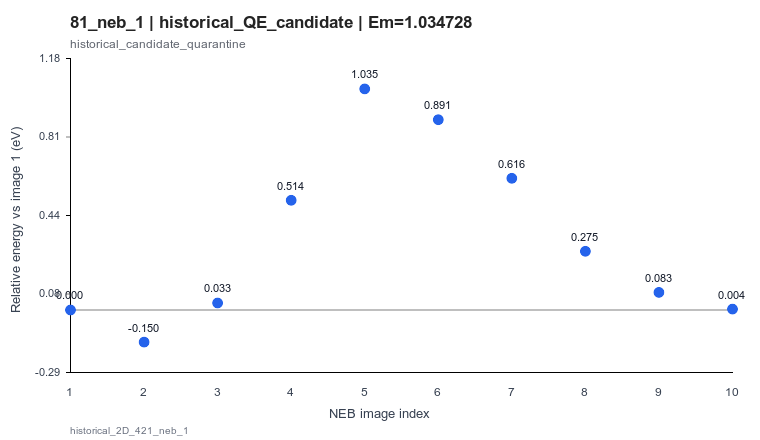
\includegraphics[width=\linewidth,height=0.42\textheight,keepaspectratio]{figure_pages/assets/fig_138.png}
\caption{Archived neb energy-profile or minimum-energy-path comparison. This page shows the candidate output ``19 81 neb 1 historical 2d 421 neb 1'' within the audited ARCHIVE-NEB-PROFILE family. The panel identity, source scope, and current status are retained in the accompanying evidence matrix.}
\label{fig:candidate_138}
\end{figure}
\textbf{Results text draft.} The profiles display the parsed path-level energy variation while preserving the distinction between reference candidates and formally converged paths. The plotted path identity is part of the evidence package.
\textbf{Discussion and boundary.} The figure supports qualitative path comparison and auditability. It must not imply final barrier accuracy for profiles that remain flagged as provisional or incomplete.
\textbf{Article placement.} Proposed article location: SI DFT NEB profiles / fixed-path benchmark.
\textbf{Reviewer linkage:} overall status PARTIAL.
\begin{itemize}[leftmargin=1.4em,noitemsep]
\item \textbf{REV-A1 (PARTIAL):} Reconcile Fig. 3d fixed-geometry DFT-path scoring with SI Fig. S3 self-consistent MLFF-NEB, including pathway identity and the DFT reference. \emph{Completed:} The fixed-path versus self-relaxed operator distinction and the narrower model-reported-barrier wording are integrated. \emph{Still required:} Close the restartable QE path-1--4 convergence gate, preserve the final path/source metadata, and complete the SI Fig. S3 endpoint/checkpoint/optimizer/source audit before calling the quantitative reference final.
\end{itemize}
\textbf{Evidence pointers.}
\begin{itemize}[leftmargin=1.4em,noitemsep]
\item Data/processed: \begingroup\scriptsize\url{paper/data/published/neb_energy_profiles/neb_energy_summary.csv}\endgroup
\item Data/processed: \begingroup\scriptsize\url{paper/data/published/neb_energy_profiles/neb_energy_summary.json}\endgroup
\item Caption/text source: \begingroup\scriptsize\url{paper/data/published/neb_energy_profiles/neb_energy_snapshot.md}\endgroup
\end{itemize}
\statusline{\textbf{Audit gap / next action:} No co-located plotting script; path-table provenance is present}
\vfill
\clearpage
\section{FIG-139 --- 20 81 neb 2 historical 2d 421 neb 2}
\label{figpage:fig-139}
\textbf{Group:} ARCHIVE-NEB-PROFILE\quad \textbf{Evidence chain:} partial\quad \textbf{Status:} publication;old\_or\_legacy;comparison
\begin{figure}[H]
\centering
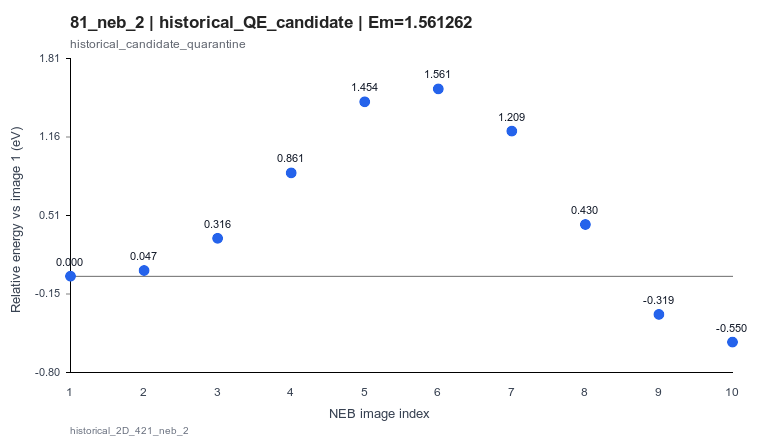
\includegraphics[width=\linewidth,height=0.42\textheight,keepaspectratio]{figure_pages/assets/fig_139.png}
\caption{Archived neb energy-profile or minimum-energy-path comparison. This page shows the candidate output ``20 81 neb 2 historical 2d 421 neb 2'' within the audited ARCHIVE-NEB-PROFILE family. The panel identity, source scope, and current status are retained in the accompanying evidence matrix.}
\label{fig:candidate_139}
\end{figure}
\textbf{Results text draft.} The profiles display the parsed path-level energy variation while preserving the distinction between reference candidates and formally converged paths. The plotted path identity is part of the evidence package.
\textbf{Discussion and boundary.} The figure supports qualitative path comparison and auditability. It must not imply final barrier accuracy for profiles that remain flagged as provisional or incomplete.
\textbf{Article placement.} Proposed article location: SI DFT NEB profiles / fixed-path benchmark.
\textbf{Reviewer linkage:} overall status PARTIAL.
\begin{itemize}[leftmargin=1.4em,noitemsep]
\item \textbf{REV-A1 (PARTIAL):} Reconcile Fig. 3d fixed-geometry DFT-path scoring with SI Fig. S3 self-consistent MLFF-NEB, including pathway identity and the DFT reference. \emph{Completed:} The fixed-path versus self-relaxed operator distinction and the narrower model-reported-barrier wording are integrated. \emph{Still required:} Close the restartable QE path-1--4 convergence gate, preserve the final path/source metadata, and complete the SI Fig. S3 endpoint/checkpoint/optimizer/source audit before calling the quantitative reference final.
\end{itemize}
\textbf{Evidence pointers.}
\begin{itemize}[leftmargin=1.4em,noitemsep]
\item Data/processed: \begingroup\scriptsize\url{paper/data/published/neb_energy_profiles/neb_energy_summary.csv}\endgroup
\item Data/processed: \begingroup\scriptsize\url{paper/data/published/neb_energy_profiles/neb_energy_summary.json}\endgroup
\item Caption/text source: \begingroup\scriptsize\url{paper/data/published/neb_energy_profiles/neb_energy_snapshot.md}\endgroup
\end{itemize}
\statusline{\textbf{Audit gap / next action:} No co-located plotting script; path-table provenance is present}
\vfill
\clearpage
\section{FIG-140 --- 21 81 neb 3 historical 2d 421 neb 3}
\label{figpage:fig-140}
\textbf{Group:} ARCHIVE-NEB-PROFILE\quad \textbf{Evidence chain:} partial\quad \textbf{Status:} publication;old\_or\_legacy;comparison
\begin{figure}[H]
\centering
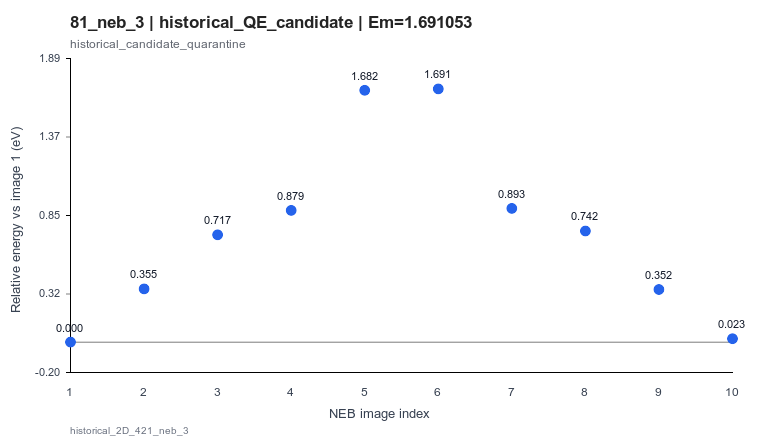
\includegraphics[width=\linewidth,height=0.42\textheight,keepaspectratio]{figure_pages/assets/fig_140.png}
\caption{Archived neb energy-profile or minimum-energy-path comparison. This page shows the candidate output ``21 81 neb 3 historical 2d 421 neb 3'' within the audited ARCHIVE-NEB-PROFILE family. The panel identity, source scope, and current status are retained in the accompanying evidence matrix.}
\label{fig:candidate_140}
\end{figure}
\textbf{Results text draft.} The profiles display the parsed path-level energy variation while preserving the distinction between reference candidates and formally converged paths. The plotted path identity is part of the evidence package.
\textbf{Discussion and boundary.} The figure supports qualitative path comparison and auditability. It must not imply final barrier accuracy for profiles that remain flagged as provisional or incomplete.
\textbf{Article placement.} Proposed article location: SI DFT NEB profiles / fixed-path benchmark.
\textbf{Reviewer linkage:} overall status PARTIAL.
\begin{itemize}[leftmargin=1.4em,noitemsep]
\item \textbf{REV-A1 (PARTIAL):} Reconcile Fig. 3d fixed-geometry DFT-path scoring with SI Fig. S3 self-consistent MLFF-NEB, including pathway identity and the DFT reference. \emph{Completed:} The fixed-path versus self-relaxed operator distinction and the narrower model-reported-barrier wording are integrated. \emph{Still required:} Close the restartable QE path-1--4 convergence gate, preserve the final path/source metadata, and complete the SI Fig. S3 endpoint/checkpoint/optimizer/source audit before calling the quantitative reference final.
\end{itemize}
\textbf{Evidence pointers.}
\begin{itemize}[leftmargin=1.4em,noitemsep]
\item Data/processed: \begingroup\scriptsize\url{paper/data/published/neb_energy_profiles/neb_energy_summary.csv}\endgroup
\item Data/processed: \begingroup\scriptsize\url{paper/data/published/neb_energy_profiles/neb_energy_summary.json}\endgroup
\item Caption/text source: \begingroup\scriptsize\url{paper/data/published/neb_energy_profiles/neb_energy_snapshot.md}\endgroup
\end{itemize}
\statusline{\textbf{Audit gap / next action:} No co-located plotting script; path-table provenance is present}
\vfill
\clearpage
\section{FIG-141 --- 23 81 neb 4 historical 2d 421 neb 4}
\label{figpage:fig-141}
\textbf{Group:} ARCHIVE-NEB-PROFILE\quad \textbf{Evidence chain:} partial\quad \textbf{Status:} publication;old\_or\_legacy;comparison
\begin{figure}[H]
\centering
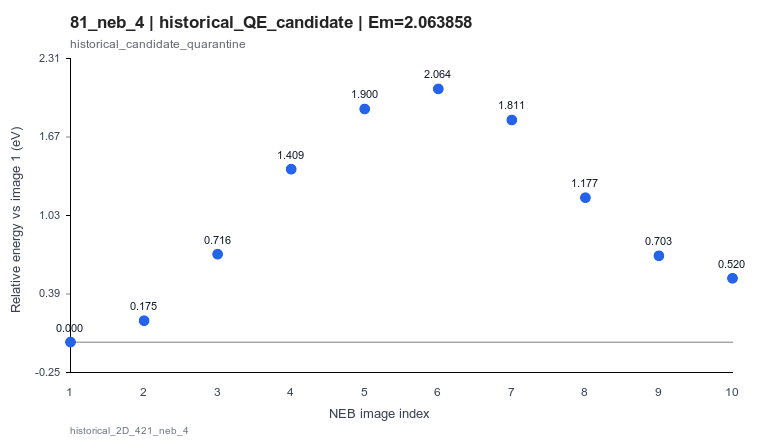
\includegraphics[width=\linewidth,height=0.42\textheight,keepaspectratio]{figure_pages/assets/fig_141.png}
\caption{Archived neb energy-profile or minimum-energy-path comparison. This page shows the candidate output ``23 81 neb 4 historical 2d 421 neb 4'' within the audited ARCHIVE-NEB-PROFILE family. The panel identity, source scope, and current status are retained in the accompanying evidence matrix.}
\label{fig:candidate_141}
\end{figure}
\textbf{Results text draft.} The profiles display the parsed path-level energy variation while preserving the distinction between reference candidates and formally converged paths. The plotted path identity is part of the evidence package.
\textbf{Discussion and boundary.} The figure supports qualitative path comparison and auditability. It must not imply final barrier accuracy for profiles that remain flagged as provisional or incomplete.
\textbf{Article placement.} Proposed article location: SI DFT NEB profiles / fixed-path benchmark.
\textbf{Reviewer linkage:} overall status PARTIAL.
\begin{itemize}[leftmargin=1.4em,noitemsep]
\item \textbf{REV-A1 (PARTIAL):} Reconcile Fig. 3d fixed-geometry DFT-path scoring with SI Fig. S3 self-consistent MLFF-NEB, including pathway identity and the DFT reference. \emph{Completed:} The fixed-path versus self-relaxed operator distinction and the narrower model-reported-barrier wording are integrated. \emph{Still required:} Close the restartable QE path-1--4 convergence gate, preserve the final path/source metadata, and complete the SI Fig. S3 endpoint/checkpoint/optimizer/source audit before calling the quantitative reference final.
\end{itemize}
\textbf{Evidence pointers.}
\begin{itemize}[leftmargin=1.4em,noitemsep]
\item Data/processed: \begingroup\scriptsize\url{paper/data/published/neb_energy_profiles/neb_energy_summary.csv}\endgroup
\item Data/processed: \begingroup\scriptsize\url{paper/data/published/neb_energy_profiles/neb_energy_summary.json}\endgroup
\item Caption/text source: \begingroup\scriptsize\url{paper/data/published/neb_energy_profiles/neb_energy_snapshot.md}\endgroup
\end{itemize}
\statusline{\textbf{Audit gap / next action:} No co-located plotting script; path-table provenance is present}
\vfill
\clearpage
\section{FIG-142 --- 24 81 neb 5 historical 2d 421 neb 5}
\label{figpage:fig-142}
\textbf{Group:} ARCHIVE-NEB-PROFILE\quad \textbf{Evidence chain:} partial\quad \textbf{Status:} publication;old\_or\_legacy;comparison
\begin{figure}[H]
\centering
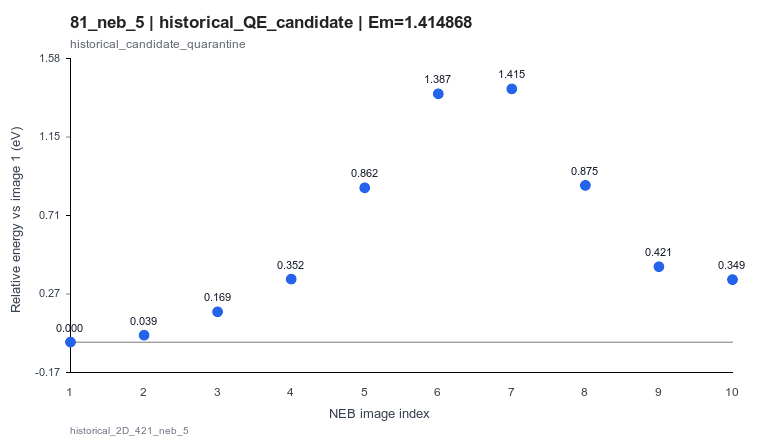
\includegraphics[width=\linewidth,height=0.42\textheight,keepaspectratio]{figure_pages/assets/fig_142.png}
\caption{Archived neb energy-profile or minimum-energy-path comparison. This page shows the candidate output ``24 81 neb 5 historical 2d 421 neb 5'' within the audited ARCHIVE-NEB-PROFILE family. The panel identity, source scope, and current status are retained in the accompanying evidence matrix.}
\label{fig:candidate_142}
\end{figure}
\textbf{Results text draft.} The profiles display the parsed path-level energy variation while preserving the distinction between reference candidates and formally converged paths. The plotted path identity is part of the evidence package.
\textbf{Discussion and boundary.} The figure supports qualitative path comparison and auditability. It must not imply final barrier accuracy for profiles that remain flagged as provisional or incomplete.
\textbf{Article placement.} Proposed article location: SI DFT NEB profiles / fixed-path benchmark.
\textbf{Reviewer linkage:} overall status PARTIAL.
\begin{itemize}[leftmargin=1.4em,noitemsep]
\item \textbf{REV-A1 (PARTIAL):} Reconcile Fig. 3d fixed-geometry DFT-path scoring with SI Fig. S3 self-consistent MLFF-NEB, including pathway identity and the DFT reference. \emph{Completed:} The fixed-path versus self-relaxed operator distinction and the narrower model-reported-barrier wording are integrated. \emph{Still required:} Close the restartable QE path-1--4 convergence gate, preserve the final path/source metadata, and complete the SI Fig. S3 endpoint/checkpoint/optimizer/source audit before calling the quantitative reference final.
\end{itemize}
\textbf{Evidence pointers.}
\begin{itemize}[leftmargin=1.4em,noitemsep]
\item Data/processed: \begingroup\scriptsize\url{paper/data/published/neb_energy_profiles/neb_energy_summary.csv}\endgroup
\item Data/processed: \begingroup\scriptsize\url{paper/data/published/neb_energy_profiles/neb_energy_summary.json}\endgroup
\item Caption/text source: \begingroup\scriptsize\url{paper/data/published/neb_energy_profiles/neb_energy_snapshot.md}\endgroup
\end{itemize}
\statusline{\textbf{Audit gap / next action:} No co-located plotting script; path-table provenance is present}
\vfill
\clearpage
\section{FIG-143 --- 27 victor neb2 victor historical v st neb2}
\label{figpage:fig-143}
\textbf{Group:} ARCHIVE-NEB-PROFILE\quad \textbf{Evidence chain:} partial\quad \textbf{Status:} publication;old\_or\_legacy;comparison
\begin{figure}[H]
\centering
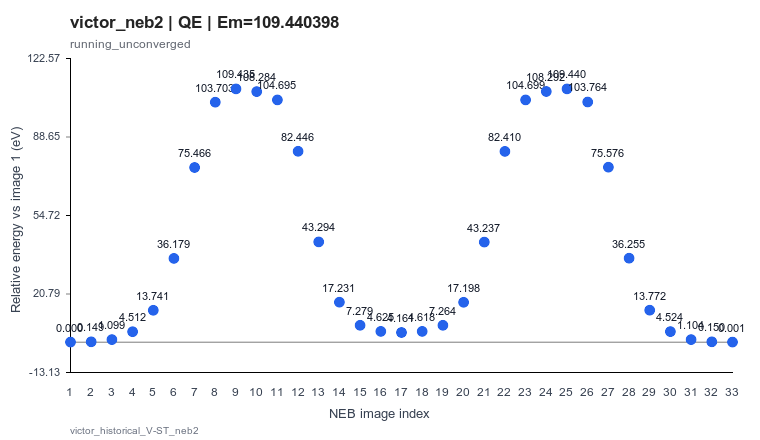
\includegraphics[width=\linewidth,height=0.42\textheight,keepaspectratio]{figure_pages/assets/fig_143.png}
\caption{Archived neb energy-profile or minimum-energy-path comparison. This page shows the candidate output ``27 victor neb2 victor historical v st neb2'' within the audited ARCHIVE-NEB-PROFILE family. The panel identity, source scope, and current status are retained in the accompanying evidence matrix.}
\label{fig:candidate_143}
\end{figure}
\textbf{Results text draft.} The profiles display the parsed path-level energy variation while preserving the distinction between reference candidates and formally converged paths. The plotted path identity is part of the evidence package.
\textbf{Discussion and boundary.} The figure supports qualitative path comparison and auditability. It must not imply final barrier accuracy for profiles that remain flagged as provisional or incomplete.
\textbf{Article placement.} Proposed article location: SI DFT NEB profiles / fixed-path benchmark.
\textbf{Reviewer linkage:} overall status PARTIAL.
\begin{itemize}[leftmargin=1.4em,noitemsep]
\item \textbf{REV-A1 (PARTIAL):} Reconcile Fig. 3d fixed-geometry DFT-path scoring with SI Fig. S3 self-consistent MLFF-NEB, including pathway identity and the DFT reference. \emph{Completed:} The fixed-path versus self-relaxed operator distinction and the narrower model-reported-barrier wording are integrated. \emph{Still required:} Close the restartable QE path-1--4 convergence gate, preserve the final path/source metadata, and complete the SI Fig. S3 endpoint/checkpoint/optimizer/source audit before calling the quantitative reference final.
\end{itemize}
\textbf{Evidence pointers.}
\begin{itemize}[leftmargin=1.4em,noitemsep]
\item Data/processed: \begingroup\scriptsize\url{paper/data/published/neb_energy_profiles/neb_energy_summary.csv}\endgroup
\item Data/processed: \begingroup\scriptsize\url{paper/data/published/neb_energy_profiles/neb_energy_summary.json}\endgroup
\item Caption/text source: \begingroup\scriptsize\url{paper/data/published/neb_energy_profiles/neb_energy_snapshot.md}\endgroup
\end{itemize}
\statusline{\textbf{Audit gap / next action:} No co-located plotting script; path-table provenance is present}
\vfill
\clearpage
\section{FIG-144 --- 28 victor neb2 copy victor historical v st neb2 copy}
\label{figpage:fig-144}
\textbf{Group:} ARCHIVE-NEB-PROFILE\quad \textbf{Evidence chain:} partial\quad \textbf{Status:} publication;old\_or\_legacy;comparison
\begin{figure}[H]
\centering
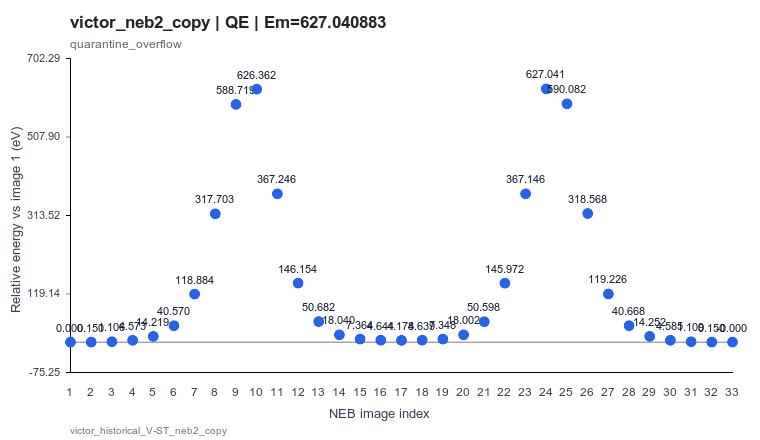
\includegraphics[width=\linewidth,height=0.42\textheight,keepaspectratio]{figure_pages/assets/fig_144.png}
\caption{Archived neb energy-profile or minimum-energy-path comparison. This page shows the candidate output ``28 victor neb2 copy victor historical v st neb2 copy'' within the audited ARCHIVE-NEB-PROFILE family. The panel identity, source scope, and current status are retained in the accompanying evidence matrix.}
\label{fig:candidate_144}
\end{figure}
\textbf{Results text draft.} The profiles display the parsed path-level energy variation while preserving the distinction between reference candidates and formally converged paths. The plotted path identity is part of the evidence package.
\textbf{Discussion and boundary.} The figure supports qualitative path comparison and auditability. It must not imply final barrier accuracy for profiles that remain flagged as provisional or incomplete.
\textbf{Article placement.} Proposed article location: SI DFT NEB profiles / fixed-path benchmark.
\textbf{Reviewer linkage:} overall status PARTIAL.
\begin{itemize}[leftmargin=1.4em,noitemsep]
\item \textbf{REV-A1 (PARTIAL):} Reconcile Fig. 3d fixed-geometry DFT-path scoring with SI Fig. S3 self-consistent MLFF-NEB, including pathway identity and the DFT reference. \emph{Completed:} The fixed-path versus self-relaxed operator distinction and the narrower model-reported-barrier wording are integrated. \emph{Still required:} Close the restartable QE path-1--4 convergence gate, preserve the final path/source metadata, and complete the SI Fig. S3 endpoint/checkpoint/optimizer/source audit before calling the quantitative reference final.
\end{itemize}
\textbf{Evidence pointers.}
\begin{itemize}[leftmargin=1.4em,noitemsep]
\item Data/processed: \begingroup\scriptsize\url{paper/data/published/neb_energy_profiles/neb_energy_summary.csv}\endgroup
\item Data/processed: \begingroup\scriptsize\url{paper/data/published/neb_energy_profiles/neb_energy_summary.json}\endgroup
\item Caption/text source: \begingroup\scriptsize\url{paper/data/published/neb_energy_profiles/neb_energy_snapshot.md}\endgroup
\end{itemize}
\statusline{\textbf{Audit gap / next action:} No co-located plotting script; path-table provenance is present}
\vfill
\clearpage
\section{FIG-145 --- Force relaxation curves}
\label{figpage:fig-145}
\textbf{Group:} ARCHIVE-ENDPOINT\quad \textbf{Evidence chain:} partial\quad \textbf{Status:} publication;comparison
\begin{figure}[H]
\centering
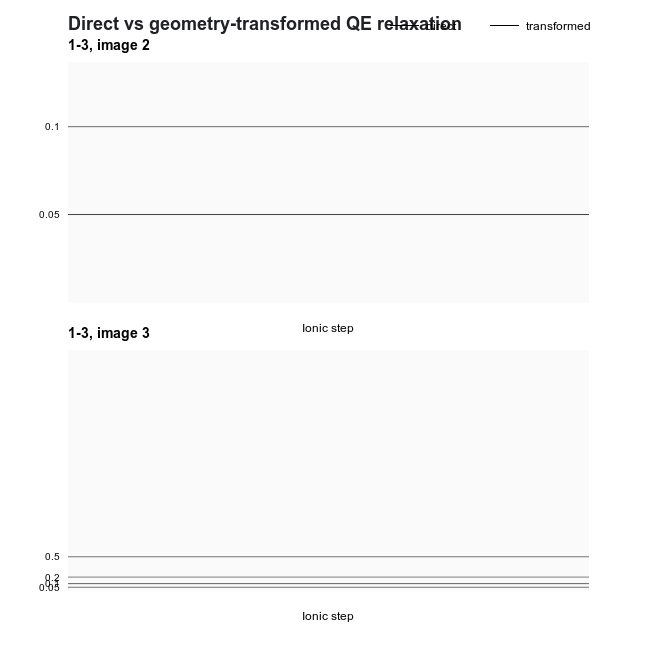
\includegraphics[width=\linewidth,height=0.42\textheight,keepaspectratio]{figure_pages/assets/fig_145.png}
\caption{Archived endpoint-relaxation or endpoint-quality evidence. This page shows the candidate output ``Force relaxation curves'' within the audited ARCHIVE-ENDPOINT family. The panel identity, source scope, and current status are retained in the accompanying evidence matrix.}
\label{fig:candidate_145}
\end{figure}
\textbf{Results text draft.} The figure preserves endpoint candidates and their quality flags as an auditable historical record. Endpoint stability is reported separately from path and transition-state validity.
\textbf{Discussion and boundary.} Use for provenance and candidate selection. Endpoints alone cannot validate a migration barrier or a complete NEB pathway.
\textbf{Article placement.} Proposed article location: SI endpoint-relaxation evidence.
\textbf{Reviewer linkage:} overall status NO\_DIRECT\_REVIEWER\_FIGURE\_LINK.
No direct reviewer-response figure linkage was identified; this page is retained for scientific/article audit rather than as a direct reviewer response.
\textbf{Evidence pointers.}
\begin{itemize}[leftmargin=1.4em,noitemsep]
\item Data/processed: \begingroup\scriptsize\url{paper/data/published/qe_geometry_transform_relax_ab_s47/comparison/1-3/paired_relaxation_comparison.csv}\endgroup
\item Data/processed: \begingroup\scriptsize\url{paper/data/published/qe_geometry_transform_relax_ab_s47/comparison/1-3/paired_relaxation_comparison.json}\endgroup
\item Caption/text source: \begingroup\scriptsize\url{paper/data/published/qe_geometry_transform_relax_ab_s47/comparison/1-3/README.md}\endgroup
\end{itemize}
\statusline{\textbf{Audit gap / next action:} Recover generator and exact raw log lineage}
\vfill
\clearpage
\section{FIG-146 --- Force relaxation curves}
\label{figpage:fig-146}
\textbf{Group:} ARCHIVE-ENDPOINT\quad \textbf{Evidence chain:} partial\quad \textbf{Status:} publication;comparison
\begin{figure}[H]
\centering
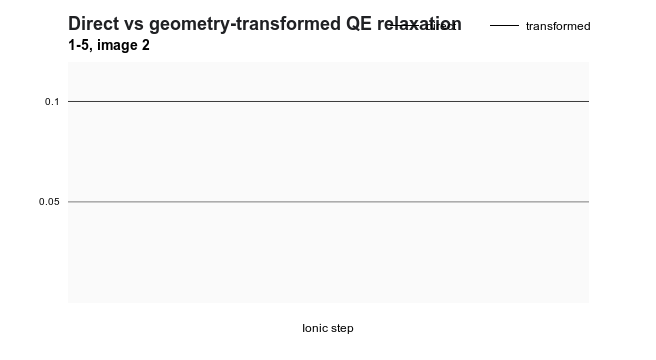
\includegraphics[width=\linewidth,height=0.42\textheight,keepaspectratio]{figure_pages/assets/fig_146.png}
\caption{Archived endpoint-relaxation or endpoint-quality evidence. This page shows the candidate output ``Force relaxation curves'' within the audited ARCHIVE-ENDPOINT family. The panel identity, source scope, and current status are retained in the accompanying evidence matrix.}
\label{fig:candidate_146}
\end{figure}
\textbf{Results text draft.} The figure preserves endpoint candidates and their quality flags as an auditable historical record. Endpoint stability is reported separately from path and transition-state validity.
\textbf{Discussion and boundary.} Use for provenance and candidate selection. Endpoints alone cannot validate a migration barrier or a complete NEB pathway.
\textbf{Article placement.} Proposed article location: SI endpoint-relaxation evidence.
\textbf{Reviewer linkage:} overall status NO\_DIRECT\_REVIEWER\_FIGURE\_LINK.
No direct reviewer-response figure linkage was identified; this page is retained for scientific/article audit rather than as a direct reviewer response.
\textbf{Evidence pointers.}
\begin{itemize}[leftmargin=1.4em,noitemsep]
\item Data/processed: \begingroup\scriptsize\url{paper/data/published/qe_geometry_transform_relax_ab_s47/comparison/1-5/paired_relaxation_comparison.csv}\endgroup
\item Data/processed: \begingroup\scriptsize\url{paper/data/published/qe_geometry_transform_relax_ab_s47/comparison/1-5/paired_relaxation_comparison.json}\endgroup
\item Caption/text source: \begingroup\scriptsize\url{paper/data/published/qe_geometry_transform_relax_ab_s47/comparison/1-5/README.md}\endgroup
\end{itemize}
\statusline{\textbf{Audit gap / next action:} Recover generator and exact raw log lineage}
\vfill
\clearpage
\section{FIG-147 --- Sb2te3cr 61 coverage}
\label{figpage:fig-147}
\textbf{Group:} ARCHIVE-TRAJ-PORTFOLIO\quad \textbf{Evidence chain:} partial\quad \textbf{Status:} publication
\begin{figure}[H]
\centering
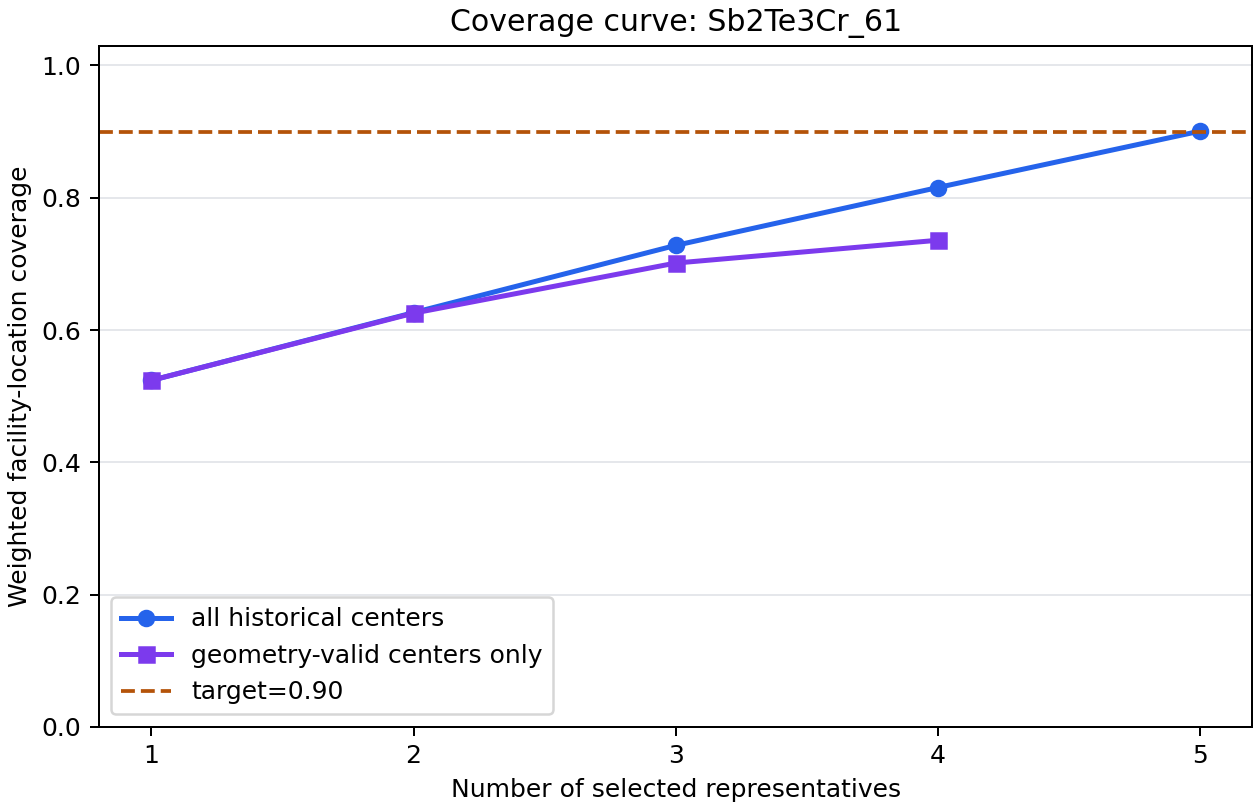
\includegraphics[width=\linewidth,height=0.42\textheight,keepaspectratio]{figure_pages/assets/fig_147.png}
\caption{Archived trajectory portfolio and model/protocol comparison. This page shows the candidate output ``Sb2te3cr 61 coverage'' within the audited ARCHIVE-TRAJ-PORTFOLIO family. The panel identity, source scope, and current status are retained in the accompanying evidence matrix.}
\label{fig:candidate_147}
\end{figure}
\textbf{Results text draft.} The figure assembles the available trajectory branches and their associated protocol or quality metadata. Different seeds, model families, and trajectory lengths remain separately identifiable.
\textbf{Discussion and boundary.} Use for coverage and provenance. Formal ranking requires the matched-protocol subset and accepted trajectory gates.
\textbf{Article placement.} Proposed article location: Methods/SI data coverage audit.
\textbf{Reviewer linkage:} overall status NO\_DIRECT\_REVIEWER\_FIGURE\_LINK.
No direct reviewer-response figure linkage was identified; this page is retained for scientific/article audit rather than as a direct reviewer response.
\textbf{Evidence pointers.}
\begin{itemize}[leftmargin=1.4em,noitemsep]
\item Data/processed: \begingroup\scriptsize\url{paper/data/published/representative_trajectory_portfolio/coverage_gaps.csv}\endgroup
\item Data/processed: \begingroup\scriptsize\url{paper/data/published/representative_trajectory_portfolio/pairwise_trajectory_distances.csv}\endgroup
\end{itemize}
\statusline{\textbf{Audit gap / next action:} Figure generator is not co-located with the archived image}
\vfill
\clearpage
\section{FIG-148 --- Sb2te3cr 61 similarity}
\label{figpage:fig-148}
\textbf{Group:} ARCHIVE-TRAJ-PORTFOLIO\quad \textbf{Evidence chain:} partial\quad \textbf{Status:} publication
\begin{figure}[H]
\centering
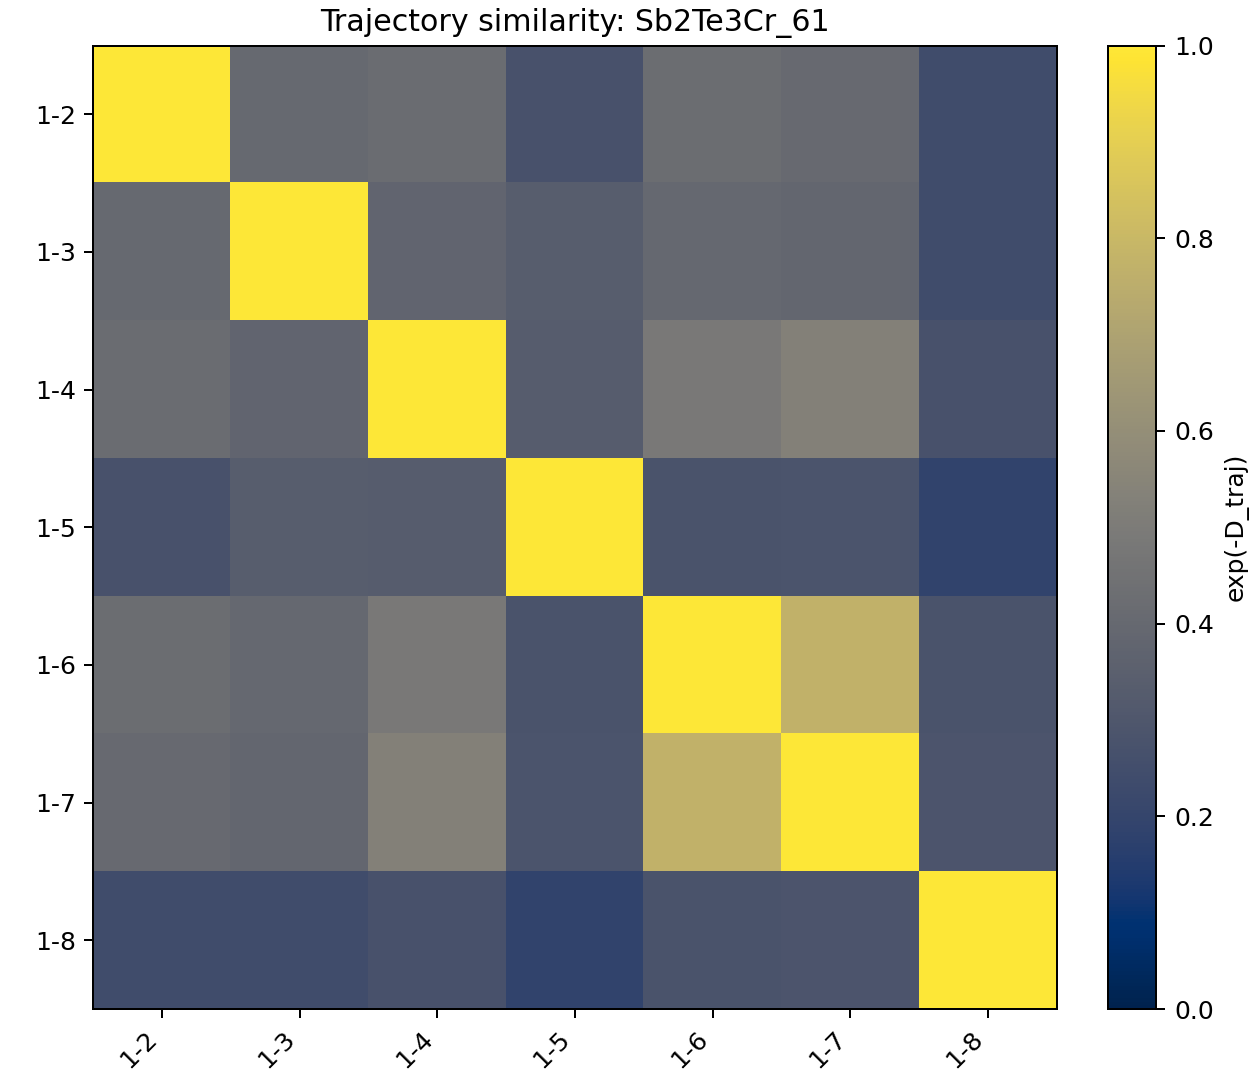
\includegraphics[width=\linewidth,height=0.42\textheight,keepaspectratio]{figure_pages/assets/fig_148.png}
\caption{Archived trajectory portfolio and model/protocol comparison. This page shows the candidate output ``Sb2te3cr 61 similarity'' within the audited ARCHIVE-TRAJ-PORTFOLIO family. The panel identity, source scope, and current status are retained in the accompanying evidence matrix.}
\label{fig:candidate_148}
\end{figure}
\textbf{Results text draft.} The figure assembles the available trajectory branches and their associated protocol or quality metadata. Different seeds, model families, and trajectory lengths remain separately identifiable.
\textbf{Discussion and boundary.} Use for coverage and provenance. Formal ranking requires the matched-protocol subset and accepted trajectory gates.
\textbf{Article placement.} Proposed article location: Methods/SI data coverage audit.
\textbf{Reviewer linkage:} overall status NO\_DIRECT\_REVIEWER\_FIGURE\_LINK.
No direct reviewer-response figure linkage was identified; this page is retained for scientific/article audit rather than as a direct reviewer response.
\textbf{Evidence pointers.}
\begin{itemize}[leftmargin=1.4em,noitemsep]
\item Data/processed: \begingroup\scriptsize\url{paper/data/published/representative_trajectory_portfolio/coverage_gaps.csv}\endgroup
\item Data/processed: \begingroup\scriptsize\url{paper/data/published/representative_trajectory_portfolio/pairwise_trajectory_distances.csv}\endgroup
\end{itemize}
\statusline{\textbf{Audit gap / next action:} Figure generator is not co-located with the archived image}
\vfill
\clearpage
\section{FIG-149 --- Sb2te3cr 81 coverage}
\label{figpage:fig-149}
\textbf{Group:} ARCHIVE-TRAJ-PORTFOLIO\quad \textbf{Evidence chain:} partial\quad \textbf{Status:} publication
\begin{figure}[H]
\centering
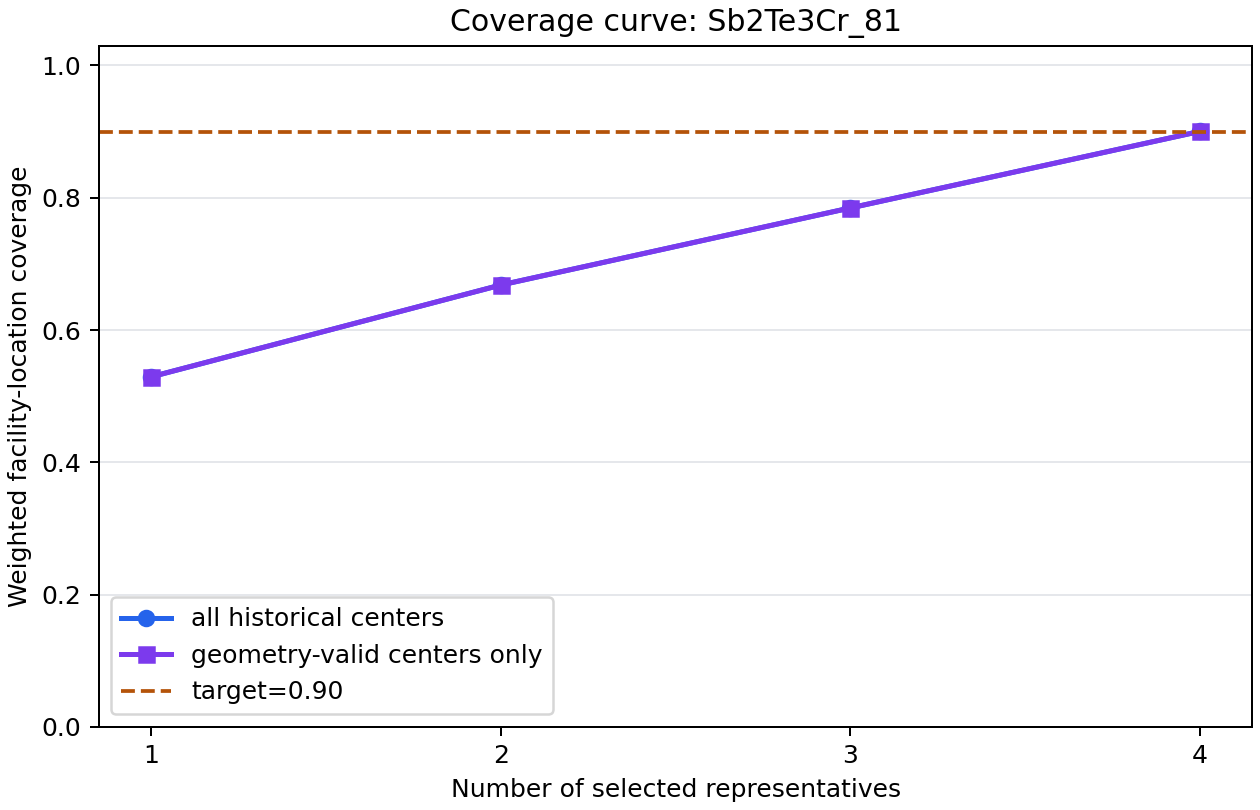
\includegraphics[width=\linewidth,height=0.42\textheight,keepaspectratio]{figure_pages/assets/fig_149.png}
\caption{Archived trajectory portfolio and model/protocol comparison. This page shows the candidate output ``Sb2te3cr 81 coverage'' within the audited ARCHIVE-TRAJ-PORTFOLIO family. The panel identity, source scope, and current status are retained in the accompanying evidence matrix.}
\label{fig:candidate_149}
\end{figure}
\textbf{Results text draft.} The figure assembles the available trajectory branches and their associated protocol or quality metadata. Different seeds, model families, and trajectory lengths remain separately identifiable.
\textbf{Discussion and boundary.} Use for coverage and provenance. Formal ranking requires the matched-protocol subset and accepted trajectory gates.
\textbf{Article placement.} Proposed article location: Methods/SI data coverage audit.
\textbf{Reviewer linkage:} overall status NO\_DIRECT\_REVIEWER\_FIGURE\_LINK.
No direct reviewer-response figure linkage was identified; this page is retained for scientific/article audit rather than as a direct reviewer response.
\textbf{Evidence pointers.}
\begin{itemize}[leftmargin=1.4em,noitemsep]
\item Data/processed: \begingroup\scriptsize\url{paper/data/published/representative_trajectory_portfolio/coverage_gaps.csv}\endgroup
\item Data/processed: \begingroup\scriptsize\url{paper/data/published/representative_trajectory_portfolio/pairwise_trajectory_distances.csv}\endgroup
\end{itemize}
\statusline{\textbf{Audit gap / next action:} Figure generator is not co-located with the archived image}
\vfill
\clearpage
\section{FIG-150 --- Sb2te3cr 81 similarity}
\label{figpage:fig-150}
\textbf{Group:} ARCHIVE-TRAJ-PORTFOLIO\quad \textbf{Evidence chain:} partial\quad \textbf{Status:} publication
\begin{figure}[H]
\centering
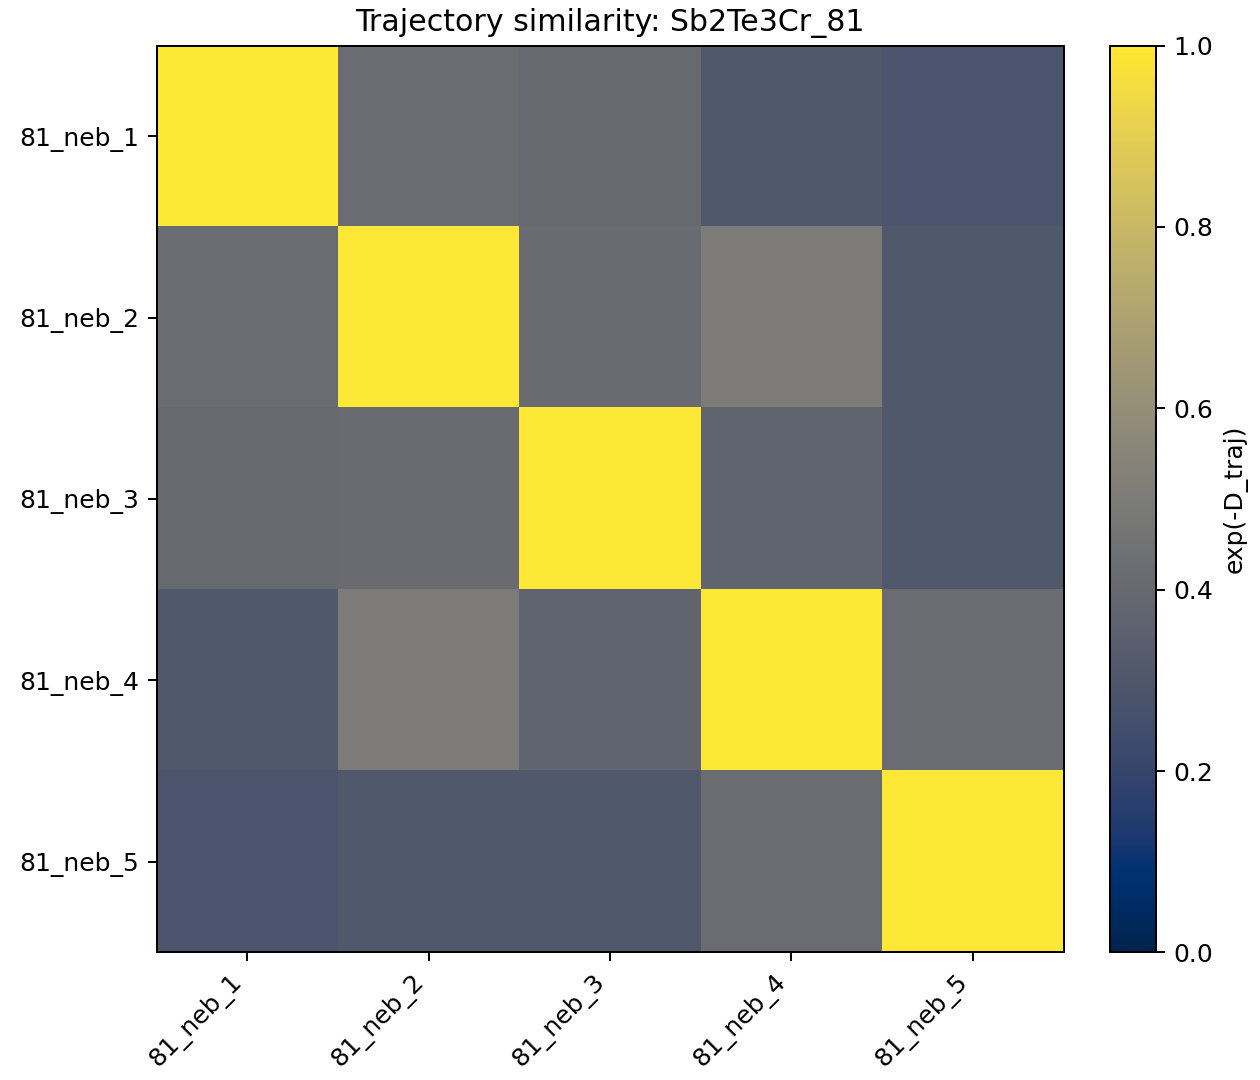
\includegraphics[width=\linewidth,height=0.42\textheight,keepaspectratio]{figure_pages/assets/fig_150.png}
\caption{Archived trajectory portfolio and model/protocol comparison. This page shows the candidate output ``Sb2te3cr 81 similarity'' within the audited ARCHIVE-TRAJ-PORTFOLIO family. The panel identity, source scope, and current status are retained in the accompanying evidence matrix.}
\label{fig:candidate_150}
\end{figure}
\textbf{Results text draft.} The figure assembles the available trajectory branches and their associated protocol or quality metadata. Different seeds, model families, and trajectory lengths remain separately identifiable.
\textbf{Discussion and boundary.} Use for coverage and provenance. Formal ranking requires the matched-protocol subset and accepted trajectory gates.
\textbf{Article placement.} Proposed article location: Methods/SI data coverage audit.
\textbf{Reviewer linkage:} overall status NO\_DIRECT\_REVIEWER\_FIGURE\_LINK.
No direct reviewer-response figure linkage was identified; this page is retained for scientific/article audit rather than as a direct reviewer response.
\textbf{Evidence pointers.}
\begin{itemize}[leftmargin=1.4em,noitemsep]
\item Data/processed: \begingroup\scriptsize\url{paper/data/published/representative_trajectory_portfolio/coverage_gaps.csv}\endgroup
\item Data/processed: \begingroup\scriptsize\url{paper/data/published/representative_trajectory_portfolio/pairwise_trajectory_distances.csv}\endgroup
\end{itemize}
\statusline{\textbf{Audit gap / next action:} Figure generator is not co-located with the archived image}
\vfill
\clearpage
\section{FIG-151 --- Leakage distance distributions}
\label{figpage:fig-151}
\textbf{Group:} ARCHIVE-LEAKAGE\quad \textbf{Evidence chain:} partial\quad \textbf{Status:} publication;audit
\begin{figure}[H]
\centering
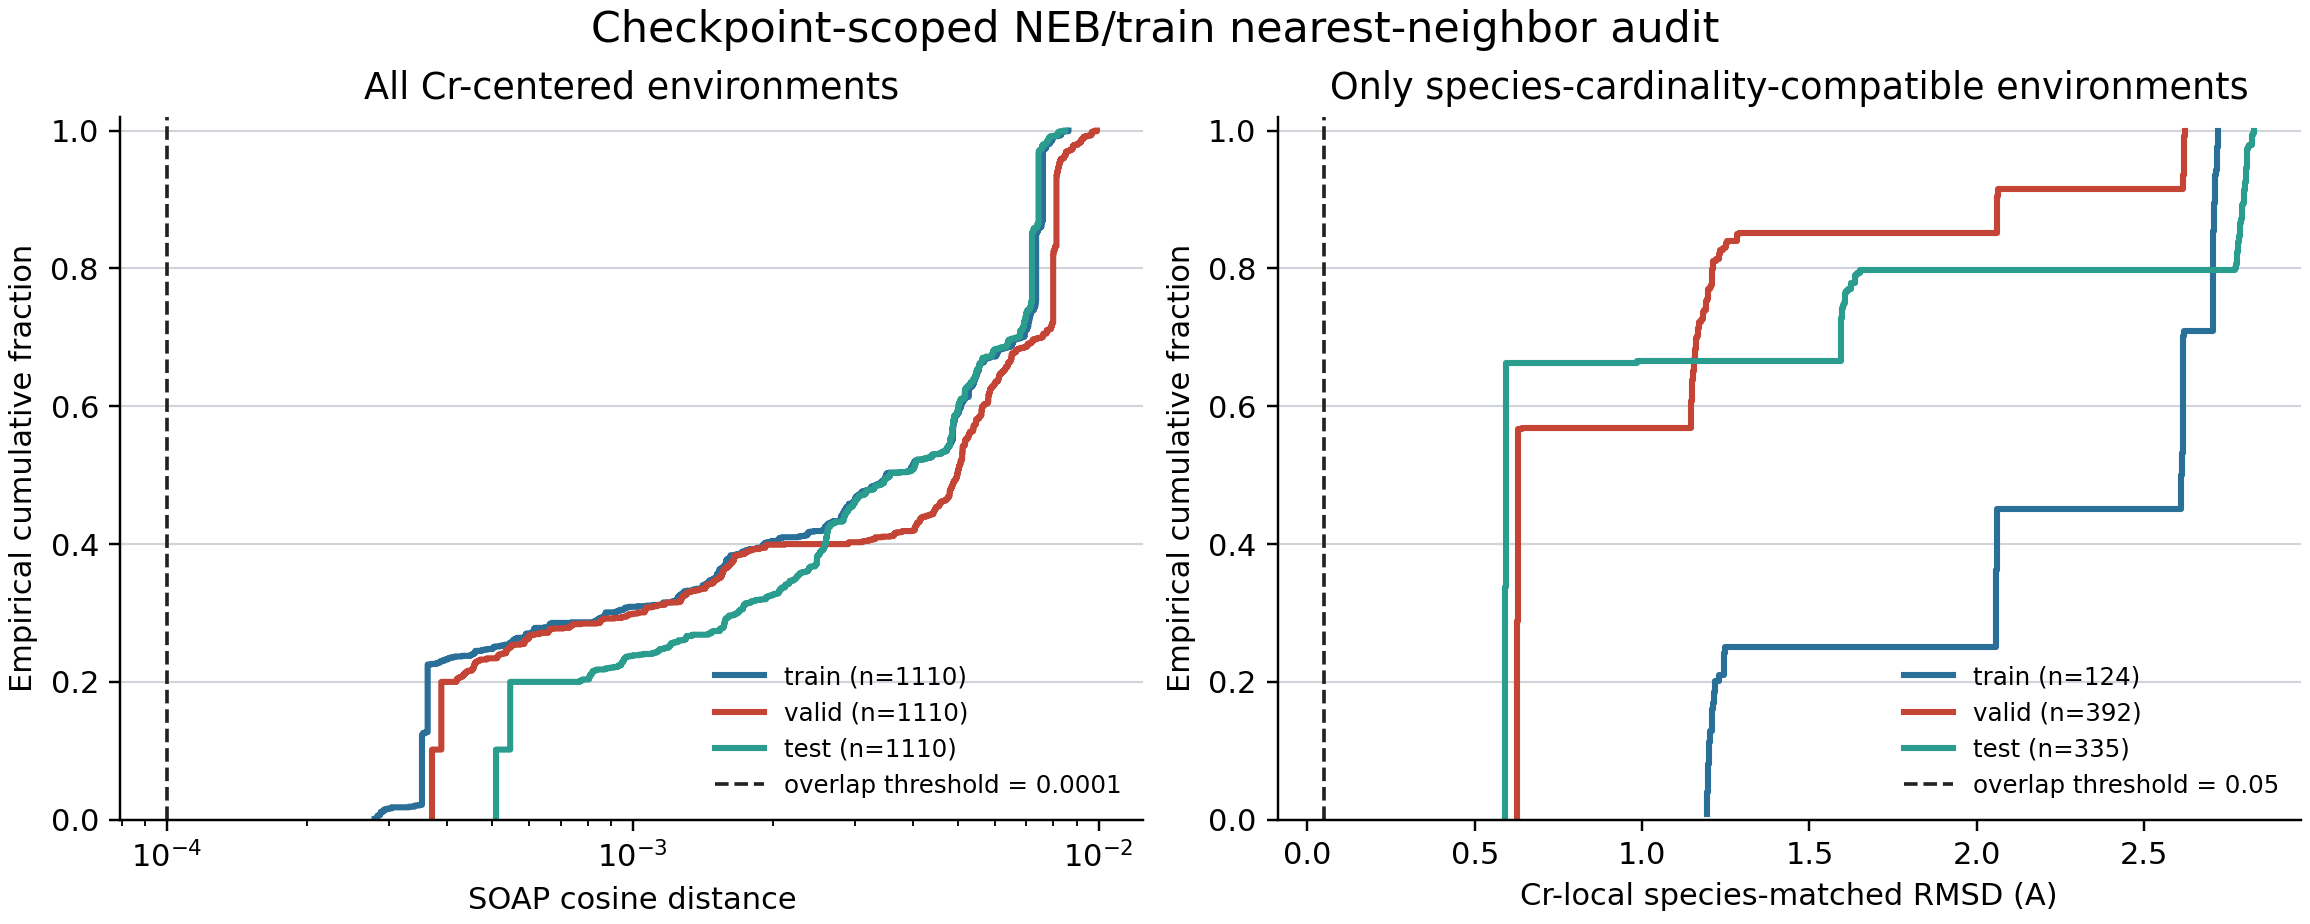
\includegraphics[width=\linewidth,height=0.42\textheight,keepaspectratio]{figure_pages/assets/fig_151.png}
\caption{Archived training/test proximity or leakage audit. This page shows the candidate output ``Leakage distance distributions'' within the audited ARCHIVE-LEAKAGE family. The panel identity, source scope, and current status are retained in the accompanying evidence matrix.}
\label{fig:candidate_151}
\end{figure}
\textbf{Results text draft.} The figure shows the available proximity or leakage diagnostics under the declared representation and threshold. The source scope is part of the result and must remain visible.
\textbf{Discussion and boundary.} This supports a data-separation claim only for the audited scope; it does not generalize to model families or datasets that were not included in the audit.
\textbf{Article placement.} Proposed article location: Methods/Results data provenance.
\textbf{Reviewer linkage:} overall status DONE.
\begin{itemize}[leftmargin=1.4em,noitemsep]
\item \textbf{REV-A2 (DONE):} Rule out train/test overlap between in-gap NEB images and FT-600K training frames. \emph{Completed:} Grouped splitting and the SOAP/RMSD nearest-neighbor audit are complete for the declared training scopes; the historical 0.16 eV point is not silently reused. \emph{Still required:} No additional figure evidence is required for the completed scope; retain the thresholds, source scope, and manifest in the final release.
\item \textbf{REV-C10 (DONE):} Replace the frame-level random split with a grouped train/test split and overlap audit. \emph{Completed:} Grouped-split retraining, zero-overlap checks, and the revised RMSE/barrier statistics are available for the declared models and seeds. \emph{Still required:} Keep historical frame-level values visibly labeled and use grouped values for generalization claims.
\end{itemize}
\textbf{Evidence pointers.}
\begin{itemize}[leftmargin=1.4em,noitemsep]
\item Data/processed: \begingroup\scriptsize\url{paper/data/published/training_leakage_audit/checkpoint_finetuned_MACE_multihead0804_s42/leakage_audit.json}\endgroup
\item Data/processed: \begingroup\scriptsize\url{paper/data/published/training_leakage_audit/checkpoint_finetuned_MACE_multihead0804_s42/leakage_distance_summary.csv}\endgroup
\end{itemize}
\statusline{\textbf{Audit gap / next action:} Generator is outside the figure directory; link exact source script}
\vfill
\clearpage
\section{FIG-152 --- Fig6 shap revised}
\label{figpage:fig-152}
\textbf{Group:} LEGACY-PUBLISHED\quad \textbf{Evidence chain:} partial\quad \textbf{Status:} publication
\begin{figure}[H]
\centering
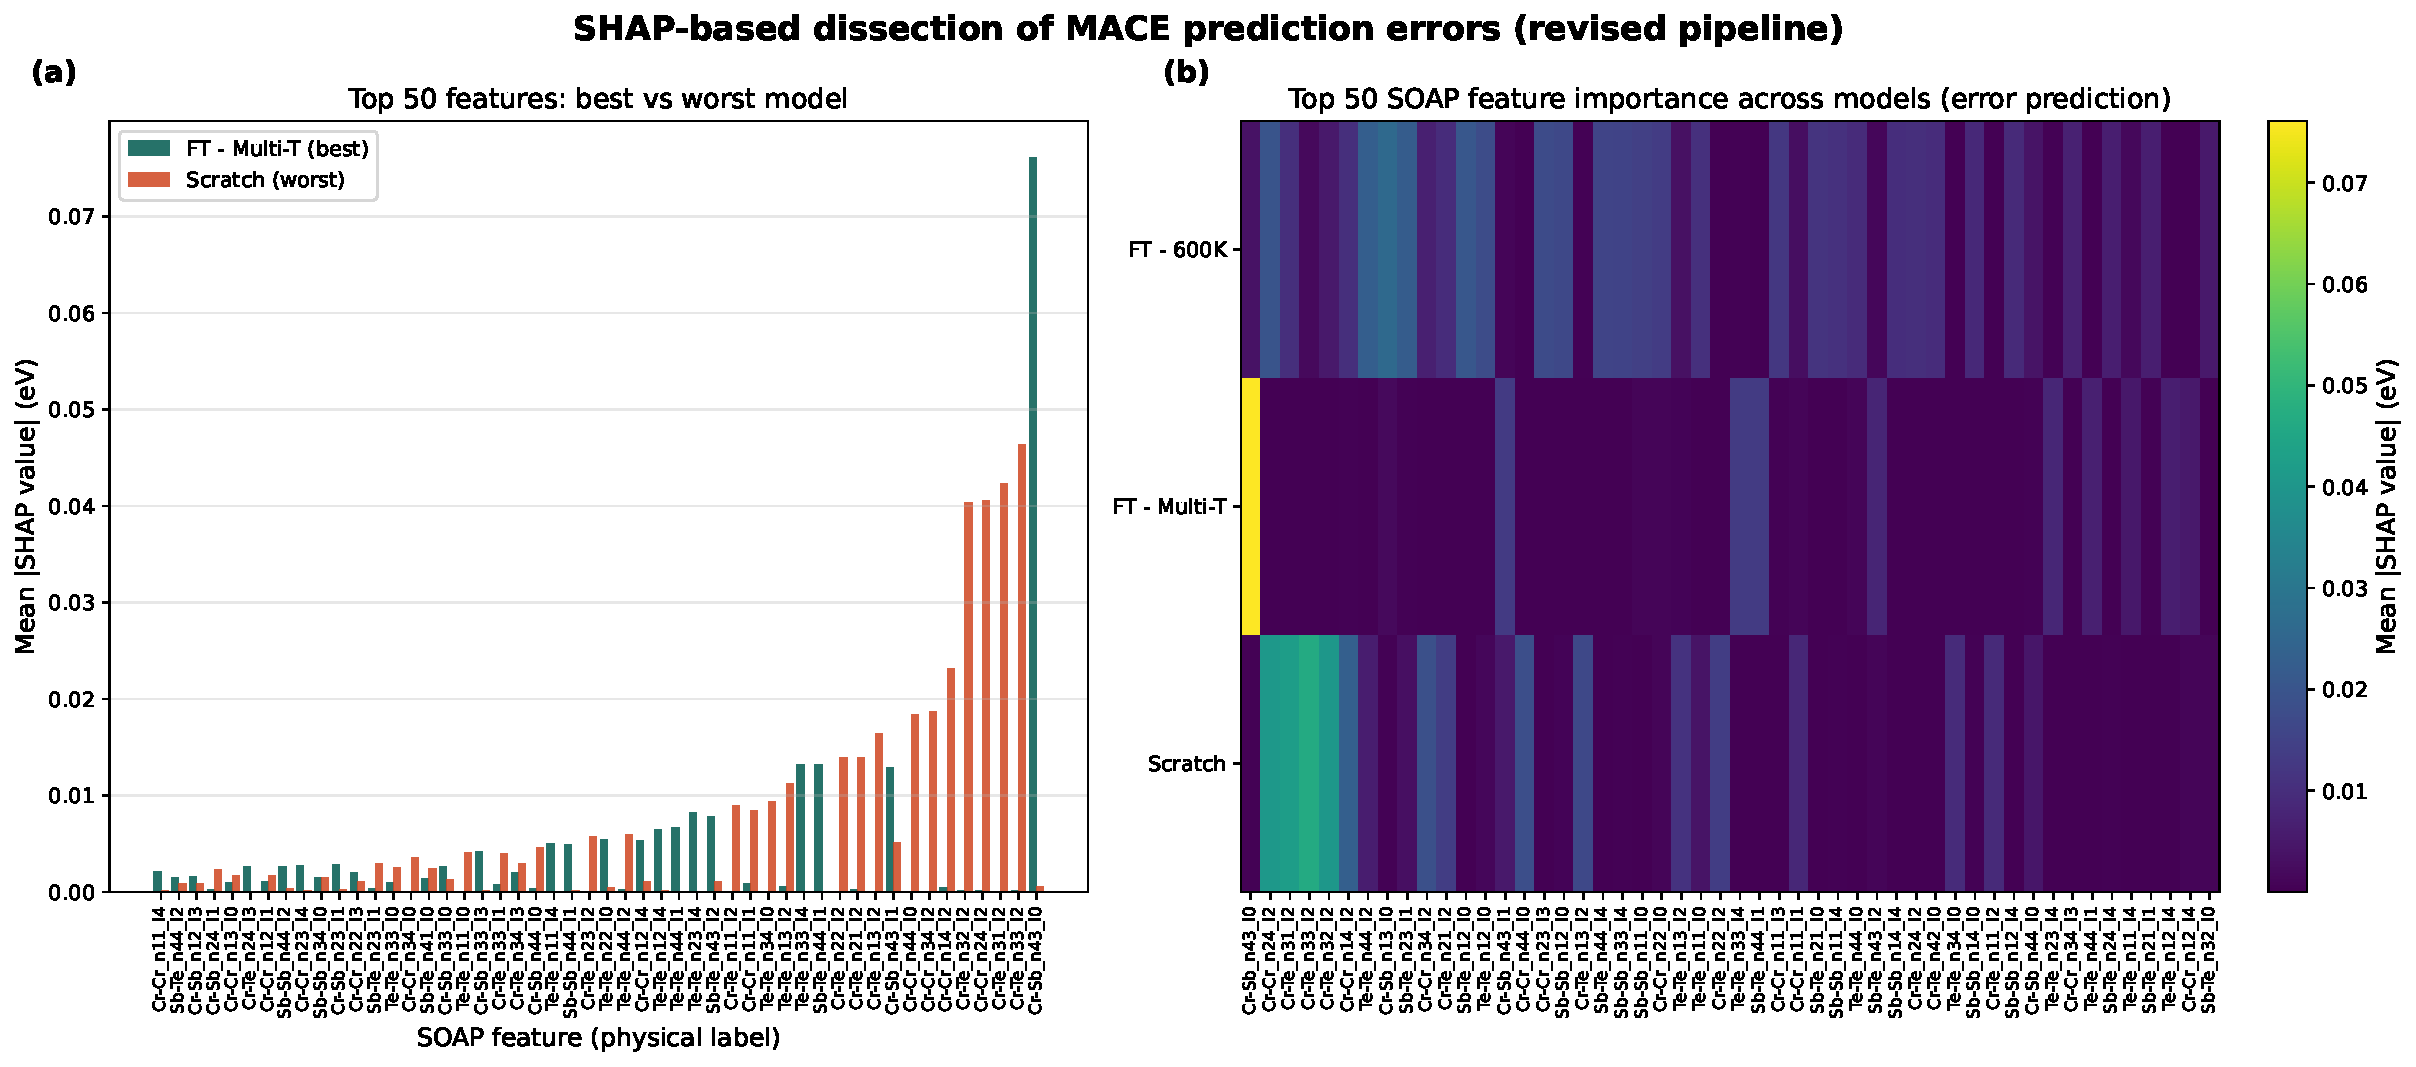
\includegraphics[width=\linewidth,height=0.42\textheight,keepaspectratio]{figure_pages/assets/fig_152.pdf}
\caption{Legacy published figure retained for source and manuscript reconciliation. This page shows the candidate output ``Fig6 shap revised'' within the audited LEGACY-PUBLISHED family. The panel identity, source scope, and current status are retained in the accompanying evidence matrix.}
\label{fig:candidate_152}
\end{figure}
\textbf{Results text draft.} This page preserves the previously published visualization while linking it to the current source ledger and revision status.
\textbf{Discussion and boundary.} The figure should be replaced or relabeled if the current audit changes the underlying data scope, protocol, or interpretation.
\textbf{Article placement.} Proposed article location: Revision1 manuscript asset.
\textbf{Reviewer linkage:} overall status PARTIAL.
\begin{itemize}[leftmargin=1.4em,noitemsep]
\item \textbf{REV-A6 (PARTIAL):} Soften t-SNE/PHATE and SHAP interpretation claims and add projection/original-space and surrogate-fidelity checks. \emph{Completed:} Projection sensitivity, original-descriptor-space separation, and per-model cross-validated surrogate R2 are available; the text is scoped to descriptive/surrogate evidence. \emph{Still required:} A direct MACE Cr-Cr perturbation test remains pending if a causal claim about the dominant feature is desired; otherwise retain the surrogate-scoped wording.
\item \textbf{REV-C13 (PARTIAL):} Make the SHAP pipeline and advertised repository artifacts reproducible rather than leaving empty stubs. \emph{Completed:} The corrected SHAP inputs, scripts, lineage, and locked revised outputs are present for the declared three-model/150-frame scope. \emph{Still required:} Close the final release/empty-stub audit and reconcile the independent rerun with the locked historical CSV before claiming exact end-to-end regeneration.
\end{itemize}
\textbf{Evidence pointers.}
No data/script/text candidate was recorded in the matrix; resolve this gap before manuscript promotion.
\statusline{\textbf{Audit gap / next action:} Link to canonical revision1 asset and generator}
\vfill
\clearpage
\section{FIG-153 --- Figs dft neb mep profiles}
\label{figpage:fig-153}
\textbf{Group:} LEGACY-PUBLISHED\quad \textbf{Evidence chain:} partial\quad \textbf{Status:} publication;comparison
\begin{figure}[H]
\centering
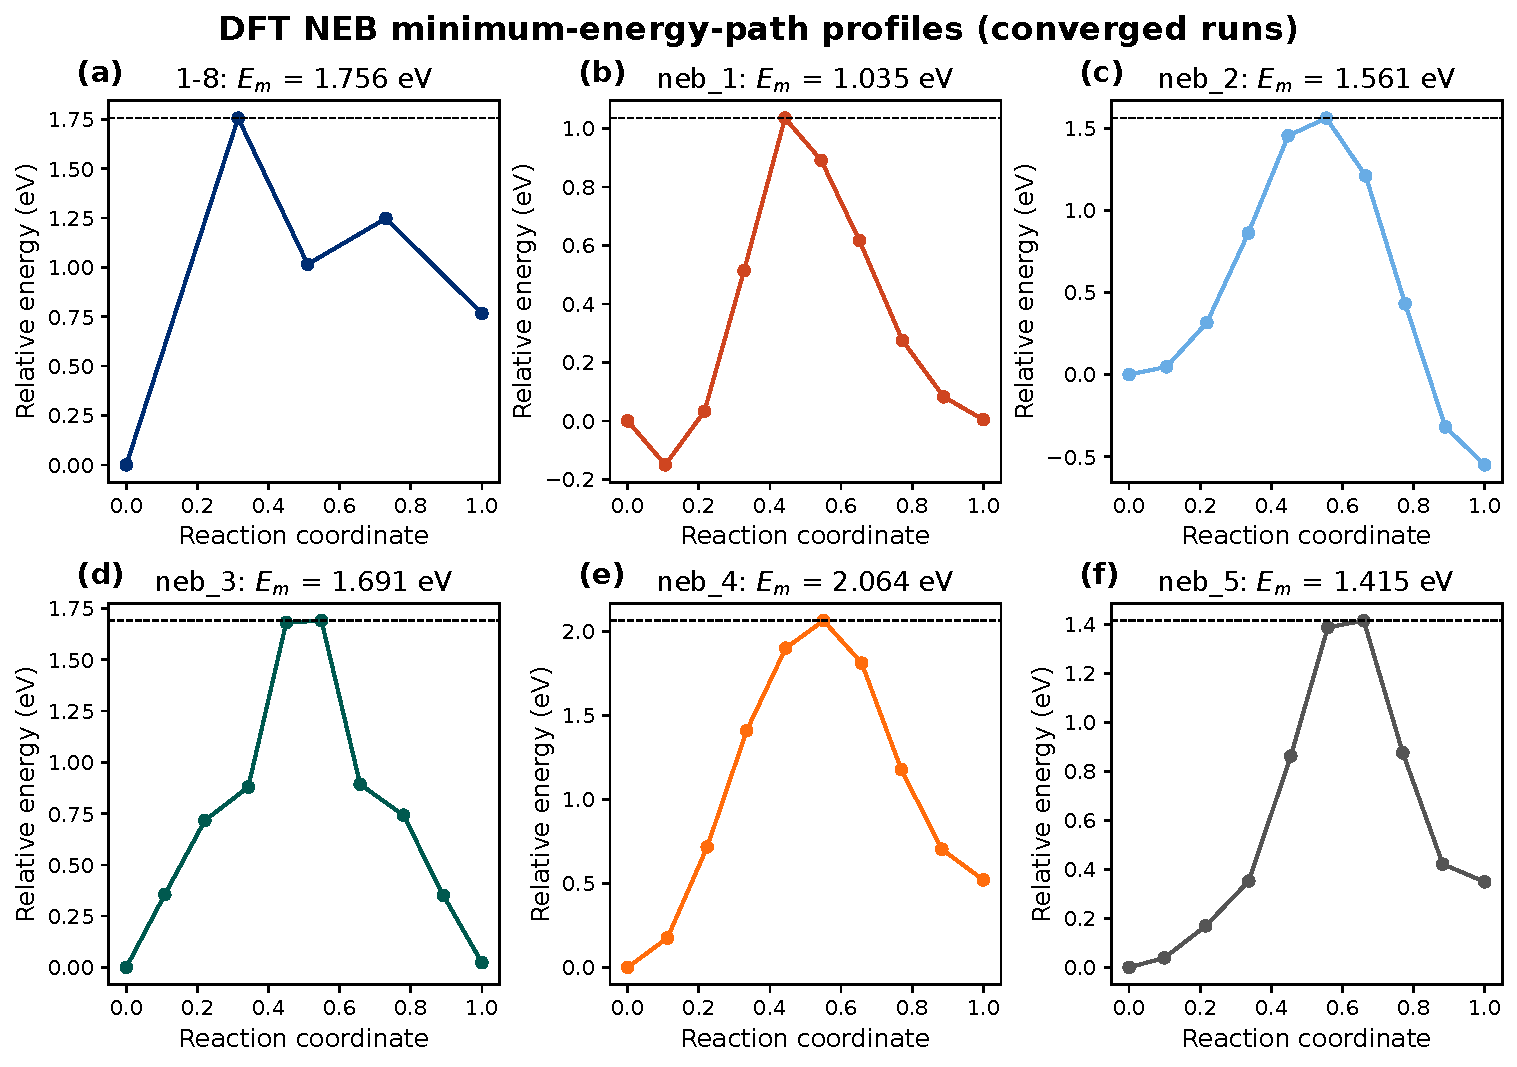
\includegraphics[width=\linewidth,height=0.42\textheight,keepaspectratio]{figure_pages/assets/fig_153.pdf}
\caption{Legacy published figure retained for source and manuscript reconciliation. This page shows the candidate output ``Figs dft neb mep profiles'' within the audited LEGACY-PUBLISHED family. The panel identity, source scope, and current status are retained in the accompanying evidence matrix.}
\label{fig:candidate_153}
\end{figure}
\textbf{Results text draft.} This page preserves the previously published visualization while linking it to the current source ledger and revision status.
\textbf{Discussion and boundary.} The figure should be replaced or relabeled if the current audit changes the underlying data scope, protocol, or interpretation.
\textbf{Article placement.} Proposed article location: Revision1 manuscript asset.
\textbf{Reviewer linkage:} overall status PARTIAL.
\begin{itemize}[leftmargin=1.4em,noitemsep]
\item \textbf{REV-A1 (PARTIAL):} Reconcile Fig. 3d fixed-geometry DFT-path scoring with SI Fig. S3 self-consistent MLFF-NEB, including pathway identity and the DFT reference. \emph{Completed:} The fixed-path versus self-relaxed operator distinction and the narrower model-reported-barrier wording are integrated. \emph{Still required:} Close the restartable QE path-1--4 convergence gate, preserve the final path/source metadata, and complete the SI Fig. S3 endpoint/checkpoint/optimizer/source audit before calling the quantitative reference final.
\end{itemize}
\textbf{Evidence pointers.}
No data/script/text candidate was recorded in the matrix; resolve this gap before manuscript promotion.
\statusline{\textbf{Audit gap / next action:} Link to canonical revision1 asset and generator}
\vfill
\clearpage
\section{FIG-154 --- Figs latent robustness}
\label{figpage:fig-154}
\textbf{Group:} LEGACY-PUBLISHED\quad \textbf{Evidence chain:} partial\quad \textbf{Status:} publication
\begin{figure}[H]
\centering
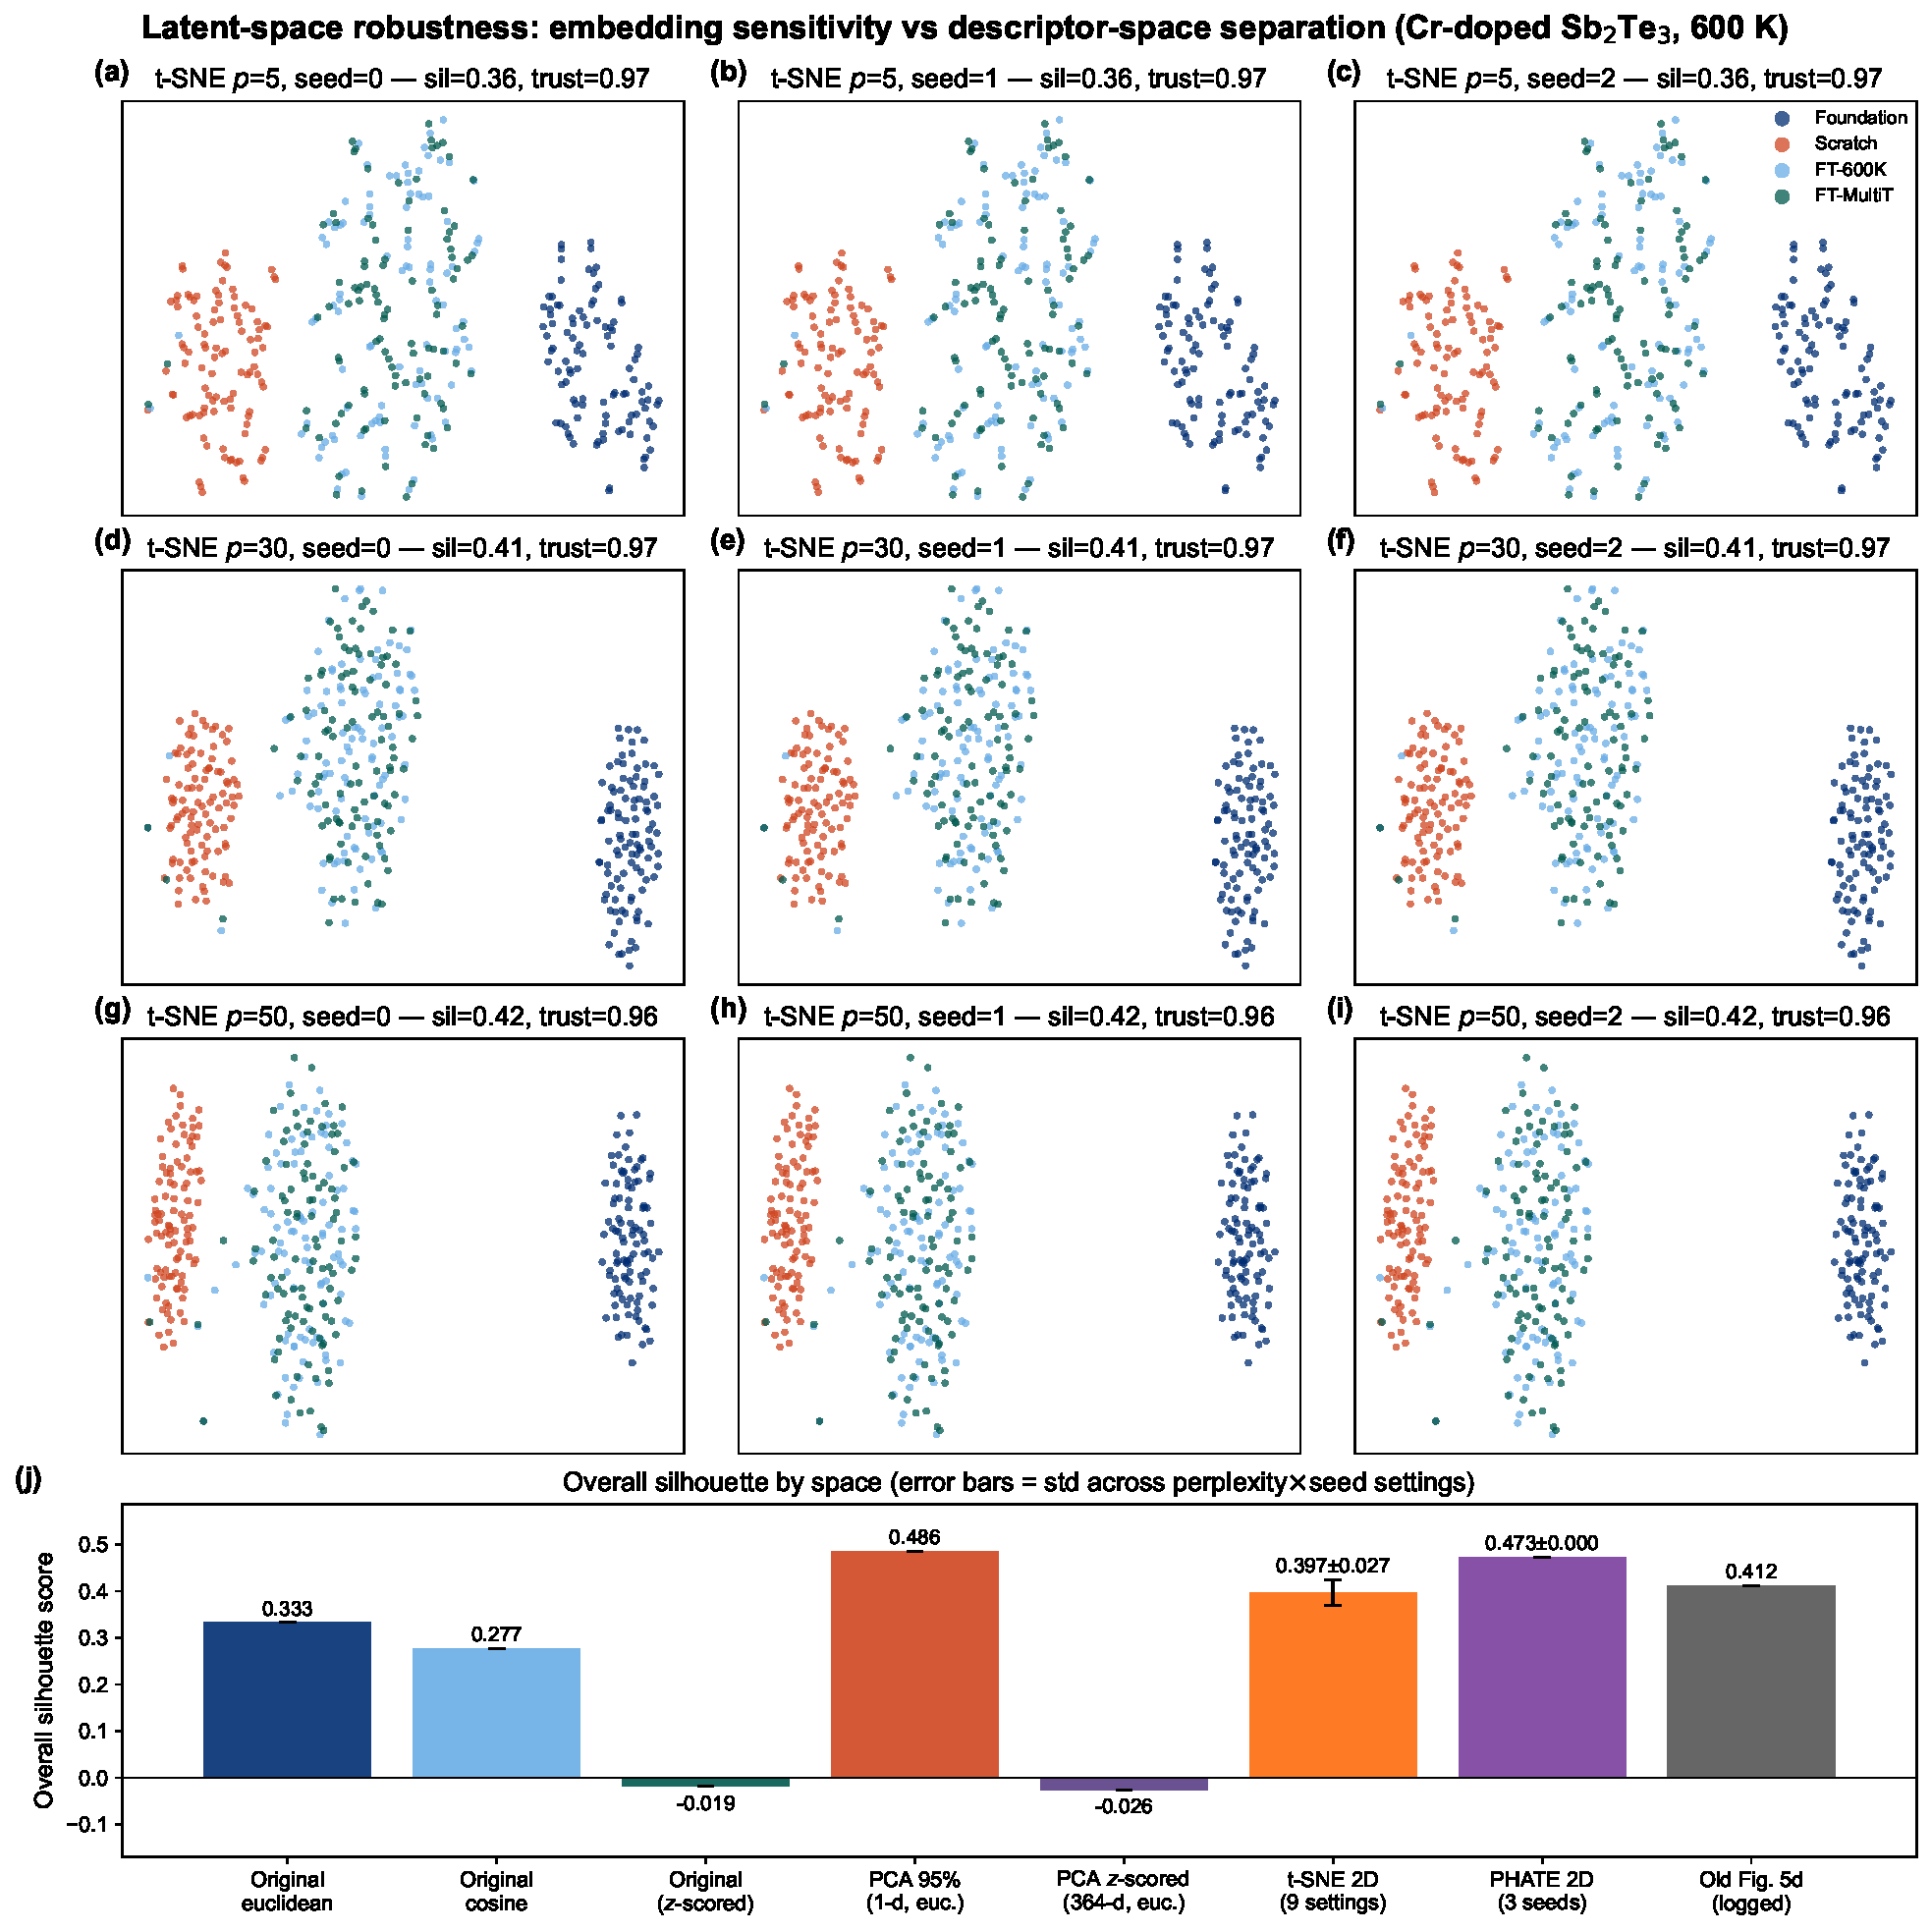
\includegraphics[width=\linewidth,height=0.42\textheight,keepaspectratio]{figure_pages/assets/fig_154.pdf}
\caption{Legacy published figure retained for source and manuscript reconciliation. This page shows the candidate output ``Figs latent robustness'' within the audited LEGACY-PUBLISHED family. The panel identity, source scope, and current status are retained in the accompanying evidence matrix.}
\label{fig:candidate_154}
\end{figure}
\textbf{Results text draft.} This page preserves the previously published visualization while linking it to the current source ledger and revision status.
\textbf{Discussion and boundary.} The figure should be replaced or relabeled if the current audit changes the underlying data scope, protocol, or interpretation.
\textbf{Article placement.} Proposed article location: Revision1 manuscript asset.
\textbf{Reviewer linkage:} overall status PARTIAL.
\begin{itemize}[leftmargin=1.4em,noitemsep]
\item \textbf{REV-A6 (PARTIAL):} Soften t-SNE/PHATE and SHAP interpretation claims and add projection/original-space and surrogate-fidelity checks. \emph{Completed:} Projection sensitivity, original-descriptor-space separation, and per-model cross-validated surrogate R2 are available; the text is scoped to descriptive/surrogate evidence. \emph{Still required:} A direct MACE Cr-Cr perturbation test remains pending if a causal claim about the dominant feature is desired; otherwise retain the surrogate-scoped wording.
\item \textbf{REV-C11 (DONE):} Compute separability in the original/high-dimensional descriptor space rather than only on a 2D embedding. \emph{Completed:} Original-space metrics and projection-sensitivity checks are available; embedding scores are retained only as descriptive baselines. \emph{Still required:} No new numerical figure is required; preserve the feature-space definition and scaling sensitivity in the caption/methods.
\item \textbf{REV-C12 (DONE):} Remove the always-zero force-sensitivity feature stub from the latent analysis. \emph{Completed:} The inactive channel was removed and no unsupported force-sensitivity claim is made. \emph{Still required:} No additional figure evidence is required unless a genuine finite-difference force-sensitivity analysis is later added.
\end{itemize}
\textbf{Evidence pointers.}
No data/script/text candidate was recorded in the matrix; resolve this gap before manuscript promotion.
\statusline{\textbf{Audit gap / next action:} Link to canonical revision1 asset and generator}
\vfill
\clearpage
\section{FIG-155 --- Figs neb pes local audit}
\label{figpage:fig-155}
\textbf{Group:} LEGACY-PUBLISHED\quad \textbf{Evidence chain:} partial\quad \textbf{Status:} publication;audit
\begin{figure}[H]
\centering
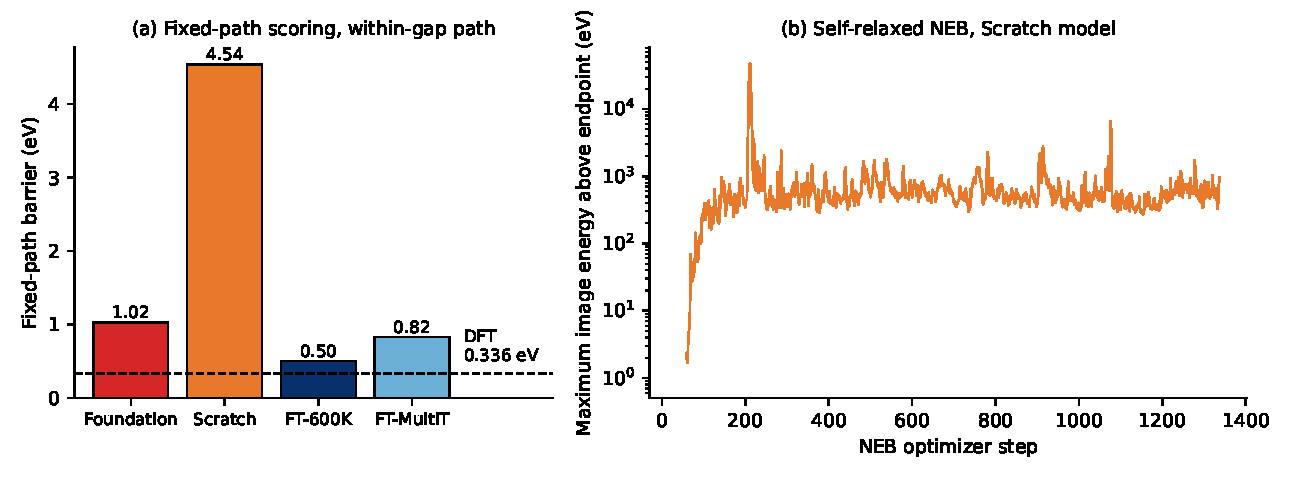
\includegraphics[width=\linewidth,height=0.42\textheight,keepaspectratio]{figure_pages/assets/fig_155_reader.pdf}
\caption{Legacy published figure retained for source and manuscript reconciliation. This page shows the candidate output ``Figs neb pes local audit'' within the audited LEGACY-PUBLISHED family. The panel identity, source scope, and current status are retained in the accompanying evidence matrix.}
\label{fig:candidate_155}
\end{figure}
\textbf{Results text draft.} This page preserves the previously published visualization while linking it to the current source ledger and revision status.
\textbf{Discussion and boundary.} The figure should be replaced or relabeled if the current audit changes the underlying data scope, protocol, or interpretation.
\textbf{Article placement.} Proposed article location: Revision1 manuscript asset.
\textbf{Reviewer linkage:} overall status PARTIAL.
\begin{itemize}[leftmargin=1.4em,noitemsep]
\item \textbf{REV-A1 (PARTIAL):} Reconcile Fig. 3d fixed-geometry DFT-path scoring with SI Fig. S3 self-consistent MLFF-NEB, including pathway identity and the DFT reference. \emph{Completed:} The fixed-path versus self-relaxed operator distinction and the narrower model-reported-barrier wording are integrated. \emph{Still required:} Close the restartable QE path-1--4 convergence gate, preserve the final path/source metadata, and complete the SI Fig. S3 endpoint/checkpoint/optimizer/source audit before calling the quantitative reference final.
\end{itemize}
\textbf{Evidence pointers.}
No data/script/text candidate was recorded in the matrix; resolve this gap before manuscript promotion.
\statusline{\textbf{Audit gap / next action:} Link to canonical revision1 asset and generator}
\vfill
\clearpage
\section{FIG-156 --- Fig md msd kappa revised}
\label{figpage:fig-156}
\textbf{Group:} LEGACY-PUBLISHED\quad \textbf{Evidence chain:} partial\quad \textbf{Status:} publication
\begin{figure}[H]
\centering
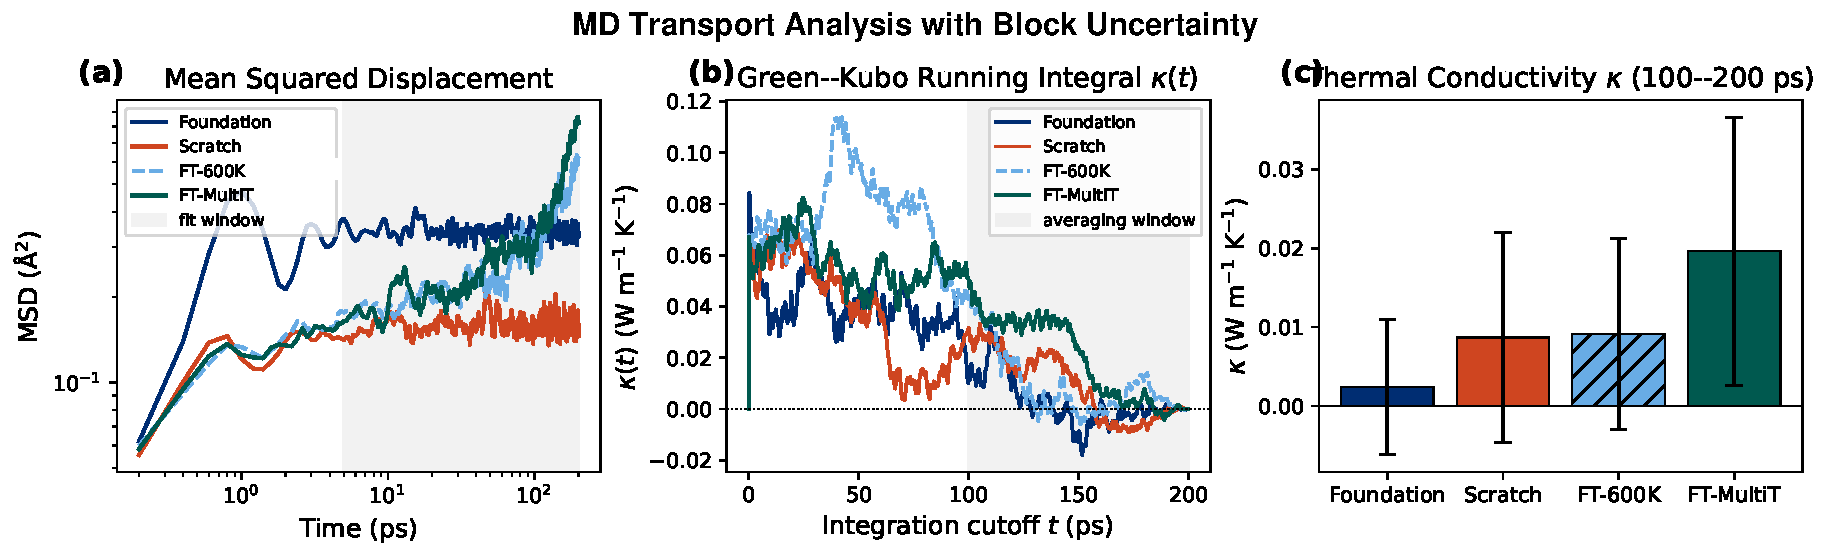
\includegraphics[width=\linewidth,height=0.42\textheight,keepaspectratio]{figure_pages/assets/fig_156_reader.pdf}
\caption{Legacy published figure retained for source and manuscript reconciliation. This page shows the candidate output ``Fig md msd kappa revised'' within the audited LEGACY-PUBLISHED family. The panel identity, source scope, and current status are retained in the accompanying evidence matrix.}
\label{fig:candidate_156}
\end{figure}
\textbf{Results text draft.} This page preserves the previously published visualization while linking it to the current source ledger and revision status.
\textbf{Discussion and boundary.} The figure should be replaced or relabeled if the current audit changes the underlying data scope, protocol, or interpretation.
\textbf{Article placement.} Proposed article location: Revision1 manuscript asset.
\textbf{Reviewer linkage:} overall status PENDING.
\begin{itemize}[leftmargin=1.4em,noitemsep]
\item \textbf{REV-C9 (PENDING):} Resolve the asymmetric FT-600K MD transport protocol and its effect on D and kappa. \emph{Completed:} Legacy FT-600K transport values are quarantined and excluded from ranking; the figure can document that boundary. \emph{Still required:} Run the corrected matched-protocol FT-600K long trajectory, block-average D/kappa, and close the multi-seed uncertainty before reporting a final transport comparison.
\end{itemize}
\textbf{Evidence pointers.}
No data/script/text candidate was recorded in the matrix; resolve this gap before manuscript promotion.
\statusline{\textbf{Audit gap / next action:} Link to canonical revision1 asset and generator}
\vfill
\clearpage
\section{FIG-157 --- Neurips2025 ai4mat em 1013}
\label{figpage:fig-157}
\textbf{Group:} LEGACY-NEURIPS\quad \textbf{Evidence chain:} partial\quad \textbf{Status:} publication
\begin{figure}[H]
\centering
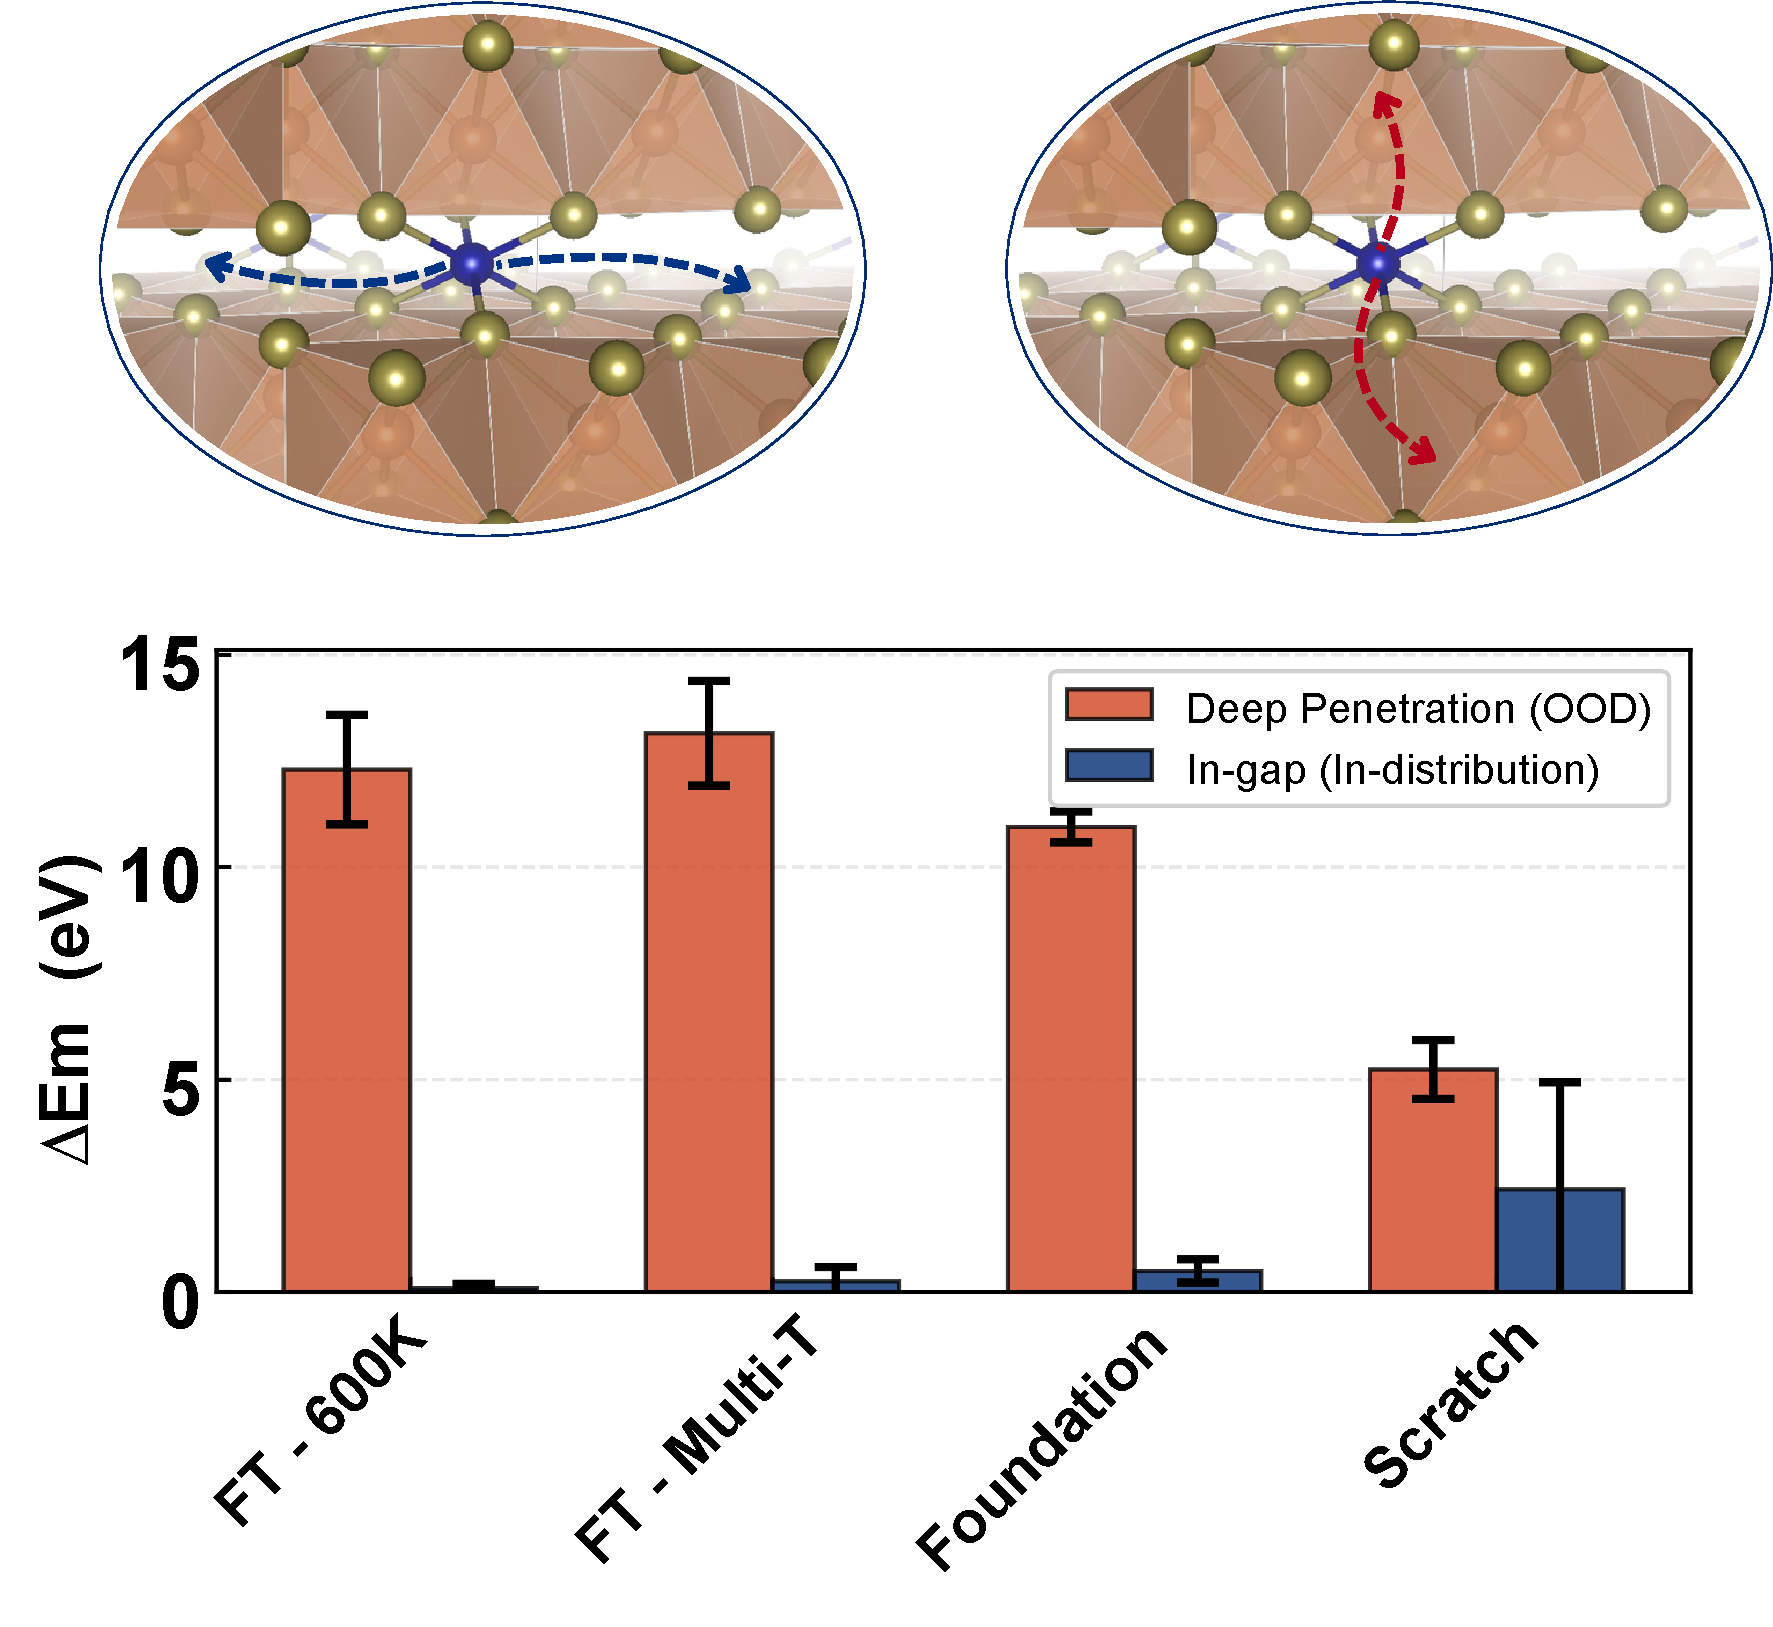
\includegraphics[width=\linewidth,height=0.42\textheight,keepaspectratio]{figure_pages/assets/fig_157.pdf}
\caption{Legacy published or conference-era benchmark figure retained for historical comparison. This page shows the candidate output ``Neurips2025 ai4mat em 1013'' within the audited LEGACY-NEURIPS family. The panel identity, source scope, and current status are retained in the accompanying evidence matrix.}
\label{fig:candidate_157}
\end{figure}
\textbf{Results text draft.} The figure is retained as an upstream reference asset. Its original protocol, data scope, and caption are not silently treated as identical to the Revision\textasciitilde{}1 audit.
\textbf{Discussion and boundary.} Use only when the manuscript explicitly labels the result as historical/upstream and states the protocol boundary.
\textbf{Article placement.} Proposed article location: Original main/SI manuscript.
\textbf{Reviewer linkage:} overall status NO\_DIRECT\_REVIEWER\_FIGURE\_LINK.
No direct reviewer-response figure linkage was identified; this page is retained for scientific/article audit rather than as a direct reviewer response.
\textbf{Evidence pointers.}
\begin{itemize}[leftmargin=1.4em,noitemsep]
\item Caption/text source: \begingroup\scriptsize\url{paper/paper/response_to_reviewers.log}\endgroup
\item Caption/text source: \begingroup\scriptsize\url{paper/paper/response_to_reviewers.out}\endgroup
\end{itemize}
\statusline{\textbf{Audit gap / next action:} Source-data and plotting provenance generally not co-located}
\vfill
\clearpage
\section{FIG-158 --- Neurips2025 ai4mat em si}
\label{figpage:fig-158}
\textbf{Group:} LEGACY-NEURIPS\quad \textbf{Evidence chain:} partial\quad \textbf{Status:} publication
\begin{figure}[H]
\centering
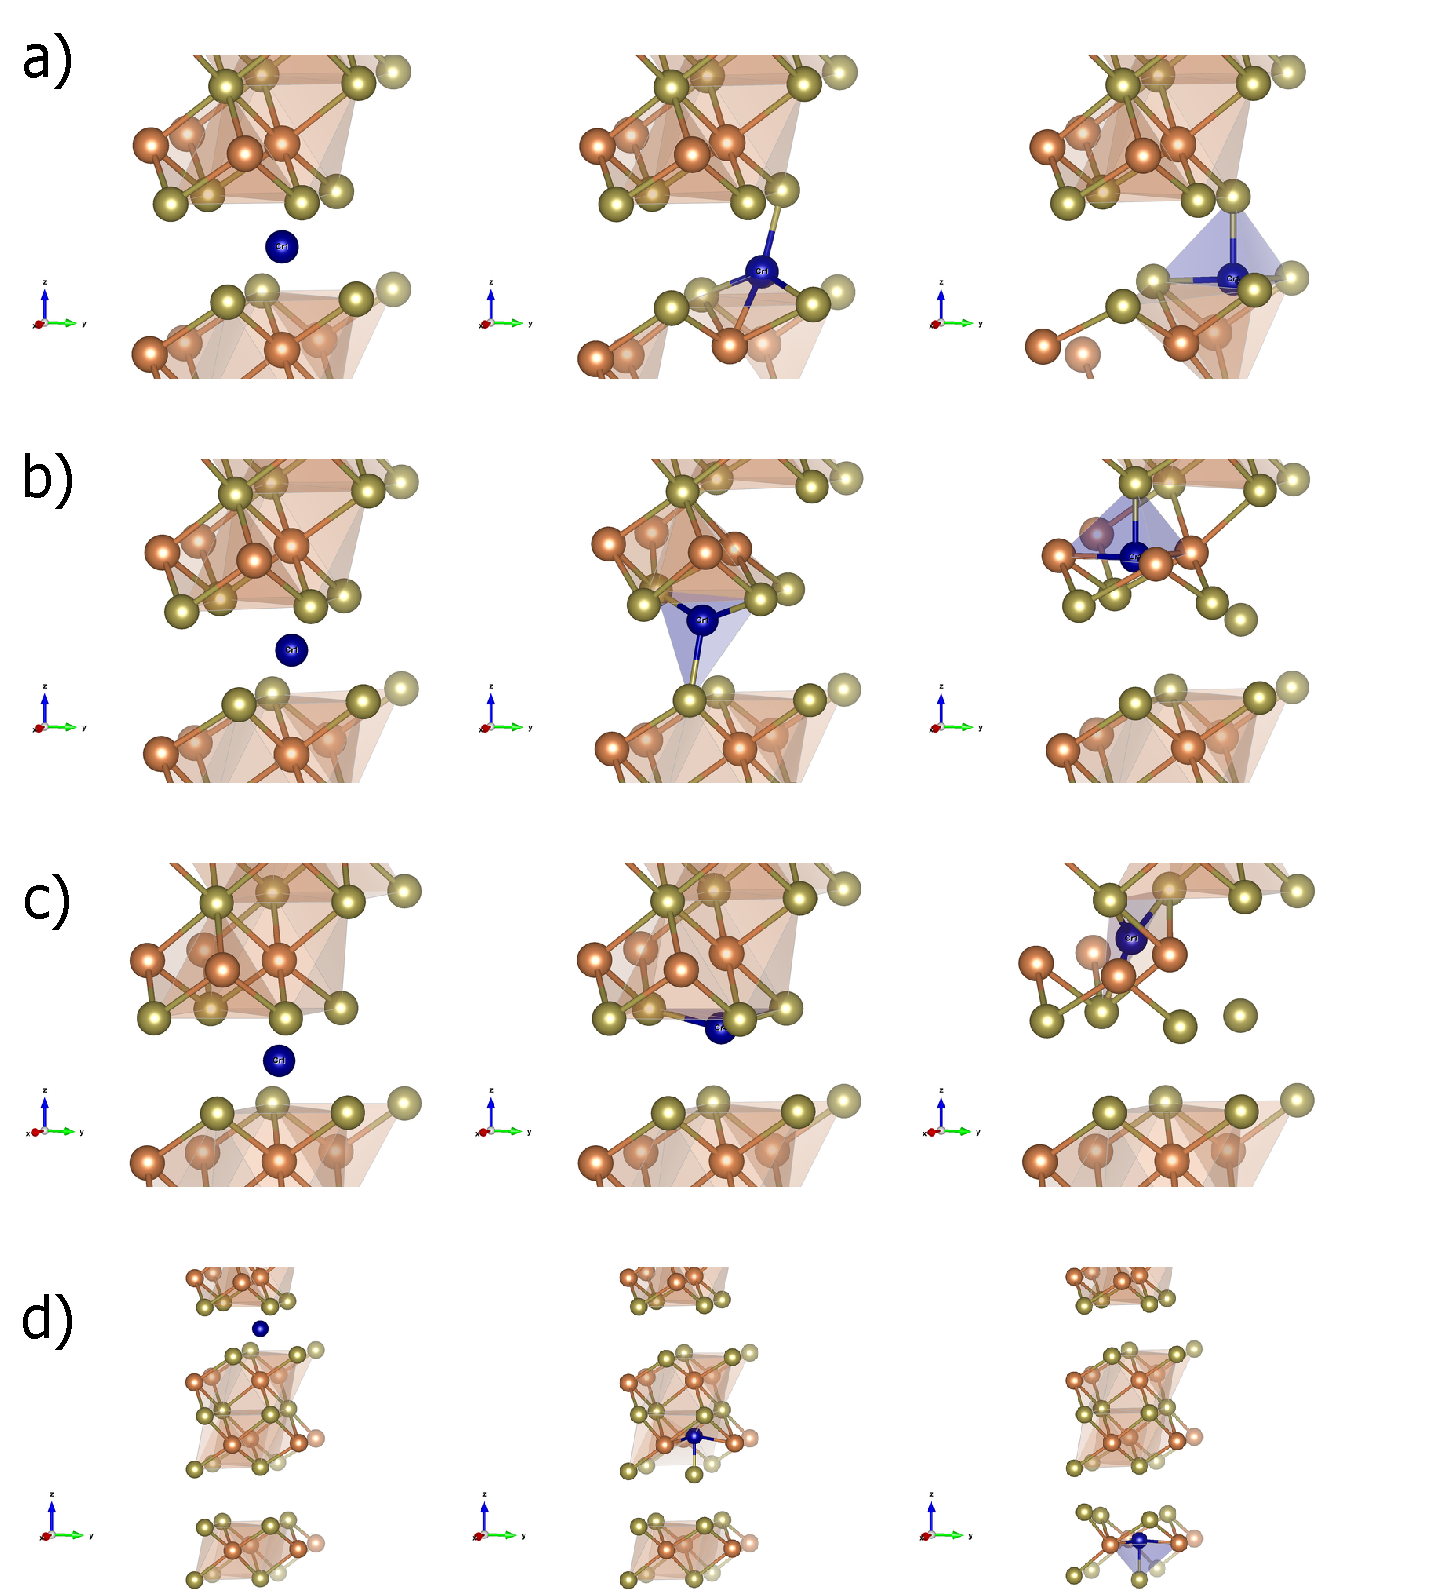
\includegraphics[width=\linewidth,height=0.42\textheight,keepaspectratio]{figure_pages/assets/fig_158.pdf}
\caption{Legacy published or conference-era benchmark figure retained for historical comparison. This page shows the candidate output ``Neurips2025 ai4mat em si'' within the audited LEGACY-NEURIPS family. The panel identity, source scope, and current status are retained in the accompanying evidence matrix.}
\label{fig:candidate_158}
\end{figure}
\textbf{Results text draft.} The figure is retained as an upstream reference asset. Its original protocol, data scope, and caption are not silently treated as identical to the Revision\textasciitilde{}1 audit.
\textbf{Discussion and boundary.} Use only when the manuscript explicitly labels the result as historical/upstream and states the protocol boundary.
\textbf{Article placement.} Proposed article location: Original main/SI manuscript.
\textbf{Reviewer linkage:} overall status NO\_DIRECT\_REVIEWER\_FIGURE\_LINK.
No direct reviewer-response figure linkage was identified; this page is retained for scientific/article audit rather than as a direct reviewer response.
\textbf{Evidence pointers.}
\begin{itemize}[leftmargin=1.4em,noitemsep]
\item Caption/text source: \begingroup\scriptsize\url{paper/paper/response_to_reviewers.log}\endgroup
\item Caption/text source: \begingroup\scriptsize\url{paper/paper/response_to_reviewers.out}\endgroup
\end{itemize}
\statusline{\textbf{Audit gap / next action:} Source-data and plotting provenance generally not co-located}
\vfill
\clearpage
\section{FIG-159 --- Neurips2025 ai4mat em main}
\label{figpage:fig-159}
\textbf{Group:} LEGACY-NEURIPS\quad \textbf{Evidence chain:} partial\quad \textbf{Status:} publication
\begin{figure}[H]
\centering
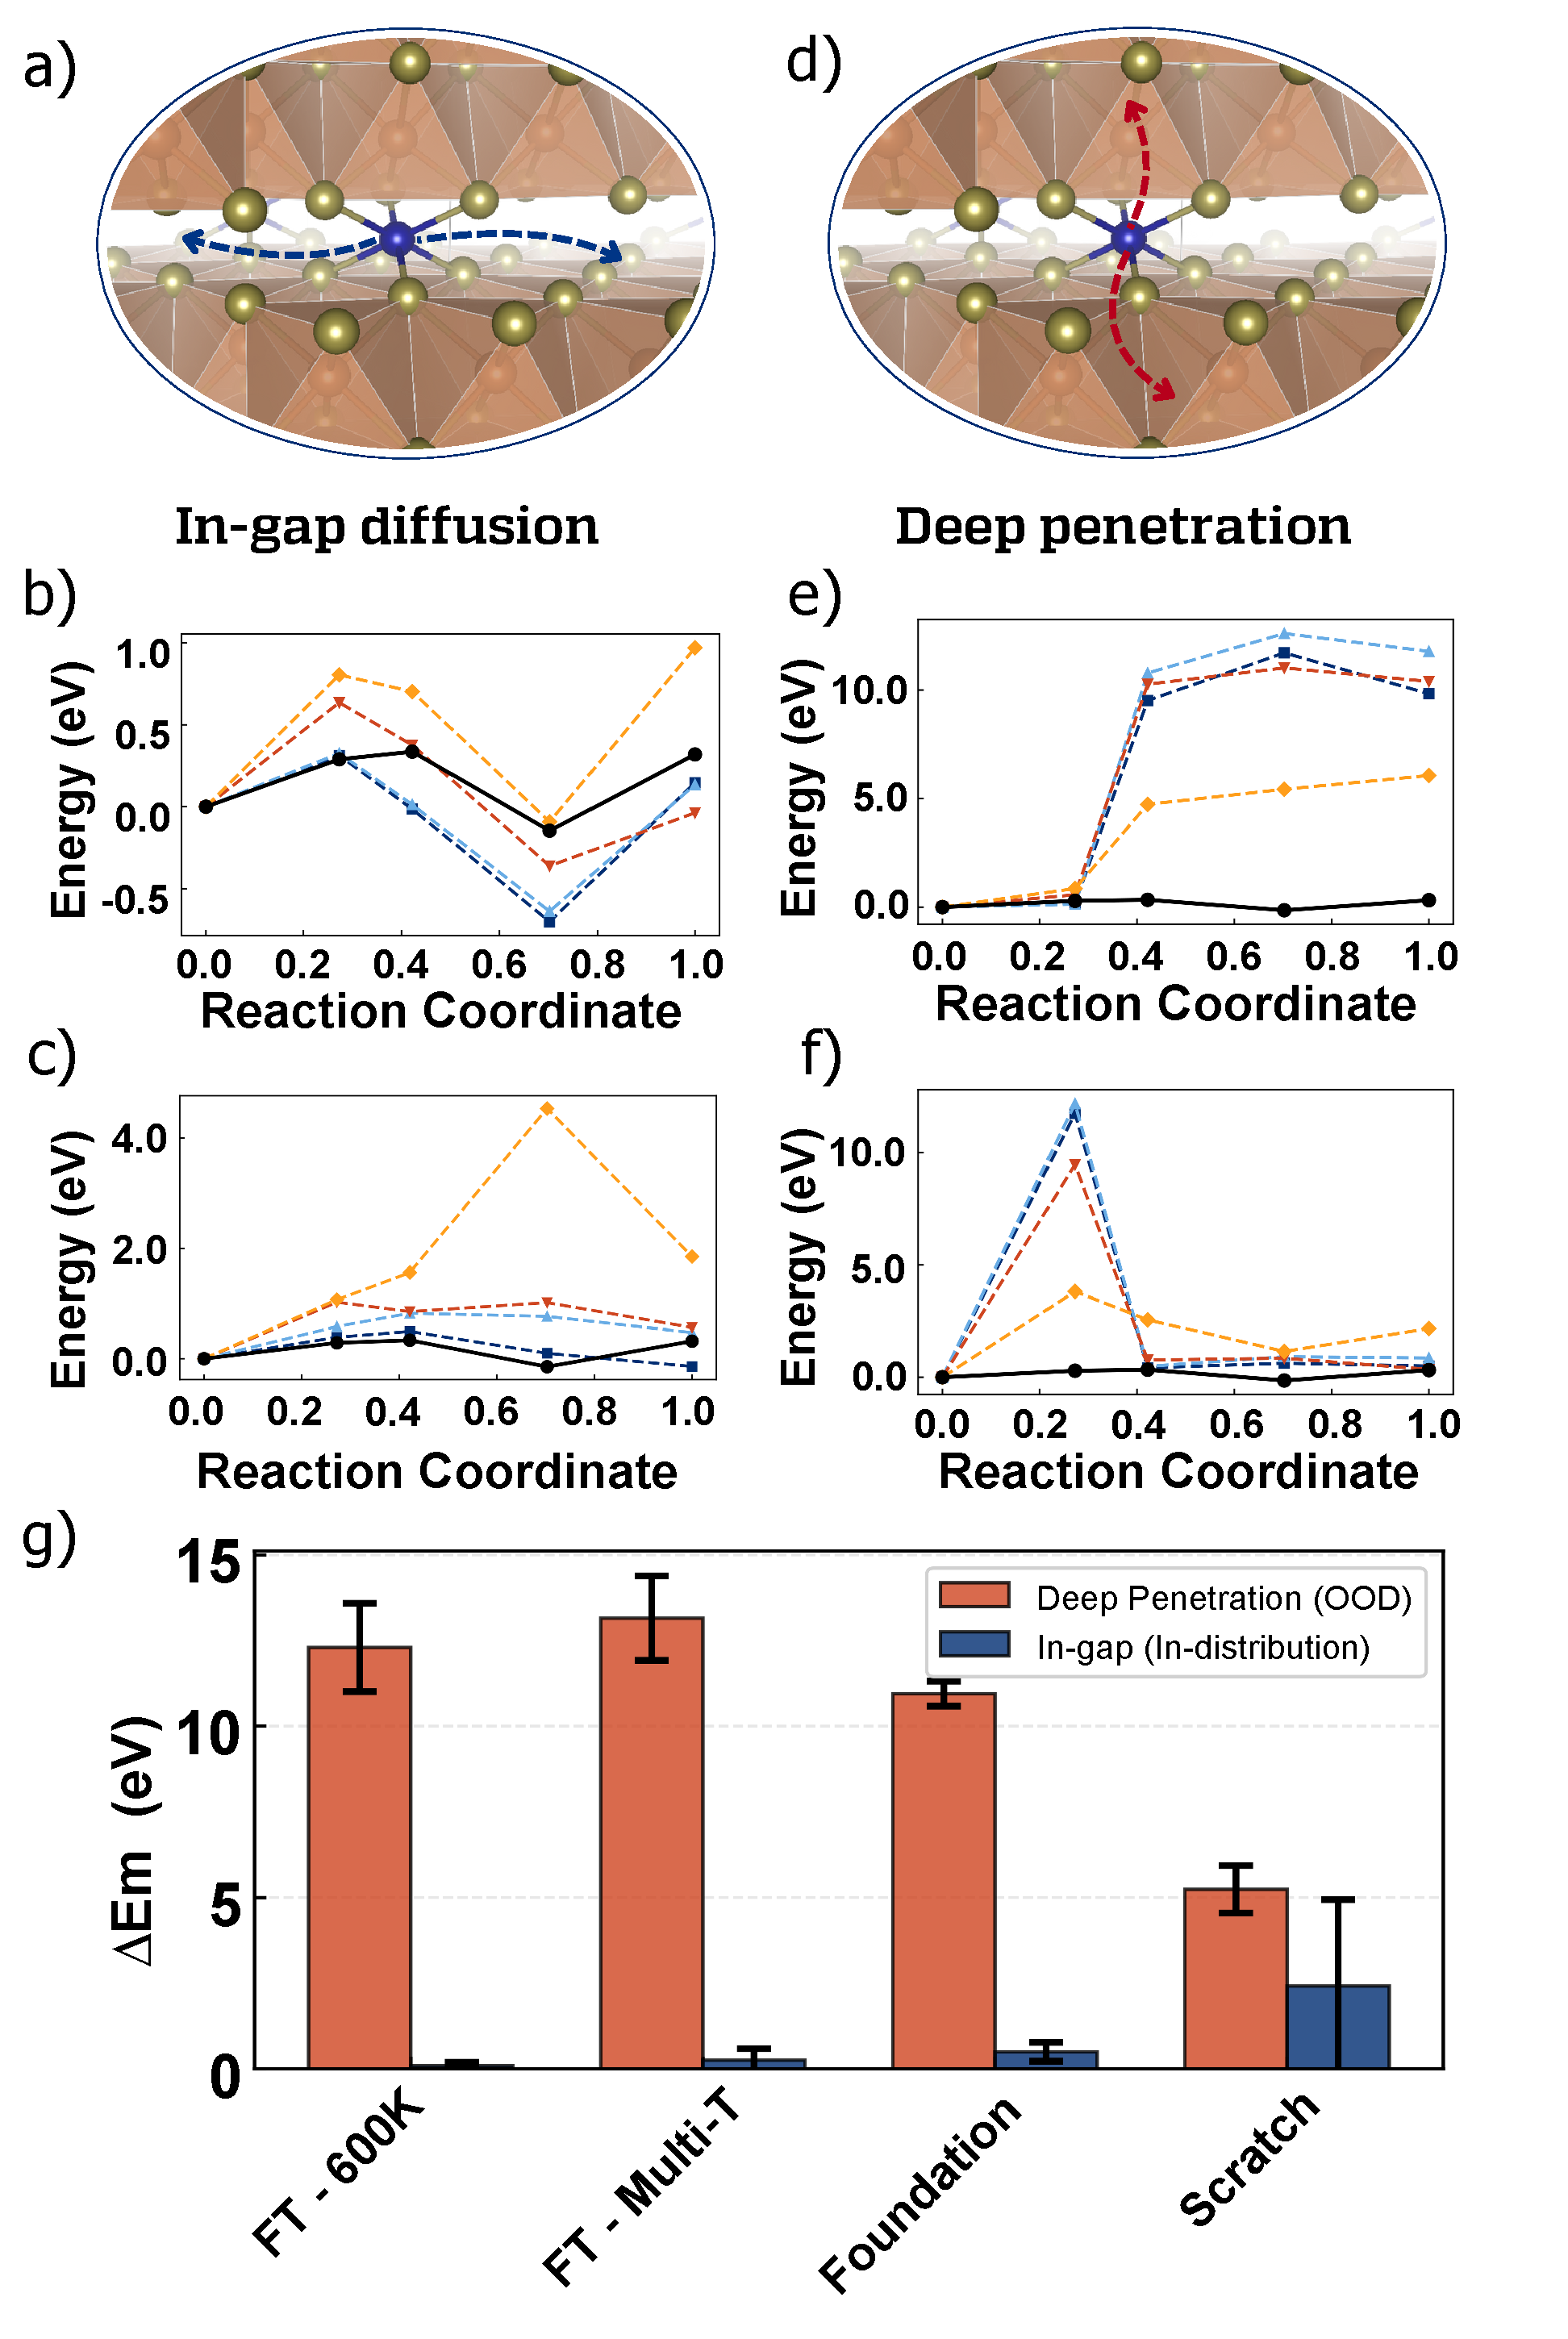
\includegraphics[width=\linewidth,height=0.42\textheight,keepaspectratio]{figure_pages/assets/fig_159.pdf}
\caption{Legacy published or conference-era benchmark figure retained for historical comparison. This page shows the candidate output ``Neurips2025 ai4mat em main'' within the audited LEGACY-NEURIPS family. The panel identity, source scope, and current status are retained in the accompanying evidence matrix.}
\label{fig:candidate_159}
\end{figure}
\textbf{Results text draft.} The figure is retained as an upstream reference asset. Its original protocol, data scope, and caption are not silently treated as identical to the Revision\textasciitilde{}1 audit.
\textbf{Discussion and boundary.} Use only when the manuscript explicitly labels the result as historical/upstream and states the protocol boundary.
\textbf{Article placement.} Proposed article location: Original main/SI manuscript.
\textbf{Reviewer linkage:} overall status NO\_DIRECT\_REVIEWER\_FIGURE\_LINK.
No direct reviewer-response figure linkage was identified; this page is retained for scientific/article audit rather than as a direct reviewer response.
\textbf{Evidence pointers.}
\begin{itemize}[leftmargin=1.4em,noitemsep]
\item Caption/text source: \begingroup\scriptsize\url{paper/paper/response_to_reviewers.log}\endgroup
\item Caption/text source: \begingroup\scriptsize\url{paper/paper/response_to_reviewers.out}\endgroup
\end{itemize}
\statusline{\textbf{Audit gap / next action:} Source-data and plotting provenance generally not co-located}
\vfill
\clearpage
\section{FIG-160 --- Neurips2025 ai4mat shap si}
\label{figpage:fig-160}
\textbf{Group:} LEGACY-NEURIPS\quad \textbf{Evidence chain:} partial\quad \textbf{Status:} publication
\begin{figure}[H]
\centering
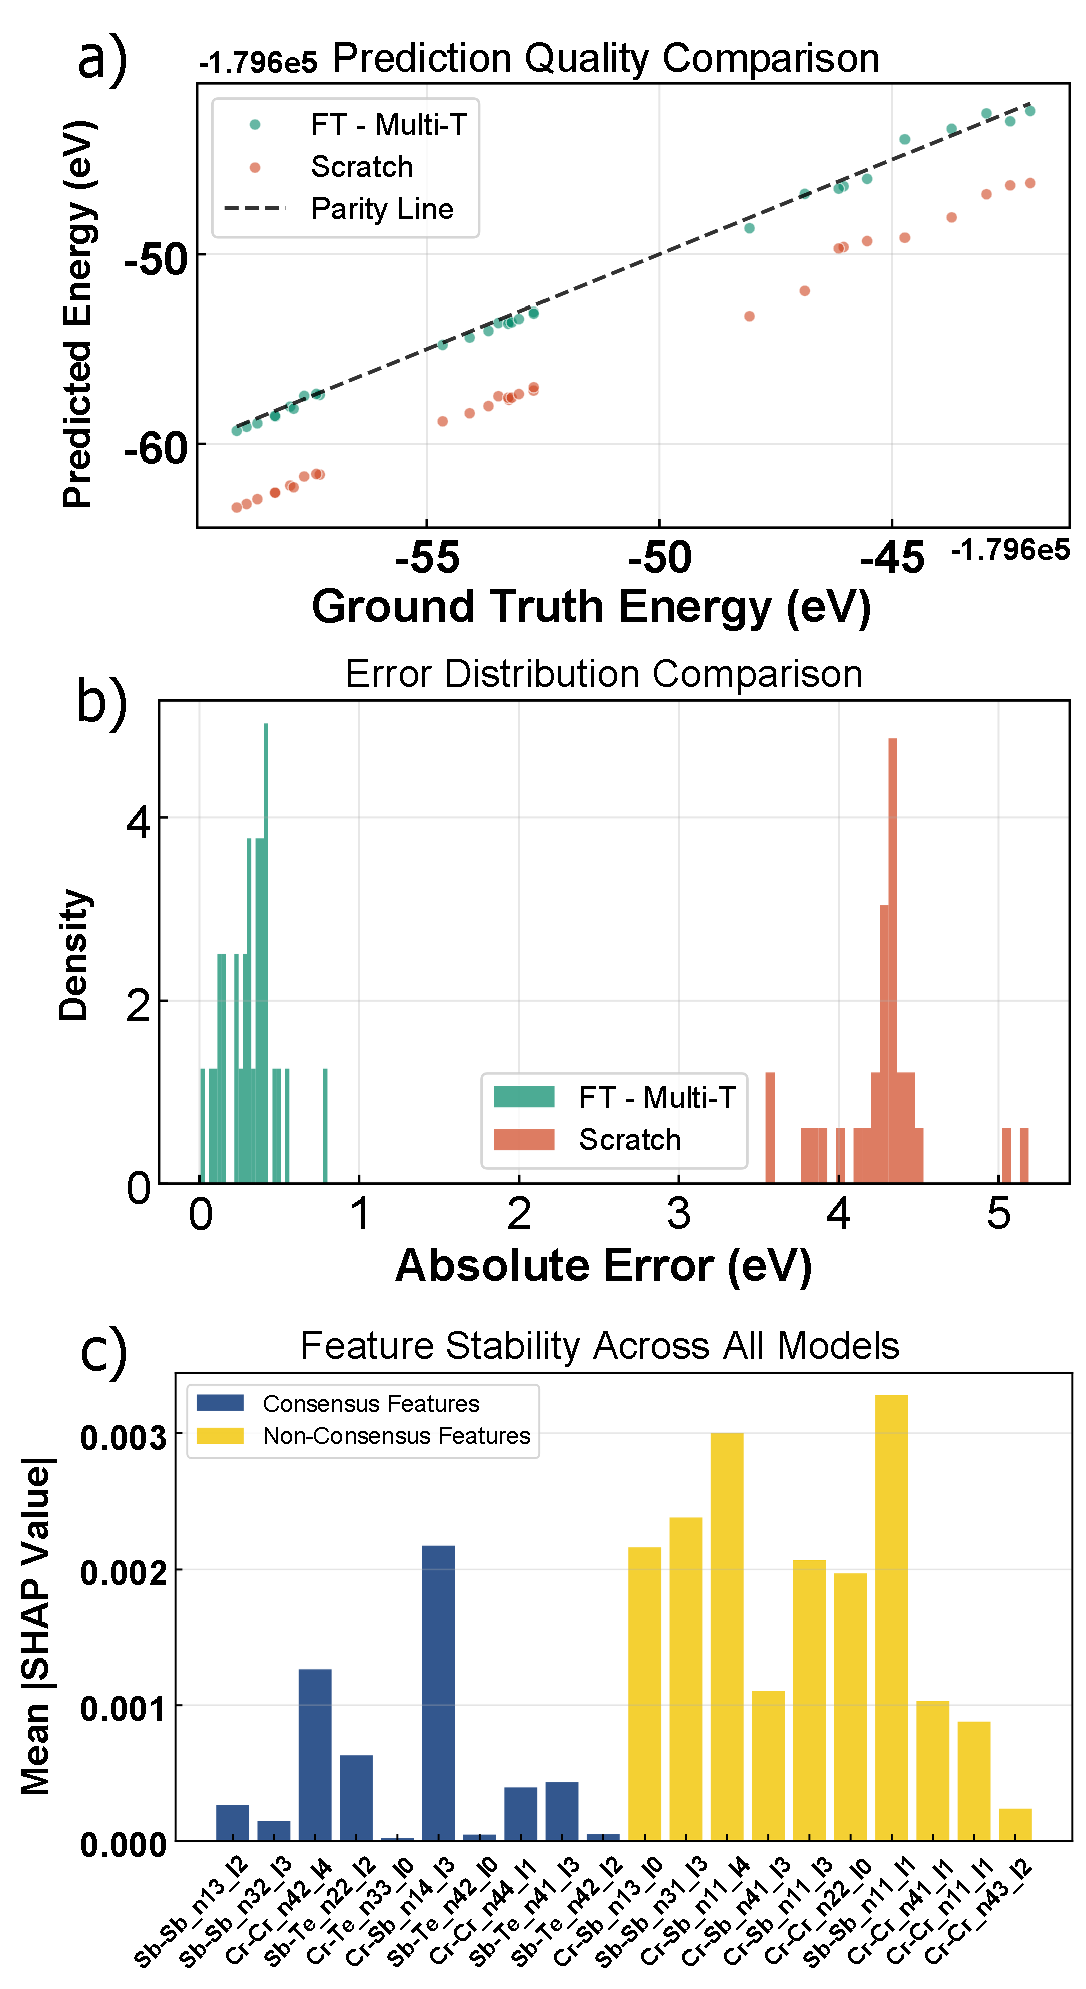
\includegraphics[width=\linewidth,height=0.42\textheight,keepaspectratio]{figure_pages/assets/fig_160.pdf}
\caption{Legacy published or conference-era benchmark figure retained for historical comparison. This page shows the candidate output ``Neurips2025 ai4mat shap si'' within the audited LEGACY-NEURIPS family. The panel identity, source scope, and current status are retained in the accompanying evidence matrix.}
\label{fig:candidate_160}
\end{figure}
\textbf{Results text draft.} The figure is retained as an upstream reference asset. Its original protocol, data scope, and caption are not silently treated as identical to the Revision\textasciitilde{}1 audit.
\textbf{Discussion and boundary.} Use only when the manuscript explicitly labels the result as historical/upstream and states the protocol boundary.
\textbf{Article placement.} Proposed article location: Original main/SI manuscript.
\textbf{Reviewer linkage:} overall status PARTIAL.
\begin{itemize}[leftmargin=1.4em,noitemsep]
\item \textbf{REV-A6 (PARTIAL):} Soften t-SNE/PHATE and SHAP interpretation claims and add projection/original-space and surrogate-fidelity checks. \emph{Completed:} Projection sensitivity, original-descriptor-space separation, and per-model cross-validated surrogate R2 are available; the text is scoped to descriptive/surrogate evidence. \emph{Still required:} A direct MACE Cr-Cr perturbation test remains pending if a causal claim about the dominant feature is desired; otherwise retain the surrogate-scoped wording.
\item \textbf{REV-C13 (PARTIAL):} Make the SHAP pipeline and advertised repository artifacts reproducible rather than leaving empty stubs. \emph{Completed:} The corrected SHAP inputs, scripts, lineage, and locked revised outputs are present for the declared three-model/150-frame scope. \emph{Still required:} Close the final release/empty-stub audit and reconcile the independent rerun with the locked historical CSV before claiming exact end-to-end regeneration.
\end{itemize}
\textbf{Evidence pointers.}
\begin{itemize}[leftmargin=1.4em,noitemsep]
\item Caption/text source: \begingroup\scriptsize\url{paper/paper/response_to_reviewers.log}\endgroup
\item Caption/text source: \begingroup\scriptsize\url{paper/paper/response_to_reviewers.out}\endgroup
\end{itemize}
\statusline{\textbf{Audit gap / next action:} Source-data and plotting provenance generally not co-located}
\vfill
\clearpage
\section{FIG-161 --- Neurips2025 ai4mat shap main}
\label{figpage:fig-161}
\textbf{Group:} LEGACY-NEURIPS\quad \textbf{Evidence chain:} partial\quad \textbf{Status:} publication
\begin{figure}[H]
\centering
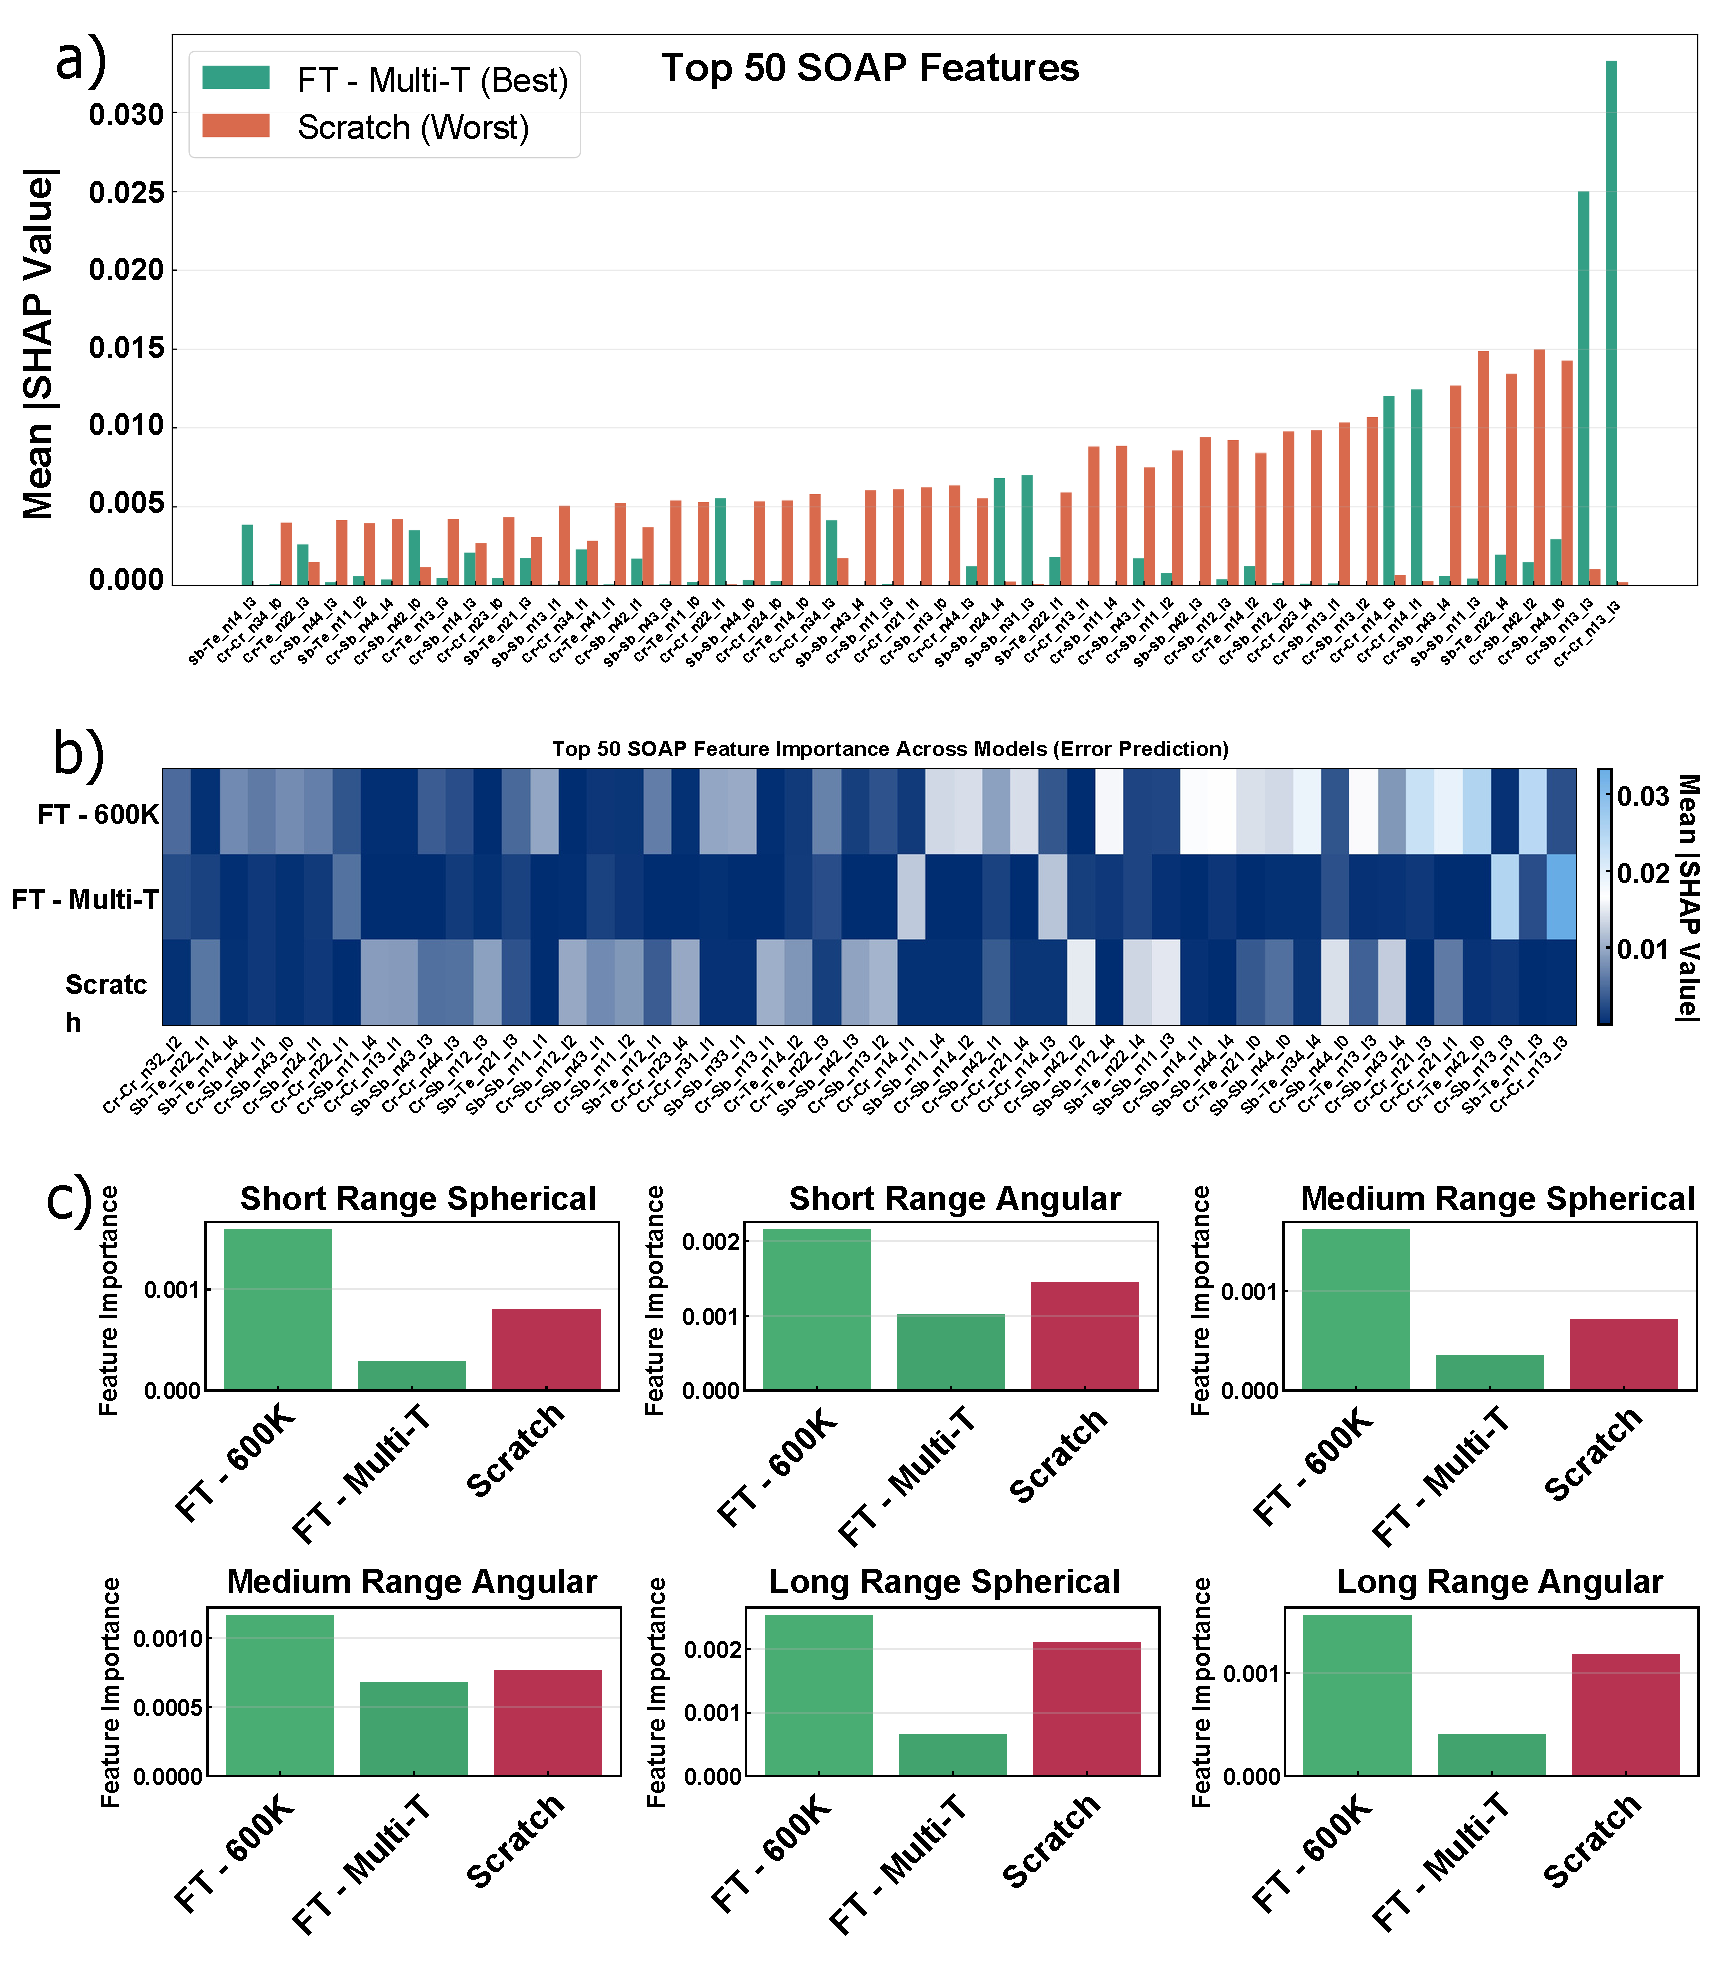
\includegraphics[width=\linewidth,height=0.42\textheight,keepaspectratio]{figure_pages/assets/fig_161.pdf}
\caption{Legacy published or conference-era benchmark figure retained for historical comparison. This page shows the candidate output ``Neurips2025 ai4mat shap main'' within the audited LEGACY-NEURIPS family. The panel identity, source scope, and current status are retained in the accompanying evidence matrix.}
\label{fig:candidate_161}
\end{figure}
\textbf{Results text draft.} The figure is retained as an upstream reference asset. Its original protocol, data scope, and caption are not silently treated as identical to the Revision\textasciitilde{}1 audit.
\textbf{Discussion and boundary.} Use only when the manuscript explicitly labels the result as historical/upstream and states the protocol boundary.
\textbf{Article placement.} Proposed article location: Original main/SI manuscript.
\textbf{Reviewer linkage:} overall status PARTIAL.
\begin{itemize}[leftmargin=1.4em,noitemsep]
\item \textbf{REV-A6 (PARTIAL):} Soften t-SNE/PHATE and SHAP interpretation claims and add projection/original-space and surrogate-fidelity checks. \emph{Completed:} Projection sensitivity, original-descriptor-space separation, and per-model cross-validated surrogate R2 are available; the text is scoped to descriptive/surrogate evidence. \emph{Still required:} A direct MACE Cr-Cr perturbation test remains pending if a causal claim about the dominant feature is desired; otherwise retain the surrogate-scoped wording.
\item \textbf{REV-C13 (PARTIAL):} Make the SHAP pipeline and advertised repository artifacts reproducible rather than leaving empty stubs. \emph{Completed:} The corrected SHAP inputs, scripts, lineage, and locked revised outputs are present for the declared three-model/150-frame scope. \emph{Still required:} Close the final release/empty-stub audit and reconcile the independent rerun with the locked historical CSV before claiming exact end-to-end regeneration.
\end{itemize}
\textbf{Evidence pointers.}
\begin{itemize}[leftmargin=1.4em,noitemsep]
\item Caption/text source: \begingroup\scriptsize\url{paper/paper/response_to_reviewers.log}\endgroup
\item Caption/text source: \begingroup\scriptsize\url{paper/paper/response_to_reviewers.out}\endgroup
\end{itemize}
\statusline{\textbf{Audit gap / next action:} Source-data and plotting provenance generally not co-located}
\vfill
\clearpage
\section{FIG-162 --- Neurips2025 ai4mat shap main2}
\label{figpage:fig-162}
\textbf{Group:} LEGACY-NEURIPS\quad \textbf{Evidence chain:} partial\quad \textbf{Status:} publication
\begin{figure}[H]
\centering
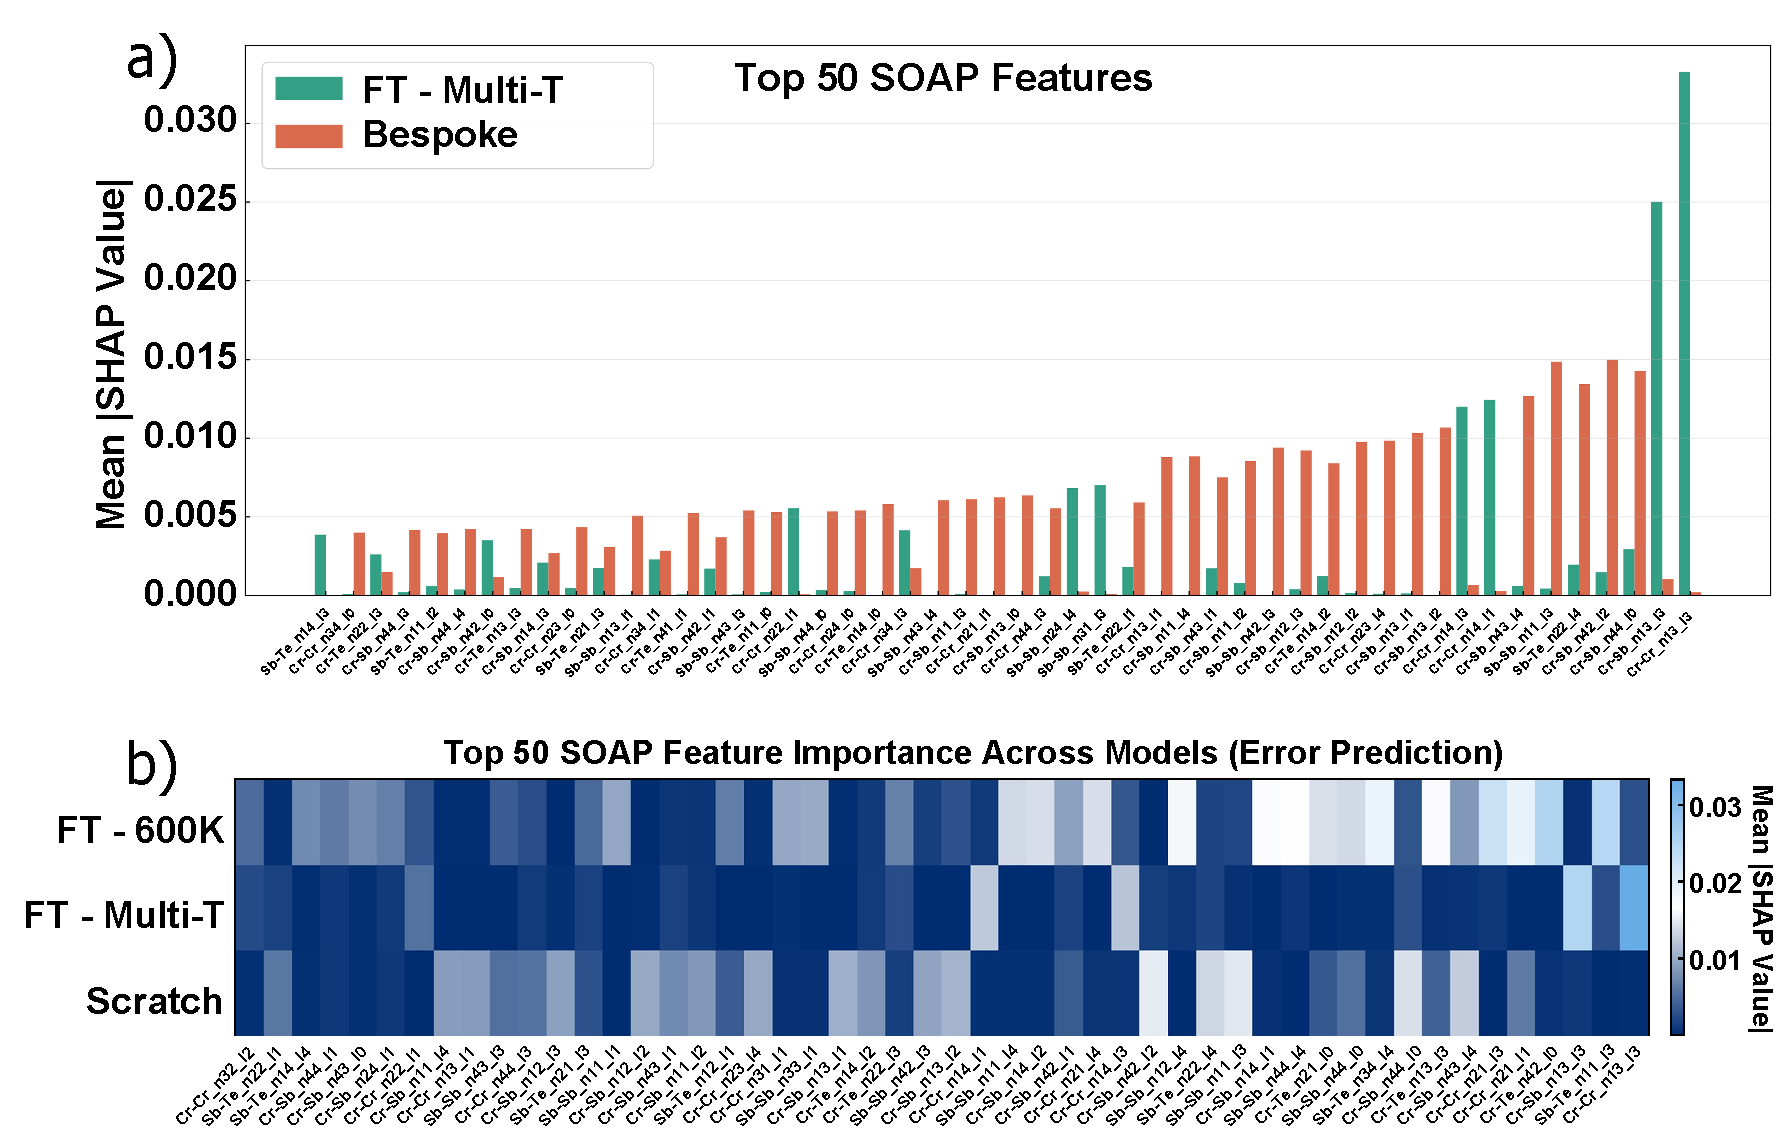
\includegraphics[width=\linewidth,height=0.42\textheight,keepaspectratio]{figure_pages/assets/fig_162.pdf}
\caption{Legacy published or conference-era benchmark figure retained for historical comparison. This page shows the candidate output ``Neurips2025 ai4mat shap main2'' within the audited LEGACY-NEURIPS family. The panel identity, source scope, and current status are retained in the accompanying evidence matrix.}
\label{fig:candidate_162}
\end{figure}
\textbf{Results text draft.} The figure is retained as an upstream reference asset. Its original protocol, data scope, and caption are not silently treated as identical to the Revision\textasciitilde{}1 audit.
\textbf{Discussion and boundary.} Use only when the manuscript explicitly labels the result as historical/upstream and states the protocol boundary.
\textbf{Article placement.} Proposed article location: Original main/SI manuscript.
\textbf{Reviewer linkage:} overall status PARTIAL.
\begin{itemize}[leftmargin=1.4em,noitemsep]
\item \textbf{REV-A6 (PARTIAL):} Soften t-SNE/PHATE and SHAP interpretation claims and add projection/original-space and surrogate-fidelity checks. \emph{Completed:} Projection sensitivity, original-descriptor-space separation, and per-model cross-validated surrogate R2 are available; the text is scoped to descriptive/surrogate evidence. \emph{Still required:} A direct MACE Cr-Cr perturbation test remains pending if a causal claim about the dominant feature is desired; otherwise retain the surrogate-scoped wording.
\item \textbf{REV-C13 (PARTIAL):} Make the SHAP pipeline and advertised repository artifacts reproducible rather than leaving empty stubs. \emph{Completed:} The corrected SHAP inputs, scripts, lineage, and locked revised outputs are present for the declared three-model/150-frame scope. \emph{Still required:} Close the final release/empty-stub audit and reconcile the independent rerun with the locked historical CSV before claiming exact end-to-end regeneration.
\end{itemize}
\textbf{Evidence pointers.}
\begin{itemize}[leftmargin=1.4em,noitemsep]
\item Caption/text source: \begingroup\scriptsize\url{paper/paper/response_to_reviewers.log}\endgroup
\item Caption/text source: \begingroup\scriptsize\url{paper/paper/response_to_reviewers.out}\endgroup
\end{itemize}
\statusline{\textbf{Audit gap / next action:} Source-data and plotting provenance generally not co-located}
\vfill
\clearpage
\section{FIG-163 --- Neurips2025 ai4mat si1}
\label{figpage:fig-163}
\textbf{Group:} LEGACY-NEURIPS\quad \textbf{Evidence chain:} partial\quad \textbf{Status:} publication
\begin{figure}[H]
\centering
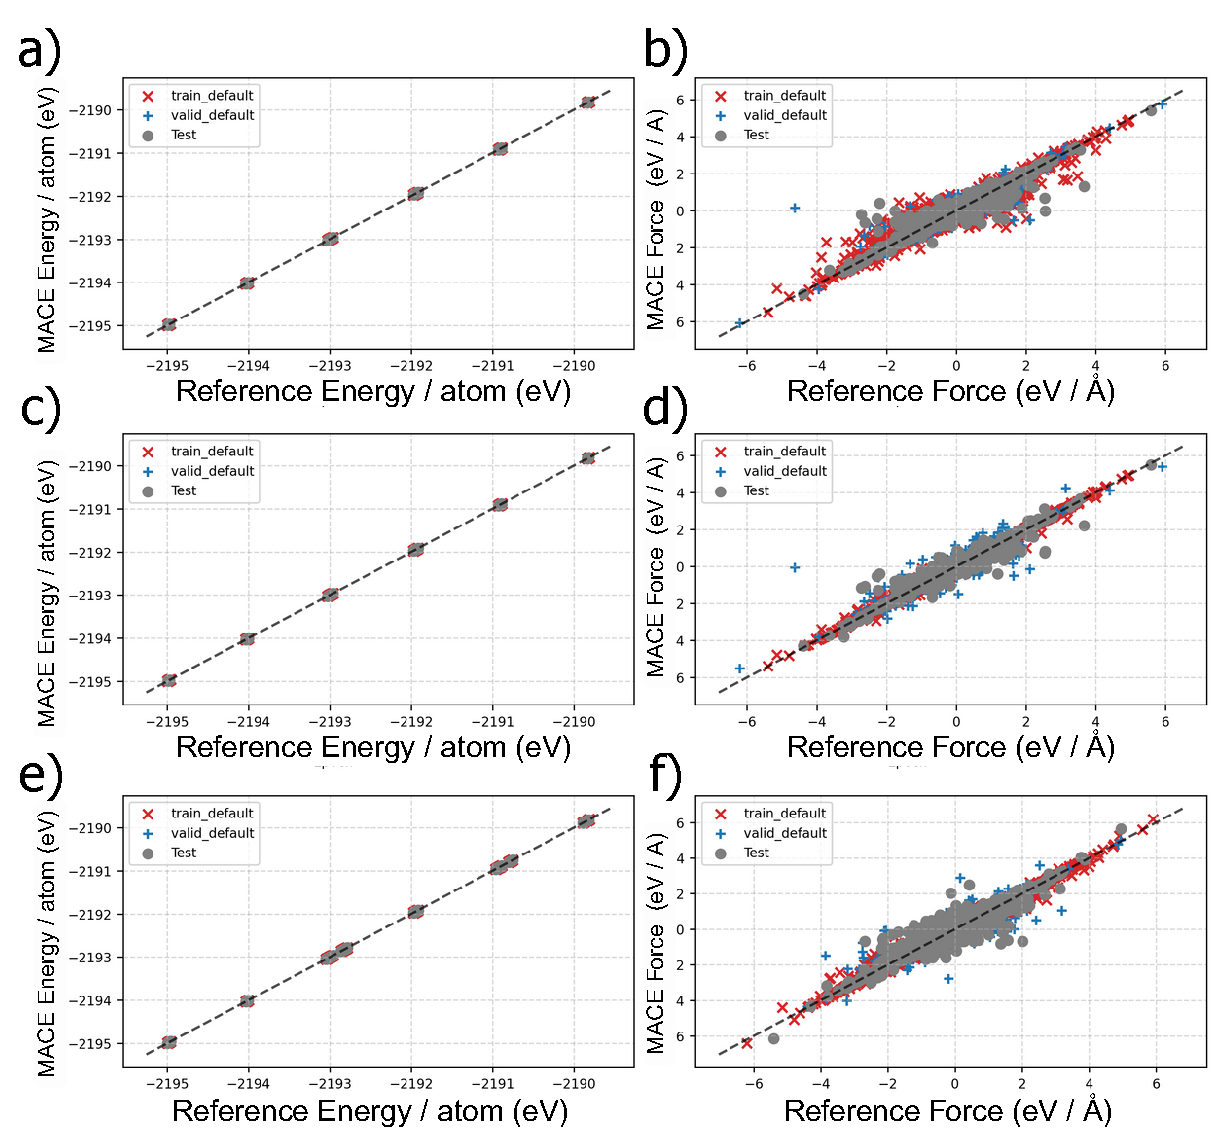
\includegraphics[width=\linewidth,height=0.42\textheight,keepaspectratio]{figure_pages/assets/fig_163.pdf}
\caption{Legacy published or conference-era benchmark figure retained for historical comparison. This page shows the candidate output ``Neurips2025 ai4mat si1'' within the audited LEGACY-NEURIPS family. The panel identity, source scope, and current status are retained in the accompanying evidence matrix.}
\label{fig:candidate_163}
\end{figure}
\textbf{Results text draft.} The figure is retained as an upstream reference asset. Its original protocol, data scope, and caption are not silently treated as identical to the Revision\textasciitilde{}1 audit.
\textbf{Discussion and boundary.} Use only when the manuscript explicitly labels the result as historical/upstream and states the protocol boundary.
\textbf{Article placement.} Proposed article location: Original main/SI manuscript.
\textbf{Reviewer linkage:} overall status NO\_DIRECT\_REVIEWER\_FIGURE\_LINK.
No direct reviewer-response figure linkage was identified; this page is retained for scientific/article audit rather than as a direct reviewer response.
\textbf{Evidence pointers.}
\begin{itemize}[leftmargin=1.4em,noitemsep]
\item Caption/text source: \begingroup\scriptsize\url{paper/paper/response_to_reviewers.log}\endgroup
\item Caption/text source: \begingroup\scriptsize\url{paper/paper/response_to_reviewers.out}\endgroup
\end{itemize}
\statusline{\textbf{Audit gap / next action:} Source-data and plotting provenance generally not co-located}
\vfill
\clearpage
\section{FIG-164 --- Neurips2025 ai4mat si2}
\label{figpage:fig-164}
\textbf{Group:} LEGACY-NEURIPS\quad \textbf{Evidence chain:} partial\quad \textbf{Status:} publication
\begin{figure}[H]
\centering
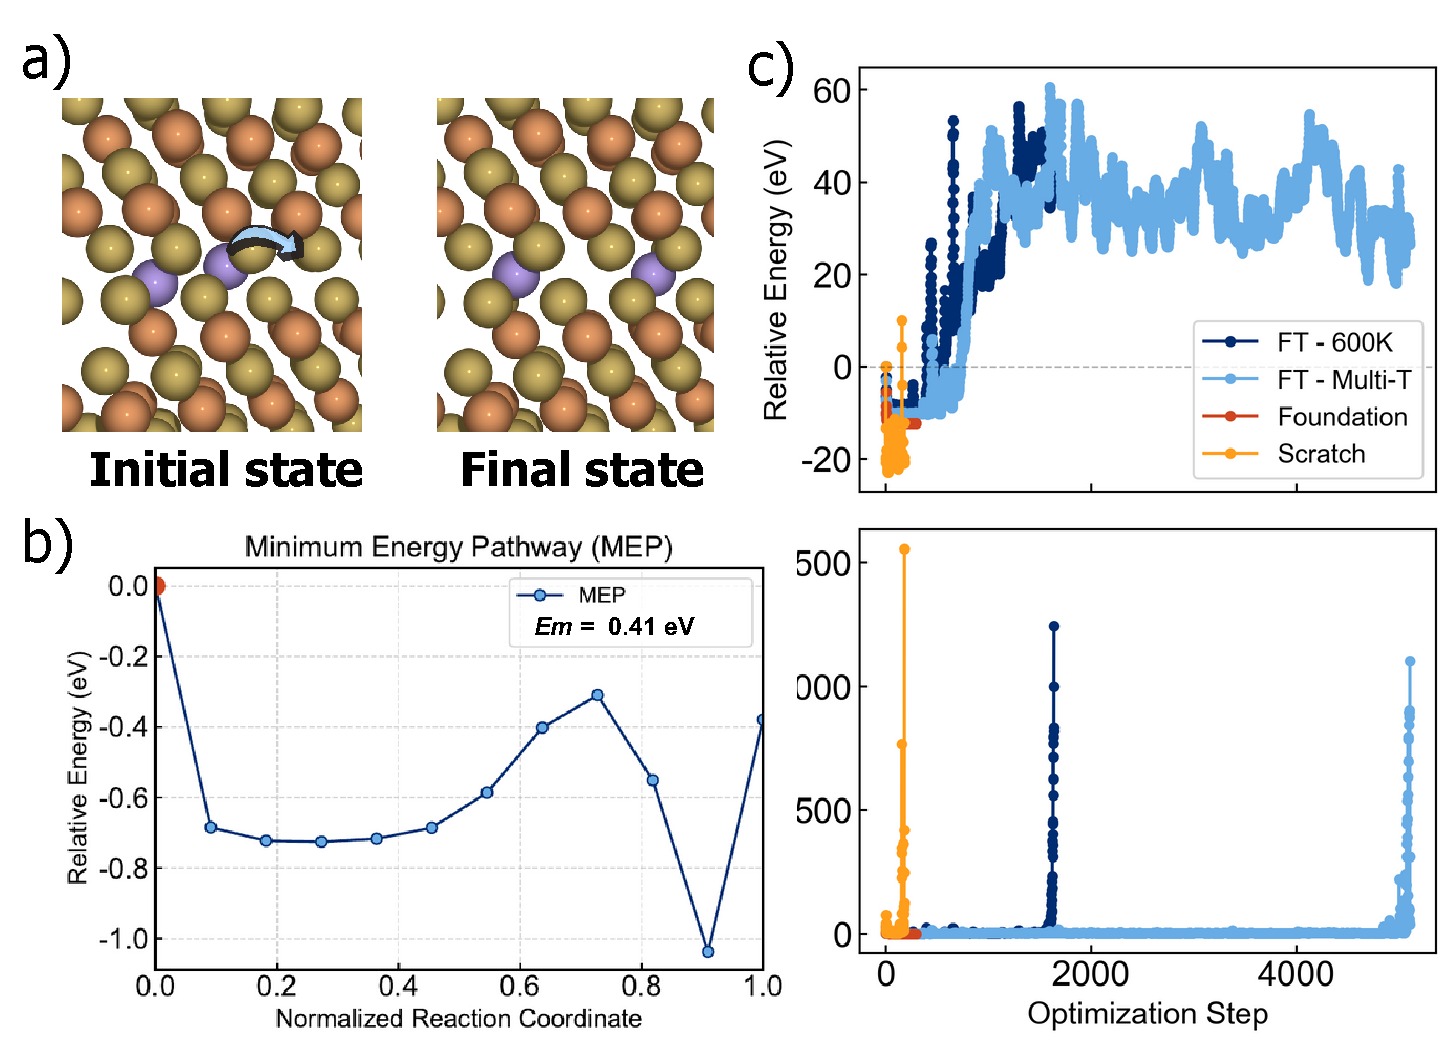
\includegraphics[width=\linewidth,height=0.42\textheight,keepaspectratio]{figure_pages/assets/fig_164.pdf}
\caption{Legacy published or conference-era benchmark figure retained for historical comparison. This page shows the candidate output ``Neurips2025 ai4mat si2'' within the audited LEGACY-NEURIPS family. The panel identity, source scope, and current status are retained in the accompanying evidence matrix.}
\label{fig:candidate_164}
\end{figure}
\textbf{Results text draft.} The figure is retained as an upstream reference asset. Its original protocol, data scope, and caption are not silently treated as identical to the Revision\textasciitilde{}1 audit.
\textbf{Discussion and boundary.} Use only when the manuscript explicitly labels the result as historical/upstream and states the protocol boundary.
\textbf{Article placement.} Proposed article location: Original main/SI manuscript.
\textbf{Reviewer linkage:} overall status NO\_DIRECT\_REVIEWER\_FIGURE\_LINK.
No direct reviewer-response figure linkage was identified; this page is retained for scientific/article audit rather than as a direct reviewer response.
\textbf{Evidence pointers.}
\begin{itemize}[leftmargin=1.4em,noitemsep]
\item Caption/text source: \begingroup\scriptsize\url{paper/paper/response_to_reviewers.log}\endgroup
\item Caption/text source: \begingroup\scriptsize\url{paper/paper/response_to_reviewers.out}\endgroup
\end{itemize}
\statusline{\textbf{Audit gap / next action:} Source-data and plotting provenance generally not co-located}
\vfill
\clearpage
\section{FIG-165 --- Neurips2025 ai4mat fig1 schematic}
\label{figpage:fig-165}
\textbf{Group:} LEGACY-NEURIPS\quad \textbf{Evidence chain:} partial\quad \textbf{Status:} publication
\begin{figure}[H]
\centering
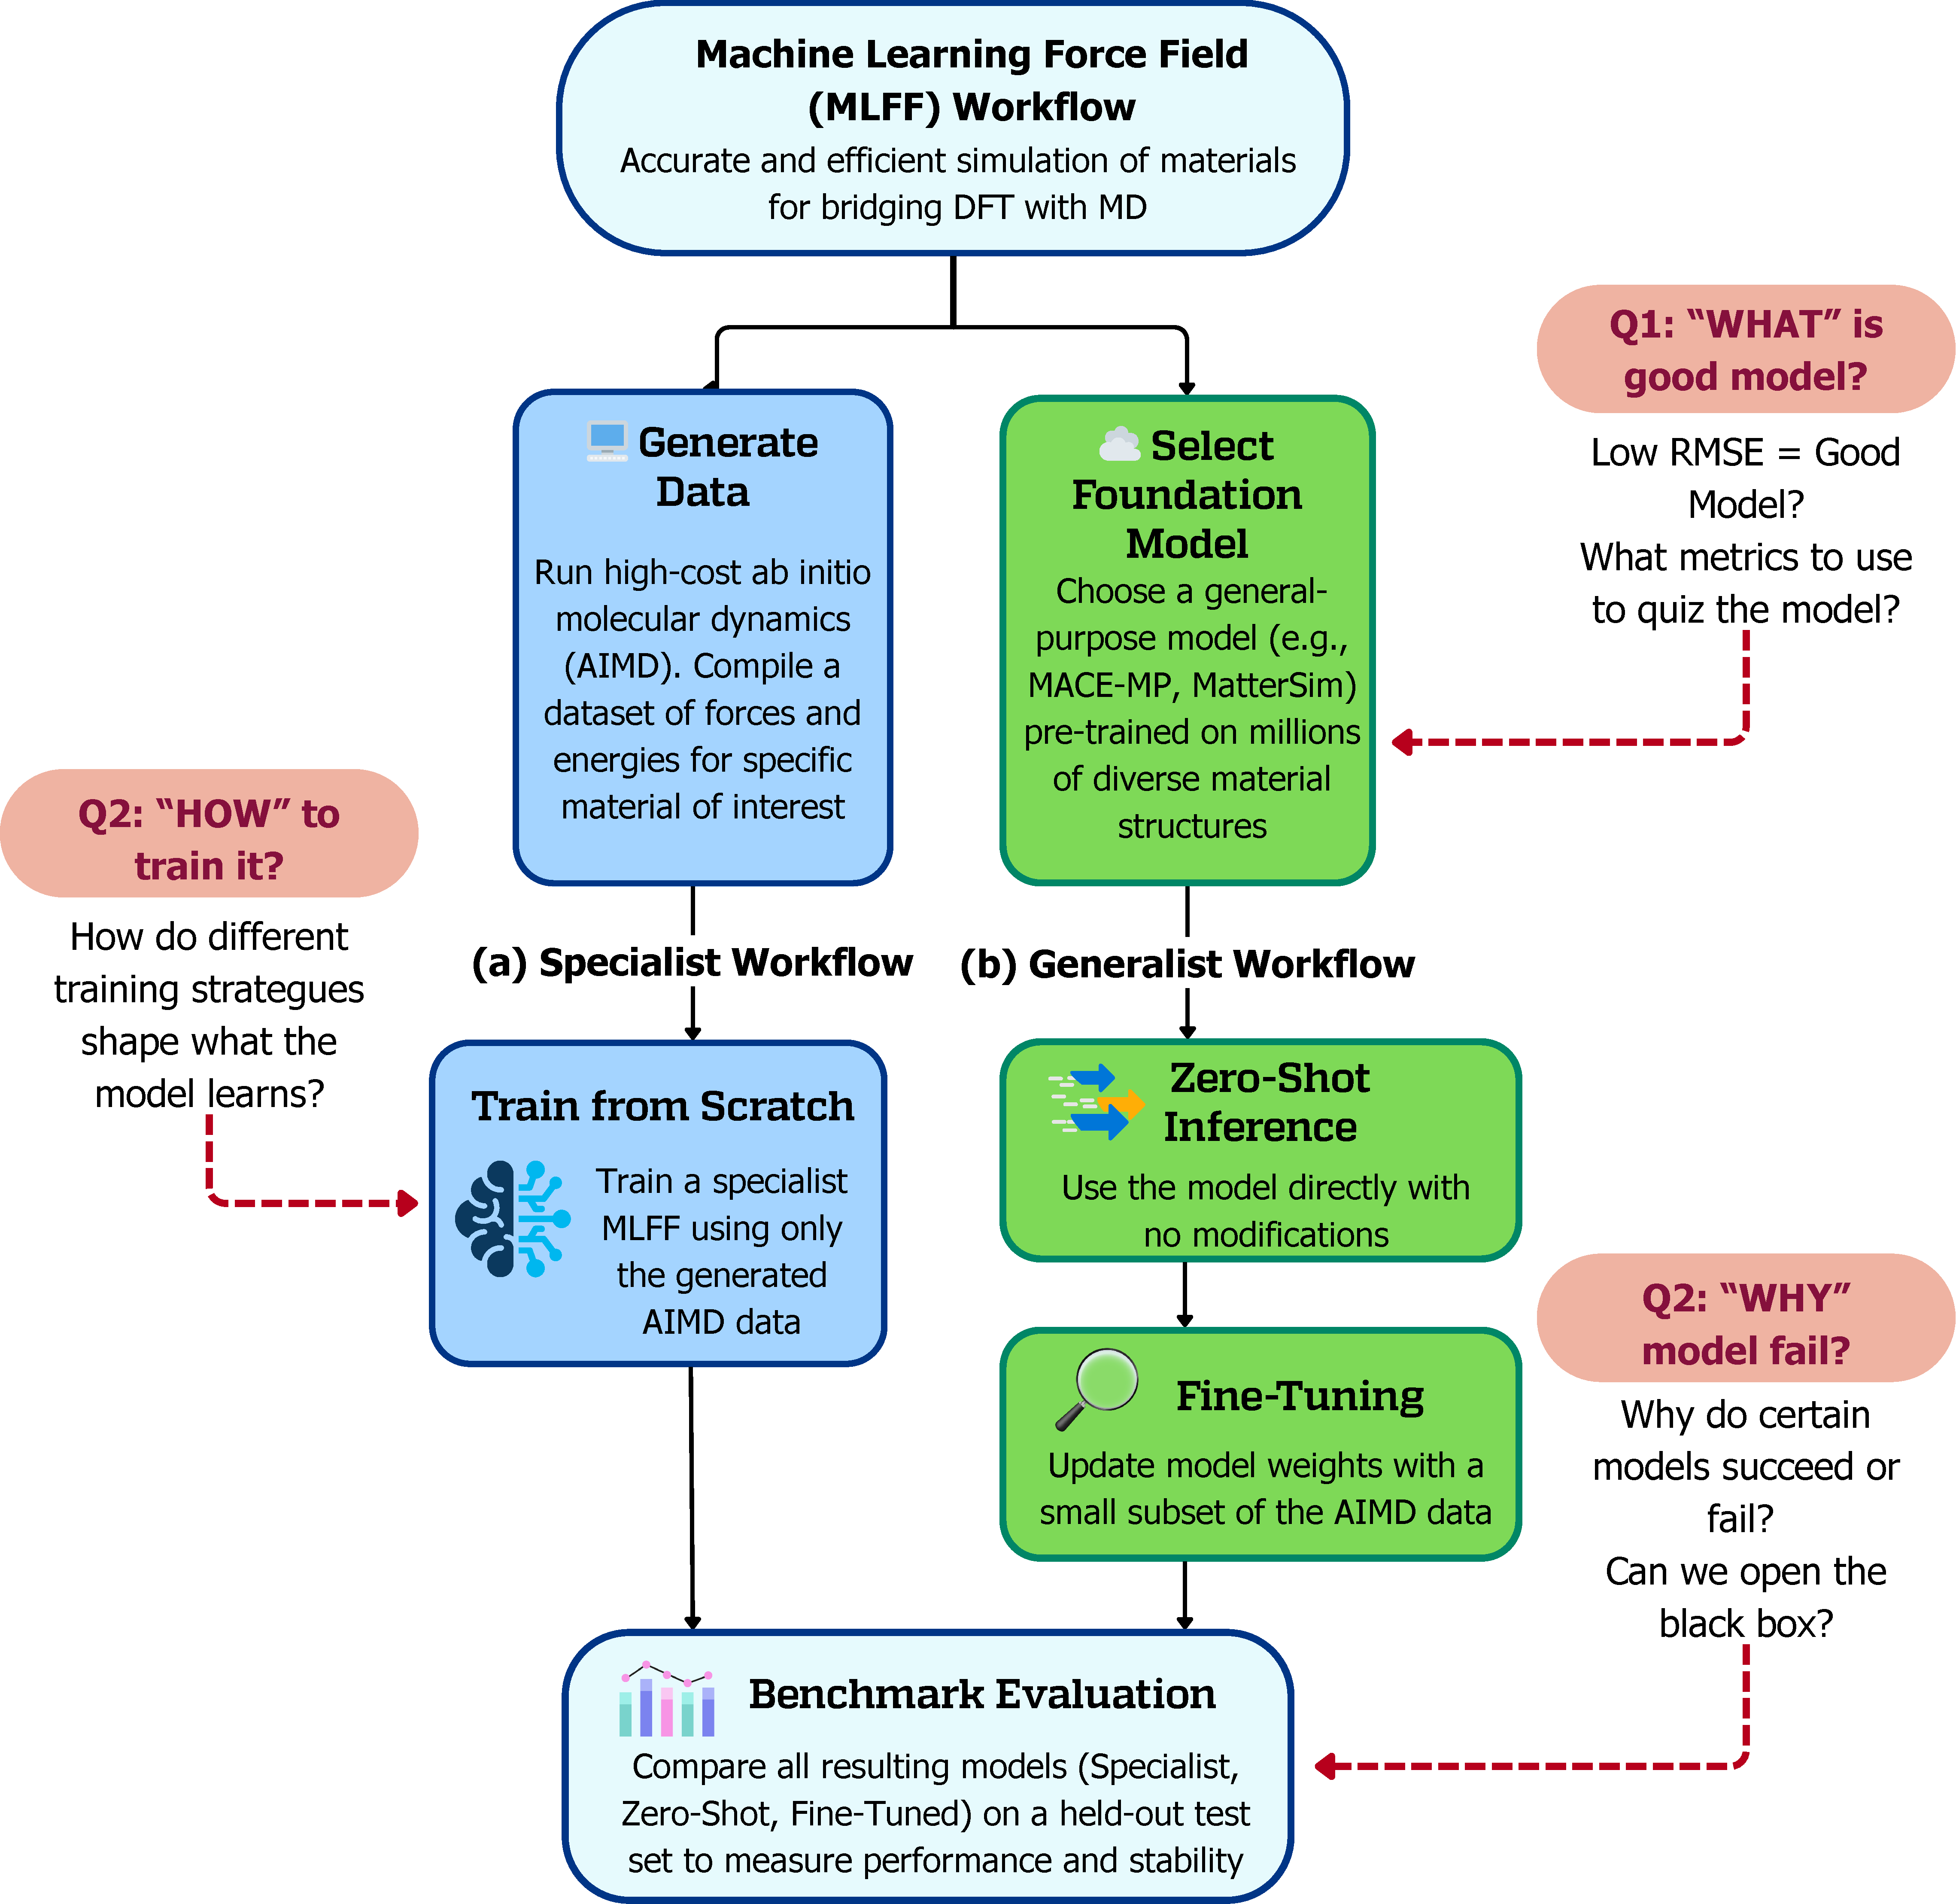
\includegraphics[width=\linewidth,height=0.42\textheight,keepaspectratio]{figure_pages/assets/fig_165.pdf}
\caption{Legacy published or conference-era benchmark figure retained for historical comparison. This page shows the candidate output ``Neurips2025 ai4mat fig1 schematic'' within the audited LEGACY-NEURIPS family. The panel identity, source scope, and current status are retained in the accompanying evidence matrix.}
\label{fig:candidate_165}
\end{figure}
\textbf{Results text draft.} The figure is retained as an upstream reference asset. Its original protocol, data scope, and caption are not silently treated as identical to the Revision\textasciitilde{}1 audit.
\textbf{Discussion and boundary.} Use only when the manuscript explicitly labels the result as historical/upstream and states the protocol boundary.
\textbf{Article placement.} Proposed article location: Original main/SI manuscript.
\textbf{Reviewer linkage:} overall status NO\_DIRECT\_REVIEWER\_FIGURE\_LINK.
No direct reviewer-response figure linkage was identified; this page is retained for scientific/article audit rather than as a direct reviewer response.
\textbf{Evidence pointers.}
\begin{itemize}[leftmargin=1.4em,noitemsep]
\item Caption/text source: \begingroup\scriptsize\url{paper/paper/response_to_reviewers.log}\endgroup
\item Caption/text source: \begingroup\scriptsize\url{paper/paper/response_to_reviewers.out}\endgroup
\end{itemize}
\statusline{\textbf{Audit gap / next action:} Source-data and plotting provenance generally not co-located}
\vfill
\clearpage
\section{FIG-166 --- Neurips2025 ai4mat fig2 v2}
\label{figpage:fig-166}
\textbf{Group:} LEGACY-NEURIPS\quad \textbf{Evidence chain:} partial\quad \textbf{Status:} publication
\begin{figure}[H]
\centering
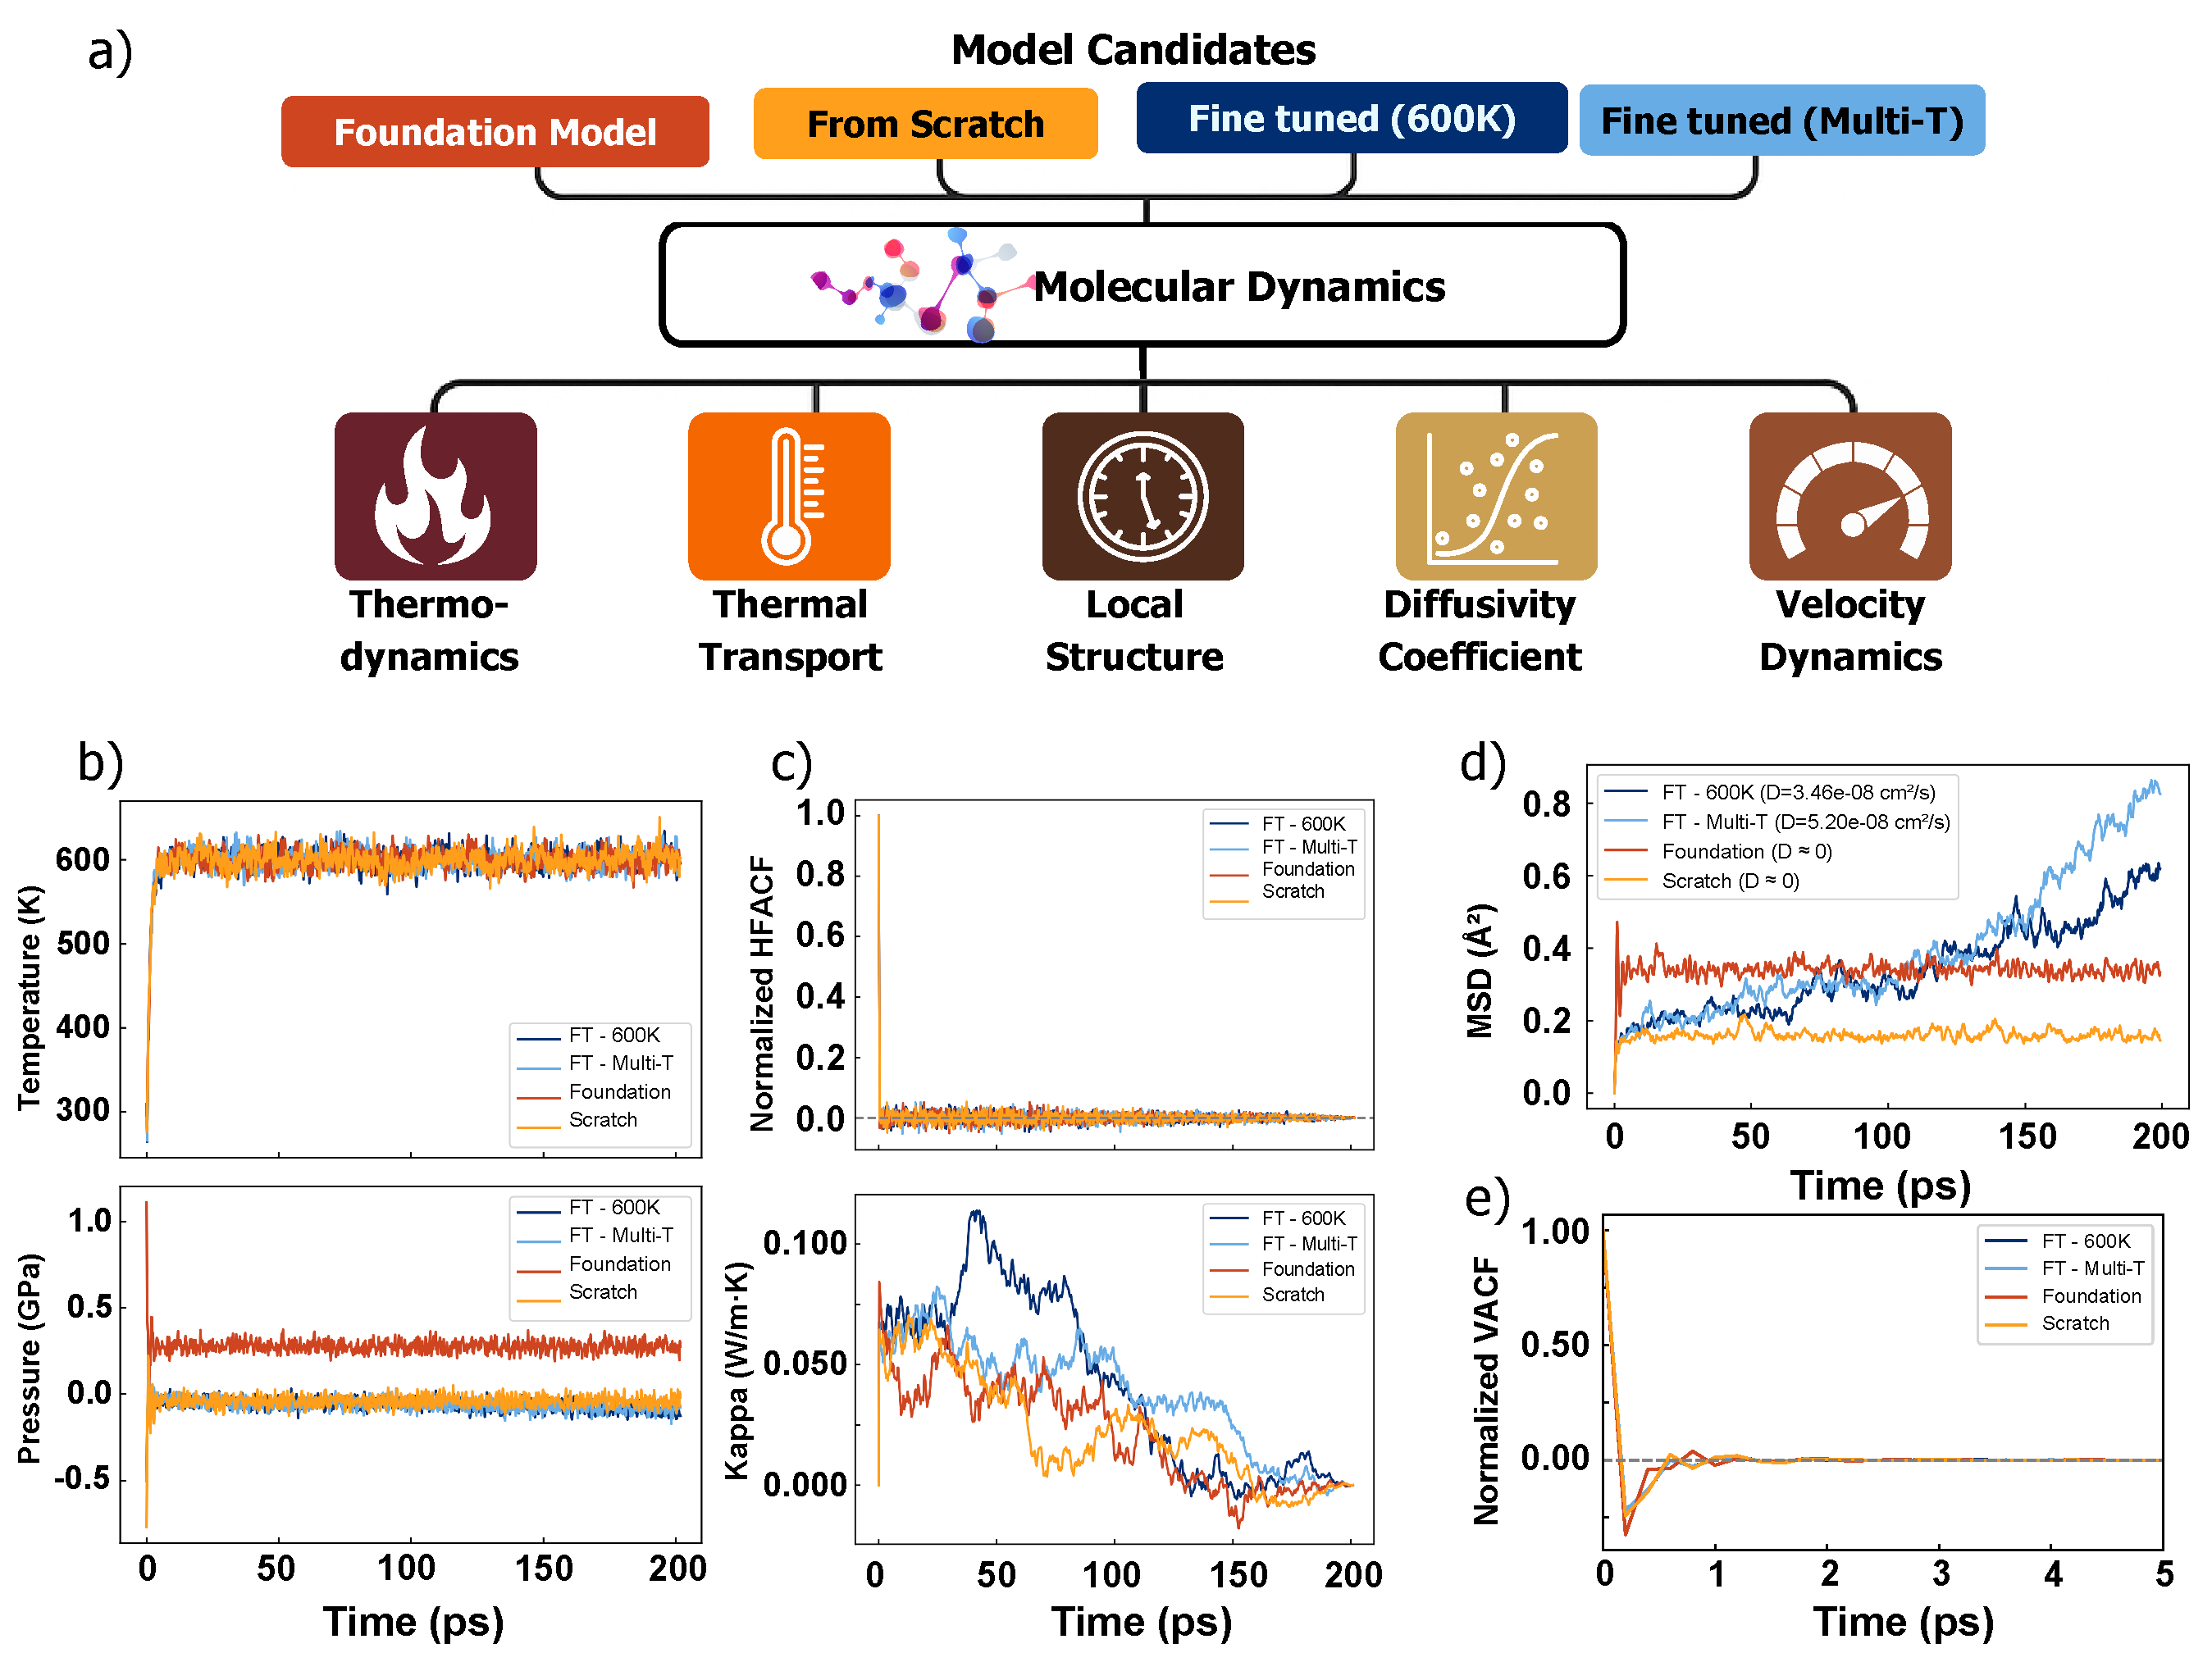
\includegraphics[width=\linewidth,height=0.42\textheight,keepaspectratio]{figure_pages/assets/fig_166.pdf}
\caption{Legacy published or conference-era benchmark figure retained for historical comparison. This page shows the candidate output ``Neurips2025 ai4mat fig2 v2'' within the audited LEGACY-NEURIPS family. The panel identity, source scope, and current status are retained in the accompanying evidence matrix.}
\label{fig:candidate_166}
\end{figure}
\textbf{Results text draft.} The figure is retained as an upstream reference asset. Its original protocol, data scope, and caption are not silently treated as identical to the Revision\textasciitilde{}1 audit.
\textbf{Discussion and boundary.} Use only when the manuscript explicitly labels the result as historical/upstream and states the protocol boundary.
\textbf{Article placement.} Proposed article location: Original main/SI manuscript.
\textbf{Reviewer linkage:} overall status NO\_DIRECT\_REVIEWER\_FIGURE\_LINK.
No direct reviewer-response figure linkage was identified; this page is retained for scientific/article audit rather than as a direct reviewer response.
\textbf{Evidence pointers.}
\begin{itemize}[leftmargin=1.4em,noitemsep]
\item Caption/text source: \begingroup\scriptsize\url{paper/paper/response_to_reviewers.log}\endgroup
\item Caption/text source: \begingroup\scriptsize\url{paper/paper/response_to_reviewers.out}\endgroup
\end{itemize}
\statusline{\textbf{Audit gap / next action:} Source-data and plotting provenance generally not co-located}
\vfill
\clearpage
\section{FIG-167 --- Neurips2025 ai4mat figure2}
\label{figpage:fig-167}
\textbf{Group:} LEGACY-NEURIPS\quad \textbf{Evidence chain:} partial\quad \textbf{Status:} publication
\begin{figure}[H]
\centering
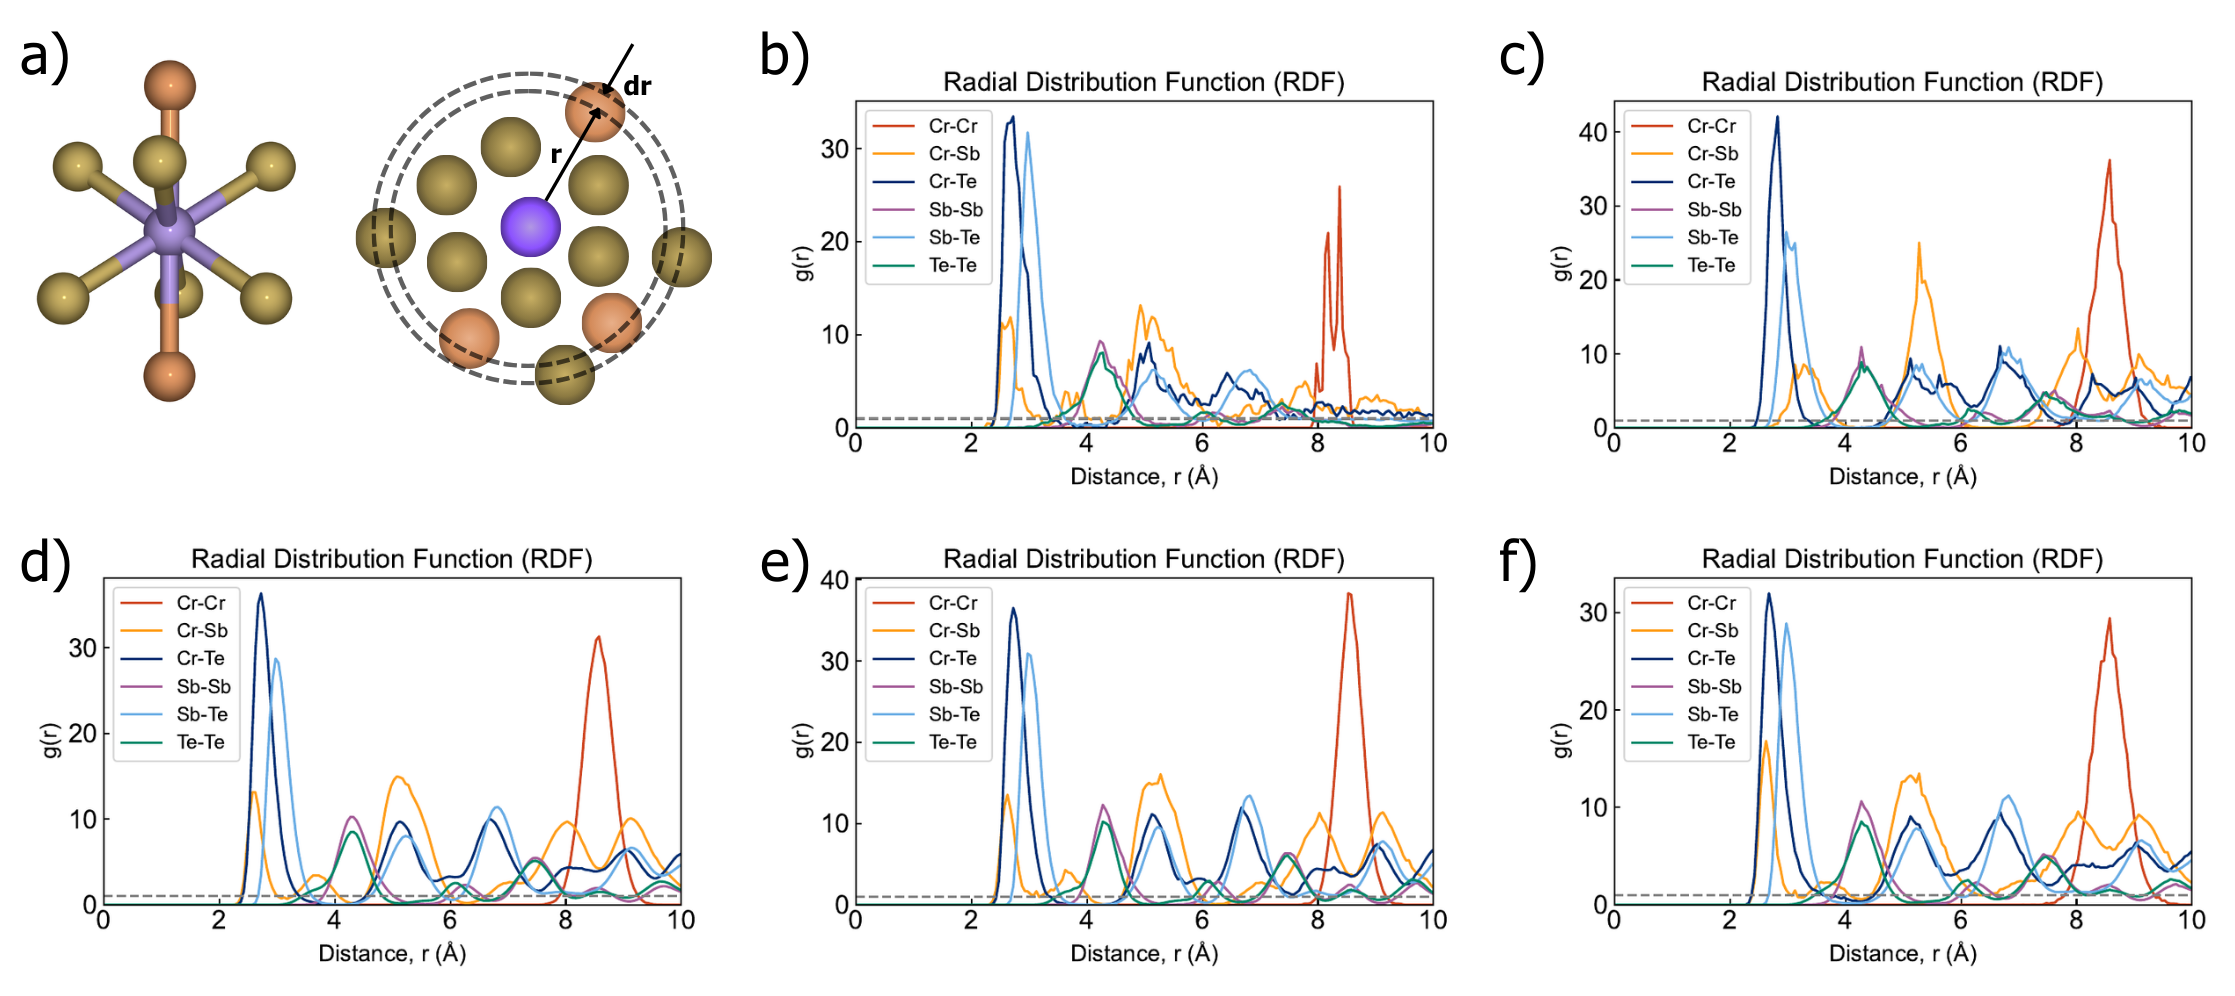
\includegraphics[width=\linewidth,height=0.42\textheight,keepaspectratio]{figure_pages/assets/fig_167.png}
\caption{Legacy published or conference-era benchmark figure retained for historical comparison. This page shows the candidate output ``Neurips2025 ai4mat figure2'' within the audited LEGACY-NEURIPS family. The panel identity, source scope, and current status are retained in the accompanying evidence matrix.}
\label{fig:candidate_167}
\end{figure}
\textbf{Results text draft.} The figure is retained as an upstream reference asset. Its original protocol, data scope, and caption are not silently treated as identical to the Revision\textasciitilde{}1 audit.
\textbf{Discussion and boundary.} Use only when the manuscript explicitly labels the result as historical/upstream and states the protocol boundary.
\textbf{Article placement.} Proposed article location: Original main/SI manuscript.
\textbf{Reviewer linkage:} overall status NO\_DIRECT\_REVIEWER\_FIGURE\_LINK.
No direct reviewer-response figure linkage was identified; this page is retained for scientific/article audit rather than as a direct reviewer response.
\textbf{Evidence pointers.}
\begin{itemize}[leftmargin=1.4em,noitemsep]
\item Caption/text source: \begingroup\scriptsize\url{paper/paper/response_to_reviewers.log}\endgroup
\item Caption/text source: \begingroup\scriptsize\url{paper/paper/response_to_reviewers.out}\endgroup
\end{itemize}
\statusline{\textbf{Audit gap / next action:} Source-data and plotting provenance generally not co-located}
\vfill
\clearpage
\section{FIG-168 --- Neurips2025 ai4mat figure3}
\label{figpage:fig-168}
\textbf{Group:} LEGACY-NEURIPS\quad \textbf{Evidence chain:} partial\quad \textbf{Status:} publication
\begin{figure}[H]
\centering
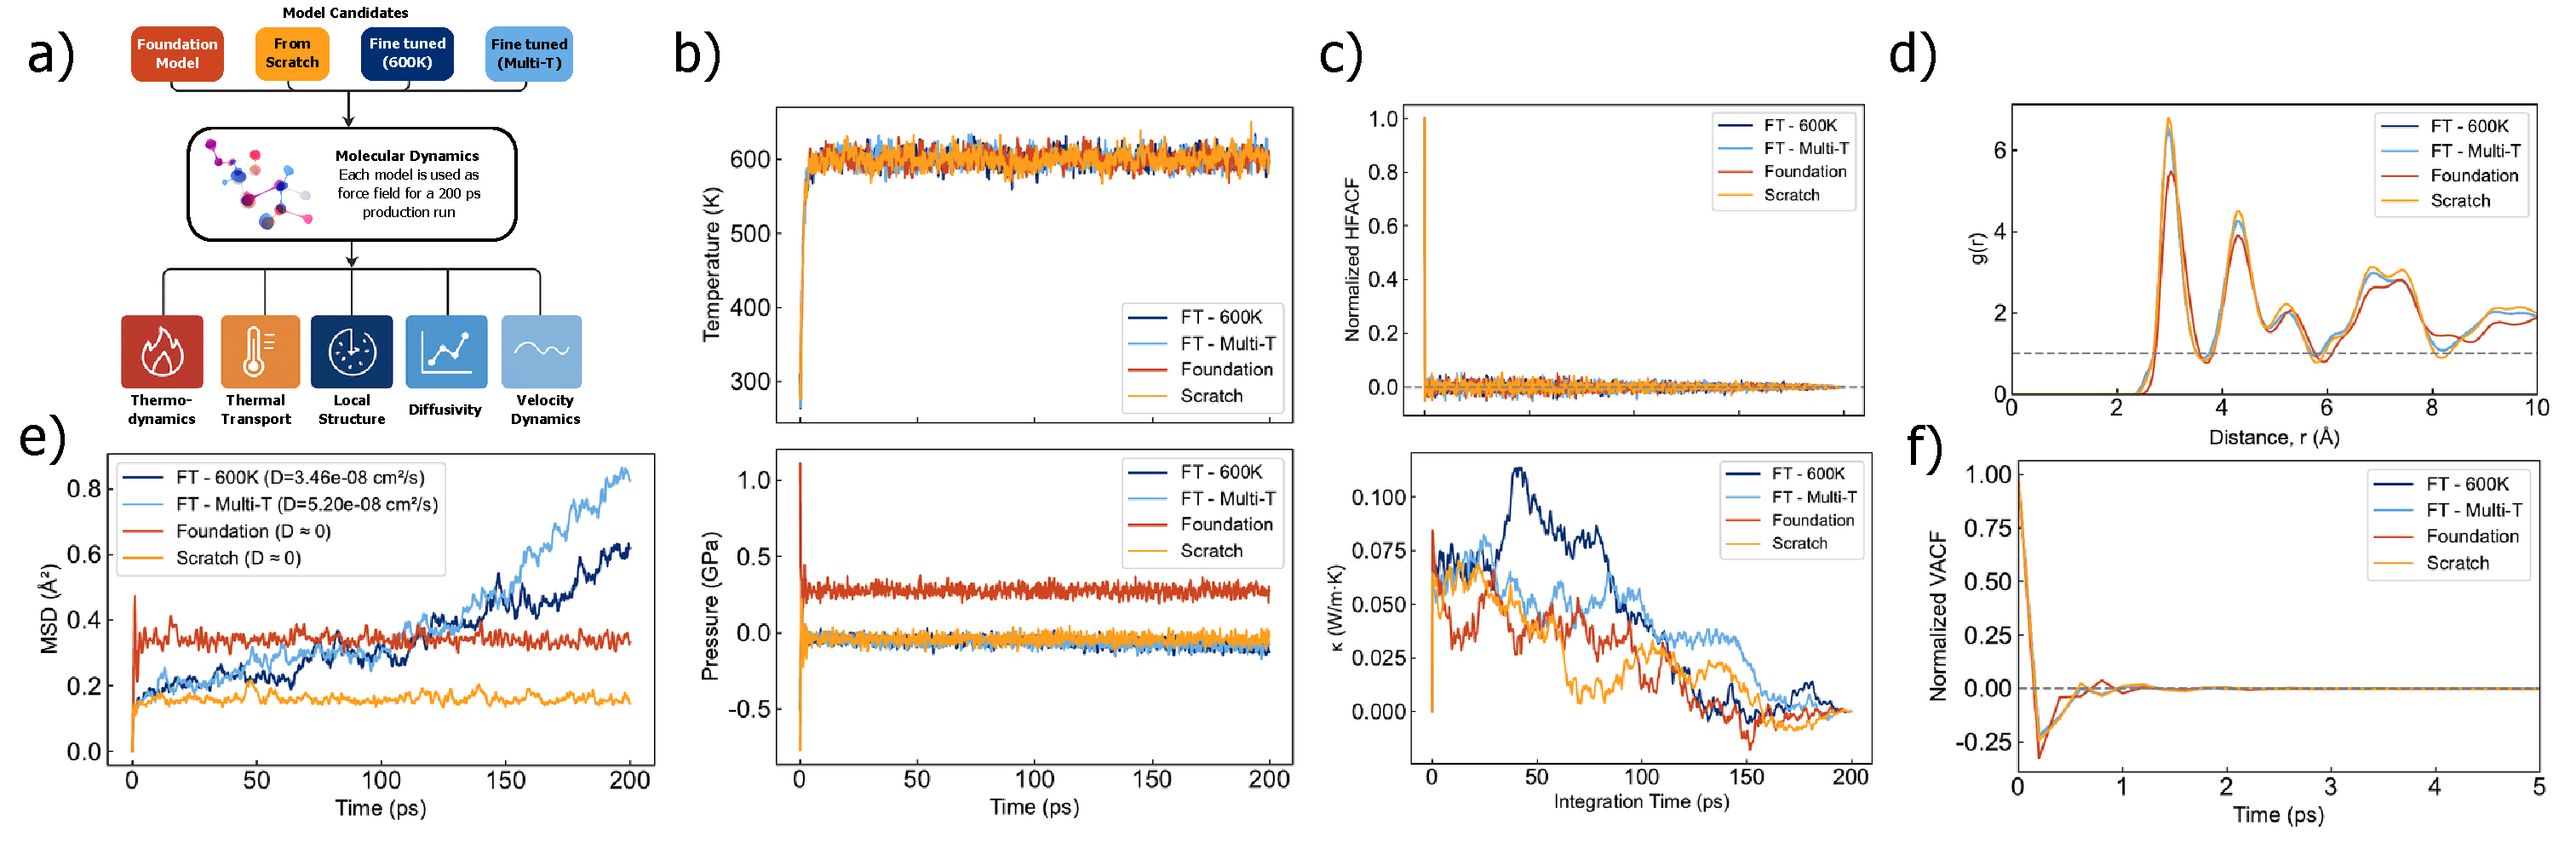
\includegraphics[width=\linewidth,height=0.42\textheight,keepaspectratio]{figure_pages/assets/fig_168.pdf}
\caption{Legacy published or conference-era benchmark figure retained for historical comparison. This page shows the candidate output ``Neurips2025 ai4mat figure3'' within the audited LEGACY-NEURIPS family. The panel identity, source scope, and current status are retained in the accompanying evidence matrix.}
\label{fig:candidate_168}
\end{figure}
\textbf{Results text draft.} The figure is retained as an upstream reference asset. Its original protocol, data scope, and caption are not silently treated as identical to the Revision\textasciitilde{}1 audit.
\textbf{Discussion and boundary.} Use only when the manuscript explicitly labels the result as historical/upstream and states the protocol boundary.
\textbf{Article placement.} Proposed article location: Original main/SI manuscript.
\textbf{Reviewer linkage:} overall status NO\_DIRECT\_REVIEWER\_FIGURE\_LINK.
No direct reviewer-response figure linkage was identified; this page is retained for scientific/article audit rather than as a direct reviewer response.
\textbf{Evidence pointers.}
\begin{itemize}[leftmargin=1.4em,noitemsep]
\item Caption/text source: \begingroup\scriptsize\url{paper/paper/response_to_reviewers.log}\endgroup
\item Caption/text source: \begingroup\scriptsize\url{paper/paper/response_to_reviewers.out}\endgroup
\end{itemize}
\statusline{\textbf{Audit gap / next action:} Source-data and plotting provenance generally not co-located}
\vfill
\clearpage
\section{FIG-169 --- Neurips2025 ai4mat figure4}
\label{figpage:fig-169}
\textbf{Group:} LEGACY-NEURIPS\quad \textbf{Evidence chain:} partial\quad \textbf{Status:} publication
\begin{figure}[H]
\centering
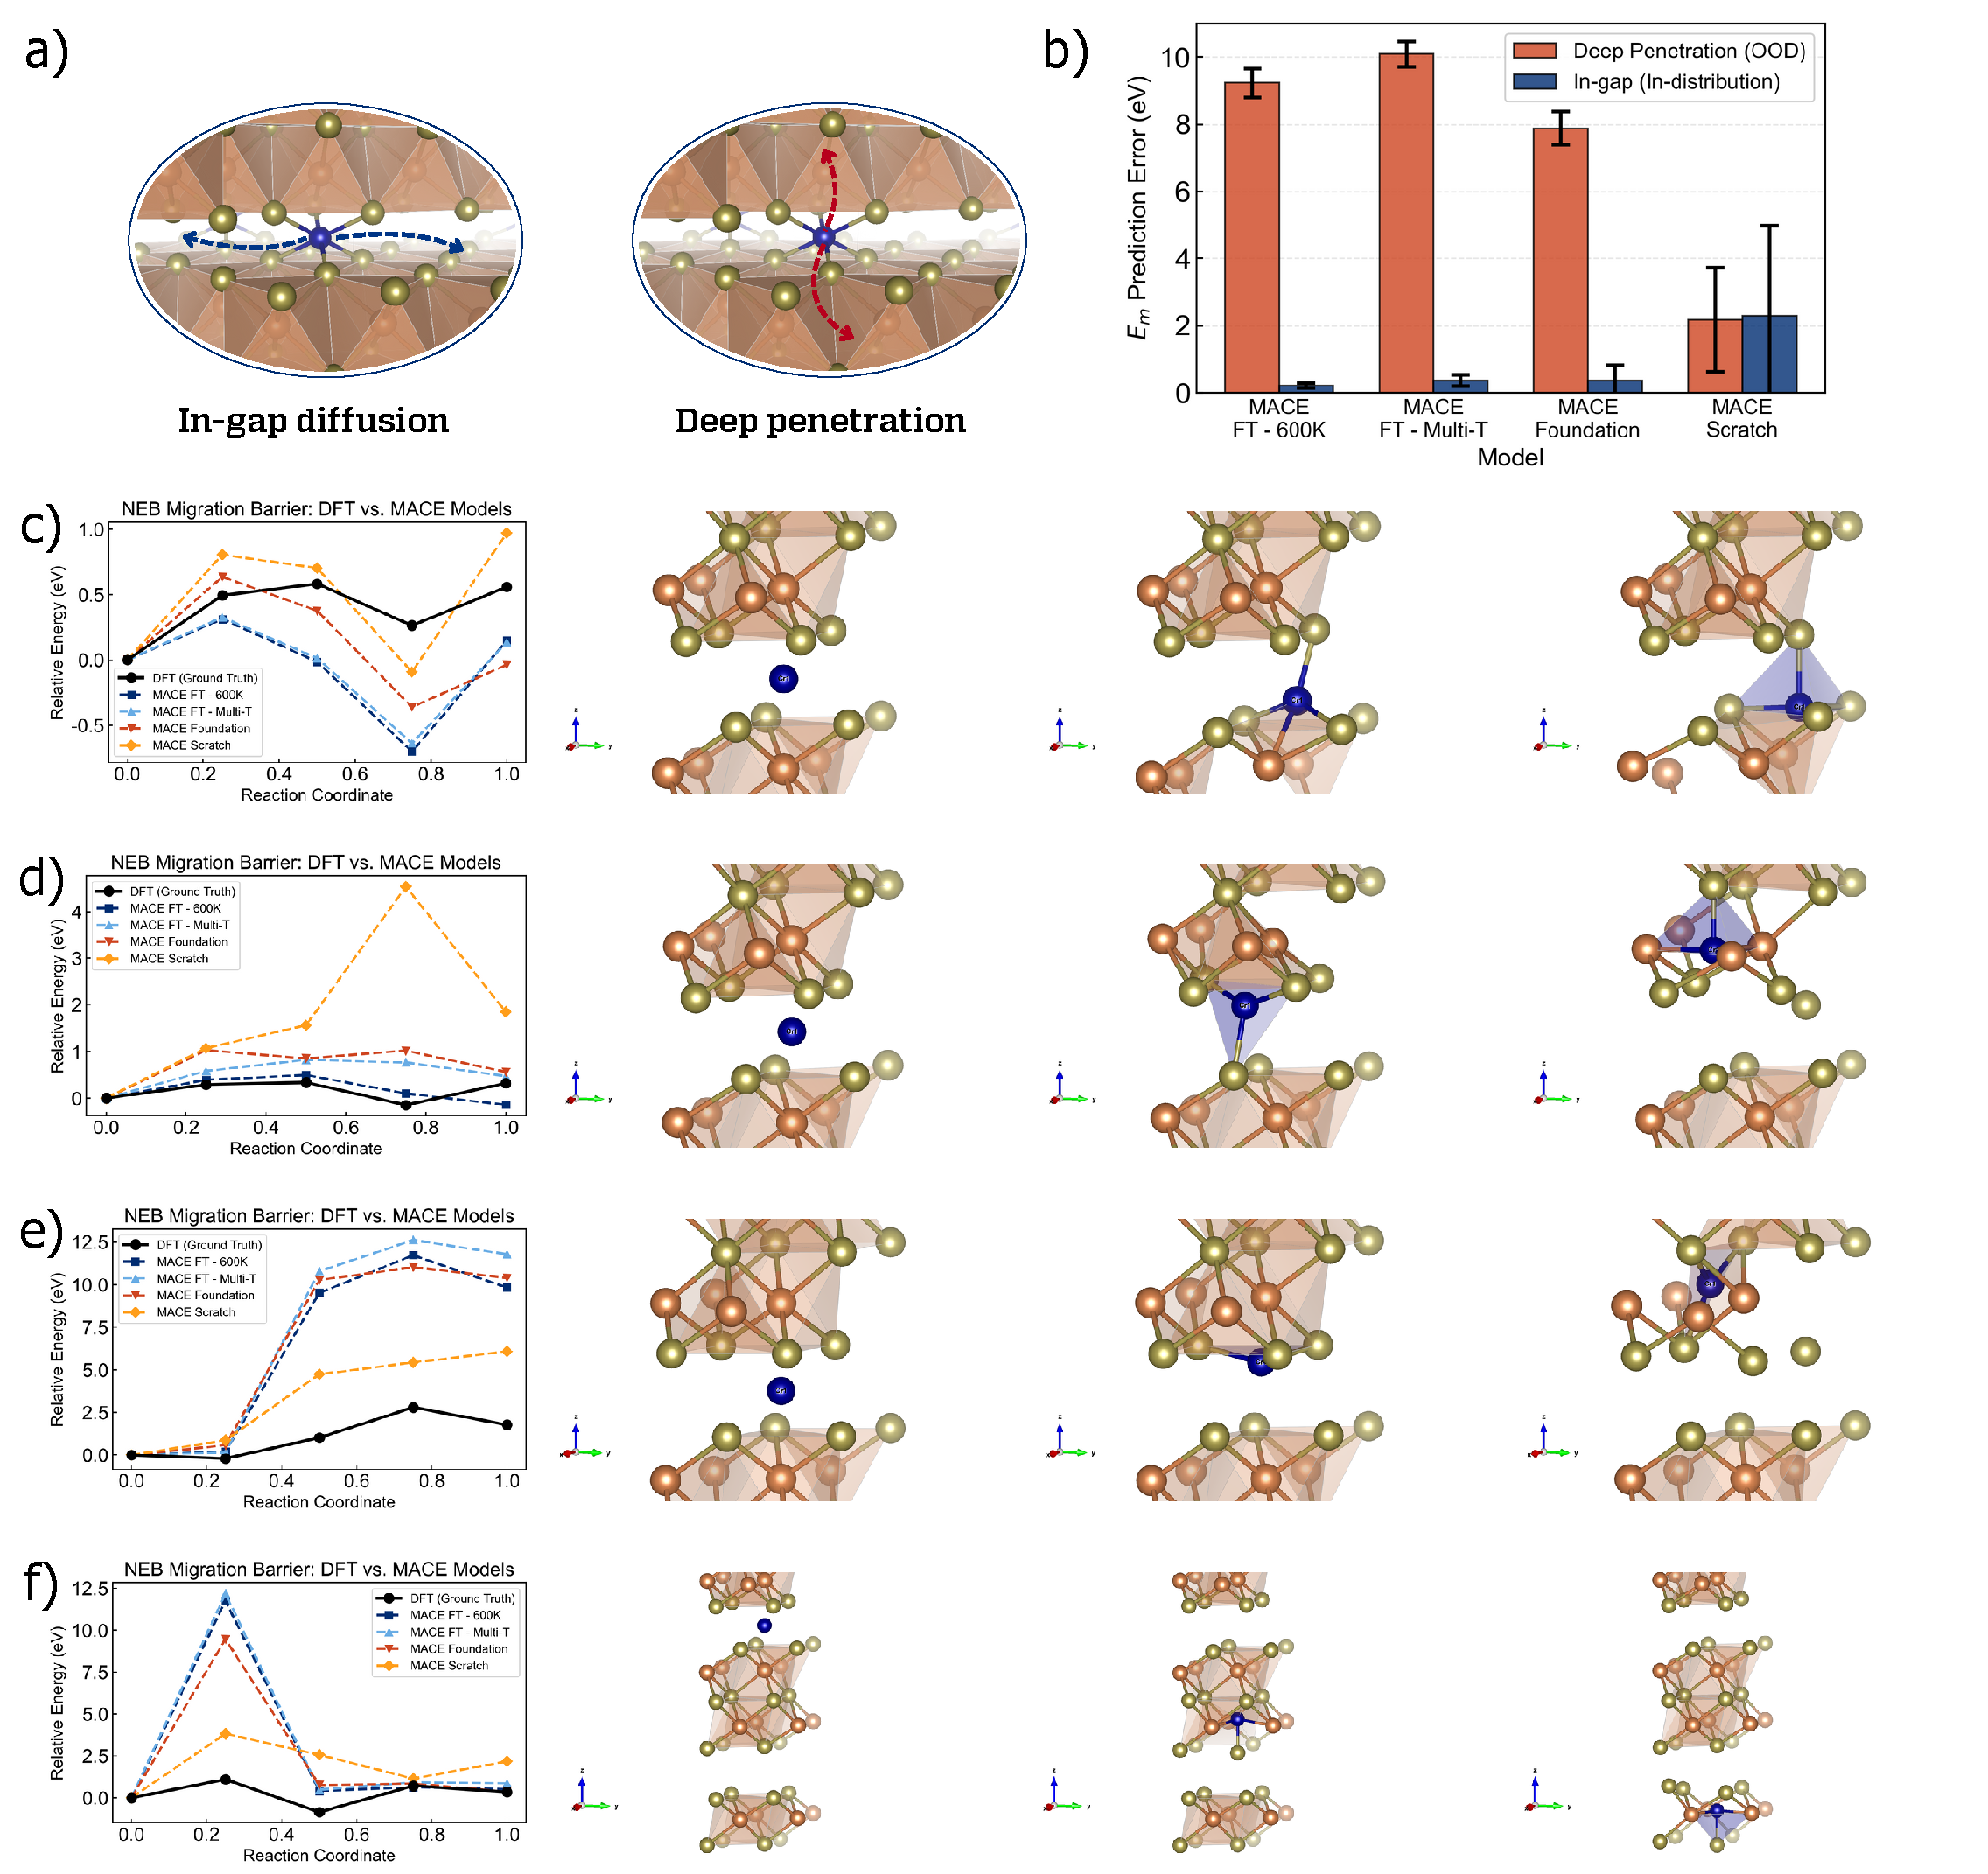
\includegraphics[width=\linewidth,height=0.42\textheight,keepaspectratio]{figure_pages/assets/fig_169.pdf}
\caption{Legacy published or conference-era benchmark figure retained for historical comparison. This page shows the candidate output ``Neurips2025 ai4mat figure4'' within the audited LEGACY-NEURIPS family. The panel identity, source scope, and current status are retained in the accompanying evidence matrix.}
\label{fig:candidate_169}
\end{figure}
\textbf{Results text draft.} The figure is retained as an upstream reference asset. Its original protocol, data scope, and caption are not silently treated as identical to the Revision\textasciitilde{}1 audit.
\textbf{Discussion and boundary.} Use only when the manuscript explicitly labels the result as historical/upstream and states the protocol boundary.
\textbf{Article placement.} Proposed article location: Original main/SI manuscript.
\textbf{Reviewer linkage:} overall status NO\_DIRECT\_REVIEWER\_FIGURE\_LINK.
No direct reviewer-response figure linkage was identified; this page is retained for scientific/article audit rather than as a direct reviewer response.
\textbf{Evidence pointers.}
\begin{itemize}[leftmargin=1.4em,noitemsep]
\item Caption/text source: \begingroup\scriptsize\url{paper/paper/response_to_reviewers.log}\endgroup
\item Caption/text source: \begingroup\scriptsize\url{paper/paper/response_to_reviewers.out}\endgroup
\end{itemize}
\statusline{\textbf{Audit gap / next action:} Source-data and plotting provenance generally not co-located}
\vfill
\clearpage
\section{FIG-170 --- Neurips2025 ai4mat figure4 v2}
\label{figpage:fig-170}
\textbf{Group:} LEGACY-NEURIPS\quad \textbf{Evidence chain:} partial\quad \textbf{Status:} publication
\begin{figure}[H]
\centering
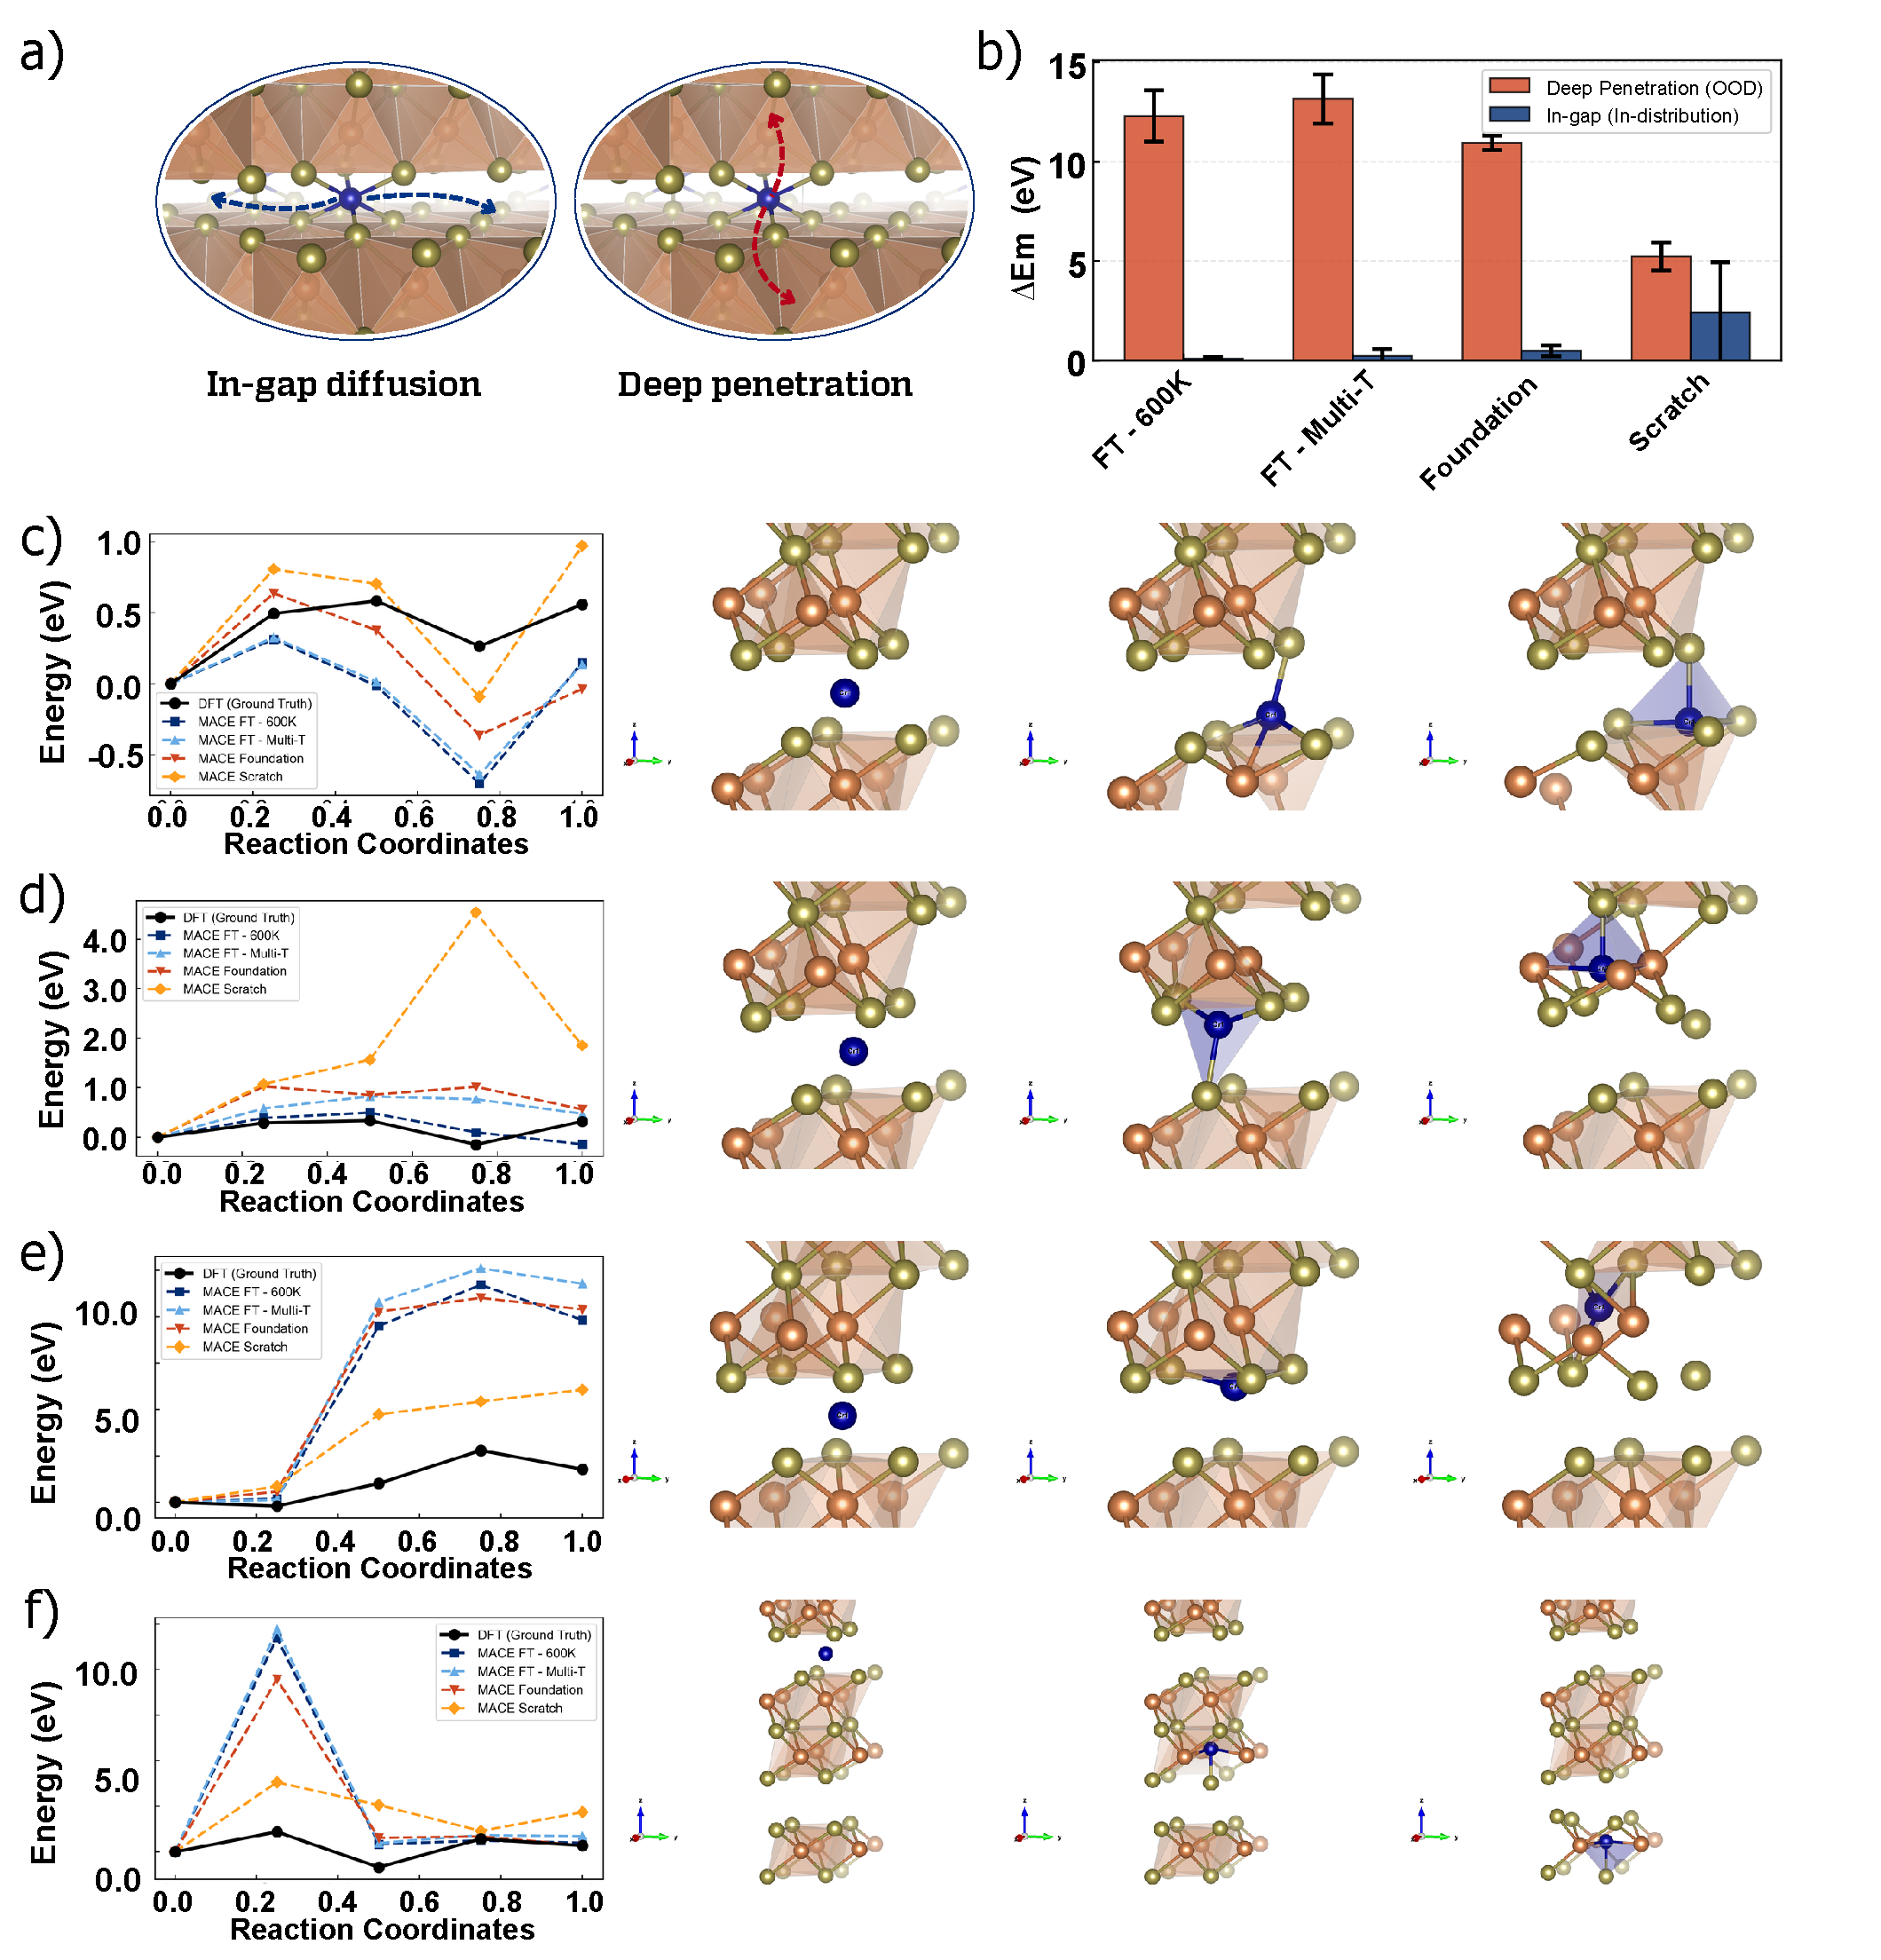
\includegraphics[width=\linewidth,height=0.42\textheight,keepaspectratio]{figure_pages/assets/fig_170.pdf}
\caption{Legacy published or conference-era benchmark figure retained for historical comparison. This page shows the candidate output ``Neurips2025 ai4mat figure4 v2'' within the audited LEGACY-NEURIPS family. The panel identity, source scope, and current status are retained in the accompanying evidence matrix.}
\label{fig:candidate_170}
\end{figure}
\textbf{Results text draft.} The figure is retained as an upstream reference asset. Its original protocol, data scope, and caption are not silently treated as identical to the Revision\textasciitilde{}1 audit.
\textbf{Discussion and boundary.} Use only when the manuscript explicitly labels the result as historical/upstream and states the protocol boundary.
\textbf{Article placement.} Proposed article location: Original main/SI manuscript.
\textbf{Reviewer linkage:} overall status NO\_DIRECT\_REVIEWER\_FIGURE\_LINK.
No direct reviewer-response figure linkage was identified; this page is retained for scientific/article audit rather than as a direct reviewer response.
\textbf{Evidence pointers.}
\begin{itemize}[leftmargin=1.4em,noitemsep]
\item Caption/text source: \begingroup\scriptsize\url{paper/paper/response_to_reviewers.log}\endgroup
\item Caption/text source: \begingroup\scriptsize\url{paper/paper/response_to_reviewers.out}\endgroup
\end{itemize}
\statusline{\textbf{Audit gap / next action:} Source-data and plotting provenance generally not co-located}
\vfill
\clearpage
\section{FIG-171 --- Neurips2025 ai4mat figure5}
\label{figpage:fig-171}
\textbf{Group:} LEGACY-NEURIPS\quad \textbf{Evidence chain:} partial\quad \textbf{Status:} publication
\begin{figure}[H]
\centering
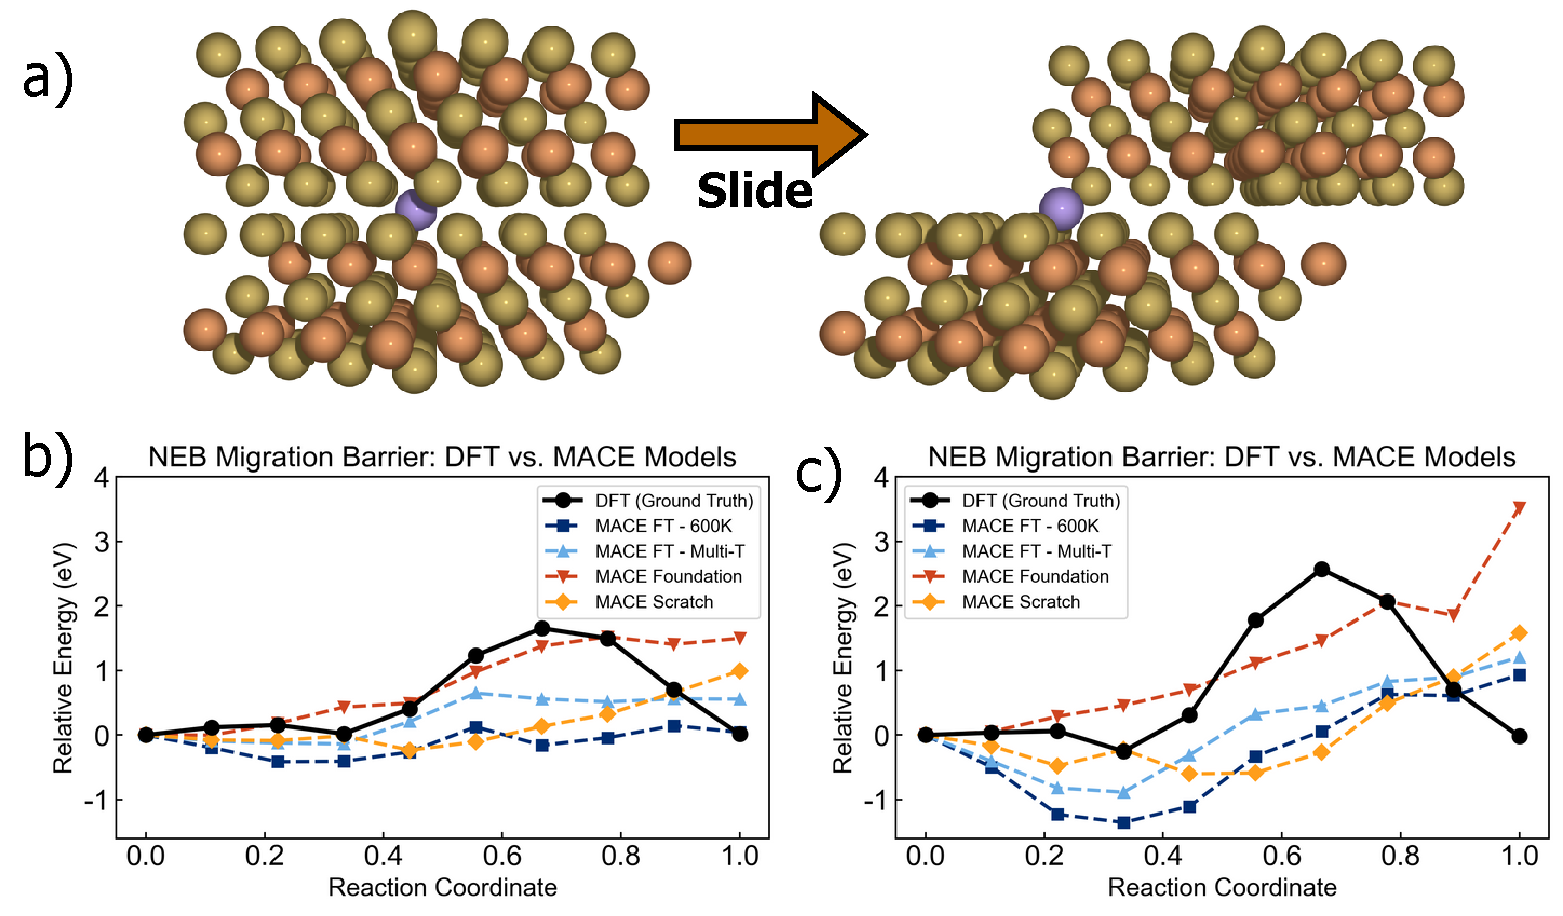
\includegraphics[width=\linewidth,height=0.42\textheight,keepaspectratio]{figure_pages/assets/fig_171.pdf}
\caption{Legacy published or conference-era benchmark figure retained for historical comparison. This page shows the candidate output ``Neurips2025 ai4mat figure5'' within the audited LEGACY-NEURIPS family. The panel identity, source scope, and current status are retained in the accompanying evidence matrix.}
\label{fig:candidate_171}
\end{figure}
\textbf{Results text draft.} The figure is retained as an upstream reference asset. Its original protocol, data scope, and caption are not silently treated as identical to the Revision\textasciitilde{}1 audit.
\textbf{Discussion and boundary.} Use only when the manuscript explicitly labels the result as historical/upstream and states the protocol boundary.
\textbf{Article placement.} Proposed article location: Original main/SI manuscript.
\textbf{Reviewer linkage:} overall status NO\_DIRECT\_REVIEWER\_FIGURE\_LINK.
No direct reviewer-response figure linkage was identified; this page is retained for scientific/article audit rather than as a direct reviewer response.
\textbf{Evidence pointers.}
\begin{itemize}[leftmargin=1.4em,noitemsep]
\item Caption/text source: \begingroup\scriptsize\url{paper/paper/response_to_reviewers.log}\endgroup
\item Caption/text source: \begingroup\scriptsize\url{paper/paper/response_to_reviewers.out}\endgroup
\end{itemize}
\statusline{\textbf{Audit gap / next action:} Source-data and plotting provenance generally not co-located}
\vfill
\clearpage
\section{FIG-172 --- Neurips2025 ai4mat figure6}
\label{figpage:fig-172}
\textbf{Group:} LEGACY-NEURIPS\quad \textbf{Evidence chain:} partial\quad \textbf{Status:} publication
\begin{figure}[H]
\centering
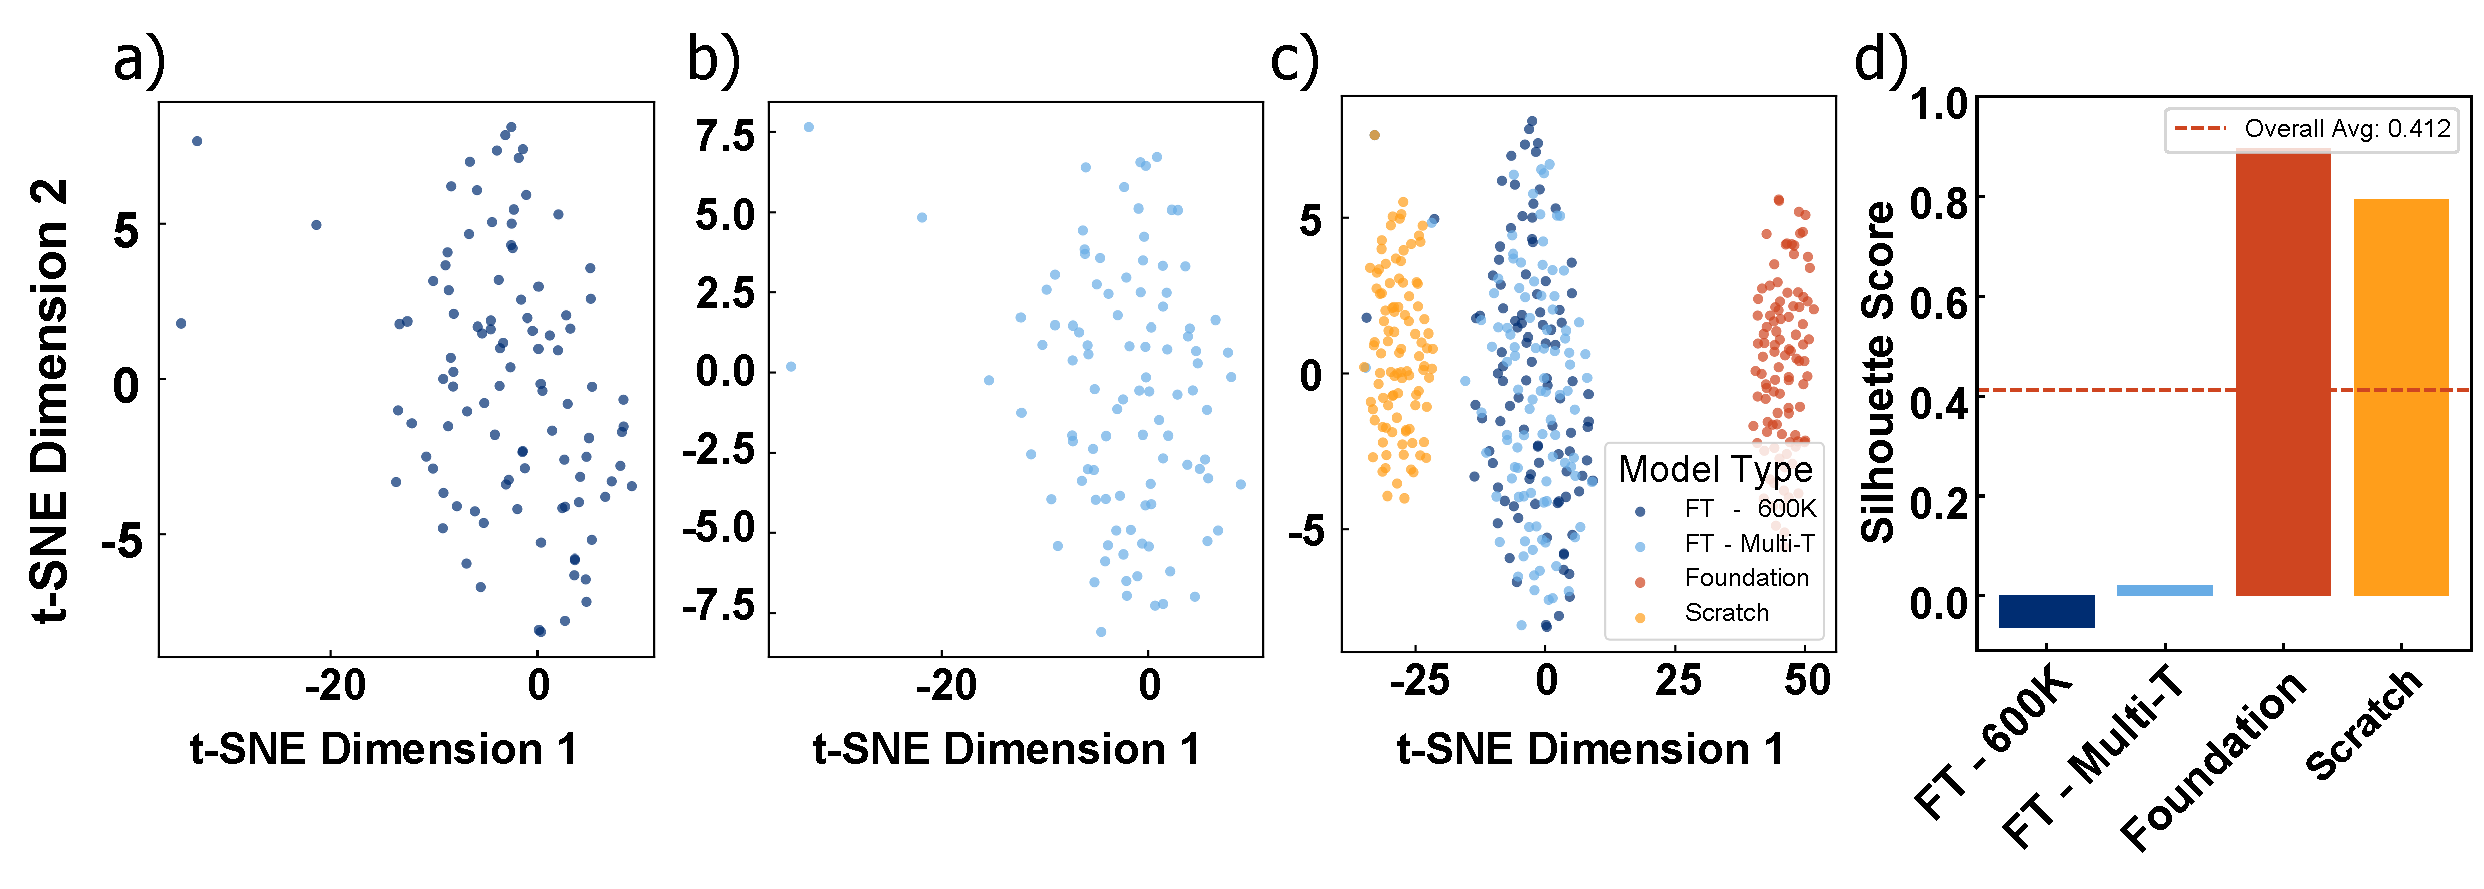
\includegraphics[width=\linewidth,height=0.42\textheight,keepaspectratio]{figure_pages/assets/fig_172.pdf}
\caption{Legacy published or conference-era benchmark figure retained for historical comparison. This page shows the candidate output ``Neurips2025 ai4mat figure6'' within the audited LEGACY-NEURIPS family. The panel identity, source scope, and current status are retained in the accompanying evidence matrix.}
\label{fig:candidate_172}
\end{figure}
\textbf{Results text draft.} The figure is retained as an upstream reference asset. Its original protocol, data scope, and caption are not silently treated as identical to the Revision\textasciitilde{}1 audit.
\textbf{Discussion and boundary.} Use only when the manuscript explicitly labels the result as historical/upstream and states the protocol boundary.
\textbf{Article placement.} Proposed article location: Original main/SI manuscript.
\textbf{Reviewer linkage:} overall status NO\_DIRECT\_REVIEWER\_FIGURE\_LINK.
No direct reviewer-response figure linkage was identified; this page is retained for scientific/article audit rather than as a direct reviewer response.
\textbf{Evidence pointers.}
\begin{itemize}[leftmargin=1.4em,noitemsep]
\item Caption/text source: \begingroup\scriptsize\url{paper/paper/response_to_reviewers.log}\endgroup
\item Caption/text source: \begingroup\scriptsize\url{paper/paper/response_to_reviewers.out}\endgroup
\end{itemize}
\statusline{\textbf{Audit gap / next action:} Source-data and plotting provenance generally not co-located}
\vfill
\clearpage
\section{FIG-173 --- Neurips2025 ai4mat figure6 phate}
\label{figpage:fig-173}
\textbf{Group:} LEGACY-NEURIPS\quad \textbf{Evidence chain:} partial\quad \textbf{Status:} publication
\begin{figure}[H]
\centering
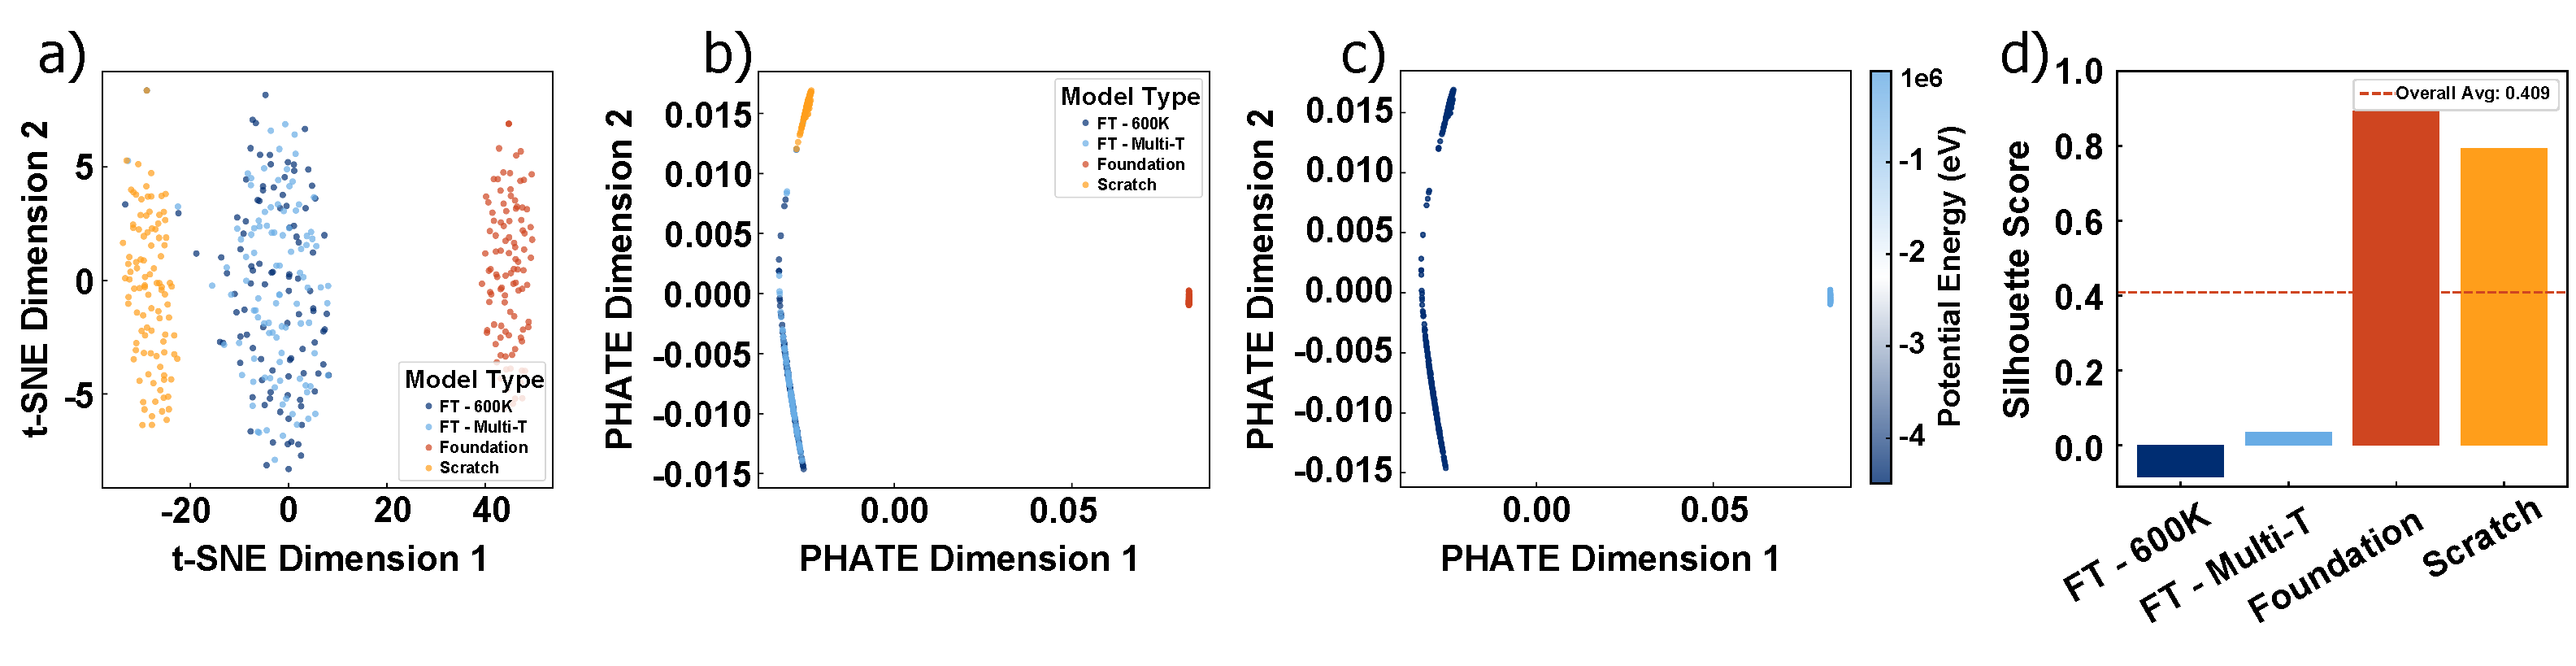
\includegraphics[width=\linewidth,height=0.42\textheight,keepaspectratio]{figure_pages/assets/fig_173.pdf}
\caption{Legacy published or conference-era benchmark figure retained for historical comparison. This page shows the candidate output ``Neurips2025 ai4mat figure6 phate'' within the audited LEGACY-NEURIPS family. The panel identity, source scope, and current status are retained in the accompanying evidence matrix.}
\label{fig:candidate_173}
\end{figure}
\textbf{Results text draft.} The figure is retained as an upstream reference asset. Its original protocol, data scope, and caption are not silently treated as identical to the Revision\textasciitilde{}1 audit.
\textbf{Discussion and boundary.} Use only when the manuscript explicitly labels the result as historical/upstream and states the protocol boundary.
\textbf{Article placement.} Proposed article location: Original main/SI manuscript.
\textbf{Reviewer linkage:} overall status PARTIAL.
\begin{itemize}[leftmargin=1.4em,noitemsep]
\item \textbf{REV-A6 (PARTIAL):} Soften t-SNE/PHATE and SHAP interpretation claims and add projection/original-space and surrogate-fidelity checks. \emph{Completed:} Projection sensitivity, original-descriptor-space separation, and per-model cross-validated surrogate R2 are available; the text is scoped to descriptive/surrogate evidence. \emph{Still required:} A direct MACE Cr-Cr perturbation test remains pending if a causal claim about the dominant feature is desired; otherwise retain the surrogate-scoped wording.
\item \textbf{REV-C11 (DONE):} Compute separability in the original/high-dimensional descriptor space rather than only on a 2D embedding. \emph{Completed:} Original-space metrics and projection-sensitivity checks are available; embedding scores are retained only as descriptive baselines. \emph{Still required:} No new numerical figure is required; preserve the feature-space definition and scaling sensitivity in the caption/methods.
\item \textbf{REV-C12 (DONE):} Remove the always-zero force-sensitivity feature stub from the latent analysis. \emph{Completed:} The inactive channel was removed and no unsupported force-sensitivity claim is made. \emph{Still required:} No additional figure evidence is required unless a genuine finite-difference force-sensitivity analysis is later added.
\end{itemize}
\textbf{Evidence pointers.}
\begin{itemize}[leftmargin=1.4em,noitemsep]
\item Caption/text source: \begingroup\scriptsize\url{paper/paper/response_to_reviewers.log}\endgroup
\item Caption/text source: \begingroup\scriptsize\url{paper/paper/response_to_reviewers.out}\endgroup
\end{itemize}
\statusline{\textbf{Audit gap / next action:} Source-data and plotting provenance generally not co-located}
\vfill
\clearpage
\section{FIG-174 --- Comparison error distribution}
\label{figpage:fig-174}
\textbf{Group:} LEGACY-SHAP\quad \textbf{Evidence chain:} partial\quad \textbf{Status:} publication;comparison
\begin{figure}[H]
\centering
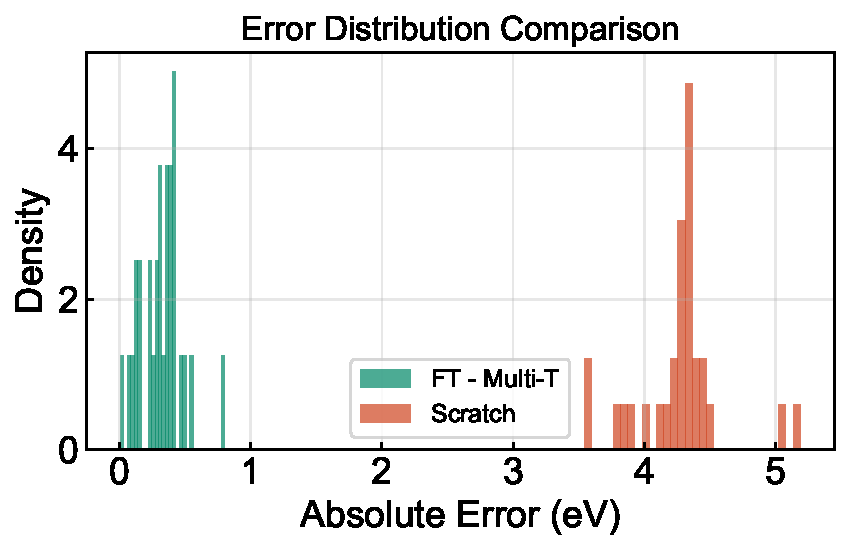
\includegraphics[width=\linewidth,height=0.42\textheight,keepaspectratio]{figure_pages/assets/fig_174.pdf}
\caption{Legacy shap or feature-attribution visualization. This page shows the candidate output ``Comparison error distribution'' within the audited LEGACY-SHAP family. The panel identity, source scope, and current status are retained in the accompanying evidence matrix.}
\label{fig:candidate_174}
\end{figure}
\textbf{Results text draft.} The figure displays the historical feature-attribution view and is kept separate from the corrected, frame-aligned surrogate analysis where applicable.
\textbf{Discussion and boundary.} Feature attribution is an interpretation diagnostic. It does not establish causal importance or transport/barrier accuracy without the declared surrogate-fidelity and perturbation checks.
\textbf{Article placement.} Proposed article location: Legacy Fig. 6/interpretability audit.
\textbf{Reviewer linkage:} overall status PARTIAL.
\begin{itemize}[leftmargin=1.4em,noitemsep]
\item \textbf{REV-A6 (PARTIAL):} Soften t-SNE/PHATE and SHAP interpretation claims and add projection/original-space and surrogate-fidelity checks. \emph{Completed:} Projection sensitivity, original-descriptor-space separation, and per-model cross-validated surrogate R2 are available; the text is scoped to descriptive/surrogate evidence. \emph{Still required:} A direct MACE Cr-Cr perturbation test remains pending if a causal claim about the dominant feature is desired; otherwise retain the surrogate-scoped wording.
\item \textbf{REV-C13 (PARTIAL):} Make the SHAP pipeline and advertised repository artifacts reproducible rather than leaving empty stubs. \emph{Completed:} The corrected SHAP inputs, scripts, lineage, and locked revised outputs are present for the declared three-model/150-frame scope. \emph{Still required:} Close the final release/empty-stub audit and reconcile the independent rerun with the locked historical CSV before claiming exact end-to-end regeneration.
\end{itemize}
\textbf{Evidence pointers.}
No data/script/text candidate was recorded in the matrix; resolve this gap before manuscript promotion.
\statusline{\textbf{Audit gap / next action:} Some images lack direct source-data and renderer linkage}
\vfill
\clearpage
\section{FIG-175 --- Comparison feature stability}
\label{figpage:fig-175}
\textbf{Group:} LEGACY-SHAP\quad \textbf{Evidence chain:} partial\quad \textbf{Status:} publication;comparison
\begin{figure}[H]
\centering
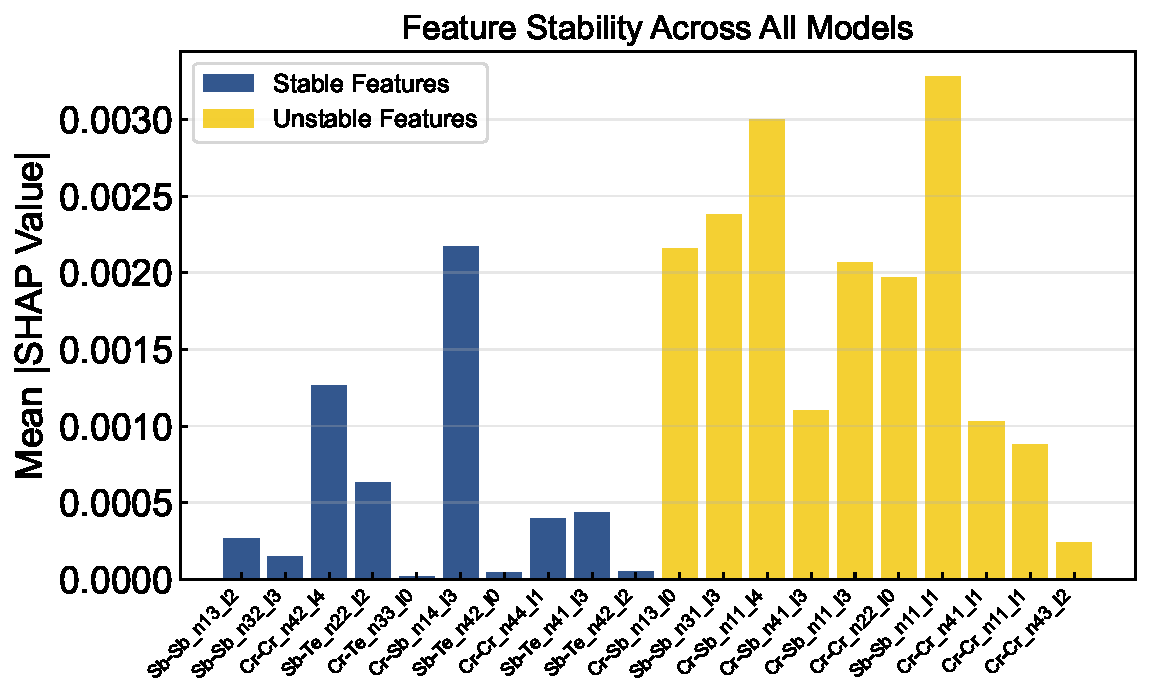
\includegraphics[width=\linewidth,height=0.42\textheight,keepaspectratio]{figure_pages/assets/fig_175.pdf}
\caption{Legacy shap or feature-attribution visualization. This page shows the candidate output ``Comparison feature stability'' within the audited LEGACY-SHAP family. The panel identity, source scope, and current status are retained in the accompanying evidence matrix.}
\label{fig:candidate_175}
\end{figure}
\textbf{Results text draft.} The figure displays the historical feature-attribution view and is kept separate from the corrected, frame-aligned surrogate analysis where applicable.
\textbf{Discussion and boundary.} Feature attribution is an interpretation diagnostic. It does not establish causal importance or transport/barrier accuracy without the declared surrogate-fidelity and perturbation checks.
\textbf{Article placement.} Proposed article location: Legacy Fig. 6/interpretability audit.
\textbf{Reviewer linkage:} overall status PARTIAL.
\begin{itemize}[leftmargin=1.4em,noitemsep]
\item \textbf{REV-A6 (PARTIAL):} Soften t-SNE/PHATE and SHAP interpretation claims and add projection/original-space and surrogate-fidelity checks. \emph{Completed:} Projection sensitivity, original-descriptor-space separation, and per-model cross-validated surrogate R2 are available; the text is scoped to descriptive/surrogate evidence. \emph{Still required:} A direct MACE Cr-Cr perturbation test remains pending if a causal claim about the dominant feature is desired; otherwise retain the surrogate-scoped wording.
\item \textbf{REV-C13 (PARTIAL):} Make the SHAP pipeline and advertised repository artifacts reproducible rather than leaving empty stubs. \emph{Completed:} The corrected SHAP inputs, scripts, lineage, and locked revised outputs are present for the declared three-model/150-frame scope. \emph{Still required:} Close the final release/empty-stub audit and reconcile the independent rerun with the locked historical CSV before claiming exact end-to-end regeneration.
\end{itemize}
\textbf{Evidence pointers.}
No data/script/text candidate was recorded in the matrix; resolve this gap before manuscript promotion.
\statusline{\textbf{Audit gap / next action:} Some images lack direct source-data and renderer linkage}
\vfill
\clearpage
\section{FIG-176 --- Comparison prediction scatter}
\label{figpage:fig-176}
\textbf{Group:} LEGACY-SHAP\quad \textbf{Evidence chain:} partial\quad \textbf{Status:} publication;comparison
\begin{figure}[H]
\centering
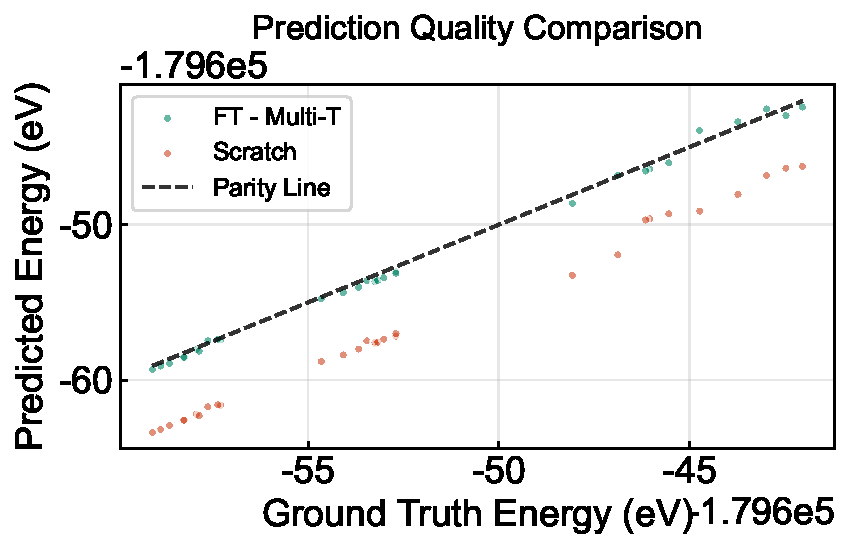
\includegraphics[width=\linewidth,height=0.42\textheight,keepaspectratio]{figure_pages/assets/fig_176.pdf}
\caption{Legacy shap or feature-attribution visualization. This page shows the candidate output ``Comparison prediction scatter'' within the audited LEGACY-SHAP family. The panel identity, source scope, and current status are retained in the accompanying evidence matrix.}
\label{fig:candidate_176}
\end{figure}
\textbf{Results text draft.} The figure displays the historical feature-attribution view and is kept separate from the corrected, frame-aligned surrogate analysis where applicable.
\textbf{Discussion and boundary.} Feature attribution is an interpretation diagnostic. It does not establish causal importance or transport/barrier accuracy without the declared surrogate-fidelity and perturbation checks.
\textbf{Article placement.} Proposed article location: Legacy Fig. 6/interpretability audit.
\textbf{Reviewer linkage:} overall status PARTIAL.
\begin{itemize}[leftmargin=1.4em,noitemsep]
\item \textbf{REV-A6 (PARTIAL):} Soften t-SNE/PHATE and SHAP interpretation claims and add projection/original-space and surrogate-fidelity checks. \emph{Completed:} Projection sensitivity, original-descriptor-space separation, and per-model cross-validated surrogate R2 are available; the text is scoped to descriptive/surrogate evidence. \emph{Still required:} A direct MACE Cr-Cr perturbation test remains pending if a causal claim about the dominant feature is desired; otherwise retain the surrogate-scoped wording.
\item \textbf{REV-C13 (PARTIAL):} Make the SHAP pipeline and advertised repository artifacts reproducible rather than leaving empty stubs. \emph{Completed:} The corrected SHAP inputs, scripts, lineage, and locked revised outputs are present for the declared three-model/150-frame scope. \emph{Still required:} Close the final release/empty-stub audit and reconcile the independent rerun with the locked historical CSV before claiming exact end-to-end regeneration.
\end{itemize}
\textbf{Evidence pointers.}
No data/script/text candidate was recorded in the matrix; resolve this gap before manuscript promotion.
\statusline{\textbf{Audit gap / next action:} Some images lack direct source-data and renderer linkage}
\vfill
\clearpage
\section{FIG-177 --- Comparison top15 difference}
\label{figpage:fig-177}
\textbf{Group:} LEGACY-SHAP\quad \textbf{Evidence chain:} partial\quad \textbf{Status:} publication;comparison
\begin{figure}[H]
\centering
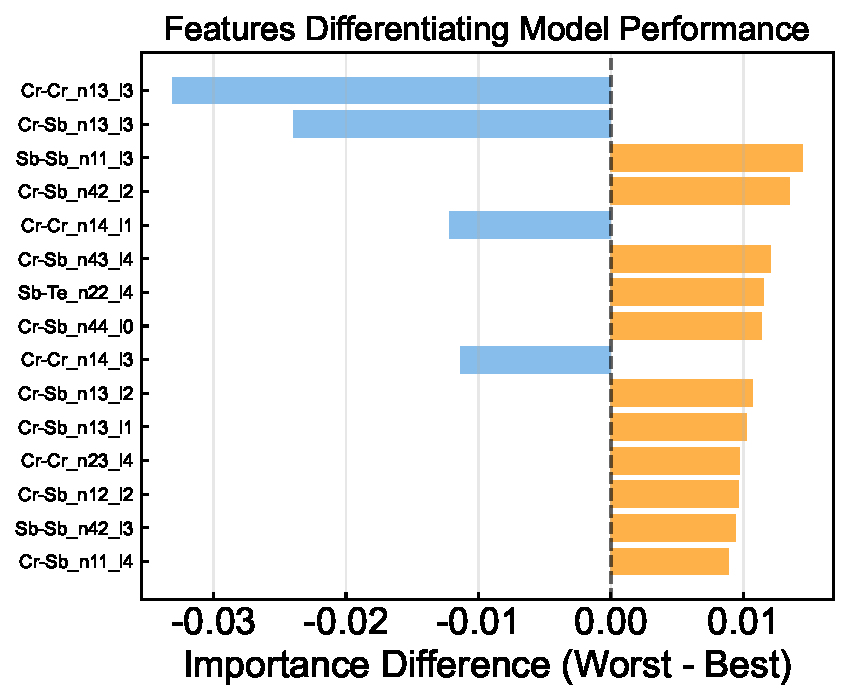
\includegraphics[width=\linewidth,height=0.42\textheight,keepaspectratio]{figure_pages/assets/fig_177.pdf}
\caption{Legacy shap or feature-attribution visualization. This page shows the candidate output ``Comparison top15 difference'' within the audited LEGACY-SHAP family. The panel identity, source scope, and current status are retained in the accompanying evidence matrix.}
\label{fig:candidate_177}
\end{figure}
\textbf{Results text draft.} The figure displays the historical feature-attribution view and is kept separate from the corrected, frame-aligned surrogate analysis where applicable.
\textbf{Discussion and boundary.} Feature attribution is an interpretation diagnostic. It does not establish causal importance or transport/barrier accuracy without the declared surrogate-fidelity and perturbation checks.
\textbf{Article placement.} Proposed article location: Legacy Fig. 6/interpretability audit.
\textbf{Reviewer linkage:} overall status PARTIAL.
\begin{itemize}[leftmargin=1.4em,noitemsep]
\item \textbf{REV-A6 (PARTIAL):} Soften t-SNE/PHATE and SHAP interpretation claims and add projection/original-space and surrogate-fidelity checks. \emph{Completed:} Projection sensitivity, original-descriptor-space separation, and per-model cross-validated surrogate R2 are available; the text is scoped to descriptive/surrogate evidence. \emph{Still required:} A direct MACE Cr-Cr perturbation test remains pending if a causal claim about the dominant feature is desired; otherwise retain the surrogate-scoped wording.
\item \textbf{REV-C13 (PARTIAL):} Make the SHAP pipeline and advertised repository artifacts reproducible rather than leaving empty stubs. \emph{Completed:} The corrected SHAP inputs, scripts, lineage, and locked revised outputs are present for the declared three-model/150-frame scope. \emph{Still required:} Close the final release/empty-stub audit and reconcile the independent rerun with the locked historical CSV before claiming exact end-to-end regeneration.
\end{itemize}
\textbf{Evidence pointers.}
No data/script/text candidate was recorded in the matrix; resolve this gap before manuscript promotion.
\statusline{\textbf{Audit gap / next action:} Some images lack direct source-data and renderer linkage}
\vfill
\clearpage
\section{FIG-178 --- Comparison top50 difference}
\label{figpage:fig-178}
\textbf{Group:} LEGACY-SHAP\quad \textbf{Evidence chain:} partial\quad \textbf{Status:} publication;comparison
\begin{figure}[H]
\centering
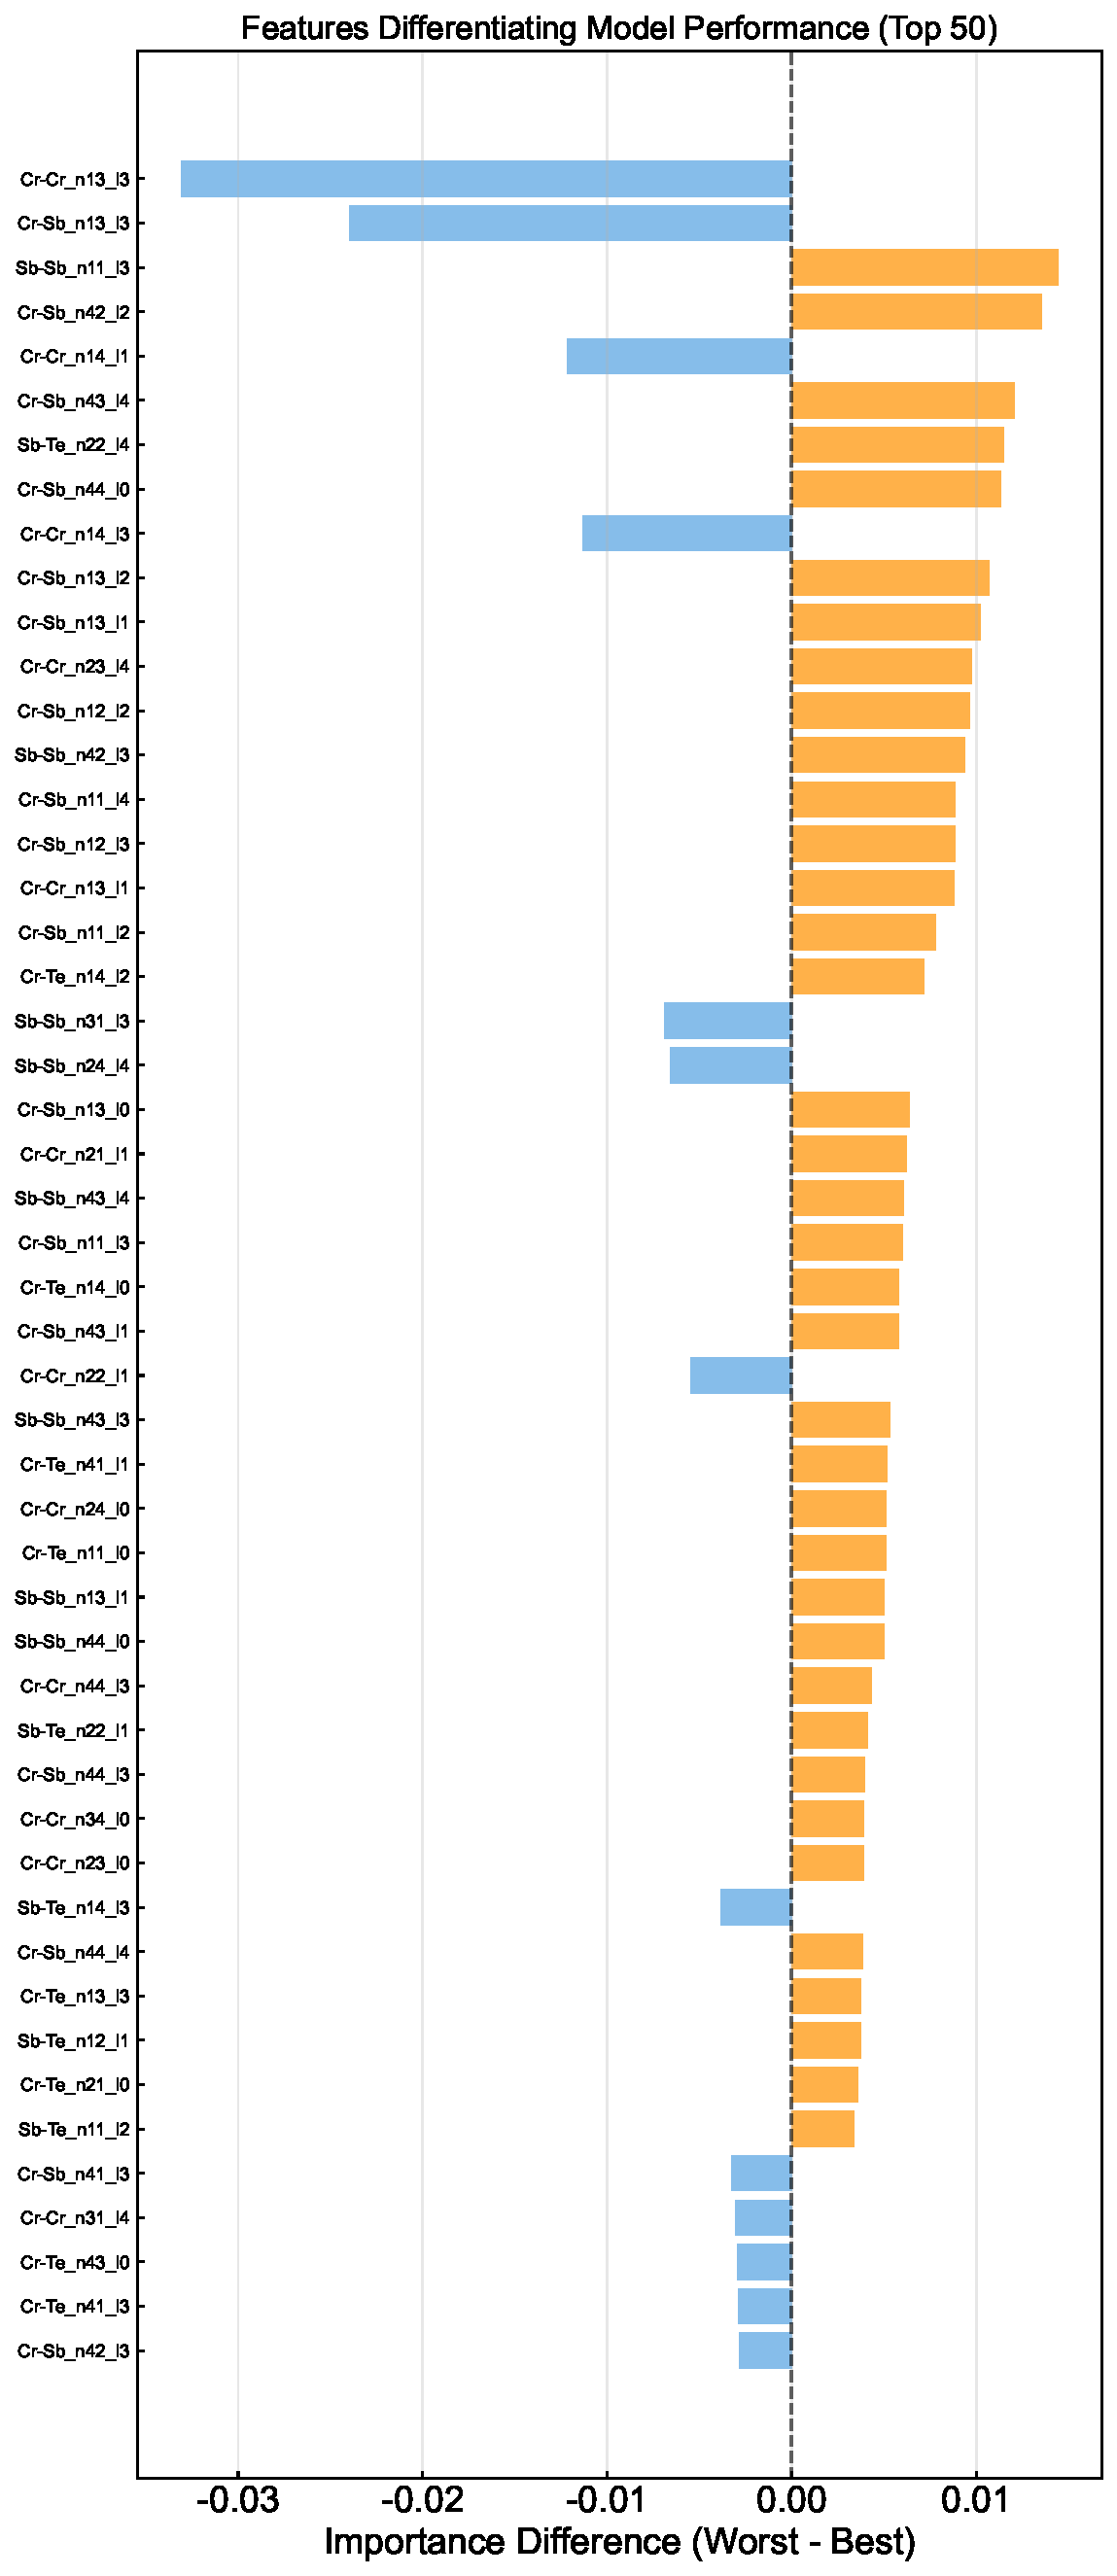
\includegraphics[width=\linewidth,height=0.42\textheight,keepaspectratio]{figure_pages/assets/fig_178.pdf}
\caption{Legacy shap or feature-attribution visualization. This page shows the candidate output ``Comparison top50 difference'' within the audited LEGACY-SHAP family. The panel identity, source scope, and current status are retained in the accompanying evidence matrix.}
\label{fig:candidate_178}
\end{figure}
\textbf{Results text draft.} The figure displays the historical feature-attribution view and is kept separate from the corrected, frame-aligned surrogate analysis where applicable.
\textbf{Discussion and boundary.} Feature attribution is an interpretation diagnostic. It does not establish causal importance or transport/barrier accuracy without the declared surrogate-fidelity and perturbation checks.
\textbf{Article placement.} Proposed article location: Legacy Fig. 6/interpretability audit.
\textbf{Reviewer linkage:} overall status PARTIAL.
\begin{itemize}[leftmargin=1.4em,noitemsep]
\item \textbf{REV-A6 (PARTIAL):} Soften t-SNE/PHATE and SHAP interpretation claims and add projection/original-space and surrogate-fidelity checks. \emph{Completed:} Projection sensitivity, original-descriptor-space separation, and per-model cross-validated surrogate R2 are available; the text is scoped to descriptive/surrogate evidence. \emph{Still required:} A direct MACE Cr-Cr perturbation test remains pending if a causal claim about the dominant feature is desired; otherwise retain the surrogate-scoped wording.
\item \textbf{REV-C13 (PARTIAL):} Make the SHAP pipeline and advertised repository artifacts reproducible rather than leaving empty stubs. \emph{Completed:} The corrected SHAP inputs, scripts, lineage, and locked revised outputs are present for the declared three-model/150-frame scope. \emph{Still required:} Close the final release/empty-stub audit and reconcile the independent rerun with the locked historical CSV before claiming exact end-to-end regeneration.
\end{itemize}
\textbf{Evidence pointers.}
No data/script/text candidate was recorded in the matrix; resolve this gap before manuscript promotion.
\statusline{\textbf{Audit gap / next action:} Some images lack direct source-data and renderer linkage}
\vfill
\clearpage
\section{FIG-179 --- Enhanced error feature analysis}
\label{figpage:fig-179}
\textbf{Group:} LEGACY-SHAP\quad \textbf{Evidence chain:} partial\quad \textbf{Status:} publication
\begin{figure}[H]
\centering
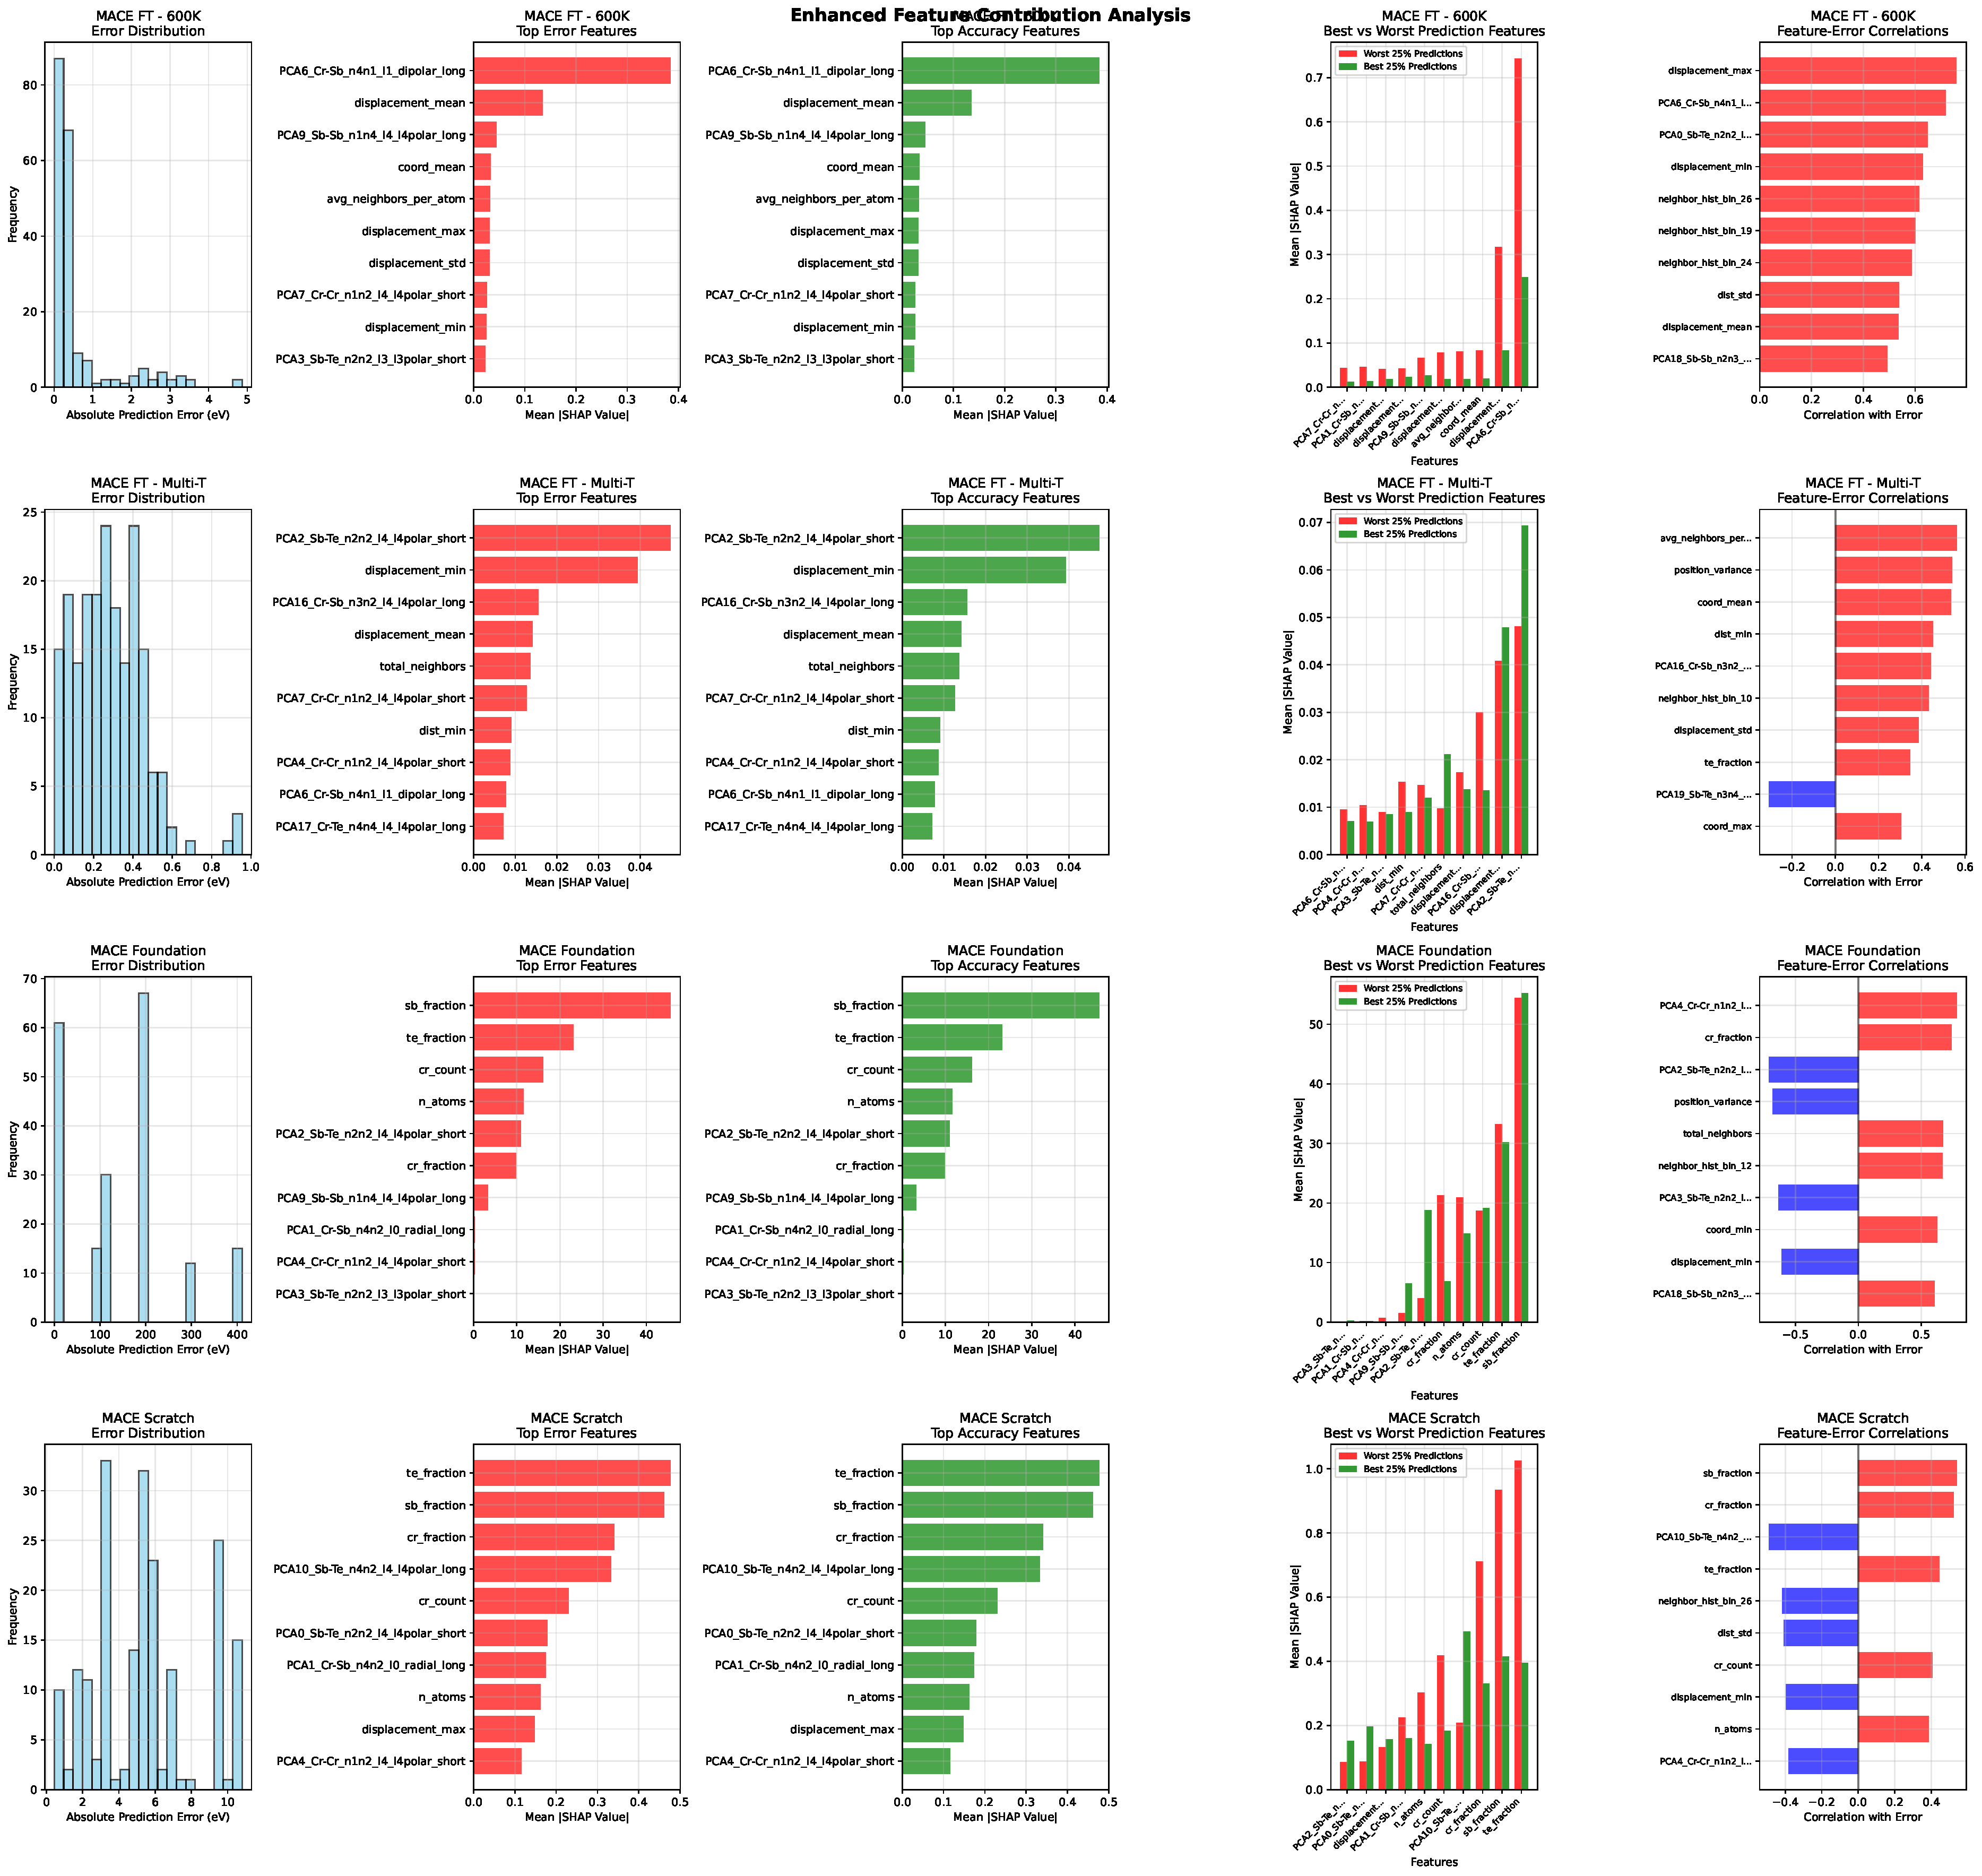
\includegraphics[width=\linewidth,height=0.42\textheight,keepaspectratio]{figure_pages/assets/fig_179.pdf}
\caption{Legacy shap or feature-attribution visualization. This page shows the candidate output ``Enhanced error feature analysis'' within the audited LEGACY-SHAP family. The panel identity, source scope, and current status are retained in the accompanying evidence matrix.}
\label{fig:candidate_179}
\end{figure}
\textbf{Results text draft.} The figure displays the historical feature-attribution view and is kept separate from the corrected, frame-aligned surrogate analysis where applicable.
\textbf{Discussion and boundary.} Feature attribution is an interpretation diagnostic. It does not establish causal importance or transport/barrier accuracy without the declared surrogate-fidelity and perturbation checks.
\textbf{Article placement.} Proposed article location: Legacy Fig. 6/interpretability audit.
\textbf{Reviewer linkage:} overall status PARTIAL.
\begin{itemize}[leftmargin=1.4em,noitemsep]
\item \textbf{REV-A6 (PARTIAL):} Soften t-SNE/PHATE and SHAP interpretation claims and add projection/original-space and surrogate-fidelity checks. \emph{Completed:} Projection sensitivity, original-descriptor-space separation, and per-model cross-validated surrogate R2 are available; the text is scoped to descriptive/surrogate evidence. \emph{Still required:} A direct MACE Cr-Cr perturbation test remains pending if a causal claim about the dominant feature is desired; otherwise retain the surrogate-scoped wording.
\item \textbf{REV-C13 (PARTIAL):} Make the SHAP pipeline and advertised repository artifacts reproducible rather than leaving empty stubs. \emph{Completed:} The corrected SHAP inputs, scripts, lineage, and locked revised outputs are present for the declared three-model/150-frame scope. \emph{Still required:} Close the final release/empty-stub audit and reconcile the independent rerun with the locked historical CSV before claiming exact end-to-end regeneration.
\end{itemize}
\textbf{Evidence pointers.}
No data/script/text candidate was recorded in the matrix; resolve this gap before manuscript promotion.
\statusline{\textbf{Audit gap / next action:} Some images lack direct source-data and renderer linkage}
\vfill
\clearpage
\section{FIG-180 --- 1 scratch mace l1 0802 run 123 train default stage two}
\label{figpage:fig-180}
\textbf{Group:} LEGACY-SI\quad \textbf{Evidence chain:} partial\quad \textbf{Status:} publication
\begin{figure}[H]
\centering
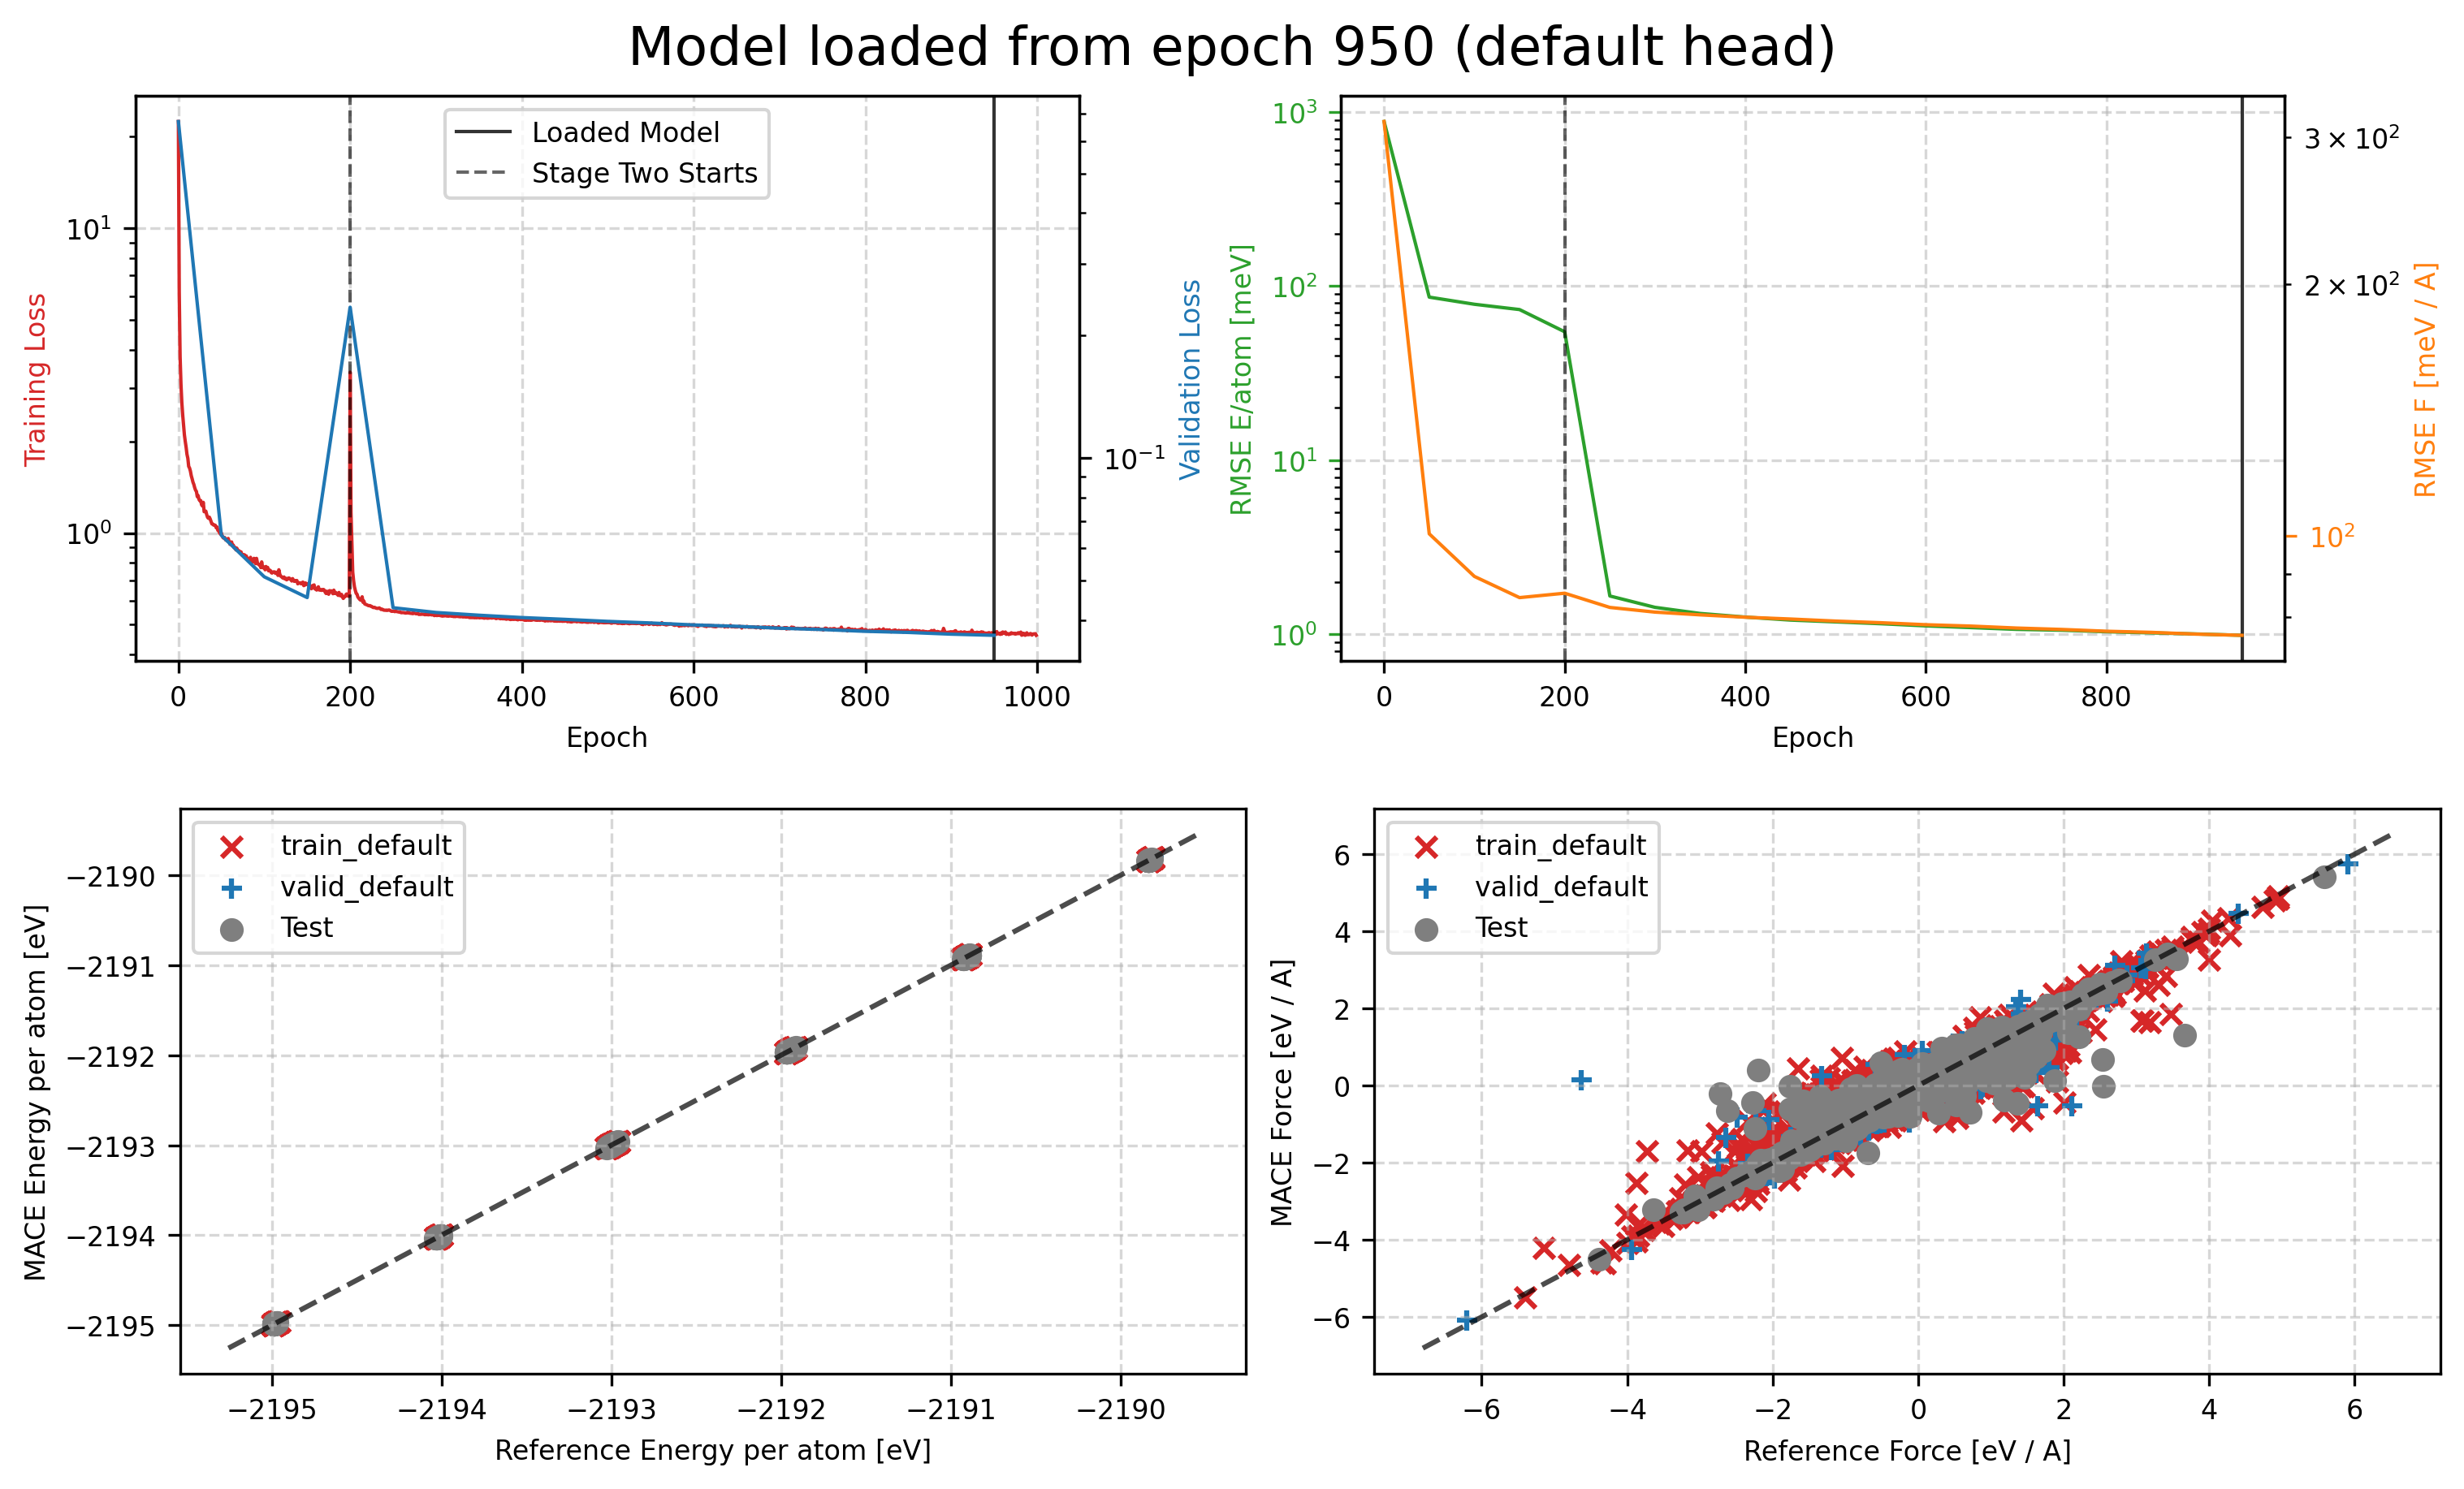
\includegraphics[width=\linewidth,height=0.42\textheight,keepaspectratio]{figure_pages/assets/fig_180.png}
\caption{Legacy supplementary-information figure. This page shows the candidate output ``1 scratch mace l1 0802 run 123 train default stage two'' within the audited LEGACY-SI family. The panel identity, source scope, and current status are retained in the accompanying evidence matrix.}
\label{fig:candidate_180}
\end{figure}
\textbf{Results text draft.} The figure is retained for SI provenance and reconciliation with the revised source ledger. The displayed result is not assumed to inherit the current audit status automatically.
\textbf{Discussion and boundary.} Use only with an explicit historical or audited label and a checked underlying source chain.
\textbf{Article placement.} Proposed article location: Legacy SI.
\textbf{Reviewer linkage:} overall status NO\_DIRECT\_REVIEWER\_FIGURE\_LINK.
No direct reviewer-response figure linkage was identified; this page is retained for scientific/article audit rather than as a direct reviewer response.
\textbf{Evidence pointers.}
No data/script/text candidate was recorded in the matrix; resolve this gap before manuscript promotion.
\statusline{\textbf{Audit gap / next action:} Image-only or historical source chain not closed}
\vfill
\clearpage
\section{FIG-181 --- 2 finetuned mace multihead0804 run 123 train default stage two}
\label{figpage:fig-181}
\textbf{Group:} LEGACY-SI\quad \textbf{Evidence chain:} partial\quad \textbf{Status:} publication
\begin{figure}[H]
\centering
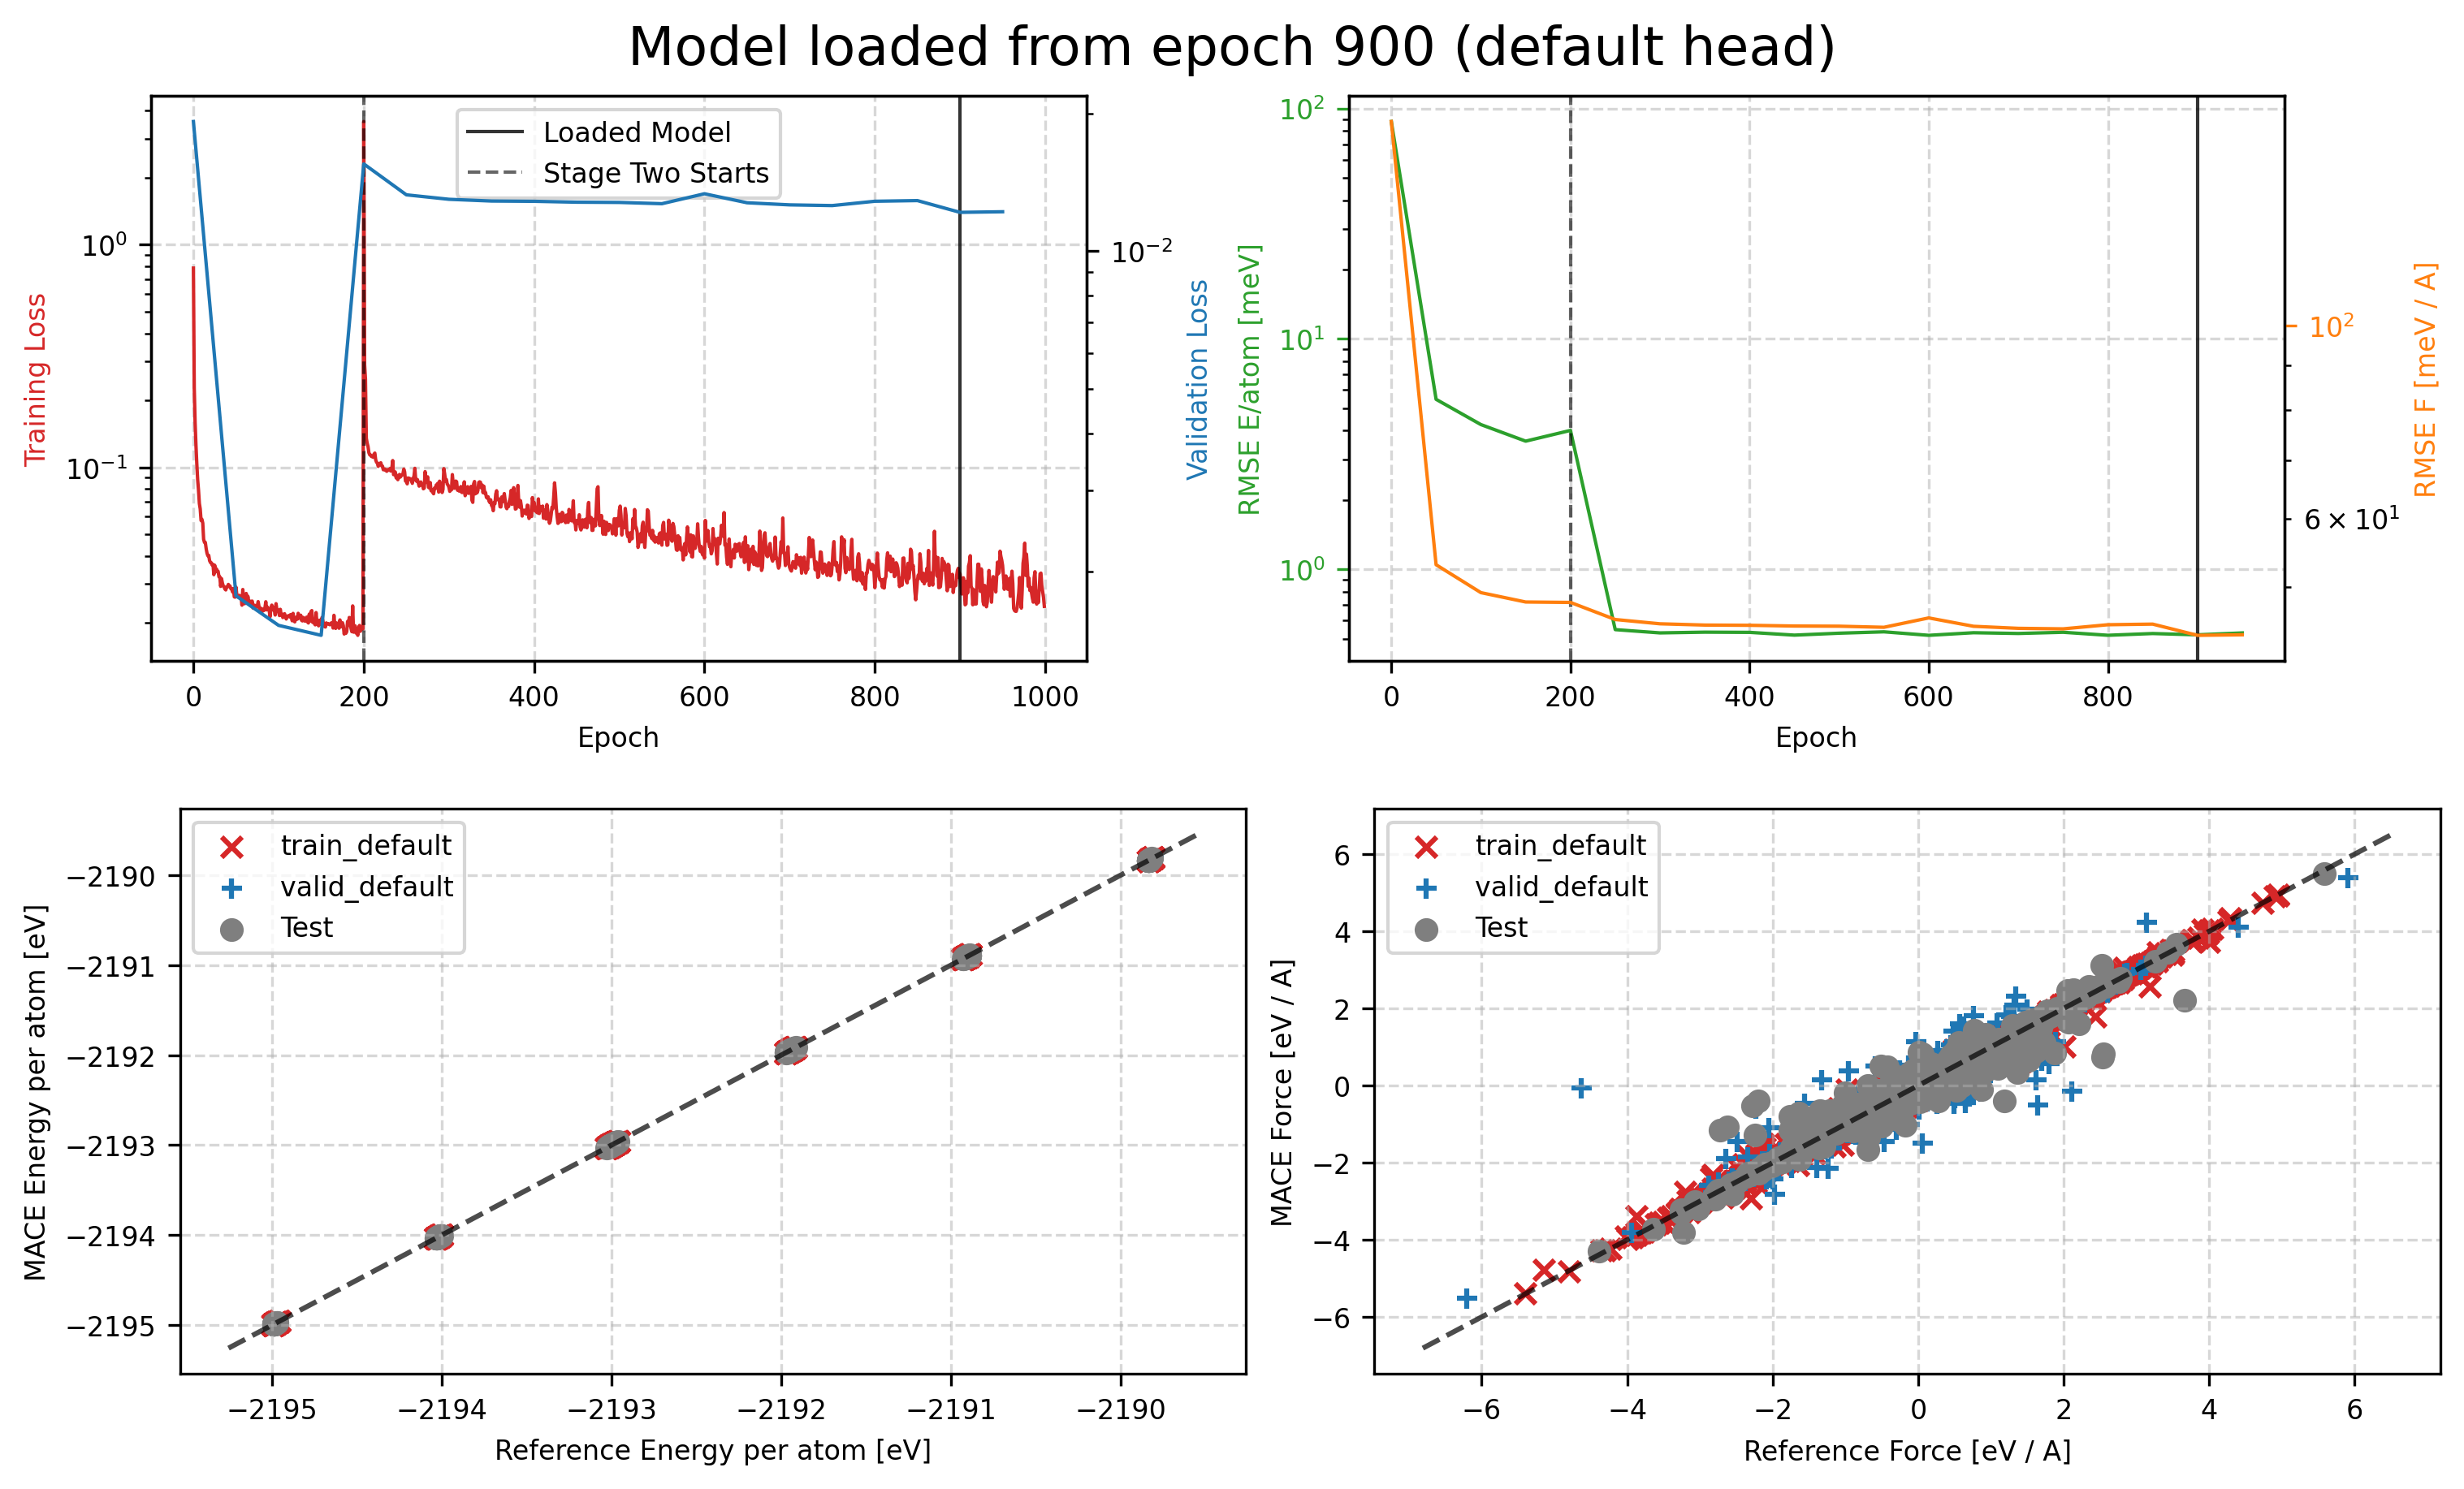
\includegraphics[width=\linewidth,height=0.42\textheight,keepaspectratio]{figure_pages/assets/fig_181.png}
\caption{Legacy supplementary-information figure. This page shows the candidate output ``2 finetuned mace multihead0804 run 123 train default stage two'' within the audited LEGACY-SI family. The panel identity, source scope, and current status are retained in the accompanying evidence matrix.}
\label{fig:candidate_181}
\end{figure}
\textbf{Results text draft.} The figure is retained for SI provenance and reconciliation with the revised source ledger. The displayed result is not assumed to inherit the current audit status automatically.
\textbf{Discussion and boundary.} Use only with an explicit historical or audited label and a checked underlying source chain.
\textbf{Article placement.} Proposed article location: Legacy SI.
\textbf{Reviewer linkage:} overall status NO\_DIRECT\_REVIEWER\_FIGURE\_LINK.
No direct reviewer-response figure linkage was identified; this page is retained for scientific/article audit rather than as a direct reviewer response.
\textbf{Evidence pointers.}
No data/script/text candidate was recorded in the matrix; resolve this gap before manuscript promotion.
\statusline{\textbf{Audit gap / next action:} Image-only or historical source chain not closed}
\vfill
\clearpage
\section{FIG-182 --- 3 finetuned mace multihead0804 run 123 train default stage two multi t}
\label{figpage:fig-182}
\textbf{Group:} LEGACY-SI\quad \textbf{Evidence chain:} partial\quad \textbf{Status:} publication
\begin{figure}[H]
\centering
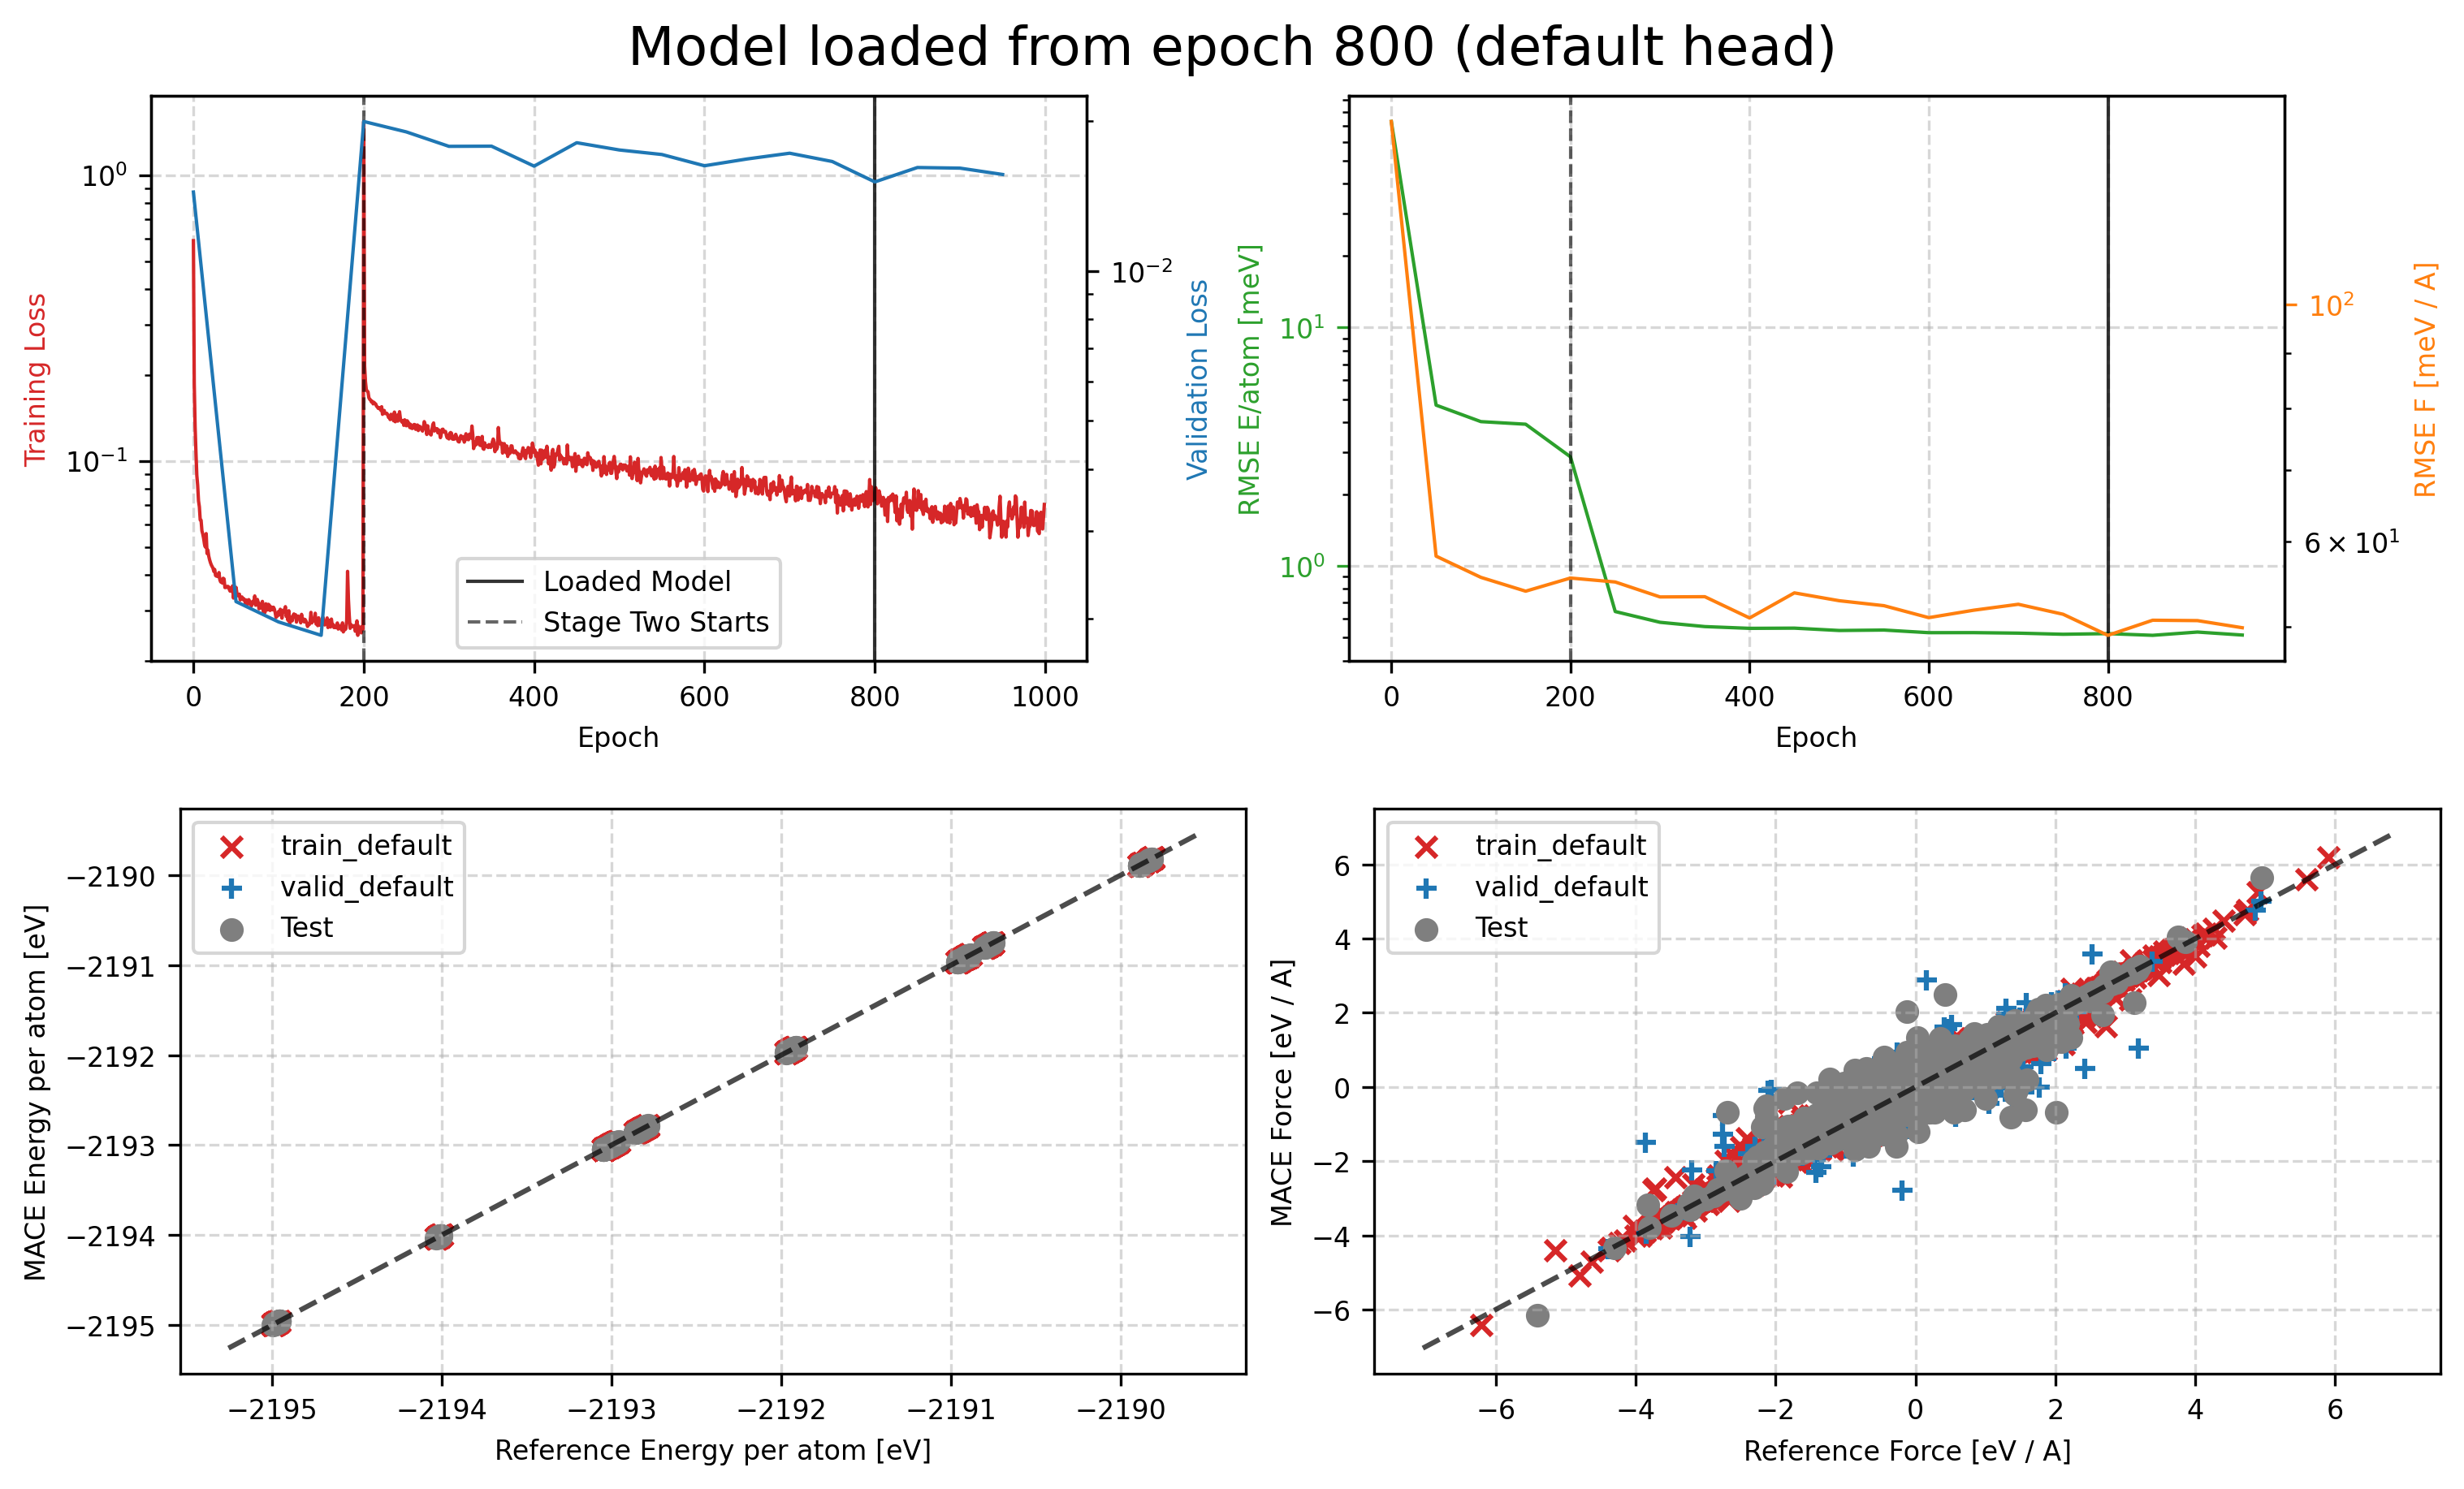
\includegraphics[width=\linewidth,height=0.42\textheight,keepaspectratio]{figure_pages/assets/fig_182.png}
\caption{Legacy supplementary-information figure. This page shows the candidate output ``3 finetuned mace multihead0804 run 123 train default stage two multi t'' within the audited LEGACY-SI family. The panel identity, source scope, and current status are retained in the accompanying evidence matrix.}
\label{fig:candidate_182}
\end{figure}
\textbf{Results text draft.} The figure is retained for SI provenance and reconciliation with the revised source ledger. The displayed result is not assumed to inherit the current audit status automatically.
\textbf{Discussion and boundary.} Use only with an explicit historical or audited label and a checked underlying source chain.
\textbf{Article placement.} Proposed article location: Legacy SI.
\textbf{Reviewer linkage:} overall status NO\_DIRECT\_REVIEWER\_FIGURE\_LINK.
No direct reviewer-response figure linkage was identified; this page is retained for scientific/article audit rather than as a direct reviewer response.
\textbf{Evidence pointers.}
No data/script/text candidate was recorded in the matrix; resolve this gap before manuscript promotion.
\statusline{\textbf{Audit gap / next action:} Image-only or historical source chain not closed}
\vfill
\clearpage
\section{FIG-183 --- Neurips2025 ai4mat figure3 2}
\label{figpage:fig-183}
\textbf{Group:} LEGACY-SI\quad \textbf{Evidence chain:} partial\quad \textbf{Status:} publication
\begin{figure}[H]
\centering
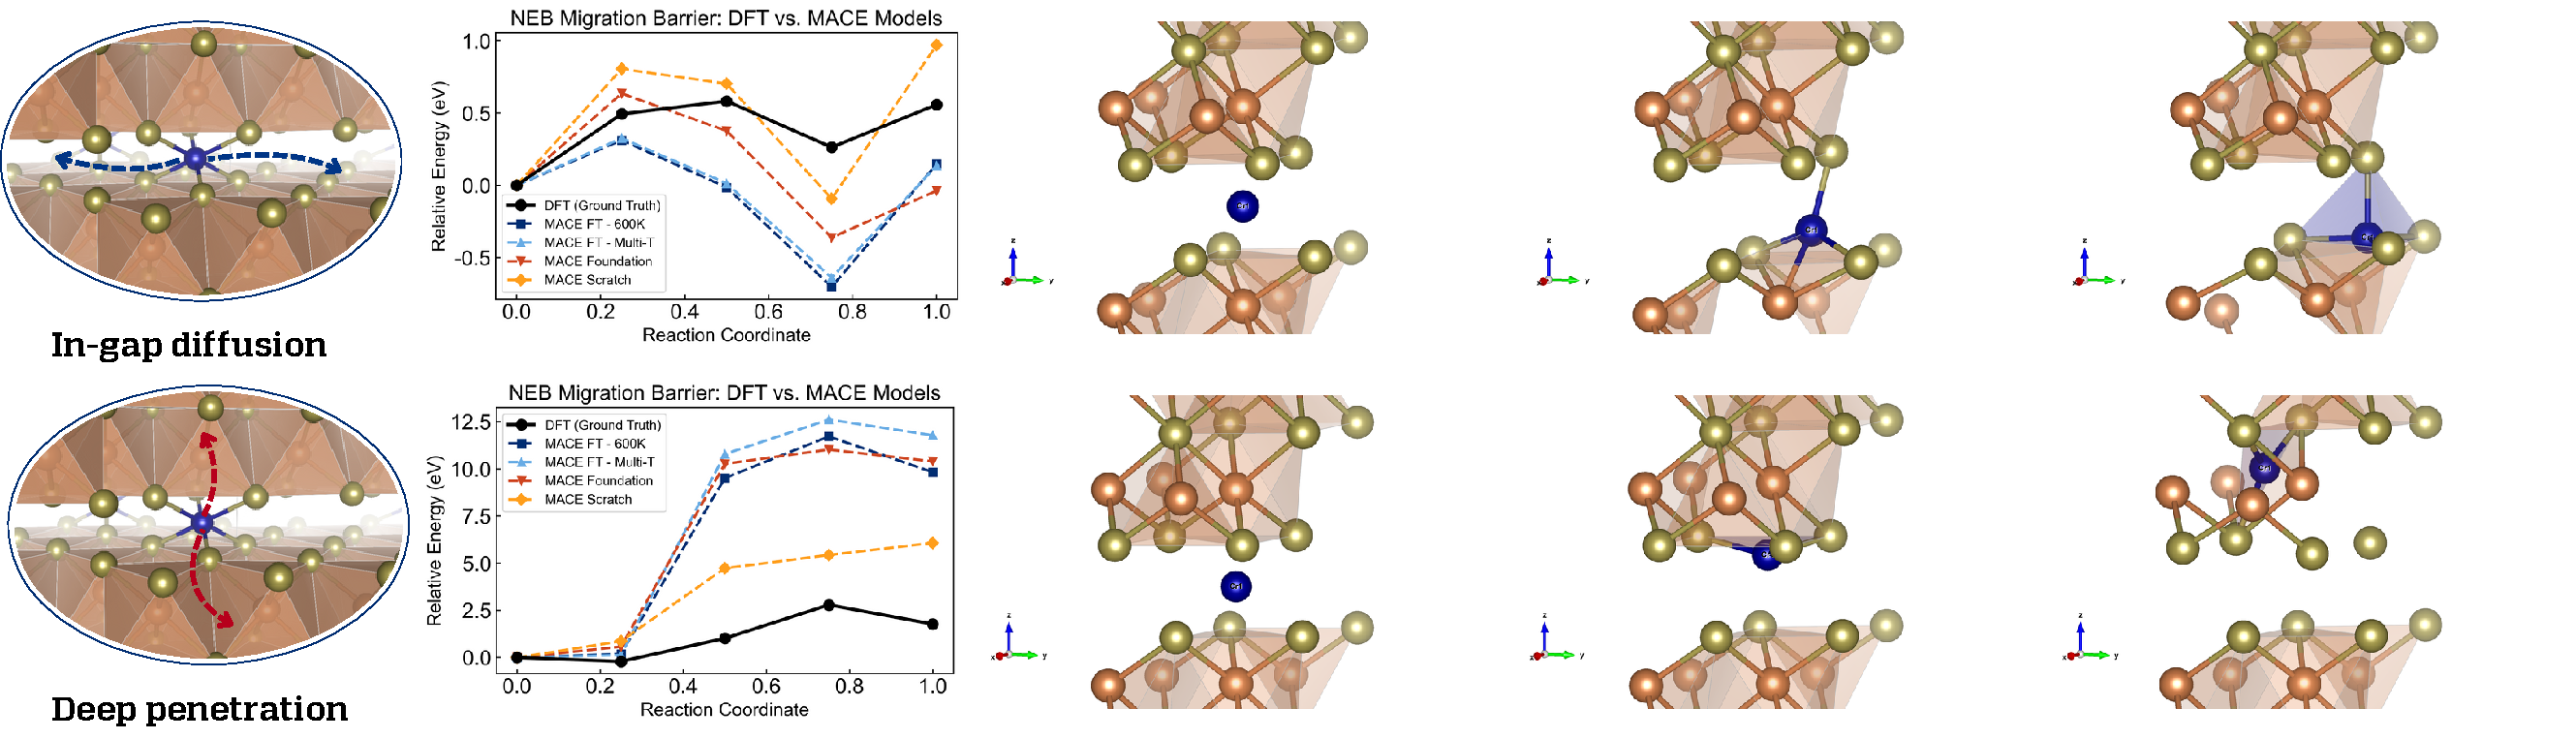
\includegraphics[width=\linewidth,height=0.42\textheight,keepaspectratio]{figure_pages/assets/fig_183.pdf}
\caption{Legacy supplementary-information figure. This page shows the candidate output ``Neurips2025 ai4mat figure3 2'' within the audited LEGACY-SI family. The panel identity, source scope, and current status are retained in the accompanying evidence matrix.}
\label{fig:candidate_183}
\end{figure}
\textbf{Results text draft.} The figure is retained for SI provenance and reconciliation with the revised source ledger. The displayed result is not assumed to inherit the current audit status automatically.
\textbf{Discussion and boundary.} Use only with an explicit historical or audited label and a checked underlying source chain.
\textbf{Article placement.} Proposed article location: Legacy SI.
\textbf{Reviewer linkage:} overall status NO\_DIRECT\_REVIEWER\_FIGURE\_LINK.
No direct reviewer-response figure linkage was identified; this page is retained for scientific/article audit rather than as a direct reviewer response.
\textbf{Evidence pointers.}
No data/script/text candidate was recorded in the matrix; resolve this gap before manuscript promotion.
\statusline{\textbf{Audit gap / next action:} Image-only or historical source chain not closed}
\vfill
\clearpage
\section{FIG-184 --- Response to reviewers}
\label{figpage:fig-184}
\textbf{Group:} COMPILED-DOCUMENT\quad \textbf{Evidence chain:} compiled document\quad \textbf{Status:} publication
\begin{figure}[H]
\centering
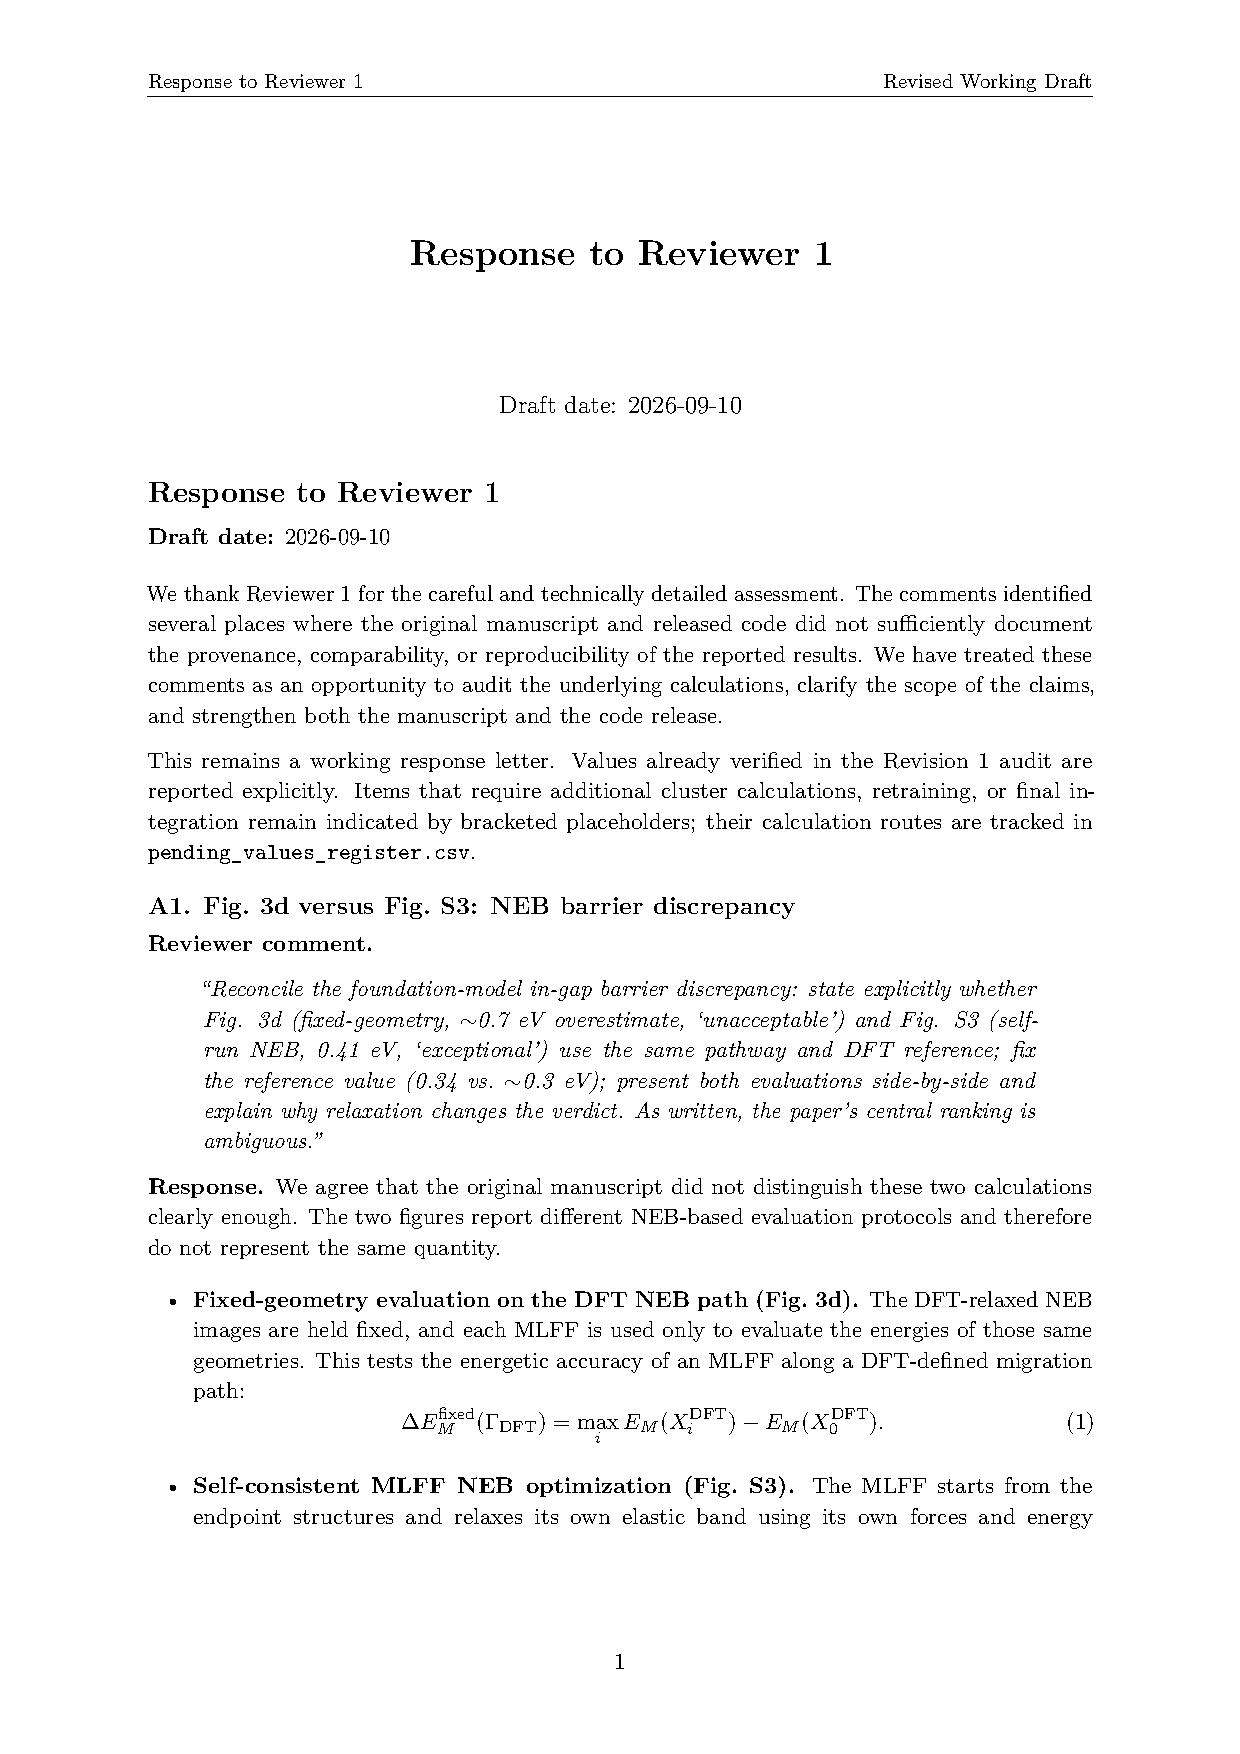
\includegraphics[width=\linewidth,height=0.42\textheight,keepaspectratio]{figure_pages/assets/fig_184.pdf}
\caption{Compiled manuscript or response artifact retained as document-level evidence. This page shows the candidate output ``Response to reviewers'' within the audited COMPILED-DOCUMENT family. The panel identity, source scope, and current status are retained in the accompanying evidence matrix.}
\label{fig:candidate_184}
\end{figure}
\textbf{Results text draft.} This entry is a compiled document rather than an independent scientific figure. It is retained because it may contain figure captions, rendered panels, or response language that must be reconciled with the source ledger.
\textbf{Discussion and boundary.} Use only as document provenance; cite the underlying figure and reproducible source chain for scientific claims.
\textbf{Article placement.} Proposed article location: Response or manuscript.
\textbf{Reviewer linkage:} overall status NO\_DIRECT\_REVIEWER\_FIGURE\_LINK.
No direct reviewer-response figure linkage was identified; this page is retained for scientific/article audit rather than as a direct reviewer response.
\textbf{Evidence pointers.}
\begin{itemize}[leftmargin=1.4em,noitemsep]
\item Caption/text source: \begingroup\scriptsize\url{paper/README.md}\endgroup
\item Caption/text source: \begingroup\scriptsize\url{paper/paper/response_to_reviewers.log}\endgroup
\end{itemize}
\statusline{\textbf{Audit gap / next action:} Not an independent figure}
\vfill
\clearpage
\section{FIG-185 --- Response to reviewers}
\label{figpage:fig-185}
\textbf{Group:} COMPILED-DOCUMENT\quad \textbf{Evidence chain:} compiled document\quad \textbf{Status:} publication
\begin{figure}[H]
\centering
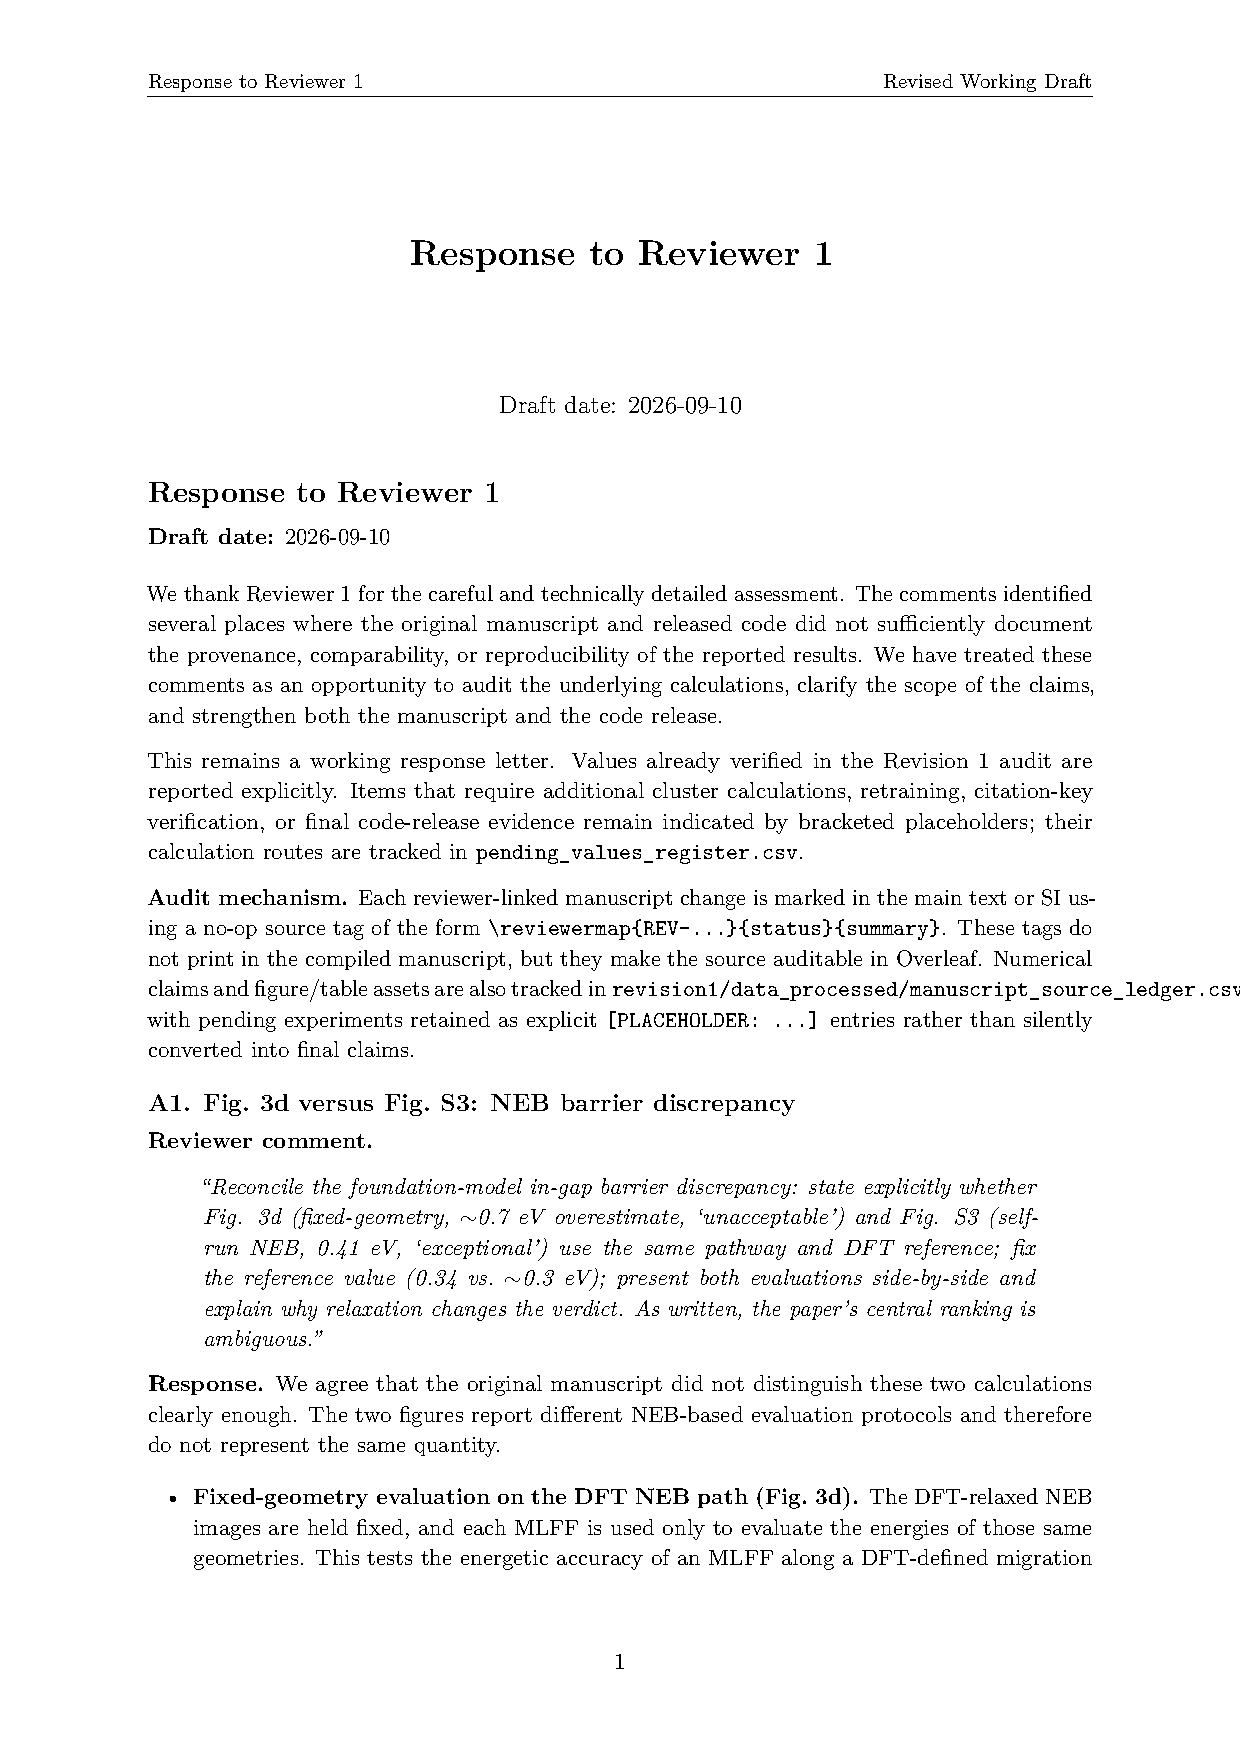
\includegraphics[width=\linewidth,height=0.42\textheight,keepaspectratio]{figure_pages/assets/fig_185.pdf}
\caption{Compiled manuscript or response artifact retained as document-level evidence. This page shows the candidate output ``Response to reviewers'' within the audited COMPILED-DOCUMENT family. The panel identity, source scope, and current status are retained in the accompanying evidence matrix.}
\label{fig:candidate_185}
\end{figure}
\textbf{Results text draft.} This entry is a compiled document rather than an independent scientific figure. It is retained because it may contain figure captions, rendered panels, or response language that must be reconciled with the source ledger.
\textbf{Discussion and boundary.} Use only as document provenance; cite the underlying figure and reproducible source chain for scientific claims.
\textbf{Article placement.} Proposed article location: Response or manuscript.
\textbf{Reviewer linkage:} overall status NO\_DIRECT\_REVIEWER\_FIGURE\_LINK.
No direct reviewer-response figure linkage was identified; this page is retained for scientific/article audit rather than as a direct reviewer response.
\textbf{Evidence pointers.}
\begin{itemize}[leftmargin=1.4em,noitemsep]
\item Data/processed: \begingroup\scriptsize\url{paper/paper/response_to_reviewers/revision_pack_2026-09-10/pending_values_register.csv}\endgroup
\item Plot/processing script: \begingroup\scriptsize\url{paper/paper/response_to_reviewers/revision_pack_2026-09-10/apply_reviewer_markers.py}\endgroup
\item Caption/text source: \begingroup\scriptsize\url{paper/paper/response_to_reviewers/overleaf_applied_changes_2026-09-11.md}\endgroup
\item Caption/text source: \begingroup\scriptsize\url{paper/paper/response_to_reviewers/proposed_text_edits.md}\endgroup
\end{itemize}
\statusline{\textbf{Audit gap / next action:} Not an independent figure}
\vfill
\clearpage
\section{FIG-186 --- Fig1 campaign overview}
\label{figpage:fig-186}
\textbf{Group:} REV1-APPENDIX\quad \textbf{Evidence chain:} traceable\quad \textbf{Status:} publication
\begin{figure}[H]
\centering
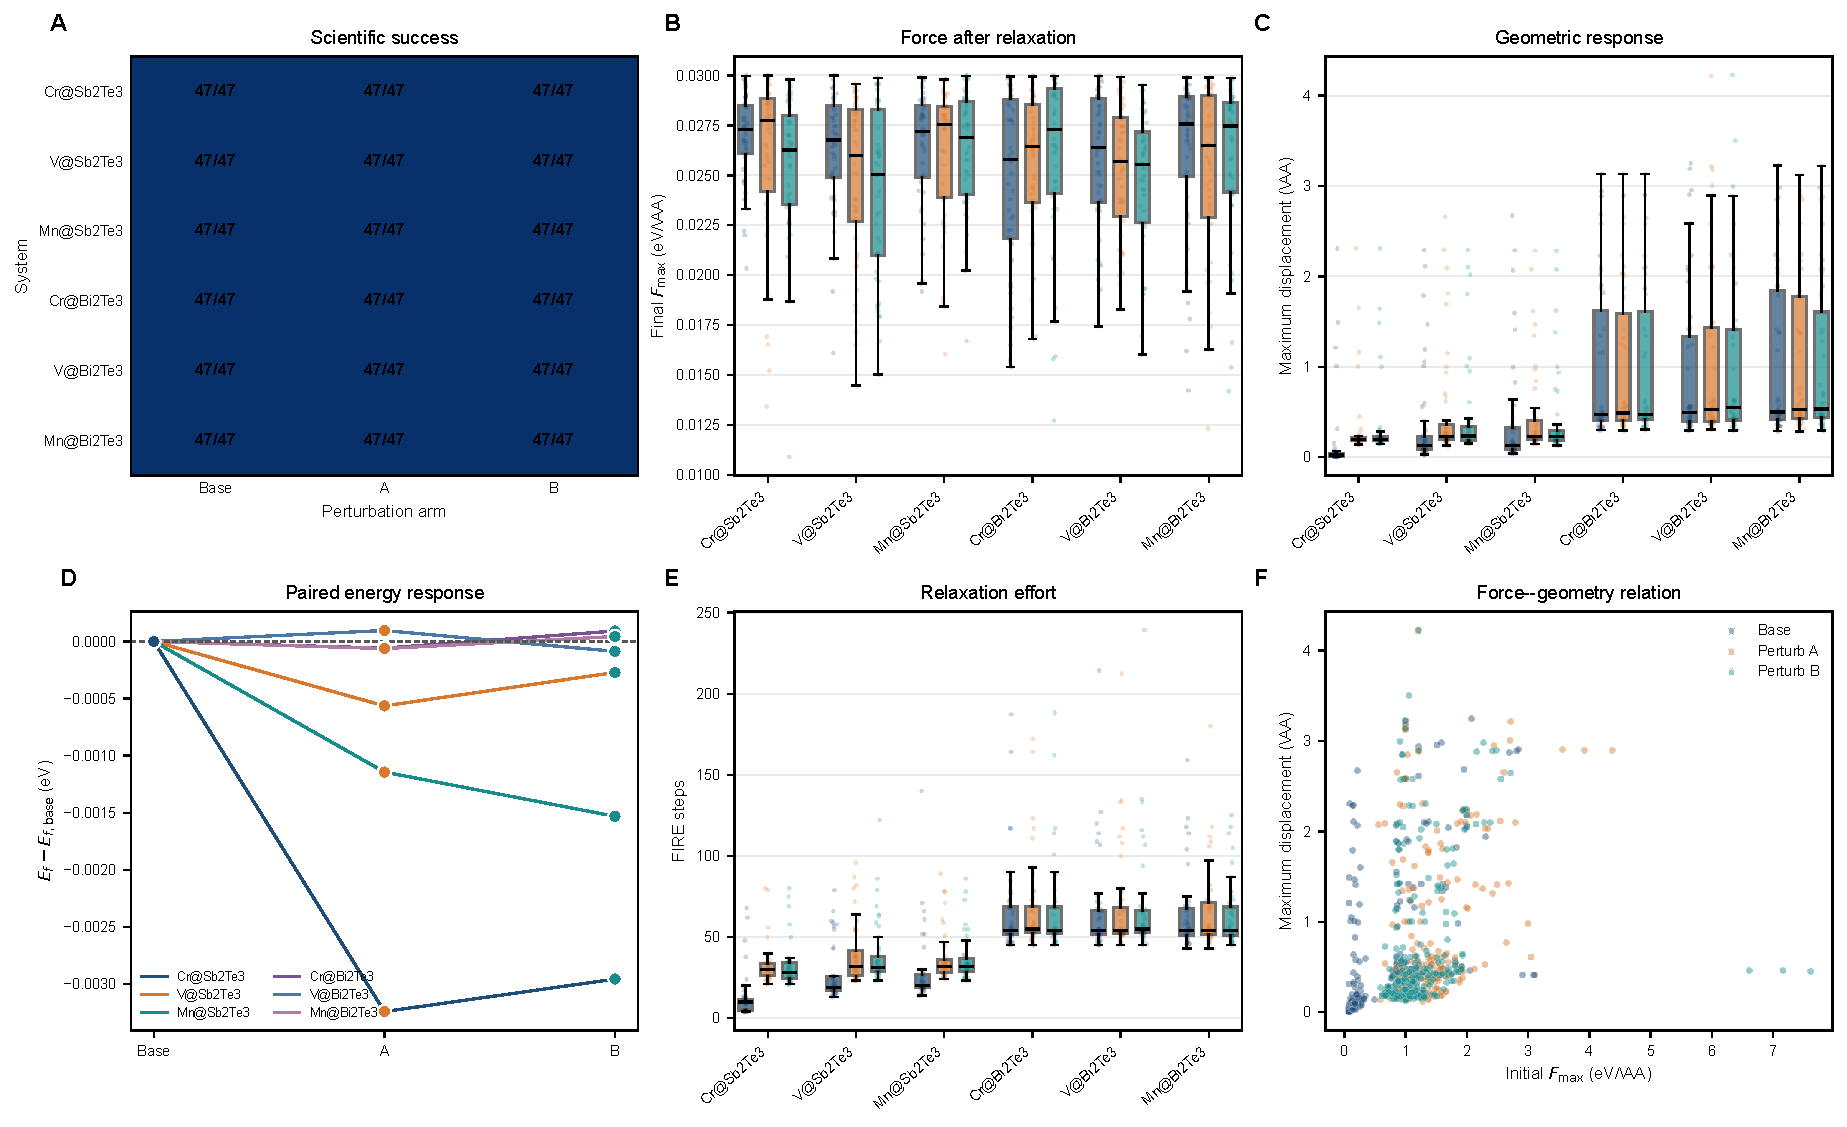
\includegraphics[width=\linewidth,height=0.42\textheight,keepaspectratio]{figure_pages/assets/fig_186.pdf}
\caption{Revision\textasciitilde{}1 appendix figure. This page shows the candidate output ``Fig1 campaign overview'' within the audited REV1-APPENDIX family. The panel identity, source scope, and current status are retained in the accompanying evidence matrix.}
\label{fig:candidate_186}
\end{figure}
\textbf{Results text draft.} The figure is part of the Revision\textasciitilde{}1 appendix evidence set and is presented with the current source-ledger status.
\textbf{Discussion and boundary.} The appendix placement is appropriate while the corresponding claim, data scope, and uncertainty treatment are being finalized.
\textbf{Article placement.} Proposed article location: SI endpoint-relaxation appendix.
\textbf{Reviewer linkage:} overall status NO\_DIRECT\_REVIEWER\_FIGURE\_LINK.
No direct reviewer-response figure linkage was identified; this page is retained for scientific/article audit rather than as a direct reviewer response.
\textbf{Evidence pointers.}
\begin{itemize}[leftmargin=1.4em,noitemsep]
\item Caption/text source: \begingroup\scriptsize\url{paper/paper/revision1/appendix/README.md}\endgroup
\item Caption/text source: \begingroup\scriptsize\url{paper/paper/revision1/appendix/endpoint_perturbation_appendix.tex}\endgroup
\end{itemize}
\statusline{\textbf{Audit gap / next action:} Caption is in endpoint\_perturbation\_appendix.tex; confirm final compiled placement}
\vfill
\clearpage
\section{FIG-187 --- Fig2 perturbation response}
\label{figpage:fig-187}
\textbf{Group:} REV1-APPENDIX\quad \textbf{Evidence chain:} traceable\quad \textbf{Status:} publication
\begin{figure}[H]
\centering
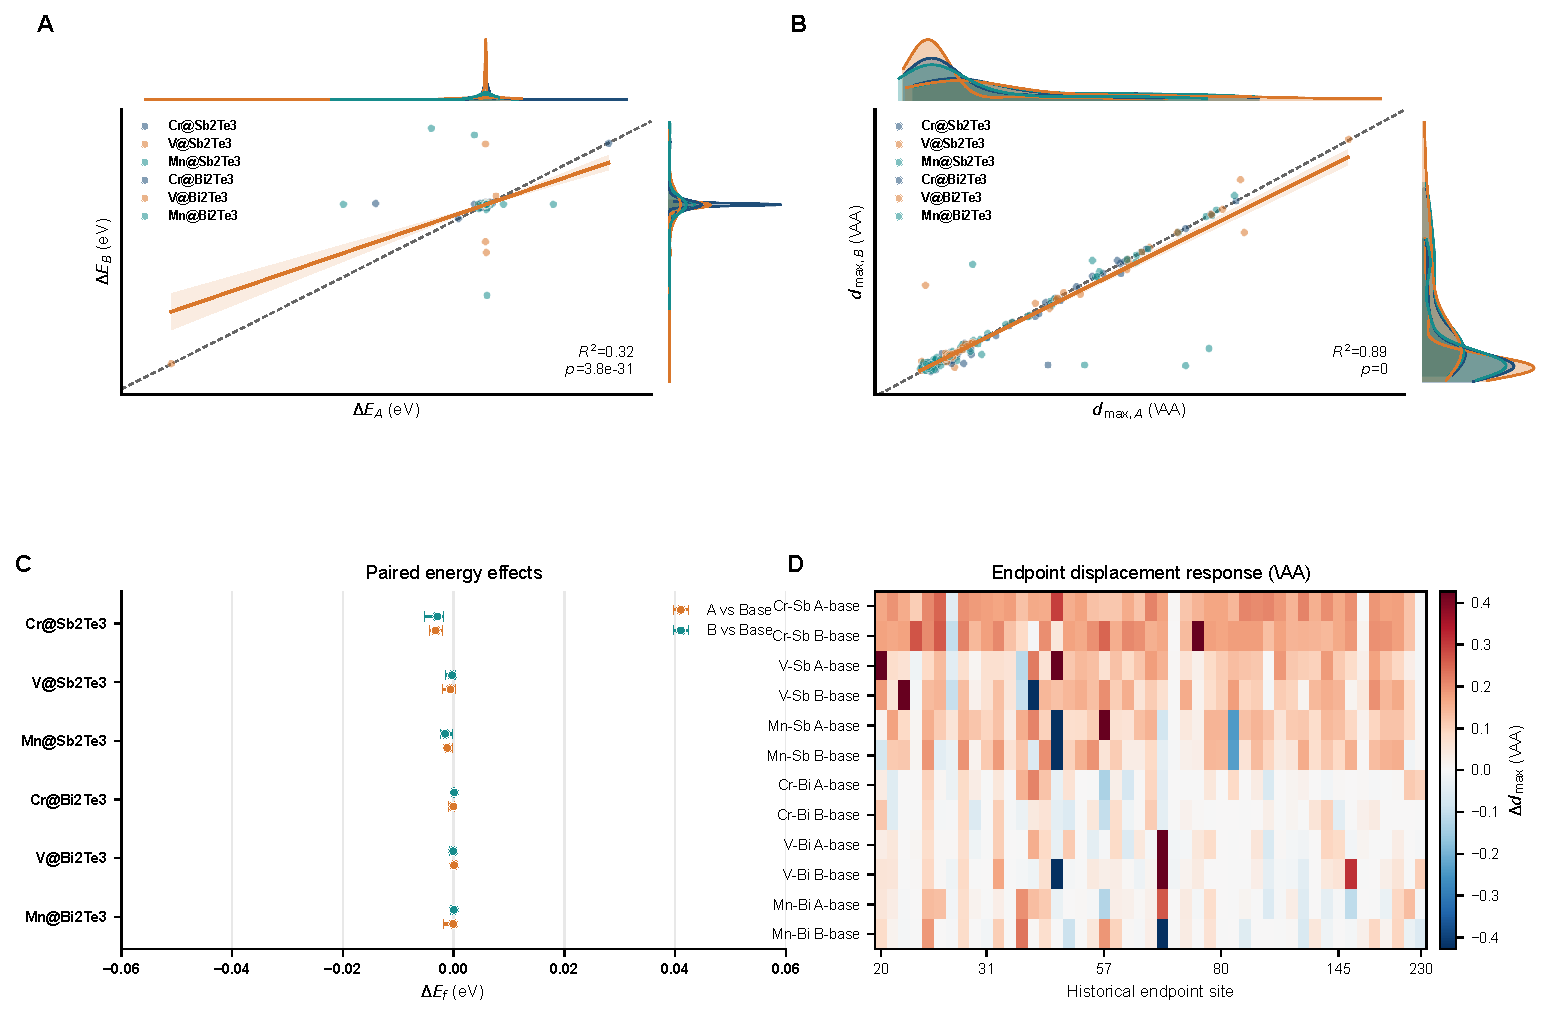
\includegraphics[width=\linewidth,height=0.42\textheight,keepaspectratio]{figure_pages/assets/fig_187.pdf}
\caption{Revision\textasciitilde{}1 appendix figure. This page shows the candidate output ``Fig2 perturbation response'' within the audited REV1-APPENDIX family. The panel identity, source scope, and current status are retained in the accompanying evidence matrix.}
\label{fig:candidate_187}
\end{figure}
\textbf{Results text draft.} The figure is part of the Revision\textasciitilde{}1 appendix evidence set and is presented with the current source-ledger status.
\textbf{Discussion and boundary.} The appendix placement is appropriate while the corresponding claim, data scope, and uncertainty treatment are being finalized.
\textbf{Article placement.} Proposed article location: SI endpoint-relaxation appendix.
\textbf{Reviewer linkage:} overall status NO\_DIRECT\_REVIEWER\_FIGURE\_LINK.
No direct reviewer-response figure linkage was identified; this page is retained for scientific/article audit rather than as a direct reviewer response.
\textbf{Evidence pointers.}
\begin{itemize}[leftmargin=1.4em,noitemsep]
\item Caption/text source: \begingroup\scriptsize\url{paper/paper/revision1/appendix/README.md}\endgroup
\item Caption/text source: \begingroup\scriptsize\url{paper/paper/revision1/appendix/endpoint_perturbation_appendix.tex}\endgroup
\end{itemize}
\statusline{\textbf{Audit gap / next action:} Caption is in endpoint\_perturbation\_appendix.tex; confirm final compiled placement}
\vfill
\clearpage
\section{FIG-188 --- Fig3 interaction and site maps}
\label{figpage:fig-188}
\textbf{Group:} REV1-APPENDIX\quad \textbf{Evidence chain:} traceable\quad \textbf{Status:} publication
\begin{figure}[H]
\centering
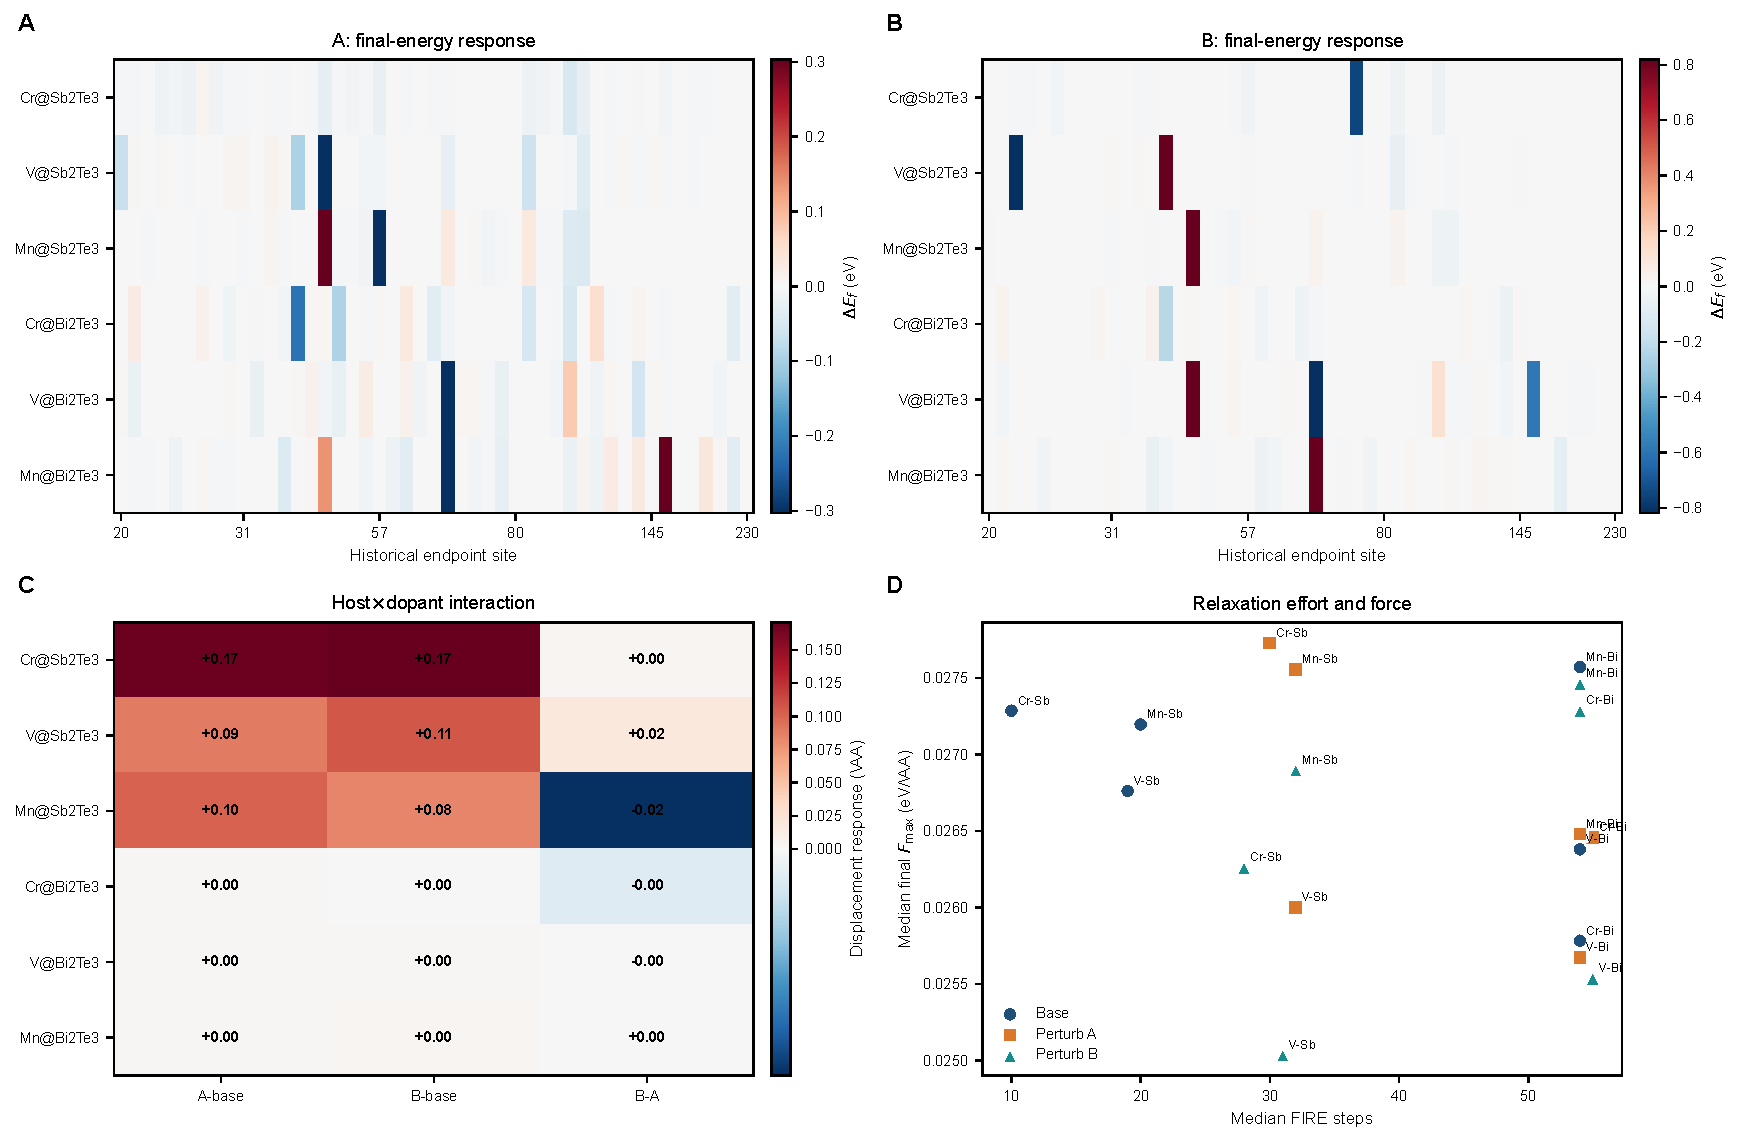
\includegraphics[width=\linewidth,height=0.42\textheight,keepaspectratio]{figure_pages/assets/fig_188.pdf}
\caption{Revision\textasciitilde{}1 appendix figure. This page shows the candidate output ``Fig3 interaction and site maps'' within the audited REV1-APPENDIX family. The panel identity, source scope, and current status are retained in the accompanying evidence matrix.}
\label{fig:candidate_188}
\end{figure}
\textbf{Results text draft.} The figure is part of the Revision\textasciitilde{}1 appendix evidence set and is presented with the current source-ledger status.
\textbf{Discussion and boundary.} The appendix placement is appropriate while the corresponding claim, data scope, and uncertainty treatment are being finalized.
\textbf{Article placement.} Proposed article location: SI endpoint-relaxation appendix.
\textbf{Reviewer linkage:} overall status NO\_DIRECT\_REVIEWER\_FIGURE\_LINK.
No direct reviewer-response figure linkage was identified; this page is retained for scientific/article audit rather than as a direct reviewer response.
\textbf{Evidence pointers.}
\begin{itemize}[leftmargin=1.4em,noitemsep]
\item Caption/text source: \begingroup\scriptsize\url{paper/paper/revision1/appendix/README.md}\endgroup
\item Caption/text source: \begingroup\scriptsize\url{paper/paper/revision1/appendix/endpoint_perturbation_appendix.tex}\endgroup
\end{itemize}
\statusline{\textbf{Audit gap / next action:} Caption is in endpoint\_perturbation\_appendix.tex; confirm final compiled placement}
\vfill
\clearpage
\section{FIG-189 --- Fig6 shap revised}
\label{figpage:fig-189}
\textbf{Group:} REV1-ARTICLE\quad \textbf{Evidence chain:} traceable\quad \textbf{Status:} publication
\begin{figure}[H]
\centering
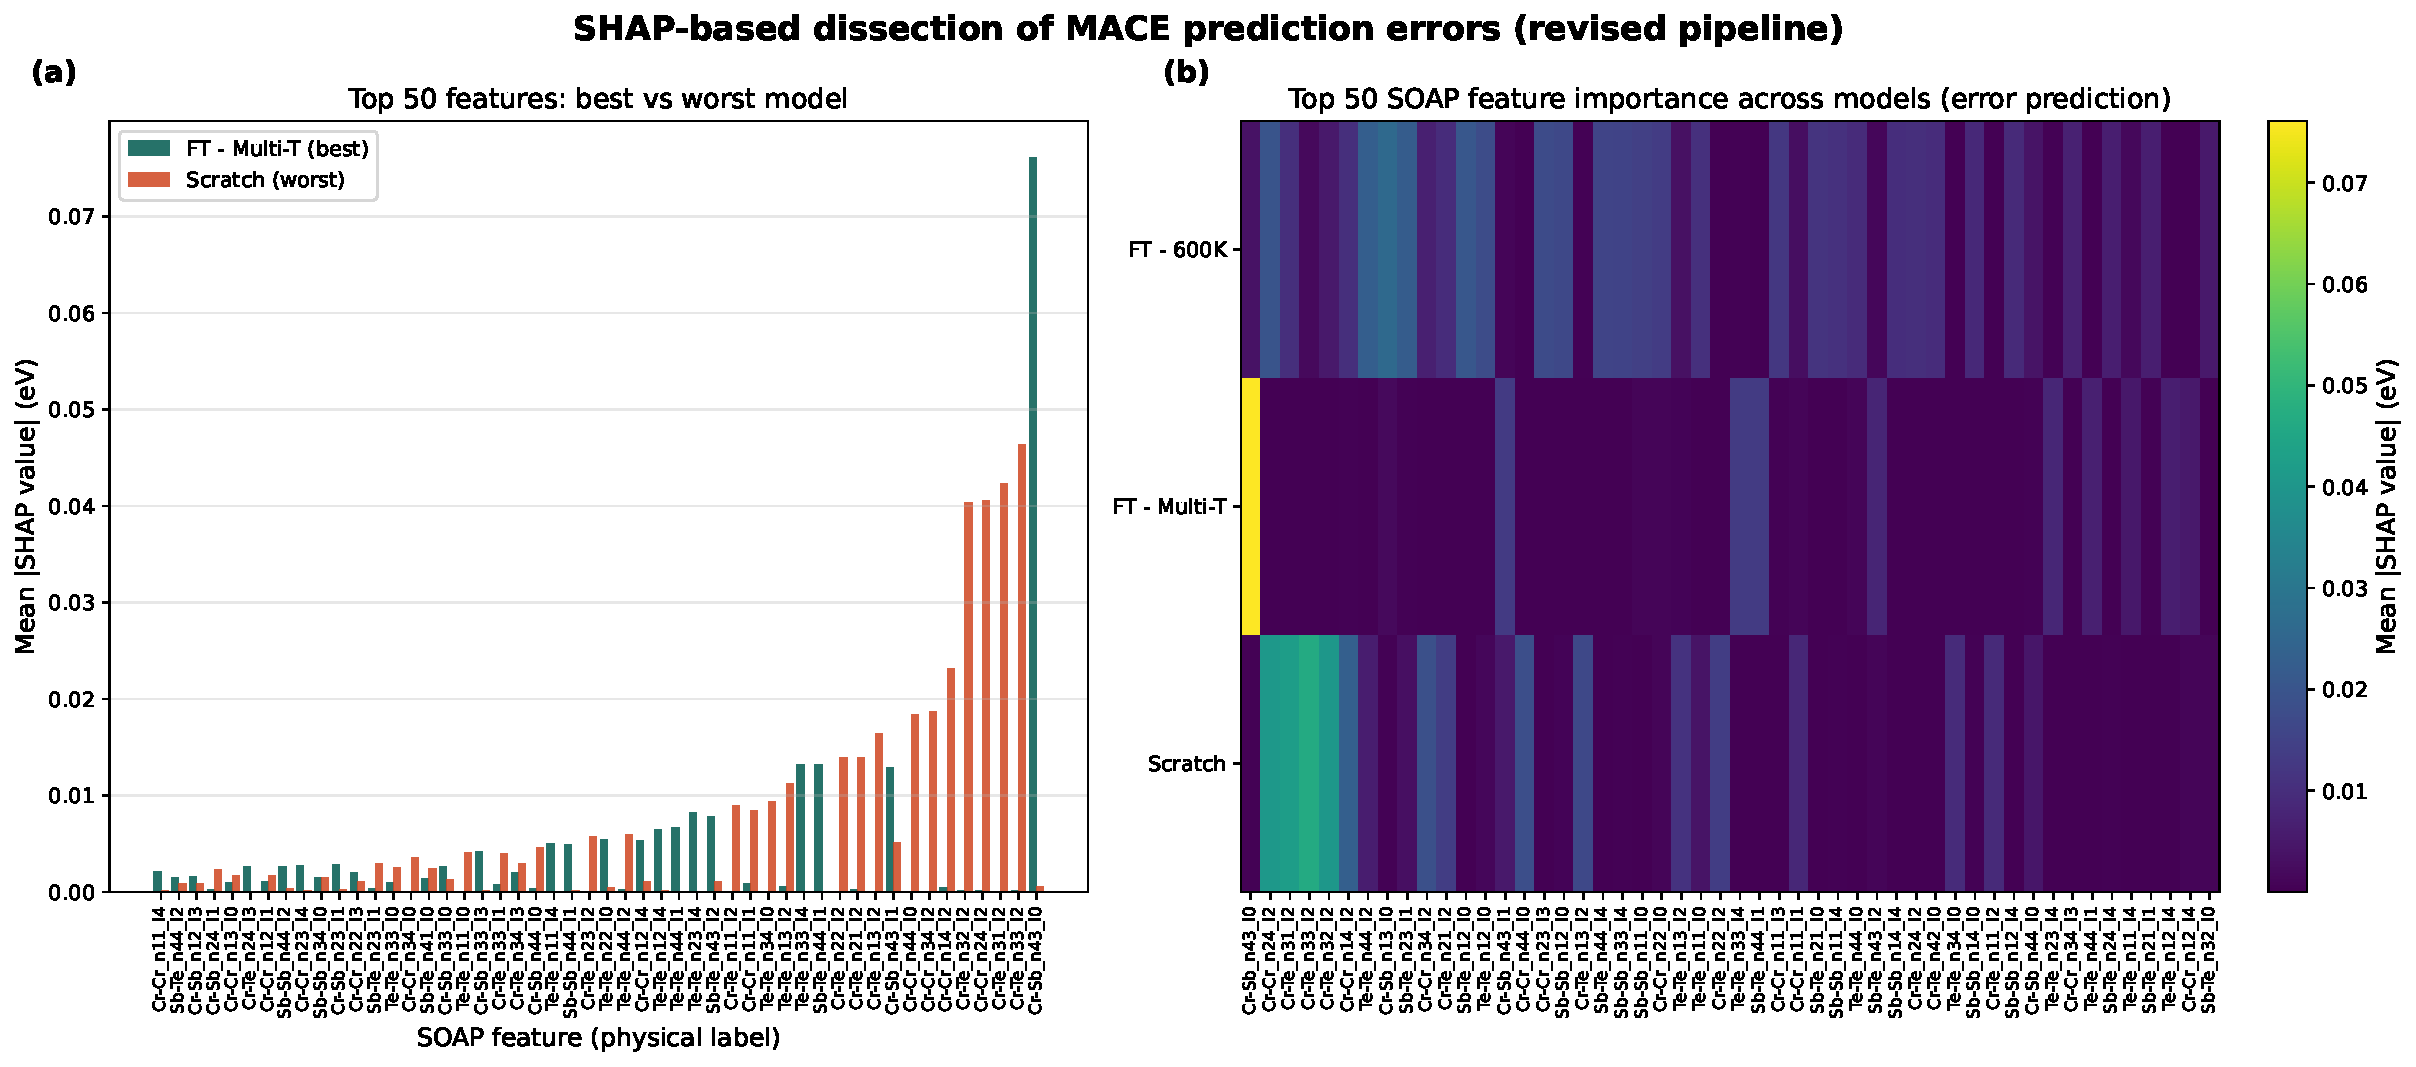
\includegraphics[width=\linewidth,height=0.42\textheight,keepaspectratio]{figure_pages/assets/fig_189.pdf}
\caption{Revision\textasciitilde{}1 article figure. This page shows the candidate output ``Fig6 shap revised'' within the audited REV1-ARTICLE family. The panel identity, source scope, and current status are retained in the accompanying evidence matrix.}
\label{fig:candidate_189}
\end{figure}
\textbf{Results text draft.} The figure is already associated with the Revision\textasciitilde{}1 article structure and is presented here for page-level caption and prose review.
\textbf{Discussion and boundary.} Before final submission, confirm that the caption, Results text, and source ledger agree on the current audited values and exclusions.
\textbf{Article placement.} Proposed article location: Mapped by sn-article-final.tex or sn-article-SI.tex.
\textbf{Reviewer linkage:} overall status PARTIAL.
\begin{itemize}[leftmargin=1.4em,noitemsep]
\item \textbf{REV-A6 (PARTIAL):} Soften t-SNE/PHATE and SHAP interpretation claims and add projection/original-space and surrogate-fidelity checks. \emph{Completed:} Projection sensitivity, original-descriptor-space separation, and per-model cross-validated surrogate R2 are available; the text is scoped to descriptive/surrogate evidence. \emph{Still required:} A direct MACE Cr-Cr perturbation test remains pending if a causal claim about the dominant feature is desired; otherwise retain the surrogate-scoped wording.
\item \textbf{REV-C13 (PARTIAL):} Make the SHAP pipeline and advertised repository artifacts reproducible rather than leaving empty stubs. \emph{Completed:} The corrected SHAP inputs, scripts, lineage, and locked revised outputs are present for the declared three-model/150-frame scope. \emph{Still required:} Close the final release/empty-stub audit and reconcile the independent rerun with the locked historical CSV before claiming exact end-to-end regeneration.
\end{itemize}
\textbf{Evidence pointers.}
\begin{itemize}[leftmargin=1.4em,noitemsep]
\item Caption/text source: \begingroup\scriptsize\url{paper/paper/revision1/benchmark_formalization.tex}\endgroup
\item Caption/text source: \begingroup\scriptsize\url{paper/paper/revision1/response_to_reviewers.log}\endgroup
\end{itemize}
\statusline{\textbf{Audit gap / next action:} Check figure source ledger and exact generator; some assets are compiled from older workflows}
\vfill
\clearpage
\section{FIG-190 --- Figs dft neb mep profiles}
\label{figpage:fig-190}
\textbf{Group:} REV1-ARTICLE\quad \textbf{Evidence chain:} traceable\quad \textbf{Status:} publication;comparison
\begin{figure}[H]
\centering
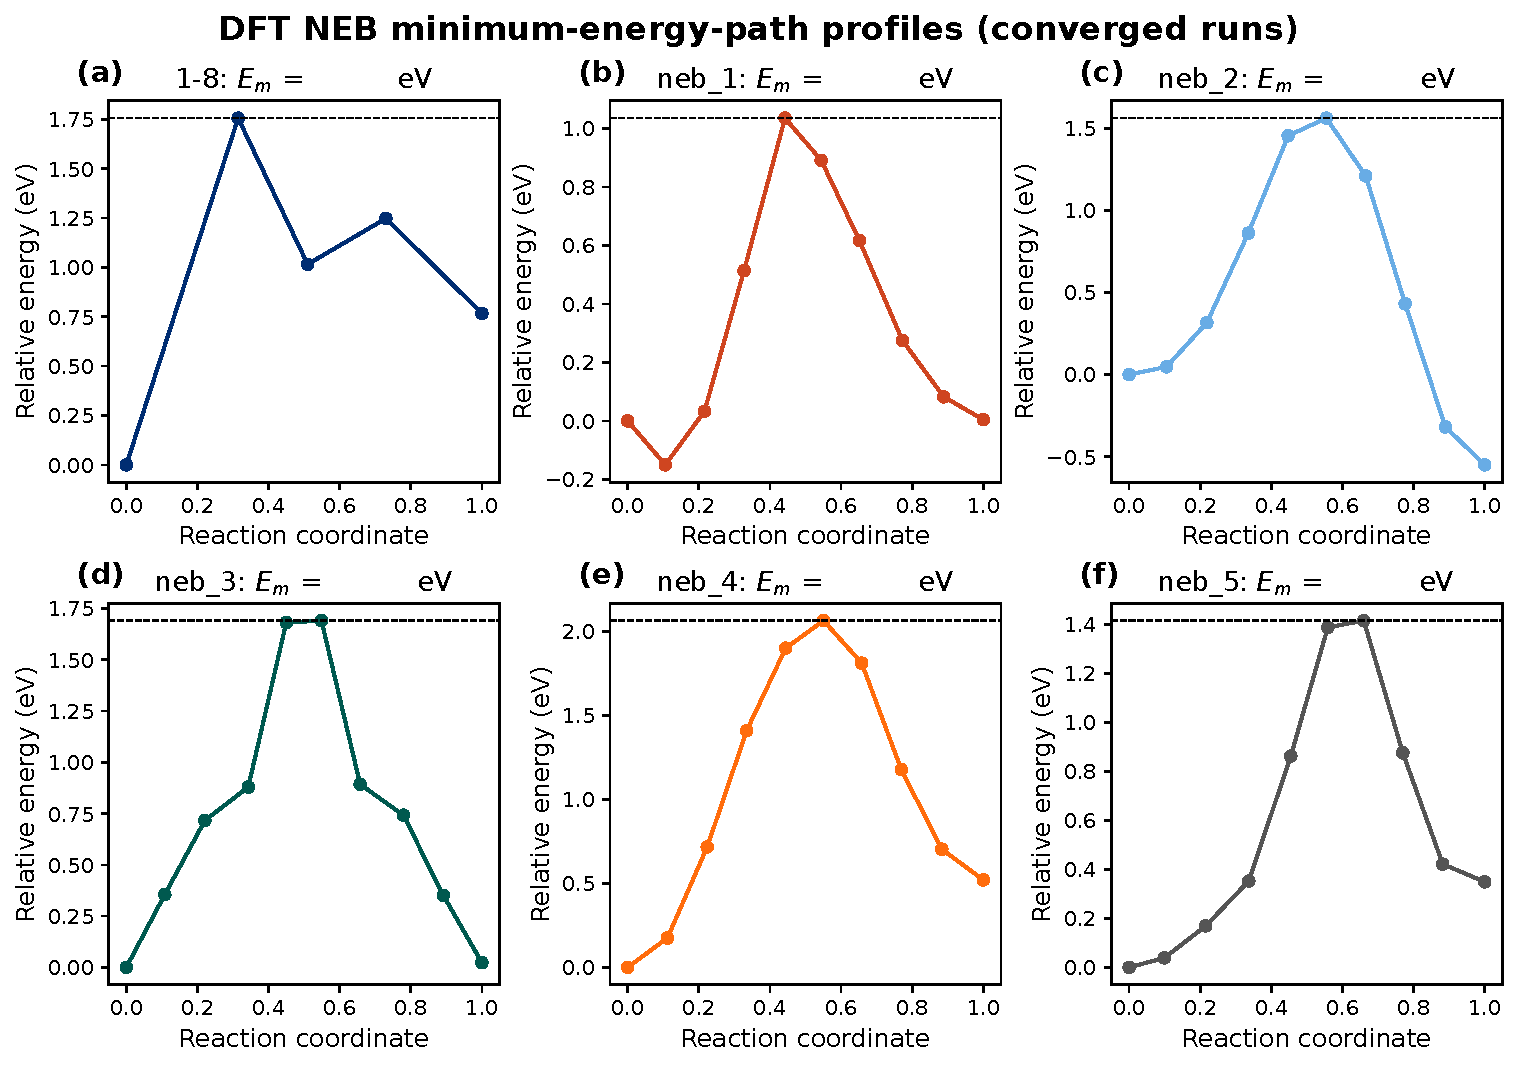
\includegraphics[width=\linewidth,height=0.42\textheight,keepaspectratio]{figure_pages/assets/fig_190.pdf}
\caption{Revision\textasciitilde{}1 article figure. This page shows the candidate output ``Figs dft neb mep profiles'' within the audited REV1-ARTICLE family. The panel identity, source scope, and current status are retained in the accompanying evidence matrix.}
\label{fig:candidate_190}
\end{figure}
\textbf{Results text draft.} The figure is already associated with the Revision\textasciitilde{}1 article structure and is presented here for page-level caption and prose review.
\textbf{Discussion and boundary.} Before final submission, confirm that the caption, Results text, and source ledger agree on the current audited values and exclusions.
\textbf{Article placement.} Proposed article location: Mapped by sn-article-final.tex or sn-article-SI.tex.
\textbf{Reviewer linkage:} overall status PARTIAL.
\begin{itemize}[leftmargin=1.4em,noitemsep]
\item \textbf{REV-A1 (PARTIAL):} Reconcile Fig. 3d fixed-geometry DFT-path scoring with SI Fig. S3 self-consistent MLFF-NEB, including pathway identity and the DFT reference. \emph{Completed:} The fixed-path versus self-relaxed operator distinction and the narrower model-reported-barrier wording are integrated. \emph{Still required:} Close the restartable QE path-1--4 convergence gate, preserve the final path/source metadata, and complete the SI Fig. S3 endpoint/checkpoint/optimizer/source audit before calling the quantitative reference final.
\end{itemize}
\textbf{Evidence pointers.}
\begin{itemize}[leftmargin=1.4em,noitemsep]
\item Caption/text source: \begingroup\scriptsize\url{paper/paper/revision1/benchmark_formalization.tex}\endgroup
\item Caption/text source: \begingroup\scriptsize\url{paper/paper/revision1/response_to_reviewers.log}\endgroup
\end{itemize}
\statusline{\textbf{Audit gap / next action:} Check figure source ledger and exact generator; some assets are compiled from older workflows}
\vfill
\clearpage
\section{FIG-191 --- Figs latent robustness}
\label{figpage:fig-191}
\textbf{Group:} REV1-ARTICLE\quad \textbf{Evidence chain:} traceable\quad \textbf{Status:} publication
\begin{figure}[H]
\centering
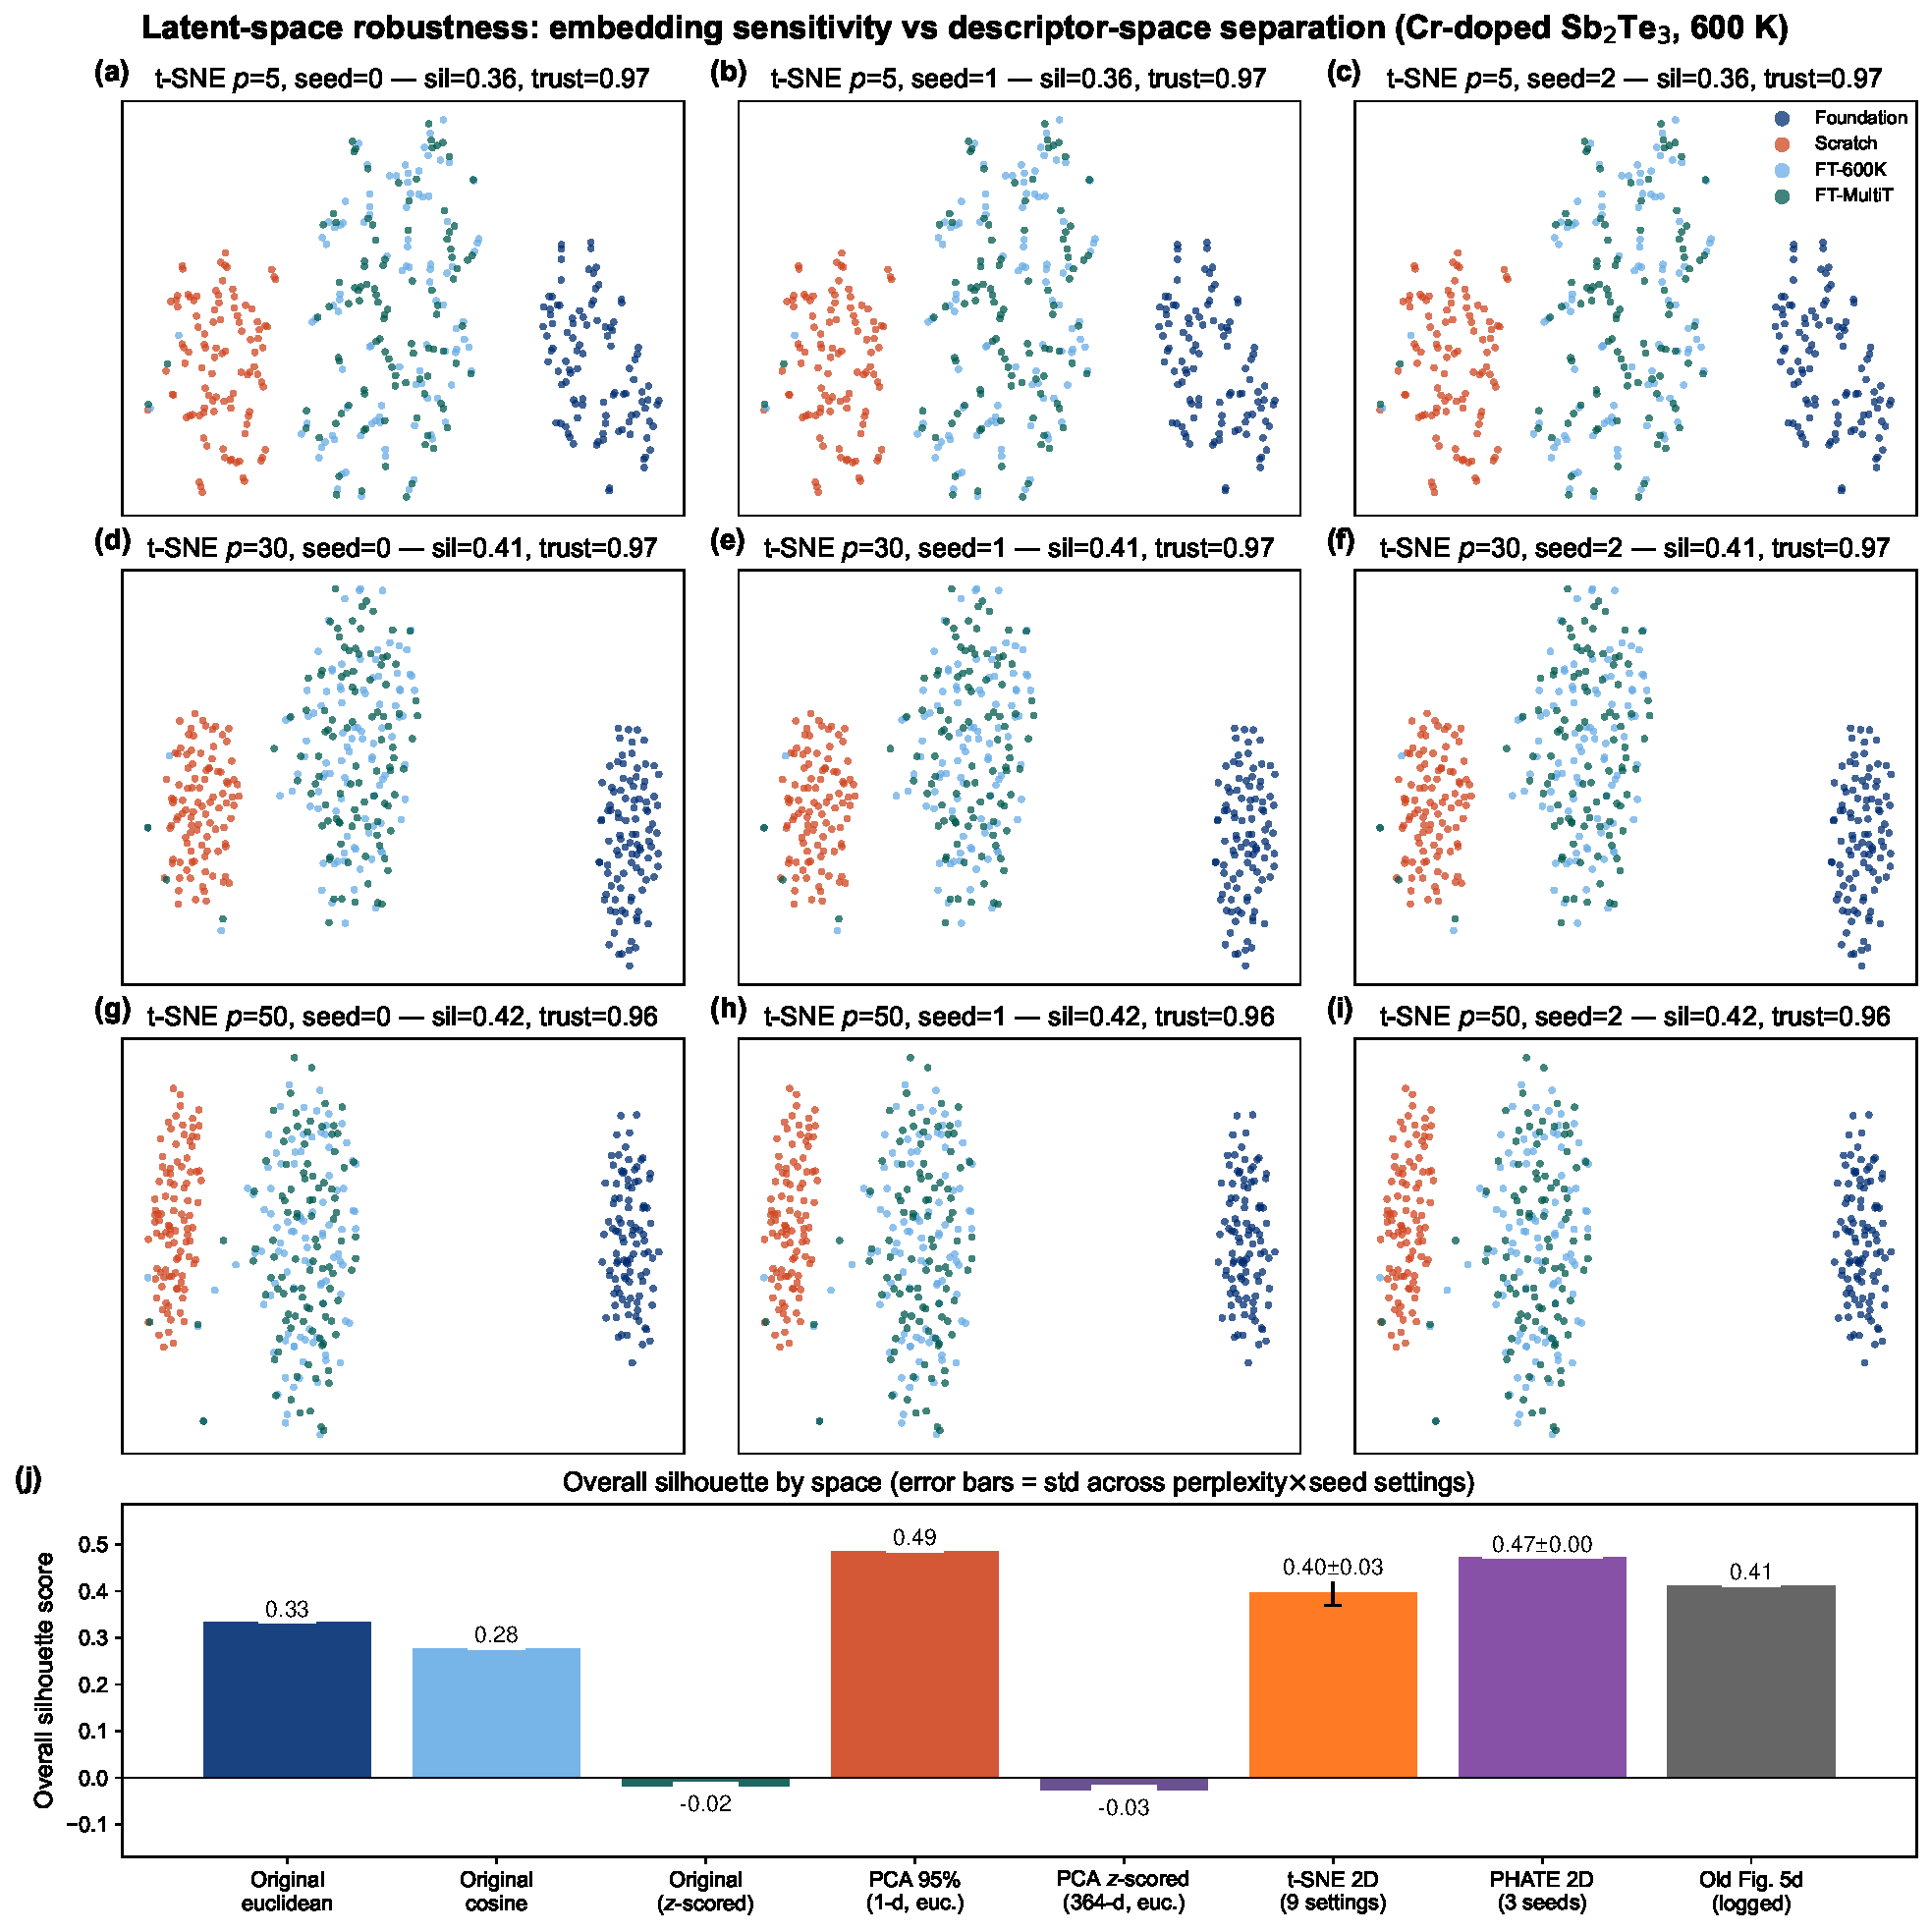
\includegraphics[width=\linewidth,height=0.42\textheight,keepaspectratio]{figure_pages/assets/fig_191.pdf}
\caption{Revision\textasciitilde{}1 article figure. This page shows the candidate output ``Figs latent robustness'' within the audited REV1-ARTICLE family. The panel identity, source scope, and current status are retained in the accompanying evidence matrix.}
\label{fig:candidate_191}
\end{figure}
\textbf{Results text draft.} The figure is already associated with the Revision\textasciitilde{}1 article structure and is presented here for page-level caption and prose review.
\textbf{Discussion and boundary.} Before final submission, confirm that the caption, Results text, and source ledger agree on the current audited values and exclusions.
\textbf{Article placement.} Proposed article location: Mapped by sn-article-final.tex or sn-article-SI.tex.
\textbf{Reviewer linkage:} overall status PARTIAL.
\begin{itemize}[leftmargin=1.4em,noitemsep]
\item \textbf{REV-A6 (PARTIAL):} Soften t-SNE/PHATE and SHAP interpretation claims and add projection/original-space and surrogate-fidelity checks. \emph{Completed:} Projection sensitivity, original-descriptor-space separation, and per-model cross-validated surrogate R2 are available; the text is scoped to descriptive/surrogate evidence. \emph{Still required:} A direct MACE Cr-Cr perturbation test remains pending if a causal claim about the dominant feature is desired; otherwise retain the surrogate-scoped wording.
\item \textbf{REV-C11 (DONE):} Compute separability in the original/high-dimensional descriptor space rather than only on a 2D embedding. \emph{Completed:} Original-space metrics and projection-sensitivity checks are available; embedding scores are retained only as descriptive baselines. \emph{Still required:} No new numerical figure is required; preserve the feature-space definition and scaling sensitivity in the caption/methods.
\item \textbf{REV-C12 (DONE):} Remove the always-zero force-sensitivity feature stub from the latent analysis. \emph{Completed:} The inactive channel was removed and no unsupported force-sensitivity claim is made. \emph{Still required:} No additional figure evidence is required unless a genuine finite-difference force-sensitivity analysis is later added.
\end{itemize}
\textbf{Evidence pointers.}
\begin{itemize}[leftmargin=1.4em,noitemsep]
\item Caption/text source: \begingroup\scriptsize\url{paper/paper/revision1/benchmark_formalization.tex}\endgroup
\item Caption/text source: \begingroup\scriptsize\url{paper/paper/revision1/response_to_reviewers.log}\endgroup
\end{itemize}
\statusline{\textbf{Audit gap / next action:} Check figure source ledger and exact generator; some assets are compiled from older workflows}
\vfill
\clearpage
\section{FIG-192 --- Figs neb pes local audit}
\label{figpage:fig-192}
\textbf{Group:} REV1-ARTICLE\quad \textbf{Evidence chain:} traceable\quad \textbf{Status:} publication;audit
\begin{figure}[H]
\centering
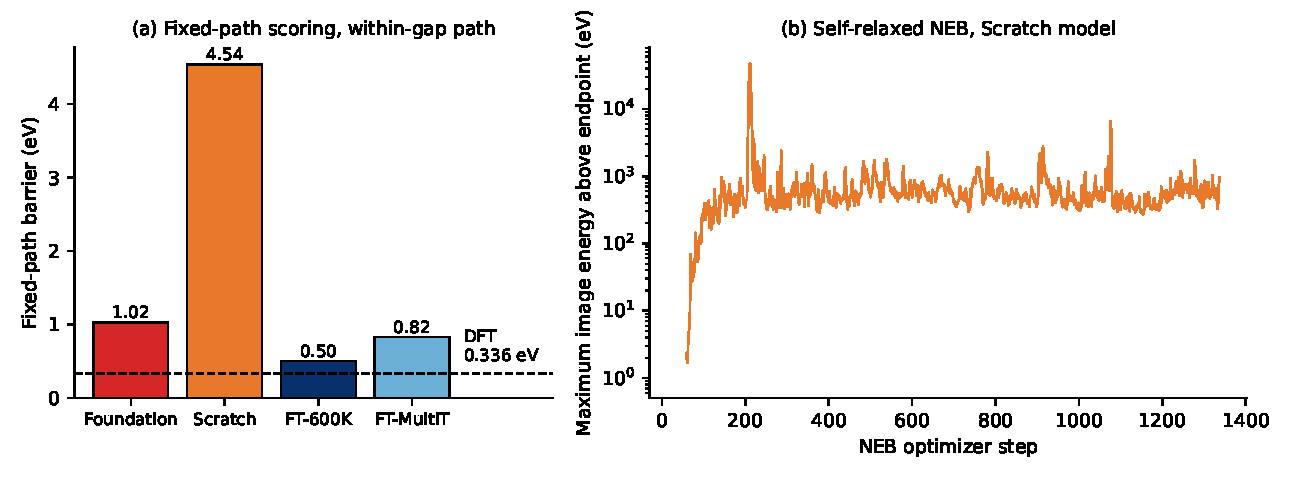
\includegraphics[width=\linewidth,height=0.42\textheight,keepaspectratio]{figure_pages/assets/fig_192_reader.pdf}
\caption{Revision\textasciitilde{}1 article figure. This page shows the candidate output ``Figs neb pes local audit'' within the audited REV1-ARTICLE family. The panel identity, source scope, and current status are retained in the accompanying evidence matrix.}
\label{fig:candidate_192}
\end{figure}
\textbf{Results text draft.} The figure is already associated with the Revision\textasciitilde{}1 article structure and is presented here for page-level caption and prose review.
\textbf{Discussion and boundary.} Before final submission, confirm that the caption, Results text, and source ledger agree on the current audited values and exclusions.
\textbf{Article placement.} Proposed article location: Mapped by sn-article-final.tex or sn-article-SI.tex.
\textbf{Reviewer linkage:} overall status PARTIAL.
\begin{itemize}[leftmargin=1.4em,noitemsep]
\item \textbf{REV-A1 (PARTIAL):} Reconcile Fig. 3d fixed-geometry DFT-path scoring with SI Fig. S3 self-consistent MLFF-NEB, including pathway identity and the DFT reference. \emph{Completed:} The fixed-path versus self-relaxed operator distinction and the narrower model-reported-barrier wording are integrated. \emph{Still required:} Close the restartable QE path-1--4 convergence gate, preserve the final path/source metadata, and complete the SI Fig. S3 endpoint/checkpoint/optimizer/source audit before calling the quantitative reference final.
\end{itemize}
\textbf{Evidence pointers.}
\begin{itemize}[leftmargin=1.4em,noitemsep]
\item Caption/text source: \begingroup\scriptsize\url{paper/paper/revision1/benchmark_formalization.tex}\endgroup
\item Caption/text source: \begingroup\scriptsize\url{paper/paper/revision1/response_to_reviewers.log}\endgroup
\end{itemize}
\statusline{\textbf{Audit gap / next action:} Check figure source ledger and exact generator; some assets are compiled from older workflows}
\vfill
\clearpage
\section{FIG-193 --- Fig md msd kappa revised}
\label{figpage:fig-193}
\textbf{Group:} REV1-ARTICLE\quad \textbf{Evidence chain:} traceable\quad \textbf{Status:} publication
\begin{figure}[H]
\centering
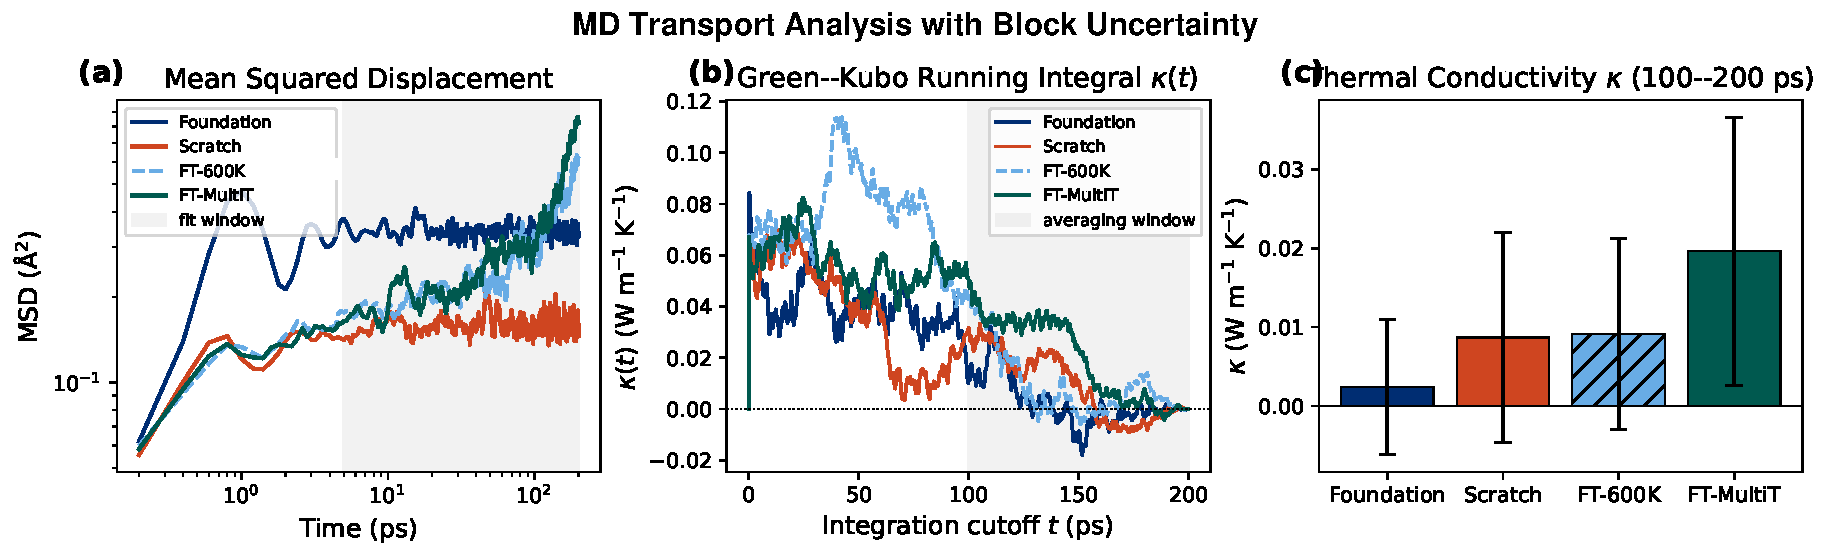
\includegraphics[width=\linewidth,height=0.42\textheight,keepaspectratio]{figure_pages/assets/fig_193_reader.pdf}
\caption{Revision\textasciitilde{}1 article figure. This page shows the candidate output ``Fig md msd kappa revised'' within the audited REV1-ARTICLE family. The panel identity, source scope, and current status are retained in the accompanying evidence matrix.}
\label{fig:candidate_193}
\end{figure}
\textbf{Results text draft.} The figure is already associated with the Revision\textasciitilde{}1 article structure and is presented here for page-level caption and prose review.
\textbf{Discussion and boundary.} Before final submission, confirm that the caption, Results text, and source ledger agree on the current audited values and exclusions.
\textbf{Article placement.} Proposed article location: Mapped by sn-article-final.tex or sn-article-SI.tex.
\textbf{Reviewer linkage:} overall status PENDING.
\begin{itemize}[leftmargin=1.4em,noitemsep]
\item \textbf{REV-C9 (PENDING):} Resolve the asymmetric FT-600K MD transport protocol and its effect on D and kappa. \emph{Completed:} Legacy FT-600K transport values are quarantined and excluded from ranking; the figure can document that boundary. \emph{Still required:} Run the corrected matched-protocol FT-600K long trajectory, block-average D/kappa, and close the multi-seed uncertainty before reporting a final transport comparison.
\end{itemize}
\textbf{Evidence pointers.}
\begin{itemize}[leftmargin=1.4em,noitemsep]
\item Caption/text source: \begingroup\scriptsize\url{paper/paper/revision1/benchmark_formalization.tex}\endgroup
\item Caption/text source: \begingroup\scriptsize\url{paper/paper/revision1/response_to_reviewers.log}\endgroup
\end{itemize}
\statusline{\textbf{Audit gap / next action:} Check figure source ledger and exact generator; some assets are compiled from older workflows}
\vfill
\clearpage
\section{FIG-194 --- Path 1 4 energy profiles corrected}
\label{figpage:fig-194}
\textbf{Group:} REV1-FOUNDATION\quad \textbf{Evidence chain:} traceable\quad \textbf{Status:} publication;comparison
\begin{figure}[H]
\centering
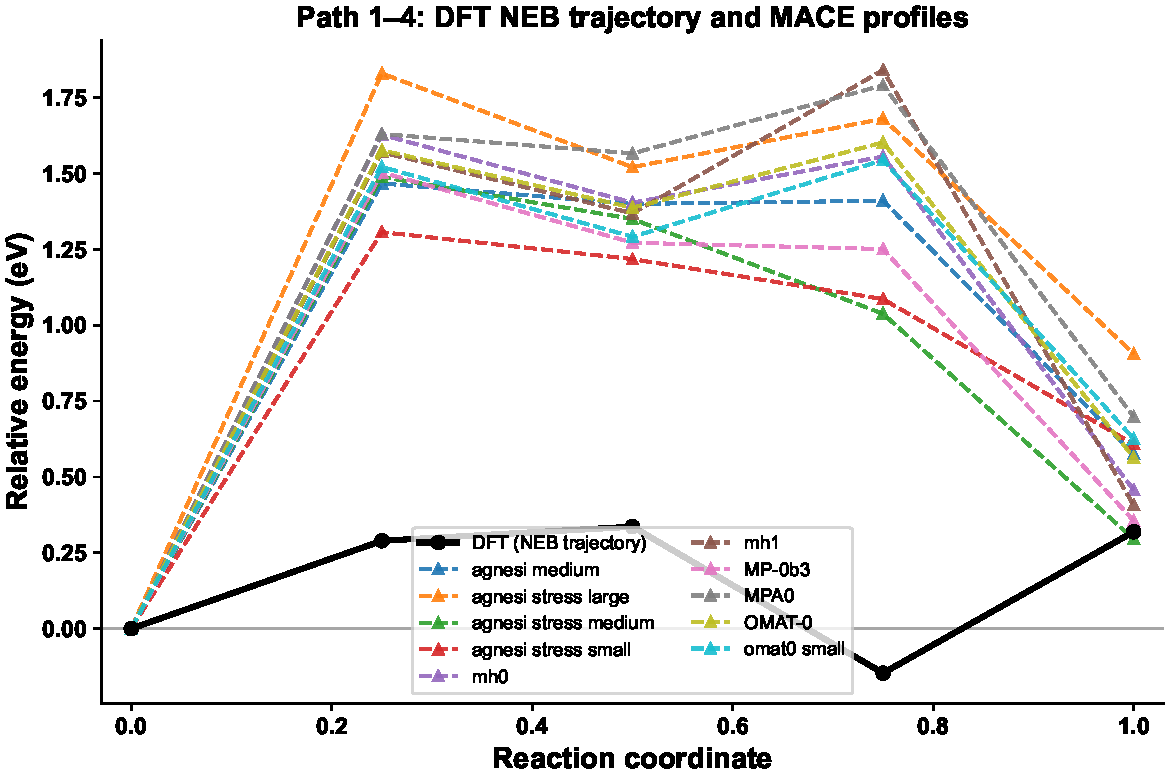
\includegraphics[width=\linewidth,height=0.42\textheight,keepaspectratio]{figure_pages/assets/fig_194.pdf}
\caption{Revision\textasciitilde{}1 foundation-model pathway or representation diagnostic. This page shows the candidate output ``Path 1 4 energy profiles corrected'' within the audited REV1-FOUNDATION family. The panel identity, source scope, and current status are retained in the accompanying evidence matrix.}
\label{fig:candidate_194}
\end{figure}
\textbf{Results text draft.} The figure compares the declared foundation-model families or representations under the audited pathway/descriptor scope. Family variation is kept distinct from training-seed uncertainty.
\textbf{Discussion and boundary.} Use for the corresponding SI or Results discussion only after the provisional reference and descriptor-space limitations are stated.
\textbf{Article placement.} Proposed article location: SI Detailed Migration Pathway Analysis / In-Gap Diffusion.
\textbf{Reviewer linkage:} overall status PARTIAL.
\begin{itemize}[leftmargin=1.4em,noitemsep]
\item \textbf{REV-A1 (PARTIAL):} Reconcile Fig. 3d fixed-geometry DFT-path scoring with SI Fig. S3 self-consistent MLFF-NEB, including pathway identity and the DFT reference. \emph{Completed:} The fixed-path versus self-relaxed operator distinction and the narrower model-reported-barrier wording are integrated. \emph{Still required:} Close the restartable QE path-1--4 convergence gate, preserve the final path/source metadata, and complete the SI Fig. S3 endpoint/checkpoint/optimizer/source audit before calling the quantitative reference final.
\end{itemize}
\textbf{Evidence pointers.}
No data/script/text candidate was recorded in the matrix; resolve this gap before manuscript promotion.
\statusline{\textbf{Audit gap / next action:} DFT path is provisional; no self-relaxed NEB interpretation}
\vfill
\clearpage
\section{FIG-195 --- Path 1 4 energy profiles family aggregated}
\label{figpage:fig-195}
\textbf{Group:} REV1-FOUNDATION\quad \textbf{Evidence chain:} traceable\quad \textbf{Status:} publication;comparison
\begin{figure}[H]
\centering
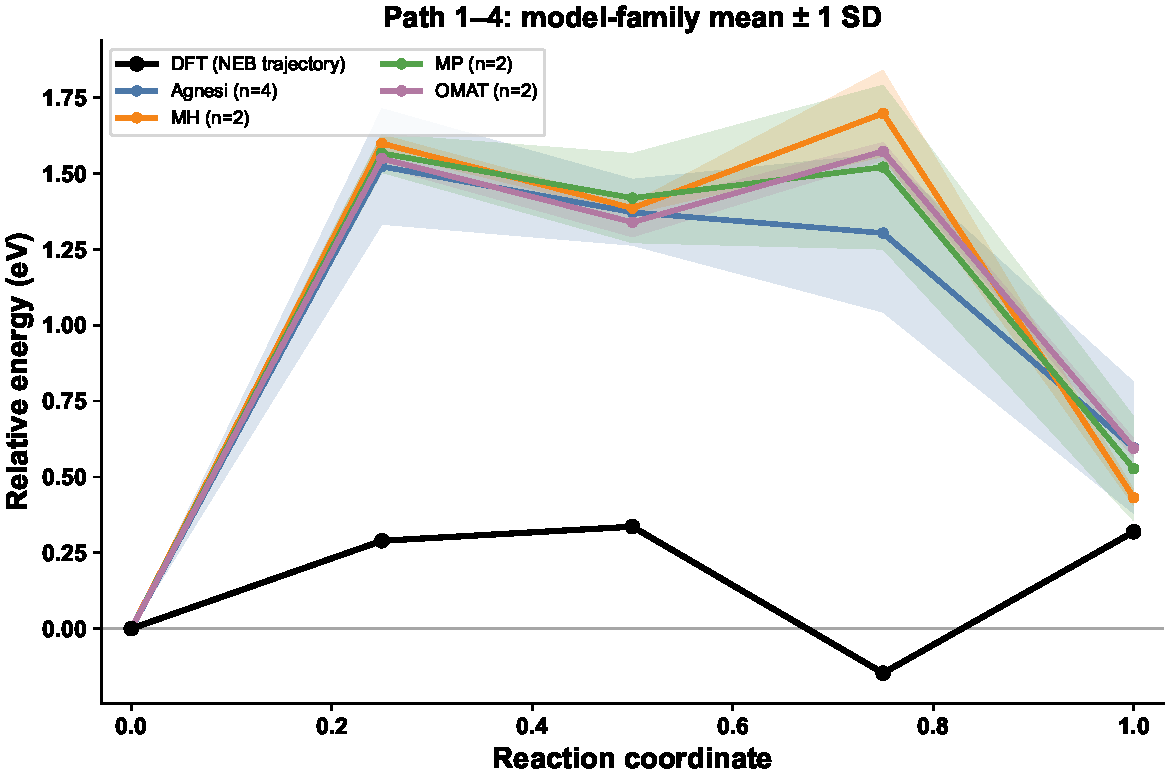
\includegraphics[width=\linewidth,height=0.42\textheight,keepaspectratio]{figure_pages/assets/fig_195.pdf}
\caption{Revision\textasciitilde{}1 foundation-model pathway or representation diagnostic. This page shows the candidate output ``Path 1 4 energy profiles family aggregated'' within the audited REV1-FOUNDATION family. The panel identity, source scope, and current status are retained in the accompanying evidence matrix.}
\label{fig:candidate_195}
\end{figure}
\textbf{Results text draft.} The figure compares the declared foundation-model families or representations under the audited pathway/descriptor scope. Family variation is kept distinct from training-seed uncertainty.
\textbf{Discussion and boundary.} Use for the corresponding SI or Results discussion only after the provisional reference and descriptor-space limitations are stated.
\textbf{Article placement.} Proposed article location: SI Detailed Migration Pathway Analysis / In-Gap Diffusion.
\textbf{Reviewer linkage:} overall status PARTIAL.
\begin{itemize}[leftmargin=1.4em,noitemsep]
\item \textbf{REV-A1 (PARTIAL):} Reconcile Fig. 3d fixed-geometry DFT-path scoring with SI Fig. S3 self-consistent MLFF-NEB, including pathway identity and the DFT reference. \emph{Completed:} The fixed-path versus self-relaxed operator distinction and the narrower model-reported-barrier wording are integrated. \emph{Still required:} Close the restartable QE path-1--4 convergence gate, preserve the final path/source metadata, and complete the SI Fig. S3 endpoint/checkpoint/optimizer/source audit before calling the quantitative reference final.
\end{itemize}
\textbf{Evidence pointers.}
No data/script/text candidate was recorded in the matrix; resolve this gap before manuscript promotion.
\statusline{\textbf{Audit gap / next action:} DFT path is provisional; no self-relaxed NEB interpretation}
\vfill
\clearpage
\section{FIG-196 --- Response to reviewers}
\label{figpage:fig-196}
\textbf{Group:} PAPER-OTHER\quad \textbf{Evidence chain:} partial\quad \textbf{Status:} publication
\begin{figure}[H]
\centering
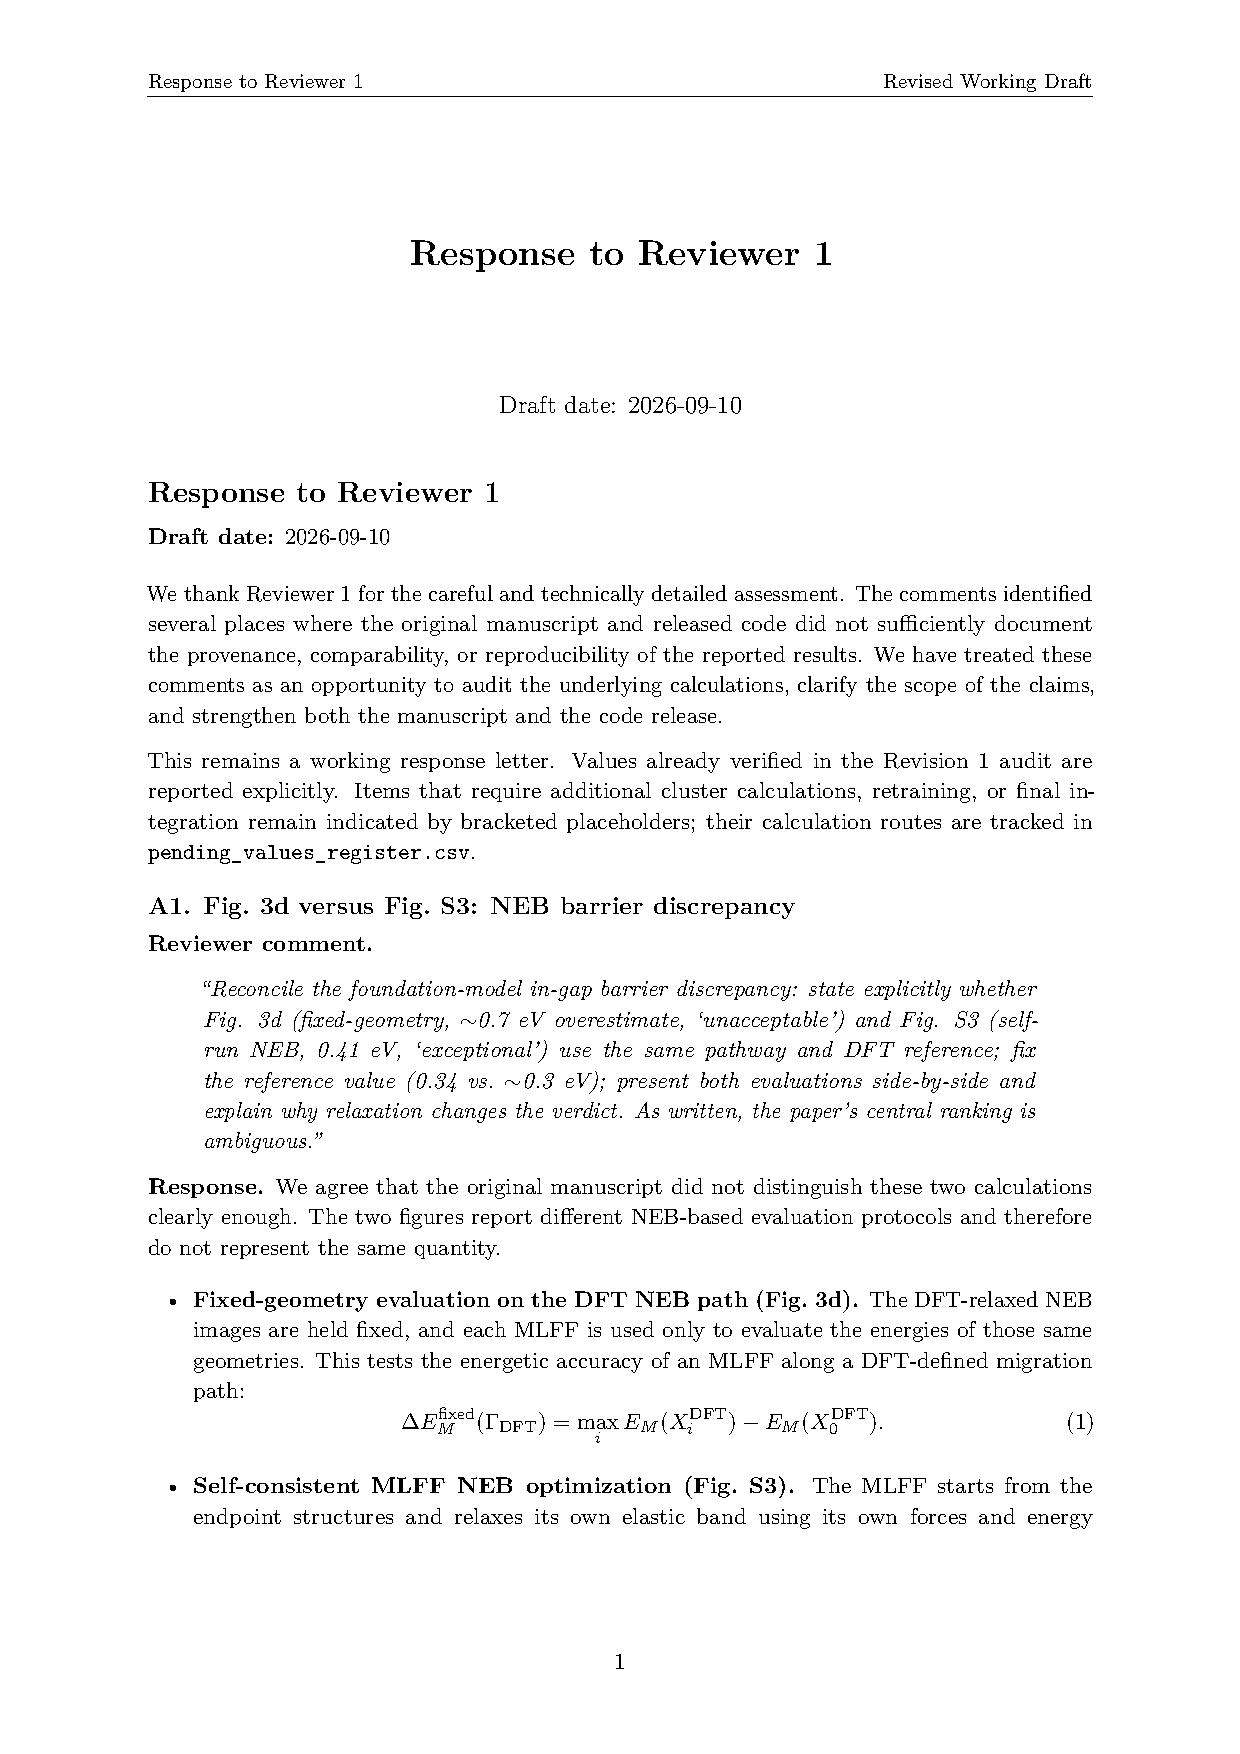
\includegraphics[width=\linewidth,height=0.42\textheight,keepaspectratio]{figure_pages/assets/fig_196.pdf}
\caption{Other paper/repro figure candidate. This page shows the candidate output ``Response to reviewers'' within the audited PAPER-OTHER family. The panel identity, source scope, and current status are retained in the accompanying evidence matrix.}
\label{fig:candidate_196}
\end{figure}
\textbf{Results text draft.} This candidate is retained because it is referenced by the paper/repro project but does not yet belong to a fully mapped primary group. Its data and manuscript linkage are listed on this page.
\textbf{Discussion and boundary.} Resolve the article label and evidence gap before promoting it into the main text or SI.
\textbf{Article placement.} Proposed article location: unmapped.
\textbf{Reviewer linkage:} overall status NO\_DIRECT\_REVIEWER\_FIGURE\_LINK.
No direct reviewer-response figure linkage was identified; this page is retained for scientific/article audit rather than as a direct reviewer response.
\textbf{Evidence pointers.}
\begin{itemize}[leftmargin=1.4em,noitemsep]
\item Caption/text source: \begingroup\scriptsize\url{paper/paper/response_to_reviewers.log}\endgroup
\item Caption/text source: \begingroup\scriptsize\url{paper/paper/response_to_reviewers.out}\endgroup
\end{itemize}
\statusline{\textbf{Audit gap / next action:} Needs manual family assignment}
\vfill
\clearpage
\section{FIG-197 --- Sn article si}
\label{figpage:fig-197}
\textbf{Group:} REV1-COMPILED\quad \textbf{Evidence chain:} compiled document\quad \textbf{Status:} publication
\begin{figure}[H]
\centering
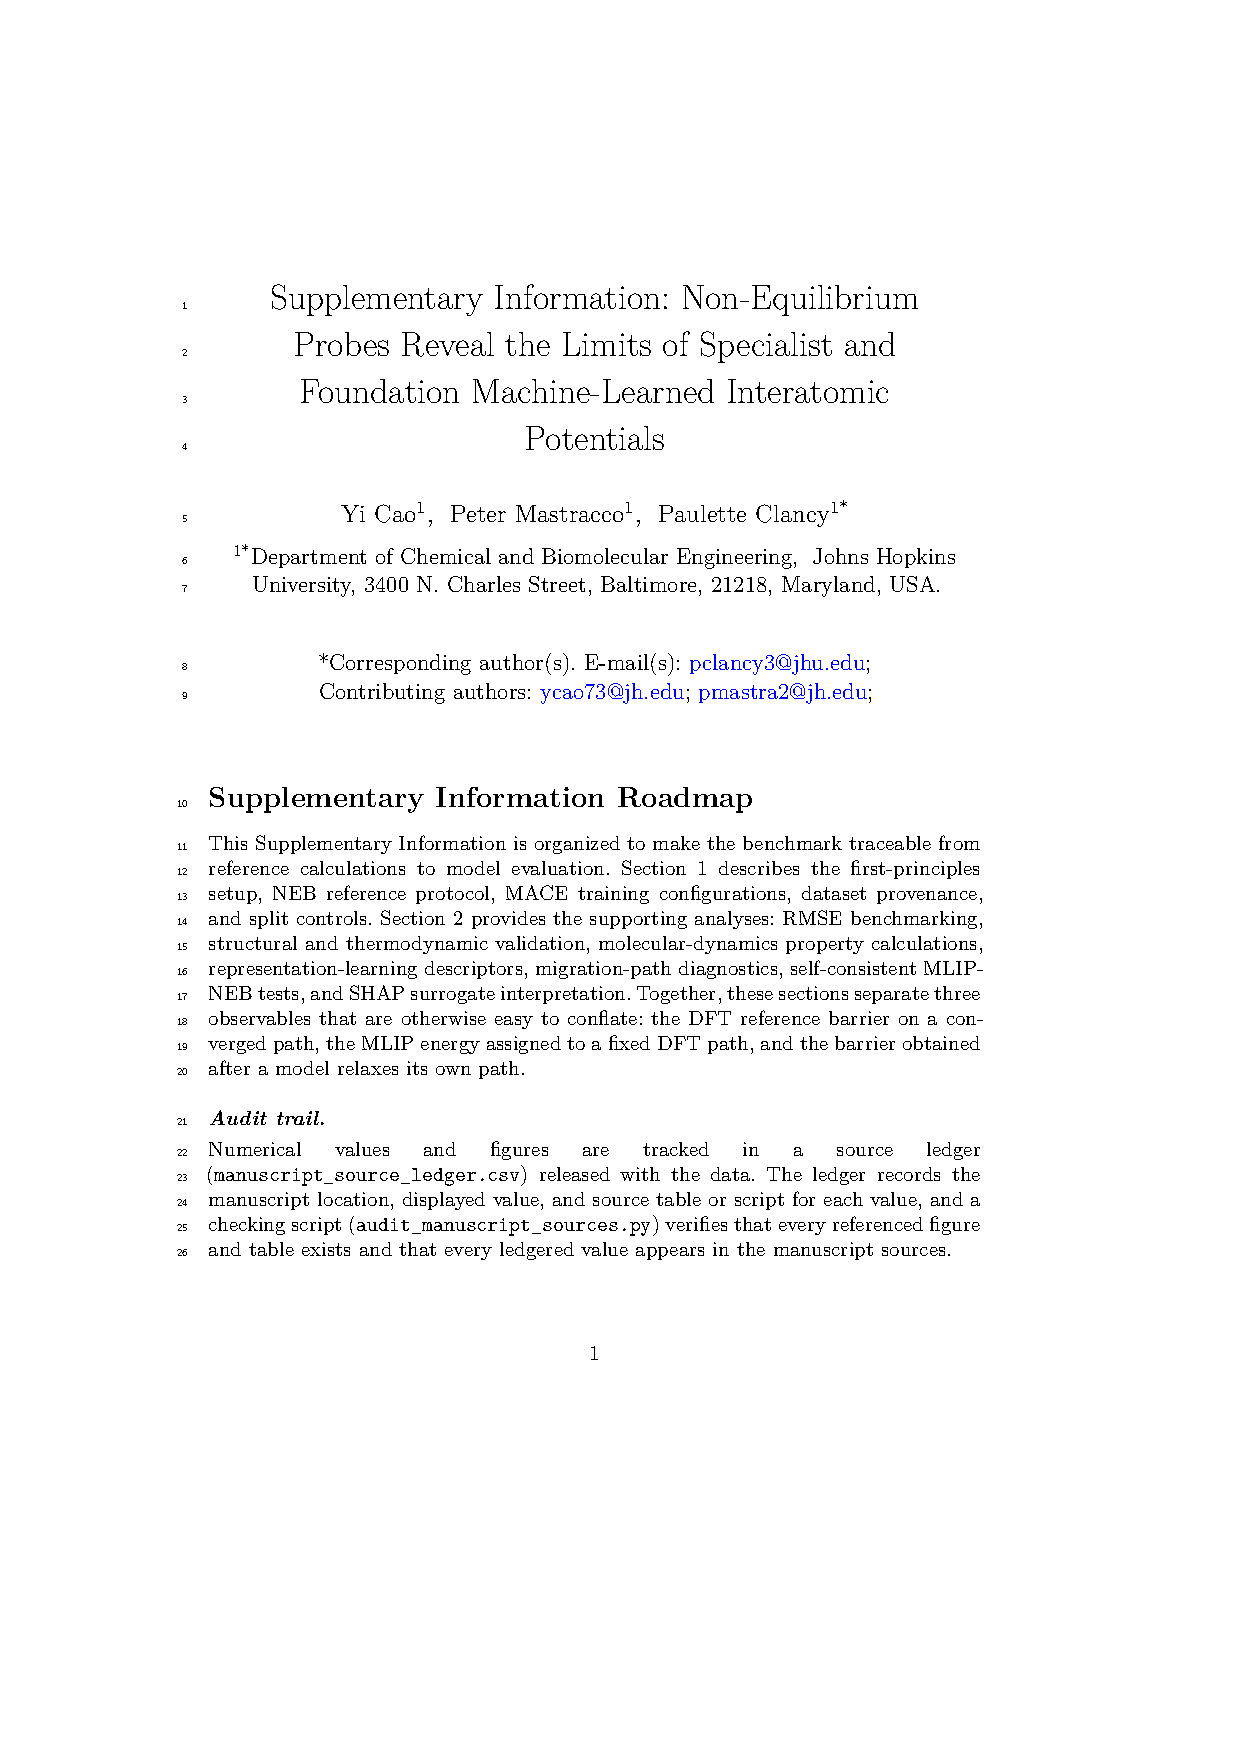
\includegraphics[width=\linewidth,height=0.42\textheight,keepaspectratio]{figure_pages/assets/fig_197_reader.pdf}
\caption{Compiled revision\textasciitilde{}1 manuscript figure/document artifact. This page shows the candidate output ``Sn article si'' within the audited REV1-COMPILED family. The panel identity, source scope, and current status are retained in the accompanying evidence matrix.}
\label{fig:candidate_197}
\end{figure}
\textbf{Results text draft.} This page preserves the compiled Revision\textasciitilde{}1 artifact for visual reconciliation against the editable source and source ledger.
\textbf{Discussion and boundary.} The compiled artifact is not an independent data source; use the editable figure and its reproducible chain for final claims.
\textbf{Article placement.} Proposed article location: Entire manuscript/SI.
\textbf{Reviewer linkage:} overall status NO\_DIRECT\_REVIEWER\_FIGURE\_LINK.
No direct reviewer-response figure linkage was identified; this page is retained for scientific/article audit rather than as a direct reviewer response.
\textbf{Evidence pointers.}
\begin{itemize}[leftmargin=1.4em,noitemsep]
\item Caption/text source: \begingroup\scriptsize\url{paper/paper/response_to_reviewers.log}\endgroup
\item Caption/text source: \begingroup\scriptsize\url{paper/paper/response_to_reviewers.out}\endgroup
\end{itemize}
\statusline{\textbf{Audit gap / next action:} Not an independent figure; audit included figure assets instead}
\vfill
\clearpage
\section{FIG-198 --- Sn article final}
\label{figpage:fig-198}
\textbf{Group:} REV1-COMPILED\quad \textbf{Evidence chain:} compiled document\quad \textbf{Status:} publication
\begin{figure}[H]
\centering
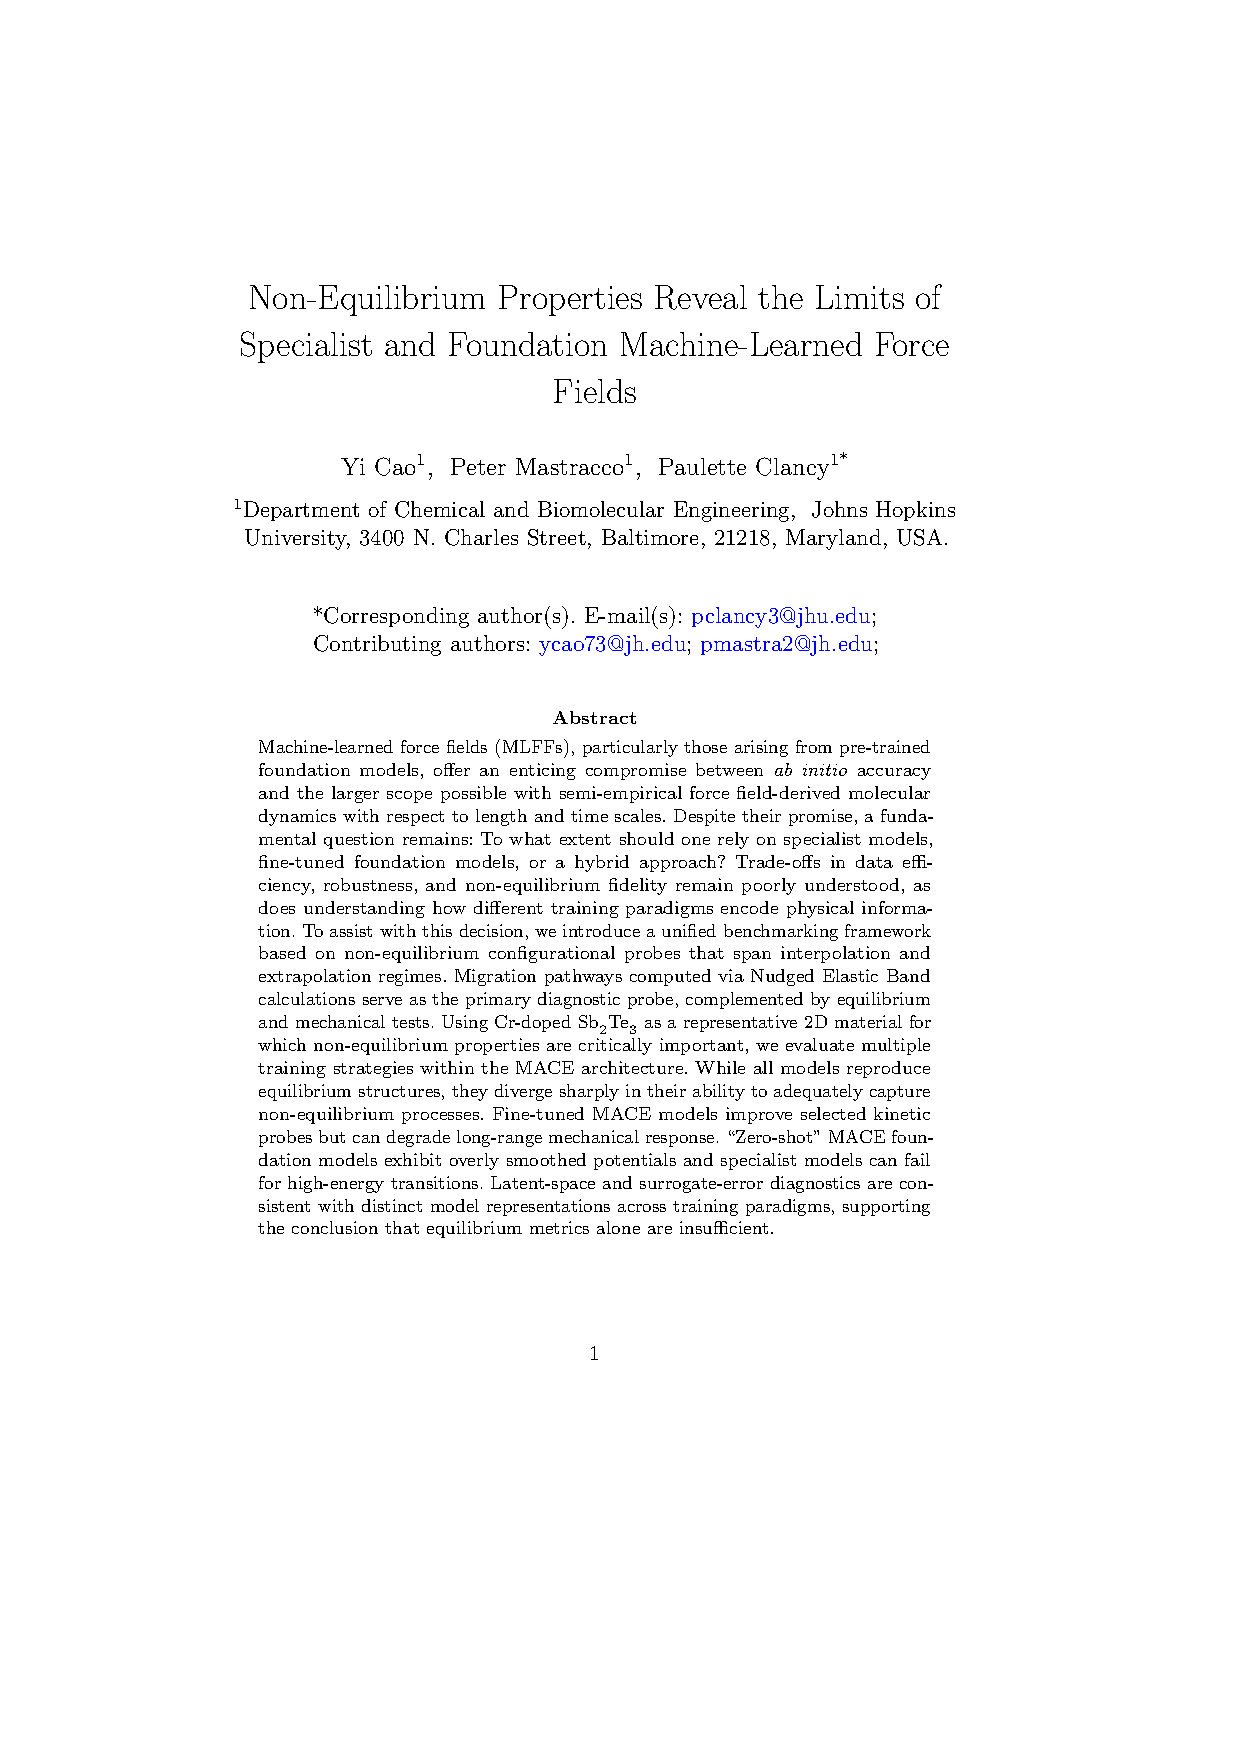
\includegraphics[width=\linewidth,height=0.42\textheight,keepaspectratio]{figure_pages/assets/fig_198.pdf}
\caption{Compiled revision\textasciitilde{}1 manuscript figure/document artifact. This page shows the candidate output ``Sn article final'' within the audited REV1-COMPILED family. The panel identity, source scope, and current status are retained in the accompanying evidence matrix.}
\label{fig:candidate_198}
\end{figure}
\textbf{Results text draft.} This page preserves the compiled Revision\textasciitilde{}1 artifact for visual reconciliation against the editable source and source ledger.
\textbf{Discussion and boundary.} The compiled artifact is not an independent data source; use the editable figure and its reproducible chain for final claims.
\textbf{Article placement.} Proposed article location: Entire manuscript/SI.
\textbf{Reviewer linkage:} overall status NO\_DIRECT\_REVIEWER\_FIGURE\_LINK.
No direct reviewer-response figure linkage was identified; this page is retained for scientific/article audit rather than as a direct reviewer response.
\textbf{Evidence pointers.}
\begin{itemize}[leftmargin=1.4em,noitemsep]
\item Caption/text source: \begingroup\scriptsize\url{paper/paper/response_to_reviewers.log}\endgroup
\item Caption/text source: \begingroup\scriptsize\url{paper/paper/response_to_reviewers.out}\endgroup
\end{itemize}
\statusline{\textbf{Audit gap / next action:} Not an independent figure; audit included figure assets instead}
\vfill
\clearpage
\section{FIG-199 --- Sn article si}
\label{figpage:fig-199}
\textbf{Group:} COMPILED-DOCUMENT\quad \textbf{Evidence chain:} compiled document\quad \textbf{Status:} publication
\begin{figure}[H]
\centering
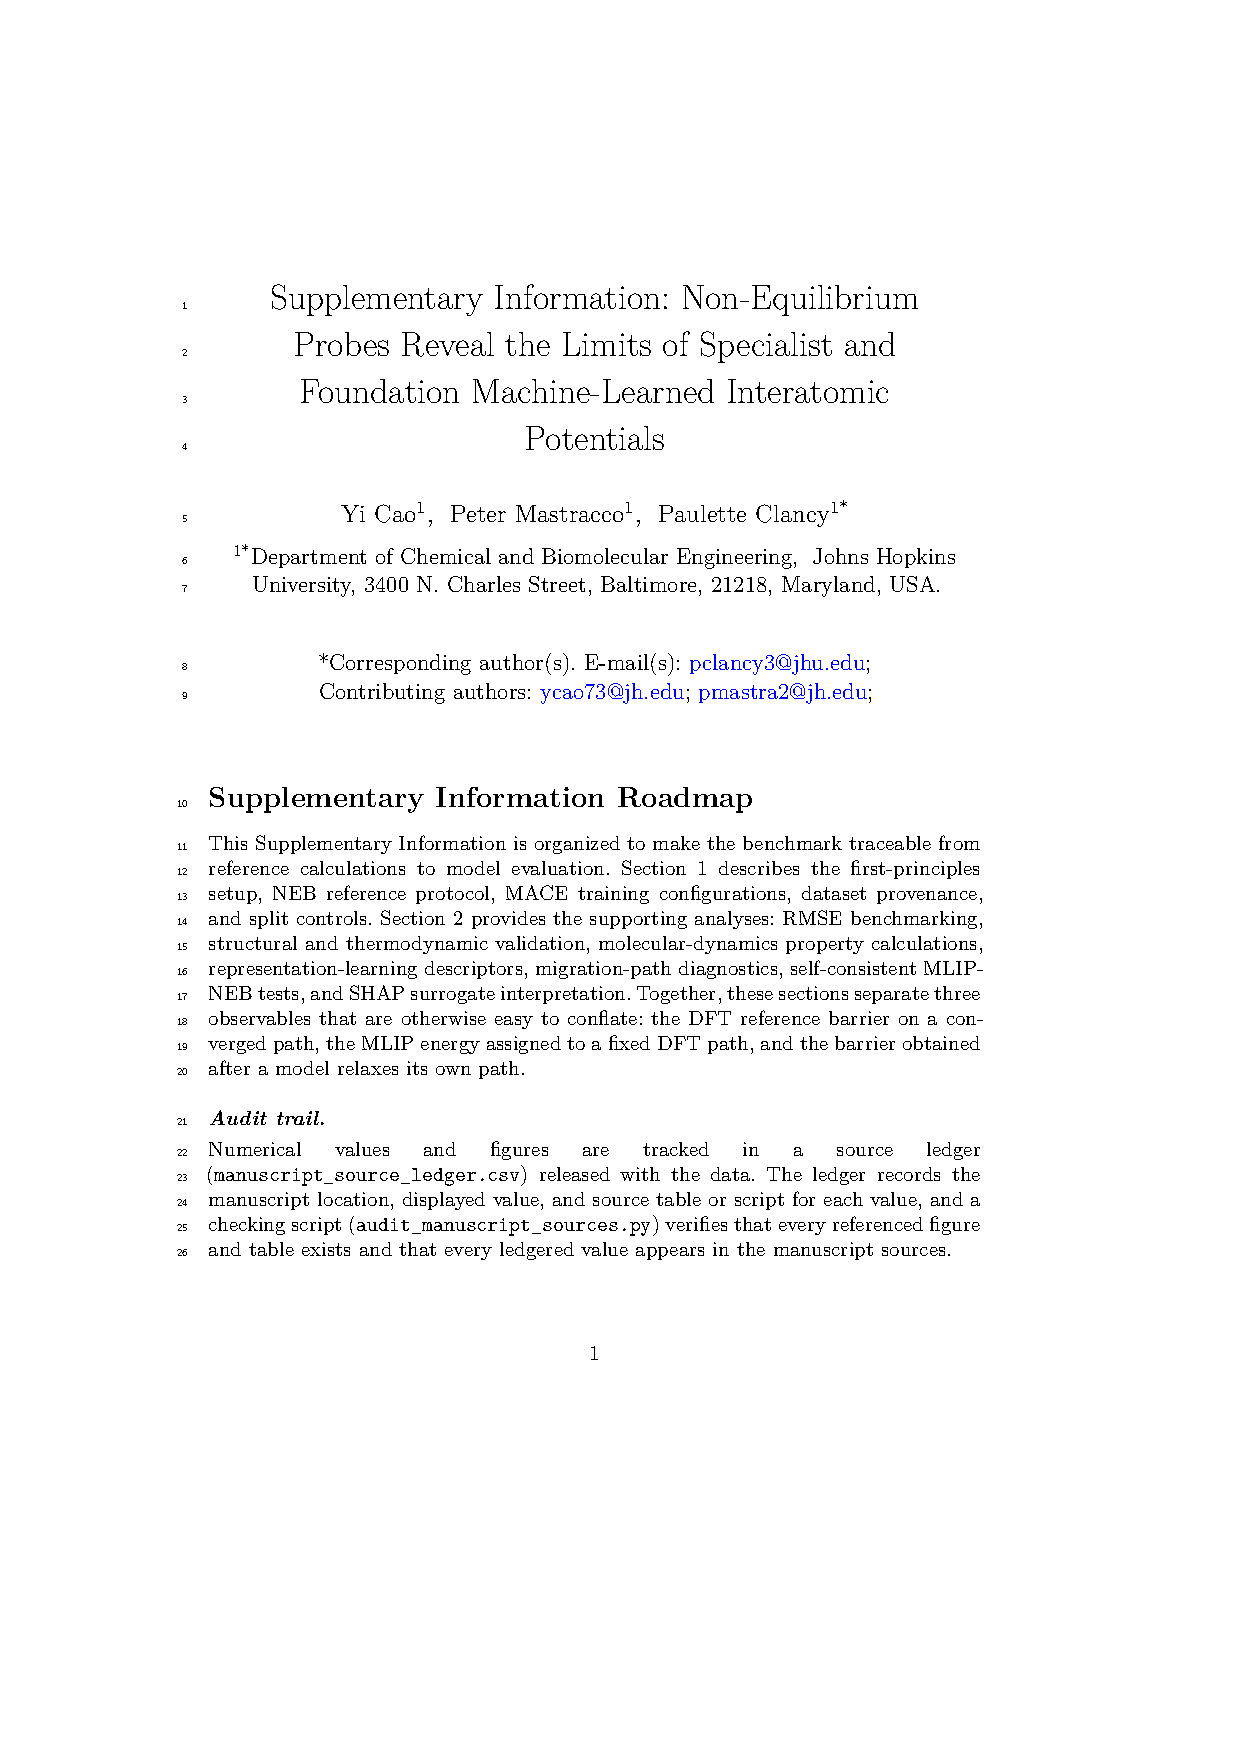
\includegraphics[width=\linewidth,height=0.42\textheight,keepaspectratio]{figure_pages/assets/fig_199_reader.pdf}
\caption{Compiled manuscript or response artifact retained as document-level evidence. This page shows the candidate output ``Sn article si'' within the audited COMPILED-DOCUMENT family. The panel identity, source scope, and current status are retained in the accompanying evidence matrix.}
\label{fig:candidate_199}
\end{figure}
\textbf{Results text draft.} This entry is a compiled document rather than an independent scientific figure. It is retained because it may contain figure captions, rendered panels, or response language that must be reconciled with the source ledger.
\textbf{Discussion and boundary.} Use only as document provenance; cite the underlying figure and reproducible source chain for scientific claims.
\textbf{Article placement.} Proposed article location: Response or manuscript.
\textbf{Reviewer linkage:} overall status NO\_DIRECT\_REVIEWER\_FIGURE\_LINK.
No direct reviewer-response figure linkage was identified; this page is retained for scientific/article audit rather than as a direct reviewer response.
\textbf{Evidence pointers.}
\begin{itemize}[leftmargin=1.4em,noitemsep]
\item Caption/text source: \begingroup\scriptsize\url{paper/README.md}\endgroup
\item Caption/text source: \begingroup\scriptsize\url{paper/paper/response_to_reviewers.log}\endgroup
\end{itemize}
\statusline{\textbf{Audit gap / next action:} Not an independent figure}
\vfill
\clearpage
\section{FIG-200 --- Sn article final}
\label{figpage:fig-200}
\textbf{Group:} COMPILED-DOCUMENT\quad \textbf{Evidence chain:} compiled document\quad \textbf{Status:} publication
\begin{figure}[H]
\centering
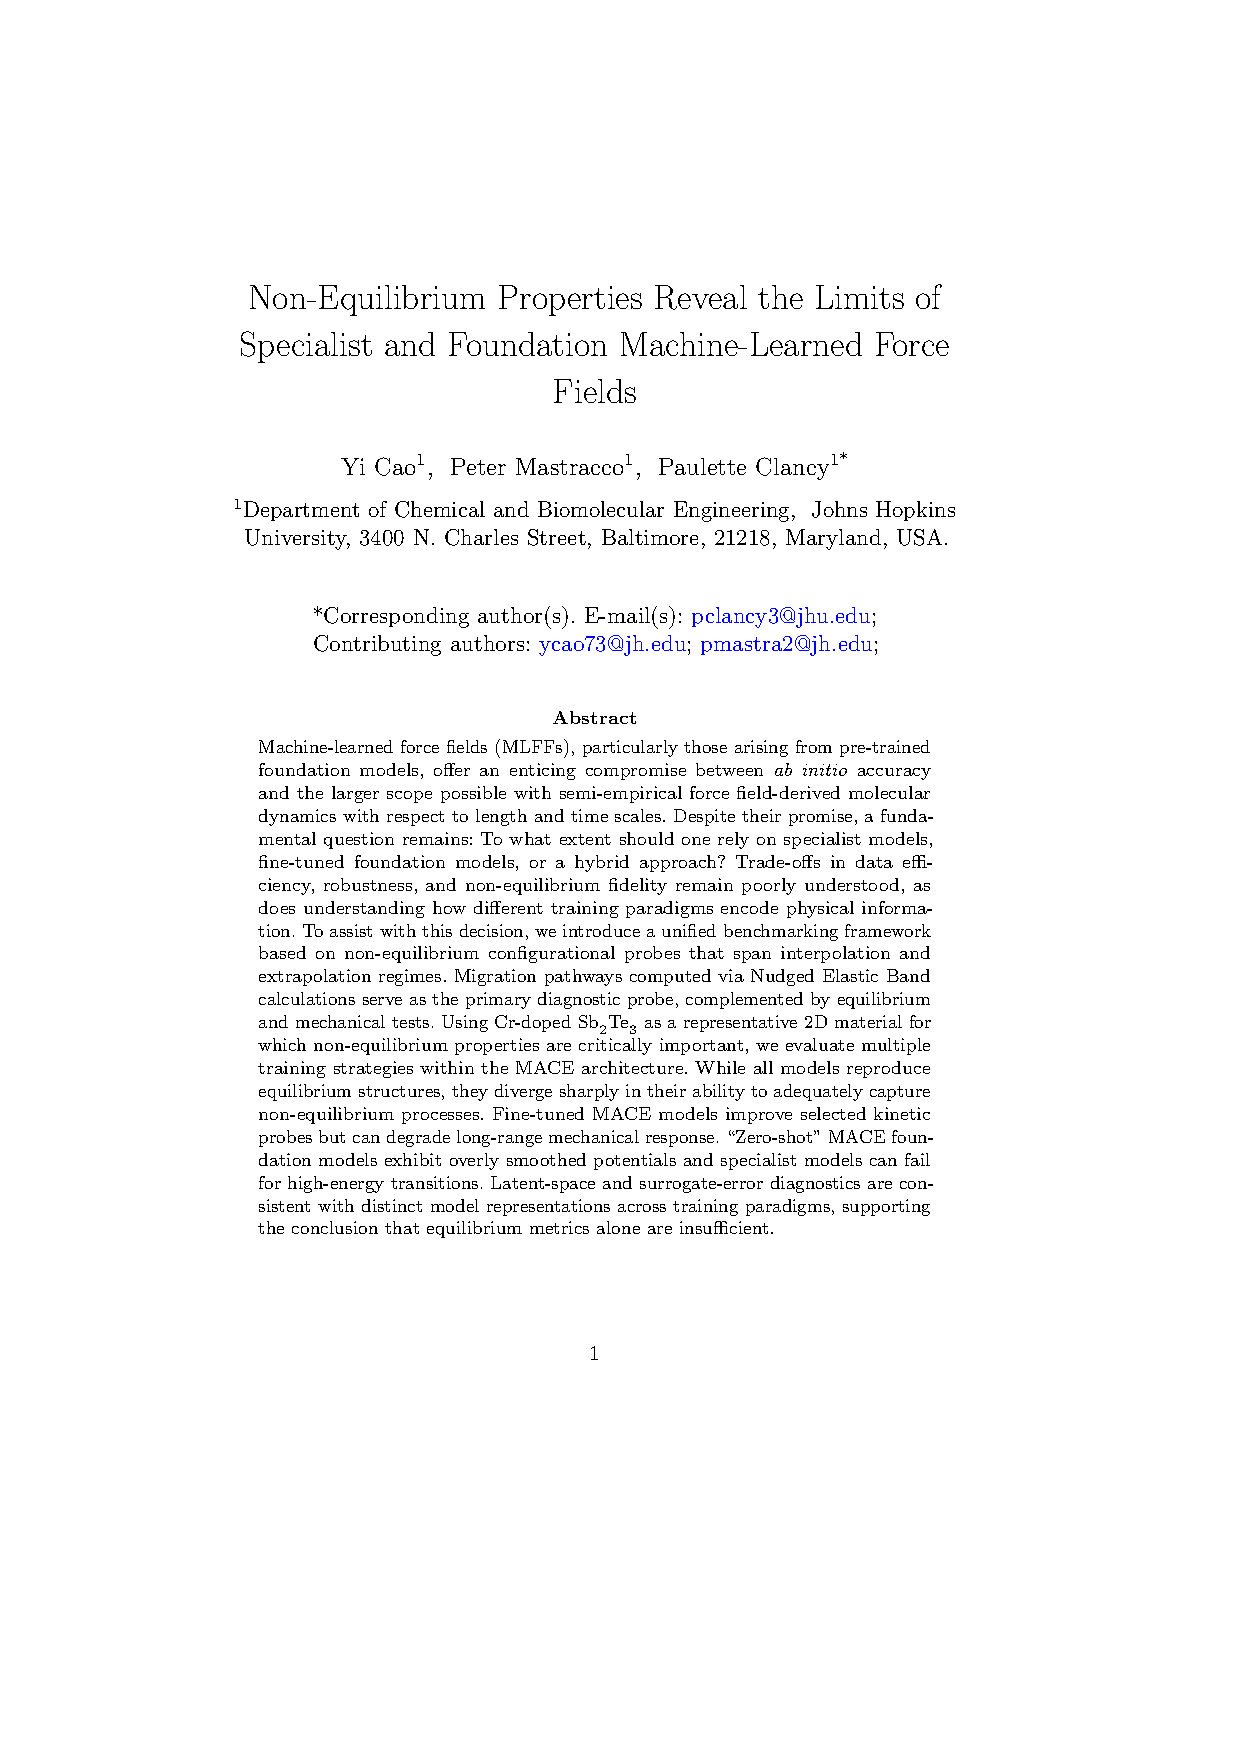
\includegraphics[width=\linewidth,height=0.42\textheight,keepaspectratio]{figure_pages/assets/fig_200.pdf}
\caption{Compiled manuscript or response artifact retained as document-level evidence. This page shows the candidate output ``Sn article final'' within the audited COMPILED-DOCUMENT family. The panel identity, source scope, and current status are retained in the accompanying evidence matrix.}
\label{fig:candidate_200}
\end{figure}
\textbf{Results text draft.} This entry is a compiled document rather than an independent scientific figure. It is retained because it may contain figure captions, rendered panels, or response language that must be reconciled with the source ledger.
\textbf{Discussion and boundary.} Use only as document provenance; cite the underlying figure and reproducible source chain for scientific claims.
\textbf{Article placement.} Proposed article location: Response or manuscript.
\textbf{Reviewer linkage:} overall status NO\_DIRECT\_REVIEWER\_FIGURE\_LINK.
No direct reviewer-response figure linkage was identified; this page is retained for scientific/article audit rather than as a direct reviewer response.
\textbf{Evidence pointers.}
\begin{itemize}[leftmargin=1.4em,noitemsep]
\item Caption/text source: \begingroup\scriptsize\url{paper/README.md}\endgroup
\item Caption/text source: \begingroup\scriptsize\url{paper/paper/response_to_reviewers.log}\endgroup
\end{itemize}
\statusline{\textbf{Audit gap / next action:} Not an independent figure}
\vfill
\clearpage
\section{FIG-201 --- Feature importance by doping}
\label{figpage:fig-201}
\textbf{Group:} LEGACY-SHAP\quad \textbf{Evidence chain:} partial\quad \textbf{Status:} publication
\begin{figure}[H]
\centering
\includegraphics[width=\linewidth,height=0.42\textheight,keepaspectratio]{figure_pages/assets/fig_201.pdf}
\caption{Legacy shap or feature-attribution visualization. This page shows the candidate output ``Feature importance by doping'' within the audited LEGACY-SHAP family. The panel identity, source scope, and current status are retained in the accompanying evidence matrix.}
\label{fig:candidate_201}
\end{figure}
\textbf{Results text draft.} The figure displays the historical feature-attribution view and is kept separate from the corrected, frame-aligned surrogate analysis where applicable.
\textbf{Discussion and boundary.} Feature attribution is an interpretation diagnostic. It does not establish causal importance or transport/barrier accuracy without the declared surrogate-fidelity and perturbation checks.
\textbf{Article placement.} Proposed article location: Legacy Fig. 6/interpretability audit.
\textbf{Reviewer linkage:} overall status PARTIAL.
\begin{itemize}[leftmargin=1.4em,noitemsep]
\item \textbf{REV-A6 (PARTIAL):} Soften t-SNE/PHATE and SHAP interpretation claims and add projection/original-space and surrogate-fidelity checks. \emph{Completed:} Projection sensitivity, original-descriptor-space separation, and per-model cross-validated surrogate R2 are available; the text is scoped to descriptive/surrogate evidence. \emph{Still required:} A direct MACE Cr-Cr perturbation test remains pending if a causal claim about the dominant feature is desired; otherwise retain the surrogate-scoped wording.
\item \textbf{REV-C13 (PARTIAL):} Make the SHAP pipeline and advertised repository artifacts reproducible rather than leaving empty stubs. \emph{Completed:} The corrected SHAP inputs, scripts, lineage, and locked revised outputs are present for the declared three-model/150-frame scope. \emph{Still required:} Close the final release/empty-stub audit and reconcile the independent rerun with the locked historical CSV before claiming exact end-to-end regeneration.
\end{itemize}
\textbf{Evidence pointers.}
\begin{itemize}[leftmargin=1.4em,noitemsep]
\item Plot/processing script: \begingroup\scriptsize\url{paper/work/rockfish_shap_candidates/2-concentration/1-shap-data copy.py}\endgroup
\item Plot/processing script: \begingroup\scriptsize\url{paper/work/rockfish_shap_candidates/2-concentration/1-shap-data-copy.py}\endgroup
\item Caption/text source: \begingroup\scriptsize\url{paper/work/rockfish_shap_candidates/2-concentration/slurm-11369844.out}\endgroup
\end{itemize}
\statusline{\textbf{Audit gap / next action:} Some images lack direct source-data and renderer linkage}
\vfill
\clearpage
\section{FIG-202 --- Importance differences heatmap}
\label{figpage:fig-202}
\textbf{Group:} LEGACY-SHAP\quad \textbf{Evidence chain:} partial\quad \textbf{Status:} publication
\begin{figure}[H]
\centering
\includegraphics[width=\linewidth,height=0.42\textheight,keepaspectratio]{figure_pages/assets/fig_202.pdf}
\caption{Legacy shap or feature-attribution visualization. This page shows the candidate output ``Importance differences heatmap'' within the audited LEGACY-SHAP family. The panel identity, source scope, and current status are retained in the accompanying evidence matrix.}
\label{fig:candidate_202}
\end{figure}
\textbf{Results text draft.} The figure displays the historical feature-attribution view and is kept separate from the corrected, frame-aligned surrogate analysis where applicable.
\textbf{Discussion and boundary.} Feature attribution is an interpretation diagnostic. It does not establish causal importance or transport/barrier accuracy without the declared surrogate-fidelity and perturbation checks.
\textbf{Article placement.} Proposed article location: Legacy Fig. 6/interpretability audit.
\textbf{Reviewer linkage:} overall status PARTIAL.
\begin{itemize}[leftmargin=1.4em,noitemsep]
\item \textbf{REV-A6 (PARTIAL):} Soften t-SNE/PHATE and SHAP interpretation claims and add projection/original-space and surrogate-fidelity checks. \emph{Completed:} Projection sensitivity, original-descriptor-space separation, and per-model cross-validated surrogate R2 are available; the text is scoped to descriptive/surrogate evidence. \emph{Still required:} A direct MACE Cr-Cr perturbation test remains pending if a causal claim about the dominant feature is desired; otherwise retain the surrogate-scoped wording.
\item \textbf{REV-C13 (PARTIAL):} Make the SHAP pipeline and advertised repository artifacts reproducible rather than leaving empty stubs. \emph{Completed:} The corrected SHAP inputs, scripts, lineage, and locked revised outputs are present for the declared three-model/150-frame scope. \emph{Still required:} Close the final release/empty-stub audit and reconcile the independent rerun with the locked historical CSV before claiming exact end-to-end regeneration.
\end{itemize}
\textbf{Evidence pointers.}
\begin{itemize}[leftmargin=1.4em,noitemsep]
\item Plot/processing script: \begingroup\scriptsize\url{paper/work/rockfish_shap_candidates/2-concentration/1-shap-data copy.py}\endgroup
\item Plot/processing script: \begingroup\scriptsize\url{paper/work/rockfish_shap_candidates/2-concentration/1-shap-data-copy.py}\endgroup
\item Caption/text source: \begingroup\scriptsize\url{paper/work/rockfish_shap_candidates/2-concentration/slurm-11369844.out}\endgroup
\end{itemize}
\statusline{\textbf{Audit gap / next action:} Some images lack direct source-data and renderer linkage}
\vfill
\clearpage
\section{FIG-203 --- Soap importance heatmap radial angular}
\label{figpage:fig-203}
\textbf{Group:} LEGACY-SHAP\quad \textbf{Evidence chain:} partial\quad \textbf{Status:} publication
\begin{figure}[H]
\centering
\includegraphics[width=\linewidth,height=0.42\textheight,keepaspectratio]{figure_pages/assets/fig_203.pdf}
\caption{Legacy shap or feature-attribution visualization. This page shows the candidate output ``Soap importance heatmap radial angular'' within the audited LEGACY-SHAP family. The panel identity, source scope, and current status are retained in the accompanying evidence matrix.}
\label{fig:candidate_203}
\end{figure}
\textbf{Results text draft.} The figure displays the historical feature-attribution view and is kept separate from the corrected, frame-aligned surrogate analysis where applicable.
\textbf{Discussion and boundary.} Feature attribution is an interpretation diagnostic. It does not establish causal importance or transport/barrier accuracy without the declared surrogate-fidelity and perturbation checks.
\textbf{Article placement.} Proposed article location: Legacy Fig. 6/interpretability audit.
\textbf{Reviewer linkage:} overall status PARTIAL.
\begin{itemize}[leftmargin=1.4em,noitemsep]
\item \textbf{REV-A6 (PARTIAL):} Soften t-SNE/PHATE and SHAP interpretation claims and add projection/original-space and surrogate-fidelity checks. \emph{Completed:} Projection sensitivity, original-descriptor-space separation, and per-model cross-validated surrogate R2 are available; the text is scoped to descriptive/surrogate evidence. \emph{Still required:} A direct MACE Cr-Cr perturbation test remains pending if a causal claim about the dominant feature is desired; otherwise retain the surrogate-scoped wording.
\item \textbf{REV-C13 (PARTIAL):} Make the SHAP pipeline and advertised repository artifacts reproducible rather than leaving empty stubs. \emph{Completed:} The corrected SHAP inputs, scripts, lineage, and locked revised outputs are present for the declared three-model/150-frame scope. \emph{Still required:} Close the final release/empty-stub audit and reconcile the independent rerun with the locked historical CSV before claiming exact end-to-end regeneration.
\end{itemize}
\textbf{Evidence pointers.}
\begin{itemize}[leftmargin=1.4em,noitemsep]
\item Plot/processing script: \begingroup\scriptsize\url{paper/work/rockfish_shap_candidates/2-concentration/1-shap-data copy.py}\endgroup
\item Plot/processing script: \begingroup\scriptsize\url{paper/work/rockfish_shap_candidates/2-concentration/1-shap-data-copy.py}\endgroup
\item Caption/text source: \begingroup\scriptsize\url{paper/work/rockfish_shap_candidates/2-concentration/slurm-11369844.out}\endgroup
\end{itemize}
\statusline{\textbf{Audit gap / next action:} Some images lack direct source-data and renderer linkage}
\vfill
\clearpage
\section{FIG-204 --- Soap pairs importance}
\label{figpage:fig-204}
\textbf{Group:} LEGACY-SHAP\quad \textbf{Evidence chain:} partial\quad \textbf{Status:} publication
\begin{figure}[H]
\centering
\includegraphics[width=\linewidth,height=0.42\textheight,keepaspectratio]{figure_pages/assets/fig_204.pdf}
\caption{Legacy shap or feature-attribution visualization. This page shows the candidate output ``Soap pairs importance'' within the audited LEGACY-SHAP family. The panel identity, source scope, and current status are retained in the accompanying evidence matrix.}
\label{fig:candidate_204}
\end{figure}
\textbf{Results text draft.} The figure displays the historical feature-attribution view and is kept separate from the corrected, frame-aligned surrogate analysis where applicable.
\textbf{Discussion and boundary.} Feature attribution is an interpretation diagnostic. It does not establish causal importance or transport/barrier accuracy without the declared surrogate-fidelity and perturbation checks.
\textbf{Article placement.} Proposed article location: Legacy Fig. 6/interpretability audit.
\textbf{Reviewer linkage:} overall status PARTIAL.
\begin{itemize}[leftmargin=1.4em,noitemsep]
\item \textbf{REV-A6 (PARTIAL):} Soften t-SNE/PHATE and SHAP interpretation claims and add projection/original-space and surrogate-fidelity checks. \emph{Completed:} Projection sensitivity, original-descriptor-space separation, and per-model cross-validated surrogate R2 are available; the text is scoped to descriptive/surrogate evidence. \emph{Still required:} A direct MACE Cr-Cr perturbation test remains pending if a causal claim about the dominant feature is desired; otherwise retain the surrogate-scoped wording.
\item \textbf{REV-C13 (PARTIAL):} Make the SHAP pipeline and advertised repository artifacts reproducible rather than leaving empty stubs. \emph{Completed:} The corrected SHAP inputs, scripts, lineage, and locked revised outputs are present for the declared three-model/150-frame scope. \emph{Still required:} Close the final release/empty-stub audit and reconcile the independent rerun with the locked historical CSV before claiming exact end-to-end regeneration.
\end{itemize}
\textbf{Evidence pointers.}
\begin{itemize}[leftmargin=1.4em,noitemsep]
\item Plot/processing script: \begingroup\scriptsize\url{paper/work/rockfish_shap_candidates/2-concentration/1-shap-data copy.py}\endgroup
\item Plot/processing script: \begingroup\scriptsize\url{paper/work/rockfish_shap_candidates/2-concentration/1-shap-data-copy.py}\endgroup
\item Caption/text source: \begingroup\scriptsize\url{paper/work/rockfish_shap_candidates/2-concentration/slurm-11369844.out}\endgroup
\end{itemize}
\statusline{\textbf{Audit gap / next action:} Some images lack direct source-data and renderer linkage}
\vfill
\clearpage
\section{FIG-205 --- Dft phase3 input audit}
\label{figpage:fig-205}
\textbf{Group:} DFT-PHASE3-INPUT-AUDIT\quad \textbf{Evidence chain:} manifested\quad \textbf{Status:} input audit only; no accepted target DFT output
\begin{figure}[H]
\centering
\includegraphics[width=\linewidth,height=0.42\textheight,keepaspectratio]{figure_pages/assets/fig_205.pdf}
\caption{A, maximum all-atom force; B, Cr-local maximum force for the full 2,050-atom source snapshot and two reduced ordered-block representations across four source steps. This page shows the Plot Atlas table-backed candidate ``Dft phase3 input audit''; its scientific status and caveats are reproduced from the package manifest.}
\label{fig:candidate_205}
\end{figure}
\textbf{Results text draft.} The full source snapshot rises from 2.83 eV \AA{}-1 at step 460000 to 229.97 eV \AA{}-1 at step 462200. The reduced 82- and 81-atom representations retain the same source-step progression but are different validation units.
\textbf{Discussion and boundary.} This is a pre-DFT input-integrity and stress-test figure. It documents why steps 462000 and 462200 are OOD/stress geometries and why a successful reduced-cell QE single point would still be a local comparison, not a converged migration barrier.
\textbf{Article placement.} Proposed article location: Results/SI: reduced-cell DFT validation boundary.
\textbf{Reviewer linkage:} overall status PARTIAL.
\begin{itemize}[leftmargin=1.4em,noitemsep]
\item \textbf{REV-A1 (PARTIAL):} Reconcile Fig. 3d fixed-geometry DFT-path scoring with SI Fig. S3 self-consistent MLFF-NEB, including pathway identity and the DFT reference. \emph{Completed:} The fixed-path versus self-relaxed operator distinction and the narrower model-reported-barrier wording are integrated. \emph{Still required:} Close the restartable QE path-1--4 convergence gate, preserve the final path/source metadata, and complete the SI Fig. S3 endpoint/checkpoint/optimizer/source audit before calling the quantitative reference final.
\end{itemize}
\textbf{Evidence pointers.}
\begin{itemize}[leftmargin=1.4em,noitemsep]
\item Data/processed: \begingroup\scriptsize\url{main/analysis/dft_validation_phase3_20261002/snapshot_audit.csv}\endgroup
\item Data/processed: \begingroup\scriptsize\url{main/analysis/dft_validation_phase3_20261002/ordered_block_audit.csv}\endgroup
\item Plot/processing script: \begingroup\scriptsize\url{main/analysis/figure_evidence_audit_20261008/scripts/render_table_backed_packages.py}\endgroup
\item Caption/text source: \begingroup\scriptsize\url{main/analysis/figure_evidence_audit_20261008/generated/table_backed_packages/DFT-PHASE3-INPUT-AUDIT/caption_results_discussion.md}\endgroup
\end{itemize}
\statusline{\textbf{Audit gap / next action:} These are MACE forces stored in the source extxyz audits, not QE forces. The 81-atom model removes one Cr and is explicitly a same-site composition approximation. No plot panel may be used to claim DFT convergence or a barrier.}
\vfill
\clearpage
\section{FIG-206 --- Dft recovery reconstruction}
\label{figpage:fig-206}
\textbf{Group:} DFT-RECOVERY-RECONSTRUCTION\quad \textbf{Evidence chain:} manifested\quad \textbf{Status:} reconstruction-only diagnostic; source scope limited
\begin{figure}[H]
\centering
\includegraphics[width=\linewidth,height=0.42\textheight,keepaspectratio]{figure_pages/assets/fig_206.pdf}
\caption{A, reconstructed DFT-versus-MACE force RMSE by recovery case and model; B, maximum-force relation for the same reconstructed rows. This page shows the Plot Atlas table-backed candidate ``Dft recovery reconstruction''; its scientific status and caveats are reproduced from the package manifest.}
\label{fig:candidate_206}
\end{figure}
\textbf{Results text draft.} The reconstruction table contains normal, bounded, and runaway cases with finite-looking DFT/MACE comparison fields, but every row is explicitly labeled RECONSTRUCTION / REPRODUCED\_SCOPE\_LIMITED in the source table. Model force errors increase strongly in the runaway cases.
\textbf{Discussion and boundary.} This package is useful for auditing the DFT-recovery boundary and for deciding whether a later accepted QE release can replace the reconstruction. It must not be presented as a converged DFT validation benchmark.
\textbf{Article placement.} Proposed article location: Results/SI: DFT recovery and MACE force-validation boundary.
\textbf{Reviewer linkage:} overall status PARTIAL.
\begin{itemize}[leftmargin=1.4em,noitemsep]
\item \textbf{REV-A1 (PARTIAL):} Reconcile Fig. 3d fixed-geometry DFT-path scoring with SI Fig. S3 self-consistent MLFF-NEB, including pathway identity and the DFT reference. \emph{Completed:} The fixed-path versus self-relaxed operator distinction and the narrower model-reported-barrier wording are integrated. \emph{Still required:} Close the restartable QE path-1--4 convergence gate, preserve the final path/source metadata, and complete the SI Fig. S3 endpoint/checkpoint/optimizer/source audit before calling the quantitative reference final.
\end{itemize}
\textbf{Evidence pointers.}
\begin{itemize}[leftmargin=1.4em,noitemsep]
\item Data/processed: \begingroup\scriptsize\url{paper/analysis/phase3_dft_recovery_20261004/results_reconstructed/dft_vs_mace_within_method.csv}\endgroup
\item Data/processed: \begingroup\scriptsize\url{paper/analysis/phase3_dft_recovery_20261004/results_reconstructed/qe_gate_audit.json}\endgroup
\item Plot/processing script: \begingroup\scriptsize\url{main/analysis/figure_evidence_audit_20261008/scripts/render_table_backed_packages.py}\endgroup
\item Caption/text source: \begingroup\scriptsize\url{main/analysis/figure_evidence_audit_20261008/generated/table_backed_packages/DFT-RECOVERY-RECONSTRUCTION/caption_results_discussion.md}\endgroup
\end{itemize}
\statusline{\textbf{Audit gap / next action:} The source scope is RECONSTRUCTION / REPRODUCED\_SCOPE\_LIMITED. A finite reconstructed row is not equivalent to a normal, accepted QE target. Re-run or replace this package after raw QE outputs and gate manifests are independently closed.}
\vfill
\clearpage
\section{FIG-207 --- Dft single point gate}
\label{figpage:fig-207}
\textbf{Group:} DFT-SINGLE-POINT-GATE\quad \textbf{Evidence chain:} manifested\quad \textbf{Status:} gate-status diagnostic; no accepted DFT result
\begin{figure}[H]
\centering
\includegraphics[width=\linewidth,height=0.42\textheight,keepaspectratio]{figure_pages/assets/fig_207.pdf}
\caption{Candidate-level status of the independent DFT single-point wave, separated into stable endpoints, NEB intermediates, near-saddle structures, and failure-evidence frames. This page shows the Plot Atlas table-backed candidate ``Dft single point gate''; its scientific status and caveats are reproduced from the package manifest.}
\label{fig:candidate_207}
\end{figure}
\textbf{Results text draft.} All 20 audited candidates are marked not accepted: 5 stable endpoints, 5 NEB intermediates, 5 near-saddle structures, and 5 failure-evidence frames. The current table contains no accepted finite DFT energy/force values.
\textbf{Discussion and boundary.} This figure is a transparent negative/gate result. It explains why MACE candidate tables cannot yet be paired with an accepted DFT target, and it prevents a missing-output campaign from being mistaken for a zero-error benchmark.
\textbf{Article placement.} Proposed article location: Results/SI: DFT validation coverage and acceptance boundary.
\textbf{Reviewer linkage:} overall status PARTIAL.
\begin{itemize}[leftmargin=1.4em,noitemsep]
\item \textbf{REV-A1 (PARTIAL):} Reconcile Fig. 3d fixed-geometry DFT-path scoring with SI Fig. S3 self-consistent MLFF-NEB, including pathway identity and the DFT reference. \emph{Completed:} The fixed-path versus self-relaxed operator distinction and the narrower model-reported-barrier wording are integrated. \emph{Still required:} Close the restartable QE path-1--4 convergence gate, preserve the final path/source metadata, and complete the SI Fig. S3 endpoint/checkpoint/optimizer/source audit before calling the quantitative reference final.
\end{itemize}
\textbf{Evidence pointers.}
\begin{itemize}[leftmargin=1.4em,noitemsep]
\item Data/processed: \begingroup\scriptsize\url{main/analysis/dft_single_point_validation_20261001/dft_single_point_results.csv}\endgroup
\item Data/processed: \begingroup\scriptsize\url{main/analysis/figure_evidence_audit_20261008/generated/table_backed_packages/DFT-SINGLE-POINT-GATE/processed_dft_gate_summary.csv}\endgroup
\item Plot/processing script: \begingroup\scriptsize\url{main/analysis/figure_evidence_audit_20261008/scripts/render_table_backed_packages.py}\endgroup
\item Caption/text source: \begingroup\scriptsize\url{main/analysis/figure_evidence_audit_20261008/generated/table_backed_packages/DFT-SINGLE-POINT-GATE/caption_results_discussion.md}\endgroup
\end{itemize}
\statusline{\textbf{Audit gap / next action:} Pending/missing QE output is not treated as a scientific zero. The MD snapshot subset also retains an explicit missing-provenance gate. This figure should not be used as a DFT energy/force plot.}
\vfill
\clearpage
\section{FIG-208 --- Foundation path gate}
\label{figpage:fig-208}
\textbf{Group:} FOUNDATION-PATH-GATE\quad \textbf{Evidence chain:} manifested\quad \textbf{Status:} gate-only diagnostic; required numerical profiles unavailable
\begin{figure}[H]
\centering
\includegraphics[width=\linewidth,height=0.42\textheight,keepaspectratio]{figure_pages/assets/fig_208.pdf}
\caption{Explicit Foundation path-gate status by dopant and path family. A cell is marked pass only when the DFT reference path and model-path evidence satisfy the declared gate. This page shows the Plot Atlas table-backed candidate ``Foundation path gate''; its scientific status and caveats are reproduced from the package manifest.}
\label{fig:candidate_208}
\end{figure}
\textbf{Results text draft.} Every audited cell is blocked because no DFT path passed the explicit convergence, finite-image energy/error, identity, cell/PBC, and provenance requirements.
\textbf{Discussion and boundary.} The table supports a transparent decision not to fabricate Foundation-vs-DFT profiles, barrier scatter, or perturbation stability plots. A gate-status panel is appropriate for the audit; scientific profile panels remain schema-only until accepted numerical rows exist.
\textbf{Article placement.} Proposed article location: Results/SI: Foundation path validation gate.
\textbf{Reviewer linkage:} overall status PARTIAL.
\begin{itemize}[leftmargin=1.4em,noitemsep]
\item \textbf{REV-A1 (PARTIAL):} Reconcile Fig. 3d fixed-geometry DFT-path scoring with SI Fig. S3 self-consistent MLFF-NEB, including pathway identity and the DFT reference. \emph{Completed:} The fixed-path versus self-relaxed operator distinction and the narrower model-reported-barrier wording are integrated. \emph{Still required:} Close the restartable QE path-1--4 convergence gate, preserve the final path/source metadata, and complete the SI Fig. S3 endpoint/checkpoint/optimizer/source audit before calling the quantitative reference final.
\end{itemize}
\textbf{Evidence pointers.}
\begin{itemize}[leftmargin=1.4em,noitemsep]
\item Data/processed: \begingroup\scriptsize\url{main/analysis/task1_foundation_path/foundation_model_path_gate.csv}\endgroup
\item Data/processed: \begingroup\scriptsize\url{main/analysis/task1_foundation_path/figure_data_dictionary.json}\endgroup
\item Plot/processing script: \begingroup\scriptsize\url{main/analysis/figure_evidence_audit_20261008/scripts/render_table_backed_packages.py}\endgroup
\item Caption/text source: \begingroup\scriptsize\url{main/analysis/figure_evidence_audit_20261008/generated/table_backed_packages/FOUNDATION-PATH-GATE/caption_results_discussion.md}\endgroup
\end{itemize}
\statusline{\textbf{Audit gap / next action:} The figure\_data\_dictionary explicitly prohibits fabricated scientific renders. No Foundation path accuracy or barrier claim is made. When accepted DFT/model rows arrive, regenerate the planned profile and force-error panels from the same package.}
\vfill
\clearpage
\section{FIG-209 --- Mace candidate eval}
\label{figpage:fig-209}
\textbf{Group:} MACE-CANDIDATE-EVAL\quad \textbf{Evidence chain:} manifested\quad \textbf{Status:} runtime-coverage diagnostic; not a model accuracy benchmark
\begin{figure}[H]
\centering
\includegraphics[width=\linewidth,height=0.42\textheight,keepaspectratio]{figure_pages/assets/fig_209.pdf}
\caption{A, runtime coverage across the nine registered model families; B, successful versus runtime-failure rows by candidate type; C, maximum-force distribution for the three model labels with successful rows. This page shows the Plot Atlas table-backed candidate ``Mace candidate eval''; its scientific status and caveats are reproduced from the package manifest.}
\label{fig:candidate_209}
\end{figure}
\textbf{Results text draft.} The table contains 975 rows: 195 successful evaluations and 780 runtime failures. The successful rows are limited to Foundation, FT-600K, and MPA0 labels; the grouped-seed, Scratch, and FT-MultiT branches are not scientifically failed model evaluations here because their recorded runtime error is the missing NVIDIA driver.
\textbf{Discussion and boundary.} This figure is a campaign/runtime coverage audit and a force-scale diagnostic. It should be used to explain why the current candidate-evaluation ablation cannot support a complete model-family ranking or grouped-seed conclusion.
\textbf{Article placement.} Proposed article location: Results/SI: candidate selection and model-evaluation coverage audit.
\textbf{Reviewer linkage:} overall status NO\_DIRECT\_REVIEWER\_FIGURE\_LINK.
No direct reviewer-response figure linkage was identified; this page is retained for scientific/article audit rather than as a direct reviewer response.
\textbf{Evidence pointers.}
\begin{itemize}[leftmargin=1.4em,noitemsep]
\item Data/processed: \begingroup\scriptsize\url{main/analysis/mace_candidate_eval_20261001/remote_results/mace_single_point_results.csv}\endgroup
\item Data/processed: \begingroup\scriptsize\url{main/analysis/mace_candidate_eval_20261001/coverage_summary.json}\endgroup
\item Plot/processing script: \begingroup\scriptsize\url{main/analysis/figure_evidence_audit_20261008/scripts/render_table_backed_packages.py}\endgroup
\item Caption/text source: \begingroup\scriptsize\url{main/analysis/figure_evidence_audit_20261008/generated/table_backed_packages/MACE-CANDIDATE-EVAL/caption_results_discussion.md}\endgroup
\end{itemize}
\statusline{\textbf{Audit gap / next action:} The runtime failure traceback identifies a missing NVIDIA driver; do not relabel those rows as model-quality failures. Absolute energies are not comparable across model families; this package uses status and force-scale fields only. The 65-candidate manifest and selection provenance remain the source of candidate identity.}
\vfill
\clearpage
\section{FIG-210 --- Md sensitivity 48run}
\label{figpage:fig-210}
\textbf{Group:} MD-SENSITIVITY-48RUN\quad \textbf{Evidence chain:} manifested\quad \textbf{Status:} complete short-handoff ablation; not a transport result
\begin{figure}[H]
\centering
\includegraphics[width=\linewidth,height=0.42\textheight,keepaspectratio]{figure_pages/assets/fig_210.pdf}
\caption{A--B, stability classification for 48 complete short-handoff runs across two input snapshots, four model families, and six integrator/thermostat settings; C, runaway fraction by snapshot; D, first divergence timing for Foundation-OMAT and from-scratch branches. This page shows the Plot Atlas table-backed candidate ``Md sensitivity 48run''; its scientific status and caveats are reproduced from the package manifest.}
\label{fig:candidate_210}
\end{figure}
\textbf{Results text draft.} Foundation-OMAT and from-scratch are classified as runaway/nonfinite for all six settings at both snapshots. The smaller 0.5 fs timestep delays some first crossings but does not restore a finite bounded handoff. Naive-FT remains stable for 461800 and bounded/structurally shifted for 462000; Multi-T is stable for 461800 and bounded/structurally shifted for 462000.
\textbf{Discussion and boundary.} The table-backed ablation supports a model-dependent PES-instability interpretation rather than a current Langevin-bath-only explanation. It is a short-range counterfactual stability result, not a diffusivity, DFT-validation, or long-trajectory chemical-mechanism result.
\textbf{Article placement.} Proposed article location: Results/SI: integrator/thermostat sensitivity and dynamic-stability boundary.
\textbf{Reviewer linkage:} overall status PENDING.
\begin{itemize}[leftmargin=1.4em,noitemsep]
\item \textbf{REV-C9 (PENDING):} Resolve the asymmetric FT-600K MD transport protocol and its effect on D and kappa. \emph{Completed:} Legacy FT-600K transport values are quarantined and excluded from ranking; the figure can document that boundary. \emph{Still required:} Run the corrected matched-protocol FT-600K long trajectory, block-average D/kappa, and close the multi-seed uncertainty before reporting a final transport comparison.
\end{itemize}
\textbf{Evidence pointers.}
\begin{itemize}[leftmargin=1.4em,noitemsep]
\item Data/processed: \begingroup\scriptsize\url{main/analysis/phase2_integrator_sensitivity_20261003/audit_20261004_final/sensitivity_summary.csv}\endgroup
\item Data/processed: \begingroup\scriptsize\url{main/analysis/phase2_integrator_sensitivity_20261003/SENSITIVITY_RESULTS.md}\endgroup
\item Plot/processing script: \begingroup\scriptsize\url{main/analysis/figure_evidence_audit_20261008/scripts/render_table_backed_packages.py}\endgroup
\item Caption/text source: \begingroup\scriptsize\url{main/analysis/figure_evidence_audit_20261008/generated/table_backed_packages/MD-SENSITIVITY-48RUN/caption_results_discussion.md}\endgroup
\end{itemize}
\statusline{\textbf{Audit gap / next action:} All 48 metrics files have 202 rows and the campaign README records input/model/cell hash checks. Do not infer thermostat/timestep irrelevance beyond the tested settings. Keep this package separate from the 1 ns transport figures.}
\vfill
\clearpage
\section{FIG-211 --- Neb topology audit}
\label{figpage:fig-211}
\textbf{Group:} NEB-TOPOLOGY-AUDIT\quad \textbf{Evidence chain:} manifested\quad \textbf{Status:} historical/reconstruction audit; not an accepted DFT barrier figure
\begin{figure}[H]
\centering
\includegraphics[width=\linewidth,height=0.42\textheight,keepaspectratio]{figure_pages/assets/fig_211_reader.pdf}
\caption{A, historical QE forward-barrier values versus maximum image force error, colored by the geometry-gate flag; B, sorted path-level forward-barrier inventory. This page shows the Plot Atlas table-backed candidate ``Neb topology audit''; its scientific status and caveats are reproduced from the package manifest.}
\label{fig:candidate_211}
\end{figure}
\textbf{Results text draft.} The table contains historical and 81-atom path entries with hidden-basin candidates and endpoint-dominated segments. Several paths have geometry-gate failure or large image errors, while the 0.336 eV 1-4 value is retained as a candidate path value rather than an accepted barrier.
\textbf{Discussion and boundary.} This figure is a topology/provenance audit for deciding which path segments require independent endpoint relaxation. It does not certify endpoint stability, NEB convergence, or a publication barrier ranking.
\textbf{Article placement.} Proposed article location: SI Detailed Migration Pathway Analysis: historical path topology and hidden-basin audit.
\textbf{Reviewer linkage:} overall status PARTIAL.
\begin{itemize}[leftmargin=1.4em,noitemsep]
\item \textbf{REV-A1 (PARTIAL):} Reconcile Fig. 3d fixed-geometry DFT-path scoring with SI Fig. S3 self-consistent MLFF-NEB, including pathway identity and the DFT reference. \emph{Completed:} The fixed-path versus self-relaxed operator distinction and the narrower model-reported-barrier wording are integrated. \emph{Still required:} Close the restartable QE path-1--4 convergence gate, preserve the final path/source metadata, and complete the SI Fig. S3 endpoint/checkpoint/optimizer/source audit before calling the quantitative reference final.
\item \textbf{REV-A3 (PARTIAL):} Add seed-level uncertainty and test whether the deep-penetration result is seed-stable rather than a chance outcome. \emph{Completed:} Three-seed grouped in-gap comparisons and uncertainty are available for the declared Scratch/FT-600K/Scratch-5\% scope. \emph{Still required:} Complete path-resolved deep-penetration classification and restarted QE references before reporting a pooled deep-penetration ranking.
\end{itemize}
\textbf{Evidence pointers.}
\begin{itemize}[leftmargin=1.4em,noitemsep]
\item Data/processed: \begingroup\scriptsize\url{paper/data/published/path_topology_audit/path_topology_summary.csv}\endgroup
\item Data/processed: \begingroup\scriptsize\url{paper/data/published/path_topology_audit/segmented_barriers.csv}\endgroup
\item Plot/processing script: \begingroup\scriptsize\url{main/analysis/figure_evidence_audit_20261008/scripts/render_table_backed_packages.py}\endgroup
\item Caption/text source: \begingroup\scriptsize\url{main/analysis/figure_evidence_audit_20261008/generated/table_backed_packages/NEB-TOPOLOGY-AUDIT/caption_results_discussion.md}\endgroup
\end{itemize}
\statusline{\textbf{Audit gap / next action:} Endpoint stability is explicitly unverified because inspected endpoints are frozen. The geometry flag is not a convergence certificate. Keep this family separate from current Cr-61/Cr-81 exploratory path figures.}
\vfill
\end{document}
